%%% AUTO GENERATED CODE
\documentclass{article}
\usepackage{standalone}
\ifx\HCode\UnDef\else\def\pgfsysdriver{pgfsys-tex4ht.def}\fi
\usepackage[usenames,dvipsnames,svgnames,table]{xcolor}
\usepackage{tikz}
\usepackage{color}
\usepackage{siunitx}
\usetikzlibrary{arrows,shapes}
\usepackage{float}
\usepackage[singlelinecheck=off]{caption}
\begin{document}
\section{Introduction}
tikz-helper is a set of common lisp functions and macros to make plots. This is done by 
generating \LaTeX \ code using pgf and {Ti\textit{k}Z}.

To generate a plot, one of the macros with-tikz-to-file, with-tikz-to-string or with-tikz-to-stream is called.
with-tikz-to-file and with-tikz-to-string are just wrappers for with-tikz-to-stream.
The macros set up the latex environment needed by the figures, collects information needed to perform 
transformations between the data frame and a default frame, and draws axis for the plot. The transformations are
linear and works so that (plot-x-min,plot-y-min) is at (0cm,0cm) in the default frame, and  (plot-x-max,plot-x-min) is at (width cm, height cm)

The axis-style should be one of :rectangle :cross :left-bottom :popped-out or :none.
Examples of all the different axis styles are below. Axis ticks are added to the axis. The position of the ticks is so
that they are placed with a spacing of 1,2 or 5 times 10 to a power such that you get between 4 and 10 ticks on the 
axis. If custom ticks are needed, or ticks with names, not numbers, use :none, and call the corresponding draw-axis-*
function.

\begin{figure}[H]
\centering
\input{/home/haavagj/src/tikz-helper/example/transform-and-clip.tex}
\captionsetup{singlelinecheck=off}
\caption[asdf]{By default paths and nodes are drawn in a frame where origin is the lower left corner of the plot,
and the units in x and y is 1cm. The transform macro generates tikz transformations, so that all points
within the scope are drawn in the plot frame, defined by plot- x-min x-max and y-min y-max.
 The clip-and-transform macro also clips the plotting area. Sizes with units like cm or pt are not scaled, 
only translated.}
\end{figure}
\section{Simple plots}
\begin{figure}[H]
\centering
\input{/home/haavagj/src/tikz-helper/example/plots.tex}
\captionsetup{singlelinecheck=off}
\caption[asdf]{A histogram, a function and some datapoints. Most functions 
dealing with sets of data points call the clip-and-transform macro themselves, so calling it from 
top level is not necessary.}
\end{figure}
\begin{figure}[H]
\centering
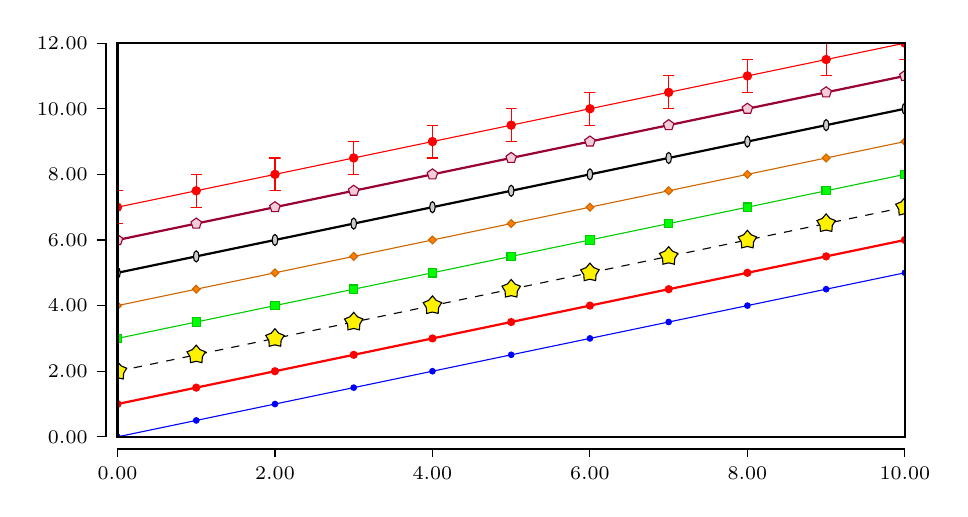
\begin{tikzpicture}[]
\begin{scope}[shift={(0.0,0.0)}]
\pgfsetxvec{\pgfpoint{1.0cm}{0cm}}
\pgfsetyvec{\pgfpoint{0cm}{0.41666666cm}}
\begin{scope}[shift={(0.0,0.0)}]
\begin{scope}[yshift=-0.15cm]
\draw[black] [shift={(0.0,0.0)}] (0,0) -- (0,-3pt) node[below]{ \scriptsize{\num[round-mode=places,round-precision=2]{0}}};
\draw[black] [shift={(2.0,0.0)}] (0,0) -- (0,-3pt) node[below]{ \scriptsize{\num[round-mode=places,round-precision=2]{2}}};
\draw[black] [shift={(4.0,0.0)}] (0,0) -- (0,-3pt) node[below]{ \scriptsize{\num[round-mode=places,round-precision=2]{4}}};
\draw[black] [shift={(6.0,0.0)}] (0,0) -- (0,-3pt) node[below]{ \scriptsize{\num[round-mode=places,round-precision=2]{6}}};
\draw[black] [shift={(8.0,0.0)}] (0,0) -- (0,-3pt) node[below]{ \scriptsize{\num[round-mode=places,round-precision=2]{8}}};
\draw[black] [shift={(10.0,0.0)}] (0,0) -- (0,-3pt) node[below]{ \scriptsize{\num[round-mode=places,round-precision=2]{10}}};
\end{scope}
\begin{scope}[xshift=-0.15cm]
\draw[black] [shift={(0.0,0.0)}] (0,0) -- (-3pt,0) node[left]{ \scriptsize{\num[round-mode=places,round-precision=2]{0}}};
\draw[black] [shift={(0.0,2.0)}] (0,0) -- (-3pt,0) node[left]{ \scriptsize{\num[round-mode=places,round-precision=2]{2}}};
\draw[black] [shift={(0.0,4.0)}] (0,0) -- (-3pt,0) node[left]{ \scriptsize{\num[round-mode=places,round-precision=2]{4}}};
\draw[black] [shift={(0.0,6.0)}] (0,0) -- (-3pt,0) node[left]{ \scriptsize{\num[round-mode=places,round-precision=2]{6}}};
\draw[black] [shift={(0.0,8.0)}] (0,0) -- (-3pt,0) node[left]{ \scriptsize{\num[round-mode=places,round-precision=2]{8}}};
\draw[black] [shift={(0.0,10.0)}] (0,0) -- (-3pt,0) node[left]{ \scriptsize{\num[round-mode=places,round-precision=2]{10}}};
\draw[black] [shift={(0.0,12.0)}] (0,0) -- (-3pt,0) node[left]{ \scriptsize{\num[round-mode=places,round-precision=2]{12}}};
\end{scope}
\end{scope}
\pgfsetxvec{\pgfpoint{1cm}{0cm}}
\pgfsetyvec{\pgfpoint{0cm}{1cm}}
\end{scope}
\begin{scope}[]
\clip (0.0,0.0) rectangle (10.0,5.0);
\begin{scope}[shift={(0.0,0.0)}]
\pgfsetxvec{\pgfpoint{1.0cm}{0cm}}
\pgfsetyvec{\pgfpoint{0cm}{0.41666666cm}}
\begin{scope}[shift={(0.0,0.0)}]
\begin{scope}[blue]
\pgfpathmoveto{ \pgfpointxy {0.0} {0.0}}
\pgfpathlineto{ \pgfpointxy {1.0} {0.5}}
\pgfpathlineto{ \pgfpointxy {2.0} {1.0}}
\pgfpathlineto{ \pgfpointxy {3.0} {1.5}}
\pgfpathlineto{ \pgfpointxy {4.0} {2.0}}
\pgfpathlineto{ \pgfpointxy {5.0} {2.5}}
\pgfpathlineto{ \pgfpointxy {6.0} {3.0}}
\pgfpathlineto{ \pgfpointxy {7.0} {3.5}}
\pgfpathlineto{ \pgfpointxy {8.0} {4.0}}
\pgfpathlineto{ \pgfpointxy {9.0} {4.5}}
\pgfpathlineto{ \pgfpointxy {10.0} {5.0}}
\pgfusepath{ stroke, }
\end{scope}
\node at (0.0,0.0) [circle,inner sep=0pt,minimum width =2pt,minimum height=2pt,fill=blue,draw=blue] {}; 
\node at (1.0,0.5) [circle,inner sep=0pt,minimum width =2pt,minimum height=2pt,fill=blue,draw=blue] {}; 
\node at (2.0,1.0) [circle,inner sep=0pt,minimum width =2pt,minimum height=2pt,fill=blue,draw=blue] {}; 
\node at (3.0,1.5) [circle,inner sep=0pt,minimum width =2pt,minimum height=2pt,fill=blue,draw=blue] {}; 
\node at (4.0,2.0) [circle,inner sep=0pt,minimum width =2pt,minimum height=2pt,fill=blue,draw=blue] {}; 
\node at (5.0,2.5) [circle,inner sep=0pt,minimum width =2pt,minimum height=2pt,fill=blue,draw=blue] {}; 
\node at (6.0,3.0) [circle,inner sep=0pt,minimum width =2pt,minimum height=2pt,fill=blue,draw=blue] {}; 
\node at (7.0,3.5) [circle,inner sep=0pt,minimum width =2pt,minimum height=2pt,fill=blue,draw=blue] {}; 
\node at (8.0,4.0) [circle,inner sep=0pt,minimum width =2pt,minimum height=2pt,fill=blue,draw=blue] {}; 
\node at (9.0,4.5) [circle,inner sep=0pt,minimum width =2pt,minimum height=2pt,fill=blue,draw=blue] {}; 
\node at (10.0,5.0) [circle,inner sep=0pt,minimum width =2pt,minimum height=2pt,fill=blue,draw=blue] {}; 
\begin{scope}[red,thick]
\pgfpathmoveto{ \pgfpointxy {0.0} {1.0}}
\pgfpathlineto{ \pgfpointxy {1.0} {1.5}}
\pgfpathlineto{ \pgfpointxy {2.0} {2.0}}
\pgfpathlineto{ \pgfpointxy {3.0} {2.5}}
\pgfpathlineto{ \pgfpointxy {4.0} {3.0}}
\pgfpathlineto{ \pgfpointxy {5.0} {3.5}}
\pgfpathlineto{ \pgfpointxy {6.0} {4.0}}
\pgfpathlineto{ \pgfpointxy {7.0} {4.5}}
\pgfpathlineto{ \pgfpointxy {8.0} {5.0}}
\pgfpathlineto{ \pgfpointxy {9.0} {5.5}}
\pgfpathlineto{ \pgfpointxy {10.0} {6.0}}
\pgfusepath{ stroke, }
\end{scope}
\node at (0.0,1.0) [circle,inner sep=0pt,minimum width =3pt,minimum height=3pt,fill=red] {}; 
\node at (1.0,1.5) [circle,inner sep=0pt,minimum width =3pt,minimum height=3pt,fill=red] {}; 
\node at (2.0,2.0) [circle,inner sep=0pt,minimum width =3pt,minimum height=3pt,fill=red] {}; 
\node at (3.0,2.5) [circle,inner sep=0pt,minimum width =3pt,minimum height=3pt,fill=red] {}; 
\node at (4.0,3.0) [circle,inner sep=0pt,minimum width =3pt,minimum height=3pt,fill=red] {}; 
\node at (5.0,3.5) [circle,inner sep=0pt,minimum width =3pt,minimum height=3pt,fill=red] {}; 
\node at (6.0,4.0) [circle,inner sep=0pt,minimum width =3pt,minimum height=3pt,fill=red] {}; 
\node at (7.0,4.5) [circle,inner sep=0pt,minimum width =3pt,minimum height=3pt,fill=red] {}; 
\node at (8.0,5.0) [circle,inner sep=0pt,minimum width =3pt,minimum height=3pt,fill=red] {}; 
\node at (9.0,5.5) [circle,inner sep=0pt,minimum width =3pt,minimum height=3pt,fill=red] {}; 
\node at (10.0,6.0) [circle,inner sep=0pt,minimum width =3pt,minimum height=3pt,fill=red] {}; 
\begin{scope}[black,dashed]
\pgfpathmoveto{ \pgfpointxy {0.0} {2.0}}
\pgfpathlineto{ \pgfpointxy {1.0} {2.5}}
\pgfpathlineto{ \pgfpointxy {2.0} {3.0}}
\pgfpathlineto{ \pgfpointxy {3.0} {3.5}}
\pgfpathlineto{ \pgfpointxy {4.0} {4.0}}
\pgfpathlineto{ \pgfpointxy {5.0} {4.5}}
\pgfpathlineto{ \pgfpointxy {6.0} {5.0}}
\pgfpathlineto{ \pgfpointxy {7.0} {5.5}}
\pgfpathlineto{ \pgfpointxy {8.0} {6.0}}
\pgfpathlineto{ \pgfpointxy {9.0} {6.5}}
\pgfpathlineto{ \pgfpointxy {10.0} {7.0}}
\pgfusepath{ stroke, }
\end{scope}
\node at (0.0,2.0) [star,star points=5,inner sep=0pt,minimum width =7pt,minimum height=7pt,draw=black,fill=yellow] {}; 
\node at (1.0,2.5) [star,star points=5,inner sep=0pt,minimum width =7pt,minimum height=7pt,draw=black,fill=yellow] {}; 
\node at (2.0,3.0) [star,star points=5,inner sep=0pt,minimum width =7pt,minimum height=7pt,draw=black,fill=yellow] {}; 
\node at (3.0,3.5) [star,star points=5,inner sep=0pt,minimum width =7pt,minimum height=7pt,draw=black,fill=yellow] {}; 
\node at (4.0,4.0) [star,star points=5,inner sep=0pt,minimum width =7pt,minimum height=7pt,draw=black,fill=yellow] {}; 
\node at (5.0,4.5) [star,star points=5,inner sep=0pt,minimum width =7pt,minimum height=7pt,draw=black,fill=yellow] {}; 
\node at (6.0,5.0) [star,star points=5,inner sep=0pt,minimum width =7pt,minimum height=7pt,draw=black,fill=yellow] {}; 
\node at (7.0,5.5) [star,star points=5,inner sep=0pt,minimum width =7pt,minimum height=7pt,draw=black,fill=yellow] {}; 
\node at (8.0,6.0) [star,star points=5,inner sep=0pt,minimum width =7pt,minimum height=7pt,draw=black,fill=yellow] {}; 
\node at (9.0,6.5) [star,star points=5,inner sep=0pt,minimum width =7pt,minimum height=7pt,draw=black,fill=yellow] {}; 
\node at (10.0,7.0) [star,star points=5,inner sep=0pt,minimum width =7pt,minimum height=7pt,draw=black,fill=yellow] {}; 
\begin{scope}[green!80!black]
\pgfpathmoveto{ \pgfpointxy {0.0} {3.0}}
\pgfpathlineto{ \pgfpointxy {1.0} {3.5}}
\pgfpathlineto{ \pgfpointxy {2.0} {4.0}}
\pgfpathlineto{ \pgfpointxy {3.0} {4.5}}
\pgfpathlineto{ \pgfpointxy {4.0} {5.0}}
\pgfpathlineto{ \pgfpointxy {5.0} {5.5}}
\pgfpathlineto{ \pgfpointxy {6.0} {6.0}}
\pgfpathlineto{ \pgfpointxy {7.0} {6.5}}
\pgfpathlineto{ \pgfpointxy {8.0} {7.0}}
\pgfpathlineto{ \pgfpointxy {9.0} {7.5}}
\pgfpathlineto{ \pgfpointxy {10.0} {8.0}}
\pgfusepath{ stroke, }
\end{scope}
\node at (0.0,3.0) [rectangle,inner sep=0pt,minimum width =3pt,minimum height=3pt,draw=green!80!black,fill=green] {}; 
\node at (1.0,3.5) [rectangle,inner sep=0pt,minimum width =3pt,minimum height=3pt,draw=green!80!black,fill=green] {}; 
\node at (2.0,4.0) [rectangle,inner sep=0pt,minimum width =3pt,minimum height=3pt,draw=green!80!black,fill=green] {}; 
\node at (3.0,4.5) [rectangle,inner sep=0pt,minimum width =3pt,minimum height=3pt,draw=green!80!black,fill=green] {}; 
\node at (4.0,5.0) [rectangle,inner sep=0pt,minimum width =3pt,minimum height=3pt,draw=green!80!black,fill=green] {}; 
\node at (5.0,5.5) [rectangle,inner sep=0pt,minimum width =3pt,minimum height=3pt,draw=green!80!black,fill=green] {}; 
\node at (6.0,6.0) [rectangle,inner sep=0pt,minimum width =3pt,minimum height=3pt,draw=green!80!black,fill=green] {}; 
\node at (7.0,6.5) [rectangle,inner sep=0pt,minimum width =3pt,minimum height=3pt,draw=green!80!black,fill=green] {}; 
\node at (8.0,7.0) [rectangle,inner sep=0pt,minimum width =3pt,minimum height=3pt,draw=green!80!black,fill=green] {}; 
\node at (9.0,7.5) [rectangle,inner sep=0pt,minimum width =3pt,minimum height=3pt,draw=green!80!black,fill=green] {}; 
\node at (10.0,8.0) [rectangle,inner sep=0pt,minimum width =3pt,minimum height=3pt,draw=green!80!black,fill=green] {}; 
\begin{scope}[orange!80!black]
\pgfpathmoveto{ \pgfpointxy {0.0} {4.0}}
\pgfpathlineto{ \pgfpointxy {1.0} {4.5}}
\pgfpathlineto{ \pgfpointxy {2.0} {5.0}}
\pgfpathlineto{ \pgfpointxy {3.0} {5.5}}
\pgfpathlineto{ \pgfpointxy {4.0} {6.0}}
\pgfpathlineto{ \pgfpointxy {5.0} {6.5}}
\pgfpathlineto{ \pgfpointxy {6.0} {7.0}}
\pgfpathlineto{ \pgfpointxy {7.0} {7.5}}
\pgfpathlineto{ \pgfpointxy {8.0} {8.0}}
\pgfpathlineto{ \pgfpointxy {9.0} {8.5}}
\pgfpathlineto{ \pgfpointxy {10.0} {9.0}}
\pgfusepath{ stroke, }
\end{scope}
\node at (0.0,4.0) [diamond,inner sep=0pt,minimum width =3pt,minimum height=3pt,draw=orange!80!black,fill=orange] {}; 
\node at (1.0,4.5) [diamond,inner sep=0pt,minimum width =3pt,minimum height=3pt,draw=orange!80!black,fill=orange] {}; 
\node at (2.0,5.0) [diamond,inner sep=0pt,minimum width =3pt,minimum height=3pt,draw=orange!80!black,fill=orange] {}; 
\node at (3.0,5.5) [diamond,inner sep=0pt,minimum width =3pt,minimum height=3pt,draw=orange!80!black,fill=orange] {}; 
\node at (4.0,6.0) [diamond,inner sep=0pt,minimum width =3pt,minimum height=3pt,draw=orange!80!black,fill=orange] {}; 
\node at (5.0,6.5) [diamond,inner sep=0pt,minimum width =3pt,minimum height=3pt,draw=orange!80!black,fill=orange] {}; 
\node at (6.0,7.0) [diamond,inner sep=0pt,minimum width =3pt,minimum height=3pt,draw=orange!80!black,fill=orange] {}; 
\node at (7.0,7.5) [diamond,inner sep=0pt,minimum width =3pt,minimum height=3pt,draw=orange!80!black,fill=orange] {}; 
\node at (8.0,8.0) [diamond,inner sep=0pt,minimum width =3pt,minimum height=3pt,draw=orange!80!black,fill=orange] {}; 
\node at (9.0,8.5) [diamond,inner sep=0pt,minimum width =3pt,minimum height=3pt,draw=orange!80!black,fill=orange] {}; 
\node at (10.0,9.0) [diamond,inner sep=0pt,minimum width =3pt,minimum height=3pt,draw=orange!80!black,fill=orange] {}; 
\begin{scope}[black,thick]
\pgfpathmoveto{ \pgfpointxy {0.0} {5.0}}
\pgfpathlineto{ \pgfpointxy {1.0} {5.5}}
\pgfpathlineto{ \pgfpointxy {2.0} {6.0}}
\pgfpathlineto{ \pgfpointxy {3.0} {6.5}}
\pgfpathlineto{ \pgfpointxy {4.0} {7.0}}
\pgfpathlineto{ \pgfpointxy {5.0} {7.5}}
\pgfpathlineto{ \pgfpointxy {6.0} {8.0}}
\pgfpathlineto{ \pgfpointxy {7.0} {8.5}}
\pgfpathlineto{ \pgfpointxy {8.0} {9.0}}
\pgfpathlineto{ \pgfpointxy {9.0} {9.5}}
\pgfpathlineto{ \pgfpointxy {10.0} {10.0}}
\pgfusepath{ stroke, }
\end{scope}
\node at (0.0,5.0) [ellipse,inner sep=0pt,minimum width =2pt,minimum height=4pt,draw=black,fill=black!20] {}; 
\node at (1.0,5.5) [ellipse,inner sep=0pt,minimum width =2pt,minimum height=4pt,draw=black,fill=black!20] {}; 
\node at (2.0,6.0) [ellipse,inner sep=0pt,minimum width =2pt,minimum height=4pt,draw=black,fill=black!20] {}; 
\node at (3.0,6.5) [ellipse,inner sep=0pt,minimum width =2pt,minimum height=4pt,draw=black,fill=black!20] {}; 
\node at (4.0,7.0) [ellipse,inner sep=0pt,minimum width =2pt,minimum height=4pt,draw=black,fill=black!20] {}; 
\node at (5.0,7.5) [ellipse,inner sep=0pt,minimum width =2pt,minimum height=4pt,draw=black,fill=black!20] {}; 
\node at (6.0,8.0) [ellipse,inner sep=0pt,minimum width =2pt,minimum height=4pt,draw=black,fill=black!20] {}; 
\node at (7.0,8.5) [ellipse,inner sep=0pt,minimum width =2pt,minimum height=4pt,draw=black,fill=black!20] {}; 
\node at (8.0,9.0) [ellipse,inner sep=0pt,minimum width =2pt,minimum height=4pt,draw=black,fill=black!20] {}; 
\node at (9.0,9.5) [ellipse,inner sep=0pt,minimum width =2pt,minimum height=4pt,draw=black,fill=black!20] {}; 
\node at (10.0,10.0) [ellipse,inner sep=0pt,minimum width =2pt,minimum height=4pt,draw=black,fill=black!20] {}; 
\begin{scope}[purple!80!black,thick]
\pgfpathmoveto{ \pgfpointxy {0.0} {6.0}}
\pgfpathlineto{ \pgfpointxy {1.0} {6.5}}
\pgfpathlineto{ \pgfpointxy {2.0} {7.0}}
\pgfpathlineto{ \pgfpointxy {3.0} {7.5}}
\pgfpathlineto{ \pgfpointxy {4.0} {8.0}}
\pgfpathlineto{ \pgfpointxy {5.0} {8.5}}
\pgfpathlineto{ \pgfpointxy {6.0} {9.0}}
\pgfpathlineto{ \pgfpointxy {7.0} {9.5}}
\pgfpathlineto{ \pgfpointxy {8.0} {10.0}}
\pgfpathlineto{ \pgfpointxy {9.0} {10.5}}
\pgfpathlineto{ \pgfpointxy {10.0} {11.0}}
\pgfusepath{ stroke, }
\end{scope}
\node at (0.0,6.0) [regular polygon,regular polygon sides=5,inner sep=0pt,minimum width =4pt,minimum height=4pt,draw=purple!80!black,fill=purple!20] {}; 
\node at (1.0,6.5) [regular polygon,regular polygon sides=5,inner sep=0pt,minimum width =4pt,minimum height=4pt,draw=purple!80!black,fill=purple!20] {}; 
\node at (2.0,7.0) [regular polygon,regular polygon sides=5,inner sep=0pt,minimum width =4pt,minimum height=4pt,draw=purple!80!black,fill=purple!20] {}; 
\node at (3.0,7.5) [regular polygon,regular polygon sides=5,inner sep=0pt,minimum width =4pt,minimum height=4pt,draw=purple!80!black,fill=purple!20] {}; 
\node at (4.0,8.0) [regular polygon,regular polygon sides=5,inner sep=0pt,minimum width =4pt,minimum height=4pt,draw=purple!80!black,fill=purple!20] {}; 
\node at (5.0,8.5) [regular polygon,regular polygon sides=5,inner sep=0pt,minimum width =4pt,minimum height=4pt,draw=purple!80!black,fill=purple!20] {}; 
\node at (6.0,9.0) [regular polygon,regular polygon sides=5,inner sep=0pt,minimum width =4pt,minimum height=4pt,draw=purple!80!black,fill=purple!20] {}; 
\node at (7.0,9.5) [regular polygon,regular polygon sides=5,inner sep=0pt,minimum width =4pt,minimum height=4pt,draw=purple!80!black,fill=purple!20] {}; 
\node at (8.0,10.0) [regular polygon,regular polygon sides=5,inner sep=0pt,minimum width =4pt,minimum height=4pt,draw=purple!80!black,fill=purple!20] {}; 
\node at (9.0,10.5) [regular polygon,regular polygon sides=5,inner sep=0pt,minimum width =4pt,minimum height=4pt,draw=purple!80!black,fill=purple!20] {}; 
\node at (10.0,11.0) [regular polygon,regular polygon sides=5,inner sep=0pt,minimum width =4pt,minimum height=4pt,draw=purple!80!black,fill=purple!20] {}; 
\begin{scope}[red]
\pgfpathmoveto{ \pgfpointxy {0.0} {7.0}}
\pgfpathlineto{ \pgfpointxy {1.0} {7.5}}
\pgfpathlineto{ \pgfpointxy {2.0} {8.0}}
\pgfpathlineto{ \pgfpointxy {3.0} {8.5}}
\pgfpathlineto{ \pgfpointxy {4.0} {9.0}}
\pgfpathlineto{ \pgfpointxy {5.0} {9.5}}
\pgfpathlineto{ \pgfpointxy {6.0} {10.0}}
\pgfpathlineto{ \pgfpointxy {7.0} {10.5}}
\pgfpathlineto{ \pgfpointxy {8.0} {11.0}}
\pgfpathlineto{ \pgfpointxy {9.0} {11.5}}
\pgfpathlineto{ \pgfpointxy {10.0} {12.0}}
\pgfusepath{ stroke, }
\end{scope}
\begin{scope}[draw=red,fill=red]
\pgfpointadd{\pgfpointxy {0.0} {7.5}} {\pgfpoint{-2pt}{0}}\pgfpathmoveto{ NIL }
\pgfpointadd{\pgfpointxy {0.0} {7.5}} {\pgfpoint{2pt}{0}}\pgfpathlineto{ NIL }
\pgfpointadd{\pgfpointxy {0.0} {7.5}} {\pgfpoint{0pt}{0}}\pgfpathlineto{ NIL }
\pgfpointadd{\pgfpointxy {0.0} {6.5}} {\pgfpoint{0pt}{0}}\pgfpathlineto{ NIL }
\pgfpointadd{\pgfpointxy {0.0} {6.5}} {\pgfpoint{-2pt}{0}}\pgfpathlineto{ NIL }
\pgfpointadd{\pgfpointxy {0.0} {6.5}} {\pgfpoint{2pt}{0}}\pgfpathlineto{ NIL }
\pgfusepath{ stroke, }
\node at (0.0,7.0) [circle,inner sep=0pt,minimum width =3pt,minimum height=3pt,draw=red,fill=red] {}; 
\end{scope}
\begin{scope}[draw=red,fill=red]
\pgfpointadd{\pgfpointxy {1.0} {8.0}} {\pgfpoint{-2pt}{0}}\pgfpathmoveto{ NIL }
\pgfpointadd{\pgfpointxy {1.0} {8.0}} {\pgfpoint{2pt}{0}}\pgfpathlineto{ NIL }
\pgfpointadd{\pgfpointxy {1.0} {8.0}} {\pgfpoint{0pt}{0}}\pgfpathlineto{ NIL }
\pgfpointadd{\pgfpointxy {1.0} {7.0}} {\pgfpoint{0pt}{0}}\pgfpathlineto{ NIL }
\pgfpointadd{\pgfpointxy {1.0} {7.0}} {\pgfpoint{-2pt}{0}}\pgfpathlineto{ NIL }
\pgfpointadd{\pgfpointxy {1.0} {7.0}} {\pgfpoint{2pt}{0}}\pgfpathlineto{ NIL }
\pgfusepath{ stroke, }
\node at (1.0,7.5) [circle,inner sep=0pt,minimum width =3pt,minimum height=3pt,draw=red,fill=red] {}; 
\end{scope}
\begin{scope}[draw=red,fill=red]
\pgfpointadd{\pgfpointxy {2.0} {8.5}} {\pgfpoint{-2pt}{0}}\pgfpathmoveto{ NIL }
\pgfpointadd{\pgfpointxy {2.0} {8.5}} {\pgfpoint{2pt}{0}}\pgfpathlineto{ NIL }
\pgfpointadd{\pgfpointxy {2.0} {8.5}} {\pgfpoint{0pt}{0}}\pgfpathlineto{ NIL }
\pgfpointadd{\pgfpointxy {2.0} {7.5}} {\pgfpoint{0pt}{0}}\pgfpathlineto{ NIL }
\pgfpointadd{\pgfpointxy {2.0} {7.5}} {\pgfpoint{-2pt}{0}}\pgfpathlineto{ NIL }
\pgfpointadd{\pgfpointxy {2.0} {7.5}} {\pgfpoint{2pt}{0}}\pgfpathlineto{ NIL }
\pgfusepath{ stroke, }
\node at (2.0,8.0) [circle,inner sep=0pt,minimum width =3pt,minimum height=3pt,draw=red,fill=red] {}; 
\end{scope}
\begin{scope}[draw=red,fill=red]
\pgfpointadd{\pgfpointxy {3.0} {9.0}} {\pgfpoint{-2pt}{0}}\pgfpathmoveto{ NIL }
\pgfpointadd{\pgfpointxy {3.0} {9.0}} {\pgfpoint{2pt}{0}}\pgfpathlineto{ NIL }
\pgfpointadd{\pgfpointxy {3.0} {9.0}} {\pgfpoint{0pt}{0}}\pgfpathlineto{ NIL }
\pgfpointadd{\pgfpointxy {3.0} {8.0}} {\pgfpoint{0pt}{0}}\pgfpathlineto{ NIL }
\pgfpointadd{\pgfpointxy {3.0} {8.0}} {\pgfpoint{-2pt}{0}}\pgfpathlineto{ NIL }
\pgfpointadd{\pgfpointxy {3.0} {8.0}} {\pgfpoint{2pt}{0}}\pgfpathlineto{ NIL }
\pgfusepath{ stroke, }
\node at (3.0,8.5) [circle,inner sep=0pt,minimum width =3pt,minimum height=3pt,draw=red,fill=red] {}; 
\end{scope}
\begin{scope}[draw=red,fill=red]
\pgfpointadd{\pgfpointxy {4.0} {9.5}} {\pgfpoint{-2pt}{0}}\pgfpathmoveto{ NIL }
\pgfpointadd{\pgfpointxy {4.0} {9.5}} {\pgfpoint{2pt}{0}}\pgfpathlineto{ NIL }
\pgfpointadd{\pgfpointxy {4.0} {9.5}} {\pgfpoint{0pt}{0}}\pgfpathlineto{ NIL }
\pgfpointadd{\pgfpointxy {4.0} {8.5}} {\pgfpoint{0pt}{0}}\pgfpathlineto{ NIL }
\pgfpointadd{\pgfpointxy {4.0} {8.5}} {\pgfpoint{-2pt}{0}}\pgfpathlineto{ NIL }
\pgfpointadd{\pgfpointxy {4.0} {8.5}} {\pgfpoint{2pt}{0}}\pgfpathlineto{ NIL }
\pgfusepath{ stroke, }
\node at (4.0,9.0) [circle,inner sep=0pt,minimum width =3pt,minimum height=3pt,draw=red,fill=red] {}; 
\end{scope}
\begin{scope}[draw=red,fill=red]
\pgfpointadd{\pgfpointxy {5.0} {10.0}} {\pgfpoint{-2pt}{0}}\pgfpathmoveto{ NIL }
\pgfpointadd{\pgfpointxy {5.0} {10.0}} {\pgfpoint{2pt}{0}}\pgfpathlineto{ NIL }
\pgfpointadd{\pgfpointxy {5.0} {10.0}} {\pgfpoint{0pt}{0}}\pgfpathlineto{ NIL }
\pgfpointadd{\pgfpointxy {5.0} {9.0}} {\pgfpoint{0pt}{0}}\pgfpathlineto{ NIL }
\pgfpointadd{\pgfpointxy {5.0} {9.0}} {\pgfpoint{-2pt}{0}}\pgfpathlineto{ NIL }
\pgfpointadd{\pgfpointxy {5.0} {9.0}} {\pgfpoint{2pt}{0}}\pgfpathlineto{ NIL }
\pgfusepath{ stroke, }
\node at (5.0,9.5) [circle,inner sep=0pt,minimum width =3pt,minimum height=3pt,draw=red,fill=red] {}; 
\end{scope}
\begin{scope}[draw=red,fill=red]
\pgfpointadd{\pgfpointxy {6.0} {10.5}} {\pgfpoint{-2pt}{0}}\pgfpathmoveto{ NIL }
\pgfpointadd{\pgfpointxy {6.0} {10.5}} {\pgfpoint{2pt}{0}}\pgfpathlineto{ NIL }
\pgfpointadd{\pgfpointxy {6.0} {10.5}} {\pgfpoint{0pt}{0}}\pgfpathlineto{ NIL }
\pgfpointadd{\pgfpointxy {6.0} {9.5}} {\pgfpoint{0pt}{0}}\pgfpathlineto{ NIL }
\pgfpointadd{\pgfpointxy {6.0} {9.5}} {\pgfpoint{-2pt}{0}}\pgfpathlineto{ NIL }
\pgfpointadd{\pgfpointxy {6.0} {9.5}} {\pgfpoint{2pt}{0}}\pgfpathlineto{ NIL }
\pgfusepath{ stroke, }
\node at (6.0,10.0) [circle,inner sep=0pt,minimum width =3pt,minimum height=3pt,draw=red,fill=red] {}; 
\end{scope}
\begin{scope}[draw=red,fill=red]
\pgfpointadd{\pgfpointxy {7.0} {11.0}} {\pgfpoint{-2pt}{0}}\pgfpathmoveto{ NIL }
\pgfpointadd{\pgfpointxy {7.0} {11.0}} {\pgfpoint{2pt}{0}}\pgfpathlineto{ NIL }
\pgfpointadd{\pgfpointxy {7.0} {11.0}} {\pgfpoint{0pt}{0}}\pgfpathlineto{ NIL }
\pgfpointadd{\pgfpointxy {7.0} {10.0}} {\pgfpoint{0pt}{0}}\pgfpathlineto{ NIL }
\pgfpointadd{\pgfpointxy {7.0} {10.0}} {\pgfpoint{-2pt}{0}}\pgfpathlineto{ NIL }
\pgfpointadd{\pgfpointxy {7.0} {10.0}} {\pgfpoint{2pt}{0}}\pgfpathlineto{ NIL }
\pgfusepath{ stroke, }
\node at (7.0,10.5) [circle,inner sep=0pt,minimum width =3pt,minimum height=3pt,draw=red,fill=red] {}; 
\end{scope}
\begin{scope}[draw=red,fill=red]
\pgfpointadd{\pgfpointxy {8.0} {11.5}} {\pgfpoint{-2pt}{0}}\pgfpathmoveto{ NIL }
\pgfpointadd{\pgfpointxy {8.0} {11.5}} {\pgfpoint{2pt}{0}}\pgfpathlineto{ NIL }
\pgfpointadd{\pgfpointxy {8.0} {11.5}} {\pgfpoint{0pt}{0}}\pgfpathlineto{ NIL }
\pgfpointadd{\pgfpointxy {8.0} {10.5}} {\pgfpoint{0pt}{0}}\pgfpathlineto{ NIL }
\pgfpointadd{\pgfpointxy {8.0} {10.5}} {\pgfpoint{-2pt}{0}}\pgfpathlineto{ NIL }
\pgfpointadd{\pgfpointxy {8.0} {10.5}} {\pgfpoint{2pt}{0}}\pgfpathlineto{ NIL }
\pgfusepath{ stroke, }
\node at (8.0,11.0) [circle,inner sep=0pt,minimum width =3pt,minimum height=3pt,draw=red,fill=red] {}; 
\end{scope}
\begin{scope}[draw=red,fill=red]
\pgfpointadd{\pgfpointxy {9.0} {12.0}} {\pgfpoint{-2pt}{0}}\pgfpathmoveto{ NIL }
\pgfpointadd{\pgfpointxy {9.0} {12.0}} {\pgfpoint{2pt}{0}}\pgfpathlineto{ NIL }
\pgfpointadd{\pgfpointxy {9.0} {12.0}} {\pgfpoint{0pt}{0}}\pgfpathlineto{ NIL }
\pgfpointadd{\pgfpointxy {9.0} {11.0}} {\pgfpoint{0pt}{0}}\pgfpathlineto{ NIL }
\pgfpointadd{\pgfpointxy {9.0} {11.0}} {\pgfpoint{-2pt}{0}}\pgfpathlineto{ NIL }
\pgfpointadd{\pgfpointxy {9.0} {11.0}} {\pgfpoint{2pt}{0}}\pgfpathlineto{ NIL }
\pgfusepath{ stroke, }
\node at (9.0,11.5) [circle,inner sep=0pt,minimum width =3pt,minimum height=3pt,draw=red,fill=red] {}; 
\end{scope}
\begin{scope}[draw=red,fill=red]
\pgfpointadd{\pgfpointxy {10.0} {12.5}} {\pgfpoint{-2pt}{0}}\pgfpathmoveto{ NIL }
\pgfpointadd{\pgfpointxy {10.0} {12.5}} {\pgfpoint{2pt}{0}}\pgfpathlineto{ NIL }
\pgfpointadd{\pgfpointxy {10.0} {12.5}} {\pgfpoint{0pt}{0}}\pgfpathlineto{ NIL }
\pgfpointadd{\pgfpointxy {10.0} {11.5}} {\pgfpoint{0pt}{0}}\pgfpathlineto{ NIL }
\pgfpointadd{\pgfpointxy {10.0} {11.5}} {\pgfpoint{-2pt}{0}}\pgfpathlineto{ NIL }
\pgfpointadd{\pgfpointxy {10.0} {11.5}} {\pgfpoint{2pt}{0}}\pgfpathlineto{ NIL }
\pgfusepath{ stroke, }
\node at (10.0,12.0) [circle,inner sep=0pt,minimum width =3pt,minimum height=3pt,draw=red,fill=red] {}; 
\end{scope}
\end{scope}
\pgfsetxvec{\pgfpoint{1cm}{0cm}}
\pgfsetyvec{\pgfpoint{0cm}{1cm}}
\end{scope}
\end{scope}
\draw[black,thick] (0.0,-0.15) -- (10.0,-0.15);
\draw[black,thick] (-0.15,0.0) -- (-0.15,5.0);
\begin{scope}[thick,black,fill=white]
\pgfpathmoveto{ \pgfpointxy {0.0} {0.0}}
\pgfpathlineto{ \pgfpointxy {10.0} {0.0}}
\pgfpathlineto{ \pgfpointxy {10.0} {5.0}}
\pgfpathlineto{ \pgfpointxy {0.0} {5.0}}
\pgfpathclose
\pgfusepath{ stroke, }
\end{scope}
\end{tikzpicture}
%%% Local Variables: 
%%% mode: latex 
%%% TeX-master: "master" 
%%% End:


\captionsetup{singlelinecheck=off}
\caption[asdf]{Different styles of lines and nodes. The styles are just regular tikz options.}
\end{figure}
\begin{figure}[H]
\centering
\documentclass{standalone}
\ifx\HCode\UnDef\else\def\pgfsysdriver{pgfsys-tex4ht.def}\fi
\usepackage[usenames,dvipsnames,svgnames,table]{xcolor}
\usepackage{tikz}
\usepackage{color}
\usepackage{siunitx}
\usetikzlibrary{arrows,shapes}
\begin{document}
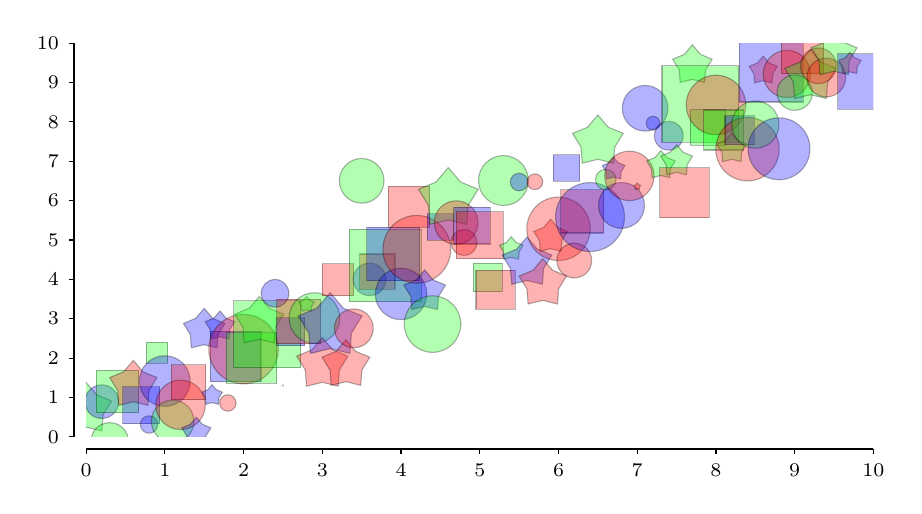
\begin{tikzpicture}
\begin{scope}[]
\pgfpointadd{\pgfpointxy {0.0} {0.0}} {\pgfpoint{0cm}{0cm}}\pgfpathmoveto{ NIL }
\pgfpointadd{\pgfpointxy {0.0} {0.0}} {\pgfpoint{10cm}{0cm}}\pgfpathlineto{ NIL }
\pgfpointadd{\pgfpointxy {0.0} {0.0}} {\pgfpoint{10cm}{5cm}}\pgfpathlineto{ NIL }
\pgfpointadd{\pgfpointxy {0.0} {0.0}} {\pgfpoint{0cm}{5cm}}\pgfpathlineto{ NIL }
\pgfpathclose
\pgfusepath{  clip, }
\begin{scope}[shift={(0.0,0.0)}]
\pgfsetxvec{\pgfpoint{1.0cm}{0cm}}
\pgfsetyvec{\pgfpoint{0cm}{0.5cm}}
\begin{scope}[shift={(0.0,0.0)}]
\node at (0.0,0.7006110756122909) [draw=black,fill=green,opacity=0.3,star,inner sep=0.0mm,minimum width =6.800587496850904mm,minimum height=6.800587496850904mm] {};
\node at (0.1,-0.7734106387051958) [draw=black,fill=green,opacity=0.3,star,inner sep=0.0mm,minimum width =3.6460143198852952mm,minimum height=3.6460143198852952mm] {};
\node at (0.2,0.8936623412927944) [draw=black,fill=blue,opacity=0.3,circle,inner sep=0.0mm,minimum width =4.272260443846609mm,minimum height=4.272260443846609mm] {};
\node at (0.3,-0.11494552503266542) [draw=black,fill=green,opacity=0.3,circle,inner sep=0.0mm,minimum width =4.752905216170019mm,minimum height=4.752905216170019mm] {};
\node at (0.4,1.150349541366745) [draw=black,fill=green,opacity=0.3,rectangle,inner sep=0.0mm,minimum width =5.378692570370324mm,minimum height=5.378692570370324mm] {};
\node at (0.5,-1.8588294510295857) [draw=black,fill=red,opacity=0.3,circle,inner sep=0.0mm,minimum width =5.952965504524424mm,minimum height=5.952965504524424mm] {};
\node at (0.6,1.3106837531472841) [draw=black,fill=red,opacity=0.3,star,inner sep=0.0mm,minimum width =6.315038332090647mm,minimum height=6.315038332090647mm] {};
\node at (0.7,0.8044580736841929) [draw=black,fill=blue,opacity=0.3,rectangle,inner sep=0.0mm,minimum width =4.731654041668135mm,minimum height=4.731654041668135mm] {};
\node at (0.8,0.31356219753880626) [draw=black,fill=blue,opacity=0.3,circle,inner sep=0.0mm,minimum width =2.220868006425221mm,minimum height=2.220868006425221mm] {};
\node at (0.90000004,2.1329623554392843) [draw=black,fill=green,opacity=0.3,rectangle,inner sep=0.0mm,minimum width =2.6819606796927187mm,minimum height=2.6819606796927187mm] {};
\node at (1.0,1.4159074987429303) [draw=black,fill=blue,opacity=0.3,circle,inner sep=0.0mm,minimum width =6.442954524709304mm,minimum height=6.442954524709304mm] {};
\node at (1.1,0.39295316234538624) [draw=black,fill=green,opacity=0.3,circle,inner sep=0.0mm,minimum width =5.399756727494323mm,minimum height=5.399756727494323mm] {};
\node at (1.2,0.8132344213873199) [draw=black,fill=red,opacity=0.3,circle,inner sep=0.0mm,minimum width =6.287295603642487mm,minimum height=6.287295603642487mm] {};
\node at (1.3000001,1.3872414968679347) [draw=black,fill=red,opacity=0.3,rectangle,inner sep=0.0mm,minimum width =4.409969468970658mm,minimum height=4.409969468970658mm] {};
\node at (1.4,0.1090123422278444) [draw=black,fill=blue,opacity=0.3,star,inner sep=0.0mm,minimum width =3.890683836470598mm,minimum height=3.890683836470598mm] {};
\node at (1.5,2.709103305949749) [draw=black,fill=blue,opacity=0.3,star,inner sep=0.0mm,minimum width =5.542198749418023mm,minimum height=5.542198749418023mm] {};
\node at (1.6,1.0500102467760244) [draw=black,fill=blue,opacity=0.3,star,inner sep=0.0mm,minimum width =2.741419975172315mm,minimum height=2.741419975172315mm] {};
\node at (1.7,2.804268401979424) [draw=black,fill=blue,opacity=0.3,star,inner sep=0.0mm,minimum width =3.9322501146273385mm,minimum height=3.9322501146273385mm] {};
\node at (1.8000001,0.8604649480672137) [draw=black,fill=red,opacity=0.3,circle,inner sep=0.0mm,minimum width =2.090570155891645mm,minimum height=2.090570155891645mm] {};
\node at (1.9,2.0407167342406702) [draw=black,fill=blue,opacity=0.3,rectangle,inner sep=0.0mm,minimum width =6.435583612838957mm,minimum height=6.435583612838957mm] {};
\node at (2.0,2.2286922355247976) [draw=black,fill=red,opacity=0.3,circle,inner sep=0.0mm,minimum width =8.832062398405533mm,minimum height=8.832062398405533mm] {};
\node at (2.1000001,2.000614315353244) [draw=black,fill=green,opacity=0.3,rectangle,inner sep=0.0mm,minimum width =6.388258996727354mm,minimum height=6.388258996727354mm] {};
\node at (2.2,2.9135575687932036) [draw=black,fill=green,opacity=0.3,star,inner sep=0.0mm,minimum width =6.503302028106489mm,minimum height=6.503302028106489mm] {};
\node at (2.3,2.6057336498405617) [draw=black,fill=green,opacity=0.3,rectangle,inner sep=0.0mm,minimum width =8.532957621356363mm,minimum height=8.532957621356363mm] {};
\node at (2.4,3.644968288436833) [draw=black,fill=blue,opacity=0.3,circle,inner sep=0.0mm,minimum width =3.5184462877320484mm,minimum height=3.5184462877320484mm] {};
\node at (2.5,1.3041485524642158) [draw=black,fill=red,opacity=0.3,star,inner sep=0.0mm,minimum width =0.1mm,minimum height=0.1mm] {};
\node at (2.6000001,2.667533754247742) [draw=black,fill=blue,opacity=0.3,rectangle,inner sep=0.0mm,minimum width =3.570086353410753mm,minimum height=3.570086353410753mm] {};
\node at (2.7,2.931016904802913) [draw=black,fill=red,opacity=0.3,rectangle,inner sep=0.0mm,minimum width =5.6091544426281805mm,minimum height=5.6091544426281805mm] {};
\node at (2.8,3.3603908893740035) [draw=black,fill=green,opacity=0.3,star,inner sep=0.0mm,minimum width =2.0136506057312813mm,minimum height=2.0136506057312813mm] {};
\node at (2.9,3.0166066169551957) [draw=black,fill=green,opacity=0.3,circle,inner sep=0.0mm,minimum width =6.4448519208068795mm,minimum height=6.4448519208068795mm] {};
\node at (3.0,1.8390865566362826) [draw=black,fill=red,opacity=0.3,star,inner sep=0.0mm,minimum width =6.829311725505772mm,minimum height=6.829311725505772mm] {};
\node at (3.1000001,2.8090410129452135) [draw=black,fill=blue,opacity=0.3,star,inner sep=0.0mm,minimum width =8.526654123325148mm,minimum height=8.526654123325148mm] {};
\node at (3.2,3.9904474878671072) [draw=black,fill=red,opacity=0.3,rectangle,inner sep=0.0mm,minimum width =4.028381917972839mm,minimum height=4.028381917972839mm] {};
\node at (3.3,1.826071884695202) [draw=black,fill=red,opacity=0.3,star,inner sep=0.0mm,minimum width =6.384264845787511mm,minimum height=6.384264845787511mm] {};
\node at (3.4,2.756052548182273) [draw=black,fill=red,opacity=0.3,circle,inner sep=0.0mm,minimum width =4.926370312479602mm,minimum height=4.926370312479602mm] {};
\node at (3.5,6.5025300185625525) [draw=black,fill=green,opacity=0.3,circle,inner sep=0.0mm,minimum width =5.666485070612519mm,minimum height=5.666485070612519mm] {};
\node at (3.6000001,4.001097507639919) [draw=black,fill=blue,opacity=0.3,circle,inner sep=0.0mm,minimum width =4.138853579394104mm,minimum height=4.138853579394104mm] {};
\node at (3.7,4.19701461175223) [draw=black,fill=red,opacity=0.3,rectangle,inner sep=0.0mm,minimum width =4.472865794162527mm,minimum height=4.472865794162527mm] {};
\node at (3.8,4.350897011030634) [draw=black,fill=green,opacity=0.3,rectangle,inner sep=0.0mm,minimum width =9.158076511100287mm,minimum height=9.158076511100287mm] {};
\node at (3.9,4.642078870376014) [draw=black,fill=blue,opacity=0.3,rectangle,inner sep=0.0mm,minimum width =6.753169795357893mm,minimum height=6.753169795357893mm] {};
\node at (4.0,3.6289117627006258) [draw=black,fill=blue,opacity=0.3,circle,inner sep=0.0mm,minimum width =6.534480556075062mm,minimum height=6.534480556075062mm] {};
\node at (4.1,5.845577054396422) [draw=black,fill=red,opacity=0.3,rectangle,inner sep=0.0mm,minimum width =5.228700941694266mm,minimum height=5.228700941694266mm] {};
\node at (4.2000003,4.761594535940161) [draw=black,fill=red,opacity=0.3,circle,inner sep=0.0mm,minimum width =8.616717667652617mm,minimum height=8.616717667652617mm] {};
\node at (4.3,3.6832125800853603) [draw=black,fill=blue,opacity=0.3,star,inner sep=0.0mm,minimum width =5.5685232481589555mm,minimum height=5.5685232481589555mm] {};
\node at (4.4,2.864283362376743) [draw=black,fill=green,opacity=0.3,circle,inner sep=0.0mm,minimum width =7.180178548504459mm,minimum height=7.180178548504459mm] {};
\node at (4.5,5.33093581499132) [draw=black,fill=blue,opacity=0.3,rectangle,inner sep=0.0mm,minimum width =3.3469949020565597mm,minimum height=3.3469949020565597mm] {};
\node at (4.6,6.041421616562869) [draw=black,fill=green,opacity=0.3,star,inner sep=0.0mm,minimum width =7.966304756185466mm,minimum height=7.966304756185466mm] {};
\node at (4.7000003,5.442247437396192) [draw=black,fill=red,opacity=0.3,circle,inner sep=0.0mm,minimum width =5.544290891592568mm,minimum height=5.544290891592568mm] {};
\node at (4.8,4.93606313648638) [draw=black,fill=red,opacity=0.3,circle,inner sep=0.0mm,minimum width =3.299993379153297mm,minimum height=3.299993379153297mm] {};
\node at (4.9,5.363716700207102) [draw=black,fill=blue,opacity=0.3,rectangle,inner sep=0.0mm,minimum width =4.668878509443525mm,minimum height=4.668878509443525mm] {};
\node at (5.0,5.122315577086894) [draw=black,fill=red,opacity=0.3,rectangle,inner sep=0.0mm,minimum width =5.995732392446039mm,minimum height=5.995732392446039mm] {};
\node at (5.1,4.047857456792124) [draw=black,fill=green,opacity=0.3,rectangle,inner sep=0.0mm,minimum width =3.657374369389488mm,minimum height=3.657374369389488mm] {};
\node at (5.2000003,3.7346048874961344) [draw=black,fill=red,opacity=0.3,rectangle,inner sep=0.0mm,minimum width =4.962970149068191mm,minimum height=4.962970149068191mm] {};
\node at (5.3,6.509910638266652) [draw=black,fill=green,opacity=0.3,circle,inner sep=0.0mm,minimum width =6.333681610089098mm,minimum height=6.333681610089098mm] {};
\node at (5.4,4.768558276733036) [draw=black,fill=green,opacity=0.3,star,inner sep=0.0mm,minimum width =3.139338973267701mm,minimum height=3.139338973267701mm] {};
\node at (5.5,6.471632805052075) [draw=black,fill=blue,opacity=0.3,circle,inner sep=0.0mm,minimum width =2.242487981845843mm,minimum height=2.242487981845843mm] {};
\node at (5.6,4.412349829576712) [draw=black,fill=blue,opacity=0.3,star,inner sep=0.0mm,minimum width =6.636871505233696mm,minimum height=6.636871505233696mm] {};
\node at (5.7000003,6.4782834007708) [draw=black,fill=red,opacity=0.3,circle,inner sep=0.0mm,minimum width =1.997719382164059mm,minimum height=1.997719382164059mm] {};
\node at (5.8,3.888256448685543) [draw=black,fill=red,opacity=0.3,star,inner sep=0.0mm,minimum width =6.343367365490759mm,minimum height=6.343367365490759mm] {};
\node at (5.9,5.078279802998635) [draw=black,fill=red,opacity=0.3,star,inner sep=0.0mm,minimum width =4.490472975152459mm,minimum height=4.490472975152459mm] {};
\node at (6.0,5.284365368010424) [draw=black,fill=red,opacity=0.3,circle,inner sep=0.0mm,minimum width =8.054282226642933mm,minimum height=8.054282226642933mm] {};
\node at (6.1,6.829763820733274) [draw=black,fill=blue,opacity=0.3,rectangle,inner sep=0.0mm,minimum width =3.3619194777359462mm,minimum height=3.3619194777359462mm] {};
\node at (6.2000003,4.477859423057665) [draw=black,fill=red,opacity=0.3,circle,inner sep=0.0mm,minimum width =4.416702285833479mm,minimum height=4.416702285833479mm] {};
\node at (6.3,5.724072343679785) [draw=black,fill=red,opacity=0.3,rectangle,inner sep=0.0mm,minimum width =5.479225546205502mm,minimum height=5.479225546205502mm] {};
\node at (6.4,5.582183907466308) [draw=black,fill=blue,opacity=0.3,circle,inner sep=0.0mm,minimum width =8.755484725321633mm,minimum height=8.755484725321633mm] {};
\node at (6.5,7.4982281143890805) [draw=black,fill=green,opacity=0.3,star,inner sep=0.0mm,minimum width =6.752916955966518mm,minimum height=6.752916955966518mm] {};
\node at (6.6,6.5356869753944915) [draw=black,fill=green,opacity=0.3,circle,inner sep=0.0mm,minimum width =2.606092005077641mm,minimum height=2.606092005077641mm] {};
\node at (6.7000003,6.797514749450102) [draw=black,fill=blue,opacity=0.3,star,inner sep=0.0mm,minimum width =3.02969016773718mm,minimum height=3.02969016773718mm] {};
\node at (6.8,5.878321174990502) [draw=black,fill=blue,opacity=0.3,circle,inner sep=0.0mm,minimum width =5.828193229435527mm,minimum height=5.828193229435527mm] {};
\node at (6.9,6.628377924035324) [draw=black,fill=red,opacity=0.3,circle,inner sep=0.0mm,minimum width =6.2854079830836325mm,minimum height=6.2854079830836325mm] {};
\node at (7.0,6.3573012886568945) [draw=black,fill=red,opacity=0.3,star,inner sep=0.0mm,minimum width =0.8690510961575137mm,minimum height=0.8690510961575137mm] {};
\node at (7.1,8.345404789338616) [draw=black,fill=blue,opacity=0.3,circle,inner sep=0.0mm,minimum width =5.8006348111687345mm,minimum height=5.8006348111687345mm] {};
\node at (7.2000003,7.967598147295394) [draw=black,fill=blue,opacity=0.3,circle,inner sep=0.0mm,minimum width =1.7436408842924331mm,minimum height=1.7436408842924331mm] {};
\node at (7.3,6.891026655893629) [draw=black,fill=green,opacity=0.3,star,inner sep=0.0mm,minimum width =3.7922490480733426mm,minimum height=3.7922490480733426mm] {};
\node at (7.4,7.6482099490320286) [draw=black,fill=blue,opacity=0.3,circle,inner sep=0.0mm,minimum width =3.656084501913735mm,minimum height=3.656084501913735mm] {};
\node at (7.5,6.999254458639783) [draw=black,fill=green,opacity=0.3,star,inner sep=0.0mm,minimum width =4.224003221948369mm,minimum height=4.224003221948369mm] {};
\node at (7.6,6.196770940314023) [draw=black,fill=red,opacity=0.3,rectangle,inner sep=0.0mm,minimum width =6.3428711314490265mm,minimum height=6.3428711314490265mm] {};
\node at (7.7000003,9.428989133340579) [draw=black,fill=green,opacity=0.3,star,inner sep=0.0mm,minimum width =5.260159680830009mm,minimum height=5.260159680830009mm] {};
\node at (7.8,8.453571476123223) [draw=black,fill=green,opacity=0.3,rectangle,inner sep=0.0mm,minimum width =9.712893227331783mm,minimum height=9.712893227331783mm] {};
\node at (7.9,7.852220709777919) [draw=black,fill=green,opacity=0.3,rectangle,inner sep=0.0mm,minimum width =4.517086585502086mm,minimum height=4.517086585502086mm] {};
\node at (8.0,8.430187892265131) [draw=black,fill=red,opacity=0.3,circle,inner sep=0.0mm,minimum width =7.555025786576515mm,minimum height=7.555025786576515mm] {};
\node at (8.1,7.793044975322582) [draw=black,fill=green,opacity=0.3,rectangle,inner sep=0.0mm,minimum width =5.079797169365946mm,minimum height=5.079797169365946mm] {};
\node at (8.2,7.312282164316225) [draw=black,fill=green,opacity=0.3,star,inner sep=0.0mm,minimum width =3.967699049445409mm,minimum height=3.967699049445409mm] {};
\node at (8.3,7.787710828673871) [draw=black,fill=blue,opacity=0.3,rectangle,inner sep=0.0mm,minimum width =3.719869417804288mm,minimum height=3.719869417804288mm] {};
\node at (8.400001,7.306777225169212) [draw=black,fill=red,opacity=0.3,circle,inner sep=0.0mm,minimum width =8.057531066025984mm,minimum height=8.057531066025984mm] {};
\node at (8.5,7.9298590184799975) [draw=black,fill=green,opacity=0.3,circle,inner sep=0.0mm,minimum width =5.9944200154766385mm,minimum height=5.9944200154766385mm] {};
\node at (8.6,9.295232642920105) [draw=black,fill=red,opacity=0.3,star,inner sep=0.0mm,minimum width =3.743927705858683mm,minimum height=3.743927705858683mm] {};
\node at (8.7,9.318646914421347) [draw=black,fill=blue,opacity=0.3,rectangle,inner sep=0.0mm,minimum width =8.138066340772387mm,minimum height=8.138066340772387mm] {};
\node at (8.8,7.316350266830897) [draw=black,fill=blue,opacity=0.3,circle,inner sep=0.0mm,minimum width =7.86319292065604mm,minimum height=7.86319292065604mm] {};
\node at (8.900001,9.216994207193585) [draw=black,fill=red,opacity=0.3,circle,inner sep=0.0mm,minimum width =5.99600368059251mm,minimum height=5.99600368059251mm] {};
\node at (9.0,8.74333360842608) [draw=black,fill=green,opacity=0.3,circle,inner sep=0.0mm,minimum width =4.494589002237348mm,minimum height=4.494589002237348mm] {};
\node at (9.1,9.76380195703883) [draw=black,fill=red,opacity=0.3,rectangle,inner sep=0.0mm,minimum width =5.397227907992171mm,minimum height=5.397227907992171mm] {};
\node at (9.2,9.14773387995154) [draw=black,fill=green,opacity=0.3,star,inner sep=0.0mm,minimum width =6.843927451359315mm,minimum height=6.843927451359315mm] {};
\node at (9.3,9.424299393498773) [draw=black,fill=red,opacity=0.3,circle,inner sep=0.0mm,minimum width =4.535659005201774mm,minimum height=4.535659005201774mm] {};
\node at (9.400001,9.126131720465992) [draw=black,fill=red,opacity=0.3,circle,inner sep=0.0mm,minimum width =4.923542124874365mm,minimum height=4.923542124874365mm] {};
\node at (9.5,9.692677643957623) [draw=black,fill=green,opacity=0.3,star,inner sep=0.0mm,minimum width =6.112567248997191mm,minimum height=6.112567248997191mm] {};
\node at (9.6,10.387040958723833) [draw=black,fill=red,opacity=0.3,circle,inner sep=0.0mm,minimum width =3.7592783093430375mm,minimum height=3.7592783093430375mm] {};
\node at (9.7,9.468552761972866) [draw=black,fill=red,opacity=0.3,star,inner sep=0.0mm,minimum width =2.9689778407290563mm,minimum height=2.9689778407290563mm] {};
\node at (9.8,10.626789262788723) [draw=black,fill=red,opacity=0.3,circle,inner sep=0.0mm,minimum width =0.9339116799269327mm,minimum height=0.9339116799269327mm] {};
\node at (9.900001,9.024151475469719) [draw=black,fill=blue,opacity=0.3,rectangle,inner sep=0.0mm,minimum width =7.0706247041934445mm,minimum height=7.0706247041934445mm] {};
\end{scope}
\pgfsetxvec{\pgfpoint{1cm}{0cm}}
\pgfsetyvec{\pgfpoint{0cm}{1cm}}
\end{scope}
\end{scope}
\begin{scope}[shift={(0.0,0.0)}]
\pgfsetxvec{\pgfpoint{1.0cm}{0cm}}
\pgfsetyvec{\pgfpoint{0cm}{0.5cm}}
\begin{scope}[shift={(0.0,0.0)}]
\begin{scope}[thick,black,fill=white]
\pgfpointadd{\pgfpointxy {0.0} {0.0}} {\pgfpoint{0}{-0.15cm}}\pgfpathmoveto{ NIL }
\pgfpointadd{\pgfpointxy {10.0} {0.0}} {\pgfpoint{0}{-0.15cm}}\pgfpathlineto{ NIL }
\pgfpointadd{\pgfpointxy {0.0} {0.0}} {\pgfpoint{-0.15cm}{0}}\pgfpathmoveto{ NIL }
\pgfpointadd{\pgfpointxy {0.0} {10.0}} {\pgfpoint{-0.15cm}{0}}\pgfpathlineto{ NIL }
\pgfusepath{ stroke, }
\end{scope}
\begin{scope}[yshift=-0.15cm]
\draw[] [shift={(0.0,0.0)}] (0,0) -- (0,-2pt) node[below]{ \scriptsize{\num[round-mode=places,round-precision=0]{0}}};
\draw[] [shift={(1.0,0.0)}] (0,0) -- (0,-2pt) node[below]{ \scriptsize{\num[round-mode=places,round-precision=0]{1}}};
\draw[] [shift={(2.0,0.0)}] (0,0) -- (0,-2pt) node[below]{ \scriptsize{\num[round-mode=places,round-precision=0]{2}}};
\draw[] [shift={(3.0,0.0)}] (0,0) -- (0,-2pt) node[below]{ \scriptsize{\num[round-mode=places,round-precision=0]{3}}};
\draw[] [shift={(4.0,0.0)}] (0,0) -- (0,-2pt) node[below]{ \scriptsize{\num[round-mode=places,round-precision=0]{4}}};
\draw[] [shift={(5.0,0.0)}] (0,0) -- (0,-2pt) node[below]{ \scriptsize{\num[round-mode=places,round-precision=0]{5}}};
\draw[] [shift={(6.0,0.0)}] (0,0) -- (0,-2pt) node[below]{ \scriptsize{\num[round-mode=places,round-precision=0]{6}}};
\draw[] [shift={(7.0,0.0)}] (0,0) -- (0,-2pt) node[below]{ \scriptsize{\num[round-mode=places,round-precision=0]{7}}};
\draw[] [shift={(8.0,0.0)}] (0,0) -- (0,-2pt) node[below]{ \scriptsize{\num[round-mode=places,round-precision=0]{8}}};
\draw[] [shift={(9.0,0.0)}] (0,0) -- (0,-2pt) node[below]{ \scriptsize{\num[round-mode=places,round-precision=0]{9}}};
\draw[] [shift={(10.0,0.0)}] (0,0) -- (0,-2pt) node[below]{ \scriptsize{\num[round-mode=places,round-precision=0]{10}}};
\end{scope}
\begin{scope}[xshift=-0.15cm]
\draw[] [shift={(0.0,0.0)}] (0,0) -- (-2pt,0) node[left]{ \scriptsize{\num[round-mode=places,round-precision=0]{0}}};
\draw[] [shift={(0.0,1.0)}] (0,0) -- (-2pt,0) node[left]{ \scriptsize{\num[round-mode=places,round-precision=0]{1}}};
\draw[] [shift={(0.0,2.0)}] (0,0) -- (-2pt,0) node[left]{ \scriptsize{\num[round-mode=places,round-precision=0]{2}}};
\draw[] [shift={(0.0,3.0)}] (0,0) -- (-2pt,0) node[left]{ \scriptsize{\num[round-mode=places,round-precision=0]{3}}};
\draw[] [shift={(0.0,4.0)}] (0,0) -- (-2pt,0) node[left]{ \scriptsize{\num[round-mode=places,round-precision=0]{4}}};
\draw[] [shift={(0.0,5.0)}] (0,0) -- (-2pt,0) node[left]{ \scriptsize{\num[round-mode=places,round-precision=0]{5}}};
\draw[] [shift={(0.0,6.0)}] (0,0) -- (-2pt,0) node[left]{ \scriptsize{\num[round-mode=places,round-precision=0]{6}}};
\draw[] [shift={(0.0,7.0)}] (0,0) -- (-2pt,0) node[left]{ \scriptsize{\num[round-mode=places,round-precision=0]{7}}};
\draw[] [shift={(0.0,8.0)}] (0,0) -- (-2pt,0) node[left]{ \scriptsize{\num[round-mode=places,round-precision=0]{8}}};
\draw[] [shift={(0.0,9.0)}] (0,0) -- (-2pt,0) node[left]{ \scriptsize{\num[round-mode=places,round-precision=0]{9}}};
\draw[] [shift={(0.0,10.0)}] (0,0) -- (-2pt,0) node[left]{ \scriptsize{\num[round-mode=places,round-precision=0]{10}}};
\end{scope}
\end{scope}
\pgfsetxvec{\pgfpoint{1cm}{0cm}}
\pgfsetyvec{\pgfpoint{0cm}{1cm}}
\end{scope}
\end{tikzpicture}
\end{document}

\captionsetup{singlelinecheck=off}
\caption[asdf]{Data points of varying sizes, shapes and colors. Draw node does not automatically transform, 
since it can be useful in the default frame.}
\end{figure}
It's possible to draw nodes in captions. 
\begin{verbatim}
%The preamble needs:
\usepackage[singlelinecheck=off]{caption}
%Inside the figure environment
\captionsetup{singlelinecheck=off}
\caption[foo bar]{\node at (0,0) ...}
\end{verbatim}

\begin{figure}[H]
\centering
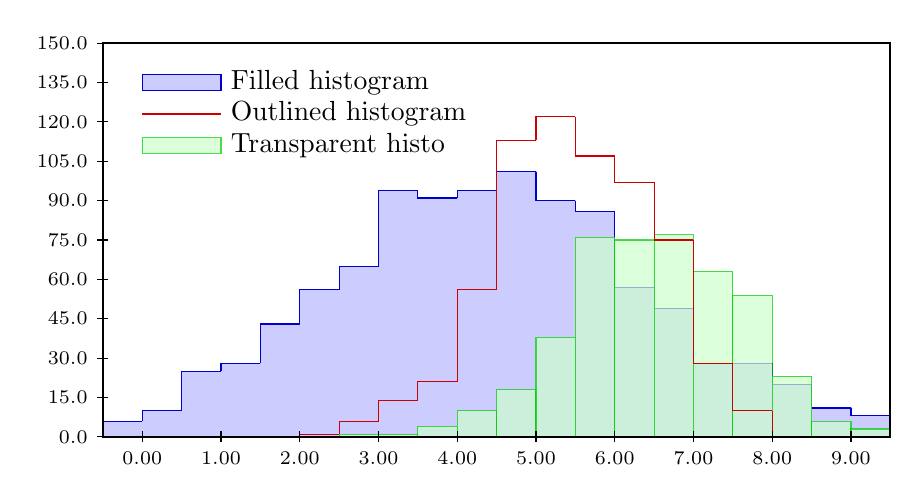
\begin{tikzpicture}
\begin{scope}[]
\clip (0,0) rectangle (10,5);
\begin{scope}[draw=blue!20,fill=blue!20]
\filldraw[] (0.0,0.0) -- (0.0,0.2) -- (0.5,0.2) -- (0.5,0.0);
\filldraw[] (0.5,0.0) -- (0.5,0.33333334) -- (1.0,0.33333334) -- (1.0,0.0);
\filldraw[] (1.0,0.0) -- (1.0,0.8333333) -- (1.5,0.8333333) -- (1.5,0.0);
\filldraw[] (1.5,0.0) -- (1.5,0.93333334) -- (2.0,0.93333334) -- (2.0,0.0);
\filldraw[] (2.0,0.0) -- (2.0,1.4333333) -- (2.5,1.4333333) -- (2.5,0.0);
\filldraw[] (2.5,0.0) -- (2.5,1.8666667) -- (3.0,1.8666667) -- (3.0,0.0);
\filldraw[] (3.0,0.0) -- (3.0,2.1666667) -- (3.5,2.1666667) -- (3.5,0.0);
\filldraw[] (3.5,0.0) -- (3.5,3.1333334) -- (4.0,3.1333334) -- (4.0,0.0);
\filldraw[] (4.0,0.0) -- (4.0,3.0333333) -- (4.5,3.0333333) -- (4.5,0.0);
\filldraw[] (4.5,0.0) -- (4.5,3.1333334) -- (5.0,3.1333334) -- (5.0,0.0);
\filldraw[] (5.0,0.0) -- (5.0,3.3666666) -- (5.5,3.3666666) -- (5.5,0.0);
\filldraw[] (5.5,0.0) -- (5.5,3.0) -- (6.0,3.0) -- (6.0,0.0);
\filldraw[] (6.0,0.0) -- (6.0,2.8666666) -- (6.5,2.8666666) -- (6.5,0.0);
\filldraw[] (6.5,0.0) -- (6.5,1.9) -- (7.0,1.9) -- (7.0,0.0);
\filldraw[] (7.0,0.0) -- (7.0,1.6333333) -- (7.5,1.6333333) -- (7.5,0.0);
\filldraw[] (7.5,0.0) -- (7.5,0.93333334) -- (8.0,0.93333334) -- (8.0,0.0);
\filldraw[] (8.0,0.0) -- (8.0,0.93333334) -- (8.5,0.93333334) -- (8.5,0.0);
\filldraw[] (8.5,0.0) -- (8.5,0.6666667) -- (9.0,0.6666667) -- (9.0,0.0);
\filldraw[] (9.0,0.0) -- (9.0,0.36666667) -- (9.5,0.36666667) -- (9.5,0.0);
\filldraw[] (9.5,0.0) -- (9.5,0.26666668) -- (10.0,0.26666668) -- (10.0,0.0);
\end{scope}
\begin{scope}[blue!80!black]
\draw[] (0.0,0.2) -- (0.5,0.2);
\draw (0.5,0.2) -- (0.5,0.33333334) -- (1.0,0.33333334);
\draw (1.0,0.33333334) -- (1.0,0.8333333) -- (1.5,0.8333333);
\draw (1.5,0.8333333) -- (1.5,0.93333334) -- (2.0,0.93333334);
\draw (2.0,0.93333334) -- (2.0,1.4333333) -- (2.5,1.4333333);
\draw (2.5,1.4333333) -- (2.5,1.8666667) -- (3.0,1.8666667);
\draw (3.0,1.8666667) -- (3.0,2.1666667) -- (3.5,2.1666667);
\draw (3.5,2.1666667) -- (3.5,3.1333334) -- (4.0,3.1333334);
\draw (4.0,3.1333334) -- (4.0,3.0333333) -- (4.5,3.0333333);
\draw (4.5,3.0333333) -- (4.5,3.1333334) -- (5.0,3.1333334);
\draw (5.0,3.1333334) -- (5.0,3.3666666) -- (5.5,3.3666666);
\draw (5.5,3.3666666) -- (5.5,3.0) -- (6.0,3.0);
\draw (6.0,3.0) -- (6.0,2.8666666) -- (6.5,2.8666666);
\draw (6.5,2.8666666) -- (6.5,1.9) -- (7.0,1.9);
\draw (7.0,1.9) -- (7.0,1.6333333) -- (7.5,1.6333333);
\draw (7.5,1.6333333) -- (7.5,0.93333334) -- (8.0,0.93333334);
\draw (8.0,0.93333334) -- (8.0,0.93333334) -- (8.5,0.93333334);
\draw (8.5,0.93333334) -- (8.5,0.6666667) -- (9.0,0.6666667);
\draw (9.0,0.6666667) -- (9.0,0.36666667) -- (9.5,0.36666667);
\draw (9.5,0.36666667) -- (9.5,0.26666668) -- (10.0,0.26666668);
\end{scope}
\begin{scope}[opacity=0.7,draw=green!80!black,fill=green!20]
\filldraw[] (0.0,0.0) -- (0.0,0.0) -- (0.5,0.0) -- (0.5,0.0);
\filldraw[] (0.5,0.0) -- (0.5,0.0) -- (1.0,0.0) -- (1.0,0.0);
\filldraw[] (1.0,0.0) -- (1.0,0.0) -- (1.5,0.0) -- (1.5,0.0);
\filldraw[] (1.5,0.0) -- (1.5,0.0) -- (2.0,0.0) -- (2.0,0.0);
\filldraw[] (2.0,0.0) -- (2.0,0.0) -- (2.5,0.0) -- (2.5,0.0);
\filldraw[] (2.5,0.0) -- (2.5,0.0) -- (3.0,0.0) -- (3.0,0.0);
\filldraw[] (3.0,0.0) -- (3.0,0.033333335) -- (3.5,0.033333335) -- (3.5,0.0);
\filldraw[] (3.5,0.0) -- (3.5,0.033333335) -- (4.0,0.033333335) -- (4.0,0.0);
\filldraw[] (4.0,0.0) -- (4.0,0.13333334) -- (4.5,0.13333334) -- (4.5,0.0);
\filldraw[] (4.5,0.0) -- (4.5,0.33333334) -- (5.0,0.33333334) -- (5.0,0.0);
\filldraw[] (5.0,0.0) -- (5.0,0.6) -- (5.5,0.6) -- (5.5,0.0);
\filldraw[] (5.5,0.0) -- (5.5,1.2666667) -- (6.0,1.2666667) -- (6.0,0.0);
\filldraw[] (6.0,0.0) -- (6.0,2.5333333) -- (6.5,2.5333333) -- (6.5,0.0);
\filldraw[] (6.5,0.0) -- (6.5,2.5) -- (7.0,2.5) -- (7.0,0.0);
\filldraw[] (7.0,0.0) -- (7.0,2.5666666) -- (7.5,2.5666666) -- (7.5,0.0);
\filldraw[] (7.5,0.0) -- (7.5,2.1) -- (8.0,2.1) -- (8.0,0.0);
\filldraw[] (8.0,0.0) -- (8.0,1.8) -- (8.5,1.8) -- (8.5,0.0);
\filldraw[] (8.5,0.0) -- (8.5,0.76666665) -- (9.0,0.76666665) -- (9.0,0.0);
\filldraw[] (9.0,0.0) -- (9.0,0.2) -- (9.5,0.2) -- (9.5,0.0);
\filldraw[] (9.5,0.0) -- (9.5,0.1) -- (10.0,0.1) -- (10.0,0.0);
\end{scope}
\begin{scope}[red!80!black]
\draw[] (0.0,0.0) -- (0.5,0.0);
\draw (0.5,0.0) -- (0.5,0.0) -- (1.0,0.0);
\draw (1.0,0.0) -- (1.0,0.0) -- (1.5,0.0);
\draw (1.5,0.0) -- (1.5,0.0) -- (2.0,0.0);
\draw (2.0,0.0) -- (2.0,0.0) -- (2.5,0.0);
\draw (2.5,0.0) -- (2.5,0.033333335) -- (3.0,0.033333335);
\draw (3.0,0.033333335) -- (3.0,0.2) -- (3.5,0.2);
\draw (3.5,0.2) -- (3.5,0.46666667) -- (4.0,0.46666667);
\draw (4.0,0.46666667) -- (4.0,0.7) -- (4.5,0.7);
\draw (4.5,0.7) -- (4.5,1.8666667) -- (5.0,1.8666667);
\draw (5.0,1.8666667) -- (5.0,3.7666667) -- (5.5,3.7666667);
\draw (5.5,3.7666667) -- (5.5,4.0666666) -- (6.0,4.0666666);
\draw (6.0,4.0666666) -- (6.0,3.5666666) -- (6.5,3.5666666);
\draw (6.5,3.5666666) -- (6.5,3.2333333) -- (7.0,3.2333333);
\draw (7.0,3.2333333) -- (7.0,2.5) -- (7.5,2.5);
\draw (7.5,2.5) -- (7.5,0.93333334) -- (8.0,0.93333334);
\draw (8.0,0.93333334) -- (8.0,0.33333334) -- (8.5,0.33333334);
\draw (8.5,0.33333334) -- (8.5,0.0) -- (9.0,0.0);
\draw (9.0,0.0) -- (9.0,0.0) -- (9.5,0.0);
\draw (9.5,0.0) -- (9.5,0.0) -- (10.0,0.0);
\end{scope}
\end{scope}
\draw (0.5,0cm + 2pt) -- (0.5, 0cm -2pt) node[below] {\scriptsize{\num[round-mode=places,round-precision=2]{0}}};
\draw (1.5,0cm + 2pt) -- (1.5, 0cm -2pt) node[below] {\scriptsize{\num[round-mode=places,round-precision=2]{1}}};
\draw (2.5,0cm + 2pt) -- (2.5, 0cm -2pt) node[below] {\scriptsize{\num[round-mode=places,round-precision=2]{2}}};
\draw (3.5,0cm + 2pt) -- (3.5, 0cm -2pt) node[below] {\scriptsize{\num[round-mode=places,round-precision=2]{3}}};
\draw (4.5,0cm + 2pt) -- (4.5, 0cm -2pt) node[below] {\scriptsize{\num[round-mode=places,round-precision=2]{4}}};
\draw (5.5,0cm + 2pt) -- (5.5, 0cm -2pt) node[below] {\scriptsize{\num[round-mode=places,round-precision=2]{5}}};
\draw (6.5,0cm + 2pt) -- (6.5, 0cm -2pt) node[below] {\scriptsize{\num[round-mode=places,round-precision=2]{6}}};
\draw (7.5,0cm + 2pt) -- (7.5, 0cm -2pt) node[below] {\scriptsize{\num[round-mode=places,round-precision=2]{7}}};
\draw (8.5,0cm + 2pt) -- (8.5, 0cm -2pt) node[below] {\scriptsize{\num[round-mode=places,round-precision=2]{8}}};
\draw (9.5,0cm + 2pt) -- (9.5, 0cm -2pt) node[below] {\scriptsize{\num[round-mode=places,round-precision=2]{9}}};
\draw (0cm + 2pt,0.    ) -- (0cm-2pt,0.    ) node[left] {\scriptsize{\num[round-mode=places,round-precision=1]{0}}};
\draw (0cm + 2pt,0.5    ) -- (0cm-2pt,0.5    ) node[left] {\scriptsize{\num[round-mode=places,round-precision=1]{15}}};
\draw (0cm + 2pt,1.    ) -- (0cm-2pt,1.    ) node[left] {\scriptsize{\num[round-mode=places,round-precision=1]{30}}};
\draw (0cm + 2pt,1.5    ) -- (0cm-2pt,1.5    ) node[left] {\scriptsize{\num[round-mode=places,round-precision=1]{45}}};
\draw (0cm + 2pt,2.    ) -- (0cm-2pt,2.    ) node[left] {\scriptsize{\num[round-mode=places,round-precision=1]{60}}};
\draw (0cm + 2pt,2.5    ) -- (0cm-2pt,2.5    ) node[left] {\scriptsize{\num[round-mode=places,round-precision=1]{75}}};
\draw (0cm + 2pt,3.    ) -- (0cm-2pt,3.    ) node[left] {\scriptsize{\num[round-mode=places,round-precision=1]{90}}};
\draw (0cm + 2pt,3.5    ) -- (0cm-2pt,3.5    ) node[left] {\scriptsize{\num[round-mode=places,round-precision=1]{105}}};
\draw (0cm + 2pt,4.    ) -- (0cm-2pt,4.    ) node[left] {\scriptsize{\num[round-mode=places,round-precision=1]{120}}};
\draw (0cm + 2pt,4.5    ) -- (0cm-2pt,4.5    ) node[left] {\scriptsize{\num[round-mode=places,round-precision=1]{135}}};
\draw (0cm + 2pt,5.    ) -- (0cm-2pt,5.    ) node[left] {\scriptsize{\num[round-mode=places,round-precision=1]{150}}};
\draw[thick] (0,0) rectangle (10,5);
\draw[draw=blue!20,fill=blue!20] (0.5,4.4) rectangle (1.5,4.6);
\draw[blue!80!black] (0.5,4.4) rectangle (1.5,4.6);
\node[right,] at (1.5,4.5) {Filled histogram};
\draw[red!80!black] (0.5,4.1) -- (1.5,4.1);
\node[right,] at (1.5,4.1) {Outlined histogram};
\draw[opacity=0.7,draw=green!80!black,fill=green!20] (0.5,3.6000001) rectangle (1.5,3.8);
\node[right,] at (1.5,3.7) {Transparent histo};
\end{tikzpicture}
%%% Local Variables: 
%%% mode: latex 
%%% TeX-master: "master" 
%%% End:


\captionsetup{singlelinecheck=off}
\caption[asdf]{Some Gaussian histograms with different styles and with legend entries. 
The legend entries are placed in the default cm frame, unless draw-histogram 
is called within (transform (tikz) ...). With some trickery it is also possible to get 
legends in captions: 
\begin{tikzpicture}
\node at (0.2,0.1) [draw=gray,fill=blue!50,rectangle,inner sep=0.0cm,minimum width =0.4cm,minimum height=0.2cm] {};
\end{tikzpicture}
 Histogram 1, \begin{tikzpicture}
\draw[red!80,thick] (0.0,0.1) -- (0.4,0.1);
\draw[opacity=0.0,white] (0.0,0.2) -- (0.0,0.0);
\end{tikzpicture}
 Hisogram 2, 
\begin{tikzpicture}
\node at (0.2,0.1) [fill=green,rectangle,inner sep=0.0cm,minimum width =0.4cm,minimum height=0.2cm] {};
\end{tikzpicture}
 Hisogram 3.}
\end{figure}
\begin{figure}[H]
\centering
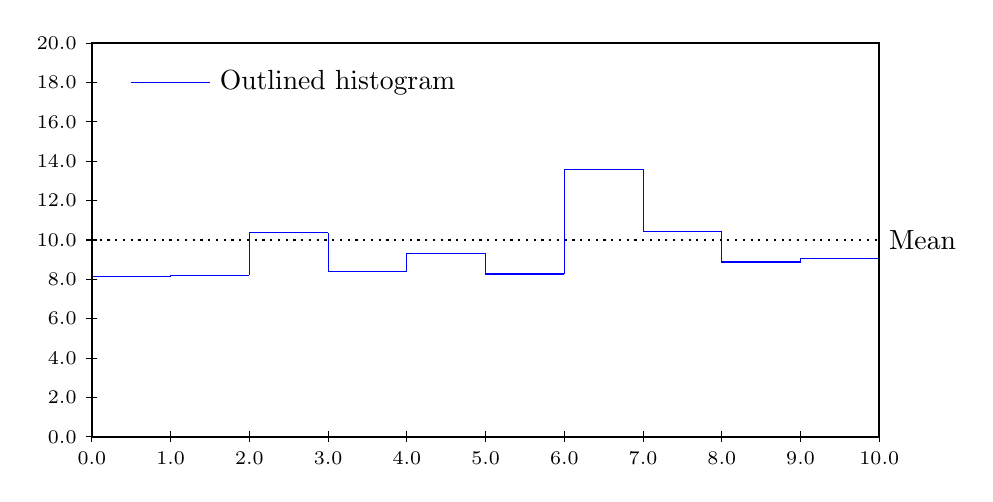
\begin{tikzpicture}
\begin{scope}[]
\clip (0,0) rectangle (10,5);
\begin{scope}[blue]
\draw[] (0.0,2.040753989729346) -- (1.0,2.040753989729346);
\draw (1.0,2.040753989729346) -- (1.0,2.0520371396851527) -- (2.0,2.0520371396851527);
\draw (2.0,2.0520371396851527) -- (2.0,2.589490136587087) -- (3.0,2.589490136587087);
\draw (3.0,2.589490136587087) -- (3.0,2.10531930397396) -- (4.0,2.10531930397396);
\draw (4.0,2.10531930397396) -- (4.0,2.328047479221825) -- (5.0,2.328047479221825);
\draw (5.0,2.328047479221825) -- (5.0,2.067390163042384) -- (6.0,2.067390163042384);
\draw (6.0,2.067390163042384) -- (6.0,3.3961419895360887) -- (7.0,3.3961419895360887);
\draw (7.0,3.3961419895360887) -- (7.0,2.6085288458106475) -- (8.0,2.6085288458106475);
\draw (8.0,2.6085288458106475) -- (8.0,2.2210174657245827) -- (9.0,2.2210174657245827);
\draw (9.0,2.2210174657245827) -- (9.0,2.2670683657782047) -- (10.0,2.2670683657782047);
\end{scope}
\end{scope}
\draw (0,0cm + 2pt) -- (0, 0cm -2pt) node[below] {\scriptsize{\num[round-mode=places,round-precision=1]{0}}};
\draw (1,0cm + 2pt) -- (1, 0cm -2pt) node[below] {\scriptsize{\num[round-mode=places,round-precision=1]{1}}};
\draw (2,0cm + 2pt) -- (2, 0cm -2pt) node[below] {\scriptsize{\num[round-mode=places,round-precision=1]{2}}};
\draw (3,0cm + 2pt) -- (3, 0cm -2pt) node[below] {\scriptsize{\num[round-mode=places,round-precision=1]{3}}};
\draw (4,0cm + 2pt) -- (4, 0cm -2pt) node[below] {\scriptsize{\num[round-mode=places,round-precision=1]{4}}};
\draw (5,0cm + 2pt) -- (5, 0cm -2pt) node[below] {\scriptsize{\num[round-mode=places,round-precision=1]{5}}};
\draw (6,0cm + 2pt) -- (6, 0cm -2pt) node[below] {\scriptsize{\num[round-mode=places,round-precision=1]{6}}};
\draw (7,0cm + 2pt) -- (7, 0cm -2pt) node[below] {\scriptsize{\num[round-mode=places,round-precision=1]{7}}};
\draw (8,0cm + 2pt) -- (8, 0cm -2pt) node[below] {\scriptsize{\num[round-mode=places,round-precision=1]{8}}};
\draw (9,0cm + 2pt) -- (9, 0cm -2pt) node[below] {\scriptsize{\num[round-mode=places,round-precision=1]{9}}};
\draw (10,0cm + 2pt) -- (10, 0cm -2pt) node[below] {\scriptsize{\num[round-mode=places,round-precision=1]{10}}};
\draw (0cm + 2pt,0.    ) -- (0cm-2pt,0.    ) node[left] {\scriptsize{\num[round-mode=places,round-precision=1]{0}}};
\draw (0cm + 2pt,0.5    ) -- (0cm-2pt,0.5    ) node[left] {\scriptsize{\num[round-mode=places,round-precision=1]{2}}};
\draw (0cm + 2pt,1.    ) -- (0cm-2pt,1.    ) node[left] {\scriptsize{\num[round-mode=places,round-precision=1]{4}}};
\draw (0cm + 2pt,1.5    ) -- (0cm-2pt,1.5    ) node[left] {\scriptsize{\num[round-mode=places,round-precision=1]{6}}};
\draw (0cm + 2pt,2.    ) -- (0cm-2pt,2.    ) node[left] {\scriptsize{\num[round-mode=places,round-precision=1]{8}}};
\draw (0cm + 2pt,2.5    ) -- (0cm-2pt,2.5    ) node[left] {\scriptsize{\num[round-mode=places,round-precision=1]{10}}};
\draw (0cm + 2pt,3.    ) -- (0cm-2pt,3.    ) node[left] {\scriptsize{\num[round-mode=places,round-precision=1]{12}}};
\draw (0cm + 2pt,3.5    ) -- (0cm-2pt,3.5    ) node[left] {\scriptsize{\num[round-mode=places,round-precision=1]{14}}};
\draw (0cm + 2pt,4.    ) -- (0cm-2pt,4.    ) node[left] {\scriptsize{\num[round-mode=places,round-precision=1]{16}}};
\draw (0cm + 2pt,4.5    ) -- (0cm-2pt,4.5    ) node[left] {\scriptsize{\num[round-mode=places,round-precision=1]{18}}};
\draw (0cm + 2pt,5.    ) -- (0cm-2pt,5.    ) node[left] {\scriptsize{\num[round-mode=places,round-precision=1]{20}}};
\draw[thick] (0,0) rectangle (10,5);
\draw[thick,dotted] (0.0,2.5) -- (10.0,2.5);
\node[right] at (10.0,2.5) {Mean};
\draw[blue] (0.5,4.5) -- (1.5,4.5);
\node[right,] at (1.5,4.5) {Outlined histogram};
\end{tikzpicture}
%%% Local Variables: 
%%% mode: latex 
%%% TeX-master: "master" 
%%% End:


\captionsetup{singlelinecheck=off}
\caption[asdf]{Histogram with bins extending in the horizontal direction. 
The bins are named with the draw-axis-ticks function.}
\end{figure}
\begin{figure}[H]
\centering
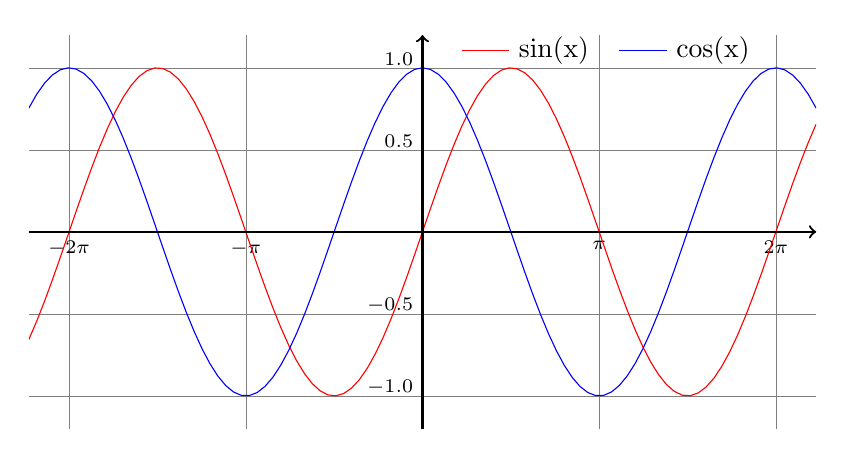
\begin{tikzpicture}[]
\begin{scope}[]
\clip (0.0,0.0) rectangle (10.0,5.0);
\begin{scope}[shift={(0.0,0.0)}]
\pgfsetxvec{\pgfpoint{0.71428573cm}{0cm}}
\pgfsetyvec{\pgfpoint{0cm}{2.0833333cm}}
\begin{scope}[shift={(7.0,1.2)}]
\begin{scope}[yshift=2.5cm]
\draw[ultra thin,gray] [shift={(-6.283185307179586,-1.2)}] (0,2.5cm) -- (0,-2.5cm) node[black,midway,below]{ \scriptsize{$-2\pi$}};
\draw[ultra thin,gray] [shift={(-3.141592653589793,-1.2)}] (0,2.5cm) -- (0,-2.5cm) node[black,midway,below]{ \scriptsize{$-\pi$}};
\draw[ultra thin,gray] [shift={(3.141592653589793,-1.2)}] (0,2.5cm) -- (0,-2.5cm) node[black,midway,below]{ \scriptsize{$\pi$}};
\draw[ultra thin,gray] [shift={(6.283185307179586,-1.2)}] (0,2.5cm) -- (0,-2.5cm) node[black,midway,below]{ \scriptsize{$2\pi$}};
\end{scope}
\begin{scope}[xshift=5cm]
\draw[ultra thin,gray] [shift={(-7.0,-1.0)}] (5cm,0) -- (-5cm,0) node[above=3pt,black,midway,left]{ \scriptsize{\num[round-mode=places,round-precision=1]{-1.0}}};
\draw[ultra thin,gray] [shift={(-7.0,-0.5)}] (5cm,0) -- (-5cm,0) node[above=3pt,black,midway,left]{ \scriptsize{\num[round-mode=places,round-precision=1]{-0.5}}};
\draw[ultra thin,gray] [shift={(-7.0,0.5)}] (5cm,0) -- (-5cm,0) node[above=3pt,black,midway,left]{ \scriptsize{\num[round-mode=places,round-precision=1]{0.5}}};
\draw[ultra thin,gray] [shift={(-7.0,1.0)}] (5cm,0) -- (-5cm,0) node[above=3pt,black,midway,left]{ \scriptsize{\num[round-mode=places,round-precision=1]{1.0}}};
\end{scope}
\begin{scope}[red]
\pgfpathmoveto{ \pgfqpointxy {-7.0} {-0.6569866}}
\pgfpathlineto{ \pgfqpointxy {-6.86} {-0.54535675}}
\pgfpathlineto{ \pgfqpointxy {-6.72} {-0.4230554}}
\pgfpathlineto{ \pgfqpointxy {-6.58} {-0.29247567}}
\pgfpathlineto{ \pgfqpointxy {-6.44} {-0.15617278}}
\pgfpathlineto{ \pgfqpointxy {-6.3} {-0.0168139}}
\pgfpathlineto{ \pgfqpointxy {-6.16} {0.12287399}}
\pgfpathlineto{ \pgfqpointxy {-6.02} {0.2601575}}
\pgfpathlineto{ \pgfqpointxy {-5.88} {0.39235023}}
\pgfpathlineto{ \pgfqpointxy {-5.74} {0.51686543}}
\pgfpathlineto{ \pgfqpointxy {-5.6} {0.63126665}}
\pgfpathlineto{ \pgfqpointxy {-5.46} {0.7333152}}
\pgfpathlineto{ \pgfqpointxy {-5.32} {0.8210142}}
\pgfpathlineto{ \pgfqpointxy {-5.18} {0.8926477}}
\pgfpathlineto{ \pgfqpointxy {-5.04} {0.94681376}}
\pgfpathlineto{ \pgfqpointxy {-4.9} {0.98245263}}
\pgfpathlineto{ \pgfqpointxy {-4.76} {0.9988668}}
\pgfpathlineto{ \pgfqpointxy {-4.62} {0.99573517}}
\pgfpathlineto{ \pgfqpointxy {-4.48} {0.97311896}}
\pgfpathlineto{ \pgfqpointxy {-4.34} {0.9314608}}
\pgfpathlineto{ \pgfqpointxy {-4.2} {0.8715758}}
\pgfpathlineto{ \pgfqpointxy {-4.06} {0.7946358}}
\pgfpathlineto{ \pgfqpointxy {-3.92} {0.7021463}}
\pgfpathlineto{ \pgfqpointxy {-3.78} {0.5959172}}
\pgfpathlineto{ \pgfqpointxy {-3.64} {0.47802725}}
\pgfpathlineto{ \pgfqpointxy {-3.5} {0.35078323}}
\pgfpathlineto{ \pgfqpointxy {-3.36} {0.21667509}}
\pgfpathlineto{ \pgfqpointxy {-3.22} {0.07832703}}
\pgfpathlineto{ \pgfqpointxy {-3.08} {-0.061553717}}
\pgfpathlineto{ \pgfqpointxy {-2.94} {-0.20022999}}
\pgfpathlineto{ \pgfqpointxy {-2.8} {-0.33498815}}
\pgfpathlineto{ \pgfqpointxy {-2.66} {-0.46319127}}
\pgfpathlineto{ \pgfqpointxy {-2.52} {-0.58233064}}
\pgfpathlineto{ \pgfqpointxy {-2.38} {-0.690075}}
\pgfpathlineto{ \pgfqpointxy {-2.24} {-0.78431594}}
\pgfpathlineto{ \pgfqpointxy {-2.1} {-0.86320937}}
\pgfpathlineto{ \pgfqpointxy {-1.96} {-0.92521155}}
\pgfpathlineto{ \pgfqpointxy {-1.82} {-0.9691091}}
\pgfpathlineto{ \pgfqpointxy {-1.68} {-0.99404323}}
\pgfpathlineto{ \pgfqpointxy {-1.54} {-0.99952585}}
\pgfpathlineto{ \pgfqpointxy {-1.4} {-0.98544973}}
\pgfpathlineto{ \pgfqpointxy {-1.26} {-0.9520903}}
\pgfpathlineto{ \pgfqpointxy {-1.12} {-0.90010047}}
\pgfpathlineto{ \pgfqpointxy {-0.98} {-0.8304974}}
\pgfpathlineto{ \pgfqpointxy {-0.84} {-0.7446431}}
\pgfpathlineto{ \pgfqpointxy {-0.7} {-0.64421767}}
\pgfpathlineto{ \pgfqpointxy {-0.56} {-0.5311862}}
\pgfpathlineto{ \pgfqpointxy {-0.42} {-0.40776044}}
\pgfpathlineto{ \pgfqpointxy {-0.28} {-0.27635565}}
\pgfpathlineto{ \pgfqpointxy {-0.14} {-0.13954312}}
\pgfpathlineto{ \pgfqpointxy {0.0} {0.0}}
\pgfpathlineto{ \pgfqpointxy {0.14} {0.13954312}}
\pgfpathlineto{ \pgfqpointxy {0.28} {0.27635565}}
\pgfpathlineto{ \pgfqpointxy {0.42} {0.40776044}}
\pgfpathlineto{ \pgfqpointxy {0.56} {0.5311862}}
\pgfpathlineto{ \pgfqpointxy {0.7} {0.64421767}}
\pgfpathlineto{ \pgfqpointxy {0.84} {0.7446431}}
\pgfpathlineto{ \pgfqpointxy {0.98} {0.8304974}}
\pgfpathlineto{ \pgfqpointxy {1.12} {0.90010047}}
\pgfpathlineto{ \pgfqpointxy {1.26} {0.9520903}}
\pgfpathlineto{ \pgfqpointxy {1.4} {0.98544973}}
\pgfpathlineto{ \pgfqpointxy {1.54} {0.99952585}}
\pgfpathlineto{ \pgfqpointxy {1.68} {0.99404323}}
\pgfpathlineto{ \pgfqpointxy {1.82} {0.9691091}}
\pgfpathlineto{ \pgfqpointxy {1.96} {0.92521155}}
\pgfpathlineto{ \pgfqpointxy {2.1} {0.86320937}}
\pgfpathlineto{ \pgfqpointxy {2.24} {0.78431594}}
\pgfpathlineto{ \pgfqpointxy {2.38} {0.690075}}
\pgfpathlineto{ \pgfqpointxy {2.52} {0.58233064}}
\pgfpathlineto{ \pgfqpointxy {2.66} {0.46319127}}
\pgfpathlineto{ \pgfqpointxy {2.8} {0.33498815}}
\pgfpathlineto{ \pgfqpointxy {2.94} {0.20022999}}
\pgfpathlineto{ \pgfqpointxy {3.08} {0.061553717}}
\pgfpathlineto{ \pgfqpointxy {3.22} {-0.07832703}}
\pgfpathlineto{ \pgfqpointxy {3.36} {-0.21667509}}
\pgfpathlineto{ \pgfqpointxy {3.5} {-0.35078323}}
\pgfpathlineto{ \pgfqpointxy {3.64} {-0.47802725}}
\pgfpathlineto{ \pgfqpointxy {3.78} {-0.5959172}}
\pgfpathlineto{ \pgfqpointxy {3.92} {-0.7021463}}
\pgfpathlineto{ \pgfqpointxy {4.06} {-0.7946358}}
\pgfpathlineto{ \pgfqpointxy {4.2} {-0.8715758}}
\pgfpathlineto{ \pgfqpointxy {4.34} {-0.9314608}}
\pgfpathlineto{ \pgfqpointxy {4.48} {-0.97311896}}
\pgfpathlineto{ \pgfqpointxy {4.62} {-0.99573517}}
\pgfpathlineto{ \pgfqpointxy {4.76} {-0.9988668}}
\pgfpathlineto{ \pgfqpointxy {4.9} {-0.98245263}}
\pgfpathlineto{ \pgfqpointxy {5.04} {-0.94681376}}
\pgfpathlineto{ \pgfqpointxy {5.18} {-0.8926477}}
\pgfpathlineto{ \pgfqpointxy {5.32} {-0.8210142}}
\pgfpathlineto{ \pgfqpointxy {5.46} {-0.7333152}}
\pgfpathlineto{ \pgfqpointxy {5.6} {-0.63126665}}
\pgfpathlineto{ \pgfqpointxy {5.74} {-0.51686543}}
\pgfpathlineto{ \pgfqpointxy {5.88} {-0.39235023}}
\pgfpathlineto{ \pgfqpointxy {6.02} {-0.2601575}}
\pgfpathlineto{ \pgfqpointxy {6.16} {-0.12287399}}
\pgfpathlineto{ \pgfqpointxy {6.3} {0.0168139}}
\pgfpathlineto{ \pgfqpointxy {6.44} {0.15617278}}
\pgfpathlineto{ \pgfqpointxy {6.58} {0.29247567}}
\pgfpathlineto{ \pgfqpointxy {6.72} {0.4230554}}
\pgfpathlineto{ \pgfqpointxy {6.86} {0.54535675}}
\pgfpathlineto{ \pgfqpointxy {7.0} {0.6569866}}
\pgfusepath{ stroke }
\end{scope}
\begin{scope}[blue]
\pgfpathmoveto{ \pgfqpointxy {-7.0} {0.75390226}}
\pgfpathlineto{ \pgfqpointxy {-6.86} {0.838204}}
\pgfpathlineto{ \pgfqpointxy {-6.72} {0.9061038}}
\pgfpathlineto{ \pgfqpointxy {-6.58} {0.95627296}}
\pgfpathlineto{ \pgfqpointxy {-6.44} {0.9877297}}
\pgfpathlineto{ \pgfqpointxy {-6.3} {0.9998586}}
\pgfpathlineto{ \pgfqpointxy {-6.16} {0.9924223}}
\pgfpathlineto{ \pgfqpointxy {-6.02} {0.9655662}}
\pgfpathlineto{ \pgfqpointxy {-5.88} {0.9198159}}
\pgfpathlineto{ \pgfqpointxy {-5.74} {0.85606664}}
\pgfpathlineto{ \pgfqpointxy {-5.6} {0.77556586}}
\pgfpathlineto{ \pgfqpointxy {-5.46} {0.67988884}}
\pgfpathlineto{ \pgfqpointxy {-5.32} {0.5709077}}
\pgfpathlineto{ \pgfqpointxy {-5.18} {0.45075506}}
\pgfpathlineto{ \pgfqpointxy {-5.04} {0.32178202}}
\pgfpathlineto{ \pgfqpointxy {-4.9} {0.18651237}}
\pgfpathlineto{ \pgfqpointxy {-4.76} {0.047593035}}
\pgfpathlineto{ \pgfqpointxy {-4.62} {-0.092257604}}
\pgfpathlineto{ \pgfqpointxy {-4.48} {-0.23030294}}
\pgfpathlineto{ \pgfqpointxy {-4.34} {-0.3638417}}
\pgfpathlineto{ \pgfqpointxy {-4.2} {-0.4902608}}
\pgfpathlineto{ \pgfqpointxy {-4.06} {-0.6070865}}
\pgfpathlineto{ \pgfqpointxy {-3.92} {-0.71203274}}
\pgfpathlineto{ \pgfqpointxy {-3.78} {-0.80304587}}
\pgfpathlineto{ \pgfqpointxy {-3.64} {-0.878345}}
\pgfpathlineto{ \pgfqpointxy {-3.5} {-0.9364567}}
\pgfpathlineto{ \pgfqpointxy {-3.36} {-0.9762438}}
\pgfpathlineto{ \pgfqpointxy {-3.22} {-0.99692774}}
\pgfpathlineto{ \pgfqpointxy {-3.08} {-0.9981038}}
\pgfpathlineto{ \pgfqpointxy {-2.94} {-0.9797489}}
\pgfpathlineto{ \pgfqpointxy {-2.8} {-0.94222236}}
\pgfpathlineto{ \pgfqpointxy {-2.66} {-0.88625836}}
\pgfpathlineto{ \pgfqpointxy {-2.52} {-0.81295204}}
\pgfpathlineto{ \pgfqpointxy {-2.38} {-0.7237379}}
\pgfpathlineto{ \pgfqpointxy {-2.24} {-0.6203616}}
\pgfpathlineto{ \pgfqpointxy {-2.1} {-0.5048461}}
\pgfpathlineto{ \pgfqpointxy {-1.96} {-0.37945175}}
\pgfpathlineto{ \pgfqpointxy {-1.82} {-0.24663231}}
\pgfpathlineto{ \pgfqpointxy {-1.68} {-0.10898675}}
\pgfpathlineto{ \pgfqpointxy {-1.54} {0.03079146}}
\pgfpathlineto{ \pgfqpointxy {-1.4} {0.16996714}}
\pgfpathlineto{ \pgfqpointxy {-1.26} {0.30581692}}
\pgfpathlineto{ \pgfqpointxy {-1.12} {0.43568245}}
\pgfpathlineto{ \pgfqpointxy {-0.98} {0.5570226}}
\pgfpathlineto{ \pgfqpointxy {-0.84} {0.6674628}}
\pgfpathlineto{ \pgfqpointxy {-0.7} {0.7648422}}
\pgfpathlineto{ \pgfqpointxy {-0.56} {0.8472551}}
\pgfpathlineto{ \pgfqpointxy {-0.42} {0.9130889}}
\pgfpathlineto{ \pgfqpointxy {-0.28} {0.96105546}}
\pgfpathlineto{ \pgfqpointxy {-0.14} {0.990216}}
\pgfpathlineto{ \pgfqpointxy {0.0} {1.0}}
\pgfpathlineto{ \pgfqpointxy {0.14} {0.990216}}
\pgfpathlineto{ \pgfqpointxy {0.28} {0.96105546}}
\pgfpathlineto{ \pgfqpointxy {0.42} {0.9130889}}
\pgfpathlineto{ \pgfqpointxy {0.56} {0.8472551}}
\pgfpathlineto{ \pgfqpointxy {0.7} {0.7648422}}
\pgfpathlineto{ \pgfqpointxy {0.84} {0.6674628}}
\pgfpathlineto{ \pgfqpointxy {0.98} {0.5570226}}
\pgfpathlineto{ \pgfqpointxy {1.12} {0.43568245}}
\pgfpathlineto{ \pgfqpointxy {1.26} {0.30581692}}
\pgfpathlineto{ \pgfqpointxy {1.4} {0.16996714}}
\pgfpathlineto{ \pgfqpointxy {1.54} {0.03079146}}
\pgfpathlineto{ \pgfqpointxy {1.68} {-0.10898675}}
\pgfpathlineto{ \pgfqpointxy {1.82} {-0.24663231}}
\pgfpathlineto{ \pgfqpointxy {1.96} {-0.37945175}}
\pgfpathlineto{ \pgfqpointxy {2.1} {-0.5048461}}
\pgfpathlineto{ \pgfqpointxy {2.24} {-0.6203616}}
\pgfpathlineto{ \pgfqpointxy {2.38} {-0.7237379}}
\pgfpathlineto{ \pgfqpointxy {2.52} {-0.81295204}}
\pgfpathlineto{ \pgfqpointxy {2.66} {-0.88625836}}
\pgfpathlineto{ \pgfqpointxy {2.8} {-0.94222236}}
\pgfpathlineto{ \pgfqpointxy {2.94} {-0.9797489}}
\pgfpathlineto{ \pgfqpointxy {3.08} {-0.9981038}}
\pgfpathlineto{ \pgfqpointxy {3.22} {-0.99692774}}
\pgfpathlineto{ \pgfqpointxy {3.36} {-0.9762438}}
\pgfpathlineto{ \pgfqpointxy {3.5} {-0.9364567}}
\pgfpathlineto{ \pgfqpointxy {3.64} {-0.878345}}
\pgfpathlineto{ \pgfqpointxy {3.78} {-0.80304587}}
\pgfpathlineto{ \pgfqpointxy {3.92} {-0.71203274}}
\pgfpathlineto{ \pgfqpointxy {4.06} {-0.6070865}}
\pgfpathlineto{ \pgfqpointxy {4.2} {-0.4902608}}
\pgfpathlineto{ \pgfqpointxy {4.34} {-0.3638417}}
\pgfpathlineto{ \pgfqpointxy {4.48} {-0.23030294}}
\pgfpathlineto{ \pgfqpointxy {4.62} {-0.092257604}}
\pgfpathlineto{ \pgfqpointxy {4.76} {0.047593035}}
\pgfpathlineto{ \pgfqpointxy {4.9} {0.18651237}}
\pgfpathlineto{ \pgfqpointxy {5.04} {0.32178202}}
\pgfpathlineto{ \pgfqpointxy {5.18} {0.45075506}}
\pgfpathlineto{ \pgfqpointxy {5.32} {0.5709077}}
\pgfpathlineto{ \pgfqpointxy {5.46} {0.67988884}}
\pgfpathlineto{ \pgfqpointxy {5.6} {0.77556586}}
\pgfpathlineto{ \pgfqpointxy {5.74} {0.85606664}}
\pgfpathlineto{ \pgfqpointxy {5.88} {0.9198159}}
\pgfpathlineto{ \pgfqpointxy {6.02} {0.9655662}}
\pgfpathlineto{ \pgfqpointxy {6.16} {0.9924223}}
\pgfpathlineto{ \pgfqpointxy {6.3} {0.9998586}}
\pgfpathlineto{ \pgfqpointxy {6.44} {0.9877297}}
\pgfpathlineto{ \pgfqpointxy {6.58} {0.95627296}}
\pgfpathlineto{ \pgfqpointxy {6.72} {0.9061038}}
\pgfpathlineto{ \pgfqpointxy {6.86} {0.838204}}
\pgfpathlineto{ \pgfqpointxy {7.0} {0.75390226}}
\pgfusepath{ stroke }
\end{scope}
\end{scope}
\pgfsetxvec{\pgfpoint{1cm}{0cm}}
\pgfsetyvec{\pgfpoint{0cm}{1cm}}
\end{scope}
\end{scope}
\draw[thick,->] (5.0,0.0) -- (5.0,5.0);
\draw[thick,->] (0.0,2.5) -- (10.0,2.5);
\draw[red] (5.5,4.8) -- (6.1,4.8);
\node[right,] at (6.1,4.8) {sin(x)};
\draw[blue] (7.5,4.8) -- (8.1,4.8);
\node[right,] at (8.1,4.8) {cos(x)};
\end{tikzpicture}
%%% Local Variables: 
%%% mode: latex 
%%% TeX-master: "master" 
%%% End:


\captionsetup{singlelinecheck=off}
\caption[asdf]{Plotting sin(x) and cos(x), with grid lines and tick names on the x-axis.}
\end{figure}
\begin{figure}[H]
\centering
\documentclass{standalone}
\ifx\HCode\UnDef\else\def\pgfsysdriver{pgfsys-tex4ht.def}\fi
\usepackage{tikz}
\usepackage{color}
\usepackage{siunitx}
\usetikzlibrary{arrows,shapes}
\begin{document}
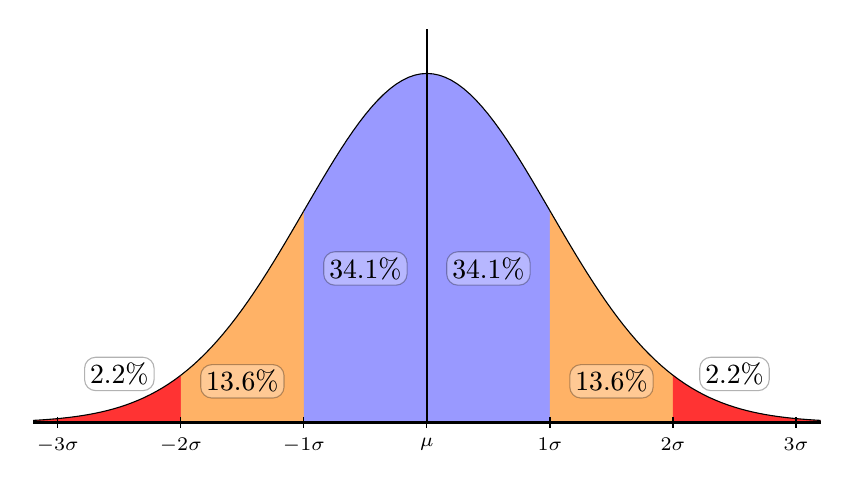
\begin{tikzpicture}
\begin{scope}[]
\pgfpathmoveto{ \pgfpointxy {0.0} {0.0}}
\pgfpathlineto{ \pgfpointxy {10.0} {0.0}}
\pgfpathlineto{ \pgfpointxy {10.0} {5.0}}
\pgfpathlineto{ \pgfpointxy {0.0} {5.0}}
\pgfpathclose
\pgfusepath{  clip, }
\begin{scope}[shift={(0.0,0.0)}]
\pgfsetxvec{\pgfpoint{1.5625cm}{0cm}}
\pgfsetyvec{\pgfpoint{0cm}{11.111112cm}}
\begin{scope}[shift={(3.2,0.0)}]
\begin{scope}[]
\pgfpathmoveto{ \pgfpointxy {-3.5} {0.0}}
\pgfpathlineto{ \pgfpointxy {-2.0} {0.0}}
\pgfpathlineto{ \pgfpointxy {-2.0} {5.0}}
\pgfpathlineto{ \pgfpointxy {-3.5} {5.0}}
\pgfpathclose
\pgfusepath{  clip, }
\begin{scope}[fill=red!80]
\pgfpathmoveto{ \pgfpointxy {-3.2} {0.0}}
\pgfpathlineto{ \pgfpointxy {-3.2} {0.0023840873753184963}}
\pgfpathlineto{ \pgfpointxy {-3.15} {0.002794257593560257}}
\pgfpathlineto{ \pgfpointxy {-3.1000001} {0.0032668180294884892}}
\pgfpathlineto{ \pgfpointxy {-3.05} {0.0038097626369961333}}
\pgfpathlineto{ \pgfpointxy {-3.0} {0.004431848335480958}}
\pgfpathlineto{ \pgfpointxy {-2.95} {0.005142640152435692}}
\pgfpathlineto{ \pgfpointxy {-2.9} {0.0059525301721895674}}
\pgfpathlineto{ \pgfpointxy {-2.8500001} {0.006872765030160735}}
\pgfpathlineto{ \pgfpointxy {-2.8} {0.007915452600647405}}
\pgfpathlineto{ \pgfpointxy {-2.75} {0.009093562739915748}}
\pgfpathlineto{ \pgfpointxy {-2.7} {0.010420932487815211}}
\pgfpathlineto{ \pgfpointxy {-2.65} {0.011912240802789813}}
\pgfpathlineto{ \pgfpointxy {-2.6} {0.013582973636746678}}
\pgfpathlineto{ \pgfpointxy {-2.55} {0.0154493503693536}}
\pgfpathlineto{ \pgfpointxy {-2.5} {0.017528300772314036}}
\pgfpathlineto{ \pgfpointxy {-2.45} {0.01983735428926949}}
\pgfpathlineto{ \pgfpointxy {-2.4} {0.022394527829526112}}
\pgfpathlineto{ \pgfpointxy {-2.35} {0.02521822470809983}}
\pgfpathlineto{ \pgfpointxy {-2.3} {0.028327036984334027}}
\pgfpathlineto{ \pgfpointxy {-2.25} {0.03173965331899954}}
\pgfpathlineto{ \pgfpointxy {-2.2} {0.03547459146264942}}
\pgfpathlineto{ \pgfpointxy {-2.15} {0.03955003329010437}}
\pgfpathlineto{ \pgfpointxy {-2.1} {0.043983610791136565}}
\pgfpathlineto{ \pgfpointxy {-2.0500002} {0.0487919988582986}}
\pgfpathlineto{ \pgfpointxy {-2.0} {0.05399096581690089}}
\pgfpathlineto{ \pgfpointxy {-1.95} {0.059594698701195395}}
\pgfpathlineto{ \pgfpointxy {-1.9} {0.0656158210884853}}
\pgfpathlineto{ \pgfpointxy {-1.85} {0.07206486699288937}}
\pgfpathlineto{ \pgfpointxy {-1.8000001} {0.07895014710951938}}
\pgfpathlineto{ \pgfpointxy {-1.75} {0.08627732079584774}}
\pgfpathlineto{ \pgfpointxy {-1.7} {0.09404907505773316}}
\pgfpathlineto{ \pgfpointxy {-1.65} {0.10226493431891748}}
\pgfpathlineto{ \pgfpointxy {-1.6} {0.11092082645768998}}
\pgfpathlineto{ \pgfpointxy {-1.5500001} {0.12000899363633905}}
\pgfpathlineto{ \pgfpointxy {-1.5} {0.12951759400603588}}
\pgfpathlineto{ \pgfpointxy {-1.45} {0.13943055308925387}}
\pgfpathlineto{ \pgfpointxy {-1.4} {0.1497274686645169}}
\pgfpathlineto{ \pgfpointxy {-1.35} {0.16038331353123803}}
\pgfpathlineto{ \pgfpointxy {-1.3000001} {0.1713685781825969}}
\pgfpathlineto{ \pgfpointxy {-1.25} {0.18264908057503657}}
\pgfpathlineto{ \pgfpointxy {-1.2} {0.19418604935410852}}
\pgfpathlineto{ \pgfpointxy {-1.1500001} {0.20593624274853736}}
\pgfpathlineto{ \pgfpointxy {-1.0999999} {0.2178522101371628}}
\pgfpathlineto{ \pgfpointxy {-1.05} {0.22988214937606208}}
\pgfpathlineto{ \pgfpointxy {-1.0} {0.24197072716759546}}
\pgfpathlineto{ \pgfpointxy {-0.95000005} {0.2540590433921869}}
\pgfpathlineto{ \pgfpointxy {-0.9000001} {0.2660852255786465}}
\pgfpathlineto{ \pgfpointxy {-0.8499999} {0.2779849044804291}}
\pgfpathlineto{ \pgfpointxy {-0.79999995} {0.28969157075782764}}
\pgfpathlineto{ \pgfpointxy {-0.75} {0.301137431015238}}
\pgfpathlineto{ \pgfpointxy {-0.70000005} {0.3122539309350428}}
\pgfpathlineto{ \pgfpointxy {-0.6500001} {0.3229723497479345}}
\pgfpathlineto{ \pgfpointxy {-0.5999999} {0.33322460871255405}}
\pgfpathlineto{ \pgfpointxy {-0.54999995} {0.3429438655858136}}
\pgfpathlineto{ \pgfpointxy {-0.5} {0.3520653231025355}}
\pgfpathlineto{ \pgfpointxy {-0.45000005} {0.3605269661186527}}
\pgfpathlineto{ \pgfpointxy {-0.4000001} {0.368270132302718}}
\pgfpathlineto{ \pgfpointxy {-0.3499999} {0.3752403681731694}}
\pgfpathlineto{ \pgfpointxy {-0.29999995} {0.38138780955933627}}
\pgfpathlineto{ \pgfpointxy {-0.25} {0.3866681089751429}}
\pgfpathlineto{ \pgfpointxy {-0.20000005} {0.39104269718605056}}
\pgfpathlineto{ \pgfpointxy {-0.1500001} {0.3944793301217544}}
\pgfpathlineto{ \pgfpointxy {-0.099999905} {0.3969525406736286}}
\pgfpathlineto{ \pgfpointxy {-0.049999952} {0.39844392404048146}}
\pgfpathlineto{ \pgfpointxy {0.0} {0.3989422804014327}}
\pgfpathlineto{ \pgfpointxy {0.049999952} {0.39844392404048146}}
\pgfpathlineto{ \pgfpointxy {0.099999905} {0.3969525406736286}}
\pgfpathlineto{ \pgfpointxy {0.1500001} {0.3944793301217544}}
\pgfpathlineto{ \pgfpointxy {0.20000005} {0.39104269718605056}}
\pgfpathlineto{ \pgfpointxy {0.25} {0.3866681089751429}}
\pgfpathlineto{ \pgfpointxy {0.29999995} {0.38138780955933627}}
\pgfpathlineto{ \pgfpointxy {0.3499999} {0.3752403681731694}}
\pgfpathlineto{ \pgfpointxy {0.4000001} {0.368270132302718}}
\pgfpathlineto{ \pgfpointxy {0.45000005} {0.3605269661186527}}
\pgfpathlineto{ \pgfpointxy {0.5} {0.3520653231025355}}
\pgfpathlineto{ \pgfpointxy {0.54999995} {0.3429438655858136}}
\pgfpathlineto{ \pgfpointxy {0.5999999} {0.33322460871255405}}
\pgfpathlineto{ \pgfpointxy {0.6500001} {0.3229723497479345}}
\pgfpathlineto{ \pgfpointxy {0.70000005} {0.3122539309350428}}
\pgfpathlineto{ \pgfpointxy {0.75} {0.301137431015238}}
\pgfpathlineto{ \pgfpointxy {0.79999995} {0.28969157075782764}}
\pgfpathlineto{ \pgfpointxy {0.85000014} {0.2779848569228033}}
\pgfpathlineto{ \pgfpointxy {0.89999986} {0.2660852731362723}}
\pgfpathlineto{ \pgfpointxy {0.95000005} {0.2540590433921869}}
\pgfpathlineto{ \pgfpointxy {1.0000002} {0.24197065583115673}}
\pgfpathlineto{ \pgfpointxy {1.05} {0.22988214937606208}}
\pgfpathlineto{ \pgfpointxy {1.1000001} {0.21785213880072407}}
\pgfpathlineto{ \pgfpointxy {1.1499999} {0.2059363140849761}}
\pgfpathlineto{ \pgfpointxy {1.2} {0.19418604935410852}}
\pgfpathlineto{ \pgfpointxy {1.2500002} {0.18264903301741073}}
\pgfpathlineto{ \pgfpointxy {1.3} {0.1713686019614098}}
\pgfpathlineto{ \pgfpointxy {1.3500001} {0.16038330164183157}}
\pgfpathlineto{ \pgfpointxy {1.3999999} {0.14972750433273627}}
\pgfpathlineto{ \pgfpointxy {1.45} {0.13943055308925387}}
\pgfpathlineto{ \pgfpointxy {1.5000002} {0.12951754644841007}}
\pgfpathlineto{ \pgfpointxy {1.55} {0.1200090055257455}}
\pgfpathlineto{ \pgfpointxy {1.6000001} {0.11092081456828352}}
\pgfpathlineto{ \pgfpointxy {1.6499999} {0.10226494620832394}}
\pgfpathlineto{ \pgfpointxy {1.7} {0.09404907505773316}}
\pgfpathlineto{ \pgfpointxy {1.7500002} {0.08627727918292515}}
\pgfpathlineto{ \pgfpointxy {1.8} {0.07895016494362907}}
\pgfpathlineto{ \pgfpointxy {1.8500001} {0.07206485510348291}}
\pgfpathlineto{ \pgfpointxy {1.8999999} {0.06561583297789175}}
\pgfpathlineto{ \pgfpointxy {1.95} {0.059594698701195395}}
\pgfpathlineto{ \pgfpointxy {2.0000002} {0.053990942038087984}}
\pgfpathlineto{ \pgfpointxy {2.05} {0.048792022637111514}}
\pgfpathlineto{ \pgfpointxy {2.1000001} {0.043983578095268816}}
\pgfpathlineto{ \pgfpointxy {2.1499999} {0.03955005112421405}}
\pgfpathlineto{ \pgfpointxy {2.2} {0.03547459146264942}}
\pgfpathlineto{ \pgfpointxy {2.2500002} {0.03173963548488986}}
\pgfpathlineto{ \pgfpointxy {2.3} {0.028327036984334027}}
\pgfpathlineto{ \pgfpointxy {2.3500001} {0.025218212818693374}}
\pgfpathlineto{ \pgfpointxy {2.3999999} {0.02239453823275676}}
\pgfpathlineto{ \pgfpointxy {2.45} {0.01983735428926949}}
\pgfpathlineto{ \pgfpointxy {2.5000002} {0.017528287396731772}}
\pgfpathlineto{ \pgfpointxy {2.55} {0.0154493503693536}}
\pgfpathlineto{ \pgfpointxy {2.6000001} {0.013582964719691839}}
\pgfpathlineto{ \pgfpointxy {2.6499999} {0.01191224897675675}}
\pgfpathlineto{ \pgfpointxy {2.7} {0.010420932487815211}}
\pgfpathlineto{ \pgfpointxy {2.7500002} {0.009093556052124616}}
\pgfpathlineto{ \pgfpointxy {2.8} {0.007915452600647405}}
\pgfpathlineto{ \pgfpointxy {2.8500001} {0.006872765030160735}}
\pgfpathlineto{ \pgfpointxy {2.8999999} {0.005952535745348843}}
\pgfpathlineto{ \pgfpointxy {2.95} {0.005142640152435692}}
\pgfpathlineto{ \pgfpointxy {3.0000002} {0.004431844248497489}}
\pgfpathlineto{ \pgfpointxy {3.05} {0.0038097626369961333}}
\pgfpathlineto{ \pgfpointxy {3.1000001} {0.0032668180294884892}}
\pgfpathlineto{ \pgfpointxy {3.1499999} {0.0027942601943679187}}
\pgfpathlineto{ \pgfpointxy {3.2} {0.0023840873753184963}}
\pgfpathlineto{ \pgfpointxy {3.2} {0.0}}
\pgfusepath{ stroke, fill, }
\end{scope}
\end{scope}
\node at (-2.5,0.05546041322884499) [rectangle,inner sep=2.0pt,minimum width =2.0pt,minimum height=2.0pt,fill=white,opacity=0.3,draw=black, rounded corners] {2.2\%}; 
\node at (-2.5,0.05546041322884499) [rectangle,inner sep=0.0pt,minimum width =2.0pt,minimum height=2.0pt,text=black] {2.2\%}; 
\end{scope}
\pgfsetxvec{\pgfpoint{1cm}{0cm}}
\pgfsetyvec{\pgfpoint{0cm}{1cm}}
\end{scope}
\end{scope}
\begin{scope}[]
\pgfpathmoveto{ \pgfpointxy {0.0} {0.0}}
\pgfpathlineto{ \pgfpointxy {10.0} {0.0}}
\pgfpathlineto{ \pgfpointxy {10.0} {5.0}}
\pgfpathlineto{ \pgfpointxy {0.0} {5.0}}
\pgfpathclose
\pgfusepath{  clip, }
\begin{scope}[shift={(0.0,0.0)}]
\pgfsetxvec{\pgfpoint{1.5625cm}{0cm}}
\pgfsetyvec{\pgfpoint{0cm}{11.111112cm}}
\begin{scope}[shift={(3.2,0.0)}]
\begin{scope}[]
\pgfpathmoveto{ \pgfpointxy {-2.0} {0.0}}
\pgfpathlineto{ \pgfpointxy {-1.0} {0.0}}
\pgfpathlineto{ \pgfpointxy {-1.0} {5.0}}
\pgfpathlineto{ \pgfpointxy {-2.0} {5.0}}
\pgfpathclose
\pgfusepath{  clip, }
\begin{scope}[fill=orange!60]
\pgfpathmoveto{ \pgfpointxy {-3.2} {0.0}}
\pgfpathlineto{ \pgfpointxy {-3.2} {0.0023840873753184963}}
\pgfpathlineto{ \pgfpointxy {-3.15} {0.002794257593560257}}
\pgfpathlineto{ \pgfpointxy {-3.1000001} {0.0032668180294884892}}
\pgfpathlineto{ \pgfpointxy {-3.05} {0.0038097626369961333}}
\pgfpathlineto{ \pgfpointxy {-3.0} {0.004431848335480958}}
\pgfpathlineto{ \pgfpointxy {-2.95} {0.005142640152435692}}
\pgfpathlineto{ \pgfpointxy {-2.9} {0.0059525301721895674}}
\pgfpathlineto{ \pgfpointxy {-2.8500001} {0.006872765030160735}}
\pgfpathlineto{ \pgfpointxy {-2.8} {0.007915452600647405}}
\pgfpathlineto{ \pgfpointxy {-2.75} {0.009093562739915748}}
\pgfpathlineto{ \pgfpointxy {-2.7} {0.010420932487815211}}
\pgfpathlineto{ \pgfpointxy {-2.65} {0.011912240802789813}}
\pgfpathlineto{ \pgfpointxy {-2.6} {0.013582973636746678}}
\pgfpathlineto{ \pgfpointxy {-2.55} {0.0154493503693536}}
\pgfpathlineto{ \pgfpointxy {-2.5} {0.017528300772314036}}
\pgfpathlineto{ \pgfpointxy {-2.45} {0.01983735428926949}}
\pgfpathlineto{ \pgfpointxy {-2.4} {0.022394527829526112}}
\pgfpathlineto{ \pgfpointxy {-2.35} {0.02521822470809983}}
\pgfpathlineto{ \pgfpointxy {-2.3} {0.028327036984334027}}
\pgfpathlineto{ \pgfpointxy {-2.25} {0.03173965331899954}}
\pgfpathlineto{ \pgfpointxy {-2.2} {0.03547459146264942}}
\pgfpathlineto{ \pgfpointxy {-2.15} {0.03955003329010437}}
\pgfpathlineto{ \pgfpointxy {-2.1} {0.043983610791136565}}
\pgfpathlineto{ \pgfpointxy {-2.0500002} {0.0487919988582986}}
\pgfpathlineto{ \pgfpointxy {-2.0} {0.05399096581690089}}
\pgfpathlineto{ \pgfpointxy {-1.95} {0.059594698701195395}}
\pgfpathlineto{ \pgfpointxy {-1.9} {0.0656158210884853}}
\pgfpathlineto{ \pgfpointxy {-1.85} {0.07206486699288937}}
\pgfpathlineto{ \pgfpointxy {-1.8000001} {0.07895014710951938}}
\pgfpathlineto{ \pgfpointxy {-1.75} {0.08627732079584774}}
\pgfpathlineto{ \pgfpointxy {-1.7} {0.09404907505773316}}
\pgfpathlineto{ \pgfpointxy {-1.65} {0.10226493431891748}}
\pgfpathlineto{ \pgfpointxy {-1.6} {0.11092082645768998}}
\pgfpathlineto{ \pgfpointxy {-1.5500001} {0.12000899363633905}}
\pgfpathlineto{ \pgfpointxy {-1.5} {0.12951759400603588}}
\pgfpathlineto{ \pgfpointxy {-1.45} {0.13943055308925387}}
\pgfpathlineto{ \pgfpointxy {-1.4} {0.1497274686645169}}
\pgfpathlineto{ \pgfpointxy {-1.35} {0.16038331353123803}}
\pgfpathlineto{ \pgfpointxy {-1.3000001} {0.1713685781825969}}
\pgfpathlineto{ \pgfpointxy {-1.25} {0.18264908057503657}}
\pgfpathlineto{ \pgfpointxy {-1.2} {0.19418604935410852}}
\pgfpathlineto{ \pgfpointxy {-1.1500001} {0.20593624274853736}}
\pgfpathlineto{ \pgfpointxy {-1.0999999} {0.2178522101371628}}
\pgfpathlineto{ \pgfpointxy {-1.05} {0.22988214937606208}}
\pgfpathlineto{ \pgfpointxy {-1.0} {0.24197072716759546}}
\pgfpathlineto{ \pgfpointxy {-0.95000005} {0.2540590433921869}}
\pgfpathlineto{ \pgfpointxy {-0.9000001} {0.2660852255786465}}
\pgfpathlineto{ \pgfpointxy {-0.8499999} {0.2779849044804291}}
\pgfpathlineto{ \pgfpointxy {-0.79999995} {0.28969157075782764}}
\pgfpathlineto{ \pgfpointxy {-0.75} {0.301137431015238}}
\pgfpathlineto{ \pgfpointxy {-0.70000005} {0.3122539309350428}}
\pgfpathlineto{ \pgfpointxy {-0.6500001} {0.3229723497479345}}
\pgfpathlineto{ \pgfpointxy {-0.5999999} {0.33322460871255405}}
\pgfpathlineto{ \pgfpointxy {-0.54999995} {0.3429438655858136}}
\pgfpathlineto{ \pgfpointxy {-0.5} {0.3520653231025355}}
\pgfpathlineto{ \pgfpointxy {-0.45000005} {0.3605269661186527}}
\pgfpathlineto{ \pgfpointxy {-0.4000001} {0.368270132302718}}
\pgfpathlineto{ \pgfpointxy {-0.3499999} {0.3752403681731694}}
\pgfpathlineto{ \pgfpointxy {-0.29999995} {0.38138780955933627}}
\pgfpathlineto{ \pgfpointxy {-0.25} {0.3866681089751429}}
\pgfpathlineto{ \pgfpointxy {-0.20000005} {0.39104269718605056}}
\pgfpathlineto{ \pgfpointxy {-0.1500001} {0.3944793301217544}}
\pgfpathlineto{ \pgfpointxy {-0.099999905} {0.3969525406736286}}
\pgfpathlineto{ \pgfpointxy {-0.049999952} {0.39844392404048146}}
\pgfpathlineto{ \pgfpointxy {0.0} {0.3989422804014327}}
\pgfpathlineto{ \pgfpointxy {0.049999952} {0.39844392404048146}}
\pgfpathlineto{ \pgfpointxy {0.099999905} {0.3969525406736286}}
\pgfpathlineto{ \pgfpointxy {0.1500001} {0.3944793301217544}}
\pgfpathlineto{ \pgfpointxy {0.20000005} {0.39104269718605056}}
\pgfpathlineto{ \pgfpointxy {0.25} {0.3866681089751429}}
\pgfpathlineto{ \pgfpointxy {0.29999995} {0.38138780955933627}}
\pgfpathlineto{ \pgfpointxy {0.3499999} {0.3752403681731694}}
\pgfpathlineto{ \pgfpointxy {0.4000001} {0.368270132302718}}
\pgfpathlineto{ \pgfpointxy {0.45000005} {0.3605269661186527}}
\pgfpathlineto{ \pgfpointxy {0.5} {0.3520653231025355}}
\pgfpathlineto{ \pgfpointxy {0.54999995} {0.3429438655858136}}
\pgfpathlineto{ \pgfpointxy {0.5999999} {0.33322460871255405}}
\pgfpathlineto{ \pgfpointxy {0.6500001} {0.3229723497479345}}
\pgfpathlineto{ \pgfpointxy {0.70000005} {0.3122539309350428}}
\pgfpathlineto{ \pgfpointxy {0.75} {0.301137431015238}}
\pgfpathlineto{ \pgfpointxy {0.79999995} {0.28969157075782764}}
\pgfpathlineto{ \pgfpointxy {0.85000014} {0.2779848569228033}}
\pgfpathlineto{ \pgfpointxy {0.89999986} {0.2660852731362723}}
\pgfpathlineto{ \pgfpointxy {0.95000005} {0.2540590433921869}}
\pgfpathlineto{ \pgfpointxy {1.0000002} {0.24197065583115673}}
\pgfpathlineto{ \pgfpointxy {1.05} {0.22988214937606208}}
\pgfpathlineto{ \pgfpointxy {1.1000001} {0.21785213880072407}}
\pgfpathlineto{ \pgfpointxy {1.1499999} {0.2059363140849761}}
\pgfpathlineto{ \pgfpointxy {1.2} {0.19418604935410852}}
\pgfpathlineto{ \pgfpointxy {1.2500002} {0.18264903301741073}}
\pgfpathlineto{ \pgfpointxy {1.3} {0.1713686019614098}}
\pgfpathlineto{ \pgfpointxy {1.3500001} {0.16038330164183157}}
\pgfpathlineto{ \pgfpointxy {1.3999999} {0.14972750433273627}}
\pgfpathlineto{ \pgfpointxy {1.45} {0.13943055308925387}}
\pgfpathlineto{ \pgfpointxy {1.5000002} {0.12951754644841007}}
\pgfpathlineto{ \pgfpointxy {1.55} {0.1200090055257455}}
\pgfpathlineto{ \pgfpointxy {1.6000001} {0.11092081456828352}}
\pgfpathlineto{ \pgfpointxy {1.6499999} {0.10226494620832394}}
\pgfpathlineto{ \pgfpointxy {1.7} {0.09404907505773316}}
\pgfpathlineto{ \pgfpointxy {1.7500002} {0.08627727918292515}}
\pgfpathlineto{ \pgfpointxy {1.8} {0.07895016494362907}}
\pgfpathlineto{ \pgfpointxy {1.8500001} {0.07206485510348291}}
\pgfpathlineto{ \pgfpointxy {1.8999999} {0.06561583297789175}}
\pgfpathlineto{ \pgfpointxy {1.95} {0.059594698701195395}}
\pgfpathlineto{ \pgfpointxy {2.0000002} {0.053990942038087984}}
\pgfpathlineto{ \pgfpointxy {2.05} {0.048792022637111514}}
\pgfpathlineto{ \pgfpointxy {2.1000001} {0.043983578095268816}}
\pgfpathlineto{ \pgfpointxy {2.1499999} {0.03955005112421405}}
\pgfpathlineto{ \pgfpointxy {2.2} {0.03547459146264942}}
\pgfpathlineto{ \pgfpointxy {2.2500002} {0.03173963548488986}}
\pgfpathlineto{ \pgfpointxy {2.3} {0.028327036984334027}}
\pgfpathlineto{ \pgfpointxy {2.3500001} {0.025218212818693374}}
\pgfpathlineto{ \pgfpointxy {2.3999999} {0.02239453823275676}}
\pgfpathlineto{ \pgfpointxy {2.45} {0.01983735428926949}}
\pgfpathlineto{ \pgfpointxy {2.5000002} {0.017528287396731772}}
\pgfpathlineto{ \pgfpointxy {2.55} {0.0154493503693536}}
\pgfpathlineto{ \pgfpointxy {2.6000001} {0.013582964719691839}}
\pgfpathlineto{ \pgfpointxy {2.6499999} {0.01191224897675675}}
\pgfpathlineto{ \pgfpointxy {2.7} {0.010420932487815211}}
\pgfpathlineto{ \pgfpointxy {2.7500002} {0.009093556052124616}}
\pgfpathlineto{ \pgfpointxy {2.8} {0.007915452600647405}}
\pgfpathlineto{ \pgfpointxy {2.8500001} {0.006872765030160735}}
\pgfpathlineto{ \pgfpointxy {2.8999999} {0.005952535745348843}}
\pgfpathlineto{ \pgfpointxy {2.95} {0.005142640152435692}}
\pgfpathlineto{ \pgfpointxy {3.0000002} {0.004431844248497489}}
\pgfpathlineto{ \pgfpointxy {3.05} {0.0038097626369961333}}
\pgfpathlineto{ \pgfpointxy {3.1000001} {0.0032668180294884892}}
\pgfpathlineto{ \pgfpointxy {3.1499999} {0.0027942601943679187}}
\pgfpathlineto{ \pgfpointxy {3.2} {0.0023840873753184963}}
\pgfpathlineto{ \pgfpointxy {3.2} {0.0}}
\pgfusepath{ stroke, fill, }
\end{scope}
\end{scope}
\node at (-1.5,0.04702453752886658) [rectangle,inner sep=2.0pt,minimum width =2.0pt,minimum height=2.0pt,fill=white,opacity=0.3,draw=black, rounded corners] {13.6\%}; 
\node at (-1.5,0.04702453752886658) [rectangle,inner sep=0.0pt,minimum width =2.0pt,minimum height=2.0pt,text=black] {13.6\%}; 
\end{scope}
\pgfsetxvec{\pgfpoint{1cm}{0cm}}
\pgfsetyvec{\pgfpoint{0cm}{1cm}}
\end{scope}
\end{scope}
\begin{scope}[]
\pgfpathmoveto{ \pgfpointxy {0.0} {0.0}}
\pgfpathlineto{ \pgfpointxy {10.0} {0.0}}
\pgfpathlineto{ \pgfpointxy {10.0} {5.0}}
\pgfpathlineto{ \pgfpointxy {0.0} {5.0}}
\pgfpathclose
\pgfusepath{  clip, }
\begin{scope}[shift={(0.0,0.0)}]
\pgfsetxvec{\pgfpoint{1.5625cm}{0cm}}
\pgfsetyvec{\pgfpoint{0cm}{11.111112cm}}
\begin{scope}[shift={(3.2,0.0)}]
\begin{scope}[]
\pgfpathmoveto{ \pgfpointxy {-1.0} {0.0}}
\pgfpathlineto{ \pgfpointxy {0.0} {0.0}}
\pgfpathlineto{ \pgfpointxy {0.0} {5.0}}
\pgfpathlineto{ \pgfpointxy {-1.0} {5.0}}
\pgfpathclose
\pgfusepath{  clip, }
\begin{scope}[fill=blue!40]
\pgfpathmoveto{ \pgfpointxy {-3.2} {0.0}}
\pgfpathlineto{ \pgfpointxy {-3.2} {0.0023840873753184963}}
\pgfpathlineto{ \pgfpointxy {-3.15} {0.002794257593560257}}
\pgfpathlineto{ \pgfpointxy {-3.1000001} {0.0032668180294884892}}
\pgfpathlineto{ \pgfpointxy {-3.05} {0.0038097626369961333}}
\pgfpathlineto{ \pgfpointxy {-3.0} {0.004431848335480958}}
\pgfpathlineto{ \pgfpointxy {-2.95} {0.005142640152435692}}
\pgfpathlineto{ \pgfpointxy {-2.9} {0.0059525301721895674}}
\pgfpathlineto{ \pgfpointxy {-2.8500001} {0.006872765030160735}}
\pgfpathlineto{ \pgfpointxy {-2.8} {0.007915452600647405}}
\pgfpathlineto{ \pgfpointxy {-2.75} {0.009093562739915748}}
\pgfpathlineto{ \pgfpointxy {-2.7} {0.010420932487815211}}
\pgfpathlineto{ \pgfpointxy {-2.65} {0.011912240802789813}}
\pgfpathlineto{ \pgfpointxy {-2.6} {0.013582973636746678}}
\pgfpathlineto{ \pgfpointxy {-2.55} {0.0154493503693536}}
\pgfpathlineto{ \pgfpointxy {-2.5} {0.017528300772314036}}
\pgfpathlineto{ \pgfpointxy {-2.45} {0.01983735428926949}}
\pgfpathlineto{ \pgfpointxy {-2.4} {0.022394527829526112}}
\pgfpathlineto{ \pgfpointxy {-2.35} {0.02521822470809983}}
\pgfpathlineto{ \pgfpointxy {-2.3} {0.028327036984334027}}
\pgfpathlineto{ \pgfpointxy {-2.25} {0.03173965331899954}}
\pgfpathlineto{ \pgfpointxy {-2.2} {0.03547459146264942}}
\pgfpathlineto{ \pgfpointxy {-2.15} {0.03955003329010437}}
\pgfpathlineto{ \pgfpointxy {-2.1} {0.043983610791136565}}
\pgfpathlineto{ \pgfpointxy {-2.0500002} {0.0487919988582986}}
\pgfpathlineto{ \pgfpointxy {-2.0} {0.05399096581690089}}
\pgfpathlineto{ \pgfpointxy {-1.95} {0.059594698701195395}}
\pgfpathlineto{ \pgfpointxy {-1.9} {0.0656158210884853}}
\pgfpathlineto{ \pgfpointxy {-1.85} {0.07206486699288937}}
\pgfpathlineto{ \pgfpointxy {-1.8000001} {0.07895014710951938}}
\pgfpathlineto{ \pgfpointxy {-1.75} {0.08627732079584774}}
\pgfpathlineto{ \pgfpointxy {-1.7} {0.09404907505773316}}
\pgfpathlineto{ \pgfpointxy {-1.65} {0.10226493431891748}}
\pgfpathlineto{ \pgfpointxy {-1.6} {0.11092082645768998}}
\pgfpathlineto{ \pgfpointxy {-1.5500001} {0.12000899363633905}}
\pgfpathlineto{ \pgfpointxy {-1.5} {0.12951759400603588}}
\pgfpathlineto{ \pgfpointxy {-1.45} {0.13943055308925387}}
\pgfpathlineto{ \pgfpointxy {-1.4} {0.1497274686645169}}
\pgfpathlineto{ \pgfpointxy {-1.35} {0.16038331353123803}}
\pgfpathlineto{ \pgfpointxy {-1.3000001} {0.1713685781825969}}
\pgfpathlineto{ \pgfpointxy {-1.25} {0.18264908057503657}}
\pgfpathlineto{ \pgfpointxy {-1.2} {0.19418604935410852}}
\pgfpathlineto{ \pgfpointxy {-1.1500001} {0.20593624274853736}}
\pgfpathlineto{ \pgfpointxy {-1.0999999} {0.2178522101371628}}
\pgfpathlineto{ \pgfpointxy {-1.05} {0.22988214937606208}}
\pgfpathlineto{ \pgfpointxy {-1.0} {0.24197072716759546}}
\pgfpathlineto{ \pgfpointxy {-0.95000005} {0.2540590433921869}}
\pgfpathlineto{ \pgfpointxy {-0.9000001} {0.2660852255786465}}
\pgfpathlineto{ \pgfpointxy {-0.8499999} {0.2779849044804291}}
\pgfpathlineto{ \pgfpointxy {-0.79999995} {0.28969157075782764}}
\pgfpathlineto{ \pgfpointxy {-0.75} {0.301137431015238}}
\pgfpathlineto{ \pgfpointxy {-0.70000005} {0.3122539309350428}}
\pgfpathlineto{ \pgfpointxy {-0.6500001} {0.3229723497479345}}
\pgfpathlineto{ \pgfpointxy {-0.5999999} {0.33322460871255405}}
\pgfpathlineto{ \pgfpointxy {-0.54999995} {0.3429438655858136}}
\pgfpathlineto{ \pgfpointxy {-0.5} {0.3520653231025355}}
\pgfpathlineto{ \pgfpointxy {-0.45000005} {0.3605269661186527}}
\pgfpathlineto{ \pgfpointxy {-0.4000001} {0.368270132302718}}
\pgfpathlineto{ \pgfpointxy {-0.3499999} {0.3752403681731694}}
\pgfpathlineto{ \pgfpointxy {-0.29999995} {0.38138780955933627}}
\pgfpathlineto{ \pgfpointxy {-0.25} {0.3866681089751429}}
\pgfpathlineto{ \pgfpointxy {-0.20000005} {0.39104269718605056}}
\pgfpathlineto{ \pgfpointxy {-0.1500001} {0.3944793301217544}}
\pgfpathlineto{ \pgfpointxy {-0.099999905} {0.3969525406736286}}
\pgfpathlineto{ \pgfpointxy {-0.049999952} {0.39844392404048146}}
\pgfpathlineto{ \pgfpointxy {0.0} {0.3989422804014327}}
\pgfpathlineto{ \pgfpointxy {0.049999952} {0.39844392404048146}}
\pgfpathlineto{ \pgfpointxy {0.099999905} {0.3969525406736286}}
\pgfpathlineto{ \pgfpointxy {0.1500001} {0.3944793301217544}}
\pgfpathlineto{ \pgfpointxy {0.20000005} {0.39104269718605056}}
\pgfpathlineto{ \pgfpointxy {0.25} {0.3866681089751429}}
\pgfpathlineto{ \pgfpointxy {0.29999995} {0.38138780955933627}}
\pgfpathlineto{ \pgfpointxy {0.3499999} {0.3752403681731694}}
\pgfpathlineto{ \pgfpointxy {0.4000001} {0.368270132302718}}
\pgfpathlineto{ \pgfpointxy {0.45000005} {0.3605269661186527}}
\pgfpathlineto{ \pgfpointxy {0.5} {0.3520653231025355}}
\pgfpathlineto{ \pgfpointxy {0.54999995} {0.3429438655858136}}
\pgfpathlineto{ \pgfpointxy {0.5999999} {0.33322460871255405}}
\pgfpathlineto{ \pgfpointxy {0.6500001} {0.3229723497479345}}
\pgfpathlineto{ \pgfpointxy {0.70000005} {0.3122539309350428}}
\pgfpathlineto{ \pgfpointxy {0.75} {0.301137431015238}}
\pgfpathlineto{ \pgfpointxy {0.79999995} {0.28969157075782764}}
\pgfpathlineto{ \pgfpointxy {0.85000014} {0.2779848569228033}}
\pgfpathlineto{ \pgfpointxy {0.89999986} {0.2660852731362723}}
\pgfpathlineto{ \pgfpointxy {0.95000005} {0.2540590433921869}}
\pgfpathlineto{ \pgfpointxy {1.0000002} {0.24197065583115673}}
\pgfpathlineto{ \pgfpointxy {1.05} {0.22988214937606208}}
\pgfpathlineto{ \pgfpointxy {1.1000001} {0.21785213880072407}}
\pgfpathlineto{ \pgfpointxy {1.1499999} {0.2059363140849761}}
\pgfpathlineto{ \pgfpointxy {1.2} {0.19418604935410852}}
\pgfpathlineto{ \pgfpointxy {1.2500002} {0.18264903301741073}}
\pgfpathlineto{ \pgfpointxy {1.3} {0.1713686019614098}}
\pgfpathlineto{ \pgfpointxy {1.3500001} {0.16038330164183157}}
\pgfpathlineto{ \pgfpointxy {1.3999999} {0.14972750433273627}}
\pgfpathlineto{ \pgfpointxy {1.45} {0.13943055308925387}}
\pgfpathlineto{ \pgfpointxy {1.5000002} {0.12951754644841007}}
\pgfpathlineto{ \pgfpointxy {1.55} {0.1200090055257455}}
\pgfpathlineto{ \pgfpointxy {1.6000001} {0.11092081456828352}}
\pgfpathlineto{ \pgfpointxy {1.6499999} {0.10226494620832394}}
\pgfpathlineto{ \pgfpointxy {1.7} {0.09404907505773316}}
\pgfpathlineto{ \pgfpointxy {1.7500002} {0.08627727918292515}}
\pgfpathlineto{ \pgfpointxy {1.8} {0.07895016494362907}}
\pgfpathlineto{ \pgfpointxy {1.8500001} {0.07206485510348291}}
\pgfpathlineto{ \pgfpointxy {1.8999999} {0.06561583297789175}}
\pgfpathlineto{ \pgfpointxy {1.95} {0.059594698701195395}}
\pgfpathlineto{ \pgfpointxy {2.0000002} {0.053990942038087984}}
\pgfpathlineto{ \pgfpointxy {2.05} {0.048792022637111514}}
\pgfpathlineto{ \pgfpointxy {2.1000001} {0.043983578095268816}}
\pgfpathlineto{ \pgfpointxy {2.1499999} {0.03955005112421405}}
\pgfpathlineto{ \pgfpointxy {2.2} {0.03547459146264942}}
\pgfpathlineto{ \pgfpointxy {2.2500002} {0.03173963548488986}}
\pgfpathlineto{ \pgfpointxy {2.3} {0.028327036984334027}}
\pgfpathlineto{ \pgfpointxy {2.3500001} {0.025218212818693374}}
\pgfpathlineto{ \pgfpointxy {2.3999999} {0.02239453823275676}}
\pgfpathlineto{ \pgfpointxy {2.45} {0.01983735428926949}}
\pgfpathlineto{ \pgfpointxy {2.5000002} {0.017528287396731772}}
\pgfpathlineto{ \pgfpointxy {2.55} {0.0154493503693536}}
\pgfpathlineto{ \pgfpointxy {2.6000001} {0.013582964719691839}}
\pgfpathlineto{ \pgfpointxy {2.6499999} {0.01191224897675675}}
\pgfpathlineto{ \pgfpointxy {2.7} {0.010420932487815211}}
\pgfpathlineto{ \pgfpointxy {2.7500002} {0.009093556052124616}}
\pgfpathlineto{ \pgfpointxy {2.8} {0.007915452600647405}}
\pgfpathlineto{ \pgfpointxy {2.8500001} {0.006872765030160735}}
\pgfpathlineto{ \pgfpointxy {2.8999999} {0.005952535745348843}}
\pgfpathlineto{ \pgfpointxy {2.95} {0.005142640152435692}}
\pgfpathlineto{ \pgfpointxy {3.0000002} {0.004431844248497489}}
\pgfpathlineto{ \pgfpointxy {3.05} {0.0038097626369961333}}
\pgfpathlineto{ \pgfpointxy {3.1000001} {0.0032668180294884892}}
\pgfpathlineto{ \pgfpointxy {3.1499999} {0.0027942601943679187}}
\pgfpathlineto{ \pgfpointxy {3.2} {0.0023840873753184963}}
\pgfpathlineto{ \pgfpointxy {3.2} {0.0}}
\pgfusepath{ stroke, fill, }
\end{scope}
\end{scope}
\node at (-0.5,0.17603266155126776) [rectangle,inner sep=2.0pt,minimum width =2.0pt,minimum height=2.0pt,fill=white,opacity=0.3,draw=black, rounded corners] {34.1\%}; 
\node at (-0.5,0.17603266155126776) [rectangle,inner sep=0.0pt,minimum width =2.0pt,minimum height=2.0pt,text=black] {34.1\%}; 
\end{scope}
\pgfsetxvec{\pgfpoint{1cm}{0cm}}
\pgfsetyvec{\pgfpoint{0cm}{1cm}}
\end{scope}
\end{scope}
\begin{scope}[]
\pgfpathmoveto{ \pgfpointxy {0.0} {0.0}}
\pgfpathlineto{ \pgfpointxy {10.0} {0.0}}
\pgfpathlineto{ \pgfpointxy {10.0} {5.0}}
\pgfpathlineto{ \pgfpointxy {0.0} {5.0}}
\pgfpathclose
\pgfusepath{  clip, }
\begin{scope}[shift={(0.0,0.0)}]
\pgfsetxvec{\pgfpoint{1.5625cm}{0cm}}
\pgfsetyvec{\pgfpoint{0cm}{11.111112cm}}
\begin{scope}[shift={(3.2,0.0)}]
\begin{scope}[]
\pgfpathmoveto{ \pgfpointxy {0.0} {0.0}}
\pgfpathlineto{ \pgfpointxy {1.0} {0.0}}
\pgfpathlineto{ \pgfpointxy {1.0} {5.0}}
\pgfpathlineto{ \pgfpointxy {0.0} {5.0}}
\pgfpathclose
\pgfusepath{  clip, }
\begin{scope}[fill=blue!40]
\pgfpathmoveto{ \pgfpointxy {-3.2} {0.0}}
\pgfpathlineto{ \pgfpointxy {-3.2} {0.0023840873753184963}}
\pgfpathlineto{ \pgfpointxy {-3.15} {0.002794257593560257}}
\pgfpathlineto{ \pgfpointxy {-3.1000001} {0.0032668180294884892}}
\pgfpathlineto{ \pgfpointxy {-3.05} {0.0038097626369961333}}
\pgfpathlineto{ \pgfpointxy {-3.0} {0.004431848335480958}}
\pgfpathlineto{ \pgfpointxy {-2.95} {0.005142640152435692}}
\pgfpathlineto{ \pgfpointxy {-2.9} {0.0059525301721895674}}
\pgfpathlineto{ \pgfpointxy {-2.8500001} {0.006872765030160735}}
\pgfpathlineto{ \pgfpointxy {-2.8} {0.007915452600647405}}
\pgfpathlineto{ \pgfpointxy {-2.75} {0.009093562739915748}}
\pgfpathlineto{ \pgfpointxy {-2.7} {0.010420932487815211}}
\pgfpathlineto{ \pgfpointxy {-2.65} {0.011912240802789813}}
\pgfpathlineto{ \pgfpointxy {-2.6} {0.013582973636746678}}
\pgfpathlineto{ \pgfpointxy {-2.55} {0.0154493503693536}}
\pgfpathlineto{ \pgfpointxy {-2.5} {0.017528300772314036}}
\pgfpathlineto{ \pgfpointxy {-2.45} {0.01983735428926949}}
\pgfpathlineto{ \pgfpointxy {-2.4} {0.022394527829526112}}
\pgfpathlineto{ \pgfpointxy {-2.35} {0.02521822470809983}}
\pgfpathlineto{ \pgfpointxy {-2.3} {0.028327036984334027}}
\pgfpathlineto{ \pgfpointxy {-2.25} {0.03173965331899954}}
\pgfpathlineto{ \pgfpointxy {-2.2} {0.03547459146264942}}
\pgfpathlineto{ \pgfpointxy {-2.15} {0.03955003329010437}}
\pgfpathlineto{ \pgfpointxy {-2.1} {0.043983610791136565}}
\pgfpathlineto{ \pgfpointxy {-2.0500002} {0.0487919988582986}}
\pgfpathlineto{ \pgfpointxy {-2.0} {0.05399096581690089}}
\pgfpathlineto{ \pgfpointxy {-1.95} {0.059594698701195395}}
\pgfpathlineto{ \pgfpointxy {-1.9} {0.0656158210884853}}
\pgfpathlineto{ \pgfpointxy {-1.85} {0.07206486699288937}}
\pgfpathlineto{ \pgfpointxy {-1.8000001} {0.07895014710951938}}
\pgfpathlineto{ \pgfpointxy {-1.75} {0.08627732079584774}}
\pgfpathlineto{ \pgfpointxy {-1.7} {0.09404907505773316}}
\pgfpathlineto{ \pgfpointxy {-1.65} {0.10226493431891748}}
\pgfpathlineto{ \pgfpointxy {-1.6} {0.11092082645768998}}
\pgfpathlineto{ \pgfpointxy {-1.5500001} {0.12000899363633905}}
\pgfpathlineto{ \pgfpointxy {-1.5} {0.12951759400603588}}
\pgfpathlineto{ \pgfpointxy {-1.45} {0.13943055308925387}}
\pgfpathlineto{ \pgfpointxy {-1.4} {0.1497274686645169}}
\pgfpathlineto{ \pgfpointxy {-1.35} {0.16038331353123803}}
\pgfpathlineto{ \pgfpointxy {-1.3000001} {0.1713685781825969}}
\pgfpathlineto{ \pgfpointxy {-1.25} {0.18264908057503657}}
\pgfpathlineto{ \pgfpointxy {-1.2} {0.19418604935410852}}
\pgfpathlineto{ \pgfpointxy {-1.1500001} {0.20593624274853736}}
\pgfpathlineto{ \pgfpointxy {-1.0999999} {0.2178522101371628}}
\pgfpathlineto{ \pgfpointxy {-1.05} {0.22988214937606208}}
\pgfpathlineto{ \pgfpointxy {-1.0} {0.24197072716759546}}
\pgfpathlineto{ \pgfpointxy {-0.95000005} {0.2540590433921869}}
\pgfpathlineto{ \pgfpointxy {-0.9000001} {0.2660852255786465}}
\pgfpathlineto{ \pgfpointxy {-0.8499999} {0.2779849044804291}}
\pgfpathlineto{ \pgfpointxy {-0.79999995} {0.28969157075782764}}
\pgfpathlineto{ \pgfpointxy {-0.75} {0.301137431015238}}
\pgfpathlineto{ \pgfpointxy {-0.70000005} {0.3122539309350428}}
\pgfpathlineto{ \pgfpointxy {-0.6500001} {0.3229723497479345}}
\pgfpathlineto{ \pgfpointxy {-0.5999999} {0.33322460871255405}}
\pgfpathlineto{ \pgfpointxy {-0.54999995} {0.3429438655858136}}
\pgfpathlineto{ \pgfpointxy {-0.5} {0.3520653231025355}}
\pgfpathlineto{ \pgfpointxy {-0.45000005} {0.3605269661186527}}
\pgfpathlineto{ \pgfpointxy {-0.4000001} {0.368270132302718}}
\pgfpathlineto{ \pgfpointxy {-0.3499999} {0.3752403681731694}}
\pgfpathlineto{ \pgfpointxy {-0.29999995} {0.38138780955933627}}
\pgfpathlineto{ \pgfpointxy {-0.25} {0.3866681089751429}}
\pgfpathlineto{ \pgfpointxy {-0.20000005} {0.39104269718605056}}
\pgfpathlineto{ \pgfpointxy {-0.1500001} {0.3944793301217544}}
\pgfpathlineto{ \pgfpointxy {-0.099999905} {0.3969525406736286}}
\pgfpathlineto{ \pgfpointxy {-0.049999952} {0.39844392404048146}}
\pgfpathlineto{ \pgfpointxy {0.0} {0.3989422804014327}}
\pgfpathlineto{ \pgfpointxy {0.049999952} {0.39844392404048146}}
\pgfpathlineto{ \pgfpointxy {0.099999905} {0.3969525406736286}}
\pgfpathlineto{ \pgfpointxy {0.1500001} {0.3944793301217544}}
\pgfpathlineto{ \pgfpointxy {0.20000005} {0.39104269718605056}}
\pgfpathlineto{ \pgfpointxy {0.25} {0.3866681089751429}}
\pgfpathlineto{ \pgfpointxy {0.29999995} {0.38138780955933627}}
\pgfpathlineto{ \pgfpointxy {0.3499999} {0.3752403681731694}}
\pgfpathlineto{ \pgfpointxy {0.4000001} {0.368270132302718}}
\pgfpathlineto{ \pgfpointxy {0.45000005} {0.3605269661186527}}
\pgfpathlineto{ \pgfpointxy {0.5} {0.3520653231025355}}
\pgfpathlineto{ \pgfpointxy {0.54999995} {0.3429438655858136}}
\pgfpathlineto{ \pgfpointxy {0.5999999} {0.33322460871255405}}
\pgfpathlineto{ \pgfpointxy {0.6500001} {0.3229723497479345}}
\pgfpathlineto{ \pgfpointxy {0.70000005} {0.3122539309350428}}
\pgfpathlineto{ \pgfpointxy {0.75} {0.301137431015238}}
\pgfpathlineto{ \pgfpointxy {0.79999995} {0.28969157075782764}}
\pgfpathlineto{ \pgfpointxy {0.85000014} {0.2779848569228033}}
\pgfpathlineto{ \pgfpointxy {0.89999986} {0.2660852731362723}}
\pgfpathlineto{ \pgfpointxy {0.95000005} {0.2540590433921869}}
\pgfpathlineto{ \pgfpointxy {1.0000002} {0.24197065583115673}}
\pgfpathlineto{ \pgfpointxy {1.05} {0.22988214937606208}}
\pgfpathlineto{ \pgfpointxy {1.1000001} {0.21785213880072407}}
\pgfpathlineto{ \pgfpointxy {1.1499999} {0.2059363140849761}}
\pgfpathlineto{ \pgfpointxy {1.2} {0.19418604935410852}}
\pgfpathlineto{ \pgfpointxy {1.2500002} {0.18264903301741073}}
\pgfpathlineto{ \pgfpointxy {1.3} {0.1713686019614098}}
\pgfpathlineto{ \pgfpointxy {1.3500001} {0.16038330164183157}}
\pgfpathlineto{ \pgfpointxy {1.3999999} {0.14972750433273627}}
\pgfpathlineto{ \pgfpointxy {1.45} {0.13943055308925387}}
\pgfpathlineto{ \pgfpointxy {1.5000002} {0.12951754644841007}}
\pgfpathlineto{ \pgfpointxy {1.55} {0.1200090055257455}}
\pgfpathlineto{ \pgfpointxy {1.6000001} {0.11092081456828352}}
\pgfpathlineto{ \pgfpointxy {1.6499999} {0.10226494620832394}}
\pgfpathlineto{ \pgfpointxy {1.7} {0.09404907505773316}}
\pgfpathlineto{ \pgfpointxy {1.7500002} {0.08627727918292515}}
\pgfpathlineto{ \pgfpointxy {1.8} {0.07895016494362907}}
\pgfpathlineto{ \pgfpointxy {1.8500001} {0.07206485510348291}}
\pgfpathlineto{ \pgfpointxy {1.8999999} {0.06561583297789175}}
\pgfpathlineto{ \pgfpointxy {1.95} {0.059594698701195395}}
\pgfpathlineto{ \pgfpointxy {2.0000002} {0.053990942038087984}}
\pgfpathlineto{ \pgfpointxy {2.05} {0.048792022637111514}}
\pgfpathlineto{ \pgfpointxy {2.1000001} {0.043983578095268816}}
\pgfpathlineto{ \pgfpointxy {2.1499999} {0.03955005112421405}}
\pgfpathlineto{ \pgfpointxy {2.2} {0.03547459146264942}}
\pgfpathlineto{ \pgfpointxy {2.2500002} {0.03173963548488986}}
\pgfpathlineto{ \pgfpointxy {2.3} {0.028327036984334027}}
\pgfpathlineto{ \pgfpointxy {2.3500001} {0.025218212818693374}}
\pgfpathlineto{ \pgfpointxy {2.3999999} {0.02239453823275676}}
\pgfpathlineto{ \pgfpointxy {2.45} {0.01983735428926949}}
\pgfpathlineto{ \pgfpointxy {2.5000002} {0.017528287396731772}}
\pgfpathlineto{ \pgfpointxy {2.55} {0.0154493503693536}}
\pgfpathlineto{ \pgfpointxy {2.6000001} {0.013582964719691839}}
\pgfpathlineto{ \pgfpointxy {2.6499999} {0.01191224897675675}}
\pgfpathlineto{ \pgfpointxy {2.7} {0.010420932487815211}}
\pgfpathlineto{ \pgfpointxy {2.7500002} {0.009093556052124616}}
\pgfpathlineto{ \pgfpointxy {2.8} {0.007915452600647405}}
\pgfpathlineto{ \pgfpointxy {2.8500001} {0.006872765030160735}}
\pgfpathlineto{ \pgfpointxy {2.8999999} {0.005952535745348843}}
\pgfpathlineto{ \pgfpointxy {2.95} {0.005142640152435692}}
\pgfpathlineto{ \pgfpointxy {3.0000002} {0.004431844248497489}}
\pgfpathlineto{ \pgfpointxy {3.05} {0.0038097626369961333}}
\pgfpathlineto{ \pgfpointxy {3.1000001} {0.0032668180294884892}}
\pgfpathlineto{ \pgfpointxy {3.1499999} {0.0027942601943679187}}
\pgfpathlineto{ \pgfpointxy {3.2} {0.0023840873753184963}}
\pgfpathlineto{ \pgfpointxy {3.2} {0.0}}
\pgfusepath{ stroke, fill, }
\end{scope}
\end{scope}
\node at (0.5,0.17603266155126776) [rectangle,inner sep=2.0pt,minimum width =2.0pt,minimum height=2.0pt,fill=white,opacity=0.3,draw=black, rounded corners] {34.1\%}; 
\node at (0.5,0.17603266155126776) [rectangle,inner sep=0.0pt,minimum width =2.0pt,minimum height=2.0pt,text=black] {34.1\%}; 
\end{scope}
\pgfsetxvec{\pgfpoint{1cm}{0cm}}
\pgfsetyvec{\pgfpoint{0cm}{1cm}}
\end{scope}
\end{scope}
\begin{scope}[]
\pgfpathmoveto{ \pgfpointxy {0.0} {0.0}}
\pgfpathlineto{ \pgfpointxy {10.0} {0.0}}
\pgfpathlineto{ \pgfpointxy {10.0} {5.0}}
\pgfpathlineto{ \pgfpointxy {0.0} {5.0}}
\pgfpathclose
\pgfusepath{  clip, }
\begin{scope}[shift={(0.0,0.0)}]
\pgfsetxvec{\pgfpoint{1.5625cm}{0cm}}
\pgfsetyvec{\pgfpoint{0cm}{11.111112cm}}
\begin{scope}[shift={(3.2,0.0)}]
\begin{scope}[]
\pgfpathmoveto{ \pgfpointxy {1.0} {0.0}}
\pgfpathlineto{ \pgfpointxy {2.0} {0.0}}
\pgfpathlineto{ \pgfpointxy {2.0} {5.0}}
\pgfpathlineto{ \pgfpointxy {1.0} {5.0}}
\pgfpathclose
\pgfusepath{  clip, }
\begin{scope}[fill=orange!60]
\pgfpathmoveto{ \pgfpointxy {-3.2} {0.0}}
\pgfpathlineto{ \pgfpointxy {-3.2} {0.0023840873753184963}}
\pgfpathlineto{ \pgfpointxy {-3.15} {0.002794257593560257}}
\pgfpathlineto{ \pgfpointxy {-3.1000001} {0.0032668180294884892}}
\pgfpathlineto{ \pgfpointxy {-3.05} {0.0038097626369961333}}
\pgfpathlineto{ \pgfpointxy {-3.0} {0.004431848335480958}}
\pgfpathlineto{ \pgfpointxy {-2.95} {0.005142640152435692}}
\pgfpathlineto{ \pgfpointxy {-2.9} {0.0059525301721895674}}
\pgfpathlineto{ \pgfpointxy {-2.8500001} {0.006872765030160735}}
\pgfpathlineto{ \pgfpointxy {-2.8} {0.007915452600647405}}
\pgfpathlineto{ \pgfpointxy {-2.75} {0.009093562739915748}}
\pgfpathlineto{ \pgfpointxy {-2.7} {0.010420932487815211}}
\pgfpathlineto{ \pgfpointxy {-2.65} {0.011912240802789813}}
\pgfpathlineto{ \pgfpointxy {-2.6} {0.013582973636746678}}
\pgfpathlineto{ \pgfpointxy {-2.55} {0.0154493503693536}}
\pgfpathlineto{ \pgfpointxy {-2.5} {0.017528300772314036}}
\pgfpathlineto{ \pgfpointxy {-2.45} {0.01983735428926949}}
\pgfpathlineto{ \pgfpointxy {-2.4} {0.022394527829526112}}
\pgfpathlineto{ \pgfpointxy {-2.35} {0.02521822470809983}}
\pgfpathlineto{ \pgfpointxy {-2.3} {0.028327036984334027}}
\pgfpathlineto{ \pgfpointxy {-2.25} {0.03173965331899954}}
\pgfpathlineto{ \pgfpointxy {-2.2} {0.03547459146264942}}
\pgfpathlineto{ \pgfpointxy {-2.15} {0.03955003329010437}}
\pgfpathlineto{ \pgfpointxy {-2.1} {0.043983610791136565}}
\pgfpathlineto{ \pgfpointxy {-2.0500002} {0.0487919988582986}}
\pgfpathlineto{ \pgfpointxy {-2.0} {0.05399096581690089}}
\pgfpathlineto{ \pgfpointxy {-1.95} {0.059594698701195395}}
\pgfpathlineto{ \pgfpointxy {-1.9} {0.0656158210884853}}
\pgfpathlineto{ \pgfpointxy {-1.85} {0.07206486699288937}}
\pgfpathlineto{ \pgfpointxy {-1.8000001} {0.07895014710951938}}
\pgfpathlineto{ \pgfpointxy {-1.75} {0.08627732079584774}}
\pgfpathlineto{ \pgfpointxy {-1.7} {0.09404907505773316}}
\pgfpathlineto{ \pgfpointxy {-1.65} {0.10226493431891748}}
\pgfpathlineto{ \pgfpointxy {-1.6} {0.11092082645768998}}
\pgfpathlineto{ \pgfpointxy {-1.5500001} {0.12000899363633905}}
\pgfpathlineto{ \pgfpointxy {-1.5} {0.12951759400603588}}
\pgfpathlineto{ \pgfpointxy {-1.45} {0.13943055308925387}}
\pgfpathlineto{ \pgfpointxy {-1.4} {0.1497274686645169}}
\pgfpathlineto{ \pgfpointxy {-1.35} {0.16038331353123803}}
\pgfpathlineto{ \pgfpointxy {-1.3000001} {0.1713685781825969}}
\pgfpathlineto{ \pgfpointxy {-1.25} {0.18264908057503657}}
\pgfpathlineto{ \pgfpointxy {-1.2} {0.19418604935410852}}
\pgfpathlineto{ \pgfpointxy {-1.1500001} {0.20593624274853736}}
\pgfpathlineto{ \pgfpointxy {-1.0999999} {0.2178522101371628}}
\pgfpathlineto{ \pgfpointxy {-1.05} {0.22988214937606208}}
\pgfpathlineto{ \pgfpointxy {-1.0} {0.24197072716759546}}
\pgfpathlineto{ \pgfpointxy {-0.95000005} {0.2540590433921869}}
\pgfpathlineto{ \pgfpointxy {-0.9000001} {0.2660852255786465}}
\pgfpathlineto{ \pgfpointxy {-0.8499999} {0.2779849044804291}}
\pgfpathlineto{ \pgfpointxy {-0.79999995} {0.28969157075782764}}
\pgfpathlineto{ \pgfpointxy {-0.75} {0.301137431015238}}
\pgfpathlineto{ \pgfpointxy {-0.70000005} {0.3122539309350428}}
\pgfpathlineto{ \pgfpointxy {-0.6500001} {0.3229723497479345}}
\pgfpathlineto{ \pgfpointxy {-0.5999999} {0.33322460871255405}}
\pgfpathlineto{ \pgfpointxy {-0.54999995} {0.3429438655858136}}
\pgfpathlineto{ \pgfpointxy {-0.5} {0.3520653231025355}}
\pgfpathlineto{ \pgfpointxy {-0.45000005} {0.3605269661186527}}
\pgfpathlineto{ \pgfpointxy {-0.4000001} {0.368270132302718}}
\pgfpathlineto{ \pgfpointxy {-0.3499999} {0.3752403681731694}}
\pgfpathlineto{ \pgfpointxy {-0.29999995} {0.38138780955933627}}
\pgfpathlineto{ \pgfpointxy {-0.25} {0.3866681089751429}}
\pgfpathlineto{ \pgfpointxy {-0.20000005} {0.39104269718605056}}
\pgfpathlineto{ \pgfpointxy {-0.1500001} {0.3944793301217544}}
\pgfpathlineto{ \pgfpointxy {-0.099999905} {0.3969525406736286}}
\pgfpathlineto{ \pgfpointxy {-0.049999952} {0.39844392404048146}}
\pgfpathlineto{ \pgfpointxy {0.0} {0.3989422804014327}}
\pgfpathlineto{ \pgfpointxy {0.049999952} {0.39844392404048146}}
\pgfpathlineto{ \pgfpointxy {0.099999905} {0.3969525406736286}}
\pgfpathlineto{ \pgfpointxy {0.1500001} {0.3944793301217544}}
\pgfpathlineto{ \pgfpointxy {0.20000005} {0.39104269718605056}}
\pgfpathlineto{ \pgfpointxy {0.25} {0.3866681089751429}}
\pgfpathlineto{ \pgfpointxy {0.29999995} {0.38138780955933627}}
\pgfpathlineto{ \pgfpointxy {0.3499999} {0.3752403681731694}}
\pgfpathlineto{ \pgfpointxy {0.4000001} {0.368270132302718}}
\pgfpathlineto{ \pgfpointxy {0.45000005} {0.3605269661186527}}
\pgfpathlineto{ \pgfpointxy {0.5} {0.3520653231025355}}
\pgfpathlineto{ \pgfpointxy {0.54999995} {0.3429438655858136}}
\pgfpathlineto{ \pgfpointxy {0.5999999} {0.33322460871255405}}
\pgfpathlineto{ \pgfpointxy {0.6500001} {0.3229723497479345}}
\pgfpathlineto{ \pgfpointxy {0.70000005} {0.3122539309350428}}
\pgfpathlineto{ \pgfpointxy {0.75} {0.301137431015238}}
\pgfpathlineto{ \pgfpointxy {0.79999995} {0.28969157075782764}}
\pgfpathlineto{ \pgfpointxy {0.85000014} {0.2779848569228033}}
\pgfpathlineto{ \pgfpointxy {0.89999986} {0.2660852731362723}}
\pgfpathlineto{ \pgfpointxy {0.95000005} {0.2540590433921869}}
\pgfpathlineto{ \pgfpointxy {1.0000002} {0.24197065583115673}}
\pgfpathlineto{ \pgfpointxy {1.05} {0.22988214937606208}}
\pgfpathlineto{ \pgfpointxy {1.1000001} {0.21785213880072407}}
\pgfpathlineto{ \pgfpointxy {1.1499999} {0.2059363140849761}}
\pgfpathlineto{ \pgfpointxy {1.2} {0.19418604935410852}}
\pgfpathlineto{ \pgfpointxy {1.2500002} {0.18264903301741073}}
\pgfpathlineto{ \pgfpointxy {1.3} {0.1713686019614098}}
\pgfpathlineto{ \pgfpointxy {1.3500001} {0.16038330164183157}}
\pgfpathlineto{ \pgfpointxy {1.3999999} {0.14972750433273627}}
\pgfpathlineto{ \pgfpointxy {1.45} {0.13943055308925387}}
\pgfpathlineto{ \pgfpointxy {1.5000002} {0.12951754644841007}}
\pgfpathlineto{ \pgfpointxy {1.55} {0.1200090055257455}}
\pgfpathlineto{ \pgfpointxy {1.6000001} {0.11092081456828352}}
\pgfpathlineto{ \pgfpointxy {1.6499999} {0.10226494620832394}}
\pgfpathlineto{ \pgfpointxy {1.7} {0.09404907505773316}}
\pgfpathlineto{ \pgfpointxy {1.7500002} {0.08627727918292515}}
\pgfpathlineto{ \pgfpointxy {1.8} {0.07895016494362907}}
\pgfpathlineto{ \pgfpointxy {1.8500001} {0.07206485510348291}}
\pgfpathlineto{ \pgfpointxy {1.8999999} {0.06561583297789175}}
\pgfpathlineto{ \pgfpointxy {1.95} {0.059594698701195395}}
\pgfpathlineto{ \pgfpointxy {2.0000002} {0.053990942038087984}}
\pgfpathlineto{ \pgfpointxy {2.05} {0.048792022637111514}}
\pgfpathlineto{ \pgfpointxy {2.1000001} {0.043983578095268816}}
\pgfpathlineto{ \pgfpointxy {2.1499999} {0.03955005112421405}}
\pgfpathlineto{ \pgfpointxy {2.2} {0.03547459146264942}}
\pgfpathlineto{ \pgfpointxy {2.2500002} {0.03173963548488986}}
\pgfpathlineto{ \pgfpointxy {2.3} {0.028327036984334027}}
\pgfpathlineto{ \pgfpointxy {2.3500001} {0.025218212818693374}}
\pgfpathlineto{ \pgfpointxy {2.3999999} {0.02239453823275676}}
\pgfpathlineto{ \pgfpointxy {2.45} {0.01983735428926949}}
\pgfpathlineto{ \pgfpointxy {2.5000002} {0.017528287396731772}}
\pgfpathlineto{ \pgfpointxy {2.55} {0.0154493503693536}}
\pgfpathlineto{ \pgfpointxy {2.6000001} {0.013582964719691839}}
\pgfpathlineto{ \pgfpointxy {2.6499999} {0.01191224897675675}}
\pgfpathlineto{ \pgfpointxy {2.7} {0.010420932487815211}}
\pgfpathlineto{ \pgfpointxy {2.7500002} {0.009093556052124616}}
\pgfpathlineto{ \pgfpointxy {2.8} {0.007915452600647405}}
\pgfpathlineto{ \pgfpointxy {2.8500001} {0.006872765030160735}}
\pgfpathlineto{ \pgfpointxy {2.8999999} {0.005952535745348843}}
\pgfpathlineto{ \pgfpointxy {2.95} {0.005142640152435692}}
\pgfpathlineto{ \pgfpointxy {3.0000002} {0.004431844248497489}}
\pgfpathlineto{ \pgfpointxy {3.05} {0.0038097626369961333}}
\pgfpathlineto{ \pgfpointxy {3.1000001} {0.0032668180294884892}}
\pgfpathlineto{ \pgfpointxy {3.1499999} {0.0027942601943679187}}
\pgfpathlineto{ \pgfpointxy {3.2} {0.0023840873753184963}}
\pgfpathlineto{ \pgfpointxy {3.2} {0.0}}
\pgfusepath{ stroke, fill, }
\end{scope}
\end{scope}
\node at (1.5,0.04702453752886658) [rectangle,inner sep=2.0pt,minimum width =2.0pt,minimum height=2.0pt,fill=white,opacity=0.3,draw=black, rounded corners] {13.6\%}; 
\node at (1.5,0.04702453752886658) [rectangle,inner sep=0.0pt,minimum width =2.0pt,minimum height=2.0pt,text=black] {13.6\%}; 
\end{scope}
\pgfsetxvec{\pgfpoint{1cm}{0cm}}
\pgfsetyvec{\pgfpoint{0cm}{1cm}}
\end{scope}
\end{scope}
\begin{scope}[]
\pgfpathmoveto{ \pgfpointxy {0.0} {0.0}}
\pgfpathlineto{ \pgfpointxy {10.0} {0.0}}
\pgfpathlineto{ \pgfpointxy {10.0} {5.0}}
\pgfpathlineto{ \pgfpointxy {0.0} {5.0}}
\pgfpathclose
\pgfusepath{  clip, }
\begin{scope}[shift={(0.0,0.0)}]
\pgfsetxvec{\pgfpoint{1.5625cm}{0cm}}
\pgfsetyvec{\pgfpoint{0cm}{11.111112cm}}
\begin{scope}[shift={(3.2,0.0)}]
\begin{scope}[]
\pgfpathmoveto{ \pgfpointxy {2.0} {0.0}}
\pgfpathlineto{ \pgfpointxy {3.5} {0.0}}
\pgfpathlineto{ \pgfpointxy {3.5} {5.0}}
\pgfpathlineto{ \pgfpointxy {2.0} {5.0}}
\pgfpathclose
\pgfusepath{  clip, }
\begin{scope}[fill=red!80]
\pgfpathmoveto{ \pgfpointxy {-3.2} {0.0}}
\pgfpathlineto{ \pgfpointxy {-3.2} {0.0023840873753184963}}
\pgfpathlineto{ \pgfpointxy {-3.15} {0.002794257593560257}}
\pgfpathlineto{ \pgfpointxy {-3.1000001} {0.0032668180294884892}}
\pgfpathlineto{ \pgfpointxy {-3.05} {0.0038097626369961333}}
\pgfpathlineto{ \pgfpointxy {-3.0} {0.004431848335480958}}
\pgfpathlineto{ \pgfpointxy {-2.95} {0.005142640152435692}}
\pgfpathlineto{ \pgfpointxy {-2.9} {0.0059525301721895674}}
\pgfpathlineto{ \pgfpointxy {-2.8500001} {0.006872765030160735}}
\pgfpathlineto{ \pgfpointxy {-2.8} {0.007915452600647405}}
\pgfpathlineto{ \pgfpointxy {-2.75} {0.009093562739915748}}
\pgfpathlineto{ \pgfpointxy {-2.7} {0.010420932487815211}}
\pgfpathlineto{ \pgfpointxy {-2.65} {0.011912240802789813}}
\pgfpathlineto{ \pgfpointxy {-2.6} {0.013582973636746678}}
\pgfpathlineto{ \pgfpointxy {-2.55} {0.0154493503693536}}
\pgfpathlineto{ \pgfpointxy {-2.5} {0.017528300772314036}}
\pgfpathlineto{ \pgfpointxy {-2.45} {0.01983735428926949}}
\pgfpathlineto{ \pgfpointxy {-2.4} {0.022394527829526112}}
\pgfpathlineto{ \pgfpointxy {-2.35} {0.02521822470809983}}
\pgfpathlineto{ \pgfpointxy {-2.3} {0.028327036984334027}}
\pgfpathlineto{ \pgfpointxy {-2.25} {0.03173965331899954}}
\pgfpathlineto{ \pgfpointxy {-2.2} {0.03547459146264942}}
\pgfpathlineto{ \pgfpointxy {-2.15} {0.03955003329010437}}
\pgfpathlineto{ \pgfpointxy {-2.1} {0.043983610791136565}}
\pgfpathlineto{ \pgfpointxy {-2.0500002} {0.0487919988582986}}
\pgfpathlineto{ \pgfpointxy {-2.0} {0.05399096581690089}}
\pgfpathlineto{ \pgfpointxy {-1.95} {0.059594698701195395}}
\pgfpathlineto{ \pgfpointxy {-1.9} {0.0656158210884853}}
\pgfpathlineto{ \pgfpointxy {-1.85} {0.07206486699288937}}
\pgfpathlineto{ \pgfpointxy {-1.8000001} {0.07895014710951938}}
\pgfpathlineto{ \pgfpointxy {-1.75} {0.08627732079584774}}
\pgfpathlineto{ \pgfpointxy {-1.7} {0.09404907505773316}}
\pgfpathlineto{ \pgfpointxy {-1.65} {0.10226493431891748}}
\pgfpathlineto{ \pgfpointxy {-1.6} {0.11092082645768998}}
\pgfpathlineto{ \pgfpointxy {-1.5500001} {0.12000899363633905}}
\pgfpathlineto{ \pgfpointxy {-1.5} {0.12951759400603588}}
\pgfpathlineto{ \pgfpointxy {-1.45} {0.13943055308925387}}
\pgfpathlineto{ \pgfpointxy {-1.4} {0.1497274686645169}}
\pgfpathlineto{ \pgfpointxy {-1.35} {0.16038331353123803}}
\pgfpathlineto{ \pgfpointxy {-1.3000001} {0.1713685781825969}}
\pgfpathlineto{ \pgfpointxy {-1.25} {0.18264908057503657}}
\pgfpathlineto{ \pgfpointxy {-1.2} {0.19418604935410852}}
\pgfpathlineto{ \pgfpointxy {-1.1500001} {0.20593624274853736}}
\pgfpathlineto{ \pgfpointxy {-1.0999999} {0.2178522101371628}}
\pgfpathlineto{ \pgfpointxy {-1.05} {0.22988214937606208}}
\pgfpathlineto{ \pgfpointxy {-1.0} {0.24197072716759546}}
\pgfpathlineto{ \pgfpointxy {-0.95000005} {0.2540590433921869}}
\pgfpathlineto{ \pgfpointxy {-0.9000001} {0.2660852255786465}}
\pgfpathlineto{ \pgfpointxy {-0.8499999} {0.2779849044804291}}
\pgfpathlineto{ \pgfpointxy {-0.79999995} {0.28969157075782764}}
\pgfpathlineto{ \pgfpointxy {-0.75} {0.301137431015238}}
\pgfpathlineto{ \pgfpointxy {-0.70000005} {0.3122539309350428}}
\pgfpathlineto{ \pgfpointxy {-0.6500001} {0.3229723497479345}}
\pgfpathlineto{ \pgfpointxy {-0.5999999} {0.33322460871255405}}
\pgfpathlineto{ \pgfpointxy {-0.54999995} {0.3429438655858136}}
\pgfpathlineto{ \pgfpointxy {-0.5} {0.3520653231025355}}
\pgfpathlineto{ \pgfpointxy {-0.45000005} {0.3605269661186527}}
\pgfpathlineto{ \pgfpointxy {-0.4000001} {0.368270132302718}}
\pgfpathlineto{ \pgfpointxy {-0.3499999} {0.3752403681731694}}
\pgfpathlineto{ \pgfpointxy {-0.29999995} {0.38138780955933627}}
\pgfpathlineto{ \pgfpointxy {-0.25} {0.3866681089751429}}
\pgfpathlineto{ \pgfpointxy {-0.20000005} {0.39104269718605056}}
\pgfpathlineto{ \pgfpointxy {-0.1500001} {0.3944793301217544}}
\pgfpathlineto{ \pgfpointxy {-0.099999905} {0.3969525406736286}}
\pgfpathlineto{ \pgfpointxy {-0.049999952} {0.39844392404048146}}
\pgfpathlineto{ \pgfpointxy {0.0} {0.3989422804014327}}
\pgfpathlineto{ \pgfpointxy {0.049999952} {0.39844392404048146}}
\pgfpathlineto{ \pgfpointxy {0.099999905} {0.3969525406736286}}
\pgfpathlineto{ \pgfpointxy {0.1500001} {0.3944793301217544}}
\pgfpathlineto{ \pgfpointxy {0.20000005} {0.39104269718605056}}
\pgfpathlineto{ \pgfpointxy {0.25} {0.3866681089751429}}
\pgfpathlineto{ \pgfpointxy {0.29999995} {0.38138780955933627}}
\pgfpathlineto{ \pgfpointxy {0.3499999} {0.3752403681731694}}
\pgfpathlineto{ \pgfpointxy {0.4000001} {0.368270132302718}}
\pgfpathlineto{ \pgfpointxy {0.45000005} {0.3605269661186527}}
\pgfpathlineto{ \pgfpointxy {0.5} {0.3520653231025355}}
\pgfpathlineto{ \pgfpointxy {0.54999995} {0.3429438655858136}}
\pgfpathlineto{ \pgfpointxy {0.5999999} {0.33322460871255405}}
\pgfpathlineto{ \pgfpointxy {0.6500001} {0.3229723497479345}}
\pgfpathlineto{ \pgfpointxy {0.70000005} {0.3122539309350428}}
\pgfpathlineto{ \pgfpointxy {0.75} {0.301137431015238}}
\pgfpathlineto{ \pgfpointxy {0.79999995} {0.28969157075782764}}
\pgfpathlineto{ \pgfpointxy {0.85000014} {0.2779848569228033}}
\pgfpathlineto{ \pgfpointxy {0.89999986} {0.2660852731362723}}
\pgfpathlineto{ \pgfpointxy {0.95000005} {0.2540590433921869}}
\pgfpathlineto{ \pgfpointxy {1.0000002} {0.24197065583115673}}
\pgfpathlineto{ \pgfpointxy {1.05} {0.22988214937606208}}
\pgfpathlineto{ \pgfpointxy {1.1000001} {0.21785213880072407}}
\pgfpathlineto{ \pgfpointxy {1.1499999} {0.2059363140849761}}
\pgfpathlineto{ \pgfpointxy {1.2} {0.19418604935410852}}
\pgfpathlineto{ \pgfpointxy {1.2500002} {0.18264903301741073}}
\pgfpathlineto{ \pgfpointxy {1.3} {0.1713686019614098}}
\pgfpathlineto{ \pgfpointxy {1.3500001} {0.16038330164183157}}
\pgfpathlineto{ \pgfpointxy {1.3999999} {0.14972750433273627}}
\pgfpathlineto{ \pgfpointxy {1.45} {0.13943055308925387}}
\pgfpathlineto{ \pgfpointxy {1.5000002} {0.12951754644841007}}
\pgfpathlineto{ \pgfpointxy {1.55} {0.1200090055257455}}
\pgfpathlineto{ \pgfpointxy {1.6000001} {0.11092081456828352}}
\pgfpathlineto{ \pgfpointxy {1.6499999} {0.10226494620832394}}
\pgfpathlineto{ \pgfpointxy {1.7} {0.09404907505773316}}
\pgfpathlineto{ \pgfpointxy {1.7500002} {0.08627727918292515}}
\pgfpathlineto{ \pgfpointxy {1.8} {0.07895016494362907}}
\pgfpathlineto{ \pgfpointxy {1.8500001} {0.07206485510348291}}
\pgfpathlineto{ \pgfpointxy {1.8999999} {0.06561583297789175}}
\pgfpathlineto{ \pgfpointxy {1.95} {0.059594698701195395}}
\pgfpathlineto{ \pgfpointxy {2.0000002} {0.053990942038087984}}
\pgfpathlineto{ \pgfpointxy {2.05} {0.048792022637111514}}
\pgfpathlineto{ \pgfpointxy {2.1000001} {0.043983578095268816}}
\pgfpathlineto{ \pgfpointxy {2.1499999} {0.03955005112421405}}
\pgfpathlineto{ \pgfpointxy {2.2} {0.03547459146264942}}
\pgfpathlineto{ \pgfpointxy {2.2500002} {0.03173963548488986}}
\pgfpathlineto{ \pgfpointxy {2.3} {0.028327036984334027}}
\pgfpathlineto{ \pgfpointxy {2.3500001} {0.025218212818693374}}
\pgfpathlineto{ \pgfpointxy {2.3999999} {0.02239453823275676}}
\pgfpathlineto{ \pgfpointxy {2.45} {0.01983735428926949}}
\pgfpathlineto{ \pgfpointxy {2.5000002} {0.017528287396731772}}
\pgfpathlineto{ \pgfpointxy {2.55} {0.0154493503693536}}
\pgfpathlineto{ \pgfpointxy {2.6000001} {0.013582964719691839}}
\pgfpathlineto{ \pgfpointxy {2.6499999} {0.01191224897675675}}
\pgfpathlineto{ \pgfpointxy {2.7} {0.010420932487815211}}
\pgfpathlineto{ \pgfpointxy {2.7500002} {0.009093556052124616}}
\pgfpathlineto{ \pgfpointxy {2.8} {0.007915452600647405}}
\pgfpathlineto{ \pgfpointxy {2.8500001} {0.006872765030160735}}
\pgfpathlineto{ \pgfpointxy {2.8999999} {0.005952535745348843}}
\pgfpathlineto{ \pgfpointxy {2.95} {0.005142640152435692}}
\pgfpathlineto{ \pgfpointxy {3.0000002} {0.004431844248497489}}
\pgfpathlineto{ \pgfpointxy {3.05} {0.0038097626369961333}}
\pgfpathlineto{ \pgfpointxy {3.1000001} {0.0032668180294884892}}
\pgfpathlineto{ \pgfpointxy {3.1499999} {0.0027942601943679187}}
\pgfpathlineto{ \pgfpointxy {3.2} {0.0023840873753184963}}
\pgfpathlineto{ \pgfpointxy {3.2} {0.0}}
\pgfusepath{ stroke, fill, }
\end{scope}
\end{scope}
\node at (2.5,0.05546041322884499) [rectangle,inner sep=2.0pt,minimum width =2.0pt,minimum height=2.0pt,fill=white,opacity=0.3,draw=black, rounded corners] {2.2\%}; 
\node at (2.5,0.05546041322884499) [rectangle,inner sep=0.0pt,minimum width =2.0pt,minimum height=2.0pt,text=black] {2.2\%}; 
\end{scope}
\pgfsetxvec{\pgfpoint{1cm}{0cm}}
\pgfsetyvec{\pgfpoint{0cm}{1cm}}
\end{scope}
\end{scope}
\begin{scope}[shift={(0.0,0.0)}]
\pgfsetxvec{\pgfpoint{1.5625cm}{0cm}}
\pgfsetyvec{\pgfpoint{0cm}{11.111112cm}}
\begin{scope}[shift={(3.2,0.0)}]
\begin{scope}[yshift=0cm]
\draw[black] [shift={(-3.0,0.0)}] (0,2pt) -- (0,-2pt) node[below]{ \scriptsize{$-3\sigma$}};
\draw[black] [shift={(-2.0,0.0)}] (0,2pt) -- (0,-2pt) node[below]{ \scriptsize{$-2\sigma$}};
\draw[black] [shift={(-1.0,0.0)}] (0,2pt) -- (0,-2pt) node[below]{ \scriptsize{$-1\sigma$}};
\draw[black] [shift={(0.0,0.0)}] (0,2pt) -- (0,-2pt) node[below]{ \scriptsize{$\mu$}};
\draw[black] [shift={(1.0,0.0)}] (0,2pt) -- (0,-2pt) node[below]{ \scriptsize{$1\sigma$}};
\draw[black] [shift={(2.0,0.0)}] (0,2pt) -- (0,-2pt) node[below]{ \scriptsize{$2\sigma$}};
\draw[black] [shift={(3.0,0.0)}] (0,2pt) -- (0,-2pt) node[below]{ \scriptsize{$3\sigma$}};
\end{scope}
\draw[thick] (-3.2,0.0) -- (3.2,0.0);
\draw[thick] (0.0,0.0) -- (0.0,0.45);
\end{scope}
\pgfsetxvec{\pgfpoint{1cm}{0cm}}
\pgfsetyvec{\pgfpoint{0cm}{1cm}}
\end{scope}
\end{tikzpicture}
\end{document}

\captionsetup{singlelinecheck=off}
\caption[asdf]{Gaussian function, made by drawing and filling function segments.}
\end{figure}
\section{Fitting with levenberg marquart}
The Levenberg-Marquart algorithm minimizes the squared distance in the y-direction
between a function and a set of datapoints by manipulating function parameters. 
If errors are supplied the $\chi^2$, or the normalized differences, is minimized.

\begin{figure}[H]
\centering
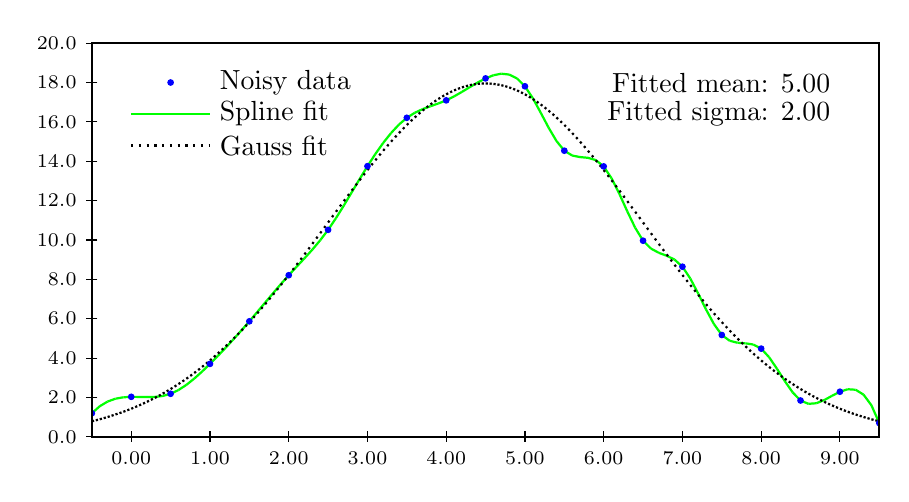
\begin{tikzpicture}
\begin{scope}[]
\clip (0,0) rectangle (10,5);
\begin{scope}[green,thick]
\draw[] (0.0,0.2998554191980206) -- (0.1,0.3886769723521621);
\draw[] (0.1,0.3886769723521621) -- (0.2,0.4483013692841718);
\draw[] (0.2,0.4483013692841718) -- (0.3,0.48433430438467895);
\draw[] (0.3,0.48433430438467895) -- (0.4,0.5023814720443124);
\draw[] (0.4,0.5023814720443124) -- (0.5,0.508048566653701);
\draw[] (0.5,0.508048566653701) -- (0.6,0.506941282603474);
\draw[] (0.6,0.506941282603474) -- (0.7,0.5046653142842601);
\draw[] (0.7,0.5046653142842601) -- (0.8,0.5068263560866882);
\draw[] (0.8,0.5068263560866882) -- (0.9,0.5190301024013876);
\draw[] (0.9,0.5190301024013876) -- (1.0,0.5468822476189868);
\draw[] (1.0,0.5468822476189868) -- (1.1,0.5944637212948228);
\draw[] (1.1,0.5944637212948228) -- (1.2,0.6597563936430622);
\draw[] (1.2,0.6597563936430622) -- (1.3,0.7392173700425795);
\draw[] (1.3,0.7392173700425795) -- (1.4,0.8293037558722491);
\draw[] (1.4,0.8293037558722491) -- (1.5,0.9264726565109458);
\draw[] (1.5,0.9264726565109458) -- (1.6,1.0277622403859983);
\draw[] (1.6,1.0277622403859983) -- (1.7,1.1325349281185535);
\draw[] (1.7,1.1325349281185535) -- (1.8,1.2407342033782138);
\draw[] (1.8,1.2407342033782138) -- (1.9,1.3523035498345806);
\draw[] (1.9,1.3523035498345806) -- (2.0,1.4671864511572559);
\draw[] (2.0,1.4671864511572559) -- (2.1,1.5850318885919035);
\draw[] (2.1,1.5850318885919035) -- (2.2,1.7043108336884367);
\draw[] (2.2,1.7043108336884367) -- (2.3,1.8231997555728292);
\draw[] (2.3,1.8231997555728292) -- (2.4,1.9398751233710578);
\draw[] (2.4,1.9398751233710578) -- (2.5,2.052513406209097);
\draw[] (2.5,2.052513406209097) -- (2.6,2.1603895447518);
\draw[] (2.6,2.1603895447518) -- (2.7,2.2671723658195386);
\draw[] (2.7,2.2671723658195386) -- (2.8,2.37762916777156);
\draw[] (2.8,2.37762916777156) -- (2.9,2.496527248967116);
\draw[] (2.9,2.496527248967116) -- (3.0,2.6286339077654537);
\draw[] (3.0,2.6286339077654537) -- (3.1,2.7769838678261562);
\draw[] (3.1,2.7769838678261562) -- (3.2,2.937681554010137);
\draw[] (3.2,2.937681554010137) -- (3.3,3.1050988164786424);
\draw[] (3.3,3.1050988164786424) -- (3.4,3.2736075053929206);
\draw[] (3.4,3.2736075053929206) -- (3.5,3.437579470914217);
\draw[] (3.5,3.437579470914217) -- (3.6,3.5918608991118726);
\draw[] (3.6,3.5918608991118726) -- (3.7,3.7331953196876033);
\draw[] (3.7,3.7331953196876033) -- (3.8,3.8588005982512175);
\draw[] (3.8,3.8588005982512175) -- (3.9,3.965894600412527);
\draw[] (3.9,3.965894600412527) -- (4.0,4.051695191781341);
\draw[] (4.0,4.051695191781341) -- (4.1,4.115095756069382);
\draw[] (4.1,4.115095756069382) -- (4.2,4.161691749396038);
\draw[] (4.2,4.161691749396038) -- (4.3,4.198754145982606);
\draw[] (4.3,4.198754145982606) -- (4.4,4.233553920050386);
\draw[] (4.4,4.233553920050386) -- (4.5,4.273362045820676);
\draw[] (4.5,4.273362045820676) -- (4.6,4.3234520701688135);
\draw[] (4.6,4.3234520701688135) -- (4.7,4.381107830586282);
\draw[] (4.7,4.381107830586282) -- (4.8,4.441615737218599);
\draw[] (4.8,4.441615737218599) -- (4.9,4.500262200211288);
\draw[] (4.9,4.500262200211288) -- (5.0,4.552333629709862);
\draw[] (5.0,4.552333629709862) -- (5.1,4.59233776594064);
\draw[] (5.1,4.59233776594064) -- (5.2,4.611667669453102);
\draw[] (5.2,4.611667669453102) -- (5.3,4.600937730877521);
\draw[] (5.3,4.600937730877521) -- (5.4,4.550762340844171);
\draw[] (5.4,4.550762340844171) -- (5.5,4.45175588998333);
\draw[] (5.5,4.45175588998333) -- (5.6,4.300437582389341);
\draw[] (5.6,4.300437582389341) -- (5.7,4.116945876012824);
\draw[] (5.7,4.116945876012824) -- (5.8,3.9273240422684816);
\draw[] (5.8,3.9273240422684816) -- (5.9,3.7576153525710008);
\draw[] (5.9,3.7576153525710008) -- (6.0,3.633863078335081);
\draw[] (6.0,3.633863078335081) -- (6.1,3.572659679395789);
\draw[] (6.1,3.572659679395789) -- (6.2,3.5527943692696895);
\draw[] (6.2,3.5527943692696895) -- (6.3,3.543605549893723);
\draw[] (6.3,3.543605549893723) -- (6.4,3.5144316232048283);
\draw[] (6.4,3.5144316232048283) -- (6.5,3.4346109911399463);
\draw[] (6.5,3.4346109911399463) -- (6.6,3.2837879915385906);
\draw[] (6.6,3.2837879915385906) -- (6.7,3.082830705850571);
\draw[] (6.7,3.082830705850571) -- (6.8,2.862913151428279);
\draw[] (6.8,2.862913151428279) -- (6.9,2.655209345624097);
\draw[] (6.9,2.655209345624097) -- (7.0,2.490893305790417);
\draw[] (7.0,2.490893305790417) -- (7.1,2.3911350529230266);
\draw[] (7.1,2.3911350529230266) -- (7.2,2.337088622591336);
\draw[] (7.2,2.337088622591336) -- (7.3,2.299904054008158);
\draw[] (7.3,2.299904054008158) -- (7.4,2.2507313863863057);
\draw[] (7.4,2.2507313863863057) -- (7.5,2.1607206589385934);
\draw[] (7.5,2.1607206589385934) -- (7.6,2.0106625992444567);
\draw[] (7.6,2.0106625992444567) -- (7.7,1.8199106883498228);
\draw[] (7.7,1.8199106883498228) -- (7.8,1.6174590956672459);
\draw[] (7.8,1.6174590956672459) -- (7.9,1.4323019906092747);
\draw[] (7.9,1.4323019906092747) -- (8.0,1.293433542588464);
\draw[] (8.0,1.293433542588464) -- (8.1,1.220344741560056);
\draw[] (8.1,1.220344741560056) -- (8.2,1.1945138596500657);
\draw[] (8.2,1.1945138596500657) -- (8.3,1.1879159895272018);
\draw[] (8.3,1.1879159895272018) -- (8.4,1.172526223860172);
\draw[] (8.4,1.172526223860172) -- (8.5,1.1203196553176844);
\draw[] (8.5,1.1203196553176844) -- (8.6,1.012354246334453);
\draw[] (8.6,1.012354246334453) -- (8.7,0.8660194384092178);
\draw[] (8.7,0.8660194384092178) -- (8.8,0.707787542806721);
\draw[] (8.8,0.707787542806721) -- (8.9,0.5641308707917143);
\draw[] (8.9,0.5641308707917143) -- (9.0,0.46152173362894033);
\draw[] (9.0,0.46152173362894033) -- (9.1,0.41909065427502007);
\draw[] (9.1,0.41909065427502007) -- (9.2,0.4266010024540752);
\draw[] (9.2,0.4266010024540752) -- (9.3,0.46647435958210365);
\draw[] (9.3,0.46647435958210365) -- (9.4,0.5211323070751007);
\draw[] (9.4,0.5211323070751007) -- (9.5,0.5729964263490639);
\draw[] (9.5,0.5729964263490639) -- (9.6,0.6044882988199899);
\draw[] (9.6,0.6044882988199899) -- (9.7,0.5980295059038759);
\draw[] (9.7,0.5980295059038759) -- (9.8,0.5360416290167176);
\draw[] (9.8,0.5360416290167176) -- (9.9,0.4009462495745133);
\draw[] (9.9,0.4009462495745133) -- (10.0,0.1751649489932598);
\end{scope}
\begin{scope}[dotted, thick]
\draw[] (0.0,0.19719338055255084) -- (0.05,0.20984567391293701);
\draw[] (0.05,0.20984567391293701) -- (0.1,0.2231702369075935);
\draw[] (0.1,0.2231702369075935) -- (0.15,0.23719257748861314);
\draw[] (0.15,0.23719257748861314) -- (0.2,0.25193846581686985);
\draw[] (0.2,0.25193846581686985) -- (0.25,0.26743388433641285);
\draw[] (0.25,0.26743388433641285) -- (0.3,0.2837049740458145);
\draw[] (0.3,0.2837049740458145) -- (0.35,0.3007779769376655);
\draw[] (0.35,0.3007779769376655) -- (0.4,0.3186791745928813);
\draw[] (0.4,0.3186791745928813) -- (0.45,0.33743482293299765);
\draw[] (0.45,0.33743482293299765) -- (0.5,0.3570710831511164);
\draw[] (0.5,0.3570710831511164) -- (0.55,0.37761394886060007);
\draw[] (0.55,0.37761394886060007) -- (0.6,0.3990891695199511);
\draw[] (0.6,0.3990891695199511) -- (0.65,0.42152217021247246);
\draw[] (0.65,0.42152217021247246) -- (0.7,0.444937967880252);
\draw[] (0.7,0.444937967880252) -- (0.75,0.46936108413364097);
\draw[] (0.75,0.46936108413364097) -- (0.8,0.49481545477963207);
\draw[] (0.8,0.49481545477963207) -- (0.85,0.5213243362352994);
\draw[] (0.85,0.5213243362352994) -- (0.9,0.5489102090156216);
\draw[] (0.9,0.5489102090156216) -- (0.95,0.5775946785084662);
\draw[] (0.95,0.5775946785084662) -- (1.0,0.60739837327317);
\draw[] (1.0,0.60739837327317) -- (1.05,0.6383408411228194);
\draw[] (1.05,0.6383408411228194) -- (1.1,0.6704404432739747);
\draw[] (1.1,0.6704404432739747) -- (1.15,0.7037142468709632);
\draw[] (1.15,0.7037142468709632) -- (1.2,0.738177916214895);
\draw[] (1.2,0.738177916214895) -- (1.25,0.7738456030500619);
\draw[] (1.25,0.7738456030500619) -- (1.3,0.8107298362822254);
\draw[] (1.3,0.8107298362822254) -- (1.35,0.8488414115242828);
\draw[] (1.35,0.8488414115242828) -- (1.4,0.8881892808848224);
\draw[] (1.4,0.8881892808848224) -- (1.45,0.9287804434339139);
\draw[] (1.45,0.9287804434339139) -- (1.5,0.9706198367980078);
\draw[] (1.5,0.9706198367980078) -- (1.55,1.0137102303518524);
\draw[] (1.55,1.0137102303518524) -- (1.6,1.0580521204897222);
\draw[] (1.6,1.0580521204897222) -- (1.65,1.1036436284708402);
\draw[] (1.65,1.1036436284708402) -- (1.7,1.1504804013444883);
\draw[] (1.7,1.1504804013444883) -- (1.75,1.1985555164688135);
\draw[] (1.75,1.1985555164688135) -- (1.8,1.2478593901436028);
\draw[] (1.8,1.2478593901436028) -- (1.85,1.2983796908811616);
\draw[] (1.85,1.2983796908811616) -- (1.9,1.350101257840809);
\draw[] (1.9,1.350101257840809) -- (1.95,1.4030060249512366);
\draw[] (1.95,1.4030060249512366) -- (2.0,1.4570729512409966);
\draw[] (2.0,1.4570729512409966) -- (2.05,1.5122779578906014);
\draw[] (2.05,1.5122779578906014) -- (2.1,1.5685938725100126);
\draw[] (2.1,1.5685938725100126) -- (2.15,1.6259903811327017);
\draw[] (2.15,1.6259903811327017) -- (2.2,1.6844339884018351);
\draw[] (2.2,1.6844339884018351) -- (2.25,1.743887986405502);
\draw[] (2.25,1.743887986405502) -- (2.3,1.8043124325962971);
\draw[] (2.3,1.8043124325962971) -- (2.35,1.865664137205879);
\draw[] (2.35,1.865664137205879) -- (2.4,1.9278966605375325);
\draw[] (2.4,1.9278966605375325) -- (2.45,1.9909603204892214);
\draw[] (2.45,1.9909603204892214) -- (2.5,2.0548022106261956);
\draw[] (2.5,2.0548022106261956) -- (2.55,2.11936622908612);
\draw[] (2.55,2.11936622908612) -- (2.6,2.184593118560845);
\draw[] (2.6,2.184593118560845) -- (2.65,2.250420517557687);
\draw[] (2.65,2.250420517557687) -- (2.7,2.3167830230994166);
\draw[] (2.7,2.3167830230994166) -- (2.75,2.3836122649763207);
\draw[] (2.75,2.3836122649763207) -- (2.8,2.4508369916158963);
\draw[] (2.8,2.4508369916158963) -- (2.85,2.5183831675861494);
\draw[] (2.85,2.5183831675861494) -- (2.9,2.586174082697328);
\draw[] (2.9,2.586174082697328) -- (2.95,2.654130472614525);
\draw[] (2.95,2.654130472614525) -- (3.0,2.722170650840074);
\draw[] (3.0,2.722170650840074) -- (3.05,2.7902106518705065);
\draw[] (3.05,2.7902106518705065) -- (3.1,2.8581643852780934);
\draw[] (3.1,2.8581643852780934) -- (3.15,2.925943800412172);
\draw[] (3.15,2.925943800412172) -- (3.2,2.9934590613607153);
\draw[] (3.2,2.9934590613607153) -- (3.25,3.0606187317583413);
\draw[] (3.25,3.0606187317583413) -- (3.3,3.127329968973441);
\draw[] (3.3,3.127329968973441) -- (3.35,3.193498727154717);
\draw[] (3.35,3.193498727154717) -- (3.4,3.2590299685664195);
\draw[] (3.4,3.2590299685664195) -- (3.45,3.323827882592326);
\draw[] (3.45,3.323827882592326) -- (3.5,3.387796111741297);
\draw[] (3.5,3.387796111741297) -- (3.55,3.450837983942451);
\draw[] (3.55,3.450837983942451) -- (3.6,3.5128567503758203);
\draw[] (3.6,3.5128567503758203) -- (3.65,3.5737558280451784);
\draw[] (3.65,3.5737558280451784) -- (3.7,3.6334390462638013);
\draw[] (3.7,3.6334390462638013) -- (3.75,3.6918108961914897);
\draw[] (3.75,3.6918108961914897) -- (3.8,3.7487767825325204);
\draw[] (3.8,3.7487767825325204) -- (3.85,3.804243276479533);
\draw[] (3.85,3.804243276479533) -- (3.9,3.858118368967853);
\draw[] (3.9,3.858118368967853) -- (3.95,3.910311723288705);
\draw[] (3.95,3.910311723288705) -- (4.0,3.9607349260981626);
\draw[] (4.0,3.9607349260981626) -- (4.05,4.009301735851859);
\draw[] (4.05,4.009301735851859) -- (4.1,4.0559283276933416);
\draw[] (4.1,4.0559283276933416) -- (4.15,4.100533533826755);
\draw[] (4.15,4.100533533826755) -- (4.2,4.143039078412198);
\draw[] (4.2,4.143039078412198) -- (4.25,4.183369806034715);
\draw[] (4.25,4.183369806034715) -- (4.3,4.2214539028153695);
\draw[] (4.3,4.2214539028153695) -- (4.35,4.257223109255291);
\draw[] (4.35,4.257223109255291) -- (4.4,4.290612923930722);
\draw[] (4.4,4.290612923930722) -- (4.45,4.321562797189007);
\draw[] (4.45,4.321562797189007) -- (4.5,4.350016314031885);
\draw[] (4.5,4.350016314031885) -- (4.55,4.375921365413266);
\draw[] (4.55,4.375921365413266) -- (4.6,4.399230307223716);
\draw[] (4.6,4.399230307223716) -- (4.65,4.4199001062828565);
\draw[] (4.65,4.4199001062828565) -- (4.7,4.4378924727135916);
\draw[] (4.7,4.4378924727135916) -- (4.75,4.453173978128275);
\draw[] (4.75,4.453173978128275) -- (4.8,4.465716159116226);
\draw[] (4.8,4.465716159116226) -- (4.85,4.475495605584188);
\draw[] (4.85,4.475495605584188) -- (4.9,4.482494033565941);
\draw[] (4.9,4.482494033565941) -- (4.95,4.486698342184142);
\draw[] (4.95,4.486698342184142) -- (5.0,4.488100654515964);
\draw[] (5.0,4.488100654515964) -- (5.05,4.486698342184142);
\draw[] (5.05,4.486698342184142) -- (5.1,4.482494033565941);
\draw[] (5.1,4.482494033565941) -- (5.15,4.475495605584188);
\draw[] (5.15,4.475495605584188) -- (5.2,4.465716159116226);
\draw[] (5.2,4.465716159116226) -- (5.25,4.453173978128275);
\draw[] (5.25,4.453173978128275) -- (5.3,4.4378924727135916);
\draw[] (5.3,4.4378924727135916) -- (5.35,4.4199001062828565);
\draw[] (5.35,4.4199001062828565) -- (5.4,4.399230307223716);
\draw[] (5.4,4.399230307223716) -- (5.45,4.375921365413266);
\draw[] (5.45,4.375921365413266) -- (5.5,4.350016314031885);
\draw[] (5.5,4.350016314031885) -- (5.55,4.321562797189007);
\draw[] (5.55,4.321562797189007) -- (5.6,4.290612923930722);
\draw[] (5.6,4.290612923930722) -- (5.65,4.257223109255291);
\draw[] (5.65,4.257223109255291) -- (5.7,4.2214539028153695);
\draw[] (5.7,4.2214539028153695) -- (5.75,4.183369806034715);
\draw[] (5.75,4.183369806034715) -- (5.8,4.143039078412198);
\draw[] (5.8,4.143039078412198) -- (5.85,4.100533533826755);
\draw[] (5.85,4.100533533826755) -- (5.9,4.0559283276933416);
\draw[] (5.9,4.0559283276933416) -- (5.95,4.009301735851859);
\draw[] (5.95,4.009301735851859) -- (6.0,3.9607349260981626);
\draw[] (6.0,3.9607349260981626) -- (6.05,3.910311723288705);
\draw[] (6.05,3.910311723288705) -- (6.1,3.8581183689678533);
\draw[] (6.1,3.8581183689678533) -- (6.15,3.8042432764795326);
\draw[] (6.15,3.8042432764795326) -- (6.2,3.7487767825325204);
\draw[] (6.2,3.7487767825325204) -- (6.25,3.6918108961914897);
\draw[] (6.25,3.6918108961914897) -- (6.3,3.6334390462638013);
\draw[] (6.3,3.6334390462638013) -- (6.35,3.573755828045179);
\draw[] (6.35,3.573755828045179) -- (6.4,3.51285675037582);
\draw[] (6.4,3.51285675037582) -- (6.45,3.450837983942451);
\draw[] (6.45,3.450837983942451) -- (6.5,3.387796111741297);
\draw[] (6.5,3.387796111741297) -- (6.55,3.323827882592326);
\draw[] (6.55,3.323827882592326) -- (6.6,3.25902996856642);
\draw[] (6.6,3.25902996856642) -- (6.65,3.1934987271547164);
\draw[] (6.65,3.1934987271547164) -- (6.7,3.127329968973441);
\draw[] (6.7,3.127329968973441) -- (6.75,3.0606187317583413);
\draw[] (6.75,3.0606187317583413) -- (6.8,2.9934590613607153);
\draw[] (6.8,2.9934590613607153) -- (6.85,2.9259438004121723);
\draw[] (6.85,2.9259438004121723) -- (6.9,2.8581643852780925);
\draw[] (6.9,2.8581643852780925) -- (6.95,2.7902106518705065);
\draw[] (6.95,2.7902106518705065) -- (7.0,2.722170650840074);
\draw[] (7.0,2.722170650840074) -- (7.05,2.654130472614525);
\draw[] (7.05,2.654130472614525) -- (7.1,2.5861740826973287);
\draw[] (7.1,2.5861740826973287) -- (7.15,2.5183831675861486);
\draw[] (7.15,2.5183831675861486) -- (7.2,2.4508369916158963);
\draw[] (7.2,2.4508369916158963) -- (7.25,2.3836122649763207);
\draw[] (7.25,2.3836122649763207) -- (7.3,2.3167830230994166);
\draw[] (7.3,2.3167830230994166) -- (7.35,2.2504205175576875);
\draw[] (7.35,2.2504205175576875) -- (7.4,2.1845931185608447);
\draw[] (7.4,2.1845931185608447) -- (7.45,2.11936622908612);
\draw[] (7.45,2.11936622908612) -- (7.5,2.0548022106261956);
\draw[] (7.5,2.0548022106261956) -- (7.55,1.9909603204892214);
\draw[] (7.55,1.9909603204892214) -- (7.6,1.927896660537533);
\draw[] (7.6,1.927896660537533) -- (7.65,1.8656641372058782);
\draw[] (7.65,1.8656641372058782) -- (7.7,1.8043124325962971);
\draw[] (7.7,1.8043124325962971) -- (7.75,1.743887986405502);
\draw[] (7.75,1.743887986405502) -- (7.8,1.6844339884018351);
\draw[] (7.8,1.6844339884018351) -- (7.85,1.6259903811327023);
\draw[] (7.85,1.6259903811327023) -- (7.9,1.5685938725100121);
\draw[] (7.9,1.5685938725100121) -- (7.95,1.5122779578906014);
\draw[] (7.95,1.5122779578906014) -- (8.0,1.4570729512409966);
\draw[] (8.0,1.4570729512409966) -- (8.05,1.4030060249512355);
\draw[] (8.05,1.4030060249512355) -- (8.1,1.3501012578408094);
\draw[] (8.1,1.3501012578408094) -- (8.15,1.298379690881161);
\draw[] (8.15,1.298379690881161) -- (8.2,1.2478593901436035);
\draw[] (8.2,1.2478593901436035) -- (8.25,1.1985555164688135);
\draw[] (8.25,1.1985555164688135) -- (8.3,1.1504804013444876);
\draw[] (8.3,1.1504804013444876) -- (8.35,1.1036436284708406);
\draw[] (8.35,1.1036436284708406) -- (8.4,1.0580521204897217);
\draw[] (8.4,1.0580521204897217) -- (8.45,1.013710230351853);
\draw[] (8.45,1.013710230351853) -- (8.5,0.9706198367980078);
\draw[] (8.5,0.9706198367980078) -- (8.55,0.9287804434339132);
\draw[] (8.55,0.9287804434339132) -- (8.6,0.8881892808848225);
\draw[] (8.6,0.8881892808848225) -- (8.65,0.8488414115242826);
\draw[] (8.65,0.8488414115242826) -- (8.7,0.8107298362822261);
\draw[] (8.7,0.8107298362822261) -- (8.75,0.7738456030500619);
\draw[] (8.75,0.7738456030500619) -- (8.8,0.7381779162148944);
\draw[] (8.8,0.7381779162148944) -- (8.85,0.7037142468709636);
\draw[] (8.85,0.7037142468709636) -- (8.9,0.6704404432739745);
\draw[] (8.9,0.6704404432739745) -- (8.95,0.63834084112282);
\draw[] (8.95,0.63834084112282) -- (9.0,0.60739837327317);
\draw[] (9.0,0.60739837327317) -- (9.05,0.5775946785084658);
\draw[] (9.05,0.5775946785084658) -- (9.1,0.5489102090156216);
\draw[] (9.1,0.5489102090156216) -- (9.15,0.5213243362352994);
\draw[] (9.15,0.5213243362352994) -- (9.2,0.4948154547796325);
\draw[] (9.2,0.4948154547796325) -- (9.25,0.46936108413364097);
\draw[] (9.25,0.46936108413364097) -- (9.3,0.4449379678802516);
\draw[] (9.3,0.4449379678802516) -- (9.35,0.42152217021247246);
\draw[] (9.35,0.42152217021247246) -- (9.4,0.3990891695199511);
\draw[] (9.4,0.3990891695199511) -- (9.45,0.37761394886060046);
\draw[] (9.45,0.37761394886060046) -- (9.5,0.3570710831511164);
\draw[] (9.5,0.3570710831511164) -- (9.55,0.3374348229329973);
\draw[] (9.55,0.3374348229329973) -- (9.6,0.3186791745928813);
\draw[] (9.6,0.3186791745928813) -- (9.65,0.3007779769376655);
\draw[] (9.65,0.3007779769376655) -- (9.7,0.2837049740458149);
\draw[] (9.7,0.2837049740458149) -- (9.75,0.26743388433641285);
\draw[] (9.75,0.26743388433641285) -- (9.8,0.25193846581686963);
\draw[] (9.8,0.25193846581686963) -- (9.85,0.23719257748861314);
\draw[] (9.85,0.23719257748861314) -- (9.9,0.2231702369075935);
\draw[] (9.9,0.2231702369075935) -- (9.95,0.2098456739129372);
\draw[] (9.95,0.2098456739129372) -- (10.0,0.19719338055255084);
\end{scope}
\draw[draw=blue,fill=blue] (0.0,0.2998554191980206) circle(1pt); 
\draw[draw=blue,fill=blue] (0.5,0.5080485666537011) circle(1pt); 
\draw[draw=blue,fill=blue] (1.0,0.5468822476189868) circle(1pt); 
\draw[draw=blue,fill=blue] (1.5,0.9264726565109457) circle(1pt); 
\draw[draw=blue,fill=blue] (2.0,1.4671864511572559) circle(1pt); 
\draw[draw=blue,fill=blue] (2.5,2.052513406209097) circle(1pt); 
\draw[draw=blue,fill=blue] (3.0,2.6286339077654537) circle(1pt); 
\draw[draw=blue,fill=blue] (3.5,3.437579470914217) circle(1pt); 
\draw[draw=blue,fill=blue] (4.0,4.051695191781341) circle(1pt); 
\draw[draw=blue,fill=blue] (4.5,4.273362045820676) circle(1pt); 
\draw[draw=blue,fill=blue] (5.0,4.552333629709863) circle(1pt); 
\draw[draw=blue,fill=blue] (5.5,4.45175588998333) circle(1pt); 
\draw[draw=blue,fill=blue] (6.0,3.633863078335081) circle(1pt); 
\draw[draw=blue,fill=blue] (6.5,3.4346109911399463) circle(1pt); 
\draw[draw=blue,fill=blue] (7.0,2.490893305790417) circle(1pt); 
\draw[draw=blue,fill=blue] (7.5,2.1607206589385934) circle(1pt); 
\draw[draw=blue,fill=blue] (8.0,1.293433542588464) circle(1pt); 
\draw[draw=blue,fill=blue] (8.5,1.1203196553176844) circle(1pt); 
\draw[draw=blue,fill=blue] (9.0,0.46152173362894033) circle(1pt); 
\draw[draw=blue,fill=blue] (9.5,0.5729964263490638) circle(1pt); 
\draw[draw=blue,fill=blue] (10.0,0.17516494899325974) circle(1pt); 
\end{scope}
\draw (0.5,0cm + 2pt) -- (0.5, 0cm -2pt) node[below] {\scriptsize{\num[round-mode=places,round-precision=2]{0}}};
\draw (1.5,0cm + 2pt) -- (1.5, 0cm -2pt) node[below] {\scriptsize{\num[round-mode=places,round-precision=2]{1}}};
\draw (2.5,0cm + 2pt) -- (2.5, 0cm -2pt) node[below] {\scriptsize{\num[round-mode=places,round-precision=2]{2}}};
\draw (3.5,0cm + 2pt) -- (3.5, 0cm -2pt) node[below] {\scriptsize{\num[round-mode=places,round-precision=2]{3}}};
\draw (4.5,0cm + 2pt) -- (4.5, 0cm -2pt) node[below] {\scriptsize{\num[round-mode=places,round-precision=2]{4}}};
\draw (5.5,0cm + 2pt) -- (5.5, 0cm -2pt) node[below] {\scriptsize{\num[round-mode=places,round-precision=2]{5}}};
\draw (6.5,0cm + 2pt) -- (6.5, 0cm -2pt) node[below] {\scriptsize{\num[round-mode=places,round-precision=2]{6}}};
\draw (7.5,0cm + 2pt) -- (7.5, 0cm -2pt) node[below] {\scriptsize{\num[round-mode=places,round-precision=2]{7}}};
\draw (8.5,0cm + 2pt) -- (8.5, 0cm -2pt) node[below] {\scriptsize{\num[round-mode=places,round-precision=2]{8}}};
\draw (9.5,0cm + 2pt) -- (9.5, 0cm -2pt) node[below] {\scriptsize{\num[round-mode=places,round-precision=2]{9}}};
\draw (0cm + 2pt,0.    ) -- (0cm-2pt,0.    ) node[left] {\scriptsize{\num[round-mode=places,round-precision=1]{0}}};
\draw (0cm + 2pt,0.5    ) -- (0cm-2pt,0.5    ) node[left] {\scriptsize{\num[round-mode=places,round-precision=1]{2}}};
\draw (0cm + 2pt,1.    ) -- (0cm-2pt,1.    ) node[left] {\scriptsize{\num[round-mode=places,round-precision=1]{4}}};
\draw (0cm + 2pt,1.5    ) -- (0cm-2pt,1.5    ) node[left] {\scriptsize{\num[round-mode=places,round-precision=1]{6}}};
\draw (0cm + 2pt,2.    ) -- (0cm-2pt,2.    ) node[left] {\scriptsize{\num[round-mode=places,round-precision=1]{8}}};
\draw (0cm + 2pt,2.5    ) -- (0cm-2pt,2.5    ) node[left] {\scriptsize{\num[round-mode=places,round-precision=1]{10}}};
\draw (0cm + 2pt,3.    ) -- (0cm-2pt,3.    ) node[left] {\scriptsize{\num[round-mode=places,round-precision=1]{12}}};
\draw (0cm + 2pt,3.5    ) -- (0cm-2pt,3.5    ) node[left] {\scriptsize{\num[round-mode=places,round-precision=1]{14}}};
\draw (0cm + 2pt,4.    ) -- (0cm-2pt,4.    ) node[left] {\scriptsize{\num[round-mode=places,round-precision=1]{16}}};
\draw (0cm + 2pt,4.5    ) -- (0cm-2pt,4.5    ) node[left] {\scriptsize{\num[round-mode=places,round-precision=1]{18}}};
\draw (0cm + 2pt,5.    ) -- (0cm-2pt,5.    ) node[left] {\scriptsize{\num[round-mode=places,round-precision=1]{20}}};
\draw[draw=blue,fill=blue] (1.0,4.5) circle(1pt); 
\node[right,] at (1.5,4.5) {Noisy data};
\draw[draw=green,thick] (0.5,4.1) -- (1.5,4.1);
\node[right,] at (1.5,4.1) {Spline fit};
\draw[thick,dotted] (0.5,3.7) -- (1.5,3.7);
\node[right,] at (1.5,3.7) {Gauss fit};
\node[left] at (9.5,4.5) {Fitted mean:  5.00};
\node[left] at (9.5,4.1) {Fitted sigma:  2.00};
\draw[thick] (0,0) rectangle (10,5);
\end{tikzpicture}
%%% Local Variables: 
%%% mode: latex 
%%% TeX-master: "master" 
%%% End:


\captionsetup{singlelinecheck=off}
\caption[asdf]{Some Gauss smeared data points, fitted with the Gaussian function. Fit parameters are printed in the plot. 
A spline fit is also plotted.}
\end{figure}
\begin{figure}[H]
\centering
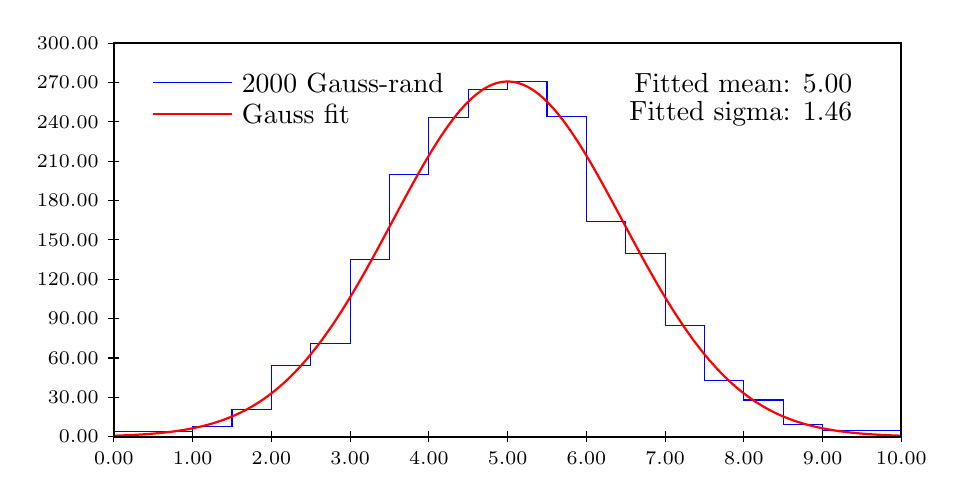
\begin{tikzpicture}[]
\begin{scope}[]
\clip (0.0,0.0) rectangle (10.0,5.0);
\begin{scope}[shift={(0.0,0.0)}]
\pgfsetxvec{\pgfpoint{1.0cm}{0cm}}
\pgfsetyvec{\pgfpoint{0cm}{0.016666668cm}}
\begin{scope}[shift={(0.0,0.0)}]
\begin{scope}[draw=blue]
\pgfpathmoveto{ \pgfpointxy {10.0} {0.0}}
\pgfpathlineto{ \pgfpointxy {10.0} {5.0}}
\pgfpathlineto{ \pgfpointxy {9.5} {5.0}}
\pgfpathlineto{ \pgfpointxy {9.5} {5.0}}
\pgfpathlineto{ \pgfpointxy {9.0} {5.0}}
\pgfpathlineto{ \pgfpointxy {9.0} {9.0}}
\pgfpathlineto{ \pgfpointxy {8.5} {9.0}}
\pgfpathlineto{ \pgfpointxy {8.5} {28.0}}
\pgfpathlineto{ \pgfpointxy {8.0} {28.0}}
\pgfpathlineto{ \pgfpointxy {8.0} {43.0}}
\pgfpathlineto{ \pgfpointxy {7.5} {43.0}}
\pgfpathlineto{ \pgfpointxy {7.5} {85.0}}
\pgfpathlineto{ \pgfpointxy {7.0} {85.0}}
\pgfpathlineto{ \pgfpointxy {7.0} {140.0}}
\pgfpathlineto{ \pgfpointxy {6.5} {140.0}}
\pgfpathlineto{ \pgfpointxy {6.5} {164.0}}
\pgfpathlineto{ \pgfpointxy {6.0} {164.0}}
\pgfpathlineto{ \pgfpointxy {6.0} {244.0}}
\pgfpathlineto{ \pgfpointxy {5.5} {244.0}}
\pgfpathlineto{ \pgfpointxy {5.5} {271.0}}
\pgfpathlineto{ \pgfpointxy {5.0} {271.0}}
\pgfpathlineto{ \pgfpointxy {5.0} {265.0}}
\pgfpathlineto{ \pgfpointxy {4.5} {265.0}}
\pgfpathlineto{ \pgfpointxy {4.5} {243.0}}
\pgfpathlineto{ \pgfpointxy {4.0} {243.0}}
\pgfpathlineto{ \pgfpointxy {4.0} {200.0}}
\pgfpathlineto{ \pgfpointxy {3.5} {200.0}}
\pgfpathlineto{ \pgfpointxy {3.5} {135.0}}
\pgfpathlineto{ \pgfpointxy {3.0} {135.0}}
\pgfpathlineto{ \pgfpointxy {3.0} {71.0}}
\pgfpathlineto{ \pgfpointxy {2.5} {71.0}}
\pgfpathlineto{ \pgfpointxy {2.5} {54.0}}
\pgfpathlineto{ \pgfpointxy {2.0} {54.0}}
\pgfpathlineto{ \pgfpointxy {2.0} {21.0}}
\pgfpathlineto{ \pgfpointxy {1.5} {21.0}}
\pgfpathlineto{ \pgfpointxy {1.5} {8.0}}
\pgfpathlineto{ \pgfpointxy {1.0} {8.0}}
\pgfpathlineto{ \pgfpointxy {1.0} {4.0}}
\pgfpathlineto{ \pgfpointxy {0.5} {4.0}}
\pgfpathlineto{ \pgfpointxy {0.5} {4.0}}
\pgfpathlineto{ \pgfpointxy {0.0} {4.0}}
\pgfpathlineto{ \pgfpointxy {0.0} {0.0}}
\pgfusepath{ stroke, }
\end{scope}
\end{scope}
\pgfsetxvec{\pgfpoint{1cm}{0cm}}
\pgfsetyvec{\pgfpoint{0cm}{1cm}}
\end{scope}
\end{scope}
\node[left] at (9.5,4.5) {Fitted mean:  5.00};
\node[left] at (9.5,4.1) {Fitted sigma:  1.46};
\begin{scope}[]
\clip (0.0,0.0) rectangle (10.0,5.0);
\begin{scope}[shift={(0.0,0.0)}]
\pgfsetxvec{\pgfpoint{1.0cm}{0cm}}
\pgfsetyvec{\pgfpoint{0cm}{0.016666668cm}}
\begin{scope}[shift={(0.0,0.0)}]
\begin{scope}[thick,red]
\pgfpathmoveto{ \pgfpointxy {0.0} {0.785533585190544}}
\pgfpathlineto{ \pgfpointxy {0.05} {0.8823944062104124}}
\pgfpathlineto{ \pgfpointxy {0.1} {0.9900410132316494}}
\pgfpathlineto{ \pgfpointxy {0.15} {1.1095224058046345}}
\pgfpathlineto{ \pgfpointxy {0.2} {1.2419708963422873}}
\pgfpathlineto{ \pgfpointxy {0.25} {1.3886065589283518}}
\pgfpathlineto{ \pgfpointxy {0.3} {1.5507416694118887}}
\pgfpathlineto{ \pgfpointxy {0.35} {1.7297851028337528}}
\pgfpathlineto{ \pgfpointxy {0.4} {1.927246650571349}}
\pgfpathlineto{ \pgfpointxy {0.45} {2.144741215868452}}
\pgfpathlineto{ \pgfpointxy {0.5} {2.383992842671168}}
\pgfpathlineto{ \pgfpointxy {0.55} {2.646838528957892}}
\pgfpathlineto{ \pgfpointxy {0.6} {2.935231772073318}}
\pgfpathlineto{ \pgfpointxy {0.65} {3.251245790000996}}
\pgfpathlineto{ \pgfpointxy {0.7} {3.5970763590868597}}
\pgfpathlineto{ \pgfpointxy {0.75} {3.9750442055123947}}
\pgfpathlineto{ \pgfpointxy {0.8} {4.387596884868998}}
\pgfpathlineto{ \pgfpointxy {0.85} {4.8373100815661525}}
\pgfpathlineto{ \pgfpointxy {0.9} {5.326888257579253}}
\pgfpathlineto{ \pgfpointxy {0.95} {5.859164578274084}}
\pgfpathlineto{ \pgfpointxy {1.0} {6.437100041802212}}
\pgfpathlineto{ \pgfpointxy {1.05} {7.063781737911131}}
\pgfpathlineto{ \pgfpointxy {1.1} {7.742420162024598}}
\pgfpathlineto{ \pgfpointxy {1.15} {8.476345511186555}}
\pgfpathlineto{ \pgfpointxy {1.2} {9.269002889991516}}
\pgfpathlineto{ \pgfpointxy {1.25} {10.12394635700542}}
\pgfpathlineto{ \pgfpointxy {1.3} {11.044831745470251}}
\pgfpathlineto{ \pgfpointxy {1.35} {12.035408196332893}}
\pgfpathlineto{ \pgfpointxy {1.4} {13.099508346888094}}
\pgfpathlineto{ \pgfpointxy {1.45} {14.241037124611898}}
\pgfpathlineto{ \pgfpointxy {1.5} {15.463959103111062}}
\pgfpathlineto{ \pgfpointxy {1.55} {16.77228438554224}}
\pgfpathlineto{ \pgfpointxy {1.6} {18.170052990364315}}
\pgfpathlineto{ \pgfpointxy {1.65} {19.661317724870088}}
\pgfpathlineto{ \pgfpointxy {1.7} {21.250125543575855}}
\pgfpathlineto{ \pgfpointxy {1.75} {22.940497401191028}}
\pgfpathlineto{ \pgfpointxy {1.8} {24.736406623493174}}
\pgfpathlineto{ \pgfpointxy {1.85} {26.64175583392414}}
\pgfpathlineto{ \pgfpointxy {1.9} {28.660352489018294}}
\pgfpathlineto{ \pgfpointxy {1.95} {30.795883091768726}}
\pgfpathlineto{ \pgfpointxy {2.0} {33.05188616861204}}
\pgfpathlineto{ \pgfpointxy {2.05} {35.431724112736475}}
\pgfpathlineto{ \pgfpointxy {2.1} {37.938554013731526}}
\pgfpathlineto{ \pgfpointxy {2.15} {40.57529761104231}}
\pgfpathlineto{ \pgfpointxy {2.2} {43.34461052608296}}
\pgfpathlineto{ \pgfpointxy {2.25} {46.248850945007725}}
\pgfpathlineto{ \pgfpointxy {2.3} {49.290047940835414}}
\pgfpathlineto{ \pgfpointxy {2.35} {52.46986963965609}}
\pgfpathlineto{ \pgfpointxy {2.4} {55.789591450800295}}
\pgfpathlineto{ \pgfpointxy {2.45} {59.25006459489787}}
\pgfpathlineto{ \pgfpointxy {2.5} {62.85168517646614}}
\pgfpathlineto{ \pgfpointxy {2.55} {66.5943640588275}}
\pgfpathlineto{ \pgfpointxy {2.6} {70.47749780853638}}
\pgfpathlineto{ \pgfpointxy {2.65} {74.49994098389061}}
\pgfpathlineto{ \pgfpointxy {2.7} {78.65998004730363}}
\pgfpathlineto{ \pgfpointxy {2.75} {82.9553091841374}}
\pgfpathlineto{ \pgfpointxy {2.8} {87.38300831087108}}
\pgfpathlineto{ \pgfpointxy {2.85} {91.93952355305386}}
\pgfpathlineto{ \pgfpointxy {2.9} {96.62065046824108}}
\pgfpathlineto{ \pgfpointxy {2.95} {101.42152028093761}}
\pgfpathlineto{ \pgfpointxy {3.0} {106.33658938540171}}
\pgfpathlineto{ \pgfpointxy {3.05} {111.35963235796345}}
\pgfpathlineto{ \pgfpointxy {3.1} {116.48373870327391}}
\pgfpathlineto{ \pgfpointxy {3.15} {121.70131353866445}}
\pgfpathlineto{ \pgfpointxy {3.2} {127.00408239762504}}
\pgfpathlineto{ \pgfpointxy {3.25} {132.38310030741803}}
\pgfpathlineto{ \pgfpointxy {3.3} {137.82876526717794}}
\pgfpathlineto{ \pgfpointxy {3.35} {143.3308362216892}}
\pgfpathlineto{ \pgfpointxy {3.4} {148.87845559261598}}
\pgfpathlineto{ \pgfpointxy {3.45} {154.4601763935346}}
\pgfpathlineto{ \pgfpointxy {3.5} {160.06399391798755}}
\pgfpathlineto{ \pgfpointxy {3.55} {165.67738195127163}}
\pgfpathlineto{ \pgfpointxy {3.6} {171.28733341714147}}
\pgfpathlineto{ \pgfpointxy {3.65} {176.88040533044696}}
\pgfpathlineto{ \pgfpointxy {3.7} {182.4427678863249}}
\pgfpathlineto{ \pgfpointxy {3.75} {187.96025747636367}}
\pgfpathlineto{ \pgfpointxy {3.8} {193.4184333825861}}
\pgfpathlineto{ \pgfpointxy {3.85} {198.8026378615926}}
\pgfpathlineto{ \pgfpointxy {3.9} {204.0980592942233}}
\pgfpathlineto{ \pgfpointxy {3.95} {209.2897980410712}}
\pgfpathlineto{ \pgfpointxy {4.0} {214.36293461154008}}
\pgfpathlineto{ \pgfpointxy {4.05} {219.30259972431023}}
\pgfpathlineto{ \pgfpointxy {4.1} {224.09404581043842}}
\pgfpathlineto{ \pgfpointxy {4.15} {228.7227194872519}}
\pgfpathlineto{ \pgfpointxy {4.2} {233.1743345120225}}
\pgfpathlineto{ \pgfpointxy {4.25} {237.43494470943358}}
\pgfpathlineto{ \pgfpointxy {4.3} {241.4910163563196}}
\pgfpathlineto{ \pgfpointxy {4.35} {245.32949950128543}}
\pgfpathlineto{ \pgfpointxy {4.4} {248.93789769574337}}
\pgfpathlineto{ \pgfpointxy {4.45} {252.30433561675085}}
\pgfpathlineto{ \pgfpointxy {4.5} {255.4176240708332}}
\pgfpathlineto{ \pgfpointxy {4.55} {258.26732188172053}}
\pgfpathlineto{ \pgfpointxy {4.6} {260.84379418355206}}
\pgfpathlineto{ \pgfpointxy {4.65} {263.13826666446903}}
\pgfpathlineto{ \pgfpointxy {4.7} {265.14287533345066}}
\pgfpathlineto{ \pgfpointxy {4.75} {266.8507114154981}}
\pgfpathlineto{ \pgfpointxy {4.8} {268.25586101655}}
\pgfpathlineto{ \pgfpointxy {4.85} {269.35343923947187}}
\pgfpathlineto{ \pgfpointxy {4.9} {270.1396184757107}}
\pgfpathlineto{ \pgfpointxy {4.95} {270.6116506433102}}
\pgfpathlineto{ \pgfpointxy {5.0} {270.76788319047864}}
\pgfpathlineto{ \pgfpointxy {5.05} {270.6077687342832}}
\pgfpathlineto{ \pgfpointxy {5.1} {270.1318682557956}}
\pgfpathlineto{ \pgfpointxy {5.15} {269.3418478255878}}
\pgfpathlineto{ \pgfpointxy {5.2} {268.24046888632785}}
\pgfpathlineto{ \pgfpointxy {5.25} {266.8315721717906}}
\pgfpathlineto{ \pgfpointxy {5.3} {265.1200553933392}}
\pgfpathlineto{ \pgfpointxy {5.35} {263.11184487529204}}
\pgfpathlineto{ \pgfpointxy {5.4} {260.81386136906104}}
\pgfpathlineto{ \pgfpointxy {5.45} {258.23398032201965}}
\pgfpathlineto{ \pgfpointxy {5.5} {255.38098692026887}}
\pgfpathlineto{ \pgfpointxy {5.55} {252.26452626438723}}
\pgfpathlineto{ \pgfpointxy {5.6} {248.89504907347904}}
\pgfpathlineto{ \pgfpointxy {5.65} {245.28375334503724}}
\pgfpathlineto{ \pgfpointxy {5.7} {241.44252242601453}}
\pgfpathlineto{ \pgfpointxy {5.75} {237.38385997380678}}
\pgfpathlineto{ \pgfpointxy {5.8} {233.12082230441845}}
\pgfpathlineto{ \pgfpointxy {5.85} {228.66694863876333}}
\pgfpathlineto{ \pgfpointxy {5.9} {224.03618976679525}}
\pgfpathlineto{ \pgfpointxy {5.95} {219.2428356529474}}
\pgfpathlineto{ \pgfpointxy {6.0} {214.3014425052294}}
\pgfpathlineto{ \pgfpointxy {6.05} {209.22675982440097}}
\pgfpathlineto{ \pgfpointxy {6.1} {204.03365793905297}}
\pgfpathlineto{ \pgfpointxy {6.15} {198.73705651739786}}
\pgfpathlineto{ \pgfpointxy {6.2} {193.35185452735166}}
\pgfpathlineto{ \pgfpointxy {6.25} {187.8928620933718}}
\pgfpathlineto{ \pgfpointxy {6.3} {182.3747346718441}}
\pgfpathlineto{ \pgfpointxy {6.35} {176.81190993693747}}
\pgfpathlineto{ \pgfpointxy {6.4} {171.21854773617946}}
\pgfpathlineto{ \pgfpointxy {6.45} {165.6084734399515}}
\pgfpathlineto{ \pgfpointxy {6.5} {159.99512497209525}}
\pgfpathlineto{ \pgfpointxy {6.55} {154.39150377030742}}
\pgfpathlineto{ \pgfpointxy {6.6} {148.81012988541192}}
\pgfpathlineto{ \pgfpointxy {6.65} {143.26300138839366}}
\pgfpathlineto{ \pgfpointxy {6.7} {137.76155821368138}}
\pgfpathlineto{ \pgfpointxy {6.75} {132.31665052700623}}
\pgfpathlineto{ \pgfpointxy {6.8} {126.93851166664665}}
\pgfpathlineto{ \pgfpointxy {6.85} {121.63673566837342}}
\pgfpathlineto{ \pgfpointxy {6.9} {116.4202593472993}}
\pgfpathlineto{ \pgfpointxy {6.95} {111.29734887443767}}
\pgfpathlineto{ \pgfpointxy {7.0} {106.27559075237848}}
\pgfpathlineto{ \pgfpointxy {7.05} {101.36188706336671}}
\pgfpathlineto{ \pgfpointxy {7.1} {96.56245483442952}}
\pgfpathlineto{ \pgfpointxy {7.15} {91.88282933824159}}
\pgfpathlineto{ \pgfpointxy {7.2} {87.32787112528398}}
\pgfpathlineto{ \pgfpointxy {7.25} {82.90177656264828}}
\pgfpathlineto{ \pgfpointxy {7.3} {78.60809163764216}}
\pgfpathlineto{ \pgfpointxy {7.35} {74.44972877018493}}
\pgfpathlineto{ \pgfpointxy {7.4} {70.4289863668524}}
\pgfpathlineto{ \pgfpointxy {7.45} {66.5475708412896}}
\pgfpathlineto{ \pgfpointxy {7.5} {62.80662082049553}}
\pgfpathlineto{ \pgfpointxy {7.55} {59.20673325409326}}
\pgfpathlineto{ \pgfpointxy {7.6} {55.74799114400455}}
\pgfpathlineto{ \pgfpointxy {7.65} {52.42999261480181}}
\pgfpathlineto{ \pgfpointxy {7.7} {49.25188105024186}}
\pgfpathlineto{ \pgfpointxy {7.75} {46.2123760289026}}
\pgfpathlineto{ \pgfpointxy {7.8} {43.30980480125177}}
\pgfpathlineto{ \pgfpointxy {7.85} {40.54213406165323}}
\pgfpathlineto{ \pgfpointxy {7.9} {37.90700178154938}}
\pgfpathlineto{ \pgfpointxy {7.95} {35.40174888411922}}
\pgfpathlineto{ \pgfpointxy {8.0} {33.02345055587413}}
\pgfpathlineto{ \pgfpointxy {8.05} {30.768947006698582}}
\pgfpathlineto{ \pgfpointxy {8.1} {28.6348735065443}}
\pgfpathlineto{ \pgfpointxy {8.15} {26.61768954413513}}
\pgfpathlineto{ \pgfpointxy {8.2} {24.713706970436572}}
\pgfpathlineto{ \pgfpointxy {8.25} {22.91911700708104}}
\pgfpathlineto{ \pgfpointxy {8.3} {21.230016017259846}}
\pgfpathlineto{ \pgfpointxy {8.35} {19.642429953603866}}
\pgfpathlineto{ \pgfpointxy {8.4} {18.152337414149354}}
\pgfpathlineto{ \pgfpointxy {8.45} {16.75569125346978}}
\pgfpathlineto{ \pgfpointxy {8.5} {15.448438711340048}}
\pgfpathlineto{ \pgfpointxy {8.55} {14.226540035781417}}
\pgfpathlineto{ \pgfpointxy {8.6} {13.08598559092523}}
\pgfpathlineto{ \pgfpointxy {8.65} {12.022811452766204}}
\pgfpathlineto{ \pgfpointxy {8.7} {11.033113507495788}}
\pgfpathlineto{ \pgfpointxy {8.75} {10.1130600776746}}
\pgfpathlineto{ \pgfpointxy {8.8} {9.258903111001242}}
\pgfpathlineto{ \pgfpointxy {8.85} {8.4669879748478}}
\pgfpathlineto{ \pgfpointxy {8.9} {7.733761907069523}}
\pgfpathlineto{ \pgfpointxy {8.95} {7.055781179870019}}
\pgfpathlineto{ \pgfpointxy {9.0} {6.429717038738498}}
\pgfpathlineto{ \pgfpointxy {9.05} {5.852360482713078}}
\pgfpathlineto{ \pgfpointxy {9.1} {5.320625955499768}}
\pgfpathlineto{ \pgfpointxy {9.15} {4.8315540193486735}}
\pgfpathlineto{ \pgfpointxy {9.2} {4.382313085107549}}
\pgfpathlineto{ \pgfpointxy {9.25} {3.9702002726017023}}
\pgfpathlineto{ \pgfpointxy {9.3} {3.5926414754922513}}
\pgfpathlineto{ \pgfpointxy {9.35} {3.2471907041067585}}
\pgfpathlineto{ \pgfpointxy {9.4} {2.931528778486455}}
\pgfpathlineto{ \pgfpointxy {9.45} {2.643461442119739}}
\pgfpathlineto{ \pgfpointxy {9.5} {2.380916964599145}}
\pgfpathlineto{ \pgfpointxy {9.55} {2.1419432988161606}}
\pgfpathlineto{ \pgfpointxy {9.6} {1.9247048553571429}}
\pgfpathlineto{ \pgfpointxy {9.65} {1.7274789535470048}}
\pgfpathlineto{ \pgfpointxy {9.7} {1.5486520051633315}}
\pgfpathlineto{ \pgfpointxy {9.75} {1.3867154832659307}}
\pgfpathlineto{ \pgfpointxy {9.8} {1.2402617249087116}}
\pgfpathlineto{ \pgfpointxy {9.85} {1.1079796127665273}}
\pgfpathlineto{ \pgfpointxy {9.9} {0.9886501769645344}}
\pgfpathlineto{ \pgfpointxy {9.95} {0.8811421546783109}}
\pgfpathlineto{ \pgfpointxy {10.0} {0.7844075414145795}}
\pgfusepath{ stroke, }
\end{scope}
\end{scope}
\pgfsetxvec{\pgfpoint{1cm}{0cm}}
\pgfsetyvec{\pgfpoint{0cm}{1cm}}
\end{scope}
\end{scope}
\begin{scope}[shift={(0.0,0.0)}]
\pgfsetxvec{\pgfpoint{1.0cm}{0cm}}
\pgfsetyvec{\pgfpoint{0cm}{0.016666668cm}}
\begin{scope}[shift={(0.0,0.0)}]
\begin{scope}[yshift=0cm]
\draw[black] [shift={(0.0,0.0)}] (0,2pt) -- (0,-2pt) node[below]{ \scriptsize{\num[round-mode=places,round-precision=2]{0}}};
\draw[black] [shift={(1.0,0.0)}] (0,2pt) -- (0,-2pt) node[below]{ \scriptsize{\num[round-mode=places,round-precision=2]{1}}};
\draw[black] [shift={(2.0,0.0)}] (0,2pt) -- (0,-2pt) node[below]{ \scriptsize{\num[round-mode=places,round-precision=2]{2}}};
\draw[black] [shift={(3.0,0.0)}] (0,2pt) -- (0,-2pt) node[below]{ \scriptsize{\num[round-mode=places,round-precision=2]{3}}};
\draw[black] [shift={(4.0,0.0)}] (0,2pt) -- (0,-2pt) node[below]{ \scriptsize{\num[round-mode=places,round-precision=2]{4}}};
\draw[black] [shift={(5.0,0.0)}] (0,2pt) -- (0,-2pt) node[below]{ \scriptsize{\num[round-mode=places,round-precision=2]{5}}};
\draw[black] [shift={(6.0,0.0)}] (0,2pt) -- (0,-2pt) node[below]{ \scriptsize{\num[round-mode=places,round-precision=2]{6}}};
\draw[black] [shift={(7.0,0.0)}] (0,2pt) -- (0,-2pt) node[below]{ \scriptsize{\num[round-mode=places,round-precision=2]{7}}};
\draw[black] [shift={(8.0,0.0)}] (0,2pt) -- (0,-2pt) node[below]{ \scriptsize{\num[round-mode=places,round-precision=2]{8}}};
\draw[black] [shift={(9.0,0.0)}] (0,2pt) -- (0,-2pt) node[below]{ \scriptsize{\num[round-mode=places,round-precision=2]{9}}};
\draw[black] [shift={(10.0,0.0)}] (0,2pt) -- (0,-2pt) node[below]{ \scriptsize{\num[round-mode=places,round-precision=2]{10}}};
\end{scope}
\begin{scope}[xshift=0cm]
\draw[black] [shift={(0.0,0.0)}] (2pt,0) -- (-2pt,0) node[left]{ \scriptsize{\num[round-mode=places,round-precision=2]{0}}};
\draw[black] [shift={(0.0,30.0)}] (2pt,0) -- (-2pt,0) node[left]{ \scriptsize{\num[round-mode=places,round-precision=2]{30}}};
\draw[black] [shift={(0.0,60.0)}] (2pt,0) -- (-2pt,0) node[left]{ \scriptsize{\num[round-mode=places,round-precision=2]{60}}};
\draw[black] [shift={(0.0,90.0)}] (2pt,0) -- (-2pt,0) node[left]{ \scriptsize{\num[round-mode=places,round-precision=2]{90}}};
\draw[black] [shift={(0.0,120.0)}] (2pt,0) -- (-2pt,0) node[left]{ \scriptsize{\num[round-mode=places,round-precision=2]{120}}};
\draw[black] [shift={(0.0,150.0)}] (2pt,0) -- (-2pt,0) node[left]{ \scriptsize{\num[round-mode=places,round-precision=2]{150}}};
\draw[black] [shift={(0.0,180.0)}] (2pt,0) -- (-2pt,0) node[left]{ \scriptsize{\num[round-mode=places,round-precision=2]{180}}};
\draw[black] [shift={(0.0,210.0)}] (2pt,0) -- (-2pt,0) node[left]{ \scriptsize{\num[round-mode=places,round-precision=2]{210}}};
\draw[black] [shift={(0.0,240.0)}] (2pt,0) -- (-2pt,0) node[left]{ \scriptsize{\num[round-mode=places,round-precision=2]{240}}};
\draw[black] [shift={(0.0,270.0)}] (2pt,0) -- (-2pt,0) node[left]{ \scriptsize{\num[round-mode=places,round-precision=2]{270}}};
\draw[black] [shift={(0.0,300.0)}] (2pt,0) -- (-2pt,0) node[left]{ \scriptsize{\num[round-mode=places,round-precision=2]{300}}};
\end{scope}
\end{scope}
\pgfsetxvec{\pgfpoint{1cm}{0cm}}
\pgfsetyvec{\pgfpoint{0cm}{1cm}}
\end{scope}
\draw[draw=blue,fill=blue] (0.5,4.5) -- (1.5,4.5);
\node[right,] at (1.5,4.5) {2000 Gauss-rand};
\draw[thick,red] (0.5,4.1) -- (1.5,4.1);
\node[right,] at (1.5,4.1) {Gauss fit};
\begin{scope}[thick,black,fill=white]
\pgfpathmoveto{ \pgfpointxy {0.0} {0.0}}
\pgfpathlineto{ \pgfpointxy {10.0} {0.0}}
\pgfpathlineto{ \pgfpointxy {10.0} {5.0}}
\pgfpathlineto{ \pgfpointxy {0.0} {5.0}}
\pgfpathclose
\pgfusepath{ stroke, }
\end{scope}
\end{tikzpicture}
%%% Local Variables: 
%%% mode: latex 
%%% TeX-master: "master" 
%%% End:


\captionsetup{singlelinecheck=off}
\caption[asdf]{Same as above, except the data points have errors. The error bars are calculated from bin content.
Empty bins are discarded in the fit.}
\end{figure}
\begin{figure}[H]
\centering
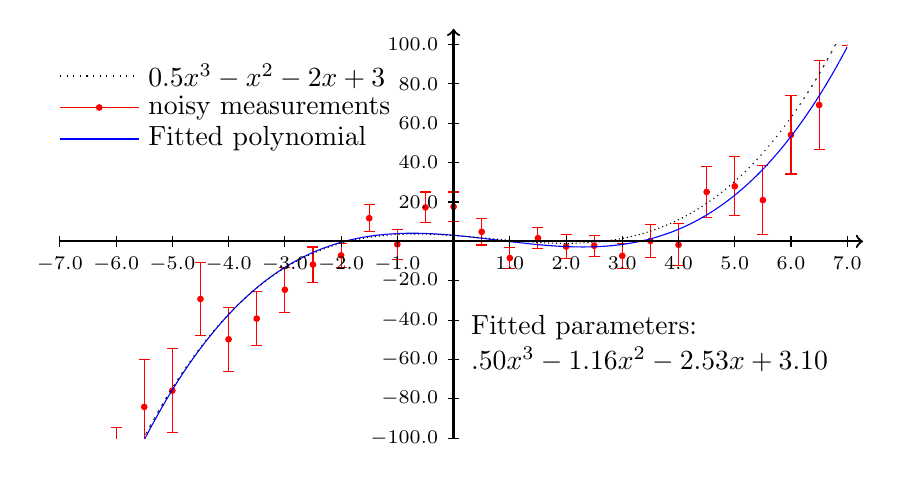
\begin{tikzpicture}
\begin{scope}[]
\clip (0,0) rectangle (10,5);
\draw[draw=red,fill=red] (-2.142857,-13.690766900522135) -- (-2.142857,-11.088684470629271);
\draw[draw=red,fill=red] (-2.142857,-12.389725685575703) circle(1pt); 
\draw[draw=red,fill=red] (-2.142857cm -2pt,-13.690766900522135) -- (-2.142857cm + 2pt,-13.690766900522135);
\draw[draw=red,fill=red] (-2.142857cm -2pt,-11.088684470629271) -- (-2.142857cm + 2pt,-11.088684470629271);
\draw[draw=red,fill=red] (-1.7857143,-11.547360643679772) -- (-1.7857143,-9.118151142533682);
\draw[draw=red,fill=red] (-1.7857143,-10.332755893106727) circle(1pt); 
\draw[draw=red,fill=red] (-1.7857143cm -2pt,-11.547360643679772) -- (-1.7857143cm + 2pt,-11.547360643679772);
\draw[draw=red,fill=red] (-1.7857143cm -2pt,-9.118151142533682) -- (-1.7857143cm + 2pt,-9.118151142533682);
\draw[draw=red,fill=red] (-1.4285715,-9.64862972900496) -- (-1.4285715,-7.388289951201308);
\draw[draw=red,fill=red] (-1.4285715,-8.518459840103134) circle(1pt); 
\draw[draw=red,fill=red] (-1.4285715cm -2pt,-9.64862972900496) -- (-1.4285715cm + 2pt,-9.64862972900496);
\draw[draw=red,fill=red] (-1.4285715cm -2pt,-7.388289951201308) -- (-1.4285715cm + 2pt,-7.388289951201308);
\draw[draw=red,fill=red] (-1.0714285,-7.637085601637203) -- (-1.0714285,-5.5415315929104665);
\draw[draw=red,fill=red] (-1.0714285,-6.589308597273835) circle(1pt); 
\draw[draw=red,fill=red] (-1.0714285cm -2pt,-7.637085601637203) -- (-1.0714285cm + 2pt,-7.637085601637203);
\draw[draw=red,fill=red] (-1.0714285cm -2pt,-5.5415315929104665) -- (-1.0714285cm + 2pt,-5.5415315929104665);
\draw[draw=red,fill=red] (-0.71428573,-4.594043342574411) -- (-0.71428573,-2.659108185284664);
\draw[draw=red,fill=red] (-0.71428573,-3.6265757639295373) circle(1pt); 
\draw[draw=red,fill=red] (-0.71428573cm -2pt,-4.594043342574411) -- (-0.71428573cm + 2pt,-4.594043342574411);
\draw[draw=red,fill=red] (-0.71428573cm -2pt,-2.659108185284664) -- (-0.71428573cm + 2pt,-2.659108185284664);
\draw[draw=red,fill=red] (-0.35714287,-5.796105953276756) -- (-0.35714287,-4.017538564788067);
\draw[draw=red,fill=red] (-0.35714287,-4.9068222590324115) circle(1pt); 
\draw[draw=red,fill=red] (-0.35714287cm -2pt,-5.796105953276756) -- (-0.35714287cm + 2pt,-5.796105953276756);
\draw[draw=red,fill=red] (-0.35714287cm -2pt,-4.017538564788067) -- (-0.35714287cm + 2pt,-4.017538564788067);
\draw[draw=red,fill=red] (0.0,-2.962409254330664) -- (0.0,-1.335874992561954);
\draw[draw=red,fill=red] (0.0,-2.149142123446309) circle(1pt); 
\draw[draw=red,fill=red] (0.0cm -2pt,-2.962409254330664) -- (0.0cm + 2pt,-2.962409254330664);
\draw[draw=red,fill=red] (0.0cm -2pt,-1.335874992561954) -- (0.0cm + 2pt,-1.335874992561954);
\draw[draw=red,fill=red] (0.35714287,-2.3595412915979326) -- (0.35714287,-0.8806257353550662);
\draw[draw=red,fill=red] (0.35714287,-1.6200835134764993) circle(1pt); 
\draw[draw=red,fill=red] (0.35714287cm -2pt,-2.3595412915979326) -- (0.35714287cm + 2pt,-2.3595412915979326);
\draw[draw=red,fill=red] (0.35714287cm -2pt,-0.8806257353550662) -- (0.35714287cm + 2pt,-0.8806257353550662);
\draw[draw=red,fill=red] (0.71428573,-1.199661460258557) -- (0.71428573,0.13612020890149779);
\draw[draw=red,fill=red] (0.71428573,-0.5317706256785296) circle(1pt); 
\draw[draw=red,fill=red] (0.71428573cm -2pt,-1.199661460258557) -- (0.71428573cm + 2pt,-1.199661460258557);
\draw[draw=red,fill=red] (0.71428573cm -2pt,0.13612020890149779) -- (0.71428573cm + 2pt,0.13612020890149779);
\draw[draw=red,fill=red] (1.0714285,-0.20121218473837588) -- (1.0714285,0.9959713490205806);
\draw[draw=red,fill=red] (1.0714285,0.39737958214110236) circle(1pt); 
\draw[draw=red,fill=red] (1.0714285cm -2pt,-0.20121218473837588) -- (1.0714285cm + 2pt,-0.20121218473837588);
\draw[draw=red,fill=red] (1.0714285cm -2pt,0.9959713490205806) -- (1.0714285cm + 2pt,0.9959713490205806);
\draw[draw=red,fill=red] (1.4285715,0.07283499514594083) -- (1.4285715,1.1359688202275442);
\draw[draw=red,fill=red] (1.4285715,0.6044019076867425) circle(1pt); 
\draw[draw=red,fill=red] (1.4285715cm -2pt,0.07283499514594083) -- (1.4285715cm + 2pt,0.07283499514594083);
\draw[draw=red,fill=red] (1.4285715cm -2pt,1.1359688202275442) -- (1.4285715cm + 2pt,1.1359688202275442);
\draw[draw=red,fill=red] (1.7857143,1.3014636063312879) -- (1.7857143,2.2350336438873484);
\draw[draw=red,fill=red] (1.7857143,1.7682486251093181) circle(1pt); 
\draw[draw=red,fill=red] (1.7857143cm -2pt,1.3014636063312879) -- (1.7857143cm + 2pt,1.3014636063312879);
\draw[draw=red,fill=red] (1.7857143cm -2pt,2.2350336438873484) -- (1.7857143cm + 2pt,2.2350336438873484);
\draw[draw=red,fill=red] (2.142857,0.8525355883035404) -- (2.142857,1.6608118413333621);
\draw[draw=red,fill=red] (2.142857,1.2566737148184512) circle(1pt); 
\draw[draw=red,fill=red] (2.142857cm -2pt,0.8525355883035404) -- (2.142857cm + 2pt,0.8525355883035404);
\draw[draw=red,fill=red] (2.142857cm -2pt,1.6608118413333621) -- (2.142857cm + 2pt,1.6608118413333621);
\draw[draw=red,fill=red] (2.5,1.1758875509572513) -- (2.5,1.8625856093055457);
\draw[draw=red,fill=red] (2.5,1.5192365801313985) circle(1pt); 
\draw[draw=red,fill=red] (2.5cm -2pt,1.1758875509572513) -- (2.5cm + 2pt,1.1758875509572513);
\draw[draw=red,fill=red] (2.5cm -2pt,1.8625856093055457) -- (2.5cm + 2pt,1.8625856093055457);
\draw[draw=red,fill=red] (2.857143,1.6017864499030297) -- (2.857143,2.169209911320506);
\draw[draw=red,fill=red] (2.857143,1.8854981806117679) circle(1pt); 
\draw[draw=red,fill=red] (2.857143cm -2pt,1.6017864499030297) -- (2.857143cm + 2pt,1.6017864499030297);
\draw[draw=red,fill=red] (2.857143cm -2pt,2.169209911320506) -- (2.857143cm + 2pt,2.169209911320506);
\draw[draw=red,fill=red] (3.2142859,1.9826782299002694) -- (3.2142859,2.428899674945172);
\draw[draw=red,fill=red] (3.2142859,2.2057889524227208) circle(1pt); 
\draw[draw=red,fill=red] (3.2142859cm -2pt,1.9826782299002694) -- (3.2142859cm + 2pt,1.9826782299002694);
\draw[draw=red,fill=red] (3.2142859cm -2pt,2.428899674945172) -- (3.2142859cm + 2pt,2.428899674945172);
\draw[draw=red,fill=red] (3.5714285,2.1719053314991754) -- (3.5714285,2.4719053314991752);
\draw[draw=red,fill=red] (3.5714285,2.3219053314991753) circle(1pt); 
\draw[draw=red,fill=red] (3.5714285cm -2pt,2.1719053314991754) -- (3.5714285cm + 2pt,2.1719053314991754);
\draw[draw=red,fill=red] (3.5714285cm -2pt,2.4719053314991752) -- (3.5714285cm + 2pt,2.4719053314991752);
\draw[draw=red,fill=red] (3.9285715,2.622904496231831) -- (3.9285715,2.9665185623952812);
\draw[draw=red,fill=red] (3.9285715,2.794711529313556) circle(1pt); 
\draw[draw=red,fill=red] (3.9285715cm -2pt,2.622904496231831) -- (3.9285715cm + 2pt,2.622904496231831);
\draw[draw=red,fill=red] (3.9285715cm -2pt,2.9665185623952812) -- (3.9285715cm + 2pt,2.9665185623952812);
\draw[draw=red,fill=red] (4.285714,2.268574659499892) -- (4.285714,2.6556575288385895);
\draw[draw=red,fill=red] (4.285714,2.462116094169241) circle(1pt); 
\draw[draw=red,fill=red] (4.285714cm -2pt,2.268574659499892) -- (4.285714cm + 2pt,2.268574659499892);
\draw[draw=red,fill=red] (4.285714cm -2pt,2.6556575288385895) -- (4.285714cm + 2pt,2.6556575288385895);
\draw[draw=red,fill=red] (4.642857,2.7353486391801107) -- (4.642857,3.127377282876826);
\draw[draw=red,fill=red] (4.642857,2.9313629610284684) circle(1pt); 
\draw[draw=red,fill=red] (4.642857cm -2pt,2.7353486391801107) -- (4.642857cm + 2pt,2.7353486391801107);
\draw[draw=red,fill=red] (4.642857cm -2pt,3.127377282876826) -- (4.642857cm + 2pt,3.127377282876826);
\draw[draw=red,fill=red] (5.0,2.753229322304523) -- (5.0,3.126434403061411);
\draw[draw=red,fill=red] (5.0,2.939831862682967) circle(1pt); 
\draw[draw=red,fill=red] (5.0cm -2pt,2.753229322304523) -- (5.0cm + 2pt,2.753229322304523);
\draw[draw=red,fill=red] (5.0cm -2pt,3.126434403061411) -- (5.0cm + 2pt,3.126434403061411);
\draw[draw=red,fill=red] (5.357143,2.4538980485227913) -- (5.357143,2.788527168701154);
\draw[draw=red,fill=red] (5.357143,2.6212126086119727) circle(1pt); 
\draw[draw=red,fill=red] (5.357143cm -2pt,2.4538980485227913) -- (5.357143cm + 2pt,2.4538980485227913);
\draw[draw=red,fill=red] (5.357143cm -2pt,2.788527168701154) -- (5.357143cm + 2pt,2.788527168701154);
\draw[draw=red,fill=red] (5.714286,2.152866155952158) -- (5.714286,2.4235768340708126);
\draw[draw=red,fill=red] (5.714286,2.288221495011485) circle(1pt); 
\draw[draw=red,fill=red] (5.714286cm -2pt,2.152866155952158) -- (5.714286cm + 2pt,2.152866155952158);
\draw[draw=red,fill=red] (5.714286cm -2pt,2.4235768340708126) -- (5.714286cm + 2pt,2.4235768340708126);
\draw[draw=red,fill=red] (6.071429,2.404394903388126) -- (6.071429,2.6793949033881264);
\draw[draw=red,fill=red] (6.071429,2.541894903388126) circle(1pt); 
\draw[draw=red,fill=red] (6.071429cm -2pt,2.404394903388126) -- (6.071429cm + 2pt,2.404394903388126);
\draw[draw=red,fill=red] (6.071429cm -2pt,2.6793949033881264) -- (6.071429cm + 2pt,2.6793949033881264);
\draw[draw=red,fill=red] (6.4285717,2.2844725706941964) -- (6.4285717,2.5844725706941962);
\draw[draw=red,fill=red] (6.4285717,2.4344725706941963) circle(1pt); 
\draw[draw=red,fill=red] (6.4285717cm -2pt,2.2844725706941964) -- (6.4285717cm + 2pt,2.2844725706941964);
\draw[draw=red,fill=red] (6.4285717cm -2pt,2.5844725706941962) -- (6.4285717cm + 2pt,2.5844725706941962);
\draw[draw=red,fill=red] (6.7857146,2.311012057325212) -- (6.7857146,2.5771558401018266);
\draw[draw=red,fill=red] (6.7857146,2.4440839487135193) circle(1pt); 
\draw[draw=red,fill=red] (6.7857146cm -2pt,2.311012057325212) -- (6.7857146cm + 2pt,2.311012057325212);
\draw[draw=red,fill=red] (6.7857146cm -2pt,2.5771558401018266) -- (6.7857146cm + 2pt,2.5771558401018266);
\draw[draw=red,fill=red] (7.142857,2.1554091573639695) -- (7.142857,2.4778836445031285);
\draw[draw=red,fill=red] (7.142857,2.316646400933549) circle(1pt); 
\draw[draw=red,fill=red] (7.142857cm -2pt,2.1554091573639695) -- (7.142857cm + 2pt,2.1554091573639695);
\draw[draw=red,fill=red] (7.142857cm -2pt,2.4778836445031285) -- (7.142857cm + 2pt,2.4778836445031285);
\draw[draw=red,fill=red] (7.5,2.2919468922135207) -- (7.5,2.7197077316921283);
\draw[draw=red,fill=red] (7.5,2.5058273119528245) circle(1pt); 
\draw[draw=red,fill=red] (7.5cm -2pt,2.2919468922135207) -- (7.5cm + 2pt,2.2919468922135207);
\draw[draw=red,fill=red] (7.5cm -2pt,2.7197077316921283) -- (7.5cm + 2pt,2.7197077316921283);
\draw[draw=red,fill=red] (7.857143,2.190573053492995) -- (7.857143,2.722235532528535);
\draw[draw=red,fill=red] (7.857143,2.456404293010765) circle(1pt); 
\draw[draw=red,fill=red] (7.857143cm -2pt,2.190573053492995) -- (7.857143cm + 2pt,2.190573053492995);
\draw[draw=red,fill=red] (7.857143cm -2pt,2.722235532528535) -- (7.857143cm + 2pt,2.722235532528535);
\draw[draw=red,fill=red] (8.214286,2.807793977537827) -- (8.214286,3.447253873319001);
\draw[draw=red,fill=red] (8.214286,3.127523925428414) circle(1pt); 
\draw[draw=red,fill=red] (8.214286cm -2pt,2.807793977537827) -- (8.214286cm + 2pt,2.807793977537827);
\draw[draw=red,fill=red] (8.214286cm -2pt,3.447253873319001) -- (8.214286cm + 2pt,3.447253873319001);
\draw[draw=red,fill=red] (8.571428,2.8235369533398798) -- (8.571428,3.5758050041992426);
\draw[draw=red,fill=red] (8.571428,3.199670978769561) circle(1pt); 
\draw[draw=red,fill=red] (8.571428cm -2pt,2.8235369533398798) -- (8.571428cm + 2pt,2.8235369533398798);
\draw[draw=red,fill=red] (8.571428cm -2pt,3.5758050041992426) -- (8.571428cm + 2pt,3.5758050041992426);
\draw[draw=red,fill=red] (8.928572,2.5894682162756566) -- (8.928572,3.459822600165253);
\draw[draw=red,fill=red] (8.928572,3.024645408220455) circle(1pt); 
\draw[draw=red,fill=red] (8.928572cm -2pt,2.5894682162756566) -- (8.928572cm + 2pt,2.5894682162756566);
\draw[draw=red,fill=red] (8.928572cm -2pt,3.459822600165253) -- (8.928572cm + 2pt,3.459822600165253);
\draw[draw=red,fill=red] (9.285714,3.3555610683946355) -- (9.285714,4.349286461714013);
\draw[draw=red,fill=red] (9.285714,3.8524237650543243) circle(1pt); 
\draw[draw=red,fill=red] (9.285714cm -2pt,3.3555610683946355) -- (9.285714cm + 2pt,3.3555610683946355);
\draw[draw=red,fill=red] (9.285714cm -2pt,4.349286461714013) -- (9.285714cm + 2pt,4.349286461714013);
\draw[draw=red,fill=red] (9.642858,3.670924469182596) -- (9.642858,4.793217806467432);
\draw[draw=red,fill=red] (9.642858,4.232071137825014) circle(1pt); 
\draw[draw=red,fill=red] (9.642858cm -2pt,3.670924469182596) -- (9.642858cm + 2pt,3.670924469182596);
\draw[draw=red,fill=red] (9.642858cm -2pt,4.793217806467432) -- (9.642858cm + 2pt,4.793217806467432);
\draw[draw=red,fill=red] (10.0,4.987673323439317) -- (10.0,6.24360892753646);
\draw[draw=red,fill=red] (10.0,5.615641125487889) circle(1pt); 
\draw[draw=red,fill=red] (10.0cm -2pt,4.987673323439317) -- (10.0cm + 2pt,4.987673323439317);
\draw[draw=red,fill=red] (10.0cm -2pt,6.24360892753646) -- (10.0cm + 2pt,6.24360892753646);
\draw[draw=red,fill=red] (10.357143,4.515341770846103) -- (10.357143,5.909860502386131);
\draw[draw=red,fill=red] (10.357143,5.212601136616117) circle(1pt); 
\draw[draw=red,fill=red] (10.357143cm -2pt,4.515341770846103) -- (10.357143cm + 2pt,4.515341770846103);
\draw[draw=red,fill=red] (10.357143cm -2pt,5.909860502386131) -- (10.357143cm + 2pt,5.909860502386131);
\draw[draw=red,fill=red] (10.714286,6.270108949441174) -- (10.714286,7.808017765467139);
\draw[draw=red,fill=red] (10.714286,7.039063357454157) circle(1pt); 
\draw[draw=red,fill=red] (10.714286cm -2pt,6.270108949441174) -- (10.714286cm + 2pt,6.270108949441174);
\draw[draw=red,fill=red] (10.714286cm -2pt,7.808017765467139) -- (10.714286cm + 2pt,7.808017765467139);
\draw[draw=red,fill=red] (11.071428,8.310451887182419) -- (11.071428,9.996427997353775);
\draw[draw=red,fill=red] (11.071428,9.153439942268097) circle(1pt); 
\draw[draw=red,fill=red] (11.071428cm -2pt,8.310451887182419) -- (11.071428cm + 2pt,8.310451887182419);
\draw[draw=red,fill=red] (11.071428cm -2pt,9.996427997353775) -- (11.071428cm + 2pt,9.996427997353775);
\draw[draw=red,fill=red] (11.428572,7.494686295042708) -- (11.428572,9.333283255860103);
\draw[draw=red,fill=red] (11.428572,8.413984775451405) circle(1pt); 
\draw[draw=red,fill=red] (11.428572cm -2pt,7.494686295042708) -- (11.428572cm + 2pt,7.494686295042708);
\draw[draw=red,fill=red] (11.428572cm -2pt,9.333283255860103) -- (11.428572cm + 2pt,9.333283255860103);
\draw[draw=red,fill=red] (11.785714,7.12076876638811) -- (11.785714,9.116423243173664);
\draw[draw=red,fill=red] (11.785714,8.118596004780887) circle(1pt); 
\draw[draw=red,fill=red] (11.785714cm -2pt,7.12076876638811) -- (11.785714cm + 2pt,7.12076876638811);
\draw[draw=red,fill=red] (11.785714cm -2pt,9.116423243173664) -- (11.785714cm + 2pt,9.116423243173664);
\draw[draw=red,fill=red] (12.142858,11.084758723728982) -- (12.142858,13.241797302807075);
\draw[draw=red,fill=red] (12.142858,12.163278013268028) circle(1pt); 
\draw[draw=red,fill=red] (12.142858cm -2pt,11.084758723728982) -- (12.142858cm + 2pt,11.084758723728982);
\draw[draw=red,fill=red] (12.142858cm -2pt,13.241797302807075) -- (12.142858cm + 2pt,13.241797302807075);
\begin{scope}[blue]
\draw[] (0.0,-2.6659163637589467) -- (0.05,-2.5154258388318347);
\draw[] (0.05,-2.5154258388318347) -- (0.1,-2.367751397701819);
\draw[] (0.1,-2.367751397701819) -- (0.15,-2.222867474803506);
\draw[] (0.15,-2.222867474803506) -- (0.2,-2.0807485045715);
\draw[] (0.2,-2.0807485045715) -- (0.25,-1.9413689214404137);
\draw[] (0.25,-1.9413689214404137) -- (0.3,-1.8047031598448484);
\draw[] (0.3,-1.8047031598448484) -- (0.35,-1.670725654219415);
\draw[] (0.35,-1.670725654219415) -- (0.4,-1.5394108389987224);
\draw[] (0.4,-1.5394108389987224) -- (0.45,-1.4107331486173735);
\draw[] (0.45,-1.4107331486173735) -- (0.5,-1.2846670175099775);
\draw[] (0.5,-1.2846670175099775) -- (0.55,-1.1611868801111414);
\draw[] (0.55,-1.1611868801111414) -- (0.6,-1.0402671708554727);
\draw[] (0.6,-1.0402671708554727) -- (0.65,-0.9218823241775788);
\draw[] (0.65,-0.9218823241775788) -- (0.7,-0.8060067745120669);
\draw[] (0.7,-0.8060067745120669) -- (0.75,-0.6926149562935446);
\draw[] (0.75,-0.6926149562935446) -- (0.8,-0.5816813039566181);
\draw[] (0.8,-0.5816813039566181) -- (0.85,-0.4731802519358951);
\draw[] (0.85,-0.4731802519358951) -- (0.9,-0.36708623466598456);
\draw[] (0.9,-0.36708623466598456) -- (0.95,-0.2633736865814903);
\draw[] (0.95,-0.2633736865814903) -- (1.0,-0.16201704211702186);
\draw[] (1.0,-0.16201704211702186) -- (1.05,-0.06299073570718754);
\draw[] (1.05,-0.06299073570718754) -- (1.1,0.03373079821340852);
\draw[] (1.1,0.03373079821340852) -- (1.15,0.12817312521015686);
\draw[] (1.15,0.12817312521015686) -- (1.2,0.2203618108484502);
\draw[] (1.2,0.2203618108484502) -- (1.25,0.31032242069368293);
\draw[] (1.25,0.31032242069368293) -- (1.3,0.39808052031124674);
\draw[] (1.3,0.39808052031124674) -- (1.35,0.4836616752665332);
\draw[] (1.35,0.4836616752665332) -- (1.4,0.5670914511249375);
\draw[] (1.4,0.5670914511249375) -- (1.45,0.6483954134518509);
\draw[] (1.45,0.6483954134518509) -- (1.5,0.7275991278126653);
\draw[] (1.5,0.7275991278126653) -- (1.55,0.8047281597727757);
\draw[] (1.55,0.8047281597727757) -- (1.6,0.8798080748975738);
\draw[] (1.6,0.8798080748975738) -- (1.65,0.9528644387524512);
\draw[] (1.65,0.9528644387524512) -- (1.7,1.0239228169028025);
\draw[] (1.7,1.0239228169028025) -- (1.75,1.09300877491402);
\draw[] (1.75,1.09300877491402) -- (1.8,1.160147878351495);
\draw[] (1.8,1.160147878351495) -- (1.85,1.2253656927806218);
\draw[] (1.85,1.2253656927806218) -- (1.9,1.2886877837667936);
\draw[] (1.9,1.2886877837667936) -- (1.95,1.3501397168754017);
\draw[] (1.95,1.3501397168754017) -- (2.0,1.4097470576718387);
\draw[] (2.0,1.4097470576718387) -- (2.05,1.4675353717214985);
\draw[] (2.05,1.4675353717214985) -- (2.1,1.5235302245897737);
\draw[] (2.1,1.5235302245897737) -- (2.15,1.577757181842056);
\draw[] (2.15,1.577757181842056) -- (2.2,1.6302418090437396);
\draw[] (2.2,1.6302418090437396) -- (2.25,1.681009671760216);
\draw[] (2.25,1.681009671760216) -- (2.3,1.730086335556879);
\draw[] (2.3,1.730086335556879) -- (2.35,1.7774973659991204);
\draw[] (2.35,1.7774973659991204) -- (2.4,1.8232683286523337);
\draw[] (2.4,1.8232683286523337) -- (2.45,1.8674247890819113);
\draw[] (2.45,1.8674247890819113) -- (2.5,1.9099923128532459);
\draw[] (2.5,1.9099923128532459) -- (2.55,1.9509964655317305);
\draw[] (2.55,1.9509964655317305) -- (2.6,1.990462812682758);
\draw[] (2.6,1.990462812682758) -- (2.65,2.02841691987172);
\draw[] (2.65,2.02841691987172) -- (2.7,2.0648843526640106);
\draw[] (2.7,2.0648843526640106) -- (2.75,2.099890676625022);
\draw[] (2.75,2.099890676625022) -- (2.8,2.1334614573201476);
\draw[] (2.8,2.1334614573201476) -- (2.85,2.165622260314779);
\draw[] (2.85,2.165622260314779) -- (2.9,2.1963986511743094);
\draw[] (2.9,2.1963986511743094) -- (2.95,2.2258161954641316);
\draw[] (2.95,2.2258161954641316) -- (3.0,2.2539004587496385);
\draw[] (3.0,2.2539004587496385) -- (3.05,2.2806770065962225);
\draw[] (3.05,2.2806770065962225) -- (3.1,2.306171404569277);
\draw[] (3.1,2.306171404569277) -- (3.15,2.3304092182341942);
\draw[] (3.15,2.3304092182341942) -- (3.2,2.3534160131563673);
\draw[] (3.2,2.3534160131563673) -- (3.25,2.375217354901188);
\draw[] (3.25,2.375217354901188) -- (3.3,2.3958388090340508);
\draw[] (3.3,2.3958388090340508) -- (3.35,2.415305941120347);
\draw[] (3.35,2.415305941120347) -- (3.4,2.4336443167254695);
\draw[] (3.4,2.4336443167254695) -- (3.45,2.4508795014148115);
\draw[] (3.45,2.4508795014148115) -- (3.5,2.467037060753766);
\draw[] (3.5,2.467037060753766) -- (3.55,2.4821425603077247);
\draw[] (3.55,2.4821425603077247) -- (3.6,2.4962215656420814);
\draw[] (3.6,2.4962215656420814) -- (3.65,2.5092996423222287);
\draw[] (3.65,2.5092996423222287) -- (3.7,2.5214023559135588);
\draw[] (3.7,2.5214023559135588) -- (3.75,2.5325552719814644);
\draw[] (3.75,2.5325552719814644) -- (3.8,2.542783956091339);
\draw[] (3.8,2.542783956091339) -- (3.85,2.552113973808575);
\draw[] (3.85,2.552113973808575) -- (3.9,2.560570890698565);
\draw[] (3.9,2.560570890698565) -- (3.95,2.568180272326702);
\draw[] (3.95,2.568180272326702) -- (4.0,2.574967684258378);
\draw[] (4.0,2.574967684258378) -- (4.05,2.580958692058987);
\draw[] (4.05,2.580958692058987) -- (4.1,2.586178861293921);
\draw[] (4.1,2.586178861293921) -- (4.15,2.5906537575285724);
\draw[] (4.15,2.5906537575285724) -- (4.2,2.5944089463283353);
\draw[] (4.2,2.5944089463283353) -- (4.25,2.5974699932586005);
\draw[] (4.25,2.5974699932586005) -- (4.3,2.5998624638847625);
\draw[] (4.3,2.5998624638847625) -- (4.35,2.601611923772213);
\draw[] (4.35,2.601611923772213) -- (4.4,2.6027439384863458);
\draw[] (4.4,2.6027439384863458) -- (4.45,2.603284073592552);
\draw[] (4.45,2.603284073592552) -- (4.5,2.6032578946562257);
\draw[] (4.5,2.6032578946562257) -- (4.55,2.602690967242759);
\draw[] (4.55,2.602690967242759) -- (4.6,2.6016088569175455);
\draw[] (4.6,2.6016088569175455) -- (4.65,2.600037129245977);
\draw[] (4.65,2.600037129245977) -- (4.7,2.5980013497934467);
\draw[] (4.7,2.5980013497934467) -- (4.75,2.5955270841253473);
\draw[] (4.75,2.5955270841253473) -- (4.8,2.592639897807071);
\draw[] (4.8,2.592639897807071) -- (4.85,2.589365356404012);
\draw[] (4.85,2.589365356404012) -- (4.9,2.5857290254815615);
\draw[] (4.9,2.5857290254815615) -- (4.95,2.5817564706051126);
\draw[] (4.95,2.5817564706051126) -- (5.0,2.577473257340059);
\draw[] (5.0,2.577473257340059) -- (5.05,2.5729049512517923);
\draw[] (5.05,2.5729049512517923) -- (5.1,2.5680771179057054);
\draw[] (5.1,2.5680771179057054) -- (5.15,2.5630153228671917);
\draw[] (5.15,2.5630153228671917) -- (5.2,2.557745131701644);
\draw[] (5.2,2.557745131701644) -- (5.25,2.552292109974454);
\draw[] (5.25,2.552292109974454) -- (5.3,2.5466818232510153);
\draw[] (5.3,2.5466818232510153) -- (5.35,2.5409398370967207);
\draw[] (5.35,2.5409398370967207) -- (5.4,2.5350917170769627);
\draw[] (5.4,2.5350917170769627) -- (5.45,2.5291630287571336);
\draw[] (5.45,2.5291630287571336) -- (5.5,2.523179337702627);
\draw[] (5.5,2.523179337702627) -- (5.55,2.517166209478835);
\draw[] (5.55,2.517166209478835) -- (5.6,2.511149209651151);
\draw[] (5.6,2.511149209651151) -- (5.65,2.5051539037849673);
\draw[] (5.65,2.5051539037849673) -- (5.7,2.499205857445676);
\draw[] (5.7,2.499205857445676) -- (5.75,2.493330636198672);
\draw[] (5.75,2.493330636198672) -- (5.8,2.4875538056093456);
\draw[] (5.8,2.4875538056093456) -- (5.85,2.48190093124309);
\draw[] (5.85,2.48190093124309) -- (5.9,2.4763975786652996);
\draw[] (5.9,2.4763975786652996) -- (5.95,2.4710693134413657);
\draw[] (5.95,2.4710693134413657) -- (6.0,2.465941701136681);
\draw[] (6.0,2.465941701136681) -- (6.05,2.4610403073166394);
\draw[] (6.05,2.4610403073166394) -- (6.1,2.4563906975466323);
\draw[] (6.1,2.4563906975466323) -- (6.15,2.452018437392053);
\draw[] (6.15,2.452018437392053) -- (6.2,2.4479490924182947);
\draw[] (6.2,2.4479490924182947) -- (6.25,2.4442082281907496);
\draw[] (6.25,2.4442082281907496) -- (6.3,2.4408214102748107);
\draw[] (6.3,2.4408214102748107) -- (6.35,2.437814204235871);
\draw[] (6.35,2.437814204235871) -- (6.4,2.435212175639322);
\draw[] (6.4,2.435212175639322) -- (6.45,2.433040890050558);
\draw[] (6.45,2.433040890050558) -- (6.5,2.431325913034971);
\draw[] (6.5,2.431325913034971) -- (6.55,2.4300928101579538);
\draw[] (6.55,2.4300928101579538) -- (6.6,2.429367146984899);
\draw[] (6.6,2.429367146984899) -- (6.65,2.4291744890811997);
\draw[] (6.65,2.4291744890811997) -- (6.7,2.429540402012249);
\draw[] (6.7,2.429540402012249) -- (6.75,2.430490451343439);
\draw[] (6.75,2.430490451343439) -- (6.8,2.432050202640162);
\draw[] (6.8,2.432050202640162) -- (6.85,2.434245221467812);
\draw[] (6.85,2.434245221467812) -- (6.9,2.437101073391781);
\draw[] (6.9,2.437101073391781) -- (6.95,2.4406433239774614);
\draw[] (6.95,2.4406433239774614) -- (7.0,2.4448975387902463);
\draw[] (7.0,2.4448975387902463) -- (7.05,2.449889283395529);
\draw[] (7.05,2.449889283395529) -- (7.1,2.455644123358702);
\draw[] (7.1,2.455644123358702) -- (7.15,2.462187624245158);
\draw[] (7.15,2.462187624245158) -- (7.2,2.469545351620289);
\draw[] (7.2,2.469545351620289) -- (7.25,2.4777428710494886);
\draw[] (7.25,2.4777428710494886) -- (7.3,2.486805748098149);
\draw[] (7.3,2.486805748098149) -- (7.35,2.496759548331664);
\draw[] (7.35,2.496759548331664) -- (7.4,2.5076298373154247);
\draw[] (7.4,2.5076298373154247) -- (7.45,2.5194421806148255);
\draw[] (7.45,2.5194421806148255) -- (7.5,2.5322221437952583);
\draw[] (7.5,2.5322221437952583) -- (7.55,2.5459952924221154);
\draw[] (7.55,2.5459952924221154) -- (7.6,2.5607871920607908);
\draw[] (7.6,2.5607871920607908) -- (7.65,2.5766234082766766);
\draw[] (7.65,2.5766234082766766) -- (7.7,2.593529506635165);
\draw[] (7.7,2.593529506635165) -- (7.75,2.6115310527016495);
\draw[] (7.75,2.6115310527016495) -- (7.8,2.630653612041523);
\draw[] (7.8,2.630653612041523) -- (7.85,2.650922750220177);
\draw[] (7.85,2.650922750220177) -- (7.9,2.6723640328030056);
\draw[] (7.9,2.6723640328030056) -- (7.95,2.6950030253554007);
\draw[] (7.95,2.6950030253554007) -- (8.0,2.7188652934427564);
\draw[] (8.0,2.7188652934427564) -- (8.05,2.743976402630463);
\draw[] (8.05,2.743976402630463) -- (8.1,2.7703619184839154);
\draw[] (8.1,2.7703619184839154) -- (8.15,2.7980474065685064);
\draw[] (8.15,2.7980474065685064) -- (8.2,2.8270584324496277);
\draw[] (8.2,2.8270584324496277) -- (8.25,2.8574205616926713);
\draw[] (8.25,2.8574205616926713) -- (8.3,2.889159359863032);
\draw[] (8.3,2.889159359863032) -- (8.35,2.9223003925261017);
\draw[] (8.35,2.9223003925261017) -- (8.4,2.956869225247272);
\draw[] (8.4,2.956869225247272) -- (8.45,2.9928914235919377);
\draw[] (8.45,2.9928914235919377) -- (8.5,3.0303925531254903);
\draw[] (8.5,3.0303925531254903) -- (8.55,3.069398179413322);
\draw[] (8.55,3.069398179413322) -- (8.6,3.1099338680208275);
\draw[] (8.6,3.1099338680208275) -- (8.65,3.152025184513398);
\draw[] (8.65,3.152025184513398) -- (8.7,3.1956976944564257);
\draw[] (8.7,3.1956976944564257) -- (8.75,3.240976963415305);
\draw[] (8.75,3.240976963415305) -- (8.8,3.2878885569554286);
\draw[] (8.8,3.2878885569554286) -- (8.85,3.3364580406421864);
\draw[] (8.85,3.3364580406421864) -- (8.9,3.386710980040976);
\draw[] (8.9,3.386710980040976) -- (8.95,3.4386729407171854);
\draw[] (8.95,3.4386729407171854) -- (9.0,3.4923694882362106);
\draw[] (9.0,3.4923694882362106) -- (9.05,3.5478261881634423);
\draw[] (9.05,3.5478261881634423) -- (9.1,3.6050686060642754);
\draw[] (9.1,3.6050686060642754) -- (9.15,3.6641223075041);
\draw[] (9.15,3.6641223075041) -- (9.2,3.7250128580483106);
\draw[] (9.2,3.7250128580483106) -- (9.25,3.7877658232623004);
\draw[] (9.25,3.7877658232623004) -- (9.3,3.8524067687114596);
\draw[] (9.3,3.8524067687114596) -- (9.35,3.918961259961185);
\draw[] (9.35,3.918961259961185) -- (9.4,3.987454862576866);
\draw[] (9.4,3.987454862576866) -- (9.45,4.057913142123896);
\draw[] (9.45,4.057913142123896) -- (9.5,4.130361664167667);
\draw[] (9.5,4.130361664167667) -- (9.55,4.204825994273575);
\draw[] (9.55,4.204825994273575) -- (9.6,4.28133169800701);
\draw[] (9.6,4.28133169800701) -- (9.65,4.359904340933364);
\draw[] (9.65,4.359904340933364) -- (9.7,4.440569488618033);
\draw[] (9.7,4.440569488618033) -- (9.75,4.523352706626407);
\draw[] (9.75,4.523352706626407) -- (9.8,4.608279560523878);
\draw[] (9.8,4.608279560523878) -- (9.85,4.695375615875845);
\draw[] (9.85,4.695375615875845) -- (9.9,4.784666438247692);
\draw[] (9.9,4.784666438247692) -- (9.95,4.876177593204816);
\draw[] (9.95,4.876177593204816) -- (10.0,4.969934646312612);
\end{scope}
\node[right] at (5.1,1.4) {Fitted parameters: };
\node[right] at (5.1,1.0) {$.50x^3 -1.16x^2 -2.53x +3.10$};
\begin{scope}[dotted]
\draw[] (0.0,-2.5875) -- (0.05,-2.439279131469726);
\draw[] (0.05,-2.439279131469726) -- (0.1,-2.293850717773437);
\draw[] (0.1,-2.293850717773437) -- (0.15,-2.1511880560302736);
\draw[] (0.15,-2.1511880560302736) -- (0.2,-2.011265206298828);
\draw[] (0.2,-2.011265206298828) -- (0.25,-1.8740577545166013);
\draw[] (0.25,-1.8740577545166013) -- (0.3,-1.739538616333008);
\draw[] (0.3,-1.739538616333008) -- (0.35,-1.607683759155273);
\draw[] (0.35,-1.607683759155273) -- (0.4,-1.478464954223633);
\draw[] (0.4,-1.478464954223633) -- (0.45,-1.3518577874755855);
\draw[] (0.45,-1.3518577874755855) -- (0.5,-1.227837844848633);
\draw[] (0.5,-1.227837844848633) -- (0.55,-1.1063770883178712);
\draw[] (0.55,-1.1063770883178712) -- (0.6,-0.9874511038208013);
\draw[] (0.6,-0.9874511038208013) -- (0.65,-0.8710341421508787);
\draw[] (0.65,-0.8710341421508787) -- (0.7,-0.7570998818969727);
\draw[] (0.7,-0.7570998818969727) -- (0.75,-0.6456231460571289);
\draw[] (0.75,-0.6456231460571289) -- (0.8,-0.5365785668945311);
\draw[] (0.8,-0.5365785668945311) -- (0.85,-0.429939250793457);
\draw[] (0.85,-0.429939250793457) -- (0.9,-0.3256800207519529);
\draw[] (0.9,-0.3256800207519529) -- (0.95,-0.22377569976806627);
\draw[] (0.95,-0.22377569976806627) -- (1.0,-0.12419996643066397);
\draw[] (1.0,-0.12419996643066397) -- (1.05,-0.026927453002929626);
\draw[] (1.05,-0.026927453002929626) -- (1.1,0.0680683526611329);
\draw[] (1.1,0.0680683526611329) -- (1.15,0.1608124368286134);
\draw[] (1.15,0.1608124368286134) -- (1.2,0.251330167236328);
\draw[] (1.2,0.251330167236328) -- (1.25,0.3396484375);
\draw[] (1.25,0.3396484375) -- (1.3,0.42579223388671894);
\draw[] (1.3,0.42579223388671894) -- (1.35,0.5097871148681641);
\draw[] (1.35,0.5097871148681641) -- (1.4,0.5916592111206054);
\draw[] (1.4,0.5916592111206054) -- (1.45,0.6714343672180177);
\draw[] (1.45,0.6714343672180177) -- (1.5,0.7491374740600584);
\draw[] (1.5,0.7491374740600584) -- (1.55,0.8247952345275877);
\draw[] (1.55,0.8247952345275877) -- (1.6,0.8984326348876952);
\draw[] (1.6,0.8984326348876952) -- (1.65,0.9700759965515136);
\draw[] (1.65,0.9700759965515136) -- (1.7,1.0397509733581543);
\draw[] (1.7,1.0397509733581543) -- (1.75,1.1074826469421386);
\draw[] (1.75,1.1074826469421386) -- (1.8,1.1732976248168945);
\draw[] (1.8,1.1732976248168945) -- (1.85,1.2372210839843751);
\draw[] (1.85,1.2372210839843751) -- (1.9,1.2992785829162599);
\draw[] (1.9,1.2992785829162599) -- (1.95,1.3594964430236816);
\draw[] (1.95,1.3594964430236816) -- (2.0,1.4179001274108887);
\draw[] (2.0,1.4179001274108887) -- (2.05,1.4745150038146972);
\draw[] (2.05,1.4745150038146972) -- (2.1,1.5293673936462402);
\draw[] (2.1,1.5293673936462402) -- (2.15,1.5824825215911864);
\draw[] (2.15,1.5824825215911864) -- (2.2,1.6338863275909425);
\draw[] (2.2,1.6338863275909425) -- (2.25,1.683604751586914);
\draw[] (2.25,1.683604751586914) -- (2.3,1.7316631136322023);
\draw[] (2.3,1.7316631136322023) -- (2.35,1.778087353668213);
\draw[] (2.35,1.778087353668213) -- (2.4,1.8229031732177734);
\draw[] (2.4,1.8229031732177734) -- (2.45,1.8661363691711426);
\draw[] (2.45,1.8661363691711426) -- (2.5,1.9078125);
\draw[] (2.5,1.9078125) -- (2.55,1.9479574102783204);
\draw[] (2.55,1.9479574102783204) -- (2.6,1.9865968492126462);
\draw[] (2.6,1.9865968492126462) -- (2.65,2.0237564229583738);
\draw[] (2.65,2.0237564229583738) -- (2.7,2.059461880722046);
\draw[] (2.7,2.059461880722046) -- (2.75,2.093739019393921);
\draw[] (2.75,2.093739019393921) -- (2.8,2.1266136120223997);
\draw[] (2.8,2.1266136120223997) -- (2.85,2.1581112647628786);
\draw[] (2.85,2.1581112647628786) -- (2.9,2.1882576791381836);
\draw[] (2.9,2.1882576791381836) -- (2.95,2.217078747406006);
\draw[] (2.95,2.217078747406006) -- (3.0,2.244600004196167);
\draw[] (3.0,2.244600004196167) -- (3.05,2.2708472940826416);
\draw[] (3.05,2.2708472940826416) -- (3.1,2.295846270904541);
\draw[] (3.1,2.295846270904541) -- (3.15,2.31962277923584);
\draw[] (3.15,2.31962277923584) -- (3.2,2.3422024013900757);
\draw[] (3.2,2.3422024013900757) -- (3.25,2.3636109342575073);
\draw[] (3.25,2.3636109342575073) -- (3.3,2.383874079360962);
\draw[] (3.3,2.383874079360962) -- (3.35,2.403017621669769);
\draw[] (3.35,2.403017621669769) -- (3.4,2.421067203102112);
\draw[] (3.4,2.421067203102112) -- (3.45,2.4380485728645325);
\draw[] (3.45,2.4380485728645325) -- (3.5,2.4539875159263613);
\draw[] (3.5,2.4539875159263613) -- (3.55,2.46890967420578);
\draw[] (3.55,2.46890967420578) -- (3.6,2.4828407909488677);
\draw[] (3.6,2.4828407909488677) -- (3.65,2.4958066392040252);
\draw[] (3.65,2.4958066392040252) -- (3.7,2.507832896652222);
\draw[] (3.7,2.507832896652222) -- (3.75,2.5189453125);
\draw[] (3.75,2.5189453125) -- (3.8,2.529169606151581);
\draw[] (3.8,2.529169606151581) -- (3.85,2.538531485090256);
\draw[] (3.85,2.538531485090256) -- (3.9,2.5470567015028);
\draw[] (3.9,2.5470567015028) -- (3.95,2.5547709598922728);
\draw[] (3.95,2.5547709598922728) -- (4.0,2.561700000524521);
\draw[] (4.0,2.561700000524521) -- (4.05,2.5678695338630675);
\draw[] (4.05,2.5678695338630675) -- (4.1,2.5733053001737596);
\draw[] (4.1,2.5733053001737596) -- (4.15,2.5780330099201203);
\draw[] (4.15,2.5780330099201203) -- (4.2,2.582078400387764);
\draw[] (4.2,2.582078400387764) -- (4.25,2.585467189490795);
\draw[] (4.25,2.585467189490795) -- (4.3,2.5882250988686084);
\draw[] (4.3,2.5882250988686084) -- (4.35,2.5903778620815276);
\draw[] (4.35,2.5903778620815276) -- (4.4,2.5919512007689476);
\draw[] (4.4,2.5919512007689476) -- (4.45,2.59297083768785);
\draw[] (4.45,2.59297083768785) -- (4.5,2.593462500065565);
\draw[] (4.5,2.593462500065565) -- (4.55,2.59345191252172);
\draw[] (4.55,2.59345191252172) -- (4.6,2.5929648000484704);
\draw[] (4.6,2.5929648000484704) -- (4.65,2.592026887358576);
\draw[] (4.65,2.592026887358576) -- (4.7,2.5906639000961187);
\draw[] (4.7,2.5906639000961187) -- (4.75,2.5889015625081955);
\draw[] (4.75,2.5889015625081955) -- (4.8,2.586765600006059);
\draw[] (4.8,2.586765600006059) -- (4.85,2.584281737512015);
\draw[] (4.85,2.584281737512015) -- (4.9,2.5814757000007575);
\draw[] (4.9,2.5814757000007575) -- (4.95,2.5783732125000944);
\draw[] (4.95,2.5783732125000944) -- (5.0,2.575);
\draw[] (5.0,2.575) -- (5.05,2.571381787499905);
\draw[] (5.05,2.571381787499905) -- (5.1,2.5675442999992426);
\draw[] (5.1,2.5675442999992426) -- (5.15,2.563513262487985);
\draw[] (5.15,2.563513262487985) -- (5.2,2.559314399993941);
\draw[] (5.2,2.559314399993941) -- (5.25,2.554973437491804);
\draw[] (5.25,2.554973437491804) -- (5.3,2.5505160999038816);
\draw[] (5.3,2.5505160999038816) -- (5.35,2.545968112641424);
\draw[] (5.35,2.545968112641424) -- (5.4,2.5413551999515294);
\draw[] (5.4,2.5413551999515294) -- (5.45,2.5367030874782803);
\draw[] (5.45,2.5367030874782803) -- (5.5,2.532037499934435);
\draw[] (5.5,2.532037499934435) -- (5.55,2.52738416231215);
\draw[] (5.55,2.52738416231215) -- (5.6,2.5227687992310526);
\draw[] (5.6,2.5227687992310526) -- (5.65,2.518217137918472);
\draw[] (5.65,2.518217137918472) -- (5.7,2.5137549011313913);
\draw[] (5.7,2.5137549011313913) -- (5.75,2.509407810509205);
\draw[] (5.75,2.509407810509205) -- (5.8,2.505201599612236);
\draw[] (5.8,2.505201599612236) -- (5.85,2.50116199007988);
\draw[] (5.85,2.50116199007988) -- (5.9,2.4973146998262403);
\draw[] (5.9,2.4973146998262403) -- (5.95,2.4936854661369323);
\draw[] (5.95,2.4936854661369323) -- (6.0,2.490299999475479);
\draw[] (6.0,2.490299999475479) -- (6.05,2.487184040107727);
\draw[] (6.05,2.487184040107727) -- (6.1,2.4843632984972);
\draw[] (6.1,2.4843632984972) -- (6.15,2.4818635149097443);
\draw[] (6.15,2.4818635149097443) -- (6.2,2.479710393848419);
\draw[] (6.2,2.479710393848419) -- (6.25,2.4779296875);
\draw[] (6.25,2.4779296875) -- (6.3,2.4765471033477784);
\draw[] (6.3,2.4765471033477784) -- (6.35,2.475588360795975);
\draw[] (6.35,2.475588360795975) -- (6.4,2.475079209051132);
\draw[] (6.4,2.475079209051132) -- (6.45,2.47504532579422);
\draw[] (6.45,2.47504532579422) -- (6.5,2.475512484073639);
\draw[] (6.5,2.475512484073639) -- (6.55,2.4765064271354675);
\draw[] (6.55,2.4765064271354675) -- (6.6,2.478052796897888);
\draw[] (6.6,2.478052796897888) -- (6.65,2.4801773783302306);
\draw[] (6.65,2.4801773783302306) -- (6.7,2.482905920639038);
\draw[] (6.7,2.482905920639038) -- (6.75,2.4862640657424926);
\draw[] (6.75,2.4862640657424926) -- (6.8,2.490277598609924);
\draw[] (6.8,2.490277598609924) -- (6.85,2.4949722207641605);
\draw[] (6.85,2.4949722207641605) -- (6.9,2.500373729095459);
\draw[] (6.9,2.500373729095459) -- (6.95,2.5065077059173584);
\draw[] (6.95,2.5065077059173584) -- (7.0,2.513399995803833);
\draw[] (7.0,2.513399995803833) -- (7.05,2.521076252593994);
\draw[] (7.05,2.521076252593994) -- (7.1,2.5295623208618165);
\draw[] (7.1,2.5295623208618165) -- (7.15,2.5388837352371216);
\draw[] (7.15,2.5388837352371216) -- (7.2,2.5490663879776);
\draw[] (7.2,2.5490663879776) -- (7.25,2.5601359806060793);
\draw[] (7.25,2.5601359806060793) -- (7.3,2.572118119277954);
\draw[] (7.3,2.572118119277954) -- (7.35,2.585038577041626);
\draw[] (7.35,2.585038577041626) -- (7.4,2.598923150787354);
\draw[] (7.4,2.598923150787354) -- (7.45,2.61379758972168);
\draw[] (7.45,2.61379758972168) -- (7.5,2.6296875);
\draw[] (7.5,2.6296875) -- (7.55,2.6466186308288573);
\draw[] (7.55,2.6466186308288573) -- (7.6,2.6646168267822263);
\draw[] (7.6,2.6646168267822263) -- (7.65,2.6837076463317873);
\draw[] (7.65,2.6837076463317873) -- (7.7,2.703916886367798);
\draw[] (7.7,2.703916886367798) -- (7.75,2.7252702484130857);
\draw[] (7.75,2.7252702484130857) -- (7.8,2.7477936724090575);
\draw[] (7.8,2.7477936724090575) -- (7.85,2.7715124784088134);
\draw[] (7.85,2.7715124784088134) -- (7.9,2.7964526063537596);
\draw[] (7.9,2.7964526063537596) -- (7.95,2.822639996185303);
\draw[] (7.95,2.822639996185303) -- (8.0,2.8500998725891113);
\draw[] (8.0,2.8500998725891113) -- (8.05,2.8788585569763185);
\draw[] (8.05,2.8788585569763185) -- (8.1,2.90894141708374);
\draw[] (8.1,2.90894141708374) -- (8.15,2.940373916015625);
\draw[] (8.15,2.940373916015625) -- (8.2,2.9731823751831055);
\draw[] (8.2,2.9731823751831055) -- (8.25,3.0073923530578615);
\draw[] (8.25,3.0073923530578615) -- (8.3,3.043029026641846);
\draw[] (8.3,3.043029026641846) -- (8.35,3.080119003448486);
\draw[] (8.35,3.080119003448486) -- (8.4,3.118687365112305);
\draw[] (8.4,3.118687365112305) -- (8.45,3.158759765472412);
\draw[] (8.45,3.158759765472412) -- (8.5,3.2003625259399415);
\draw[] (8.5,3.2003625259399415) -- (8.55,3.2435206327819825);
\draw[] (8.55,3.2435206327819825) -- (8.6,3.288260788879394);
\draw[] (8.6,3.288260788879394) -- (8.65,3.334607885131836);
\draw[] (8.65,3.334607885131836) -- (8.7,3.3825877661132813);
\draw[] (8.7,3.3825877661132813) -- (8.75,3.4322265625);
\draw[] (8.75,3.4322265625) -- (8.8,3.4835498327636714);
\draw[] (8.8,3.4835498327636714) -- (8.85,3.536582563171387);
\draw[] (8.85,3.536582563171387) -- (8.9,3.591351647338867);
\draw[] (8.9,3.591351647338867) -- (8.95,3.64788245300293);
\draw[] (8.95,3.64788245300293) -- (9.0,3.706199966430664);
\draw[] (9.0,3.706199966430664) -- (9.05,3.7663306997680666);
\draw[] (9.05,3.7663306997680666) -- (9.1,3.8283000207519535);
\draw[] (9.1,3.8283000207519535) -- (9.15,3.8921342507934567);
\draw[] (9.15,3.8921342507934567) -- (9.2,3.9578585668945316);
\draw[] (9.2,3.9578585668945316) -- (9.25,4.025498146057129);
\draw[] (9.25,4.025498146057129) -- (9.3,4.095079881896973);
\draw[] (9.3,4.095079881896973) -- (9.35,4.166629142150879);
\draw[] (9.35,4.166629142150879) -- (9.4,4.240171103820801);
\draw[] (9.4,4.240171103820801) -- (9.45,4.315732088317871);
\draw[] (9.45,4.315732088317871) -- (9.5,4.393337844848633);
\draw[] (9.5,4.393337844848633) -- (9.55,4.473012787475587);
\draw[] (9.55,4.473012787475587) -- (9.6,4.554784954223633);
\draw[] (9.6,4.554784954223633) -- (9.65,4.638678759155273);
\draw[] (9.65,4.638678759155273) -- (9.7,4.724718616333008);
\draw[] (9.7,4.724718616333008) -- (9.75,4.812932754516602);
\draw[] (9.75,4.812932754516602) -- (9.8,4.9033452062988285);
\draw[] (9.8,4.9033452062988285) -- (9.85,4.995983056030274);
\draw[] (9.85,4.995983056030274) -- (9.9,5.090870717773437);
\draw[] (9.9,5.090870717773437) -- (9.95,5.188034131469726);
\draw[] (9.95,5.188034131469726) -- (10.0,5.2875);
\end{scope}
\end{scope}
\draw (0,2.5cm + 2pt) -- (0, 2.5cm -2pt) node[below] {\scriptsize{\num[round-mode=places,round-precision=1]{-7}}};
\draw (5/7,2.5cm + 2pt) -- (5/7, 2.5cm -2pt) node[below] {\scriptsize{\num[round-mode=places,round-precision=1]{-6}}};
\draw (10/7,2.5cm + 2pt) -- (10/7, 2.5cm -2pt) node[below] {\scriptsize{\num[round-mode=places,round-precision=1]{-5}}};
\draw (15/7,2.5cm + 2pt) -- (15/7, 2.5cm -2pt) node[below] {\scriptsize{\num[round-mode=places,round-precision=1]{-4}}};
\draw (20/7,2.5cm + 2pt) -- (20/7, 2.5cm -2pt) node[below] {\scriptsize{\num[round-mode=places,round-precision=1]{-3}}};
\draw (25/7,2.5cm + 2pt) -- (25/7, 2.5cm -2pt) node[below] {\scriptsize{\num[round-mode=places,round-precision=1]{-2}}};
\draw (30/7,2.5cm + 2pt) -- (30/7, 2.5cm -2pt) node[below] {\scriptsize{\num[round-mode=places,round-precision=1]{-1}}};
\draw (40/7,2.5cm + 2pt) -- (40/7, 2.5cm -2pt) node[below] {\scriptsize{\num[round-mode=places,round-precision=1]{1}}};
\draw (45/7,2.5cm + 2pt) -- (45/7, 2.5cm -2pt) node[below] {\scriptsize{\num[round-mode=places,round-precision=1]{2}}};
\draw (50/7,2.5cm + 2pt) -- (50/7, 2.5cm -2pt) node[below] {\scriptsize{\num[round-mode=places,round-precision=1]{3}}};
\draw (55/7,2.5cm + 2pt) -- (55/7, 2.5cm -2pt) node[below] {\scriptsize{\num[round-mode=places,round-precision=1]{4}}};
\draw (60/7,2.5cm + 2pt) -- (60/7, 2.5cm -2pt) node[below] {\scriptsize{\num[round-mode=places,round-precision=1]{5}}};
\draw (65/7,2.5cm + 2pt) -- (65/7, 2.5cm -2pt) node[below] {\scriptsize{\num[round-mode=places,round-precision=1]{6}}};
\draw (10,2.5cm + 2pt) -- (10, 2.5cm -2pt) node[below] {\scriptsize{\num[round-mode=places,round-precision=1]{7}}};
\draw (5.0cm + 2pt,0.    ) -- (5.0cm-2pt,0.    ) node[left] {\scriptsize{\num[round-mode=places,round-precision=1]{-100}}};
\draw (5.0cm + 2pt,0.5    ) -- (5.0cm-2pt,0.5    ) node[left] {\scriptsize{\num[round-mode=places,round-precision=1]{-80}}};
\draw (5.0cm + 2pt,1.    ) -- (5.0cm-2pt,1.    ) node[left] {\scriptsize{\num[round-mode=places,round-precision=1]{-60}}};
\draw (5.0cm + 2pt,1.5    ) -- (5.0cm-2pt,1.5    ) node[left] {\scriptsize{\num[round-mode=places,round-precision=1]{-40}}};
\draw (5.0cm + 2pt,2.    ) -- (5.0cm-2pt,2.    ) node[left] {\scriptsize{\num[round-mode=places,round-precision=1]{-20}}};
\draw (5.0cm + 2pt,3.    ) -- (5.0cm-2pt,3.    ) node[left] {\scriptsize{\num[round-mode=places,round-precision=1]{20}}};
\draw (5.0cm + 2pt,3.5    ) -- (5.0cm-2pt,3.5    ) node[left] {\scriptsize{\num[round-mode=places,round-precision=1]{40}}};
\draw (5.0cm + 2pt,4.    ) -- (5.0cm-2pt,4.    ) node[left] {\scriptsize{\num[round-mode=places,round-precision=1]{60}}};
\draw (5.0cm + 2pt,4.5    ) -- (5.0cm-2pt,4.5    ) node[left] {\scriptsize{\num[round-mode=places,round-precision=1]{80}}};
\draw (5.0cm + 2pt,5.    ) -- (5.0cm-2pt,5.    ) node[left] {\scriptsize{\num[round-mode=places,round-precision=1]{100}}};
\draw[dotted] (0.0,4.6) -- (1.0,4.6);
\node[right,] at (1.0,4.6) {$0.5x^3 - x^2 - 2x + 3$};
\draw[draw=red,fill=red] (0.5,4.2) circle(1pt); 
\draw[red] (0.0,4.2) -- (1.0,4.2);
\node[right,] at (1.0,4.2) {noisy measurements};
\draw[blue] (0.0,3.8) -- (1.0,3.8);
\node[right,] at (1.0,3.8) {Fitted polynomial};
\draw[thick,->] (0.0,2.5) -- (10.2,2.5);
\draw[thick,->] (5.0,0.0) -- (5.0,5.2);
\end{tikzpicture}
%%% Local Variables: 
%%% mode: latex 
%%% TeX-master: "master" 
%%% End:


\captionsetup{singlelinecheck=off}
\caption[asdf]{Noisy data points, with known errors, fitted with a polynomial of the third degree. 
The ''Simulated parameter'' legend is placed in the default frame, the ''Fitted parameters'' 
in the data frame.}
\end{figure}
\begin{figure}[H]
\centering
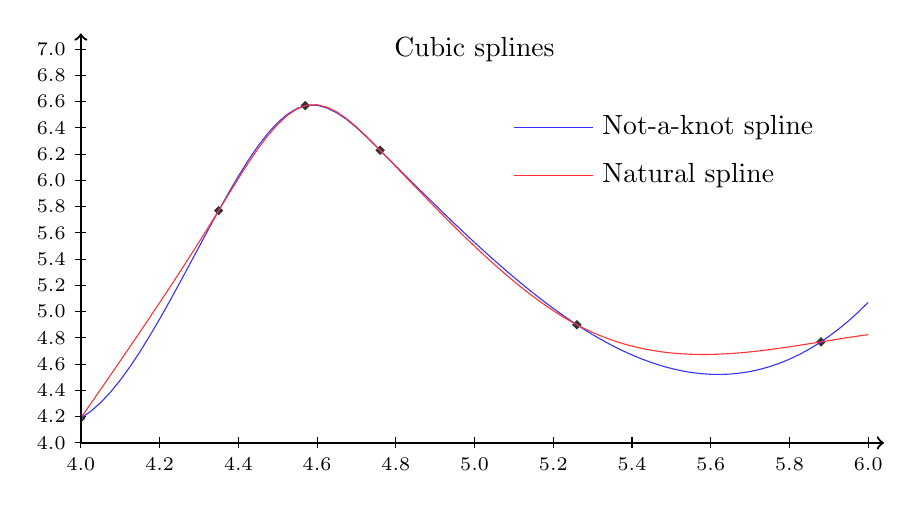
\begin{tikzpicture}
\draw (0.0,0cm + 2pt) -- (0.0, 0cm -2pt) node[below] {\scriptsize{\num[round-mode=places,round-precision=1]{4.0}}};
\draw (0.99999905,0cm + 2pt) -- (0.99999905, 0cm -2pt) node[below] {\scriptsize{\num[round-mode=places,round-precision=1]{4.2}}};
\draw (2.0000005,0cm + 2pt) -- (2.0000005, 0cm -2pt) node[below] {\scriptsize{\num[round-mode=places,round-precision=1]{4.4}}};
\draw (2.9999995,0cm + 2pt) -- (2.9999995, 0cm -2pt) node[below] {\scriptsize{\num[round-mode=places,round-precision=1]{4.6}}};
\draw (4.000001,0cm + 2pt) -- (4.000001, 0cm -2pt) node[below] {\scriptsize{\num[round-mode=places,round-precision=1]{4.8}}};
\draw (5.0,0cm + 2pt) -- (5.0, 0cm -2pt) node[below] {\scriptsize{\num[round-mode=places,round-precision=1]{5.0}}};
\draw (5.999999,0cm + 2pt) -- (5.999999, 0cm -2pt) node[below] {\scriptsize{\num[round-mode=places,round-precision=1]{5.2}}};
\draw (7.0000005,0cm + 2pt) -- (7.0000005, 0cm -2pt) node[below] {\scriptsize{\num[round-mode=places,round-precision=1]{5.4}}};
\draw (7.9999995,0cm + 2pt) -- (7.9999995, 0cm -2pt) node[below] {\scriptsize{\num[round-mode=places,round-precision=1]{5.6}}};
\draw (9.000001,0cm + 2pt) -- (9.000001, 0cm -2pt) node[below] {\scriptsize{\num[round-mode=places,round-precision=1]{5.8}}};
\draw (10.0,0cm + 2pt) -- (10.0, 0cm -2pt) node[below] {\scriptsize{\num[round-mode=places,round-precision=1]{6.0}}};
\draw (0cm + 2pt,0.    ) -- (0cm-2pt,0.    ) node[left] {\scriptsize{\num[round-mode=places,round-precision=1]{4.0}}};
\draw (0cm + 2pt,0.33333302    ) -- (0cm-2pt,0.33333302    ) node[left] {\scriptsize{\num[round-mode=places,round-precision=1]{4.2}}};
\draw (0cm + 2pt,0.6666668    ) -- (0cm-2pt,0.6666668    ) node[left] {\scriptsize{\num[round-mode=places,round-precision=1]{4.4}}};
\draw (0cm + 2pt,0.9999998    ) -- (0cm-2pt,0.9999998    ) node[left] {\scriptsize{\num[round-mode=places,round-precision=1]{4.6}}};
\draw (0cm + 2pt,1.3333336    ) -- (0cm-2pt,1.3333336    ) node[left] {\scriptsize{\num[round-mode=places,round-precision=1]{4.8}}};
\draw (0cm + 2pt,1.6666666    ) -- (0cm-2pt,1.6666666    ) node[left] {\scriptsize{\num[round-mode=places,round-precision=1]{5.0}}};
\draw (0cm + 2pt,1.9999996    ) -- (0cm-2pt,1.9999996    ) node[left] {\scriptsize{\num[round-mode=places,round-precision=1]{5.2}}};
\draw (0cm + 2pt,2.3333335    ) -- (0cm-2pt,2.3333335    ) node[left] {\scriptsize{\num[round-mode=places,round-precision=1]{5.4}}};
\draw (0cm + 2pt,2.6666665    ) -- (0cm-2pt,2.6666665    ) node[left] {\scriptsize{\num[round-mode=places,round-precision=1]{5.6}}};
\draw (0cm + 2pt,3.0000002    ) -- (0cm-2pt,3.0000002    ) node[left] {\scriptsize{\num[round-mode=places,round-precision=1]{5.8}}};
\draw (0cm + 2pt,3.3333333    ) -- (0cm-2pt,3.3333333    ) node[left] {\scriptsize{\num[round-mode=places,round-precision=1]{6.0}}};
\draw (0cm + 2pt,3.6666663    ) -- (0cm-2pt,3.6666663    ) node[left] {\scriptsize{\num[round-mode=places,round-precision=1]{6.2}}};
\draw (0cm + 2pt,4.    ) -- (0cm-2pt,4.    ) node[left] {\scriptsize{\num[round-mode=places,round-precision=1]{6.4}}};
\draw (0cm + 2pt,4.333334    ) -- (0cm-2pt,4.333334    ) node[left] {\scriptsize{\num[round-mode=places,round-precision=1]{6.6000004}}};
\draw (0cm + 2pt,4.666667    ) -- (0cm-2pt,4.666667    ) node[left] {\scriptsize{\num[round-mode=places,round-precision=1]{6.8}}};
\draw (0cm + 2pt,5.    ) -- (0cm-2pt,5.    ) node[left] {\scriptsize{\num[round-mode=places,round-precision=1]{7.0}}};
\node[] at (5.0,5.0) {Cubic splines};
\begin{scope}[]
\clip (0,0) rectangle (10,5);
\node at (0.0,0.316666654083465) [draw=black!80,fill=black!80,diamond,inner sep=0pt,minimum width =3pt,minimum height=3pt] {}; 
\node at (1.7499999739229666,2.949999882777536) [draw=black!80,fill=black!80,diamond,inner sep=0pt,minimum width =3pt,minimum height=3pt] {}; 
\node at (2.8499999575316926,4.283333163128966) [draw=black!80,fill=black!80,diamond,inner sep=0pt,minimum width =3pt,minimum height=3pt] {}; 
\node at (3.799999943375587,3.716666518979609) [draw=black!80,fill=black!80,diamond,inner sep=0pt,minimum width =3pt,minimum height=3pt] {}; 
\node at (6.299999906122685,1.4999999403953581) [draw=black!80,fill=black!80,diamond,inner sep=0pt,minimum width =3pt,minimum height=3pt] {}; 
\node at (9.399999859929085,1.2833332823382497) [draw=black!80,fill=black!80,diamond,inner sep=0pt,minimum width =3pt,minimum height=3pt] {}; 
\begin{scope}[blue!80]
\draw[] (-2.4999999627470975,7.7943914926862305) -- (-2.374999964609743,6.85271188831033);
\draw[] (-2.374999964609743,6.85271188831033) -- (-2.2499999664723886,5.985369091033453);
\draw[] (-2.2499999664723886,5.985369091033453) -- (-2.124999968335032,5.189934920066197);
\draw[] (-2.124999968335032,5.189934920066197) -- (-1.9999999701976776,4.4639811946192065);
\draw[] (-1.9999999701976776,4.4639811946192065) -- (-1.8749999720603232,3.8050797339030833);
\draw[] (-1.8749999720603232,3.8050797339030833) -- (-1.7499999739229688,3.2108023571284394);
\draw[] (-1.7499999739229688,3.2108023571284394) -- (-1.6249999757856144,2.6787208835058913);
\draw[] (-1.6249999757856144,2.6787208835058913) -- (-1.4999999776482578,2.206407132246049);
\draw[] (-1.4999999776482578,2.206407132246049) -- (-1.3749999795109031,1.7914329225595402);
\draw[] (-1.3749999795109031,1.7914329225595402) -- (-1.2499999813735487,1.431370073656974);
\draw[] (-1.2499999813735487,1.431370073656974) -- (-1.1249999832361943,1.1237904047489642);
\draw[] (-1.1249999832361943,1.1237904047489642) -- (-0.9999999850988399,0.8662657350461275);
\draw[] (-0.9999999850988399,0.8662657350461275) -- (-0.8749999869614833,0.6563678837590736);
\draw[] (-0.8749999869614833,0.6563678837590736) -- (-0.7499999888241289,0.49166867009842874);
\draw[] (-0.7499999888241289,0.49166867009842874) -- (-0.6249999906867744,0.36973991327480216);
\draw[] (-0.6249999906867744,0.36973991327480216) -- (-0.49999999254941996,0.2881534324988066);
\draw[] (-0.49999999254941996,0.2881534324988066) -- (-0.3749999944120655,0.24448104698106043);
\draw[] (-0.3749999944120655,0.24448104698106043) -- (-0.24999999627470887,0.23629457593217776);
\draw[] (-0.24999999627470887,0.23629457593217776) -- (-0.12499999813735443,0.26116583856277414);
\draw[] (-0.12499999813735443,0.26116583856277414) -- (0.0,0.316666654083465);
\draw[] (0.0,0.316666654083465) -- (0.12499999813735665,0.4003688417048675);
\draw[] (0.12499999813735665,0.4003688417048675) -- (0.24999999627470887,0.5098442206375896);
\draw[] (0.24999999627470887,0.5098442206375896) -- (0.3749999944120655,0.6426646100922557);
\draw[] (0.3749999944120655,0.6426646100922557) -- (0.49999999254941774,0.7964018292794712);
\draw[] (0.49999999254941774,0.7964018292794712) -- (0.6249999906867744,0.9686276974098632);
\draw[] (0.6249999906867744,0.9686276974098632) -- (0.749999988824131,1.1569140336940429);
\draw[] (0.749999988824131,1.1569140336940429) -- (0.8749999869614833,1.358832657342614);
\draw[] (0.8749999869614833,1.358832657342614) -- (0.9999999850988399,1.5719553875662082);
\draw[] (0.9999999850988399,1.5719553875662082) -- (1.124999983236192,1.793854043575428);
\draw[] (1.124999983236192,1.793854043575428) -- (1.2499999813735487,2.0221004445808974);
\draw[] (1.2499999813735487,2.0221004445808974) -- (1.3749999795109054,2.2542664097932303);
\draw[] (1.3749999795109054,2.2542664097932303) -- (1.4999999776482578,2.487923758423034);
\draw[] (1.4999999776482578,2.487923758423034) -- (1.6249999757856144,2.7206443096809374);
\draw[] (1.6249999757856144,2.7206443096809374) -- (1.7499999739229666,2.9499998827775373);
\draw[] (1.7499999739229666,2.9499998827775373) -- (1.8749999720603232,3.1733231579063315);
\draw[] (1.8749999720603232,3.1733231579063315) -- (1.9999999701976798,3.386990259192244);
\draw[] (1.9999999701976798,3.386990259192244) -- (2.124999968335032,3.5871381717430655);
\draw[] (2.124999968335032,3.5871381717430655) -- (2.2499999664723886,3.7699038806666065);
\draw[] (2.2499999664723886,3.7699038806666065) -- (2.374999964609741,3.931424371070651);
\draw[] (2.374999964609741,3.931424371070651) -- (2.4999999627470975,4.06783662806301);
\draw[] (2.4999999627470975,4.06783662806301) -- (2.624999960884454,4.17527763675147);
\draw[] (2.624999960884454,4.17527763675147) -- (2.7499999590218063,4.24988438224383);
\draw[] (2.7499999590218063,4.24988438224383) -- (2.874999957159163,4.287805970399012);
\draw[] (2.874999957159163,4.287805970399012) -- (2.9999999552965155,4.287761106314666);
\draw[] (2.9999999552965155,4.287761106314666) -- (3.124999953433872,4.254201610371051);
\draw[] (3.124999953433872,4.254201610371051) -- (3.249999951571229,4.192355031020499);
\draw[] (3.249999951571229,4.192355031020499) -- (3.374999949708581,4.1074489167153505);
\draw[] (3.374999949708581,4.1074489167153505) -- (3.4999999478459376,4.004710815907926);
\draw[] (3.4999999478459376,4.004710815907926) -- (3.62499994598329,3.88936827705057);
\draw[] (3.62499994598329,3.88936827705057) -- (3.7499999441206464,3.766648848595603);
\draw[] (3.7499999441206464,3.766648848595603) -- (3.874999942258003,3.641599909911412);
\draw[] (3.874999942258003,3.641599909911412) -- (3.9999999403953552,3.5165729770361955);
\draw[] (3.9999999403953552,3.5165729770361955) -- (4.124999938532712,3.3918442850782133);
\draw[] (4.124999938532712,3.3918442850782133) -- (4.249999936670064,3.2676366857134576);
\draw[] (4.249999936670064,3.2676366857134576) -- (4.374999934807421,3.144173030617912);
\draw[] (4.374999934807421,3.144173030617912) -- (4.499999932944777,3.021676171467562);
\draw[] (4.499999932944777,3.021676171467562) -- (4.6249999310821295,2.9003689599384015);
\draw[] (4.6249999310821295,2.9003689599384015) -- (4.749999929219486,2.7804742477064077);
\draw[] (4.749999929219486,2.7804742477064077) -- (4.874999927356838,2.6622148864475754);
\draw[] (4.874999927356838,2.6622148864475754) -- (4.999999925494195,2.545813727837884);
\draw[] (4.999999925494195,2.545813727837884) -- (5.1249999236315515,2.4314936235533224);
\draw[] (5.1249999236315515,2.4314936235533224) -- (5.249999921768904,2.3194774252698838);
\draw[] (5.249999921768904,2.3194774252698838) -- (5.37499991990626,2.2099879846635475);
\draw[] (5.37499991990626,2.2099879846635475) -- (5.4999999180436125,2.103248153410304);
\draw[] (5.4999999180436125,2.103248153410304) -- (5.624999916180969,1.9994807831861359);
\draw[] (5.624999916180969,1.9994807831861359) -- (5.749999914318326,1.8989087256670316);
\draw[] (5.749999914318326,1.8989087256670316) -- (5.874999912455678,1.8017548325289818);
\draw[] (5.874999912455678,1.8017548325289818) -- (5.999999910593035,1.708241955447969);
\draw[] (5.999999910593035,1.708241955447969) -- (6.124999908730388,1.6185929460999828);
\draw[] (6.124999908730388,1.6185929460999828) -- (6.249999906867744,1.533030656161004);
\draw[] (6.249999906867744,1.533030656161004) -- (6.374999905005101,1.451776384534055);
\draw[] (6.374999905005101,1.451776384534055) -- (6.499999903142453,1.3750281960377477);
\draw[] (6.499999903142453,1.3750281960377477) -- (6.62499990127981,1.3029662698464899);
\draw[] (6.62499990127981,1.3029662698464899) -- (6.749999899417162,1.2357703250538243);
\draw[] (6.749999899417162,1.2357703250538243) -- (6.874999897554519,1.173620080753285);
\draw[] (6.874999897554519,1.173620080753285) -- (6.999999895691875,1.116695256038412);
\draw[] (6.999999895691875,1.116695256038412) -- (7.124999893829227,1.0651755700027439);
\draw[] (7.124999893829227,1.0651755700027439) -- (7.249999891966584,1.0192407417398162);
\draw[] (7.249999891966584,1.0192407417398162) -- (7.374999890103936,0.9790704903431704);
\draw[] (7.374999890103936,0.9790704903431704) -- (7.499999888241293,0.944844534906336);
\draw[] (7.499999888241293,0.944844534906336) -- (7.6249998863786494,0.9167425945228603);
\draw[] (7.6249998863786494,0.9167425945228603) -- (7.749999884516006,0.8949443882862762);
\draw[] (7.749999884516006,0.8949443882862762) -- (7.874999882653358,0.879629635290119);
\draw[] (7.874999882653358,0.879629635290119) -- (7.9999998807907104,0.8709780546279331);
\draw[] (7.9999998807907104,0.8709780546279331) -- (8.124999878928067,0.8691693653932512);
\draw[] (8.124999878928067,0.8691693653932512) -- (8.249999877065424,0.8743832866796089);
\draw[] (8.249999877065424,0.8743832866796089) -- (8.37499987520278,0.8867995375805503);
\draw[] (8.37499987520278,0.8867995375805503) -- (8.499999873340133,0.9065978371896083);
\draw[] (8.499999873340133,0.9065978371896083) -- (8.624999871477485,0.9339579046003212);
\draw[] (8.624999871477485,0.9339579046003212) -- (8.749999869614841,0.9690594589062291);
\draw[] (8.749999869614841,0.9690594589062291) -- (8.874999867752198,1.0120822192008692);
\draw[] (8.874999867752198,1.0120822192008692) -- (8.999999865889555,1.0632059045777764);
\draw[] (8.999999865889555,1.0632059045777764) -- (9.124999864026908,1.12261023413049);
\draw[] (9.124999864026908,1.12261023413049) -- (9.249999862164259,1.190474926952545);
\draw[] (9.249999862164259,1.190474926952545) -- (9.374999860301616,1.2669797021374845);
\draw[] (9.374999860301616,1.2669797021374845) -- (9.499999858438972,1.3523042787788442);
\draw[] (9.499999858438972,1.3523042787788442) -- (9.624999856576329,1.4466283759701621);
\draw[] (9.624999856576329,1.4466283759701621) -- (9.749999854713682,1.5501317128049699);
\draw[] (9.749999854713682,1.5501317128049699) -- (9.874999852851033,1.6629940083768073);
\draw[] (9.874999852851033,1.6629940083768073) -- (9.99999985098839,1.7853949817792232);
\end{scope}
\begin{scope}[red!80]
\draw[] (-2.4999999627470975,-3.605941027545164) -- (-2.374999964609743,-3.38062413015895);
\draw[] (-2.374999964609743,-3.38062413015895) -- (-2.2499999664723886,-3.159797465588856);
\draw[] (-2.2499999664723886,-3.159797465588856) -- (-2.124999968335032,-2.943224705791926);
\draw[] (-2.124999968335032,-2.943224705791926) -- (-1.9999999701976776,-2.730669522725212);
\draw[] (-1.9999999701976776,-2.730669522725212) -- (-1.8749999720603232,-2.5218955883457586);
\draw[] (-1.8749999720603232,-2.5218955883457586) -- (-1.7499999739229688,-2.3166665746106103);
\draw[] (-1.7499999739229688,-2.3166665746106103) -- (-1.6249999757856144,-2.114746153476813);
\draw[] (-1.6249999757856144,-2.114746153476813) -- (-1.4999999776482578,-1.9158979969014112);
\draw[] (-1.4999999776482578,-1.9158979969014112) -- (-1.3749999795109031,-1.7198857768414577);
\draw[] (-1.3749999795109031,-1.7198857768414577) -- (-1.2499999813735487,-1.526473165253995);
\draw[] (-1.2499999813735487,-1.526473165253995) -- (-1.1249999832361943,-1.3354238340960685);
\draw[] (-1.1249999832361943,-1.3354238340960685) -- (-0.9999999850988399,-1.1465014553247257);
\draw[] (-0.9999999850988399,-1.1465014553247257) -- (-0.8749999869614833,-0.95946970089701);
\draw[] (-0.8749999869614833,-0.95946970089701) -- (-0.7499999888241289,-0.7740922427699727);
\draw[] (-0.7499999888241289,-0.7740922427699727) -- (-0.6249999906867744,-0.5901327529006577);
\draw[] (-0.6249999906867744,-0.5901327529006577) -- (-0.49999999254941996,-0.4073549032461111);
\draw[] (-0.49999999254941996,-0.4073549032461111) -- (-0.3749999944120655,-0.2255223657633807);
\draw[] (-0.3749999944120655,-0.2255223657633807) -- (-0.24999999627470887,-0.04439881240950658);
\draw[] (-0.24999999627470887,-0.04439881240950658) -- (-0.12499999813735443,0.1362520848584554);
\draw[] (-0.12499999813735443,0.1362520848584554) -- (0.0,0.316666654083465);
\draw[] (0.0,0.316666654083465) -- (0.12499999813735665,0.4970812233084776);
\draw[] (0.12499999813735665,0.4970812233084776) -- (0.24999999627470887,0.677732120576436);
\draw[] (0.24999999627470887,0.677732120576436) -- (0.3749999944120655,0.8588556739303093);
\draw[] (0.3749999944120655,0.8588556739303093) -- (0.49999999254941774,1.040688211413039);
\draw[] (0.49999999254941774,1.040688211413039) -- (0.6249999906867744,1.2234660610675885);
\draw[] (0.6249999906867744,1.2234660610675885) -- (0.749999988824131,1.4074255509369065);
\draw[] (0.749999988824131,1.4074255509369065) -- (0.8749999869614833,1.5928030090639387);
\draw[] (0.8749999869614833,1.5928030090639387) -- (0.9999999850988399,1.7798347634916558);
\draw[] (0.9999999850988399,1.7798347634916558) -- (1.124999983236192,1.9687571422629948);
\draw[] (1.124999983236192,1.9687571422629948) -- (1.2499999813735487,2.159806473420925);
\draw[] (1.2499999813735487,2.159806473420925) -- (1.3749999795109054,2.353219085008392);
\draw[] (1.3749999795109054,2.353219085008392) -- (1.4999999776482578,2.5492313050683406);
\draw[] (1.4999999776482578,2.5492313050683406) -- (1.6249999757856144,2.748079461643744);
\draw[] (1.6249999757856144,2.748079461643744) -- (1.7499999739229666,2.9499998827775373);
\draw[] (1.7499999739229666,2.9499998827775373) -- (1.8749999720603232,3.154329772046608);
\draw[] (1.8749999720603232,3.154329772046608) -- (1.9999999701976798,3.356809835163513);
\draw[] (1.9999999701976798,3.356809835163513) -- (2.124999968335032,3.552281653374717);
\draw[] (2.124999968335032,3.552281653374717) -- (2.2499999664723886,3.735586807926718);
\draw[] (2.2499999664723886,3.735586807926718) -- (2.374999964609741,3.9015668800659786);
\draw[] (2.374999964609741,3.9015668800659786) -- (2.4999999627470975,4.045063451038991);
\draw[] (2.4999999627470975,4.045063451038991) -- (2.624999960884454,4.160918102092223);
\draw[] (2.624999960884454,4.160918102092223) -- (2.7499999590218063,4.243972414472157);
\draw[] (2.7499999590218063,4.243972414472157) -- (2.874999957159163,4.289082111375187);
\draw[] (2.874999957159163,4.289082111375187) -- (2.9999999552965155,4.294101009379233);
\draw[] (2.9999999552965155,4.294101009379233) -- (3.124999953433872,4.263572067371012);
\draw[] (3.124999953433872,4.263572067371012) -- (3.249999951571229,4.202943329031665);
\draw[] (3.249999951571229,4.202943329031665) -- (3.374999949708581,4.117662838042336);
\draw[] (3.374999949708581,4.117662838042336) -- (3.4999999478459376,4.01317863808416);
\draw[] (3.4999999478459376,4.01317863808416) -- (3.62499994598329,3.8949387728382847);
\draw[] (3.62499994598329,3.8949387728382847) -- (3.7499999441206464,3.768391285985844);
\draw[] (3.7499999441206464,3.768391285985844) -- (3.874999942258003,3.6388018959505035);
\draw[] (3.874999942258003,3.6388018959505035) -- (3.9999999403953552,3.5087081950810326);
\draw[] (3.9999999403953552,3.5087081950810326) -- (4.124999938532712,3.3785476588715095);
\draw[] (4.124999938532712,3.3785476588715095) -- (4.249999936670064,3.248703740517511);
\draw[] (4.249999936670064,3.248703740517511) -- (4.374999934807421,3.1195598932146047);
\draw[] (4.374999934807421,3.1195598932146047) -- (4.499999932944777,2.9914995701583624);
\draw[] (4.499999932944777,2.9914995701583624) -- (4.6249999310821295,2.864906224544363);
\draw[] (4.6249999310821295,2.864906224544363) -- (4.749999929219486,2.740163309568167);
\draw[] (4.749999929219486,2.740163309568167) -- (4.874999927356838,2.617654278425355);
\draw[] (4.874999927356838,2.617654278425355) -- (4.999999925494195,2.497762584311492);
\draw[] (4.999999925494195,2.497762584311492) -- (5.1249999236315515,2.380871680422152);
\draw[] (5.1249999236315515,2.380871680422152) -- (5.249999921768904,2.267365019952912);
\draw[] (5.249999921768904,2.267365019952912) -- (5.37499991990626,2.157626056099335);
\draw[] (5.37499991990626,2.157626056099335) -- (5.4999999180436125,2.0520382420570016);
\draw[] (5.4999999180436125,2.0520382420570016) -- (5.624999916180969,1.9509850310214718);
\draw[] (5.624999916180969,1.9509850310214718) -- (5.749999914318326,1.8548498761883265);
\draw[] (5.749999914318326,1.8548498761883265) -- (5.874999912455678,1.764016230753138);
\draw[] (5.874999912455678,1.764016230753138) -- (5.999999910593035,1.6788675479114719);
\draw[] (5.999999910593035,1.6788675479114719) -- (6.124999908730388,1.5997872808589044);
\draw[] (6.124999908730388,1.5997872808589044) -- (6.249999906867744,1.5271588827910019);
\draw[] (6.249999906867744,1.5271588827910019) -- (6.374999905005101,1.4613418576961836);
\draw[] (6.374999905005101,1.4613418576961836) -- (6.499999903142453,1.4023373584631706);
\draw[] (6.499999903142453,1.4023373584631706) -- (6.62499990127981,1.3498706785945276);
\draw[] (6.62499990127981,1.3498706785945276) -- (6.749999899417162,1.3036600155314544);
\draw[] (6.749999899417162,1.3036600155314544) -- (6.874999897554519,1.2634235667151321);
\draw[] (6.874999897554519,1.2634235667151321) -- (6.999999895691875,1.2288795295867583);
\draw[] (6.999999895691875,1.2288795295867583) -- (7.124999893829227,1.1997461015875226);
\draw[] (7.124999893829227,1.1997461015875226) -- (7.249999891966584,1.175741480158612);
\draw[] (7.249999891966584,1.175741480158612) -- (7.374999890103936,1.1565838627412233);
\draw[] (7.374999890103936,1.1565838627412233) -- (7.499999888241293,1.1419914467765409);
\draw[] (7.499999888241293,1.1419914467765409) -- (7.6249998863786494,1.1316824297057606);
\draw[] (7.6249998863786494,1.1316824297057606) -- (7.749999884516006,1.1253750089700705);
\draw[] (7.749999884516006,1.1253750089700705) -- (7.874999882653358,1.1227873820106633);
\draw[] (7.874999882653358,1.1227873820106633) -- (7.9999998807907104,1.1236377462687277);
\draw[] (7.9999998807907104,1.1236377462687277) -- (8.124999878928067,1.127644299185455);
\draw[] (8.124999878928067,1.127644299185455) -- (8.249999877065424,1.1345252382020363);
\draw[] (8.249999877065424,1.1345252382020363) -- (8.37499987520278,1.143998760759663);
\draw[] (8.37499987520278,1.143998760759663) -- (8.499999873340133,1.155783064299525);
\draw[] (8.499999873340133,1.155783064299525) -- (8.624999871477485,1.1695963462628136);
\draw[] (8.624999871477485,1.1695963462628136) -- (8.749999869614841,1.1851568040907217);
\draw[] (8.749999869614841,1.1851568040907217) -- (8.874999867752198,1.2021826352244345);
\draw[] (8.874999867752198,1.2021826352244345) -- (8.999999865889555,1.220392037105148);
\draw[] (8.999999865889555,1.220392037105148) -- (9.124999864026908,1.2395032071740488);
\draw[] (9.124999864026908,1.2395032071740488) -- (9.249999862164259,1.2592343428723314);
\draw[] (9.249999862164259,1.2592343428723314) -- (9.374999860301616,1.2793036416411872);
\draw[] (9.374999860301616,1.2793036416411872) -- (9.499999858438972,1.2994293009218014);
\draw[] (9.499999858438972,1.2994293009218014) -- (9.624999856576329,1.3193295181553697);
\draw[] (9.624999856576329,1.3193295181553697) -- (9.749999854713682,1.3387224907830808);
\draw[] (9.749999854713682,1.3387224907830808) -- (9.874999852851033,1.3573264162461258);
\draw[] (9.874999852851033,1.3573264162461258) -- (9.99999985098839,1.3748594919856976);
\end{scope}
\end{scope}
\draw[blue!80] (5.5,4.0) -- (6.5,4.0);
\node[right,] at (6.5,4.0) {Not-a-knot spline};
\draw[red!80] (5.5,3.4) -- (6.5,3.4);
\node[right,] at (6.5,3.4) {Natural spline};
\draw[thick,->] (0.0,0.0) -- (10.2,0.0);
\draw[thick,->] (0.0,0.0) -- (0.0,5.2);
\end{tikzpicture}
%%% Local Variables: 
%%% mode: latex 
%%% TeX-master: "master" 
%%% End:


\captionsetup{singlelinecheck=off}
\caption[asdf]{Cubic splines, with different end point conditions.}
\end{figure}
\section{Sub figures}
\begin{figure}[H]
\centering
%%% AUTO GENERATED CODE
\documentclass{standalone}
\ifx\HCode\UnDef\else\def\pgfsysdriver{pgfsys-tex4ht.def}\fi
\usepackage[usenames,dvipsnames,svgnames,table]{xcolor}
\usepackage{tikz}
\usepackage{color}
\usepackage{siunitx}
\usetikzlibrary{arrows,shapes}
\begin{document}
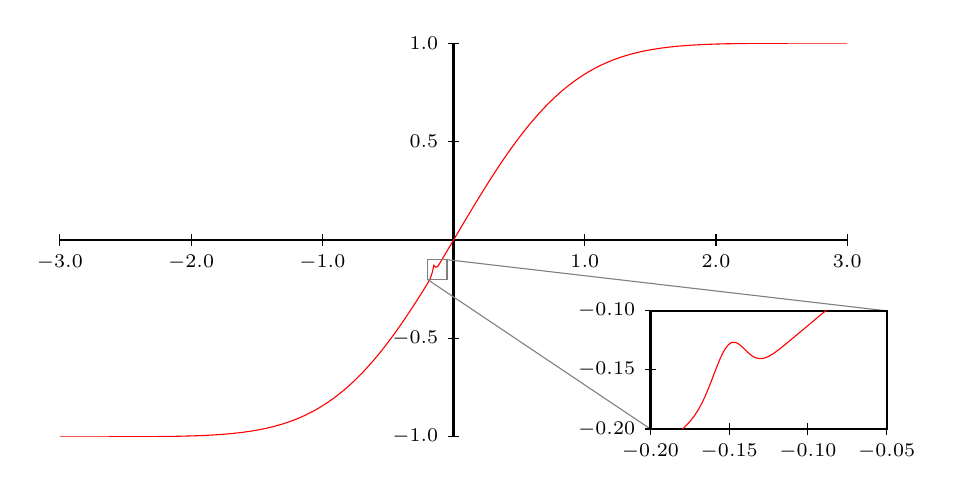
\begin{tikzpicture}[]
\begin{scope}[shift={(0.0,0.0)}]
\pgfsetxvec{\pgfpoint{1.6666666666666667cm}{0cm}}
\pgfsetyvec{\pgfpoint{0cm}{2.5cm}}
\begin{scope}[shift={(3.0,1.0)}]
\begin{scope}[thick,black,fill=white]
\pgfpathmoveto{ \pgfpointxy {-3.0} {0.0}}
\pgfpathlineto{ \pgfpointxy {3.0} {0.0}}
\pgfpathmoveto{ \pgfpointxy {0.0} {-1.0}}
\pgfpathlineto{ \pgfpointxy {0.0} {1.0}}
\pgfusepath{ stroke, }
\end{scope}
\begin{scope}[yshift=2.5cm]
\draw[] [shift={(-3.0,-1.0)}] (0,2pt) -- (0,-2pt) node[below]{ \scriptsize{\num[round-mode=places,round-precision=1]{-3.0}}};
\draw[] [shift={(-2.0,-1.0)}] (0,2pt) -- (0,-2pt) node[below]{ \scriptsize{\num[round-mode=places,round-precision=1]{-2.0}}};
\draw[] [shift={(-1.0,-1.0)}] (0,2pt) -- (0,-2pt) node[below]{ \scriptsize{\num[round-mode=places,round-precision=1]{-1.0}}};
\draw[] [shift={(1.0,-1.0)}] (0,2pt) -- (0,-2pt) node[below]{ \scriptsize{\num[round-mode=places,round-precision=1]{1.0}}};
\draw[] [shift={(2.0,-1.0)}] (0,2pt) -- (0,-2pt) node[below]{ \scriptsize{\num[round-mode=places,round-precision=1]{2.0}}};
\draw[] [shift={(3.0,-1.0)}] (0,2pt) -- (0,-2pt) node[below]{ \scriptsize{\num[round-mode=places,round-precision=1]{3.0}}};
\end{scope}
\begin{scope}[xshift=5.0cm]
\draw[] [shift={(-3.0,-1.0)}] (2pt,0) -- (-2pt,0) node[left]{ \scriptsize{\num[round-mode=places,round-precision=1]{-1.0}}};
\draw[] [shift={(-3.0,-0.5)}] (2pt,0) -- (-2pt,0) node[left]{ \scriptsize{\num[round-mode=places,round-precision=1]{-0.5}}};
\draw[] [shift={(-3.0,0.5)}] (2pt,0) -- (-2pt,0) node[left]{ \scriptsize{\num[round-mode=places,round-precision=1]{0.5}}};
\draw[] [shift={(-3.0,1.0)}] (2pt,0) -- (-2pt,0) node[left]{ \scriptsize{\num[round-mode=places,round-precision=1]{1.0}}};
\end{scope}
\end{scope}
\pgfsetxvec{\pgfpoint{1cm}{0cm}}
\pgfsetyvec{\pgfpoint{0cm}{1cm}}
\end{scope}
\begin{scope}[]
\pgfpathmoveto{ \pgfpointadd{\pgfpointxy {0.0} {0.0}} {\pgfpoint{0cm}{0cm}} }
\pgfpathlineto{ \pgfpointadd{\pgfpointxy {0.0} {0.0}} {\pgfpoint{10cm}{0cm}} }
\pgfpathlineto{ \pgfpointadd{\pgfpointxy {0.0} {0.0}} {\pgfpoint{10cm}{5cm}} }
\pgfpathlineto{ \pgfpointadd{\pgfpointxy {0.0} {0.0}} {\pgfpoint{0cm}{5cm}} }
\pgfpathclose
\pgfusepath{  clip, }
\begin{scope}[shift={(0.0,0.0)}]
\pgfsetxvec{\pgfpoint{1.6666666666666667cm}{0cm}}
\pgfsetyvec{\pgfpoint{0cm}{2.5cm}}
\begin{scope}[shift={(3.0,1.0)}]
\begin{scope}[red]
\pgfpathmoveto{ \pgfpointxy {-3.0} {-0.9999778948503159}}
\pgfpathlineto{ \pgfpointxy {-2.985} {-0.9999757083515112}}
\pgfpathlineto{ \pgfpointxy {-2.97} {-0.9999733170632894}}
\pgfpathlineto{ \pgfpointxy {-2.955} {-0.999970702980543}}
\pgfpathlineto{ \pgfpointxy {-2.94} {-0.9999678466302895}}
\pgfpathlineto{ \pgfpointxy {-2.925} {-0.9999647269627512}}
\pgfpathlineto{ \pgfpointxy {-2.91} {-0.9999613212353085}}
\pgfpathlineto{ \pgfpointxy {-2.895} {-0.9999576048889374}}
\pgfpathlineto{ \pgfpointxy {-2.88} {-0.9999535514167339}}
\pgfpathlineto{ \pgfpointxy {-2.865} {-0.9999491322241092}}
\pgfpathlineto{ \pgfpointxy {-2.85} {-0.9999443164802247}}
\pgfpathlineto{ \pgfpointxy {-2.835} {-0.9999390709602284}}
\pgfpathlineto{ \pgfpointxy {-2.82} {-0.9999333598778289}}
\pgfpathlineto{ \pgfpointxy {-2.805} {-0.9999271447077411}}
\pgfpathlineto{ \pgfpointxy {-2.79} {-0.9999203839975161}}
\pgfpathlineto{ \pgfpointxy {-2.775} {-0.9999130331682573}}
\pgfpathlineto{ \pgfpointxy {-2.76} {-0.9999050443037141}}
\pgfpathlineto{ \pgfpointxy {-2.745} {-0.9998963659272275}}
\pgfpathlineto{ \pgfpointxy {-2.73} {-0.9998869427659972}}
\pgfpathlineto{ \pgfpointxy {-2.715} {-0.9998767155021218}}
\pgfpathlineto{ \pgfpointxy {-2.7} {-0.9998656205098599}}
\pgfpathlineto{ \pgfpointxy {-2.685} {-0.9998535895785484}}
\pgfpathlineto{ \pgfpointxy {-2.67} {-0.9998405496206055}}
\pgfpathlineto{ \pgfpointxy {-2.6550000000000002} {-0.9998264223640424}}
\pgfpathlineto{ \pgfpointxy {-2.64} {-0.9998111240288999}}
\pgfpathlineto{ \pgfpointxy {-2.625} {-0.9997945649870237}}
\pgfpathlineto{ \pgfpointxy {-2.61} {-0.9997766494045888}}
\pgfpathlineto{ \pgfpointxy {-2.595} {-0.9997572748667864}}
\pgfpathlineto{ \pgfpointxy {-2.58} {-0.999736331984083}}
\pgfpathlineto{ \pgfpointxy {-2.565} {-0.9997137039794691}}
\pgfpathlineto{ \pgfpointxy {-2.55} {-0.9996892662561212}}
\pgfpathlineto{ \pgfpointxy {-2.535} {-0.9996628859449036}}
\pgfpathlineto{ \pgfpointxy {-2.52} {-0.9996344214311546}}
\pgfpathlineto{ \pgfpointxy {-2.505} {-0.9996037218602093}}
\pgfpathlineto{ \pgfpointxy {-2.49} {-0.9995706266211303}}
\pgfpathlineto{ \pgfpointxy {-2.475} {-0.9995349648081364}}
\pgfpathlineto{ \pgfpointxy {-2.46} {-0.9994965546592407}}
\pgfpathlineto{ \pgfpointxy {-2.4450000000000003} {-0.9994552029716378}}
\pgfpathlineto{ \pgfpointxy {-2.43} {-0.9994107044934063}}
\pgfpathlineto{ \pgfpointxy {-2.415} {-0.9993628412911277}}
\pgfpathlineto{ \pgfpointxy {-2.4} {-0.99931138209306}}
\pgfpathlineto{ \pgfpointxy {-2.385} {-0.9992560816075419}}
\pgfpathlineto{ \pgfpointxy {-2.37} {-0.9991966798163542}}
\pgfpathlineto{ \pgfpointxy {-2.355} {-0.999132901242809}}
\pgfpathlineto{ \pgfpointxy {-2.34} {-0.9990644541943925}}
\pgfpathlineto{ \pgfpointxy {-2.325} {-0.9989910299798491}}
\pgfpathlineto{ \pgfpointxy {-2.31} {-0.9989123021006515}}
\pgfpathlineto{ \pgfpointxy {-2.295} {-0.9988279254168742}}
\pgfpathlineto{ \pgfpointxy {-2.2800000000000002} {-0.9987375352875576}}
\pgfpathlineto{ \pgfpointxy {-2.265} {-0.9986407466857308}}
\pgfpathlineto{ \pgfpointxy {-2.25} {-0.9985371532883388}}
\pgfpathlineto{ \pgfpointxy {-2.235} {-0.9984263265414133}}
\pgfpathlineto{ \pgfpointxy {-2.2199999999999998} {-0.9983078147009155}}
\pgfpathlineto{ \pgfpointxy {-2.205} {-0.9981811418497791}}
\pgfpathlineto{ \pgfpointxy {-2.19} {-0.9980458068917848}}
\pgfpathlineto{ \pgfpointxy {-2.175} {-0.9979012825230041}}
\pgfpathlineto{ \pgfpointxy {-2.16} {-0.9977470141816697}}
\pgfpathlineto{ \pgfpointxy {-2.145} {-0.997582418977438}}
\pgfpathlineto{ \pgfpointxy {-2.13} {-0.9974068846011453}}
\pgfpathlineto{ \pgfpointxy {-2.115} {-0.997219768216276}}
\pgfpathlineto{ \pgfpointxy {-2.1} {-0.9970203953335013}}
\pgfpathlineto{ \pgfpointxy {-2.085} {-0.9968080586697832}}
\pgfpathlineto{ \pgfpointxy {-2.0700000000000003} {-0.9965820169936752}}
\pgfpathlineto{ \pgfpointxy {-2.055} {-0.9963414939586048}}
\pgfpathlineto{ \pgfpointxy {-2.04} {-0.9960856769260644}}
\pgfpathlineto{ \pgfpointxy {-2.025} {-0.9958137157807956}}
\pgfpathlineto{ \pgfpointxy {-2.01} {-0.9955247217402033}}
\pgfpathlineto{ \pgfpointxy {-1.995} {-0.9952177661603995}}
\pgfpathlineto{ \pgfpointxy {-1.98} {-0.9948918793414291}}
\pgfpathlineto{ \pgfpointxy {-1.965} {-0.9945460493344039}}
\pgfpathlineto{ \pgfpointxy {-1.95} {-0.9941792207534235}}
\pgfpathlineto{ \pgfpointxy {-1.935} {-0.9937902935953322}}
\pgfpathlineto{ \pgfpointxy {-1.92} {-0.9933781220705278}}
\pgfpathlineto{ \pgfpointxy {-1.905} {-0.992941513448194}}
\pgfpathlineto{ \pgfpointxy {-1.8900000000000001} {-0.9924792269195024}}
\pgfpathlineto{ \pgfpointxy {-1.875} {-0.9919899724824818}}
\pgfpathlineto{ \pgfpointxy {-1.86} {-0.9914724098524189}}
\pgfpathlineto{ \pgfpointxy {-1.845} {-0.9909251474018062}}
\pgfpathlineto{ \pgfpointxy {-1.83} {-0.9903467411340076}}
\pgfpathlineto{ \pgfpointxy {-1.815} {-0.9897356936949588}}
\pgfpathlineto{ \pgfpointxy {-1.8} {-0.9890904534273609}}
\pgfpathlineto{ \pgfpointxy {-1.7850000000000001} {-0.9884094134719639}}
\pgfpathlineto{ \pgfpointxy {-1.77} {-0.9876909109206615}}
\pgfpathlineto{ \pgfpointxy {-1.7550000000000001} {-0.9869332260262446}}
\pgfpathlineto{ \pgfpointxy {-1.74} {-0.9861345814737644}}
\pgfpathlineto{ \pgfpointxy {-1.725} {-0.9852931417185677}}
\pgfpathlineto{ \pgfpointxy {-1.71} {-0.9844070123961483}}
\pgfpathlineto{ \pgfpointxy {-1.695} {-0.9834742398090428}}
\pgfpathlineto{ \pgfpointxy {-1.6800000000000002} {-0.9824928104960676}}
\pgfpathlineto{ \pgfpointxy {-1.665} {-0.9814606508892384}}
\pgfpathlineto{ \pgfpointxy {-1.6500000000000001} {-0.9803756270637614}}
\pgfpathlineto{ \pgfpointxy {-1.635} {-0.9792355445865027}}
\pgfpathlineto{ \pgfpointxy {-1.62} {-0.9780381484683515}}
\pgfpathlineto{ \pgfpointxy {-1.605} {-0.9767811232258793}}
\pgfpathlineto{ \pgfpointxy {-1.59} {-0.9754620930576753}}
\pgfpathlineto{ \pgfpointxy {-1.575} {-0.9740786221406821}}
\pgfpathlineto{ \pgfpointxy {-1.56} {-0.9726282150517984}}
\pgfpathlineto{ \pgfpointxy {-1.5450000000000002} {-0.97110831731992}}
\pgfpathlineto{ \pgfpointxy {-1.53} {-0.9695163161134889}}
\pgfpathlineto{ \pgfpointxy {-1.5150000000000001} {-0.9678495410684881}}
\pgfpathlineto{ \pgfpointxy {-1.5} {-0.9661052652616654}}
\pgfpathlineto{ \pgfpointxy {-1.485} {-0.9642807063336017}}
\pgfpathlineto{ \pgfpointxy {-1.47} {-0.9623730277660346}}
\pgfpathlineto{ \pgfpointxy {-1.455} {-0.9603793403176331}}
\pgfpathlineto{ \pgfpointxy {-1.44} {-0.958296703622169}}
\pgfpathlineto{ \pgfpointxy {-1.425} {-0.9561221279527699}}
\pgfpathlineto{ \pgfpointxy {-1.4100000000000001} {-0.9538525761556357}}
\pgfpathlineto{ \pgfpointxy {-1.395} {-0.9514849657562949}}
\pgfpathlineto{ \pgfpointxy {-1.3800000000000001} {-0.9490161712411282}}
\pgfpathlineto{ \pgfpointxy {-1.365} {-0.9464430265165276}}
\pgfpathlineto{ \pgfpointxy {-1.35} {-0.943762327547669}}
\pgfpathlineto{ \pgfpointxy {-1.335} {-0.9409708351784686}}
\pgfpathlineto{ \pgfpointxy {-1.32} {-0.9380652781338571}}
\pgfpathlineto{ \pgfpointxy {-1.3050000000000002} {-0.9350423562050534}}
\pgfpathlineto{ \pgfpointxy {-1.29} {-0.9318987436180433}}
\pgfpathlineto{ \pgfpointxy {-1.2750000000000001} {-0.9286310925849711}}
\pgfpathlineto{ \pgfpointxy {-1.26} {-0.92523603703764}}
\pgfpathlineto{ \pgfpointxy {-1.245} {-0.92171019654178}}
\pgfpathlineto{ \pgfpointxy {-1.23} {-0.9180501803901957}}
\pgfpathlineto{ \pgfpointxy {-1.215} {-0.9142525918723391}}
\pgfpathlineto{ \pgfpointxy {-1.2000000000000002} {-0.910314032717273}}
\pgfpathlineto{ \pgfpointxy {-1.185} {-0.9062311077063987}}
\pgfpathlineto{ \pgfpointxy {-1.1700000000000002} {-0.9020004294517225}}
\pgfpathlineto{ \pgfpointxy {-1.155} {-0.8976186233348172}}
\pgfpathlineto{ \pgfpointxy {-1.1400000000000001} {-0.8930823326010242}}
\pgfpathlineto{ \pgfpointxy {-1.125} {-0.8883882236028127}}
\pgfpathlineto{ \pgfpointxy {-1.11} {-0.8835329911855913}}
\pgfpathlineto{ \pgfpointxy {-1.095} {-0.8785133642086344}}
\pgfpathlineto{ \pgfpointxy {-1.08} {-0.8733261111931682}}
\pgfpathlineto{ \pgfpointxy {-1.0650000000000002} {-0.867968046089032}}
\pgfpathlineto{ \pgfpointxy {-1.05} {-0.8624360341507235}}
\pgfpathlineto{ \pgfpointxy {-1.0350000000000001} {-0.8567269979130236}}
\pgfpathlineto{ \pgfpointxy {-1.02} {-0.8508379232558065}}
\pgfpathlineto{ \pgfpointxy {-1.0050000000000001} {-0.8447658655470591}}
\pgfpathlineto{ \pgfpointxy {-0.9900000000000002} {-0.8385079558525668}}
\pgfpathlineto{ \pgfpointxy {-0.9750000000000001} {-0.83206140720018}}
\pgfpathlineto{ \pgfpointxy {-0.96} {-0.8254235208860544}}
\pgfpathlineto{ \pgfpointxy {-0.9450000000000003} {-0.81859169280975}}
\pgfpathlineto{ \pgfpointxy {-0.9300000000000002} {-0.8115634198246098}}
\pgfpathlineto{ \pgfpointxy {-0.915} {-0.8043363060893939}}
\pgfpathlineto{ \pgfpointxy {-0.8999999999999999} {-0.7969080694067268}}
\pgfpathlineto{ \pgfpointxy {-0.8850000000000002} {-0.7892765475335458}}
\pgfpathlineto{ \pgfpointxy {-0.8700000000000001} {-0.7814397044483927}}
\pgfpathlineto{ \pgfpointxy {-0.855} {-0.7733956365600895}}
\pgfpathlineto{ \pgfpointxy {-0.8399999999999999} {-0.7651425788420778}}
\pgfpathlineto{ \pgfpointxy {-0.8250000000000002} {-0.7566789108764818}}
\pgfpathlineto{ \pgfpointxy {-0.81} {-0.7480031627917798}}
\pgfpathlineto{ \pgfpointxy {-0.7949999999999999} {-0.7391140210778491}}
\pgfpathlineto{ \pgfpointxy {-0.7800000000000002} {-0.7300103342620572}}
\pgfpathlineto{ \pgfpointxy {-0.7650000000000001} {-0.720691118430056}}
\pgfpathlineto{ \pgfpointxy {-0.75} {-0.7111555625749495}}
\pgfpathlineto{ \pgfpointxy {-0.7349999999999999} {-0.7014030337585848}}
\pgfpathlineto{ \pgfpointxy {-0.7200000000000002} {-0.6914330820688371}}
\pgfpathlineto{ \pgfpointxy {-0.7050000000000001} {-0.6812454453569445}}
\pgfpathlineto{ \pgfpointxy {-0.69} {-0.670840053739193}}
\pgfpathlineto{ \pgfpointxy {-0.6750000000000003} {-0.6602170338475166}}
\pgfpathlineto{ \pgfpointxy {-0.6600000000000001} {-0.6493767128139546}}
\pgfpathlineto{ \pgfpointxy {-0.645} {-0.6383196219742868}}
\pgfpathlineto{ \pgfpointxy {-0.6299999999999999} {-0.6270465002766268}}
\pgfpathlineto{ \pgfpointxy {-0.6150000000000002} {-0.6155582973812643}}
\pgfpathlineto{ \pgfpointxy {-0.6000000000000001} {-0.6038561764386106}}
\pgfpathlineto{ \pgfpointxy {-0.585} {-0.5919415165327075}}
\pgfpathlineto{ \pgfpointxy {-0.5700000000000003} {-0.5798159147784314}}
\pgfpathlineto{ \pgfpointxy {-0.5550000000000002} {-0.56748118806123}}
\pgfpathlineto{ \pgfpointxy {-0.54} {-0.5549393744090031}}
\pgfpathlineto{ \pgfpointxy {-0.5249999999999999} {-0.5421927339865252}}
\pgfpathlineto{ \pgfpointxy {-0.5100000000000002} {-0.5292437497036775}}
\pgfpathlineto{ \pgfpointxy {-0.4950000000000001} {-0.5160951274296337}}
\pgfpathlineto{ \pgfpointxy {-0.48} {-0.5027497958060796}}
\pgfpathlineto{ \pgfpointxy {-0.4650000000000003} {-0.4892109056535041}}
\pgfpathlineto{ \pgfpointxy {-0.4500000000000002} {-0.4754818289656054}}
\pgfpathlineto{ \pgfpointxy {-0.43500000000000005} {-0.46156615748787366}}
\pgfpathlineto{ \pgfpointxy {-0.41999999999999993} {-0.4474677008774629}}
\pgfpathlineto{ \pgfpointxy {-0.40500000000000025} {-0.43319048444254893}}
\pgfpathlineto{ \pgfpointxy {-0.3900000000000001} {-0.4187387464604462}}
\pgfpathlineto{ \pgfpointxy {-0.375} {-0.40411693507488256}}
\pgfpathlineto{ \pgfpointxy {-0.3600000000000003} {-0.38932970477393625}}
\pgfpathlineto{ \pgfpointxy {-0.3450000000000002} {-0.37438191245126506}}
\pgfpathlineto{ \pgfpointxy {-0.33000000000000007} {-0.3592786130544001}}
\pgfpathlineto{ \pgfpointxy {-0.31499999999999995} {-0.3440250548249846}}
\pgfpathlineto{ \pgfpointxy {-0.30000000000000027} {-0.3286266741369791}}
\pgfpathlineto{ \pgfpointxy {-0.28500000000000014} {-0.31308908993994433}}
\pgfpathlineto{ \pgfpointxy {-0.27} {-0.2974180978156481}}
\pgfpathlineto{ \pgfpointxy {-0.2549999999999999} {-0.2816196636572761}}
\pgfpathlineto{ \pgfpointxy {-0.2400000000000002} {-0.2656999169816263}}
\pgfpathlineto{ \pgfpointxy {-0.2250000000000001} {-0.24966514388565572}}
\pgfpathlineto{ \pgfpointxy {-0.20999999999999996} {-0.23352177905236451}}
\pgfpathlineto{ \pgfpointxy {-0.19500000000000028} {-0.2172748026978713}}
\pgfpathlineto{ \pgfpointxy {-0.18000000000000016} {-0.20049253349307294}}
\pgfpathlineto{ \pgfpointxy {-0.16500000000000004} {-0.171554807205249}}
\pgfpathlineto{ \pgfpointxy {-0.1499999999999999} {-0.12810167016535548}}
\pgfpathlineto{ \pgfpointxy {-0.13500000000000023} {-0.13845901250096762}}
\pgfpathlineto{ \pgfpointxy {-0.1200000000000001} {-0.13431516142643635}}
\pgfpathlineto{ \pgfpointxy {-0.10499999999999998} {-0.11804426945267814}}
\pgfpathlineto{ \pgfpointxy {-0.0900000000000003} {-0.10128066269133476}}
\pgfpathlineto{ \pgfpointxy {-0.07500000000000018} {-0.08447012899878711}}
\pgfpathlineto{ \pgfpointxy {-0.06000000000000005} {-0.06762172105686759}}
\pgfpathlineto{ \pgfpointxy {-0.04499999999999993} {-0.050742945320982}}
\pgfpathlineto{ \pgfpointxy {-0.03000000000000025} {-0.03384134712627562}}
\pgfpathlineto{ \pgfpointxy {-0.015000000000000124} {-0.016924500953862887}}
\pgfpathlineto{ \pgfpointxy {0.0} {0.000000000000000000000000000000000000000000000000005530709549844417}}
\pgfpathlineto{ \pgfpointxy {0.01499999999999968} {0.01692450095386222}}
\pgfpathlineto{ \pgfpointxy {0.029999999999999805} {0.03384134712627496}}
\pgfpathlineto{ \pgfpointxy {0.04499999999999993} {0.050742945320982}}
\pgfpathlineto{ \pgfpointxy {0.06000000000000005} {0.06762172105686759}}
\pgfpathlineto{ \pgfpointxy {0.07499999999999973} {0.08447012899881046}}
\pgfpathlineto{ \pgfpointxy {0.08999999999999986} {0.10128066329892249}}
\pgfpathlineto{ \pgfpointxy {0.10499999999999998} {0.11804586782678883}}
\pgfpathlineto{ \pgfpointxy {0.1200000000000001} {0.13475834626763017}}
\pgfpathlineto{ \pgfpointxy {0.1349999999999998} {0.1514107720675565}}
\pgfpathlineto{ \pgfpointxy {0.1499999999999999} {0.16799589820549876}}
\pgfpathlineto{ \pgfpointxy {0.16500000000000004} {0.18450656677183808}}
\pgfpathlineto{ \pgfpointxy {0.17999999999999972} {0.20093571833426616}}
\pgfpathlineto{ \pgfpointxy {0.19499999999999984} {0.21727640107198132}}
\pgfpathlineto{ \pgfpointxy {0.20999999999999996} {0.2335217796599528}}
\pgfpathlineto{ \pgfpointxy {0.2250000000000001} {0.24966514388568006}}
\pgfpathlineto{ \pgfpointxy {0.23999999999999977} {0.26569991698162565}}
\pgfpathlineto{ \pgfpointxy {0.2549999999999999} {0.2816196636572761}}
\pgfpathlineto{ \pgfpointxy {0.27} {0.2974180978156481}}
\pgfpathlineto{ \pgfpointxy {0.2849999999999997} {0.31308908993994355}}
\pgfpathlineto{ \pgfpointxy {0.2999999999999998} {0.32862667413697844}}
\pgfpathlineto{ \pgfpointxy {0.31499999999999995} {0.3440250548249846}}
\pgfpathlineto{ \pgfpointxy {0.33000000000000007} {0.3592786130544001}}
\pgfpathlineto{ \pgfpointxy {0.34499999999999975} {0.3743819124512646}}
\pgfpathlineto{ \pgfpointxy {0.3599999999999999} {0.3893297047739359}}
\pgfpathlineto{ \pgfpointxy {0.375} {0.40411693507488256}}
\pgfpathlineto{ \pgfpointxy {0.3899999999999997} {0.4187387464604456}}
\pgfpathlineto{ \pgfpointxy {0.4049999999999998} {0.4331904844425486}}
\pgfpathlineto{ \pgfpointxy {0.41999999999999993} {0.4474677008774629}}
\pgfpathlineto{ \pgfpointxy {0.43500000000000005} {0.46156615748787366}}
\pgfpathlineto{ \pgfpointxy {0.44999999999999973} {0.47548182896560476}}
\pgfpathlineto{ \pgfpointxy {0.46499999999999986} {0.48921090565350367}}
\pgfpathlineto{ \pgfpointxy {0.48} {0.5027497958060796}}
\pgfpathlineto{ \pgfpointxy {0.49499999999999966} {0.5160951274296333}}
\pgfpathlineto{ \pgfpointxy {0.5099999999999998} {0.529243749703677}}
\pgfpathlineto{ \pgfpointxy {0.5249999999999999} {0.5421927339865252}}
\pgfpathlineto{ \pgfpointxy {0.54} {0.5549393744090031}}
\pgfpathlineto{ \pgfpointxy {0.5549999999999997} {0.5674811880612298}}
\pgfpathlineto{ \pgfpointxy {0.5699999999999998} {0.5798159147784312}}
\pgfpathlineto{ \pgfpointxy {0.585} {0.5919415165327075}}
\pgfpathlineto{ \pgfpointxy {0.5999999999999996} {0.6038561764386103}}
\pgfpathlineto{ \pgfpointxy {0.6149999999999998} {0.6155582973812639}}
\pgfpathlineto{ \pgfpointxy {0.6299999999999999} {0.6270465002766268}}
\pgfpathlineto{ \pgfpointxy {0.645} {0.6383196219742868}}
\pgfpathlineto{ \pgfpointxy {0.6599999999999997} {0.6493767128139543}}
\pgfpathlineto{ \pgfpointxy {0.6749999999999998} {0.6602170338475164}}
\pgfpathlineto{ \pgfpointxy {0.69} {0.670840053739193}}
\pgfpathlineto{ \pgfpointxy {0.7050000000000001} {0.6812454453569445}}
\pgfpathlineto{ \pgfpointxy {0.7199999999999998} {0.6914330820688368}}
\pgfpathlineto{ \pgfpointxy {0.7349999999999999} {0.7014030337585848}}
\pgfpathlineto{ \pgfpointxy {0.75} {0.7111555625749495}}
\pgfpathlineto{ \pgfpointxy {0.7649999999999997} {0.7206911184300557}}
\pgfpathlineto{ \pgfpointxy {0.7799999999999998} {0.730010334262057}}
\pgfpathlineto{ \pgfpointxy {0.7949999999999999} {0.7391140210778491}}
\pgfpathlineto{ \pgfpointxy {0.81} {0.7480031627917798}}
\pgfpathlineto{ \pgfpointxy {0.8249999999999997} {0.7566789108764814}}
\pgfpathlineto{ \pgfpointxy {0.8399999999999999} {0.7651425788420778}}
\pgfpathlineto{ \pgfpointxy {0.855} {0.7733956365600895}}
\pgfpathlineto{ \pgfpointxy {0.8699999999999997} {0.7814397044483924}}
\pgfpathlineto{ \pgfpointxy {0.8849999999999998} {0.7892765475335456}}
\pgfpathlineto{ \pgfpointxy {0.8999999999999999} {0.7969080694067268}}
\pgfpathlineto{ \pgfpointxy {0.915} {0.8043363060893939}}
\pgfpathlineto{ \pgfpointxy {0.9299999999999997} {0.8115634198246096}}
\pgfpathlineto{ \pgfpointxy {0.9449999999999998} {0.8185916928097499}}
\pgfpathlineto{ \pgfpointxy {0.96} {0.8254235208860544}}
\pgfpathlineto{ \pgfpointxy {0.9749999999999996} {0.8320614072001797}}
\pgfpathlineto{ \pgfpointxy {0.9899999999999998} {0.8385079558525665}}
\pgfpathlineto{ \pgfpointxy {1.005} {0.8447658655470591}}
\pgfpathlineto{ \pgfpointxy {1.0199999999999996} {0.8508379232558063}}
\pgfpathlineto{ \pgfpointxy {1.0350000000000001} {0.8567269979130236}}
\pgfpathlineto{ \pgfpointxy {1.0499999999999998} {0.8624360341507233}}
\pgfpathlineto{ \pgfpointxy {1.0649999999999995} {0.8679680460890318}}
\pgfpathlineto{ \pgfpointxy {1.08} {0.8733261111931682}}
\pgfpathlineto{ \pgfpointxy {1.0949999999999998} {0.8785133642086344}}
\pgfpathlineto{ \pgfpointxy {1.1099999999999994} {0.883532991185591}}
\pgfpathlineto{ \pgfpointxy {1.125} {0.8883882236028127}}
\pgfpathlineto{ \pgfpointxy {1.1399999999999997} {0.893082332601024}}
\pgfpathlineto{ \pgfpointxy {1.1550000000000002} {0.8976186233348173}}
\pgfpathlineto{ \pgfpointxy {1.17} {0.9020004294517224}}
\pgfpathlineto{ \pgfpointxy {1.1849999999999996} {0.9062311077063985}}
\pgfpathlineto{ \pgfpointxy {1.2000000000000002} {0.910314032717273}}
\pgfpathlineto{ \pgfpointxy {1.2149999999999999} {0.9142525918723391}}
\pgfpathlineto{ \pgfpointxy {1.2299999999999995} {0.9180501803901956}}
\pgfpathlineto{ \pgfpointxy {1.245} {0.92171019654178}}
\pgfpathlineto{ \pgfpointxy {1.2599999999999998} {0.9252360370376399}}
\pgfpathlineto{ \pgfpointxy {1.2749999999999995} {0.928631092584971}}
\pgfpathlineto{ \pgfpointxy {1.29} {0.9318987436180433}}
\pgfpathlineto{ \pgfpointxy {1.3049999999999997} {0.9350423562050534}}
\pgfpathlineto{ \pgfpointxy {1.3200000000000003} {0.9380652781338571}}
\pgfpathlineto{ \pgfpointxy {1.335} {0.9409708351784686}}
\pgfpathlineto{ \pgfpointxy {1.3499999999999996} {0.943762327547669}}
\pgfpathlineto{ \pgfpointxy {1.3650000000000002} {0.9464430265165277}}
\pgfpathlineto{ \pgfpointxy {1.38} {0.9490161712411282}}
\pgfpathlineto{ \pgfpointxy {1.3949999999999996} {0.9514849657562948}}
\pgfpathlineto{ \pgfpointxy {1.4100000000000001} {0.9538525761556357}}
\pgfpathlineto{ \pgfpointxy {1.4249999999999998} {0.9561221279527699}}
\pgfpathlineto{ \pgfpointxy {1.4399999999999995} {0.9582967036221689}}
\pgfpathlineto{ \pgfpointxy {1.455} {0.9603793403176331}}
\pgfpathlineto{ \pgfpointxy {1.4699999999999998} {0.9623730277660346}}
\pgfpathlineto{ \pgfpointxy {1.4849999999999994} {0.9642807063336016}}
\pgfpathlineto{ \pgfpointxy {1.5} {0.9661052652616654}}
\pgfpathlineto{ \pgfpointxy {1.5149999999999997} {0.967849541068488}}
\pgfpathlineto{ \pgfpointxy {1.5300000000000002} {0.969516316113489}}
\pgfpathlineto{ \pgfpointxy {1.545} {0.9711083173199199}}
\pgfpathlineto{ \pgfpointxy {1.5599999999999996} {0.9726282150517984}}
\pgfpathlineto{ \pgfpointxy {1.5750000000000002} {0.9740786221406821}}
\pgfpathlineto{ \pgfpointxy {1.5899999999999999} {0.9754620930576752}}
\pgfpathlineto{ \pgfpointxy {1.6049999999999995} {0.9767811232258793}}
\pgfpathlineto{ \pgfpointxy {1.62} {0.9780381484683515}}
\pgfpathlineto{ \pgfpointxy {1.6349999999999998} {0.9792355445865027}}
\pgfpathlineto{ \pgfpointxy {1.6499999999999995} {0.9803756270637612}}
\pgfpathlineto{ \pgfpointxy {1.665} {0.9814606508892384}}
\pgfpathlineto{ \pgfpointxy {1.6799999999999997} {0.9824928104960676}}
\pgfpathlineto{ \pgfpointxy {1.6949999999999994} {0.9834742398090427}}
\pgfpathlineto{ \pgfpointxy {1.71} {0.9844070123961483}}
\pgfpathlineto{ \pgfpointxy {1.7249999999999996} {0.9852931417185677}}
\pgfpathlineto{ \pgfpointxy {1.7400000000000002} {0.9861345814737644}}
\pgfpathlineto{ \pgfpointxy {1.755} {0.9869332260262446}}
\pgfpathlineto{ \pgfpointxy {1.7699999999999996} {0.9876909109206615}}
\pgfpathlineto{ \pgfpointxy {1.7850000000000001} {0.9884094134719639}}
\pgfpathlineto{ \pgfpointxy {1.7999999999999998} {0.9890904534273609}}
\pgfpathlineto{ \pgfpointxy {1.8149999999999995} {0.9897356936949588}}
\pgfpathlineto{ \pgfpointxy {1.83} {0.9903467411340076}}
\pgfpathlineto{ \pgfpointxy {1.8449999999999998} {0.9909251474018062}}
\pgfpathlineto{ \pgfpointxy {1.8599999999999994} {0.9914724098524188}}
\pgfpathlineto{ \pgfpointxy {1.875} {0.9919899724824818}}
\pgfpathlineto{ \pgfpointxy {1.8899999999999997} {0.9924792269195024}}
\pgfpathlineto{ \pgfpointxy {1.9050000000000002} {0.992941513448194}}
\pgfpathlineto{ \pgfpointxy {1.92} {0.9933781220705278}}
\pgfpathlineto{ \pgfpointxy {1.9349999999999996} {0.9937902935953322}}
\pgfpathlineto{ \pgfpointxy {1.9500000000000002} {0.9941792207534235}}
\pgfpathlineto{ \pgfpointxy {1.9649999999999999} {0.9945460493344039}}
\pgfpathlineto{ \pgfpointxy {1.9799999999999995} {0.9948918793414291}}
\pgfpathlineto{ \pgfpointxy {1.995} {0.9952177661603995}}
\pgfpathlineto{ \pgfpointxy {2.01} {0.9955247217402033}}
\pgfpathlineto{ \pgfpointxy {2.0249999999999995} {0.9958137157807956}}
\pgfpathlineto{ \pgfpointxy {2.04} {0.9960856769260644}}
\pgfpathlineto{ \pgfpointxy {2.0549999999999997} {0.9963414939586048}}
\pgfpathlineto{ \pgfpointxy {2.0699999999999994} {0.9965820169936752}}
\pgfpathlineto{ \pgfpointxy {2.085} {0.9968080586697832}}
\pgfpathlineto{ \pgfpointxy {2.0999999999999996} {0.9970203953335013}}
\pgfpathlineto{ \pgfpointxy {2.115} {0.997219768216276}}
\pgfpathlineto{ \pgfpointxy {2.13} {0.9974068846011453}}
\pgfpathlineto{ \pgfpointxy {2.1449999999999996} {0.997582418977438}}
\pgfpathlineto{ \pgfpointxy {2.16} {0.9977470141816697}}
\pgfpathlineto{ \pgfpointxy {2.175} {0.9979012825230041}}
\pgfpathlineto{ \pgfpointxy {2.1899999999999995} {0.9980458068917848}}
\pgfpathlineto{ \pgfpointxy {2.205} {0.9981811418497791}}
\pgfpathlineto{ \pgfpointxy {2.2199999999999998} {0.9983078147009155}}
\pgfpathlineto{ \pgfpointxy {2.2349999999999994} {0.9984263265414133}}
\pgfpathlineto{ \pgfpointxy {2.25} {0.9985371532883388}}
\pgfpathlineto{ \pgfpointxy {2.2649999999999997} {0.9986407466857308}}
\pgfpathlineto{ \pgfpointxy {2.2799999999999994} {0.9987375352875576}}
\pgfpathlineto{ \pgfpointxy {2.295} {0.9988279254168742}}
\pgfpathlineto{ \pgfpointxy {2.3099999999999996} {0.9989123021006515}}
\pgfpathlineto{ \pgfpointxy {2.325} {0.9989910299798491}}
\pgfpathlineto{ \pgfpointxy {2.34} {0.9990644541943925}}
\pgfpathlineto{ \pgfpointxy {2.3549999999999995} {0.999132901242809}}
\pgfpathlineto{ \pgfpointxy {2.37} {0.9991966798163542}}
\pgfpathlineto{ \pgfpointxy {2.385} {0.9992560816075419}}
\pgfpathlineto{ \pgfpointxy {2.3999999999999995} {0.99931138209306}}
\pgfpathlineto{ \pgfpointxy {2.415} {0.9993628412911277}}
\pgfpathlineto{ \pgfpointxy {2.4299999999999997} {0.9994107044934063}}
\pgfpathlineto{ \pgfpointxy {2.4449999999999994} {0.9994552029716378}}
\pgfpathlineto{ \pgfpointxy {2.46} {0.9994965546592407}}
\pgfpathlineto{ \pgfpointxy {2.4749999999999996} {0.9995349648081364}}
\pgfpathlineto{ \pgfpointxy {2.49} {0.9995706266211303}}
\pgfpathlineto{ \pgfpointxy {2.505} {0.9996037218602093}}
\pgfpathlineto{ \pgfpointxy {2.5199999999999996} {0.9996344214311546}}
\pgfpathlineto{ \pgfpointxy {2.535} {0.9996628859449036}}
\pgfpathlineto{ \pgfpointxy {2.55} {0.9996892662561212}}
\pgfpathlineto{ \pgfpointxy {2.5649999999999995} {0.9997137039794691}}
\pgfpathlineto{ \pgfpointxy {2.58} {0.999736331984083}}
\pgfpathlineto{ \pgfpointxy {2.5949999999999998} {0.9997572748667864}}
\pgfpathlineto{ \pgfpointxy {2.6099999999999994} {0.9997766494045888}}
\pgfpathlineto{ \pgfpointxy {2.625} {0.9997945649870237}}
\pgfpathlineto{ \pgfpointxy {2.6399999999999997} {0.9998111240288999}}
\pgfpathlineto{ \pgfpointxy {2.6549999999999994} {0.9998264223640424}}
\pgfpathlineto{ \pgfpointxy {2.67} {0.9998405496206055}}
\pgfpathlineto{ \pgfpointxy {2.6849999999999996} {0.9998535895785484}}
\pgfpathlineto{ \pgfpointxy {2.7} {0.9998656205098599}}
\pgfpathlineto{ \pgfpointxy {2.715} {0.9998767155021218}}
\pgfpathlineto{ \pgfpointxy {2.7299999999999995} {0.9998869427659972}}
\pgfpathlineto{ \pgfpointxy {2.745} {0.9998963659272275}}
\pgfpathlineto{ \pgfpointxy {2.76} {0.9999050443037141}}
\pgfpathlineto{ \pgfpointxy {2.7749999999999995} {0.9999130331682573}}
\pgfpathlineto{ \pgfpointxy {2.79} {0.9999203839975161}}
\pgfpathlineto{ \pgfpointxy {2.8049999999999997} {0.9999271447077411}}
\pgfpathlineto{ \pgfpointxy {2.8199999999999994} {0.9999333598778289}}
\pgfpathlineto{ \pgfpointxy {2.835} {0.9999390709602284}}
\pgfpathlineto{ \pgfpointxy {2.8499999999999996} {0.9999443164802247}}
\pgfpathlineto{ \pgfpointxy {2.865} {0.9999491322241092}}
\pgfpathlineto{ \pgfpointxy {2.88} {0.9999535514167339}}
\pgfpathlineto{ \pgfpointxy {2.8949999999999996} {0.9999576048889374}}
\pgfpathlineto{ \pgfpointxy {2.91} {0.9999613212353085}}
\pgfpathlineto{ \pgfpointxy {2.925} {0.9999647269627512}}
\pgfpathlineto{ \pgfpointxy {2.9399999999999995} {0.9999678466302895}}
\pgfpathlineto{ \pgfpointxy {2.955} {0.999970702980543}}
\pgfpathlineto{ \pgfpointxy {2.9699999999999998} {0.9999733170632894}}
\pgfpathlineto{ \pgfpointxy {2.9849999999999994} {0.9999757083515112}}
\pgfpathlineto{ \pgfpointxy {3.0} {0.9999778948503159}}
\pgfusepath{ stroke, }
\end{scope}
\end{scope}
\pgfsetxvec{\pgfpoint{1cm}{0cm}}
\pgfsetyvec{\pgfpoint{0cm}{1cm}}
\end{scope}
\end{scope}
\begin{scope}[gray]
\begin{scope}[shift={(0.0,0.0)}]
\pgfsetxvec{\pgfpoint{1.6666666666666667cm}{0cm}}
\pgfsetyvec{\pgfpoint{0cm}{2.5cm}}
\begin{scope}[shift={(3.0,1.0)}]
\pgfpathmoveto{ \pgfpointxy {-0.2} {-0.2}}
\pgfpathlineto{ \pgfpointxy {-0.05} {-0.2}}
\pgfpathlineto{ \pgfpointxy {-0.05} {-0.1}}
\pgfpathlineto{ \pgfpointxy {-0.2} {-0.1}}
\pgfpathclose
\end{scope}
\pgfsetxvec{\pgfpoint{1cm}{0cm}}
\pgfsetyvec{\pgfpoint{0cm}{1cm}}
\end{scope}
\pgfusepath{ stroke, }
\pgfseteorule
\begin{scope}[shift={(7.5,0.1)}]
\pgfsetxvec{\pgfpoint{19.999999999999996cm}{0cm}}
\pgfsetyvec{\pgfpoint{0cm}{15.0cm}}
\begin{scope}[shift={(0.2,0.2)}]
\pgfpathmoveto{ \pgfpointxy {-0.2} {-0.2}}
\pgfpathlineto{ \pgfpointxy {-0.05} {-0.2}}
\pgfpathlineto{ \pgfpointxy {-0.05} {-0.1}}
\pgfpathlineto{ \pgfpointxy {-0.2} {-0.1}}
\pgfpathclose
\end{scope}
\pgfsetxvec{\pgfpoint{1cm}{0cm}}
\pgfsetyvec{\pgfpoint{0cm}{1cm}}
\end{scope}
\begin{scope}[shift={(0.0,0.0)}]
\pgfsetxvec{\pgfpoint{1.6666666666666667cm}{0cm}}
\pgfsetyvec{\pgfpoint{0cm}{2.5cm}}
\begin{scope}[shift={(3.0,1.0)}]
\pgfpathmoveto{ \pgfpointxy {-0.2} {-0.2}}
\pgfpathlineto{ \pgfpointxy {-0.05} {-0.2}}
\pgfpathlineto{ \pgfpointxy {-0.05} {-0.1}}
\pgfpathlineto{ \pgfpointxy {-0.2} {-0.1}}
\pgfpathclose
\end{scope}
\pgfsetxvec{\pgfpoint{1cm}{0cm}}
\pgfsetyvec{\pgfpoint{0cm}{1cm}}
\end{scope}
\pgfpathmoveto{ \pgfpointxy {0.0} {0.0}}
\pgfpathlineto{ \pgfpointxy {10.5} {0.0}}
\pgfpathlineto{ \pgfpointxy {10.5} {5.0}}
\pgfpathlineto{ \pgfpointxy {0.0} {5.0}}
\pgfpathclose
\pgfusepath{  clip, }
\pgfpathmoveto{ \pgfpointxy {4.666666666666667} {2.0}}
\pgfpathlineto{ \pgfpointxy {7.5} {0.1}}
\pgfpathmoveto{ \pgfpointxy {4.916666666666667} {2.25}}
\pgfpathlineto{ \pgfpointxy {10.5} {1.6}}
\pgfusepath{ stroke, }
\end{scope}
\begin{scope}[shift={(7.5,0.1)}]
\pgfsetxvec{\pgfpoint{19.999999999999996cm}{0cm}}
\pgfsetyvec{\pgfpoint{0cm}{15.0cm}}
\begin{scope}[shift={(0.2,0.2)}]
\begin{scope}[thick,black,fill=white]
\pgfpathmoveto{ \pgfpointxy {-0.2} {-0.2}}
\pgfpathlineto{ \pgfpointxy {-0.05} {-0.2}}
\pgfpathlineto{ \pgfpointxy {-0.05} {-0.1}}
\pgfpathlineto{ \pgfpointxy {-0.2} {-0.1}}
\pgfpathclose
\pgfusepath{ stroke, fill, }
\end{scope}
\begin{scope}[yshift=0cm]
\draw[] [shift={(-0.2,-0.2)}] (0,2pt) -- (0,-2pt) node[below]{ \scriptsize{\num[round-mode=places,round-precision=2]{-0.2}}};
\draw[] [shift={(-0.15000000000000002,-0.2)}] (0,2pt) -- (0,-2pt) node[below]{ \scriptsize{\num[round-mode=places,round-precision=2]{-0.15000000000000002}}};
\draw[] [shift={(-0.1,-0.2)}] (0,2pt) -- (0,-2pt) node[below]{ \scriptsize{\num[round-mode=places,round-precision=2]{-0.1}}};
\draw[] [shift={(-0.04999999999999999,-0.2)}] (0,2pt) -- (0,-2pt) node[below]{ \scriptsize{\num[round-mode=places,round-precision=2]{-0.04999999999999999}}};
\end{scope}
\begin{scope}[xshift=0cm]
\draw[] [shift={(-0.2,-0.2)}] (2pt,0) -- (-2pt,0) node[left]{ \scriptsize{\num[round-mode=places,round-precision=2]{-0.2}}};
\draw[] [shift={(-0.2,-0.15000000000000002)}] (2pt,0) -- (-2pt,0) node[left]{ \scriptsize{\num[round-mode=places,round-precision=2]{-0.15000000000000002}}};
\draw[] [shift={(-0.2,-0.1)}] (2pt,0) -- (-2pt,0) node[left]{ \scriptsize{\num[round-mode=places,round-precision=2]{-0.1}}};
\end{scope}
\end{scope}
\pgfsetxvec{\pgfpoint{1cm}{0cm}}
\pgfsetyvec{\pgfpoint{0cm}{1cm}}
\end{scope}
\begin{scope}[]
\pgfpathmoveto{ \pgfpointadd{\pgfpointxy {0.0} {0.0}} {\pgfpoint{7.5cm}{0.1cm}} }
\pgfpathlineto{ \pgfpointadd{\pgfpointxy {0.0} {0.0}} {\pgfpoint{10.5cm}{0.1cm}} }
\pgfpathlineto{ \pgfpointadd{\pgfpointxy {0.0} {0.0}} {\pgfpoint{10.5cm}{1.6cm}} }
\pgfpathlineto{ \pgfpointadd{\pgfpointxy {0.0} {0.0}} {\pgfpoint{7.5cm}{1.6cm}} }
\pgfpathclose
\pgfusepath{  clip, }
\begin{scope}[shift={(7.5,0.1)}]
\pgfsetxvec{\pgfpoint{19.999999999999996cm}{0cm}}
\pgfsetyvec{\pgfpoint{0cm}{15.0cm}}
\begin{scope}[shift={(0.2,0.2)}]
\begin{scope}[red]
\pgfpathmoveto{ \pgfpointxy {-0.2} {-0.22270230197009927}}
\pgfpathlineto{ \pgfpointxy {-0.1985} {-0.22107545145697563}}
\pgfpathlineto{ \pgfpointxy {-0.197} {-0.21944746880594596}}
\pgfpathlineto{ \pgfpointxy {-0.1955} {-0.21781821200239404}}
\pgfpathlineto{ \pgfpointxy {-0.194} {-0.21618741803332647}}
\pgfpathlineto{ \pgfpointxy {-0.1925} {-0.21455461733624293}}
\pgfpathlineto{ \pgfpointxy {-0.191} {-0.2129189981176611}}
\pgfpathlineto{ \pgfpointxy {-0.1895} {-0.21127919869182032}}
\pgfpathlineto{ \pgfpointxy {-0.188} {-0.2096330014693568}}
\pgfpathlineto{ \pgfpointxy {-0.1865} {-0.20797690009995035}}
\pgfpathlineto{ \pgfpointxy {-0.185} {-0.20630551420794316}}
\pgfpathlineto{ \pgfpointxy {-0.1835} {-0.20461083757209506}}
\pgfpathlineto{ \pgfpointxy {-0.182} {-0.20288132916495993}}
\pgfpathlineto{ \pgfpointxy {-0.1805} {-0.20110089513949808}}
\pgfpathlineto{ \pgfpointxy {-0.179} {-0.1992478643892345}}
\pgfpathlineto{ \pgfpointxy {-0.17750000000000002} {-0.19729412747831465}}
\pgfpathlineto{ \pgfpointxy {-0.17600000000000002} {-0.19520467962702268}}
\pgfpathlineto{ \pgfpointxy {-0.17450000000000002} {-0.19293786757858145}}
\pgfpathlineto{ \pgfpointxy {-0.17300000000000001} {-0.19044666628863705}}
\pgfpathlineto{ \pgfpointxy {-0.1715} {-0.1876812804701079}}
\pgfpathlineto{ \pgfpointxy {-0.17} {-0.1845932570199734}}
\pgfpathlineto{ \pgfpointxy {-0.1685} {-0.1811410967218599}}
\pgfpathlineto{ \pgfpointxy {-0.167} {-0.1772970753209305}}
\pgfpathlineto{ \pgfpointxy {-0.1655} {-0.17305465729898697}}
\pgfpathlineto{ \pgfpointxy {-0.164} {-0.1684355675209719}}
\pgfpathlineto{ \pgfpointxy {-0.1625} {-0.16349535167696228}}
\pgfpathlineto{ \pgfpointxy {-0.161} {-0.15832618507975105}}
\pgfpathlineto{ \pgfpointxy {-0.1595} {-0.15305584317003354}}
\pgfpathlineto{ \pgfpointxy {-0.158} {-0.14784215008306026}}
\pgfpathlineto{ \pgfpointxy {-0.1565} {-0.14286284349492234}}
\pgfpathlineto{ \pgfpointxy {-0.155} {-0.13830154551031823}}
\pgfpathlineto{ \pgfpointxy {-0.1535} {-0.13433127391514837}}
\pgfpathlineto{ \pgfpointxy {-0.152} {-0.13109750840713957}}
\pgfpathlineto{ \pgfpointxy {-0.1505} {-0.12870310146355776}}
\pgfpathlineto{ \pgfpointxy {-0.149} {-0.12719720616691954}}
\pgfpathlineto{ \pgfpointxy {-0.1475} {-0.12656987736177241}}
\pgfpathlineto{ \pgfpointxy {-0.14600000000000002} {-0.12675317034741554}}
\pgfpathlineto{ \pgfpointxy {-0.14450000000000002} {-0.1276285685518553}}
\pgfpathlineto{ \pgfpointxy {-0.14300000000000002} {-0.1290396118752214}}
\pgfpathlineto{ \pgfpointxy {-0.14150000000000001} {-0.13080785639017495}}
\pgfpathlineto{ \pgfpointxy {-0.14} {-0.13274990813664367}}
\pgfpathlineto{ \pgfpointxy {-0.1385} {-0.13469329226570537}}
\pgfpathlineto{ \pgfpointxy {-0.137} {-0.13648930862511224}}
\pgfpathlineto{ \pgfpointxy {-0.1355} {-0.13802167720891292}}
\pgfpathlineto{ \pgfpointxy {-0.134} {-0.1392105409377867}}
\pgfpathlineto{ \pgfpointxy {-0.1325} {-0.14001211481039824}}
\pgfpathlineto{ \pgfpointxy {-0.131} {-0.1404148264530912}}
\pgfpathlineto{ \pgfpointxy {-0.1295} {-0.1404331134842573}}
\pgfpathlineto{ \pgfpointxy {-0.128} {-0.1401001168758527}}
\pgfpathlineto{ \pgfpointxy {-0.1265} {-0.13946037563508268}}
\pgfpathlineto{ \pgfpointxy {-0.125} {-0.13856335694080849}}
\pgfpathlineto{ \pgfpointxy {-0.1235} {-0.13745832714839085}}
\pgfpathlineto{ \pgfpointxy {-0.122} {-0.1361907532915269}}
\pgfpathlineto{ \pgfpointxy {-0.1205} {-0.13480017099432592}}
\pgfpathlineto{ \pgfpointxy {-0.119} {-0.13331928679648244}}
\pgfpathlineto{ \pgfpointxy {-0.1175} {-0.13177400178102777}}
\pgfpathlineto{ \pgfpointxy {-0.11599999999999999} {-0.1301840341221633}}
\pgfpathlineto{ \pgfpointxy {-0.11449999999999999} {-0.1285638579187835}}
\pgfpathlineto{ \pgfpointxy {-0.113} {-0.1269237408517749}}
\pgfpathlineto{ \pgfpointxy {-0.1115} {-0.1252707342437832}}
\pgfpathlineto{ \pgfpointxy {-0.11} {-0.12360953274042528}}
\pgfpathlineto{ \pgfpointxy {-0.1085} {-0.12194317020579888}}
\pgfpathlineto{ \pgfpointxy {-0.107} {-0.1202735518333327}}
\pgfpathlineto{ \pgfpointxy {-0.1055} {-0.11860184159679155}}
\pgfpathlineto{ \pgfpointxy {-0.104} {-0.11692873234202754}}
\pgfpathlineto{ \pgfpointxy {-0.1025} {-0.11525462671964158}}
\pgfpathlineto{ \pgfpointxy {-0.10099999999999999} {-0.11357975398176065}}
\pgfpathlineto{ \pgfpointxy {-0.09949999999999999} {-0.11190424278721404}}
\pgfpathlineto{ \pgfpointxy {-0.09799999999999999} {-0.11022816509721871}}
\pgfpathlineto{ \pgfpointxy {-0.09649999999999999} {-0.1085515618070599}}
\pgfpathlineto{ \pgfpointxy {-0.09499999999999999} {-0.10687445725688909}}
\pgfpathlineto{ \pgfpointxy {-0.0935} {-0.10519686720333962}}
\pgfpathlineto{ \pgfpointxy {-0.092} {-0.10351880307221739}}
\pgfpathlineto{ \pgfpointxy {-0.0905} {-0.1018402741630238}}
\pgfpathlineto{ \pgfpointxy {-0.089} {-0.10016128875999525}}
\pgfpathlineto{ \pgfpointxy {-0.0875} {-0.0984818546767287}}
\pgfpathlineto{ \pgfpointxy {-0.086} {-0.09680197951594006}}
\pgfpathlineto{ \pgfpointxy {-0.08449999999999999} {-0.09512167079004459}}
\pgfpathlineto{ \pgfpointxy {-0.08299999999999999} {-0.09344093597562217}}
\pgfpathlineto{ \pgfpointxy {-0.08149999999999999} {-0.09175978253735326}}
\pgfpathlineto{ \pgfpointxy {-0.07999999999999999} {-0.09007821793822936}}
\pgfpathlineto{ \pgfpointxy {-0.07849999999999999} {-0.0883962496437688}}
\pgfpathlineto{ \pgfpointxy {-0.07699999999999999} {-0.08671388512367204}}
\pgfpathlineto{ \pgfpointxy {-0.07549999999999998} {-0.08503113185241933}}
\pgfpathlineto{ \pgfpointxy {-0.07399999999999998} {-0.08334799730943798}}
\pgfpathlineto{ \pgfpointxy {-0.07249999999999998} {-0.08166448897910665}}
\pgfpathlineto{ \pgfpointxy {-0.07099999999999998} {-0.07998061435068814}}
\pgfpathlineto{ \pgfpointxy {-0.06949999999999998} {-0.0782963809182432}}
\pgfpathlineto{ \pgfpointxy {-0.06799999999999998} {-0.07661179618053117}}
\pgfpathlineto{ \pgfpointxy {-0.06649999999999998} {-0.07492686764091125}}
\pgfpathlineto{ \pgfpointxy {-0.065} {-0.07324160280724144}}
\pgfpathlineto{ \pgfpointxy {-0.0635} {-0.07155600919177274}}
\pgfpathlineto{ \pgfpointxy {-0.062} {-0.0698700943110514}}
\pgfpathlineto{ \pgfpointxy {-0.0605} {-0.06818386568581247}}
\pgfpathlineto{ \pgfpointxy {-0.059} {-0.06649733084088094}}
\pgfpathlineto{ \pgfpointxy {-0.057499999999999996} {-0.06481049730506327}}
\pgfpathlineto{ \pgfpointxy {-0.055999999999999994} {-0.0631233726110505}}
\pgfpathlineto{ \pgfpointxy {-0.05449999999999999} {-0.06143596429531217}}
\pgfpathlineto{ \pgfpointxy {-0.05299999999999999} {-0.059748279897992806}}
\pgfpathlineto{ \pgfpointxy {-0.05149999999999999} {-0.05806032696280872}}
\pgfpathlineto{ \pgfpointxy {-0.04999999999999999} {-0.05637211303694667}}
\pgfusepath{ stroke, }
\end{scope}
\end{scope}
\pgfsetxvec{\pgfpoint{1cm}{0cm}}
\pgfsetyvec{\pgfpoint{0cm}{1cm}}
\end{scope}
\end{scope}
\end{tikzpicture}
\end{document}

\captionsetup{singlelinecheck=off}
\caption[asdf]{More than one plot can be plotted in the same figure by using sub figures.
Sub figures are basically a new set of transformations, and do not affect the default cm frame at all.
Here is a function with a zoomed view of a region of interest.}
\end{figure}
\begin{figure}[H]
\centering
%%% AUTO GENERATED CODE
\documentclass{standalone}
\ifx\HCode\UnDef\else\def\pgfsysdriver{pgfsys-tex4ht.def}\fi
\usepackage[usenames,dvipsnames,svgnames,table]{xcolor}
\usepackage{tikz}
\usepackage{color}
\usepackage{siunitx}
\usetikzlibrary{arrows,shapes}
\begin{document}
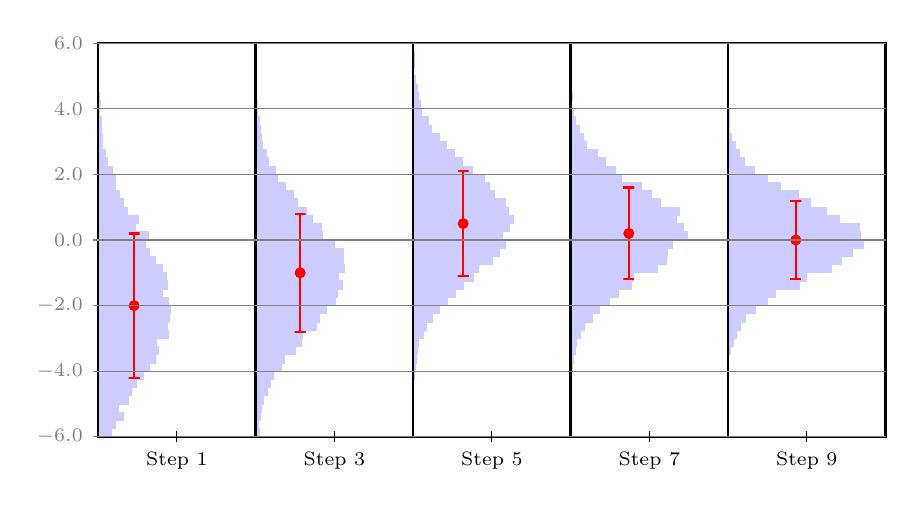
\begin{tikzpicture}
\begin{scope}[]
\pgfpathmoveto{ \pgfpointadd{\pgfpointxy {0.0} {0.0}} {\pgfpoint{0cm}{0.0cm}} }
\pgfpathlineto{ \pgfpointadd{\pgfpointxy {0.0} {0.0}} {\pgfpoint{2.0cm}{0.0cm}} }
\pgfpathlineto{ \pgfpointadd{\pgfpointxy {0.0} {0.0}} {\pgfpoint{2.0cm}{5.0cm}} }
\pgfpathlineto{ \pgfpointadd{\pgfpointxy {0.0} {0.0}} {\pgfpoint{0cm}{5.0cm}} }
\pgfpathclose
\pgfusepath{  clip, }
\begin{scope}[shift={(0.0,0.0)}]
\pgfsetxvec{\pgfpoint{0.002cm}{0cm}}
\pgfsetyvec{\pgfpoint{0cm}{0.41666666cm}}
\begin{scope}[shift={(-0.0,6.0)}]
\begin{scope}[fill=blue!20,draw=blue!20]
\pgfpathmoveto{ \pgfpointxy {0.0} {6.0}}
\pgfpathlineto{ \pgfpointxy {0.0} {6.0}}
\pgfpathlineto{ \pgfpointxy {0.0} {6.0}}
\pgfpathlineto{ \pgfpointxy {0.0} {5.75}}
\pgfpathlineto{ \pgfpointxy {2.0} {5.75}}
\pgfpathlineto{ \pgfpointxy {2.0} {5.5}}
\pgfpathlineto{ \pgfpointxy {4.0} {5.5}}
\pgfpathlineto{ \pgfpointxy {4.0} {5.25}}
\pgfpathlineto{ \pgfpointxy {0.0} {5.25}}
\pgfpathlineto{ \pgfpointxy {0.0} {5.0}}
\pgfpathlineto{ \pgfpointxy {3.0} {5.0}}
\pgfpathlineto{ \pgfpointxy {3.0} {4.75}}
\pgfpathlineto{ \pgfpointxy {3.0} {4.75}}
\pgfpathlineto{ \pgfpointxy {3.0} {4.5}}
\pgfpathlineto{ \pgfpointxy {8.0} {4.5}}
\pgfpathlineto{ \pgfpointxy {8.0} {4.25}}
\pgfpathlineto{ \pgfpointxy {15.0} {4.25}}
\pgfpathlineto{ \pgfpointxy {15.0} {4.0}}
\pgfpathlineto{ \pgfpointxy {11.0} {4.0}}
\pgfpathlineto{ \pgfpointxy {11.0} {3.75}}
\pgfpathlineto{ \pgfpointxy {20.0} {3.75}}
\pgfpathlineto{ \pgfpointxy {20.0} {3.5}}
\pgfpathlineto{ \pgfpointxy {22.0} {3.5}}
\pgfpathlineto{ \pgfpointxy {22.0} {3.25}}
\pgfpathlineto{ \pgfpointxy {25.0} {3.25}}
\pgfpathlineto{ \pgfpointxy {25.0} {3.0}}
\pgfpathlineto{ \pgfpointxy {30.0} {3.0}}
\pgfpathlineto{ \pgfpointxy {30.0} {2.75}}
\pgfpathlineto{ \pgfpointxy {46.0} {2.75}}
\pgfpathlineto{ \pgfpointxy {46.0} {2.5}}
\pgfpathlineto{ \pgfpointxy {56.0} {2.5}}
\pgfpathlineto{ \pgfpointxy {56.0} {2.25}}
\pgfpathlineto{ \pgfpointxy {90.0} {2.25}}
\pgfpathlineto{ \pgfpointxy {90.0} {2.0}}
\pgfpathlineto{ \pgfpointxy {110.0} {2.0}}
\pgfpathlineto{ \pgfpointxy {110.0} {1.75}}
\pgfpathlineto{ \pgfpointxy {107.0} {1.75}}
\pgfpathlineto{ \pgfpointxy {107.0} {1.5}}
\pgfpathlineto{ \pgfpointxy {135.0} {1.5}}
\pgfpathlineto{ \pgfpointxy {135.0} {1.25}}
\pgfpathlineto{ \pgfpointxy {158.0} {1.25}}
\pgfpathlineto{ \pgfpointxy {158.0} {1.0}}
\pgfpathlineto{ \pgfpointxy {186.0} {1.0}}
\pgfpathlineto{ \pgfpointxy {186.0} {0.75}}
\pgfpathlineto{ \pgfpointxy {256.0} {0.75}}
\pgfpathlineto{ \pgfpointxy {256.0} {0.5}}
\pgfpathlineto{ \pgfpointxy {238.0} {0.5}}
\pgfpathlineto{ \pgfpointxy {238.0} {0.25}}
\pgfpathlineto{ \pgfpointxy {319.0} {0.25}}
\pgfpathlineto{ \pgfpointxy {319.0} {0.0}}
\pgfpathlineto{ \pgfpointxy {300.0} {0.0}}
\pgfpathlineto{ \pgfpointxy {300.0} {-0.25}}
\pgfpathlineto{ \pgfpointxy {328.0} {-0.25}}
\pgfpathlineto{ \pgfpointxy {328.0} {-0.5}}
\pgfpathlineto{ \pgfpointxy {364.0} {-0.5}}
\pgfpathlineto{ \pgfpointxy {364.0} {-0.75}}
\pgfpathlineto{ \pgfpointxy {411.0} {-0.75}}
\pgfpathlineto{ \pgfpointxy {411.0} {-1.0}}
\pgfpathlineto{ \pgfpointxy {431.0} {-1.0}}
\pgfpathlineto{ \pgfpointxy {431.0} {-1.25}}
\pgfpathlineto{ \pgfpointxy {442.0} {-1.25}}
\pgfpathlineto{ \pgfpointxy {442.0} {-1.5}}
\pgfpathlineto{ \pgfpointxy {407.0} {-1.5}}
\pgfpathlineto{ \pgfpointxy {407.0} {-1.75}}
\pgfpathlineto{ \pgfpointxy {444.0} {-1.75}}
\pgfpathlineto{ \pgfpointxy {444.0} {-2.0}}
\pgfpathlineto{ \pgfpointxy {457.0} {-2.0}}
\pgfpathlineto{ \pgfpointxy {457.0} {-2.25}}
\pgfpathlineto{ \pgfpointxy {455.0} {-2.25}}
\pgfpathlineto{ \pgfpointxy {455.0} {-2.5}}
\pgfpathlineto{ \pgfpointxy {439.0} {-2.5}}
\pgfpathlineto{ \pgfpointxy {439.0} {-2.75}}
\pgfpathlineto{ \pgfpointxy {448.0} {-2.75}}
\pgfpathlineto{ \pgfpointxy {448.0} {-3.0}}
\pgfpathlineto{ \pgfpointxy {373.0} {-3.0}}
\pgfpathlineto{ \pgfpointxy {373.0} {-3.25}}
\pgfpathlineto{ \pgfpointxy {385.0} {-3.25}}
\pgfpathlineto{ \pgfpointxy {385.0} {-3.5}}
\pgfpathlineto{ \pgfpointxy {362.0} {-3.5}}
\pgfpathlineto{ \pgfpointxy {362.0} {-3.75}}
\pgfpathlineto{ \pgfpointxy {325.0} {-3.75}}
\pgfpathlineto{ \pgfpointxy {325.0} {-4.0}}
\pgfpathlineto{ \pgfpointxy {289.0} {-4.0}}
\pgfpathlineto{ \pgfpointxy {289.0} {-4.25}}
\pgfpathlineto{ \pgfpointxy {243.0} {-4.25}}
\pgfpathlineto{ \pgfpointxy {243.0} {-4.5}}
\pgfpathlineto{ \pgfpointxy {209.0} {-4.5}}
\pgfpathlineto{ \pgfpointxy {209.0} {-4.75}}
\pgfpathlineto{ \pgfpointxy {191.0} {-4.75}}
\pgfpathlineto{ \pgfpointxy {191.0} {-5.0}}
\pgfpathlineto{ \pgfpointxy {132.0} {-5.0}}
\pgfpathlineto{ \pgfpointxy {132.0} {-5.25}}
\pgfpathlineto{ \pgfpointxy {158.0} {-5.25}}
\pgfpathlineto{ \pgfpointxy {158.0} {-5.5}}
\pgfpathlineto{ \pgfpointxy {113.0} {-5.5}}
\pgfpathlineto{ \pgfpointxy {113.0} {-5.75}}
\pgfpathlineto{ \pgfpointxy {86.0} {-5.75}}
\pgfpathlineto{ \pgfpointxy {86.0} {-6.0}}
\pgfpathlineto{ \pgfpointxy {0.0} {-6.0}}
\pgfusepath{ stroke, fill, }
\end{scope}
\end{scope}
\pgfsetxvec{\pgfpoint{1cm}{0cm}}
\pgfsetyvec{\pgfpoint{0cm}{1cm}}
\end{scope}
\end{scope}
\begin{scope}[shift={(0.0,0.0)}]
\pgfsetxvec{\pgfpoint{0.002cm}{0cm}}
\pgfsetyvec{\pgfpoint{0cm}{0.41666666cm}}
\begin{scope}[shift={(-0.0,6.0)}]
\begin{scope}[red,fill=red,thick]
\pgfpathmoveto{ \pgfpointadd{\pgfpointxy {228.5} {0.20000005}} {\pgfpoint{-2pt}{0}} }
\pgfpathlineto{ \pgfpointadd{\pgfpointxy {228.5} {0.20000005}} {\pgfpoint{2pt}{0}} }
\pgfpathlineto{ \pgfpointadd{\pgfpointxy {228.5} {0.20000005}} {\pgfpoint{0pt}{0}} }
\pgfpathlineto{ \pgfpointadd{\pgfpointxy {228.5} {-4.2}} {\pgfpoint{0pt}{0}} }
\pgfpathlineto{ \pgfpointadd{\pgfpointxy {228.5} {-4.2}} {\pgfpoint{-2pt}{0}} }
\pgfpathlineto{ \pgfpointadd{\pgfpointxy {228.5} {-4.2}} {\pgfpoint{2pt}{0}} }
\pgfusepath{ stroke, }
\node at (228.5,-2.0) [red,fill=red,thick,circle,inner sep=0.0pt,minimum width =4.0pt,minimum height=4.0pt] {};
\end{scope}
\end{scope}
\pgfsetxvec{\pgfpoint{1cm}{0cm}}
\pgfsetyvec{\pgfpoint{0cm}{1cm}}
\end{scope}
\begin{scope}[shift={(0.0,0.0)}]
\pgfsetxvec{\pgfpoint{0.002cm}{0cm}}
\pgfsetyvec{\pgfpoint{0cm}{0.41666666cm}}
\begin{scope}[shift={(-0.0,6.0)}]
\begin{scope}[thick,black,fill=white]
\pgfpathmoveto{ \pgfpointxy {0.0} {-6.0}}
\pgfpathlineto{ \pgfpointxy {1000.0} {-6.0}}
\pgfpathlineto{ \pgfpointxy {1000.0} {6.0}}
\pgfpathlineto{ \pgfpointxy {0.0} {6.0}}
\pgfpathclose
\pgfusepath{ stroke, }
\end{scope}
\begin{scope}[yshift=0cm]
\end{scope}
\begin{scope}[xshift=0cm]
\end{scope}
\end{scope}
\pgfsetxvec{\pgfpoint{1cm}{0cm}}
\pgfsetyvec{\pgfpoint{0cm}{1cm}}
\end{scope}
\begin{scope}[]
\pgfpathmoveto{ \pgfpointadd{\pgfpointxy {0.0} {0.0}} {\pgfpoint{2cm}{0.0cm}} }
\pgfpathlineto{ \pgfpointadd{\pgfpointxy {0.0} {0.0}} {\pgfpoint{4.0cm}{0.0cm}} }
\pgfpathlineto{ \pgfpointadd{\pgfpointxy {0.0} {0.0}} {\pgfpoint{4.0cm}{5.0cm}} }
\pgfpathlineto{ \pgfpointadd{\pgfpointxy {0.0} {0.0}} {\pgfpoint{2cm}{5.0cm}} }
\pgfpathclose
\pgfusepath{  clip, }
\begin{scope}[shift={(2.0,0.0)}]
\pgfsetxvec{\pgfpoint{0.002cm}{0cm}}
\pgfsetyvec{\pgfpoint{0cm}{0.41666666cm}}
\begin{scope}[shift={(-0.0,6.0)}]
\begin{scope}[fill=blue!20,draw=blue!20]
\pgfpathmoveto{ \pgfpointxy {0.0} {6.0}}
\pgfpathlineto{ \pgfpointxy {0.0} {6.0}}
\pgfpathlineto{ \pgfpointxy {0.0} {6.0}}
\pgfpathlineto{ \pgfpointxy {0.0} {5.75}}
\pgfpathlineto{ \pgfpointxy {1.0} {5.75}}
\pgfpathlineto{ \pgfpointxy {1.0} {5.5}}
\pgfpathlineto{ \pgfpointxy {0.0} {5.5}}
\pgfpathlineto{ \pgfpointxy {0.0} {5.25}}
\pgfpathlineto{ \pgfpointxy {2.0} {5.25}}
\pgfpathlineto{ \pgfpointxy {2.0} {5.0}}
\pgfpathlineto{ \pgfpointxy {3.0} {5.0}}
\pgfpathlineto{ \pgfpointxy {3.0} {4.75}}
\pgfpathlineto{ \pgfpointxy {5.0} {4.75}}
\pgfpathlineto{ \pgfpointxy {5.0} {4.5}}
\pgfpathlineto{ \pgfpointxy {5.0} {4.5}}
\pgfpathlineto{ \pgfpointxy {5.0} {4.25}}
\pgfpathlineto{ \pgfpointxy {12.0} {4.25}}
\pgfpathlineto{ \pgfpointxy {12.0} {4.0}}
\pgfpathlineto{ \pgfpointxy {10.0} {4.0}}
\pgfpathlineto{ \pgfpointxy {10.0} {3.75}}
\pgfpathlineto{ \pgfpointxy {24.0} {3.75}}
\pgfpathlineto{ \pgfpointxy {24.0} {3.5}}
\pgfpathlineto{ \pgfpointxy {29.0} {3.5}}
\pgfpathlineto{ \pgfpointxy {29.0} {3.25}}
\pgfpathlineto{ \pgfpointxy {37.0} {3.25}}
\pgfpathlineto{ \pgfpointxy {37.0} {3.0}}
\pgfpathlineto{ \pgfpointxy {43.0} {3.0}}
\pgfpathlineto{ \pgfpointxy {43.0} {2.75}}
\pgfpathlineto{ \pgfpointxy {71.0} {2.75}}
\pgfpathlineto{ \pgfpointxy {71.0} {2.5}}
\pgfpathlineto{ \pgfpointxy {83.0} {2.5}}
\pgfpathlineto{ \pgfpointxy {83.0} {2.25}}
\pgfpathlineto{ \pgfpointxy {124.0} {2.25}}
\pgfpathlineto{ \pgfpointxy {124.0} {2.0}}
\pgfpathlineto{ \pgfpointxy {141.0} {2.0}}
\pgfpathlineto{ \pgfpointxy {141.0} {1.75}}
\pgfpathlineto{ \pgfpointxy {192.0} {1.75}}
\pgfpathlineto{ \pgfpointxy {192.0} {1.5}}
\pgfpathlineto{ \pgfpointxy {238.0} {1.5}}
\pgfpathlineto{ \pgfpointxy {238.0} {1.25}}
\pgfpathlineto{ \pgfpointxy {267.0} {1.25}}
\pgfpathlineto{ \pgfpointxy {267.0} {1.0}}
\pgfpathlineto{ \pgfpointxy {324.0} {1.0}}
\pgfpathlineto{ \pgfpointxy {324.0} {0.75}}
\pgfpathlineto{ \pgfpointxy {359.0} {0.75}}
\pgfpathlineto{ \pgfpointxy {359.0} {0.5}}
\pgfpathlineto{ \pgfpointxy {419.0} {0.5}}
\pgfpathlineto{ \pgfpointxy {419.0} {0.25}}
\pgfpathlineto{ \pgfpointxy {424.0} {0.25}}
\pgfpathlineto{ \pgfpointxy {424.0} {0.0}}
\pgfpathlineto{ \pgfpointxy {498.0} {0.0}}
\pgfpathlineto{ \pgfpointxy {498.0} {-0.25}}
\pgfpathlineto{ \pgfpointxy {555.0} {-0.25}}
\pgfpathlineto{ \pgfpointxy {555.0} {-0.5}}
\pgfpathlineto{ \pgfpointxy {556.0} {-0.5}}
\pgfpathlineto{ \pgfpointxy {556.0} {-0.75}}
\pgfpathlineto{ \pgfpointxy {566.0} {-0.75}}
\pgfpathlineto{ \pgfpointxy {566.0} {-1.0}}
\pgfpathlineto{ \pgfpointxy {528.0} {-1.0}}
\pgfpathlineto{ \pgfpointxy {528.0} {-1.25}}
\pgfpathlineto{ \pgfpointxy {550.0} {-1.25}}
\pgfpathlineto{ \pgfpointxy {550.0} {-1.5}}
\pgfpathlineto{ \pgfpointxy {523.0} {-1.5}}
\pgfpathlineto{ \pgfpointxy {523.0} {-1.75}}
\pgfpathlineto{ \pgfpointxy {509.0} {-1.75}}
\pgfpathlineto{ \pgfpointxy {509.0} {-2.0}}
\pgfpathlineto{ \pgfpointxy {451.0} {-2.0}}
\pgfpathlineto{ \pgfpointxy {451.0} {-2.25}}
\pgfpathlineto{ \pgfpointxy {403.0} {-2.25}}
\pgfpathlineto{ \pgfpointxy {403.0} {-2.5}}
\pgfpathlineto{ \pgfpointxy {387.0} {-2.5}}
\pgfpathlineto{ \pgfpointxy {387.0} {-2.75}}
\pgfpathlineto{ \pgfpointxy {298.0} {-2.75}}
\pgfpathlineto{ \pgfpointxy {298.0} {-3.0}}
\pgfpathlineto{ \pgfpointxy {294.0} {-3.0}}
\pgfpathlineto{ \pgfpointxy {294.0} {-3.25}}
\pgfpathlineto{ \pgfpointxy {254.0} {-3.25}}
\pgfpathlineto{ \pgfpointxy {254.0} {-3.5}}
\pgfpathlineto{ \pgfpointxy {183.0} {-3.5}}
\pgfpathlineto{ \pgfpointxy {183.0} {-3.75}}
\pgfpathlineto{ \pgfpointxy {167.0} {-3.75}}
\pgfpathlineto{ \pgfpointxy {167.0} {-4.0}}
\pgfpathlineto{ \pgfpointxy {116.0} {-4.0}}
\pgfpathlineto{ \pgfpointxy {116.0} {-4.25}}
\pgfpathlineto{ \pgfpointxy {94.0} {-4.25}}
\pgfpathlineto{ \pgfpointxy {94.0} {-4.5}}
\pgfpathlineto{ \pgfpointxy {75.0} {-4.5}}
\pgfpathlineto{ \pgfpointxy {75.0} {-4.75}}
\pgfpathlineto{ \pgfpointxy {48.0} {-4.75}}
\pgfpathlineto{ \pgfpointxy {48.0} {-5.0}}
\pgfpathlineto{ \pgfpointxy {40.0} {-5.0}}
\pgfpathlineto{ \pgfpointxy {40.0} {-5.25}}
\pgfpathlineto{ \pgfpointxy {32.0} {-5.25}}
\pgfpathlineto{ \pgfpointxy {32.0} {-5.5}}
\pgfpathlineto{ \pgfpointxy {17.0} {-5.5}}
\pgfpathlineto{ \pgfpointxy {17.0} {-5.75}}
\pgfpathlineto{ \pgfpointxy {23.0} {-5.75}}
\pgfpathlineto{ \pgfpointxy {23.0} {-6.0}}
\pgfpathlineto{ \pgfpointxy {0.0} {-6.0}}
\pgfusepath{ stroke, fill, }
\end{scope}
\end{scope}
\pgfsetxvec{\pgfpoint{1cm}{0cm}}
\pgfsetyvec{\pgfpoint{0cm}{1cm}}
\end{scope}
\end{scope}
\begin{scope}[shift={(2.0,0.0)}]
\pgfsetxvec{\pgfpoint{0.002cm}{0cm}}
\pgfsetyvec{\pgfpoint{0cm}{0.41666666cm}}
\begin{scope}[shift={(-0.0,6.0)}]
\begin{scope}[red,fill=red,thick]
\pgfpathmoveto{ \pgfpointadd{\pgfpointxy {283.0} {0.79999995}} {\pgfpoint{-2pt}{0}} }
\pgfpathlineto{ \pgfpointadd{\pgfpointxy {283.0} {0.79999995}} {\pgfpoint{2pt}{0}} }
\pgfpathlineto{ \pgfpointadd{\pgfpointxy {283.0} {0.79999995}} {\pgfpoint{0pt}{0}} }
\pgfpathlineto{ \pgfpointadd{\pgfpointxy {283.0} {-2.8}} {\pgfpoint{0pt}{0}} }
\pgfpathlineto{ \pgfpointadd{\pgfpointxy {283.0} {-2.8}} {\pgfpoint{-2pt}{0}} }
\pgfpathlineto{ \pgfpointadd{\pgfpointxy {283.0} {-2.8}} {\pgfpoint{2pt}{0}} }
\pgfusepath{ stroke, }
\node at (283.0,-1.0) [red,fill=red,thick,circle,inner sep=0.0pt,minimum width =4.0pt,minimum height=4.0pt] {};
\end{scope}
\end{scope}
\pgfsetxvec{\pgfpoint{1cm}{0cm}}
\pgfsetyvec{\pgfpoint{0cm}{1cm}}
\end{scope}
\begin{scope}[shift={(2.0,0.0)}]
\pgfsetxvec{\pgfpoint{0.002cm}{0cm}}
\pgfsetyvec{\pgfpoint{0cm}{0.41666666cm}}
\begin{scope}[shift={(-0.0,6.0)}]
\begin{scope}[thick,black,fill=white]
\pgfpathmoveto{ \pgfpointxy {0.0} {-6.0}}
\pgfpathlineto{ \pgfpointxy {1000.0} {-6.0}}
\pgfpathlineto{ \pgfpointxy {1000.0} {6.0}}
\pgfpathlineto{ \pgfpointxy {0.0} {6.0}}
\pgfpathclose
\pgfusepath{ stroke, }
\end{scope}
\begin{scope}[yshift=0cm]
\end{scope}
\begin{scope}[xshift=0cm]
\end{scope}
\end{scope}
\pgfsetxvec{\pgfpoint{1cm}{0cm}}
\pgfsetyvec{\pgfpoint{0cm}{1cm}}
\end{scope}
\begin{scope}[]
\pgfpathmoveto{ \pgfpointadd{\pgfpointxy {0.0} {0.0}} {\pgfpoint{4cm}{0.0cm}} }
\pgfpathlineto{ \pgfpointadd{\pgfpointxy {0.0} {0.0}} {\pgfpoint{6.0cm}{0.0cm}} }
\pgfpathlineto{ \pgfpointadd{\pgfpointxy {0.0} {0.0}} {\pgfpoint{6.0cm}{5.0cm}} }
\pgfpathlineto{ \pgfpointadd{\pgfpointxy {0.0} {0.0}} {\pgfpoint{4cm}{5.0cm}} }
\pgfpathclose
\pgfusepath{  clip, }
\begin{scope}[shift={(4.0,0.0)}]
\pgfsetxvec{\pgfpoint{0.002cm}{0cm}}
\pgfsetyvec{\pgfpoint{0cm}{0.41666666cm}}
\begin{scope}[shift={(-0.0,6.0)}]
\begin{scope}[fill=blue!20,draw=blue!20]
\pgfpathmoveto{ \pgfpointxy {0.0} {6.0}}
\pgfpathlineto{ \pgfpointxy {2.0} {6.0}}
\pgfpathlineto{ \pgfpointxy {2.0} {6.0}}
\pgfpathlineto{ \pgfpointxy {2.0} {5.75}}
\pgfpathlineto{ \pgfpointxy {8.0} {5.75}}
\pgfpathlineto{ \pgfpointxy {8.0} {5.5}}
\pgfpathlineto{ \pgfpointxy {10.0} {5.5}}
\pgfpathlineto{ \pgfpointxy {10.0} {5.25}}
\pgfpathlineto{ \pgfpointxy {5.0} {5.25}}
\pgfpathlineto{ \pgfpointxy {5.0} {5.0}}
\pgfpathlineto{ \pgfpointxy {15.0} {5.0}}
\pgfpathlineto{ \pgfpointxy {15.0} {4.75}}
\pgfpathlineto{ \pgfpointxy {29.0} {4.75}}
\pgfpathlineto{ \pgfpointxy {29.0} {4.5}}
\pgfpathlineto{ \pgfpointxy {31.0} {4.5}}
\pgfpathlineto{ \pgfpointxy {31.0} {4.25}}
\pgfpathlineto{ \pgfpointxy {46.0} {4.25}}
\pgfpathlineto{ \pgfpointxy {46.0} {4.0}}
\pgfpathlineto{ \pgfpointxy {52.0} {4.0}}
\pgfpathlineto{ \pgfpointxy {52.0} {3.75}}
\pgfpathlineto{ \pgfpointxy {97.0} {3.75}}
\pgfpathlineto{ \pgfpointxy {97.0} {3.5}}
\pgfpathlineto{ \pgfpointxy {115.0} {3.5}}
\pgfpathlineto{ \pgfpointxy {115.0} {3.25}}
\pgfpathlineto{ \pgfpointxy {169.0} {3.25}}
\pgfpathlineto{ \pgfpointxy {169.0} {3.0}}
\pgfpathlineto{ \pgfpointxy {209.0} {3.0}}
\pgfpathlineto{ \pgfpointxy {209.0} {2.75}}
\pgfpathlineto{ \pgfpointxy {261.0} {2.75}}
\pgfpathlineto{ \pgfpointxy {261.0} {2.5}}
\pgfpathlineto{ \pgfpointxy {312.0} {2.5}}
\pgfpathlineto{ \pgfpointxy {312.0} {2.25}}
\pgfpathlineto{ \pgfpointxy {375.0} {2.25}}
\pgfpathlineto{ \pgfpointxy {375.0} {2.0}}
\pgfpathlineto{ \pgfpointxy {451.0} {2.0}}
\pgfpathlineto{ \pgfpointxy {451.0} {1.75}}
\pgfpathlineto{ \pgfpointxy {484.0} {1.75}}
\pgfpathlineto{ \pgfpointxy {484.0} {1.5}}
\pgfpathlineto{ \pgfpointxy {516.0} {1.5}}
\pgfpathlineto{ \pgfpointxy {516.0} {1.25}}
\pgfpathlineto{ \pgfpointxy {586.0} {1.25}}
\pgfpathlineto{ \pgfpointxy {586.0} {1.0}}
\pgfpathlineto{ \pgfpointxy {603.0} {1.0}}
\pgfpathlineto{ \pgfpointxy {603.0} {0.75}}
\pgfpathlineto{ \pgfpointxy {636.0} {0.75}}
\pgfpathlineto{ \pgfpointxy {636.0} {0.5}}
\pgfpathlineto{ \pgfpointxy {609.0} {0.5}}
\pgfpathlineto{ \pgfpointxy {609.0} {0.25}}
\pgfpathlineto{ \pgfpointxy {570.0} {0.25}}
\pgfpathlineto{ \pgfpointxy {570.0} {0.0}}
\pgfpathlineto{ \pgfpointxy {588.0} {0.0}}
\pgfpathlineto{ \pgfpointxy {588.0} {-0.25}}
\pgfpathlineto{ \pgfpointxy {548.0} {-0.25}}
\pgfpathlineto{ \pgfpointxy {548.0} {-0.5}}
\pgfpathlineto{ \pgfpointxy {506.0} {-0.5}}
\pgfpathlineto{ \pgfpointxy {506.0} {-0.75}}
\pgfpathlineto{ \pgfpointxy {412.0} {-0.75}}
\pgfpathlineto{ \pgfpointxy {412.0} {-1.0}}
\pgfpathlineto{ \pgfpointxy {384.0} {-1.0}}
\pgfpathlineto{ \pgfpointxy {384.0} {-1.25}}
\pgfpathlineto{ \pgfpointxy {318.0} {-1.25}}
\pgfpathlineto{ \pgfpointxy {318.0} {-1.5}}
\pgfpathlineto{ \pgfpointxy {272.0} {-1.5}}
\pgfpathlineto{ \pgfpointxy {272.0} {-1.75}}
\pgfpathlineto{ \pgfpointxy {216.0} {-1.75}}
\pgfpathlineto{ \pgfpointxy {216.0} {-2.0}}
\pgfpathlineto{ \pgfpointxy {167.0} {-2.0}}
\pgfpathlineto{ \pgfpointxy {167.0} {-2.25}}
\pgfpathlineto{ \pgfpointxy {124.0} {-2.25}}
\pgfpathlineto{ \pgfpointxy {124.0} {-2.5}}
\pgfpathlineto{ \pgfpointxy {83.0} {-2.5}}
\pgfpathlineto{ \pgfpointxy {83.0} {-2.75}}
\pgfpathlineto{ \pgfpointxy {68.0} {-2.75}}
\pgfpathlineto{ \pgfpointxy {68.0} {-3.0}}
\pgfpathlineto{ \pgfpointxy {35.0} {-3.0}}
\pgfpathlineto{ \pgfpointxy {35.0} {-3.25}}
\pgfpathlineto{ \pgfpointxy {27.0} {-3.25}}
\pgfpathlineto{ \pgfpointxy {27.0} {-3.5}}
\pgfpathlineto{ \pgfpointxy {23.0} {-3.5}}
\pgfpathlineto{ \pgfpointxy {23.0} {-3.75}}
\pgfpathlineto{ \pgfpointxy {15.0} {-3.75}}
\pgfpathlineto{ \pgfpointxy {15.0} {-4.0}}
\pgfpathlineto{ \pgfpointxy {10.0} {-4.0}}
\pgfpathlineto{ \pgfpointxy {10.0} {-4.25}}
\pgfpathlineto{ \pgfpointxy {2.0} {-4.25}}
\pgfpathlineto{ \pgfpointxy {2.0} {-4.5}}
\pgfpathlineto{ \pgfpointxy {3.0} {-4.5}}
\pgfpathlineto{ \pgfpointxy {3.0} {-4.75}}
\pgfpathlineto{ \pgfpointxy {2.0} {-4.75}}
\pgfpathlineto{ \pgfpointxy {2.0} {-5.0}}
\pgfpathlineto{ \pgfpointxy {3.0} {-5.0}}
\pgfpathlineto{ \pgfpointxy {3.0} {-5.25}}
\pgfpathlineto{ \pgfpointxy {0.0} {-5.25}}
\pgfpathlineto{ \pgfpointxy {0.0} {-5.5}}
\pgfpathlineto{ \pgfpointxy {0.0} {-5.5}}
\pgfpathlineto{ \pgfpointxy {0.0} {-5.75}}
\pgfpathlineto{ \pgfpointxy {0.0} {-5.75}}
\pgfpathlineto{ \pgfpointxy {0.0} {-6.0}}
\pgfpathlineto{ \pgfpointxy {0.0} {-6.0}}
\pgfusepath{ stroke, fill, }
\end{scope}
\end{scope}
\pgfsetxvec{\pgfpoint{1cm}{0cm}}
\pgfsetyvec{\pgfpoint{0cm}{1cm}}
\end{scope}
\end{scope}
\begin{scope}[shift={(4.0,0.0)}]
\pgfsetxvec{\pgfpoint{0.002cm}{0cm}}
\pgfsetyvec{\pgfpoint{0cm}{0.41666666cm}}
\begin{scope}[shift={(-0.0,6.0)}]
\begin{scope}[red,fill=red,thick]
\pgfpathmoveto{ \pgfpointadd{\pgfpointxy {318.0} {2.1}} {\pgfpoint{-2pt}{0}} }
\pgfpathlineto{ \pgfpointadd{\pgfpointxy {318.0} {2.1}} {\pgfpoint{2pt}{0}} }
\pgfpathlineto{ \pgfpointadd{\pgfpointxy {318.0} {2.1}} {\pgfpoint{0pt}{0}} }
\pgfpathlineto{ \pgfpointadd{\pgfpointxy {318.0} {-1.1}} {\pgfpoint{0pt}{0}} }
\pgfpathlineto{ \pgfpointadd{\pgfpointxy {318.0} {-1.1}} {\pgfpoint{-2pt}{0}} }
\pgfpathlineto{ \pgfpointadd{\pgfpointxy {318.0} {-1.1}} {\pgfpoint{2pt}{0}} }
\pgfusepath{ stroke, }
\node at (318.0,0.5) [red,fill=red,thick,circle,inner sep=0.0pt,minimum width =4.0pt,minimum height=4.0pt] {};
\end{scope}
\end{scope}
\pgfsetxvec{\pgfpoint{1cm}{0cm}}
\pgfsetyvec{\pgfpoint{0cm}{1cm}}
\end{scope}
\begin{scope}[shift={(4.0,0.0)}]
\pgfsetxvec{\pgfpoint{0.002cm}{0cm}}
\pgfsetyvec{\pgfpoint{0cm}{0.41666666cm}}
\begin{scope}[shift={(-0.0,6.0)}]
\begin{scope}[thick,black,fill=white]
\pgfpathmoveto{ \pgfpointxy {0.0} {-6.0}}
\pgfpathlineto{ \pgfpointxy {1000.0} {-6.0}}
\pgfpathlineto{ \pgfpointxy {1000.0} {6.0}}
\pgfpathlineto{ \pgfpointxy {0.0} {6.0}}
\pgfpathclose
\pgfusepath{ stroke, }
\end{scope}
\begin{scope}[yshift=0cm]
\end{scope}
\begin{scope}[xshift=0cm]
\end{scope}
\end{scope}
\pgfsetxvec{\pgfpoint{1cm}{0cm}}
\pgfsetyvec{\pgfpoint{0cm}{1cm}}
\end{scope}
\begin{scope}[]
\pgfpathmoveto{ \pgfpointadd{\pgfpointxy {0.0} {0.0}} {\pgfpoint{6cm}{0.0cm}} }
\pgfpathlineto{ \pgfpointadd{\pgfpointxy {0.0} {0.0}} {\pgfpoint{8.0cm}{0.0cm}} }
\pgfpathlineto{ \pgfpointadd{\pgfpointxy {0.0} {0.0}} {\pgfpoint{8.0cm}{5.0cm}} }
\pgfpathlineto{ \pgfpointadd{\pgfpointxy {0.0} {0.0}} {\pgfpoint{6cm}{5.0cm}} }
\pgfpathclose
\pgfusepath{  clip, }
\begin{scope}[shift={(6.0,0.0)}]
\pgfsetxvec{\pgfpoint{0.002cm}{0cm}}
\pgfsetyvec{\pgfpoint{0cm}{0.41666666cm}}
\begin{scope}[shift={(-0.0,6.0)}]
\begin{scope}[fill=blue!20,draw=blue!20]
\pgfpathmoveto{ \pgfpointxy {0.0} {6.0}}
\pgfpathlineto{ \pgfpointxy {0.0} {6.0}}
\pgfpathlineto{ \pgfpointxy {0.0} {6.0}}
\pgfpathlineto{ \pgfpointxy {0.0} {5.75}}
\pgfpathlineto{ \pgfpointxy {0.0} {5.75}}
\pgfpathlineto{ \pgfpointxy {0.0} {5.5}}
\pgfpathlineto{ \pgfpointxy {0.0} {5.5}}
\pgfpathlineto{ \pgfpointxy {0.0} {5.25}}
\pgfpathlineto{ \pgfpointxy {1.0} {5.25}}
\pgfpathlineto{ \pgfpointxy {1.0} {5.0}}
\pgfpathlineto{ \pgfpointxy {3.0} {5.0}}
\pgfpathlineto{ \pgfpointxy {3.0} {4.75}}
\pgfpathlineto{ \pgfpointxy {8.0} {4.75}}
\pgfpathlineto{ \pgfpointxy {8.0} {4.5}}
\pgfpathlineto{ \pgfpointxy {9.0} {4.5}}
\pgfpathlineto{ \pgfpointxy {9.0} {4.25}}
\pgfpathlineto{ \pgfpointxy {8.0} {4.25}}
\pgfpathlineto{ \pgfpointxy {8.0} {4.0}}
\pgfpathlineto{ \pgfpointxy {19.0} {4.0}}
\pgfpathlineto{ \pgfpointxy {19.0} {3.75}}
\pgfpathlineto{ \pgfpointxy {31.0} {3.75}}
\pgfpathlineto{ \pgfpointxy {31.0} {3.5}}
\pgfpathlineto{ \pgfpointxy {55.0} {3.5}}
\pgfpathlineto{ \pgfpointxy {55.0} {3.25}}
\pgfpathlineto{ \pgfpointxy {82.0} {3.25}}
\pgfpathlineto{ \pgfpointxy {82.0} {3.0}}
\pgfpathlineto{ \pgfpointxy {100.0} {3.0}}
\pgfpathlineto{ \pgfpointxy {100.0} {2.75}}
\pgfpathlineto{ \pgfpointxy {172.0} {2.75}}
\pgfpathlineto{ \pgfpointxy {172.0} {2.5}}
\pgfpathlineto{ \pgfpointxy {220.0} {2.5}}
\pgfpathlineto{ \pgfpointxy {220.0} {2.25}}
\pgfpathlineto{ \pgfpointxy {287.0} {2.25}}
\pgfpathlineto{ \pgfpointxy {287.0} {2.0}}
\pgfpathlineto{ \pgfpointxy {321.0} {2.0}}
\pgfpathlineto{ \pgfpointxy {321.0} {1.75}}
\pgfpathlineto{ \pgfpointxy {448.0} {1.75}}
\pgfpathlineto{ \pgfpointxy {448.0} {1.5}}
\pgfpathlineto{ \pgfpointxy {512.0} {1.5}}
\pgfpathlineto{ \pgfpointxy {512.0} {1.25}}
\pgfpathlineto{ \pgfpointxy {571.0} {1.25}}
\pgfpathlineto{ \pgfpointxy {571.0} {1.0}}
\pgfpathlineto{ \pgfpointxy {690.0} {1.0}}
\pgfpathlineto{ \pgfpointxy {690.0} {0.75}}
\pgfpathlineto{ \pgfpointxy {671.0} {0.75}}
\pgfpathlineto{ \pgfpointxy {671.0} {0.5}}
\pgfpathlineto{ \pgfpointxy {715.0} {0.5}}
\pgfpathlineto{ \pgfpointxy {715.0} {0.25}}
\pgfpathlineto{ \pgfpointxy {740.0} {0.25}}
\pgfpathlineto{ \pgfpointxy {740.0} {0.0}}
\pgfpathlineto{ \pgfpointxy {650.0} {0.0}}
\pgfpathlineto{ \pgfpointxy {650.0} {-0.25}}
\pgfpathlineto{ \pgfpointxy {617.0} {-0.25}}
\pgfpathlineto{ \pgfpointxy {617.0} {-0.5}}
\pgfpathlineto{ \pgfpointxy {609.0} {-0.5}}
\pgfpathlineto{ \pgfpointxy {609.0} {-0.75}}
\pgfpathlineto{ \pgfpointxy {550.0} {-0.75}}
\pgfpathlineto{ \pgfpointxy {550.0} {-1.0}}
\pgfpathlineto{ \pgfpointxy {401.0} {-1.0}}
\pgfpathlineto{ \pgfpointxy {401.0} {-1.25}}
\pgfpathlineto{ \pgfpointxy {386.0} {-1.25}}
\pgfpathlineto{ \pgfpointxy {386.0} {-1.5}}
\pgfpathlineto{ \pgfpointxy {301.0} {-1.5}}
\pgfpathlineto{ \pgfpointxy {301.0} {-1.75}}
\pgfpathlineto{ \pgfpointxy {247.0} {-1.75}}
\pgfpathlineto{ \pgfpointxy {247.0} {-2.0}}
\pgfpathlineto{ \pgfpointxy {181.0} {-2.0}}
\pgfpathlineto{ \pgfpointxy {181.0} {-2.25}}
\pgfpathlineto{ \pgfpointxy {140.0} {-2.25}}
\pgfpathlineto{ \pgfpointxy {140.0} {-2.5}}
\pgfpathlineto{ \pgfpointxy {88.0} {-2.5}}
\pgfpathlineto{ \pgfpointxy {88.0} {-2.75}}
\pgfpathlineto{ \pgfpointxy {61.0} {-2.75}}
\pgfpathlineto{ \pgfpointxy {61.0} {-3.0}}
\pgfpathlineto{ \pgfpointxy {37.0} {-3.0}}
\pgfpathlineto{ \pgfpointxy {37.0} {-3.25}}
\pgfpathlineto{ \pgfpointxy {29.0} {-3.25}}
\pgfpathlineto{ \pgfpointxy {29.0} {-3.5}}
\pgfpathlineto{ \pgfpointxy {21.0} {-3.5}}
\pgfpathlineto{ \pgfpointxy {21.0} {-3.75}}
\pgfpathlineto{ \pgfpointxy {9.0} {-3.75}}
\pgfpathlineto{ \pgfpointxy {9.0} {-4.0}}
\pgfpathlineto{ \pgfpointxy {7.0} {-4.0}}
\pgfpathlineto{ \pgfpointxy {7.0} {-4.25}}
\pgfpathlineto{ \pgfpointxy {2.0} {-4.25}}
\pgfpathlineto{ \pgfpointxy {2.0} {-4.5}}
\pgfpathlineto{ \pgfpointxy {1.0} {-4.5}}
\pgfpathlineto{ \pgfpointxy {1.0} {-4.75}}
\pgfpathlineto{ \pgfpointxy {0.0} {-4.75}}
\pgfpathlineto{ \pgfpointxy {0.0} {-5.0}}
\pgfpathlineto{ \pgfpointxy {0.0} {-5.0}}
\pgfpathlineto{ \pgfpointxy {0.0} {-5.25}}
\pgfpathlineto{ \pgfpointxy {0.0} {-5.25}}
\pgfpathlineto{ \pgfpointxy {0.0} {-5.5}}
\pgfpathlineto{ \pgfpointxy {0.0} {-5.5}}
\pgfpathlineto{ \pgfpointxy {0.0} {-5.75}}
\pgfpathlineto{ \pgfpointxy {0.0} {-5.75}}
\pgfpathlineto{ \pgfpointxy {0.0} {-6.0}}
\pgfpathlineto{ \pgfpointxy {0.0} {-6.0}}
\pgfusepath{ stroke, fill, }
\end{scope}
\end{scope}
\pgfsetxvec{\pgfpoint{1cm}{0cm}}
\pgfsetyvec{\pgfpoint{0cm}{1cm}}
\end{scope}
\end{scope}
\begin{scope}[shift={(6.0,0.0)}]
\pgfsetxvec{\pgfpoint{0.002cm}{0cm}}
\pgfsetyvec{\pgfpoint{0cm}{0.41666666cm}}
\begin{scope}[shift={(-0.0,6.0)}]
\begin{scope}[red,fill=red,thick]
\pgfpathmoveto{ \pgfpointadd{\pgfpointxy {370.0} {1.6}} {\pgfpoint{-2pt}{0}} }
\pgfpathlineto{ \pgfpointadd{\pgfpointxy {370.0} {1.6}} {\pgfpoint{2pt}{0}} }
\pgfpathlineto{ \pgfpointadd{\pgfpointxy {370.0} {1.6}} {\pgfpoint{0pt}{0}} }
\pgfpathlineto{ \pgfpointadd{\pgfpointxy {370.0} {-1.1999999}} {\pgfpoint{0pt}{0}} }
\pgfpathlineto{ \pgfpointadd{\pgfpointxy {370.0} {-1.1999999}} {\pgfpoint{-2pt}{0}} }
\pgfpathlineto{ \pgfpointadd{\pgfpointxy {370.0} {-1.1999999}} {\pgfpoint{2pt}{0}} }
\pgfusepath{ stroke, }
\node at (370.0,0.2) [red,fill=red,thick,circle,inner sep=0.0pt,minimum width =4.0pt,minimum height=4.0pt] {};
\end{scope}
\end{scope}
\pgfsetxvec{\pgfpoint{1cm}{0cm}}
\pgfsetyvec{\pgfpoint{0cm}{1cm}}
\end{scope}
\begin{scope}[shift={(6.0,0.0)}]
\pgfsetxvec{\pgfpoint{0.002cm}{0cm}}
\pgfsetyvec{\pgfpoint{0cm}{0.41666666cm}}
\begin{scope}[shift={(-0.0,6.0)}]
\begin{scope}[thick,black,fill=white]
\pgfpathmoveto{ \pgfpointxy {0.0} {-6.0}}
\pgfpathlineto{ \pgfpointxy {1000.0} {-6.0}}
\pgfpathlineto{ \pgfpointxy {1000.0} {6.0}}
\pgfpathlineto{ \pgfpointxy {0.0} {6.0}}
\pgfpathclose
\pgfusepath{ stroke, }
\end{scope}
\begin{scope}[yshift=0cm]
\end{scope}
\begin{scope}[xshift=0cm]
\end{scope}
\end{scope}
\pgfsetxvec{\pgfpoint{1cm}{0cm}}
\pgfsetyvec{\pgfpoint{0cm}{1cm}}
\end{scope}
\begin{scope}[]
\pgfpathmoveto{ \pgfpointadd{\pgfpointxy {0.0} {0.0}} {\pgfpoint{8cm}{0.0cm}} }
\pgfpathlineto{ \pgfpointadd{\pgfpointxy {0.0} {0.0}} {\pgfpoint{10.0cm}{0.0cm}} }
\pgfpathlineto{ \pgfpointadd{\pgfpointxy {0.0} {0.0}} {\pgfpoint{10.0cm}{5.0cm}} }
\pgfpathlineto{ \pgfpointadd{\pgfpointxy {0.0} {0.0}} {\pgfpoint{8cm}{5.0cm}} }
\pgfpathclose
\pgfusepath{  clip, }
\begin{scope}[shift={(8.0,0.0)}]
\pgfsetxvec{\pgfpoint{0.002cm}{0cm}}
\pgfsetyvec{\pgfpoint{0cm}{0.41666666cm}}
\begin{scope}[shift={(-0.0,6.0)}]
\begin{scope}[fill=blue!20,draw=blue!20]
\pgfpathmoveto{ \pgfpointxy {0.0} {6.0}}
\pgfpathlineto{ \pgfpointxy {0.0} {6.0}}
\pgfpathlineto{ \pgfpointxy {0.0} {6.0}}
\pgfpathlineto{ \pgfpointxy {0.0} {5.75}}
\pgfpathlineto{ \pgfpointxy {0.0} {5.75}}
\pgfpathlineto{ \pgfpointxy {0.0} {5.5}}
\pgfpathlineto{ \pgfpointxy {0.0} {5.5}}
\pgfpathlineto{ \pgfpointxy {0.0} {5.25}}
\pgfpathlineto{ \pgfpointxy {0.0} {5.25}}
\pgfpathlineto{ \pgfpointxy {0.0} {5.0}}
\pgfpathlineto{ \pgfpointxy {0.0} {5.0}}
\pgfpathlineto{ \pgfpointxy {0.0} {4.75}}
\pgfpathlineto{ \pgfpointxy {0.0} {4.75}}
\pgfpathlineto{ \pgfpointxy {0.0} {4.5}}
\pgfpathlineto{ \pgfpointxy {0.0} {4.5}}
\pgfpathlineto{ \pgfpointxy {0.0} {4.25}}
\pgfpathlineto{ \pgfpointxy {2.0} {4.25}}
\pgfpathlineto{ \pgfpointxy {2.0} {4.0}}
\pgfpathlineto{ \pgfpointxy {9.0} {4.0}}
\pgfpathlineto{ \pgfpointxy {9.0} {3.75}}
\pgfpathlineto{ \pgfpointxy {8.0} {3.75}}
\pgfpathlineto{ \pgfpointxy {8.0} {3.5}}
\pgfpathlineto{ \pgfpointxy {11.0} {3.5}}
\pgfpathlineto{ \pgfpointxy {11.0} {3.25}}
\pgfpathlineto{ \pgfpointxy {22.0} {3.25}}
\pgfpathlineto{ \pgfpointxy {22.0} {3.0}}
\pgfpathlineto{ \pgfpointxy {48.0} {3.0}}
\pgfpathlineto{ \pgfpointxy {48.0} {2.75}}
\pgfpathlineto{ \pgfpointxy {73.0} {2.75}}
\pgfpathlineto{ \pgfpointxy {73.0} {2.5}}
\pgfpathlineto{ \pgfpointxy {102.0} {2.5}}
\pgfpathlineto{ \pgfpointxy {102.0} {2.25}}
\pgfpathlineto{ \pgfpointxy {165.0} {2.25}}
\pgfpathlineto{ \pgfpointxy {165.0} {2.0}}
\pgfpathlineto{ \pgfpointxy {248.0} {2.0}}
\pgfpathlineto{ \pgfpointxy {248.0} {1.75}}
\pgfpathlineto{ \pgfpointxy {333.0} {1.75}}
\pgfpathlineto{ \pgfpointxy {333.0} {1.5}}
\pgfpathlineto{ \pgfpointxy {448.0} {1.5}}
\pgfpathlineto{ \pgfpointxy {448.0} {1.25}}
\pgfpathlineto{ \pgfpointxy {524.0} {1.25}}
\pgfpathlineto{ \pgfpointxy {524.0} {1.0}}
\pgfpathlineto{ \pgfpointxy {625.0} {1.0}}
\pgfpathlineto{ \pgfpointxy {625.0} {0.75}}
\pgfpathlineto{ \pgfpointxy {705.0} {0.75}}
\pgfpathlineto{ \pgfpointxy {705.0} {0.5}}
\pgfpathlineto{ \pgfpointxy {832.0} {0.5}}
\pgfpathlineto{ \pgfpointxy {832.0} {0.25}}
\pgfpathlineto{ \pgfpointxy {839.0} {0.25}}
\pgfpathlineto{ \pgfpointxy {839.0} {0.0}}
\pgfpathlineto{ \pgfpointxy {860.0} {0.0}}
\pgfpathlineto{ \pgfpointxy {860.0} {-0.25}}
\pgfpathlineto{ \pgfpointxy {788.0} {-0.25}}
\pgfpathlineto{ \pgfpointxy {788.0} {-0.5}}
\pgfpathlineto{ \pgfpointxy {721.0} {-0.5}}
\pgfpathlineto{ \pgfpointxy {721.0} {-0.75}}
\pgfpathlineto{ \pgfpointxy {655.0} {-0.75}}
\pgfpathlineto{ \pgfpointxy {655.0} {-1.0}}
\pgfpathlineto{ \pgfpointxy {497.0} {-1.0}}
\pgfpathlineto{ \pgfpointxy {497.0} {-1.25}}
\pgfpathlineto{ \pgfpointxy {452.0} {-1.25}}
\pgfpathlineto{ \pgfpointxy {452.0} {-1.5}}
\pgfpathlineto{ \pgfpointxy {303.0} {-1.5}}
\pgfpathlineto{ \pgfpointxy {303.0} {-1.75}}
\pgfpathlineto{ \pgfpointxy {250.0} {-1.75}}
\pgfpathlineto{ \pgfpointxy {250.0} {-2.0}}
\pgfpathlineto{ \pgfpointxy {173.0} {-2.0}}
\pgfpathlineto{ \pgfpointxy {173.0} {-2.25}}
\pgfpathlineto{ \pgfpointxy {112.0} {-2.25}}
\pgfpathlineto{ \pgfpointxy {112.0} {-2.5}}
\pgfpathlineto{ \pgfpointxy {79.0} {-2.5}}
\pgfpathlineto{ \pgfpointxy {79.0} {-2.75}}
\pgfpathlineto{ \pgfpointxy {53.0} {-2.75}}
\pgfpathlineto{ \pgfpointxy {53.0} {-3.0}}
\pgfpathlineto{ \pgfpointxy {34.0} {-3.0}}
\pgfpathlineto{ \pgfpointxy {34.0} {-3.25}}
\pgfpathlineto{ \pgfpointxy {15.0} {-3.25}}
\pgfpathlineto{ \pgfpointxy {15.0} {-3.5}}
\pgfpathlineto{ \pgfpointxy {5.0} {-3.5}}
\pgfpathlineto{ \pgfpointxy {5.0} {-3.75}}
\pgfpathlineto{ \pgfpointxy {5.0} {-3.75}}
\pgfpathlineto{ \pgfpointxy {5.0} {-4.0}}
\pgfpathlineto{ \pgfpointxy {3.0} {-4.0}}
\pgfpathlineto{ \pgfpointxy {3.0} {-4.25}}
\pgfpathlineto{ \pgfpointxy {1.0} {-4.25}}
\pgfpathlineto{ \pgfpointxy {1.0} {-4.5}}
\pgfpathlineto{ \pgfpointxy {0.0} {-4.5}}
\pgfpathlineto{ \pgfpointxy {0.0} {-4.75}}
\pgfpathlineto{ \pgfpointxy {0.0} {-4.75}}
\pgfpathlineto{ \pgfpointxy {0.0} {-5.0}}
\pgfpathlineto{ \pgfpointxy {0.0} {-5.0}}
\pgfpathlineto{ \pgfpointxy {0.0} {-5.25}}
\pgfpathlineto{ \pgfpointxy {0.0} {-5.25}}
\pgfpathlineto{ \pgfpointxy {0.0} {-5.5}}
\pgfpathlineto{ \pgfpointxy {0.0} {-5.5}}
\pgfpathlineto{ \pgfpointxy {0.0} {-5.75}}
\pgfpathlineto{ \pgfpointxy {0.0} {-5.75}}
\pgfpathlineto{ \pgfpointxy {0.0} {-6.0}}
\pgfpathlineto{ \pgfpointxy {0.0} {-6.0}}
\pgfusepath{ stroke, fill, }
\end{scope}
\end{scope}
\pgfsetxvec{\pgfpoint{1cm}{0cm}}
\pgfsetyvec{\pgfpoint{0cm}{1cm}}
\end{scope}
\end{scope}
\begin{scope}[shift={(8.0,0.0)}]
\pgfsetxvec{\pgfpoint{0.002cm}{0cm}}
\pgfsetyvec{\pgfpoint{0cm}{0.41666666cm}}
\begin{scope}[shift={(-0.0,6.0)}]
\begin{scope}[red,fill=red,thick]
\pgfpathmoveto{ \pgfpointadd{\pgfpointxy {430.0} {1.2}} {\pgfpoint{-2pt}{0}} }
\pgfpathlineto{ \pgfpointadd{\pgfpointxy {430.0} {1.2}} {\pgfpoint{2pt}{0}} }
\pgfpathlineto{ \pgfpointadd{\pgfpointxy {430.0} {1.2}} {\pgfpoint{0pt}{0}} }
\pgfpathlineto{ \pgfpointadd{\pgfpointxy {430.0} {-1.2}} {\pgfpoint{0pt}{0}} }
\pgfpathlineto{ \pgfpointadd{\pgfpointxy {430.0} {-1.2}} {\pgfpoint{-2pt}{0}} }
\pgfpathlineto{ \pgfpointadd{\pgfpointxy {430.0} {-1.2}} {\pgfpoint{2pt}{0}} }
\pgfusepath{ stroke, }
\node at (430.0,0.0) [red,fill=red,thick,circle,inner sep=0.0pt,minimum width =4.0pt,minimum height=4.0pt] {};
\end{scope}
\end{scope}
\pgfsetxvec{\pgfpoint{1cm}{0cm}}
\pgfsetyvec{\pgfpoint{0cm}{1cm}}
\end{scope}
\begin{scope}[shift={(8.0,0.0)}]
\pgfsetxvec{\pgfpoint{0.002cm}{0cm}}
\pgfsetyvec{\pgfpoint{0cm}{0.41666666cm}}
\begin{scope}[shift={(-0.0,6.0)}]
\begin{scope}[thick,black,fill=white]
\pgfpathmoveto{ \pgfpointxy {0.0} {-6.0}}
\pgfpathlineto{ \pgfpointxy {1000.0} {-6.0}}
\pgfpathlineto{ \pgfpointxy {1000.0} {6.0}}
\pgfpathlineto{ \pgfpointxy {0.0} {6.0}}
\pgfpathclose
\pgfusepath{ stroke, }
\end{scope}
\begin{scope}[yshift=0cm]
\end{scope}
\begin{scope}[xshift=0cm]
\end{scope}
\end{scope}
\pgfsetxvec{\pgfpoint{1cm}{0cm}}
\pgfsetyvec{\pgfpoint{0cm}{1cm}}
\end{scope}
\begin{scope}[shift={(0.0,0.0)}]
\pgfsetxvec{\pgfpoint{1.0cm}{0cm}}
\pgfsetyvec{\pgfpoint{0cm}{0.41666666cm}}
\begin{scope}[shift={(-0.0,6.0)}]
\begin{scope}[xshift=0cm]
\draw[gray] [shift={(0.0,-6.0)}] (10cm,0) -- (-2pt,0) node[left]{ \scriptsize{\num[round-mode=places,round-precision=1]{-6.0}}};
\draw[gray] [shift={(0.0,-4.0)}] (10cm,0) -- (-2pt,0) node[left]{ \scriptsize{\num[round-mode=places,round-precision=1]{-4.0}}};
\draw[gray] [shift={(0.0,-2.0)}] (10cm,0) -- (-2pt,0) node[left]{ \scriptsize{\num[round-mode=places,round-precision=1]{-2.0}}};
\draw[gray] [shift={(0.0,0.0)}] (10cm,0) -- (-2pt,0) node[left]{ \scriptsize{\num[round-mode=places,round-precision=1]{0.0}}};
\draw[gray] [shift={(0.0,2.0)}] (10cm,0) -- (-2pt,0) node[left]{ \scriptsize{\num[round-mode=places,round-precision=1]{2.0}}};
\draw[gray] [shift={(0.0,4.0)}] (10cm,0) -- (-2pt,0) node[left]{ \scriptsize{\num[round-mode=places,round-precision=1]{4.0}}};
\draw[gray] [shift={(0.0,6.0)}] (10cm,0) -- (-2pt,0) node[left]{ \scriptsize{\num[round-mode=places,round-precision=1]{6.0}}};
\end{scope}
\end{scope}
\pgfsetxvec{\pgfpoint{1cm}{0cm}}
\pgfsetyvec{\pgfpoint{0cm}{1cm}}
\end{scope}
\begin{scope}[shift={(0.0,0.0)}]
\pgfsetxvec{\pgfpoint{1.0cm}{0cm}}
\pgfsetyvec{\pgfpoint{0cm}{0.41666666cm}}
\begin{scope}[shift={(-0.0,6.0)}]
\begin{scope}[yshift=0cm]
\draw[black] [shift={(1.0,-6.0)}] (0,2pt) -- (0,-2pt) node[below]{ \scriptsize{Step 1}};
\draw[black] [shift={(3.0,-6.0)}] (0,2pt) -- (0,-2pt) node[below]{ \scriptsize{Step 3}};
\draw[black] [shift={(5.0,-6.0)}] (0,2pt) -- (0,-2pt) node[below]{ \scriptsize{Step 5}};
\draw[black] [shift={(7.0,-6.0)}] (0,2pt) -- (0,-2pt) node[below]{ \scriptsize{Step 7}};
\draw[black] [shift={(9.0,-6.0)}] (0,2pt) -- (0,-2pt) node[below]{ \scriptsize{Step 9}};
\end{scope}
\end{scope}
\pgfsetxvec{\pgfpoint{1cm}{0cm}}
\pgfsetyvec{\pgfpoint{0cm}{1cm}}
\end{scope}
\end{tikzpicture}
\end{document}

\captionsetup{singlelinecheck=off}
\caption[asdf]{Horizontal histograms, in sub figures side by side. The mean and $\sigma$ are indicated in red.}
\end{figure}
\begin{figure}[H]
\centering
\documentclass{standalone}
\ifx\HCode\UnDef\else\def\pgfsysdriver{pgfsys-tex4ht.def}\fi
\usepackage{tikz}
\usepackage{color}
\usepackage{siunitx}
\usetikzlibrary{arrows,shapes}
\begin{document}
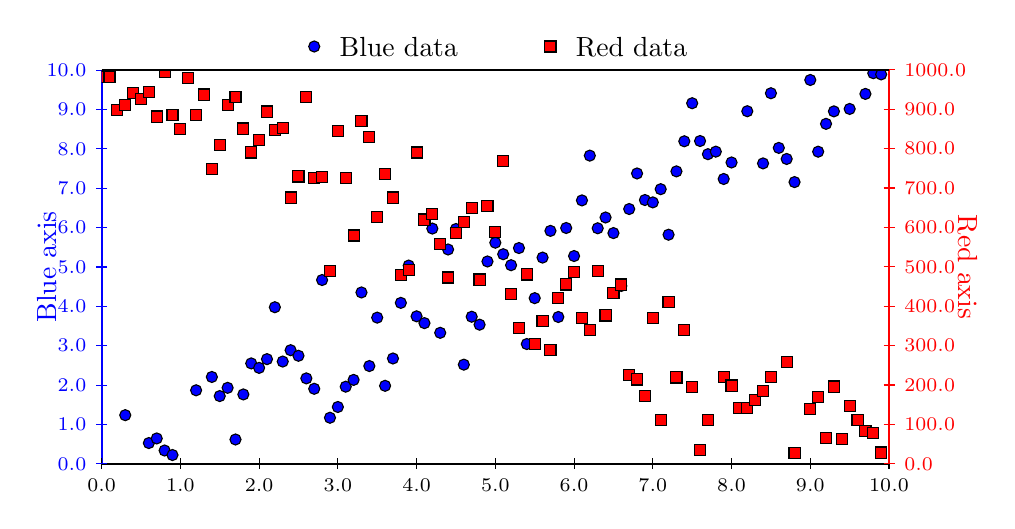
\begin{tikzpicture}
\draw[thick,black] (0.0,0.0) -- (10.0,0.0);
\draw[thick,blue] (0.0,0.0) -- (0.0,5.0);
\node[rotate=90,blue] at (-0.7,2.5) {Blue axis};
\begin{scope}[shift={(0.0,0.0)}]
\pgfsetxvec{\pgfpoint{1.0cm}{0cm}}
\pgfsetyvec{\pgfpoint{0cm}{0.5cm}}
\begin{scope}[shift={(0.0,0.0)}]
\begin{scope}[yshift=0cm]
\draw[black] [shift={(0.0,0.0)}] (0,2pt) -- (0,-2pt) node[below]{ \scriptsize{\num[round-mode=places,round-precision=1]{0}}};
\draw[black] [shift={(1.0,0.0)}] (0,2pt) -- (0,-2pt) node[below]{ \scriptsize{\num[round-mode=places,round-precision=1]{1}}};
\draw[black] [shift={(2.0,0.0)}] (0,2pt) -- (0,-2pt) node[below]{ \scriptsize{\num[round-mode=places,round-precision=1]{2}}};
\draw[black] [shift={(3.0,0.0)}] (0,2pt) -- (0,-2pt) node[below]{ \scriptsize{\num[round-mode=places,round-precision=1]{3}}};
\draw[black] [shift={(4.0,0.0)}] (0,2pt) -- (0,-2pt) node[below]{ \scriptsize{\num[round-mode=places,round-precision=1]{4}}};
\draw[black] [shift={(5.0,0.0)}] (0,2pt) -- (0,-2pt) node[below]{ \scriptsize{\num[round-mode=places,round-precision=1]{5}}};
\draw[black] [shift={(6.0,0.0)}] (0,2pt) -- (0,-2pt) node[below]{ \scriptsize{\num[round-mode=places,round-precision=1]{6}}};
\draw[black] [shift={(7.0,0.0)}] (0,2pt) -- (0,-2pt) node[below]{ \scriptsize{\num[round-mode=places,round-precision=1]{7}}};
\draw[black] [shift={(8.0,0.0)}] (0,2pt) -- (0,-2pt) node[below]{ \scriptsize{\num[round-mode=places,round-precision=1]{8}}};
\draw[black] [shift={(9.0,0.0)}] (0,2pt) -- (0,-2pt) node[below]{ \scriptsize{\num[round-mode=places,round-precision=1]{9}}};
\draw[black] [shift={(10.0,0.0)}] (0,2pt) -- (0,-2pt) node[below]{ \scriptsize{\num[round-mode=places,round-precision=1]{10}}};
\end{scope}
\begin{scope}[xshift=0cm]
\draw[blue] [shift={(0.0,0.0)}] (2pt,0) -- (-2pt,0) node[left]{ \scriptsize{\num[round-mode=places,round-precision=1]{0}}};
\draw[blue] [shift={(0.0,1.0)}] (2pt,0) -- (-2pt,0) node[left]{ \scriptsize{\num[round-mode=places,round-precision=1]{1}}};
\draw[blue] [shift={(0.0,2.0)}] (2pt,0) -- (-2pt,0) node[left]{ \scriptsize{\num[round-mode=places,round-precision=1]{2}}};
\draw[blue] [shift={(0.0,3.0)}] (2pt,0) -- (-2pt,0) node[left]{ \scriptsize{\num[round-mode=places,round-precision=1]{3}}};
\draw[blue] [shift={(0.0,4.0)}] (2pt,0) -- (-2pt,0) node[left]{ \scriptsize{\num[round-mode=places,round-precision=1]{4}}};
\draw[blue] [shift={(0.0,5.0)}] (2pt,0) -- (-2pt,0) node[left]{ \scriptsize{\num[round-mode=places,round-precision=1]{5}}};
\draw[blue] [shift={(0.0,6.0)}] (2pt,0) -- (-2pt,0) node[left]{ \scriptsize{\num[round-mode=places,round-precision=1]{6}}};
\draw[blue] [shift={(0.0,7.0)}] (2pt,0) -- (-2pt,0) node[left]{ \scriptsize{\num[round-mode=places,round-precision=1]{7}}};
\draw[blue] [shift={(0.0,8.0)}] (2pt,0) -- (-2pt,0) node[left]{ \scriptsize{\num[round-mode=places,round-precision=1]{8}}};
\draw[blue] [shift={(0.0,9.0)}] (2pt,0) -- (-2pt,0) node[left]{ \scriptsize{\num[round-mode=places,round-precision=1]{9}}};
\draw[blue] [shift={(0.0,10.0)}] (2pt,0) -- (-2pt,0) node[left]{ \scriptsize{\num[round-mode=places,round-precision=1]{10}}};
\end{scope}
\end{scope}
\pgfsetxvec{\pgfpoint{1cm}{0cm}}
\pgfsetyvec{\pgfpoint{0cm}{1cm}}
\end{scope}
\begin{scope}[]
\pgfpathmoveto{ \pgfpointxy {0.0} {0.0}}
\pgfpathlineto{ \pgfpointxy {10.0} {0.0}}
\pgfpathlineto{ \pgfpointxy {10.0} {5.0}}
\pgfpathlineto{ \pgfpointxy {0.0} {5.0}}
\pgfpathclose
\pgfusepath{  clip, }
\begin{scope}[shift={(0.0,0.0)}]
\pgfsetxvec{\pgfpoint{1.0cm}{0cm}}
\pgfsetyvec{\pgfpoint{0cm}{0.5cm}}
\begin{scope}[shift={(0.0,0.0)}]
\node at (0.0,-0.7530540812367451) [circle,inner sep=0.0pt,minimum width =4.0pt,minimum height=4.0pt,draw=black,fill=blue] {}; 
\node at (0.1,-0.19245240060567814) [circle,inner sep=0.0pt,minimum width =4.0pt,minimum height=4.0pt,draw=black,fill=blue] {}; 
\node at (0.2,-0.9948281282918419) [circle,inner sep=0.0pt,minimum width =4.0pt,minimum height=4.0pt,draw=black,fill=blue] {}; 
\node at (0.3,1.2360955245793792) [circle,inner sep=0.0pt,minimum width =4.0pt,minimum height=4.0pt,draw=black,fill=blue] {}; 
\node at (0.4,-0.7592752848197069) [circle,inner sep=0.0pt,minimum width =4.0pt,minimum height=4.0pt,draw=black,fill=blue] {}; 
\node at (0.5,-0.3378204509736439) [circle,inner sep=0.0pt,minimum width =4.0pt,minimum height=4.0pt,draw=black,fill=blue] {}; 
\node at (0.6,0.5280566481451047) [circle,inner sep=0.0pt,minimum width =4.0pt,minimum height=4.0pt,draw=black,fill=blue] {}; 
\node at (0.7,0.644847535636478) [circle,inner sep=0.0pt,minimum width =4.0pt,minimum height=4.0pt,draw=black,fill=blue] {}; 
\node at (0.8,0.3384206873539709) [circle,inner sep=0.0pt,minimum width =4.0pt,minimum height=4.0pt,draw=black,fill=blue] {}; 
\node at (0.90000004,0.2234748009420654) [circle,inner sep=0.0pt,minimum width =4.0pt,minimum height=4.0pt,draw=black,fill=blue] {}; 
\node at (1.0,-0.4681670196731367) [circle,inner sep=0.0pt,minimum width =4.0pt,minimum height=4.0pt,draw=black,fill=blue] {}; 
\node at (1.1,-1.1115272837278871) [circle,inner sep=0.0pt,minimum width =4.0pt,minimum height=4.0pt,draw=black,fill=blue] {}; 
\node at (1.2,1.8679282591678632) [circle,inner sep=0.0pt,minimum width =4.0pt,minimum height=4.0pt,draw=black,fill=blue] {}; 
\node at (1.3000001,-0.5884754757348241) [circle,inner sep=0.0pt,minimum width =4.0pt,minimum height=4.0pt,draw=black,fill=blue] {}; 
\node at (1.4,2.2062262374337958) [circle,inner sep=0.0pt,minimum width =4.0pt,minimum height=4.0pt,draw=black,fill=blue] {}; 
\node at (1.5,1.72083783095411) [circle,inner sep=0.0pt,minimum width =4.0pt,minimum height=4.0pt,draw=black,fill=blue] {}; 
\node at (1.6,1.9302354963776545) [circle,inner sep=0.0pt,minimum width =4.0pt,minimum height=4.0pt,draw=black,fill=blue] {}; 
\node at (1.7,0.618217960981688) [circle,inner sep=0.0pt,minimum width =4.0pt,minimum height=4.0pt,draw=black,fill=blue] {}; 
\node at (1.8000001,1.762848647073242) [circle,inner sep=0.0pt,minimum width =4.0pt,minimum height=4.0pt,draw=black,fill=blue] {}; 
\node at (1.9,2.5507362509575953) [circle,inner sep=0.0pt,minimum width =4.0pt,minimum height=4.0pt,draw=black,fill=blue] {}; 
\node at (2.0,2.437298058546523) [circle,inner sep=0.0pt,minimum width =4.0pt,minimum height=4.0pt,draw=black,fill=blue] {}; 
\node at (2.1000001,2.6588527165779468) [circle,inner sep=0.0pt,minimum width =4.0pt,minimum height=4.0pt,draw=black,fill=blue] {}; 
\node at (2.2,3.9777581964098223) [circle,inner sep=0.0pt,minimum width =4.0pt,minimum height=4.0pt,draw=black,fill=blue] {}; 
\node at (2.3,2.597885043074949) [circle,inner sep=0.0pt,minimum width =4.0pt,minimum height=4.0pt,draw=black,fill=blue] {}; 
\node at (2.4,2.886102140370506) [circle,inner sep=0.0pt,minimum width =4.0pt,minimum height=4.0pt,draw=black,fill=blue] {}; 
\node at (2.5,2.7445879656122583) [circle,inner sep=0.0pt,minimum width =4.0pt,minimum height=4.0pt,draw=black,fill=blue] {}; 
\node at (2.6000001,2.170424513257939) [circle,inner sep=0.0pt,minimum width =4.0pt,minimum height=4.0pt,draw=black,fill=blue] {}; 
\node at (2.7,1.9060715200574303) [circle,inner sep=0.0pt,minimum width =4.0pt,minimum height=4.0pt,draw=black,fill=blue] {}; 
\node at (2.8,4.668524182732347) [circle,inner sep=0.0pt,minimum width =4.0pt,minimum height=4.0pt,draw=black,fill=blue] {}; 
\node at (2.9,1.170447974326179) [circle,inner sep=0.0pt,minimum width =4.0pt,minimum height=4.0pt,draw=black,fill=blue] {}; 
\node at (3.0,1.4436195396750098) [circle,inner sep=0.0pt,minimum width =4.0pt,minimum height=4.0pt,draw=black,fill=blue] {}; 
\node at (3.1000001,1.9596133813722605) [circle,inner sep=0.0pt,minimum width =4.0pt,minimum height=4.0pt,draw=black,fill=blue] {}; 
\node at (3.2,2.1320164144779152) [circle,inner sep=0.0pt,minimum width =4.0pt,minimum height=4.0pt,draw=black,fill=blue] {}; 
\node at (3.3,4.353139532142527) [circle,inner sep=0.0pt,minimum width =4.0pt,minimum height=4.0pt,draw=black,fill=blue] {}; 
\node at (3.4,2.483811977863571) [circle,inner sep=0.0pt,minimum width =4.0pt,minimum height=4.0pt,draw=black,fill=blue] {}; 
\node at (3.5,3.7134310382244915) [circle,inner sep=0.0pt,minimum width =4.0pt,minimum height=4.0pt,draw=black,fill=blue] {}; 
\node at (3.6000001,1.981589507446402) [circle,inner sep=0.0pt,minimum width =4.0pt,minimum height=4.0pt,draw=black,fill=blue] {}; 
\node at (3.7,2.6758132617281634) [circle,inner sep=0.0pt,minimum width =4.0pt,minimum height=4.0pt,draw=black,fill=blue] {}; 
\node at (3.8,4.088017081897185) [circle,inner sep=0.0pt,minimum width =4.0pt,minimum height=4.0pt,draw=black,fill=blue] {}; 
\node at (3.9,5.03582606908318) [circle,inner sep=0.0pt,minimum width =4.0pt,minimum height=4.0pt,draw=black,fill=blue] {}; 
\node at (4.0,3.746582039322406) [circle,inner sep=0.0pt,minimum width =4.0pt,minimum height=4.0pt,draw=black,fill=blue] {}; 
\node at (4.1,3.57390630184206) [circle,inner sep=0.0pt,minimum width =4.0pt,minimum height=4.0pt,draw=black,fill=blue] {}; 
\node at (4.2000003,5.9759555044435375) [circle,inner sep=0.0pt,minimum width =4.0pt,minimum height=4.0pt,draw=black,fill=blue] {}; 
\node at (4.3,3.3277077561476602) [circle,inner sep=0.0pt,minimum width =4.0pt,minimum height=4.0pt,draw=black,fill=blue] {}; 
\node at (4.4,5.444054108524836) [circle,inner sep=0.0pt,minimum width =4.0pt,minimum height=4.0pt,draw=black,fill=blue] {}; 
\node at (4.5,5.964465608919078) [circle,inner sep=0.0pt,minimum width =4.0pt,minimum height=4.0pt,draw=black,fill=blue] {}; 
\node at (4.6,2.519294232475578) [circle,inner sep=0.0pt,minimum width =4.0pt,minimum height=4.0pt,draw=black,fill=blue] {}; 
\node at (4.7000003,3.7361120691586835) [circle,inner sep=0.0pt,minimum width =4.0pt,minimum height=4.0pt,draw=black,fill=blue] {}; 
\node at (4.8,3.534386801456381) [circle,inner sep=0.0pt,minimum width =4.0pt,minimum height=4.0pt,draw=black,fill=blue] {}; 
\node at (4.9,5.140002633549183) [circle,inner sep=0.0pt,minimum width =4.0pt,minimum height=4.0pt,draw=black,fill=blue] {}; 
\node at (5.0,5.616607534185556) [circle,inner sep=0.0pt,minimum width =4.0pt,minimum height=4.0pt,draw=black,fill=blue] {}; 
\node at (5.1,5.324377172179913) [circle,inner sep=0.0pt,minimum width =4.0pt,minimum height=4.0pt,draw=black,fill=blue] {}; 
\node at (5.2000003,5.045145716668884) [circle,inner sep=0.0pt,minimum width =4.0pt,minimum height=4.0pt,draw=black,fill=blue] {}; 
\node at (5.3,5.480760356887337) [circle,inner sep=0.0pt,minimum width =4.0pt,minimum height=4.0pt,draw=black,fill=blue] {}; 
\node at (5.4,3.0429712564331424) [circle,inner sep=0.0pt,minimum width =4.0pt,minimum height=4.0pt,draw=black,fill=blue] {}; 
\node at (5.5,4.208123475592149) [circle,inner sep=0.0pt,minimum width =4.0pt,minimum height=4.0pt,draw=black,fill=blue] {}; 
\node at (5.6,5.238246904678464) [circle,inner sep=0.0pt,minimum width =4.0pt,minimum height=4.0pt,draw=black,fill=blue] {}; 
\node at (5.7000003,5.916901394532718) [circle,inner sep=0.0pt,minimum width =4.0pt,minimum height=4.0pt,draw=black,fill=blue] {}; 
\node at (5.8,3.729491705327055) [circle,inner sep=0.0pt,minimum width =4.0pt,minimum height=4.0pt,draw=black,fill=blue] {}; 
\node at (5.9,5.990126386362027) [circle,inner sep=0.0pt,minimum width =4.0pt,minimum height=4.0pt,draw=black,fill=blue] {}; 
\node at (6.0,5.277921215283762) [circle,inner sep=0.0pt,minimum width =4.0pt,minimum height=4.0pt,draw=black,fill=blue] {}; 
\node at (6.1,6.690964647108347) [circle,inner sep=0.0pt,minimum width =4.0pt,minimum height=4.0pt,draw=black,fill=blue] {}; 
\node at (6.2000003,7.828442138923822) [circle,inner sep=0.0pt,minimum width =4.0pt,minimum height=4.0pt,draw=black,fill=blue] {}; 
\node at (6.3,5.983121763554156) [circle,inner sep=0.0pt,minimum width =4.0pt,minimum height=4.0pt,draw=black,fill=blue] {}; 
\node at (6.4,6.257124651021646) [circle,inner sep=0.0pt,minimum width =4.0pt,minimum height=4.0pt,draw=black,fill=blue] {}; 
\node at (6.5,5.860624599438689) [circle,inner sep=0.0pt,minimum width =4.0pt,minimum height=4.0pt,draw=black,fill=blue] {}; 
\node at (6.6,4.518958518741558) [circle,inner sep=0.0pt,minimum width =4.0pt,minimum height=4.0pt,draw=black,fill=blue] {}; 
\node at (6.7000003,6.47177219558856) [circle,inner sep=0.0pt,minimum width =4.0pt,minimum height=4.0pt,draw=black,fill=blue] {}; 
\node at (6.8,7.375343300127703) [circle,inner sep=0.0pt,minimum width =4.0pt,minimum height=4.0pt,draw=black,fill=blue] {}; 
\node at (6.9,6.700974459260845) [circle,inner sep=0.0pt,minimum width =4.0pt,minimum height=4.0pt,draw=black,fill=blue] {}; 
\node at (7.0,6.6405588307941805) [circle,inner sep=0.0pt,minimum width =4.0pt,minimum height=4.0pt,draw=black,fill=blue] {}; 
\node at (7.1,6.975973735181482) [circle,inner sep=0.0pt,minimum width =4.0pt,minimum height=4.0pt,draw=black,fill=blue] {}; 
\node at (7.2000003,5.819641796197111) [circle,inner sep=0.0pt,minimum width =4.0pt,minimum height=4.0pt,draw=black,fill=blue] {}; 
\node at (7.3,7.4283683792421) [circle,inner sep=0.0pt,minimum width =4.0pt,minimum height=4.0pt,draw=black,fill=blue] {}; 
\node at (7.4,8.192575500264487) [circle,inner sep=0.0pt,minimum width =4.0pt,minimum height=4.0pt,draw=black,fill=blue] {}; 
\node at (7.5,9.159286969624922) [circle,inner sep=0.0pt,minimum width =4.0pt,minimum height=4.0pt,draw=black,fill=blue] {}; 
\node at (7.6,8.199303985102667) [circle,inner sep=0.0pt,minimum width =4.0pt,minimum height=4.0pt,draw=black,fill=blue] {}; 
\node at (7.7000003,7.864938970529522) [circle,inner sep=0.0pt,minimum width =4.0pt,minimum height=4.0pt,draw=black,fill=blue] {}; 
\node at (7.8,7.929455827171371) [circle,inner sep=0.0pt,minimum width =4.0pt,minimum height=4.0pt,draw=black,fill=blue] {}; 
\node at (7.9,7.235015454141253) [circle,inner sep=0.0pt,minimum width =4.0pt,minimum height=4.0pt,draw=black,fill=blue] {}; 
\node at (8.0,7.654345497372451) [circle,inner sep=0.0pt,minimum width =4.0pt,minimum height=4.0pt,draw=black,fill=blue] {}; 
\node at (8.1,10.568074022150892) [circle,inner sep=0.0pt,minimum width =4.0pt,minimum height=4.0pt,draw=black,fill=blue] {}; 
\node at (8.2,8.956128574505636) [circle,inner sep=0.0pt,minimum width =4.0pt,minimum height=4.0pt,draw=black,fill=blue] {}; 
\node at (8.3,10.311361478202741) [circle,inner sep=0.0pt,minimum width =4.0pt,minimum height=4.0pt,draw=black,fill=blue] {}; 
\node at (8.400001,7.630942819092076) [circle,inner sep=0.0pt,minimum width =4.0pt,minimum height=4.0pt,draw=black,fill=blue] {}; 
\node at (8.5,9.412956452412532) [circle,inner sep=0.0pt,minimum width =4.0pt,minimum height=4.0pt,draw=black,fill=blue] {}; 
\node at (8.6,8.024640839202988) [circle,inner sep=0.0pt,minimum width =4.0pt,minimum height=4.0pt,draw=black,fill=blue] {}; 
\node at (8.7,7.743335604280339) [circle,inner sep=0.0pt,minimum width =4.0pt,minimum height=4.0pt,draw=black,fill=blue] {}; 
\node at (8.8,7.155941678401322) [circle,inner sep=0.0pt,minimum width =4.0pt,minimum height=4.0pt,draw=black,fill=blue] {}; 
\node at (8.900001,10.341656129517826) [circle,inner sep=0.0pt,minimum width =4.0pt,minimum height=4.0pt,draw=black,fill=blue] {}; 
\node at (9.0,9.749648035151543) [circle,inner sep=0.0pt,minimum width =4.0pt,minimum height=4.0pt,draw=black,fill=blue] {}; 
\node at (9.1,7.928233850475681) [circle,inner sep=0.0pt,minimum width =4.0pt,minimum height=4.0pt,draw=black,fill=blue] {}; 
\node at (9.2,8.63541989439423) [circle,inner sep=0.0pt,minimum width =4.0pt,minimum height=4.0pt,draw=black,fill=blue] {}; 
\node at (9.3,8.952267726498674) [circle,inner sep=0.0pt,minimum width =4.0pt,minimum height=4.0pt,draw=black,fill=blue] {}; 
\node at (9.400001,11.679149481388594) [circle,inner sep=0.0pt,minimum width =4.0pt,minimum height=4.0pt,draw=black,fill=blue] {}; 
\node at (9.5,9.013953895369418) [circle,inner sep=0.0pt,minimum width =4.0pt,minimum height=4.0pt,draw=black,fill=blue] {}; 
\node at (9.6,10.170004549041604) [circle,inner sep=0.0pt,minimum width =4.0pt,minimum height=4.0pt,draw=black,fill=blue] {}; 
\node at (9.7,9.396127566279688) [circle,inner sep=0.0pt,minimum width =4.0pt,minimum height=4.0pt,draw=black,fill=blue] {}; 
\node at (9.8,9.922220561459543) [circle,inner sep=0.0pt,minimum width =4.0pt,minimum height=4.0pt,draw=black,fill=blue] {}; 
\node at (9.900001,9.891468919532596) [circle,inner sep=0.0pt,minimum width =4.0pt,minimum height=4.0pt,draw=black,fill=blue] {}; 
\node at (10.0,12.019643641089365) [circle,inner sep=0.0pt,minimum width =4.0pt,minimum height=4.0pt,draw=black,fill=blue] {}; 
\end{scope}
\pgfsetxvec{\pgfpoint{1cm}{0cm}}
\pgfsetyvec{\pgfpoint{0cm}{1cm}}
\end{scope}
\end{scope}
\draw[thick,red] (10.0,0.0) -- (10.0,5.0);
\node[rotate=-90,red] at (11.0,2.5) {Red axis};
\begin{scope}[shift={(0.0,0.0)}]
\pgfsetxvec{\pgfpoint{1.0cm}{0cm}}
\pgfsetyvec{\pgfpoint{0cm}{0.005cm}}
\begin{scope}[shift={(0.0,0.0)}]
\begin{scope}[xshift=10cm]
\draw[red] [shift={(0.0,0.0)}] (-2pt,0) -- (2pt,0) node[right]{ \scriptsize{\num[round-mode=places,round-precision=1]{0}}};
\draw[red] [shift={(0.0,100.0)}] (-2pt,0) -- (2pt,0) node[right]{ \scriptsize{\num[round-mode=places,round-precision=1]{100}}};
\draw[red] [shift={(0.0,200.0)}] (-2pt,0) -- (2pt,0) node[right]{ \scriptsize{\num[round-mode=places,round-precision=1]{200}}};
\draw[red] [shift={(0.0,300.0)}] (-2pt,0) -- (2pt,0) node[right]{ \scriptsize{\num[round-mode=places,round-precision=1]{300}}};
\draw[red] [shift={(0.0,400.0)}] (-2pt,0) -- (2pt,0) node[right]{ \scriptsize{\num[round-mode=places,round-precision=1]{400}}};
\draw[red] [shift={(0.0,500.0)}] (-2pt,0) -- (2pt,0) node[right]{ \scriptsize{\num[round-mode=places,round-precision=1]{500}}};
\draw[red] [shift={(0.0,600.0)}] (-2pt,0) -- (2pt,0) node[right]{ \scriptsize{\num[round-mode=places,round-precision=1]{600}}};
\draw[red] [shift={(0.0,700.0)}] (-2pt,0) -- (2pt,0) node[right]{ \scriptsize{\num[round-mode=places,round-precision=1]{700}}};
\draw[red] [shift={(0.0,800.0)}] (-2pt,0) -- (2pt,0) node[right]{ \scriptsize{\num[round-mode=places,round-precision=1]{800}}};
\draw[red] [shift={(0.0,900.0)}] (-2pt,0) -- (2pt,0) node[right]{ \scriptsize{\num[round-mode=places,round-precision=1]{900}}};
\draw[red] [shift={(0.0,1000.0)}] (-2pt,0) -- (2pt,0) node[right]{ \scriptsize{\num[round-mode=places,round-precision=1]{1000}}};
\end{scope}
\end{scope}
\pgfsetxvec{\pgfpoint{1cm}{0cm}}
\pgfsetyvec{\pgfpoint{0cm}{1cm}}
\end{scope}
\begin{scope}[]
\pgfpathmoveto{ \pgfpointxy {0.0} {0.0}}
\pgfpathlineto{ \pgfpointxy {10.0} {0.0}}
\pgfpathlineto{ \pgfpointxy {10.0} {5.0}}
\pgfpathlineto{ \pgfpointxy {0.0} {5.0}}
\pgfpathclose
\pgfusepath{  clip, }
\begin{scope}[shift={(0.0,0.0)}]
\pgfsetxvec{\pgfpoint{1.0cm}{0cm}}
\pgfsetyvec{\pgfpoint{0cm}{0.005cm}}
\begin{scope}[shift={(0.0,0.0)}]
\node at (0.0,982.8389594478306) [rectangle,inner sep=0.0pt,minimum width =4.0pt,minimum height=4.0pt,draw=black,fill=red] {}; 
\node at (0.1,982.1179277735966) [rectangle,inner sep=0.0pt,minimum width =4.0pt,minimum height=4.0pt,draw=black,fill=red] {}; 
\node at (0.2,898.8058813446663) [rectangle,inner sep=0.0pt,minimum width =4.0pt,minimum height=4.0pt,draw=black,fill=red] {}; 
\node at (0.3,910.3599663621553) [rectangle,inner sep=0.0pt,minimum width =4.0pt,minimum height=4.0pt,draw=black,fill=red] {}; 
\node at (0.4,941.5981237958409) [rectangle,inner sep=0.0pt,minimum width =4.0pt,minimum height=4.0pt,draw=black,fill=red] {}; 
\node at (0.5,925.5686276745464) [rectangle,inner sep=0.0pt,minimum width =4.0pt,minimum height=4.0pt,draw=black,fill=red] {}; 
\node at (0.6,943.0437744669227) [rectangle,inner sep=0.0pt,minimum width =4.0pt,minimum height=4.0pt,draw=black,fill=red] {}; 
\node at (0.7,881.3214483270589) [rectangle,inner sep=0.0pt,minimum width =4.0pt,minimum height=4.0pt,draw=black,fill=red] {}; 
\node at (0.8,994.4914550345453) [rectangle,inner sep=0.0pt,minimum width =4.0pt,minimum height=4.0pt,draw=black,fill=red] {}; 
\node at (0.90000004,885.302120750967) [rectangle,inner sep=0.0pt,minimum width =4.0pt,minimum height=4.0pt,draw=black,fill=red] {}; 
\node at (1.0,849.3347794799167) [rectangle,inner sep=0.0pt,minimum width =4.0pt,minimum height=4.0pt,draw=black,fill=red] {}; 
\node at (1.1,979.5069715731291) [rectangle,inner sep=0.0pt,minimum width =4.0pt,minimum height=4.0pt,draw=black,fill=red] {}; 
\node at (1.2,885.0722579198873) [rectangle,inner sep=0.0pt,minimum width =4.0pt,minimum height=4.0pt,draw=black,fill=red] {}; 
\node at (1.3000001,937.1188052180031) [rectangle,inner sep=0.0pt,minimum width =4.0pt,minimum height=4.0pt,draw=black,fill=red] {}; 
\node at (1.4,747.2997249086955) [rectangle,inner sep=0.0pt,minimum width =4.0pt,minimum height=4.0pt,draw=black,fill=red] {}; 
\node at (1.5,809.0604014661525) [rectangle,inner sep=0.0pt,minimum width =4.0pt,minimum height=4.0pt,draw=black,fill=red] {}; 
\node at (1.6,911.4872080037733) [rectangle,inner sep=0.0pt,minimum width =4.0pt,minimum height=4.0pt,draw=black,fill=red] {}; 
\node at (1.7,931.0178977052036) [rectangle,inner sep=0.0pt,minimum width =4.0pt,minimum height=4.0pt,draw=black,fill=red] {}; 
\node at (1.8000001,850.8139479844182) [rectangle,inner sep=0.0pt,minimum width =4.0pt,minimum height=4.0pt,draw=black,fill=red] {}; 
\node at (1.9,790.1129846160436) [rectangle,inner sep=0.0pt,minimum width =4.0pt,minimum height=4.0pt,draw=black,fill=red] {}; 
\node at (2.0,822.2373586315096) [rectangle,inner sep=0.0pt,minimum width =4.0pt,minimum height=4.0pt,draw=black,fill=red] {}; 
\node at (2.1000001,893.85630155428) [rectangle,inner sep=0.0pt,minimum width =4.0pt,minimum height=4.0pt,draw=black,fill=red] {}; 
\node at (2.2,846.2321477573038) [rectangle,inner sep=0.0pt,minimum width =4.0pt,minimum height=4.0pt,draw=black,fill=red] {}; 
\node at (2.3,852.9149036329613) [rectangle,inner sep=0.0pt,minimum width =4.0pt,minimum height=4.0pt,draw=black,fill=red] {}; 
\node at (2.4,675.6733649976662) [rectangle,inner sep=0.0pt,minimum width =4.0pt,minimum height=4.0pt,draw=black,fill=red] {}; 
\node at (2.5,729.2951250260766) [rectangle,inner sep=0.0pt,minimum width =4.0pt,minimum height=4.0pt,draw=black,fill=red] {}; 
\node at (2.6000001,931.6822599859977) [rectangle,inner sep=0.0pt,minimum width =4.0pt,minimum height=4.0pt,draw=black,fill=red] {}; 
\node at (2.7,725.9302427777089) [rectangle,inner sep=0.0pt,minimum width =4.0pt,minimum height=4.0pt,draw=black,fill=red] {}; 
\node at (2.8,728.4096774706213) [rectangle,inner sep=0.0pt,minimum width =4.0pt,minimum height=4.0pt,draw=black,fill=red] {}; 
\node at (2.9,490.203423084229) [rectangle,inner sep=0.0pt,minimum width =4.0pt,minimum height=4.0pt,draw=black,fill=red] {}; 
\node at (3.0,844.6296204658106) [rectangle,inner sep=0.0pt,minimum width =4.0pt,minimum height=4.0pt,draw=black,fill=red] {}; 
\node at (3.1000001,724.5241130788975) [rectangle,inner sep=0.0pt,minimum width =4.0pt,minimum height=4.0pt,draw=black,fill=red] {}; 
\node at (3.2,579.4043272515684) [rectangle,inner sep=0.0pt,minimum width =4.0pt,minimum height=4.0pt,draw=black,fill=red] {}; 
\node at (3.3,870.2416276164889) [rectangle,inner sep=0.0pt,minimum width =4.0pt,minimum height=4.0pt,draw=black,fill=red] {}; 
\node at (3.4,829.2231355632032) [rectangle,inner sep=0.0pt,minimum width =4.0pt,minimum height=4.0pt,draw=black,fill=red] {}; 
\node at (3.5,626.7279957100719) [rectangle,inner sep=0.0pt,minimum width =4.0pt,minimum height=4.0pt,draw=black,fill=red] {}; 
\node at (3.6000001,736.3593826429662) [rectangle,inner sep=0.0pt,minimum width =4.0pt,minimum height=4.0pt,draw=black,fill=red] {}; 
\node at (3.7,675.7204025729593) [rectangle,inner sep=0.0pt,minimum width =4.0pt,minimum height=4.0pt,draw=black,fill=red] {}; 
\node at (3.8,478.49651753774083) [rectangle,inner sep=0.0pt,minimum width =4.0pt,minimum height=4.0pt,draw=black,fill=red] {}; 
\node at (3.9,492.7944352327862) [rectangle,inner sep=0.0pt,minimum width =4.0pt,minimum height=4.0pt,draw=black,fill=red] {}; 
\node at (4.0,790.0175620675691) [rectangle,inner sep=0.0pt,minimum width =4.0pt,minimum height=4.0pt,draw=black,fill=red] {}; 
\node at (4.1,619.7893753324179) [rectangle,inner sep=0.0pt,minimum width =4.0pt,minimum height=4.0pt,draw=black,fill=red] {}; 
\node at (4.2000003,634.5816817486708) [rectangle,inner sep=0.0pt,minimum width =4.0pt,minimum height=4.0pt,draw=black,fill=red] {}; 
\node at (4.3,557.3025045631995) [rectangle,inner sep=0.0pt,minimum width =4.0pt,minimum height=4.0pt,draw=black,fill=red] {}; 
\node at (4.4,472.8170650429166) [rectangle,inner sep=0.0pt,minimum width =4.0pt,minimum height=4.0pt,draw=black,fill=red] {}; 
\node at (4.5,585.7730564768681) [rectangle,inner sep=0.0pt,minimum width =4.0pt,minimum height=4.0pt,draw=black,fill=red] {}; 
\node at (4.6,613.0367867572984) [rectangle,inner sep=0.0pt,minimum width =4.0pt,minimum height=4.0pt,draw=black,fill=red] {}; 
\node at (4.7000003,648.8644386868501) [rectangle,inner sep=0.0pt,minimum width =4.0pt,minimum height=4.0pt,draw=black,fill=red] {}; 
\node at (4.8,467.64922302803365) [rectangle,inner sep=0.0pt,minimum width =4.0pt,minimum height=4.0pt,draw=black,fill=red] {}; 
\node at (4.9,654.8127851688978) [rectangle,inner sep=0.0pt,minimum width =4.0pt,minimum height=4.0pt,draw=black,fill=red] {}; 
\node at (5.0,587.9220658476062) [rectangle,inner sep=0.0pt,minimum width =4.0pt,minimum height=4.0pt,draw=black,fill=red] {}; 
\node at (5.1,767.5048349393091) [rectangle,inner sep=0.0pt,minimum width =4.0pt,minimum height=4.0pt,draw=black,fill=red] {}; 
\node at (5.2000003,430.7553991072592) [rectangle,inner sep=0.0pt,minimum width =4.0pt,minimum height=4.0pt,draw=black,fill=red] {}; 
\node at (5.3,343.65528516979583) [rectangle,inner sep=0.0pt,minimum width =4.0pt,minimum height=4.0pt,draw=black,fill=red] {}; 
\node at (5.4,480.60179060754234) [rectangle,inner sep=0.0pt,minimum width =4.0pt,minimum height=4.0pt,draw=black,fill=red] {}; 
\node at (5.5,304.22715507889376) [rectangle,inner sep=0.0pt,minimum width =4.0pt,minimum height=4.0pt,draw=black,fill=red] {}; 
\node at (5.6,361.598874554722) [rectangle,inner sep=0.0pt,minimum width =4.0pt,minimum height=4.0pt,draw=black,fill=red] {}; 
\node at (5.7000003,288.38085417554413) [rectangle,inner sep=0.0pt,minimum width =4.0pt,minimum height=4.0pt,draw=black,fill=red] {}; 
\node at (5.8,421.55540560497514) [rectangle,inner sep=0.0pt,minimum width =4.0pt,minimum height=4.0pt,draw=black,fill=red] {}; 
\node at (5.9,455.20066086127366) [rectangle,inner sep=0.0pt,minimum width =4.0pt,minimum height=4.0pt,draw=black,fill=red] {}; 
\node at (6.0,486.04111773348) [rectangle,inner sep=0.0pt,minimum width =4.0pt,minimum height=4.0pt,draw=black,fill=red] {}; 
\node at (6.1,370.0399120257215) [rectangle,inner sep=0.0pt,minimum width =4.0pt,minimum height=4.0pt,draw=black,fill=red] {}; 
\node at (6.2000003,340.14302253862303) [rectangle,inner sep=0.0pt,minimum width =4.0pt,minimum height=4.0pt,draw=black,fill=red] {}; 
\node at (6.3,490.3471411739477) [rectangle,inner sep=0.0pt,minimum width =4.0pt,minimum height=4.0pt,draw=black,fill=red] {}; 
\node at (6.4,376.58953505404077) [rectangle,inner sep=0.0pt,minimum width =4.0pt,minimum height=4.0pt,draw=black,fill=red] {}; 
\node at (6.5,433.8206891358261) [rectangle,inner sep=0.0pt,minimum width =4.0pt,minimum height=4.0pt,draw=black,fill=red] {}; 
\node at (6.6,454.9512725298192) [rectangle,inner sep=0.0pt,minimum width =4.0pt,minimum height=4.0pt,draw=black,fill=red] {}; 
\node at (6.7000003,224.75310336823247) [rectangle,inner sep=0.0pt,minimum width =4.0pt,minimum height=4.0pt,draw=black,fill=red] {}; 
\node at (6.8,214.05721054918772) [rectangle,inner sep=0.0pt,minimum width =4.0pt,minimum height=4.0pt,draw=black,fill=red] {}; 
\node at (6.9,172.52492754585978) [rectangle,inner sep=0.0pt,minimum width =4.0pt,minimum height=4.0pt,draw=black,fill=red] {}; 
\node at (7.0,369.5344396316222) [rectangle,inner sep=0.0pt,minimum width =4.0pt,minimum height=4.0pt,draw=black,fill=red] {}; 
\node at (7.1,111.97429344542478) [rectangle,inner sep=0.0pt,minimum width =4.0pt,minimum height=4.0pt,draw=black,fill=red] {}; 
\node at (7.2000003,411.5818929838782) [rectangle,inner sep=0.0pt,minimum width =4.0pt,minimum height=4.0pt,draw=black,fill=red] {}; 
\node at (7.3,219.1741430102498) [rectangle,inner sep=0.0pt,minimum width =4.0pt,minimum height=4.0pt,draw=black,fill=red] {}; 
\node at (7.4,339.06099207989274) [rectangle,inner sep=0.0pt,minimum width =4.0pt,minimum height=4.0pt,draw=black,fill=red] {}; 
\node at (7.5,195.2863053566027) [rectangle,inner sep=0.0pt,minimum width =4.0pt,minimum height=4.0pt,draw=black,fill=red] {}; 
\node at (7.6,34.6712318423954) [rectangle,inner sep=0.0pt,minimum width =4.0pt,minimum height=4.0pt,draw=black,fill=red] {}; 
\node at (7.7000003,111.38565718459752) [rectangle,inner sep=0.0pt,minimum width =4.0pt,minimum height=4.0pt,draw=black,fill=red] {}; 
\node at (7.8,-65.8550723708025) [rectangle,inner sep=0.0pt,minimum width =4.0pt,minimum height=4.0pt,draw=black,fill=red] {}; 
\node at (7.9,221.0810365481155) [rectangle,inner sep=0.0pt,minimum width =4.0pt,minimum height=4.0pt,draw=black,fill=red] {}; 
\node at (8.0,198.6682596108775) [rectangle,inner sep=0.0pt,minimum width =4.0pt,minimum height=4.0pt,draw=black,fill=red] {}; 
\node at (8.1,141.4897073604376) [rectangle,inner sep=0.0pt,minimum width =4.0pt,minimum height=4.0pt,draw=black,fill=red] {}; 
\node at (8.2,141.62720772478502) [rectangle,inner sep=0.0pt,minimum width =4.0pt,minimum height=4.0pt,draw=black,fill=red] {}; 
\node at (8.3,161.2295796604995) [rectangle,inner sep=0.0pt,minimum width =4.0pt,minimum height=4.0pt,draw=black,fill=red] {}; 
\node at (8.400001,184.87792347055586) [rectangle,inner sep=0.0pt,minimum width =4.0pt,minimum height=4.0pt,draw=black,fill=red] {}; 
\node at (8.5,220.7674215683552) [rectangle,inner sep=0.0pt,minimum width =4.0pt,minimum height=4.0pt,draw=black,fill=red] {}; 
\node at (8.6,-49.075392373823234) [rectangle,inner sep=0.0pt,minimum width =4.0pt,minimum height=4.0pt,draw=black,fill=red] {}; 
\node at (8.7,258.25779048709927) [rectangle,inner sep=0.0pt,minimum width =4.0pt,minimum height=4.0pt,draw=black,fill=red] {}; 
\node at (8.8,26.808485678787797) [rectangle,inner sep=0.0pt,minimum width =4.0pt,minimum height=4.0pt,draw=black,fill=red] {}; 
\node at (8.900001,-19.0481540724301) [rectangle,inner sep=0.0pt,minimum width =4.0pt,minimum height=4.0pt,draw=black,fill=red] {}; 
\node at (9.0,138.5535211278233) [rectangle,inner sep=0.0pt,minimum width =4.0pt,minimum height=4.0pt,draw=black,fill=red] {}; 
\node at (9.1,169.4540514787434) [rectangle,inner sep=0.0pt,minimum width =4.0pt,minimum height=4.0pt,draw=black,fill=red] {}; 
\node at (9.2,64.99166224838876) [rectangle,inner sep=0.0pt,minimum width =4.0pt,minimum height=4.0pt,draw=black,fill=red] {}; 
\node at (9.3,196.03645564097116) [rectangle,inner sep=0.0pt,minimum width =4.0pt,minimum height=4.0pt,draw=black,fill=red] {}; 
\node at (9.400001,63.298429245649146) [rectangle,inner sep=0.0pt,minimum width =4.0pt,minimum height=4.0pt,draw=black,fill=red] {}; 
\node at (9.5,147.73341710900993) [rectangle,inner sep=0.0pt,minimum width =4.0pt,minimum height=4.0pt,draw=black,fill=red] {}; 
\node at (9.6,112.00827933614477) [rectangle,inner sep=0.0pt,minimum width =4.0pt,minimum height=4.0pt,draw=black,fill=red] {}; 
\node at (9.7,82.92013389062696) [rectangle,inner sep=0.0pt,minimum width =4.0pt,minimum height=4.0pt,draw=black,fill=red] {}; 
\node at (9.8,78.30874121057576) [rectangle,inner sep=0.0pt,minimum width =4.0pt,minimum height=4.0pt,draw=black,fill=red] {}; 
\node at (9.900001,28.609364691289052) [rectangle,inner sep=0.0pt,minimum width =4.0pt,minimum height=4.0pt,draw=black,fill=red] {}; 
\node at (10.0,-201.95819855233682) [rectangle,inner sep=0.0pt,minimum width =4.0pt,minimum height=4.0pt,draw=black,fill=red] {}; 
\end{scope}
\pgfsetxvec{\pgfpoint{1cm}{0cm}}
\pgfsetyvec{\pgfpoint{0cm}{1cm}}
\end{scope}
\end{scope}
\draw[thick,black] (0.0,5.0) -- (10.0,5.0);
\node at (5.7,5.3) [rectangle,inner sep=0.0pt,minimum width =4.0pt,minimum height=4.0pt,fill=red,draw=black] {}; 
\node[right,] at (5.9,5.3) {Red data};
\node at (2.7,5.3) [circle,inner sep=0.0pt,minimum width =4.0pt,minimum height=4.0pt,fill=blue,draw=black] {}; 
\node[right,] at (2.9,5.3) {Blue data};
\end{tikzpicture}
\end{document}

\captionsetup{singlelinecheck=off}
\caption[asdf]{Two data sets with different transformations are plotted on top of ech other.}
\end{figure}
\begin{figure}[H]
\centering
%%% AUTO GENERATED CODE
\documentclass{standalone}
\ifx\HCode\UnDef\else\def\pgfsysdriver{pgfsys-tex4ht.def}\fi
\usepackage[usenames,dvipsnames,svgnames,table]{xcolor}
\usepackage[utf8]{inputenc}
\usepackage[]{textcomp}
\usepackage{tikz}
\usepackage{color}
\usepackage{siunitx}
\usetikzlibrary{arrows,shapes}
\usetikzlibrary{decorations.markings}
\begin{document}
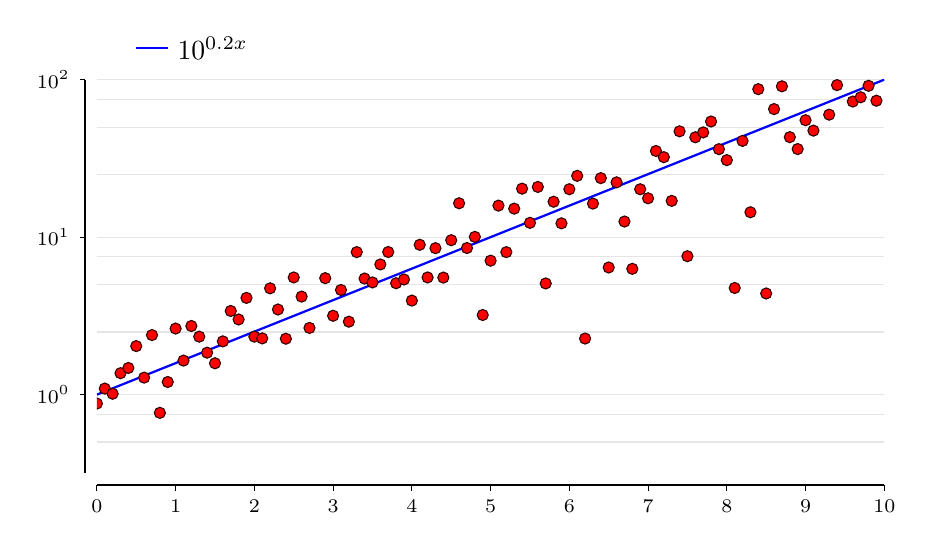
\begin{tikzpicture}[]
\begin{scope}[shift={(0.0,0.0)}]
\pgfsetxvec{\pgfpoint{1.0cm}{0cm}}
\pgfsetyvec{\pgfpoint{0cm}{2.0cm}}
\begin{scope}[shift={(0.0,0.5)}]
\begin{scope}[thick,black,fill=white]
\pgfpathmoveto{ \pgfpointadd{\pgfpointxy {0.0} {-0.5}} {\pgfpoint{0}{-0.15cm}} }
\pgfpathlineto{ \pgfpointadd{\pgfpointxy {10.0} {-0.5}} {\pgfpoint{0}{-0.15cm}} }
\pgfpathmoveto{ \pgfpointadd{\pgfpointxy {0.0} {-0.5}} {\pgfpoint{-0.15cm}{0}} }
\pgfpathlineto{ \pgfpointadd{\pgfpointxy {0.0} {2.0}} {\pgfpoint{-0.15cm}{0}} }
\pgfusepath{ stroke, }
\end{scope}
\begin{scope}[yshift=-0.15cm]
\draw[] [shift={(0.0,-0.5)}] (0,0) -- (0,-2pt) node[below]{ \scriptsize{\num[round-mode=places,round-precision=0]{0.0}}};
\draw[] [shift={(1.0,-0.5)}] (0,0) -- (0,-2pt) node[below]{ \scriptsize{\num[round-mode=places,round-precision=0]{1.0}}};
\draw[] [shift={(2.0,-0.5)}] (0,0) -- (0,-2pt) node[below]{ \scriptsize{\num[round-mode=places,round-precision=0]{2.0}}};
\draw[] [shift={(3.0,-0.5)}] (0,0) -- (0,-2pt) node[below]{ \scriptsize{\num[round-mode=places,round-precision=0]{3.0}}};
\draw[] [shift={(4.0,-0.5)}] (0,0) -- (0,-2pt) node[below]{ \scriptsize{\num[round-mode=places,round-precision=0]{4.0}}};
\draw[] [shift={(5.0,-0.5)}] (0,0) -- (0,-2pt) node[below]{ \scriptsize{\num[round-mode=places,round-precision=0]{5.0}}};
\draw[] [shift={(6.0,-0.5)}] (0,0) -- (0,-2pt) node[below]{ \scriptsize{\num[round-mode=places,round-precision=0]{6.0}}};
\draw[] [shift={(7.0,-0.5)}] (0,0) -- (0,-2pt) node[below]{ \scriptsize{\num[round-mode=places,round-precision=0]{7.0}}};
\draw[] [shift={(8.0,-0.5)}] (0,0) -- (0,-2pt) node[below]{ \scriptsize{\num[round-mode=places,round-precision=0]{8.0}}};
\draw[] [shift={(9.0,-0.5)}] (0,0) -- (0,-2pt) node[below]{ \scriptsize{\num[round-mode=places,round-precision=0]{9.0}}};
\draw[] [shift={(10.0,-0.5)}] (0,0) -- (0,-2pt) node[below]{ \scriptsize{\num[round-mode=places,round-precision=0]{10.0}}};
\end{scope}
\begin{scope}[xshift=-0.15cm]
\end{scope}
\end{scope}
\end{scope}
\pgfsetxvec{\pgfpoint{1cm}{0cm}}
\pgfsetyvec{\pgfpoint{0cm}{1cm}}
\begin{scope}[shift={(0.0,0.0)}]
\pgfsetxvec{\pgfpoint{1.0cm}{0cm}}
\pgfsetyvec{\pgfpoint{0cm}{2.0cm}}
\begin{scope}[shift={(0.0,0.5)}]
\begin{scope}[thin,gray!20!white]
\pgfpathmoveto{ \pgfpointxy {0.0} {-0.30102999566398114}}
\pgfpathlineto{ \pgfpointxy {10.0} {-0.30102999566398114}}
\pgfpathmoveto{ \pgfpointxy {0.0} {-0.12493873660829995}}
\pgfpathlineto{ \pgfpointxy {10.0} {-0.12493873660829995}}
\pgfpathmoveto{ \pgfpointxy {0.0} {0.0}}
\pgfpathlineto{ \pgfpointxy {10.0} {0.0}}
\pgfpathmoveto{ \pgfpointxy {0.0} {0.3979400086720376}}
\pgfpathlineto{ \pgfpointxy {10.0} {0.3979400086720376}}
\pgfpathmoveto{ \pgfpointxy {0.0} {0.6989700043360187}}
\pgfpathlineto{ \pgfpointxy {10.0} {0.6989700043360187}}
\pgfpathmoveto{ \pgfpointxy {0.0} {0.8750612633917}}
\pgfpathlineto{ \pgfpointxy {10.0} {0.8750612633917}}
\pgfpathmoveto{ \pgfpointxy {0.0} {1.0}}
\pgfpathlineto{ \pgfpointxy {10.0} {1.0}}
\pgfpathmoveto{ \pgfpointxy {0.0} {1.39794}}
\pgfpathlineto{ \pgfpointxy {10.0} {1.39794}}
\pgfpathmoveto{ \pgfpointxy {0.0} {1.69897}}
\pgfpathlineto{ \pgfpointxy {10.0} {1.69897}}
\pgfpathmoveto{ \pgfpointxy {0.0} {1.8750613}}
\pgfpathlineto{ \pgfpointxy {10.0} {1.8750613}}
\pgfpathmoveto{ \pgfpointxy {0.0} {2.0}}
\pgfpathlineto{ \pgfpointxy {10.0} {2.0}}
\pgfusepath{ stroke, }
\end{scope}
\end{scope}
\end{scope}
\pgfsetxvec{\pgfpoint{1cm}{0cm}}
\pgfsetyvec{\pgfpoint{0cm}{1cm}}
\begin{scope}[shift={(0.0,0.0)}]
\pgfsetxvec{\pgfpoint{1.0cm}{0cm}}
\pgfsetyvec{\pgfpoint{0cm}{2.0cm}}
\begin{scope}[shift={(0.0,0.5)}]
\begin{scope}[xshift=-0.15cm]
\draw[black] [shift={(0.0,0.0)}] (0,0) -- (-2pt,0) node[left]{ \scriptsize{$10^{0}$}};
\draw[black] [shift={(0.0,1.0)}] (0,0) -- (-2pt,0) node[left]{ \scriptsize{$10^{1}$}};
\draw[black] [shift={(0.0,2.0)}] (0,0) -- (-2pt,0) node[left]{ \scriptsize{$10^{2}$}};
\end{scope}
\end{scope}
\end{scope}
\pgfsetxvec{\pgfpoint{1cm}{0cm}}
\pgfsetyvec{\pgfpoint{0cm}{1cm}}
\begin{scope}[]
\pgfpathmoveto{ \pgfpointadd{\pgfpointxy {0.0} {0.0}} {\pgfpoint{0cm}{0cm}} }
\pgfpathlineto{ \pgfpointadd{\pgfpointxy {0.0} {0.0}} {\pgfpoint{10cm}{0cm}} }
\pgfpathlineto{ \pgfpointadd{\pgfpointxy {0.0} {0.0}} {\pgfpoint{10cm}{5cm}} }
\pgfpathlineto{ \pgfpointadd{\pgfpointxy {0.0} {0.0}} {\pgfpoint{0cm}{5cm}} }
\pgfpathclose
\pgfusepath{  clip, }
\begin{scope}[shift={(0.0,0.0)}]
\pgfsetxvec{\pgfpoint{1.0cm}{0cm}}
\pgfsetyvec{\pgfpoint{0cm}{2.0cm}}
\begin{scope}[shift={(0.0,0.5)}]
\begin{scope}[blue,thick]
\pgfpathmoveto{ \pgfpointxy {0.0} {0.0}}
\pgfpathlineto{ \pgfpointxy {0.1} {0.02000000000000003}}
\pgfpathlineto{ \pgfpointxy {0.2} {0.04000000000000003}}
\pgfpathlineto{ \pgfpointxy {0.3} {0.060000000000000026}}
\pgfpathlineto{ \pgfpointxy {0.4} {0.08}}
\pgfpathlineto{ \pgfpointxy {0.5} {0.10000000000000002}}
\pgfpathlineto{ \pgfpointxy {0.6} {0.11999999999999995}}
\pgfpathlineto{ \pgfpointxy {0.7} {0.13999999999999996}}
\pgfpathlineto{ \pgfpointxy {0.8} {0.16}}
\pgfpathlineto{ \pgfpointxy {0.9} {0.18}}
\pgfpathlineto{ \pgfpointxy {1.0} {0.20000000000000004}}
\pgfpathlineto{ \pgfpointxy {1.1} {0.21999999999999997}}
\pgfpathlineto{ \pgfpointxy {1.2} {0.23999999999999996}}
\pgfpathlineto{ \pgfpointxy {1.3} {0.25999999999999995}}
\pgfpathlineto{ \pgfpointxy {1.4} {0.2799999999999999}}
\pgfpathlineto{ \pgfpointxy {1.5} {0.3}}
\pgfpathlineto{ \pgfpointxy {1.6} {0.32}}
\pgfpathlineto{ \pgfpointxy {1.7} {0.33999999999999997}}
\pgfpathlineto{ \pgfpointxy {1.8} {0.36}}
\pgfpathlineto{ \pgfpointxy {1.9} {0.37999999999999995}}
\pgfpathlineto{ \pgfpointxy {2.0} {0.39999999999999997}}
\pgfpathlineto{ \pgfpointxy {2.1} {0.42000000000000004}}
\pgfpathlineto{ \pgfpointxy {2.2} {0.43999999999999995}}
\pgfpathlineto{ \pgfpointxy {2.3} {0.4599999999999999}}
\pgfpathlineto{ \pgfpointxy {2.4} {0.4799999999999999}}
\pgfpathlineto{ \pgfpointxy {2.5} {0.5}}
\pgfpathlineto{ \pgfpointxy {2.6} {0.52}}
\pgfpathlineto{ \pgfpointxy {2.7} {0.54}}
\pgfpathlineto{ \pgfpointxy {2.8} {0.5599999999999999}}
\pgfpathlineto{ \pgfpointxy {2.9} {0.5799999999999998}}
\pgfpathlineto{ \pgfpointxy {3.0} {0.6000000000000001}}
\pgfpathlineto{ \pgfpointxy {3.1} {0.6199999999999999}}
\pgfpathlineto{ \pgfpointxy {3.2} {0.64}}
\pgfpathlineto{ \pgfpointxy {3.3} {0.66}}
\pgfpathlineto{ \pgfpointxy {3.4} {0.68}}
\pgfpathlineto{ \pgfpointxy {3.5} {0.7000000000000001}}
\pgfpathlineto{ \pgfpointxy {3.6} {0.72}}
\pgfpathlineto{ \pgfpointxy {3.7} {0.7400000000000001}}
\pgfpathlineto{ \pgfpointxy {3.8} {0.76}}
\pgfpathlineto{ \pgfpointxy {3.9} {0.78}}
\pgfpathlineto{ \pgfpointxy {4.0} {0.7999999999999999}}
\pgfpathlineto{ \pgfpointxy {4.1} {0.82}}
\pgfpathlineto{ \pgfpointxy {4.2} {0.8400000000000001}}
\pgfpathlineto{ \pgfpointxy {4.3} {0.86}}
\pgfpathlineto{ \pgfpointxy {4.4} {0.8800000000000002}}
\pgfpathlineto{ \pgfpointxy {4.5} {0.9}}
\pgfpathlineto{ \pgfpointxy {4.6} {0.92}}
\pgfpathlineto{ \pgfpointxy {4.7} {0.94}}
\pgfpathlineto{ \pgfpointxy {4.8} {0.9599999999999999}}
\pgfpathlineto{ \pgfpointxy {4.9} {0.9800000000000001}}
\pgfpathlineto{ \pgfpointxy {5.0} {1.0}}
\pgfpathlineto{ \pgfpointxy {5.1} {1.02}}
\pgfpathlineto{ \pgfpointxy {5.2} {1.04}}
\pgfpathlineto{ \pgfpointxy {5.3} {1.06}}
\pgfpathlineto{ \pgfpointxy {5.4} {1.08}}
\pgfpathlineto{ \pgfpointxy {5.5} {1.0999999999999999}}
\pgfpathlineto{ \pgfpointxy {5.6} {1.1199999999999999}}
\pgfpathlineto{ \pgfpointxy {5.7} {1.1400000000000001}}
\pgfpathlineto{ \pgfpointxy {5.8} {1.1599999999999997}}
\pgfpathlineto{ \pgfpointxy {5.9} {1.18}}
\pgfpathlineto{ \pgfpointxy {6.0} {1.2000000000000002}}
\pgfpathlineto{ \pgfpointxy {6.1} {1.22}}
\pgfpathlineto{ \pgfpointxy {6.2} {1.2400000000000002}}
\pgfpathlineto{ \pgfpointxy {6.3} {1.26}}
\pgfpathlineto{ \pgfpointxy {6.4} {1.28}}
\pgfpathlineto{ \pgfpointxy {6.5} {1.3}}
\pgfpathlineto{ \pgfpointxy {6.6} {1.32}}
\pgfpathlineto{ \pgfpointxy {6.7} {1.3399999999999999}}
\pgfpathlineto{ \pgfpointxy {6.8} {1.36}}
\pgfpathlineto{ \pgfpointxy {6.9} {1.38}}
\pgfpathlineto{ \pgfpointxy {7.0} {1.4000000000000001}}
\pgfpathlineto{ \pgfpointxy {7.1} {1.42}}
\pgfpathlineto{ \pgfpointxy {7.2} {1.44}}
\pgfpathlineto{ \pgfpointxy {7.3} {1.46}}
\pgfpathlineto{ \pgfpointxy {7.4} {1.4800000000000002}}
\pgfpathlineto{ \pgfpointxy {7.5} {1.4999999999999998}}
\pgfpathlineto{ \pgfpointxy {7.6} {1.52}}
\pgfpathlineto{ \pgfpointxy {7.7} {1.5399999999999998}}
\pgfpathlineto{ \pgfpointxy {7.8} {1.56}}
\pgfpathlineto{ \pgfpointxy {7.9} {1.5799999999999998}}
\pgfpathlineto{ \pgfpointxy {8.0} {1.5999999999999999}}
\pgfpathlineto{ \pgfpointxy {8.1} {1.62}}
\pgfpathlineto{ \pgfpointxy {8.2} {1.64}}
\pgfpathlineto{ \pgfpointxy {8.3} {1.6600000000000001}}
\pgfpathlineto{ \pgfpointxy {8.4} {1.6800000000000002}}
\pgfpathlineto{ \pgfpointxy {8.5} {1.7000000000000004}}
\pgfpathlineto{ \pgfpointxy {8.6} {1.72}}
\pgfpathlineto{ \pgfpointxy {8.7} {1.74}}
\pgfpathlineto{ \pgfpointxy {8.8} {1.7600000000000005}}
\pgfpathlineto{ \pgfpointxy {8.9} {1.7800000000000002}}
\pgfpathlineto{ \pgfpointxy {9.0} {1.7999999999999998}}
\pgfpathlineto{ \pgfpointxy {9.1} {1.82}}
\pgfpathlineto{ \pgfpointxy {9.2} {1.8399999999999996}}
\pgfpathlineto{ \pgfpointxy {9.3} {1.86}}
\pgfpathlineto{ \pgfpointxy {9.4} {1.8800000000000003}}
\pgfpathlineto{ \pgfpointxy {9.5} {1.9000000000000001}}
\pgfpathlineto{ \pgfpointxy {9.6} {1.9199999999999997}}
\pgfpathlineto{ \pgfpointxy {9.7} {1.94}}
\pgfpathlineto{ \pgfpointxy {9.8} {1.9600000000000002}}
\pgfpathlineto{ \pgfpointxy {9.9} {1.9800000000000002}}
\pgfpathlineto{ \pgfpointxy {10.0} {2.0}}
\pgfusepath{ stroke, }
\end{scope}
\end{scope}
\end{scope}
\pgfsetxvec{\pgfpoint{1cm}{0cm}}
\pgfsetyvec{\pgfpoint{0cm}{1cm}}
\end{scope}
\draw[blue,thick] (0.5,5.3999999999999995) -- (0.9,5.3999999999999995);
\draw[opacity=0.0,white] (0.5,5.5) -- (0.5,5.3);
\node at (0.9,5.3999999999999995) [right,] {$10^{0.2 x}$};
\begin{scope}[]
\pgfpathmoveto{ \pgfpointadd{\pgfpointxy {0.0} {0.0}} {\pgfpoint{0cm}{0cm}} }
\pgfpathlineto{ \pgfpointadd{\pgfpointxy {0.0} {0.0}} {\pgfpoint{10cm}{0cm}} }
\pgfpathlineto{ \pgfpointadd{\pgfpointxy {0.0} {0.0}} {\pgfpoint{10cm}{5cm}} }
\pgfpathlineto{ \pgfpointadd{\pgfpointxy {0.0} {0.0}} {\pgfpoint{0cm}{5cm}} }
\pgfpathclose
\pgfusepath{  clip, }
\begin{scope}[shift={(0.0,0.0)}]
\pgfsetxvec{\pgfpoint{1.0cm}{0cm}}
\pgfsetyvec{\pgfpoint{0cm}{2.0cm}}
\begin{scope}[shift={(0.0,0.5)}]
\node at (0.0,-0.05655646582801225) [fill=red,draw=red!20!black,circle,inner sep=0.0pt,minimum width =4.0pt,minimum height=4.0pt] {};
\node at (0.1,0.03829591574090131) [fill=red,draw=red!20!black,circle,inner sep=0.0pt,minimum width =4.0pt,minimum height=4.0pt] {};
\node at (0.2,0.005494579890783447) [fill=red,draw=red!20!black,circle,inner sep=0.0pt,minimum width =4.0pt,minimum height=4.0pt] {};
\node at (0.30000000000000004,0.13606029860533428) [fill=red,draw=red!20!black,circle,inner sep=0.0pt,minimum width =4.0pt,minimum height=4.0pt] {};
\node at (0.4,0.16940270397173854) [fill=red,draw=red!20!black,circle,inner sep=0.0pt,minimum width =4.0pt,minimum height=4.0pt] {};
\node at (0.5,0.3080621138446519) [fill=red,draw=red!20!black,circle,inner sep=0.0pt,minimum width =4.0pt,minimum height=4.0pt] {};
\node at (0.6000000000000001,0.10789070053997156) [fill=red,draw=red!20!black,circle,inner sep=0.0pt,minimum width =4.0pt,minimum height=4.0pt] {};
\node at (0.7000000000000001,0.3780115548622542) [fill=red,draw=red!20!black,circle,inner sep=0.0pt,minimum width =4.0pt,minimum height=4.0pt] {};
\node at (0.8,-0.11578730643678818) [fill=red,draw=red!20!black,circle,inner sep=0.0pt,minimum width =4.0pt,minimum height=4.0pt] {};
\node at (0.9,0.08016098129452058) [fill=red,draw=red!20!black,circle,inner sep=0.0pt,minimum width =4.0pt,minimum height=4.0pt] {};
\node at (1.0,0.41950289216887976) [fill=red,draw=red!20!black,circle,inner sep=0.0pt,minimum width =4.0pt,minimum height=4.0pt] {};
\node at (1.1,0.21591557764141783) [fill=red,draw=red!20!black,circle,inner sep=0.0pt,minimum width =4.0pt,minimum height=4.0pt] {};
\node at (1.2000000000000002,0.4357386807838701) [fill=red,draw=red!20!black,circle,inner sep=0.0pt,minimum width =4.0pt,minimum height=4.0pt] {};
\node at (1.3,0.36801370411927165) [fill=red,draw=red!20!black,circle,inner sep=0.0pt,minimum width =4.0pt,minimum height=4.0pt] {};
\node at (1.4000000000000001,0.2664005831868513) [fill=red,draw=red!20!black,circle,inner sep=0.0pt,minimum width =4.0pt,minimum height=4.0pt] {};
\node at (1.5,0.19909745512432617) [fill=red,draw=red!20!black,circle,inner sep=0.0pt,minimum width =4.0pt,minimum height=4.0pt] {};
\node at (1.6,0.3380603478984181) [fill=red,draw=red!20!black,circle,inner sep=0.0pt,minimum width =4.0pt,minimum height=4.0pt] {};
\node at (1.7000000000000002,0.531157710583475) [fill=red,draw=red!20!black,circle,inner sep=0.0pt,minimum width =4.0pt,minimum height=4.0pt] {};
\node at (1.8,0.4772868574213) [fill=red,draw=red!20!black,circle,inner sep=0.0pt,minimum width =4.0pt,minimum height=4.0pt] {};
\node at (1.9000000000000001,0.6141565122658951) [fill=red,draw=red!20!black,circle,inner sep=0.0pt,minimum width =4.0pt,minimum height=4.0pt] {};
\node at (2.0,0.36806307387117665) [fill=red,draw=red!20!black,circle,inner sep=0.0pt,minimum width =4.0pt,minimum height=4.0pt] {};
\node at (2.1,0.3571163681792146) [fill=red,draw=red!20!black,circle,inner sep=0.0pt,minimum width =4.0pt,minimum height=4.0pt] {};
\node at (2.2,0.6749426170775258) [fill=red,draw=red!20!black,circle,inner sep=0.0pt,minimum width =4.0pt,minimum height=4.0pt] {};
\node at (2.3000000000000003,0.5404661968455311) [fill=red,draw=red!20!black,circle,inner sep=0.0pt,minimum width =4.0pt,minimum height=4.0pt] {};
\node at (2.4000000000000004,0.35499669954094437) [fill=red,draw=red!20!black,circle,inner sep=0.0pt,minimum width =4.0pt,minimum height=4.0pt] {};
\node at (2.5,0.7439934379857392) [fill=red,draw=red!20!black,circle,inner sep=0.0pt,minimum width =4.0pt,minimum height=4.0pt] {};
\node at (2.6,0.6224528393339267) [fill=red,draw=red!20!black,circle,inner sep=0.0pt,minimum width =4.0pt,minimum height=4.0pt] {};
\node at (2.7,0.42351922522798036) [fill=red,draw=red!20!black,circle,inner sep=0.0pt,minimum width =4.0pt,minimum height=4.0pt] {};
\node at (2.8000000000000003,-0.5678621310551657) [fill=red,draw=red!20!black,circle,inner sep=0.0pt,minimum width =4.0pt,minimum height=4.0pt] {};
\node at (2.9000000000000004,0.7394702411330144) [fill=red,draw=red!20!black,circle,inner sep=0.0pt,minimum width =4.0pt,minimum height=4.0pt] {};
\node at (3.0,0.5006629450756376) [fill=red,draw=red!20!black,circle,inner sep=0.0pt,minimum width =4.0pt,minimum height=4.0pt] {};
\node at (3.1,0.6644304581377032) [fill=red,draw=red!20!black,circle,inner sep=0.0pt,minimum width =4.0pt,minimum height=4.0pt] {};
\node at (3.2,0.4632446362928611) [fill=red,draw=red!20!black,circle,inner sep=0.0pt,minimum width =4.0pt,minimum height=4.0pt] {};
\node at (3.3000000000000003,0.9048460025309718) [fill=red,draw=red!20!black,circle,inner sep=0.0pt,minimum width =4.0pt,minimum height=4.0pt] {};
\node at (3.4000000000000004,0.737162751592065) [fill=red,draw=red!20!black,circle,inner sep=0.0pt,minimum width =4.0pt,minimum height=4.0pt] {};
\node at (3.5,0.7124004875731801) [fill=red,draw=red!20!black,circle,inner sep=0.0pt,minimum width =4.0pt,minimum height=4.0pt] {};
\node at (3.6,0.8267239717208485) [fill=red,draw=red!20!black,circle,inner sep=0.0pt,minimum width =4.0pt,minimum height=4.0pt] {};
\node at (3.7,0.9054904810520419) [fill=red,draw=red!20!black,circle,inner sep=0.0pt,minimum width =4.0pt,minimum height=4.0pt] {};
\node at (3.8000000000000003,0.7072953375637681) [fill=red,draw=red!20!black,circle,inner sep=0.0pt,minimum width =4.0pt,minimum height=4.0pt] {};
\node at (3.9000000000000004,0.7312013797919721) [fill=red,draw=red!20!black,circle,inner sep=0.0pt,minimum width =4.0pt,minimum height=4.0pt] {};
\node at (4.0,0.5970431271310029) [fill=red,draw=red!20!black,circle,inner sep=0.0pt,minimum width =4.0pt,minimum height=4.0pt] {};
\node at (4.1000000000000005,0.9513514688078052) [fill=red,draw=red!20!black,circle,inner sep=0.0pt,minimum width =4.0pt,minimum height=4.0pt] {};
\node at (4.2,0.7439875554668108) [fill=red,draw=red!20!black,circle,inner sep=0.0pt,minimum width =4.0pt,minimum height=4.0pt] {};
\node at (4.3,0.929864670444076) [fill=red,draw=red!20!black,circle,inner sep=0.0pt,minimum width =4.0pt,minimum height=4.0pt] {};
\node at (4.4,0.7431167286123636) [fill=red,draw=red!20!black,circle,inner sep=0.0pt,minimum width =4.0pt,minimum height=4.0pt] {};
\node at (4.5,0.9804575672044229) [fill=red,draw=red!20!black,circle,inner sep=0.0pt,minimum width =4.0pt,minimum height=4.0pt] {};
\node at (4.6000000000000005,1.2150936390280944) [fill=red,draw=red!20!black,circle,inner sep=0.0pt,minimum width =4.0pt,minimum height=4.0pt] {};
\node at (4.7,0.9307940469827529) [fill=red,draw=red!20!black,circle,inner sep=0.0pt,minimum width =4.0pt,minimum height=4.0pt] {};
\node at (4.800000000000001,1.0016452523969082) [fill=red,draw=red!20!black,circle,inner sep=0.0pt,minimum width =4.0pt,minimum height=4.0pt] {};
\node at (4.9,0.5055130907941692) [fill=red,draw=red!20!black,circle,inner sep=0.0pt,minimum width =4.0pt,minimum height=4.0pt] {};
\node at (5.0,0.850510923438997) [fill=red,draw=red!20!black,circle,inner sep=0.0pt,minimum width =4.0pt,minimum height=4.0pt] {};
\node at (5.1000000000000005,1.2000846461256118) [fill=red,draw=red!20!black,circle,inner sep=0.0pt,minimum width =4.0pt,minimum height=4.0pt] {};
\node at (5.2,0.9046256526556337) [fill=red,draw=red!20!black,circle,inner sep=0.0pt,minimum width =4.0pt,minimum height=4.0pt] {};
\node at (5.300000000000001,1.1808754588468675) [fill=red,draw=red!20!black,circle,inner sep=0.0pt,minimum width =4.0pt,minimum height=4.0pt] {};
\node at (5.4,1.3078549808502942) [fill=red,draw=red!20!black,circle,inner sep=0.0pt,minimum width =4.0pt,minimum height=4.0pt] {};
\node at (5.5,1.090709148798597) [fill=red,draw=red!20!black,circle,inner sep=0.0pt,minimum width =4.0pt,minimum height=4.0pt] {};
\node at (5.6000000000000005,1.3187378600154605) [fill=red,draw=red!20!black,circle,inner sep=0.0pt,minimum width =4.0pt,minimum height=4.0pt] {};
\node at (5.7,0.705893533428918) [fill=red,draw=red!20!black,circle,inner sep=0.0pt,minimum width =4.0pt,minimum height=4.0pt] {};
\node at (5.800000000000001,1.224721577326744) [fill=red,draw=red!20!black,circle,inner sep=0.0pt,minimum width =4.0pt,minimum height=4.0pt] {};
\node at (5.9,1.0877428363179202) [fill=red,draw=red!20!black,circle,inner sep=0.0pt,minimum width =4.0pt,minimum height=4.0pt] {};
\node at (6.0,1.3041991748731847) [fill=red,draw=red!20!black,circle,inner sep=0.0pt,minimum width =4.0pt,minimum height=4.0pt] {};
\node at (6.1000000000000005,1.389156303329451) [fill=red,draw=red!20!black,circle,inner sep=0.0pt,minimum width =4.0pt,minimum height=4.0pt] {};
\node at (6.2,0.35602083362776626) [fill=red,draw=red!20!black,circle,inner sep=0.0pt,minimum width =4.0pt,minimum height=4.0pt] {};
\node at (6.300000000000001,1.2130492931392152) [fill=red,draw=red!20!black,circle,inner sep=0.0pt,minimum width =4.0pt,minimum height=4.0pt] {};
\node at (6.4,1.374630337513968) [fill=red,draw=red!20!black,circle,inner sep=0.0pt,minimum width =4.0pt,minimum height=4.0pt] {};
\node at (6.5,0.8073578037994915) [fill=red,draw=red!20!black,circle,inner sep=0.0pt,minimum width =4.0pt,minimum height=4.0pt] {};
\node at (6.6000000000000005,1.347901165355187) [fill=red,draw=red!20!black,circle,inner sep=0.0pt,minimum width =4.0pt,minimum height=4.0pt] {};
\node at (6.7,1.0990628482896374) [fill=red,draw=red!20!black,circle,inner sep=0.0pt,minimum width =4.0pt,minimum height=4.0pt] {};
\node at (6.800000000000001,0.7986326396455822) [fill=red,draw=red!20!black,circle,inner sep=0.0pt,minimum width =4.0pt,minimum height=4.0pt] {};
\node at (6.9,1.3040872989057122) [fill=red,draw=red!20!black,circle,inner sep=0.0pt,minimum width =4.0pt,minimum height=4.0pt] {};
\node at (7.0,1.246516242262846) [fill=red,draw=red!20!black,circle,inner sep=0.0pt,minimum width =4.0pt,minimum height=4.0pt] {};
\node at (7.1000000000000005,1.5470692247483087) [fill=red,draw=red!20!black,circle,inner sep=0.0pt,minimum width =4.0pt,minimum height=4.0pt] {};
\node at (7.2,1.5077329677697537) [fill=red,draw=red!20!black,circle,inner sep=0.0pt,minimum width =4.0pt,minimum height=4.0pt] {};
\node at (7.300000000000001,1.2302390953741786) [fill=red,draw=red!20!black,circle,inner sep=0.0pt,minimum width =4.0pt,minimum height=4.0pt] {};
\node at (7.4,1.6719734294927038) [fill=red,draw=red!20!black,circle,inner sep=0.0pt,minimum width =4.0pt,minimum height=4.0pt] {};
\node at (7.5,0.87890639968303) [fill=red,draw=red!20!black,circle,inner sep=0.0pt,minimum width =4.0pt,minimum height=4.0pt] {};
\node at (7.6000000000000005,1.6340679102969264) [fill=red,draw=red!20!black,circle,inner sep=0.0pt,minimum width =4.0pt,minimum height=4.0pt] {};
\node at (7.7,1.6648720475290937) [fill=red,draw=red!20!black,circle,inner sep=0.0pt,minimum width =4.0pt,minimum height=4.0pt] {};
\node at (7.800000000000001,1.734307118831054) [fill=red,draw=red!20!black,circle,inner sep=0.0pt,minimum width =4.0pt,minimum height=4.0pt] {};
\node at (7.9,1.5585744226850993) [fill=red,draw=red!20!black,circle,inner sep=0.0pt,minimum width =4.0pt,minimum height=4.0pt] {};
\node at (8.0,1.4889741740395956) [fill=red,draw=red!20!black,circle,inner sep=0.0pt,minimum width =4.0pt,minimum height=4.0pt] {};
\node at (8.1,0.677105072837783) [fill=red,draw=red!20!black,circle,inner sep=0.0pt,minimum width =4.0pt,minimum height=4.0pt] {};
\node at (8.200000000000001,1.6109822607186988) [fill=red,draw=red!20!black,circle,inner sep=0.0pt,minimum width =4.0pt,minimum height=4.0pt] {};
\node at (8.3,1.157911069016338) [fill=red,draw=red!20!black,circle,inner sep=0.0pt,minimum width =4.0pt,minimum height=4.0pt] {};
\node at (8.4,1.9396146435911559) [fill=red,draw=red!20!black,circle,inner sep=0.0pt,minimum width =4.0pt,minimum height=4.0pt] {};
\node at (8.5,0.6421805236319593) [fill=red,draw=red!20!black,circle,inner sep=0.0pt,minimum width =4.0pt,minimum height=4.0pt] {};
\node at (8.6,1.8131091877639949) [fill=red,draw=red!20!black,circle,inner sep=0.0pt,minimum width =4.0pt,minimum height=4.0pt] {};
\node at (8.700000000000001,1.9576666164521146) [fill=red,draw=red!20!black,circle,inner sep=0.0pt,minimum width =4.0pt,minimum height=4.0pt] {};
\node at (8.8,1.6348491176640936) [fill=red,draw=red!20!black,circle,inner sep=0.0pt,minimum width =4.0pt,minimum height=4.0pt] {};
\node at (8.9,1.5593021554482611) [fill=red,draw=red!20!black,circle,inner sep=0.0pt,minimum width =4.0pt,minimum height=4.0pt] {};
\node at (9.0,1.7424758281753363) [fill=red,draw=red!20!black,circle,inner sep=0.0pt,minimum width =4.0pt,minimum height=4.0pt] {};
\node at (9.1,1.6763394220498835) [fill=red,draw=red!20!black,circle,inner sep=0.0pt,minimum width =4.0pt,minimum height=4.0pt] {};
\node at (9.200000000000001,2.0844817180369457) [fill=red,draw=red!20!black,circle,inner sep=0.0pt,minimum width =4.0pt,minimum height=4.0pt] {};
\node at (9.3,1.7777238272450422) [fill=red,draw=red!20!black,circle,inner sep=0.0pt,minimum width =4.0pt,minimum height=4.0pt] {};
\node at (9.4,1.9653882584595352) [fill=red,draw=red!20!black,circle,inner sep=0.0pt,minimum width =4.0pt,minimum height=4.0pt] {};
\node at (9.5,2.0754884160317757) [fill=red,draw=red!20!black,circle,inner sep=0.0pt,minimum width =4.0pt,minimum height=4.0pt] {};
\node at (9.600000000000001,1.8610028542269121) [fill=red,draw=red!20!black,circle,inner sep=0.0pt,minimum width =4.0pt,minimum height=4.0pt] {};
\node at (9.700000000000001,1.8881376634286924) [fill=red,draw=red!20!black,circle,inner sep=0.0pt,minimum width =4.0pt,minimum height=4.0pt] {};
\node at (9.8,1.9609027778880368) [fill=red,draw=red!20!black,circle,inner sep=0.0pt,minimum width =4.0pt,minimum height=4.0pt] {};
\node at (9.9,1.8662163547838537) [fill=red,draw=red!20!black,circle,inner sep=0.0pt,minimum width =4.0pt,minimum height=4.0pt] {};
\node at (10.0,2.062978346280785) [fill=red,draw=red!20!black,circle,inner sep=0.0pt,minimum width =4.0pt,minimum height=4.0pt] {};
\end{scope}
\end{scope}
\pgfsetxvec{\pgfpoint{1cm}{0cm}}
\pgfsetyvec{\pgfpoint{0cm}{1cm}}
\end{scope}
\end{tikzpicture}
\end{document}

\captionsetup{singlelinecheck=off}
\caption[asdf]{Plot with log scale in the y direction. Explicit transformation.}
\end{figure}
\section{2D histograms}
\begin{figure}[H]
\centering
%%% AUTO GENERATED CODE
\documentclass{standalone}
\ifx\HCode\UnDef\else\def\pgfsysdriver{pgfsys-tex4ht.def}\fi
\usepackage[usenames,dvipsnames,svgnames,table]{xcolor}
\usepackage{tikz}
\usepackage{color}
\usepackage{siunitx}
\usetikzlibrary{arrows,shapes}
\usetikzlibrary{decorations.markings}
\begin{document}
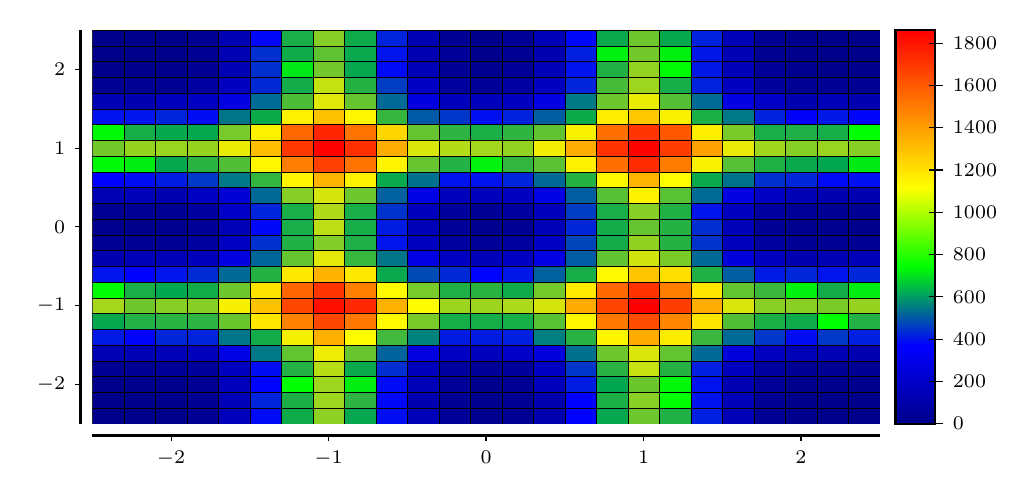
\begin{tikzpicture}[]
\begin{scope}[]
\pgfpathmoveto{ \pgfpointadd{\pgfpointxy {0.0} {0.0}} {\pgfpoint{0cm}{0cm}} }
\pgfpathlineto{ \pgfpointadd{\pgfpointxy {0.0} {0.0}} {\pgfpoint{10cm}{0cm}} }
\pgfpathlineto{ \pgfpointadd{\pgfpointxy {0.0} {0.0}} {\pgfpoint{10cm}{5cm}} }
\pgfpathlineto{ \pgfpointadd{\pgfpointxy {0.0} {0.0}} {\pgfpoint{0cm}{5cm}} }
\pgfpathclose
\pgfusepath{  clip, }
\begin{scope}[shift={(0.0,0.0)}]
\pgfsetxvec{\pgfpoint{2.0cm}{0cm}}
\pgfsetyvec{\pgfpoint{0cm}{1.0cm}}
\begin{scope}[shift={(2.5,2.5)}]
\begin{scope}[draw=black,ultra thin, fill=blue!0!DarkBlue]
\pgfpathmoveto{ \pgfpointxy {-2.5} {-2.5}}
\pgfpathlineto{ \pgfpointxy {-2.3} {-2.5}}
\pgfpathlineto{ \pgfpointxy {-2.3} {-2.3}}
\pgfpathlineto{ \pgfpointxy {-2.5} {-2.3}}
\pgfpathclose
\pgfusepath{ stroke, fill, }
\end{scope}
\begin{scope}[draw=black,ultra thin, fill=blue!0!DarkBlue]
\pgfpathmoveto{ \pgfpointxy {-2.3} {-2.5}}
\pgfpathlineto{ \pgfpointxy {-2.0999999999999996} {-2.5}}
\pgfpathlineto{ \pgfpointxy {-2.0999999999999996} {-2.3}}
\pgfpathlineto{ \pgfpointxy {-2.3} {-2.3}}
\pgfpathclose
\pgfusepath{ stroke, fill, }
\end{scope}
\begin{scope}[draw=black,ultra thin, fill=blue!0!DarkBlue]
\pgfpathmoveto{ \pgfpointxy {-2.1} {-2.5}}
\pgfpathlineto{ \pgfpointxy {-1.9000000000000001} {-2.5}}
\pgfpathlineto{ \pgfpointxy {-1.9000000000000001} {-2.3}}
\pgfpathlineto{ \pgfpointxy {-2.1} {-2.3}}
\pgfpathclose
\pgfusepath{ stroke, fill, }
\end{scope}
\begin{scope}[draw=black,ultra thin, fill=blue!8!DarkBlue]
\pgfpathmoveto{ \pgfpointxy {-1.9} {-2.5}}
\pgfpathlineto{ \pgfpointxy {-1.7} {-2.5}}
\pgfpathlineto{ \pgfpointxy {-1.7} {-2.3}}
\pgfpathlineto{ \pgfpointxy {-1.9} {-2.3}}
\pgfpathclose
\pgfusepath{ stroke, fill, }
\end{scope}
\begin{scope}[draw=black,ultra thin, fill=blue!42!DarkBlue]
\pgfpathmoveto{ \pgfpointxy {-1.7} {-2.5}}
\pgfpathlineto{ \pgfpointxy {-1.5} {-2.5}}
\pgfpathlineto{ \pgfpointxy {-1.5} {-2.3}}
\pgfpathlineto{ \pgfpointxy {-1.7} {-2.3}}
\pgfpathclose
\pgfusepath{ stroke, fill, }
\end{scope}
\begin{scope}[draw=black,ultra thin, fill=green!4!blue]
\pgfpathmoveto{ \pgfpointxy {-1.5} {-2.5}}
\pgfpathlineto{ \pgfpointxy {-1.3} {-2.5}}
\pgfpathlineto{ \pgfpointxy {-1.3} {-2.3}}
\pgfpathlineto{ \pgfpointxy {-1.5} {-2.3}}
\pgfpathclose
\pgfusepath{ stroke, fill, }
\end{scope}
\begin{scope}[draw=black,ultra thin, fill=yellow!6!green]
\pgfpathmoveto{ \pgfpointxy {-1.2999999999999998} {-2.5}}
\pgfpathlineto{ \pgfpointxy {-1.0999999999999999} {-2.5}}
\pgfpathlineto{ \pgfpointxy {-1.0999999999999999} {-2.3}}
\pgfpathlineto{ \pgfpointxy {-1.2999999999999998} {-2.3}}
\pgfpathclose
\pgfusepath{ stroke, fill, }
\end{scope}
\begin{scope}[draw=black,ultra thin, fill=yellow!56!green]
\pgfpathmoveto{ \pgfpointxy {-1.0999999999999999} {-2.5}}
\pgfpathlineto{ \pgfpointxy {-0.8999999999999999} {-2.5}}
\pgfpathlineto{ \pgfpointxy {-0.8999999999999999} {-2.3}}
\pgfpathlineto{ \pgfpointxy {-1.0999999999999999} {-2.3}}
\pgfpathclose
\pgfusepath{ stroke, fill, }
\end{scope}
\begin{scope}[draw=black,ultra thin, fill=yellow!2!green]
\pgfpathmoveto{ \pgfpointxy {-0.8999999999999999} {-2.5}}
\pgfpathlineto{ \pgfpointxy {-0.7} {-2.5}}
\pgfpathlineto{ \pgfpointxy {-0.7} {-2.3}}
\pgfpathlineto{ \pgfpointxy {-0.8999999999999999} {-2.3}}
\pgfpathclose
\pgfusepath{ stroke, fill, }
\end{scope}
\begin{scope}[draw=black,ultra thin, fill=green!5!blue]
\pgfpathmoveto{ \pgfpointxy {-0.7} {-2.5}}
\pgfpathlineto{ \pgfpointxy {-0.49999999999999994} {-2.5}}
\pgfpathlineto{ \pgfpointxy {-0.49999999999999994} {-2.3}}
\pgfpathlineto{ \pgfpointxy {-0.7} {-2.3}}
\pgfpathclose
\pgfusepath{ stroke, fill, }
\end{scope}
\begin{scope}[draw=black,ultra thin, fill=blue!39!DarkBlue]
\pgfpathmoveto{ \pgfpointxy {-0.5} {-2.5}}
\pgfpathlineto{ \pgfpointxy {-0.3} {-2.5}}
\pgfpathlineto{ \pgfpointxy {-0.3} {-2.3}}
\pgfpathlineto{ \pgfpointxy {-0.5} {-2.3}}
\pgfpathclose
\pgfusepath{ stroke, fill, }
\end{scope}
\begin{scope}[draw=black,ultra thin, fill=blue!10!DarkBlue]
\pgfpathmoveto{ \pgfpointxy {-0.2999999999999998} {-2.5}}
\pgfpathlineto{ \pgfpointxy {-0.09999999999999981} {-2.5}}
\pgfpathlineto{ \pgfpointxy {-0.09999999999999981} {-2.3}}
\pgfpathlineto{ \pgfpointxy {-0.2999999999999998} {-2.3}}
\pgfpathclose
\pgfusepath{ stroke, fill, }
\end{scope}
\begin{scope}[draw=black,ultra thin, fill=blue!3!DarkBlue]
\pgfpathmoveto{ \pgfpointxy {-0.09999999999999964} {-2.5}}
\pgfpathlineto{ \pgfpointxy {0.10000000000000037} {-2.5}}
\pgfpathlineto{ \pgfpointxy {0.10000000000000037} {-2.3}}
\pgfpathlineto{ \pgfpointxy {-0.09999999999999964} {-2.3}}
\pgfpathclose
\pgfusepath{ stroke, fill, }
\end{scope}
\begin{scope}[draw=black,ultra thin, fill=blue!7!DarkBlue]
\pgfpathmoveto{ \pgfpointxy {0.10000000000000009} {-2.5}}
\pgfpathlineto{ \pgfpointxy {0.3000000000000001} {-2.5}}
\pgfpathlineto{ \pgfpointxy {0.3000000000000001} {-2.3}}
\pgfpathlineto{ \pgfpointxy {0.10000000000000009} {-2.3}}
\pgfpathclose
\pgfusepath{ stroke, fill, }
\end{scope}
\begin{scope}[draw=black,ultra thin, fill=blue!31!DarkBlue]
\pgfpathmoveto{ \pgfpointxy {0.30000000000000027} {-2.5}}
\pgfpathlineto{ \pgfpointxy {0.5000000000000002} {-2.5}}
\pgfpathlineto{ \pgfpointxy {0.5000000000000002} {-2.3}}
\pgfpathlineto{ \pgfpointxy {0.30000000000000027} {-2.3}}
\pgfpathclose
\pgfusepath{ stroke, fill, }
\end{scope}
\begin{scope}[draw=black,ultra thin, fill=blue!99!DarkBlue]
\pgfpathmoveto{ \pgfpointxy {0.5} {-2.5}}
\pgfpathlineto{ \pgfpointxy {0.7} {-2.5}}
\pgfpathlineto{ \pgfpointxy {0.7} {-2.3}}
\pgfpathlineto{ \pgfpointxy {0.5} {-2.3}}
\pgfpathclose
\pgfusepath{ stroke, fill, }
\end{scope}
\begin{scope}[draw=black,ultra thin, fill=yellow!2!green]
\pgfpathmoveto{ \pgfpointxy {0.7000000000000002} {-2.5}}
\pgfpathlineto{ \pgfpointxy {0.9000000000000001} {-2.5}}
\pgfpathlineto{ \pgfpointxy {0.9000000000000001} {-2.3}}
\pgfpathlineto{ \pgfpointxy {0.7000000000000002} {-2.3}}
\pgfpathclose
\pgfusepath{ stroke, fill, }
\end{scope}
\begin{scope}[draw=black,ultra thin, fill=yellow!43!green]
\pgfpathmoveto{ \pgfpointxy {0.9000000000000004} {-2.5}}
\pgfpathlineto{ \pgfpointxy {1.1000000000000003} {-2.5}}
\pgfpathlineto{ \pgfpointxy {1.1000000000000003} {-2.3}}
\pgfpathlineto{ \pgfpointxy {0.9000000000000004} {-2.3}}
\pgfpathclose
\pgfusepath{ stroke, fill, }
\end{scope}
\begin{scope}[draw=black,ultra thin, fill=yellow!13!green]
\pgfpathmoveto{ \pgfpointxy {1.1} {-2.5}}
\pgfpathlineto{ \pgfpointxy {1.3} {-2.5}}
\pgfpathlineto{ \pgfpointxy {1.3} {-2.3}}
\pgfpathlineto{ \pgfpointxy {1.1} {-2.3}}
\pgfpathclose
\pgfusepath{ stroke, fill, }
\end{scope}
\begin{scope}[draw=black,ultra thin, fill=green!12!blue]
\pgfpathmoveto{ \pgfpointxy {1.3000000000000003} {-2.5}}
\pgfpathlineto{ \pgfpointxy {1.5000000000000002} {-2.5}}
\pgfpathlineto{ \pgfpointxy {1.5000000000000002} {-2.3}}
\pgfpathlineto{ \pgfpointxy {1.3000000000000003} {-2.3}}
\pgfpathclose
\pgfusepath{ stroke, fill, }
\end{scope}
\begin{scope}[draw=black,ultra thin, fill=blue!37!DarkBlue]
\pgfpathmoveto{ \pgfpointxy {1.5} {-2.5}}
\pgfpathlineto{ \pgfpointxy {1.7} {-2.5}}
\pgfpathlineto{ \pgfpointxy {1.7} {-2.3}}
\pgfpathlineto{ \pgfpointxy {1.5} {-2.3}}
\pgfpathclose
\pgfusepath{ stroke, fill, }
\end{scope}
\begin{scope}[draw=black,ultra thin, fill=blue!7!DarkBlue]
\pgfpathmoveto{ \pgfpointxy {1.7000000000000002} {-2.5}}
\pgfpathlineto{ \pgfpointxy {1.9000000000000001} {-2.5}}
\pgfpathlineto{ \pgfpointxy {1.9000000000000001} {-2.3}}
\pgfpathlineto{ \pgfpointxy {1.7000000000000002} {-2.3}}
\pgfpathclose
\pgfusepath{ stroke, fill, }
\end{scope}
\begin{scope}[draw=black,ultra thin, fill=blue!1!DarkBlue]
\pgfpathmoveto{ \pgfpointxy {1.9000000000000004} {-2.5}}
\pgfpathlineto{ \pgfpointxy {2.1000000000000005} {-2.5}}
\pgfpathlineto{ \pgfpointxy {2.1000000000000005} {-2.3}}
\pgfpathlineto{ \pgfpointxy {1.9000000000000004} {-2.3}}
\pgfpathclose
\pgfusepath{ stroke, fill, }
\end{scope}
\begin{scope}[draw=black,ultra thin, fill=blue!0!DarkBlue]
\pgfpathmoveto{ \pgfpointxy {2.1000000000000005} {-2.5}}
\pgfpathlineto{ \pgfpointxy {2.3000000000000007} {-2.5}}
\pgfpathlineto{ \pgfpointxy {2.3000000000000007} {-2.3}}
\pgfpathlineto{ \pgfpointxy {2.1000000000000005} {-2.3}}
\pgfpathclose
\pgfusepath{ stroke, fill, }
\end{scope}
\begin{scope}[draw=black,ultra thin, fill=blue!0!DarkBlue]
\pgfpathmoveto{ \pgfpointxy {2.3000000000000007} {-2.5}}
\pgfpathlineto{ \pgfpointxy {2.500000000000001} {-2.5}}
\pgfpathlineto{ \pgfpointxy {2.500000000000001} {-2.3}}
\pgfpathlineto{ \pgfpointxy {2.3000000000000007} {-2.3}}
\pgfpathclose
\pgfusepath{ stroke, fill, }
\end{scope}
\begin{scope}[draw=black,ultra thin, fill=blue!0!DarkBlue]
\pgfpathmoveto{ \pgfpointxy {-2.5} {-2.3}}
\pgfpathlineto{ \pgfpointxy {-2.3} {-2.3}}
\pgfpathlineto{ \pgfpointxy {-2.3} {-2.0999999999999996}}
\pgfpathlineto{ \pgfpointxy {-2.5} {-2.0999999999999996}}
\pgfpathclose
\pgfusepath{ stroke, fill, }
\end{scope}
\begin{scope}[draw=black,ultra thin, fill=blue!0!DarkBlue]
\pgfpathmoveto{ \pgfpointxy {-2.3} {-2.3}}
\pgfpathlineto{ \pgfpointxy {-2.0999999999999996} {-2.3}}
\pgfpathlineto{ \pgfpointxy {-2.0999999999999996} {-2.0999999999999996}}
\pgfpathlineto{ \pgfpointxy {-2.3} {-2.0999999999999996}}
\pgfpathclose
\pgfusepath{ stroke, fill, }
\end{scope}
\begin{scope}[draw=black,ultra thin, fill=blue!1!DarkBlue]
\pgfpathmoveto{ \pgfpointxy {-2.1} {-2.3}}
\pgfpathlineto{ \pgfpointxy {-1.9000000000000001} {-2.3}}
\pgfpathlineto{ \pgfpointxy {-1.9000000000000001} {-2.0999999999999996}}
\pgfpathlineto{ \pgfpointxy {-2.1} {-2.0999999999999996}}
\pgfpathclose
\pgfusepath{ stroke, fill, }
\end{scope}
\begin{scope}[draw=black,ultra thin, fill=blue!6!DarkBlue]
\pgfpathmoveto{ \pgfpointxy {-1.9} {-2.3}}
\pgfpathlineto{ \pgfpointxy {-1.7} {-2.3}}
\pgfpathlineto{ \pgfpointxy {-1.7} {-2.0999999999999996}}
\pgfpathlineto{ \pgfpointxy {-1.9} {-2.0999999999999996}}
\pgfpathclose
\pgfusepath{ stroke, fill, }
\end{scope}
\begin{scope}[draw=black,ultra thin, fill=blue!40!DarkBlue]
\pgfpathmoveto{ \pgfpointxy {-1.7} {-2.3}}
\pgfpathlineto{ \pgfpointxy {-1.5} {-2.3}}
\pgfpathlineto{ \pgfpointxy {-1.5} {-2.0999999999999996}}
\pgfpathlineto{ \pgfpointxy {-1.7} {-2.0999999999999996}}
\pgfpathclose
\pgfusepath{ stroke, fill, }
\end{scope}
\begin{scope}[draw=black,ultra thin, fill=green!14!blue]
\pgfpathmoveto{ \pgfpointxy {-1.5} {-2.3}}
\pgfpathlineto{ \pgfpointxy {-1.3} {-2.3}}
\pgfpathlineto{ \pgfpointxy {-1.3} {-2.0999999999999996}}
\pgfpathlineto{ \pgfpointxy {-1.5} {-2.0999999999999996}}
\pgfpathclose
\pgfusepath{ stroke, fill, }
\end{scope}
\begin{scope}[draw=black,ultra thin, fill=yellow!11!green]
\pgfpathmoveto{ \pgfpointxy {-1.2999999999999998} {-2.3}}
\pgfpathlineto{ \pgfpointxy {-1.0999999999999999} {-2.3}}
\pgfpathlineto{ \pgfpointxy {-1.0999999999999999} {-2.0999999999999996}}
\pgfpathlineto{ \pgfpointxy {-1.2999999999999998} {-2.0999999999999996}}
\pgfpathclose
\pgfusepath{ stroke, fill, }
\end{scope}
\begin{scope}[draw=black,ultra thin, fill=yellow!62!green]
\pgfpathmoveto{ \pgfpointxy {-1.0999999999999999} {-2.3}}
\pgfpathlineto{ \pgfpointxy {-0.8999999999999999} {-2.3}}
\pgfpathlineto{ \pgfpointxy {-0.8999999999999999} {-2.0999999999999996}}
\pgfpathlineto{ \pgfpointxy {-1.0999999999999999} {-2.0999999999999996}}
\pgfpathclose
\pgfusepath{ stroke, fill, }
\end{scope}
\begin{scope}[draw=black,ultra thin, fill=yellow!18!green]
\pgfpathmoveto{ \pgfpointxy {-0.8999999999999999} {-2.3}}
\pgfpathlineto{ \pgfpointxy {-0.7} {-2.3}}
\pgfpathlineto{ \pgfpointxy {-0.7} {-2.0999999999999996}}
\pgfpathlineto{ \pgfpointxy {-0.8999999999999999} {-2.0999999999999996}}
\pgfpathclose
\pgfusepath{ stroke, fill, }
\end{scope}
\begin{scope}[draw=black,ultra thin, fill=green!3!blue]
\pgfpathmoveto{ \pgfpointxy {-0.7} {-2.3}}
\pgfpathlineto{ \pgfpointxy {-0.49999999999999994} {-2.3}}
\pgfpathlineto{ \pgfpointxy {-0.49999999999999994} {-2.0999999999999996}}
\pgfpathlineto{ \pgfpointxy {-0.7} {-2.0999999999999996}}
\pgfpathclose
\pgfusepath{ stroke, fill, }
\end{scope}
\begin{scope}[draw=black,ultra thin, fill=blue!33!DarkBlue]
\pgfpathmoveto{ \pgfpointxy {-0.5} {-2.3}}
\pgfpathlineto{ \pgfpointxy {-0.3} {-2.3}}
\pgfpathlineto{ \pgfpointxy {-0.3} {-2.0999999999999996}}
\pgfpathlineto{ \pgfpointxy {-0.5} {-2.0999999999999996}}
\pgfpathclose
\pgfusepath{ stroke, fill, }
\end{scope}
\begin{scope}[draw=black,ultra thin, fill=blue!8!DarkBlue]
\pgfpathmoveto{ \pgfpointxy {-0.2999999999999998} {-2.3}}
\pgfpathlineto{ \pgfpointxy {-0.09999999999999981} {-2.3}}
\pgfpathlineto{ \pgfpointxy {-0.09999999999999981} {-2.0999999999999996}}
\pgfpathlineto{ \pgfpointxy {-0.2999999999999998} {-2.0999999999999996}}
\pgfpathclose
\pgfusepath{ stroke, fill, }
\end{scope}
\begin{scope}[draw=black,ultra thin, fill=blue!3!DarkBlue]
\pgfpathmoveto{ \pgfpointxy {-0.09999999999999964} {-2.3}}
\pgfpathlineto{ \pgfpointxy {0.10000000000000037} {-2.3}}
\pgfpathlineto{ \pgfpointxy {0.10000000000000037} {-2.0999999999999996}}
\pgfpathlineto{ \pgfpointxy {-0.09999999999999964} {-2.0999999999999996}}
\pgfpathclose
\pgfusepath{ stroke, fill, }
\end{scope}
\begin{scope}[draw=black,ultra thin, fill=blue!7!DarkBlue]
\pgfpathmoveto{ \pgfpointxy {0.10000000000000009} {-2.3}}
\pgfpathlineto{ \pgfpointxy {0.3000000000000001} {-2.3}}
\pgfpathlineto{ \pgfpointxy {0.3000000000000001} {-2.0999999999999996}}
\pgfpathlineto{ \pgfpointxy {0.10000000000000009} {-2.0999999999999996}}
\pgfpathclose
\pgfusepath{ stroke, fill, }
\end{scope}
\begin{scope}[draw=black,ultra thin, fill=blue!31!DarkBlue]
\pgfpathmoveto{ \pgfpointxy {0.30000000000000027} {-2.3}}
\pgfpathlineto{ \pgfpointxy {0.5000000000000002} {-2.3}}
\pgfpathlineto{ \pgfpointxy {0.5000000000000002} {-2.0999999999999996}}
\pgfpathlineto{ \pgfpointxy {0.30000000000000027} {-2.0999999999999996}}
\pgfpathclose
\pgfusepath{ stroke, fill, }
\end{scope}
\begin{scope}[draw=black,ultra thin, fill=green!0!blue]
\pgfpathmoveto{ \pgfpointxy {0.5} {-2.3}}
\pgfpathlineto{ \pgfpointxy {0.7} {-2.3}}
\pgfpathlineto{ \pgfpointxy {0.7} {-2.0999999999999996}}
\pgfpathlineto{ \pgfpointxy {0.5} {-2.0999999999999996}}
\pgfpathclose
\pgfusepath{ stroke, fill, }
\end{scope}
\begin{scope}[draw=black,ultra thin, fill=yellow!11!green]
\pgfpathmoveto{ \pgfpointxy {0.7000000000000002} {-2.3}}
\pgfpathlineto{ \pgfpointxy {0.9000000000000001} {-2.3}}
\pgfpathlineto{ \pgfpointxy {0.9000000000000001} {-2.0999999999999996}}
\pgfpathlineto{ \pgfpointxy {0.7000000000000002} {-2.0999999999999996}}
\pgfpathclose
\pgfusepath{ stroke, fill, }
\end{scope}
\begin{scope}[draw=black,ultra thin, fill=yellow!54!green]
\pgfpathmoveto{ \pgfpointxy {0.9000000000000004} {-2.3}}
\pgfpathlineto{ \pgfpointxy {1.1000000000000003} {-2.3}}
\pgfpathlineto{ \pgfpointxy {1.1000000000000003} {-2.0999999999999996}}
\pgfpathlineto{ \pgfpointxy {0.9000000000000004} {-2.0999999999999996}}
\pgfpathclose
\pgfusepath{ stroke, fill, }
\end{scope}
\begin{scope}[draw=black,ultra thin, fill=yellow!0!green]
\pgfpathmoveto{ \pgfpointxy {1.1} {-2.3}}
\pgfpathlineto{ \pgfpointxy {1.3} {-2.3}}
\pgfpathlineto{ \pgfpointxy {1.3} {-2.0999999999999996}}
\pgfpathlineto{ \pgfpointxy {1.1} {-2.0999999999999996}}
\pgfpathclose
\pgfusepath{ stroke, fill, }
\end{scope}
\begin{scope}[draw=black,ultra thin, fill=green!7!blue]
\pgfpathmoveto{ \pgfpointxy {1.3000000000000003} {-2.3}}
\pgfpathlineto{ \pgfpointxy {1.5000000000000002} {-2.3}}
\pgfpathlineto{ \pgfpointxy {1.5000000000000002} {-2.0999999999999996}}
\pgfpathlineto{ \pgfpointxy {1.3000000000000003} {-2.0999999999999996}}
\pgfpathclose
\pgfusepath{ stroke, fill, }
\end{scope}
\begin{scope}[draw=black,ultra thin, fill=blue!39!DarkBlue]
\pgfpathmoveto{ \pgfpointxy {1.5} {-2.3}}
\pgfpathlineto{ \pgfpointxy {1.7} {-2.3}}
\pgfpathlineto{ \pgfpointxy {1.7} {-2.0999999999999996}}
\pgfpathlineto{ \pgfpointxy {1.5} {-2.0999999999999996}}
\pgfpathclose
\pgfusepath{ stroke, fill, }
\end{scope}
\begin{scope}[draw=black,ultra thin, fill=blue!8!DarkBlue]
\pgfpathmoveto{ \pgfpointxy {1.7000000000000002} {-2.3}}
\pgfpathlineto{ \pgfpointxy {1.9000000000000001} {-2.3}}
\pgfpathlineto{ \pgfpointxy {1.9000000000000001} {-2.0999999999999996}}
\pgfpathlineto{ \pgfpointxy {1.7000000000000002} {-2.0999999999999996}}
\pgfpathclose
\pgfusepath{ stroke, fill, }
\end{scope}
\begin{scope}[draw=black,ultra thin, fill=blue!0!DarkBlue]
\pgfpathmoveto{ \pgfpointxy {1.9000000000000004} {-2.3}}
\pgfpathlineto{ \pgfpointxy {2.1000000000000005} {-2.3}}
\pgfpathlineto{ \pgfpointxy {2.1000000000000005} {-2.0999999999999996}}
\pgfpathlineto{ \pgfpointxy {1.9000000000000004} {-2.0999999999999996}}
\pgfpathclose
\pgfusepath{ stroke, fill, }
\end{scope}
\begin{scope}[draw=black,ultra thin, fill=blue!0!DarkBlue]
\pgfpathmoveto{ \pgfpointxy {2.1000000000000005} {-2.3}}
\pgfpathlineto{ \pgfpointxy {2.3000000000000007} {-2.3}}
\pgfpathlineto{ \pgfpointxy {2.3000000000000007} {-2.0999999999999996}}
\pgfpathlineto{ \pgfpointxy {2.1000000000000005} {-2.0999999999999996}}
\pgfpathclose
\pgfusepath{ stroke, fill, }
\end{scope}
\begin{scope}[draw=black,ultra thin, fill=blue!0!DarkBlue]
\pgfpathmoveto{ \pgfpointxy {2.3000000000000007} {-2.3}}
\pgfpathlineto{ \pgfpointxy {2.500000000000001} {-2.3}}
\pgfpathlineto{ \pgfpointxy {2.500000000000001} {-2.0999999999999996}}
\pgfpathlineto{ \pgfpointxy {2.3000000000000007} {-2.0999999999999996}}
\pgfpathclose
\pgfusepath{ stroke, fill, }
\end{scope}
\begin{scope}[draw=black,ultra thin, fill=blue!0!DarkBlue]
\pgfpathmoveto{ \pgfpointxy {-2.5} {-2.1}}
\pgfpathlineto{ \pgfpointxy {-2.3} {-2.1}}
\pgfpathlineto{ \pgfpointxy {-2.3} {-1.9000000000000001}}
\pgfpathlineto{ \pgfpointxy {-2.5} {-1.9000000000000001}}
\pgfpathclose
\pgfusepath{ stroke, fill, }
\end{scope}
\begin{scope}[draw=black,ultra thin, fill=blue!1!DarkBlue]
\pgfpathmoveto{ \pgfpointxy {-2.3} {-2.1}}
\pgfpathlineto{ \pgfpointxy {-2.0999999999999996} {-2.1}}
\pgfpathlineto{ \pgfpointxy {-2.0999999999999996} {-1.9000000000000001}}
\pgfpathlineto{ \pgfpointxy {-2.3} {-1.9000000000000001}}
\pgfpathclose
\pgfusepath{ stroke, fill, }
\end{scope}
\begin{scope}[draw=black,ultra thin, fill=blue!2!DarkBlue]
\pgfpathmoveto{ \pgfpointxy {-2.1} {-2.1}}
\pgfpathlineto{ \pgfpointxy {-1.9000000000000001} {-2.1}}
\pgfpathlineto{ \pgfpointxy {-1.9000000000000001} {-1.9000000000000001}}
\pgfpathlineto{ \pgfpointxy {-2.1} {-1.9000000000000001}}
\pgfpathclose
\pgfusepath{ stroke, fill, }
\end{scope}
\begin{scope}[draw=black,ultra thin, fill=blue!7!DarkBlue]
\pgfpathmoveto{ \pgfpointxy {-1.9} {-2.1}}
\pgfpathlineto{ \pgfpointxy {-1.7} {-2.1}}
\pgfpathlineto{ \pgfpointxy {-1.7} {-1.9000000000000001}}
\pgfpathlineto{ \pgfpointxy {-1.9} {-1.9000000000000001}}
\pgfpathclose
\pgfusepath{ stroke, fill, }
\end{scope}
\begin{scope}[draw=black,ultra thin, fill=blue!42!DarkBlue]
\pgfpathmoveto{ \pgfpointxy {-1.7} {-2.1}}
\pgfpathlineto{ \pgfpointxy {-1.5} {-2.1}}
\pgfpathlineto{ \pgfpointxy {-1.5} {-1.9000000000000001}}
\pgfpathlineto{ \pgfpointxy {-1.7} {-1.9000000000000001}}
\pgfpathclose
\pgfusepath{ stroke, fill, }
\end{scope}
\begin{scope}[draw=black,ultra thin, fill=green!1!blue]
\pgfpathmoveto{ \pgfpointxy {-1.5} {-2.1}}
\pgfpathlineto{ \pgfpointxy {-1.3} {-2.1}}
\pgfpathlineto{ \pgfpointxy {-1.3} {-1.9000000000000001}}
\pgfpathlineto{ \pgfpointxy {-1.5} {-1.9000000000000001}}
\pgfpathclose
\pgfusepath{ stroke, fill, }
\end{scope}
\begin{scope}[draw=black,ultra thin, fill=yellow!0!green]
\pgfpathmoveto{ \pgfpointxy {-1.2999999999999998} {-2.1}}
\pgfpathlineto{ \pgfpointxy {-1.0999999999999999} {-2.1}}
\pgfpathlineto{ \pgfpointxy {-1.0999999999999999} {-1.9000000000000001}}
\pgfpathlineto{ \pgfpointxy {-1.2999999999999998} {-1.9000000000000001}}
\pgfpathclose
\pgfusepath{ stroke, fill, }
\end{scope}
\begin{scope}[draw=black,ultra thin, fill=yellow!62!green]
\pgfpathmoveto{ \pgfpointxy {-1.0999999999999999} {-2.1}}
\pgfpathlineto{ \pgfpointxy {-0.8999999999999999} {-2.1}}
\pgfpathlineto{ \pgfpointxy {-0.8999999999999999} {-1.9000000000000001}}
\pgfpathlineto{ \pgfpointxy {-1.0999999999999999} {-1.9000000000000001}}
\pgfpathclose
\pgfusepath{ stroke, fill, }
\end{scope}
\begin{scope}[draw=black,ultra thin, fill=green!93!blue]
\pgfpathmoveto{ \pgfpointxy {-0.8999999999999999} {-2.1}}
\pgfpathlineto{ \pgfpointxy {-0.7} {-2.1}}
\pgfpathlineto{ \pgfpointxy {-0.7} {-1.9000000000000001}}
\pgfpathlineto{ \pgfpointxy {-0.8999999999999999} {-1.9000000000000001}}
\pgfpathclose
\pgfusepath{ stroke, fill, }
\end{scope}
\begin{scope}[draw=black,ultra thin, fill=green!4!blue]
\pgfpathmoveto{ \pgfpointxy {-0.7} {-2.1}}
\pgfpathlineto{ \pgfpointxy {-0.49999999999999994} {-2.1}}
\pgfpathlineto{ \pgfpointxy {-0.49999999999999994} {-1.9000000000000001}}
\pgfpathlineto{ \pgfpointxy {-0.7} {-1.9000000000000001}}
\pgfpathclose
\pgfusepath{ stroke, fill, }
\end{scope}
\begin{scope}[draw=black,ultra thin, fill=blue!38!DarkBlue]
\pgfpathmoveto{ \pgfpointxy {-0.5} {-2.1}}
\pgfpathlineto{ \pgfpointxy {-0.3} {-2.1}}
\pgfpathlineto{ \pgfpointxy {-0.3} {-1.9000000000000001}}
\pgfpathlineto{ \pgfpointxy {-0.5} {-1.9000000000000001}}
\pgfpathclose
\pgfusepath{ stroke, fill, }
\end{scope}
\begin{scope}[draw=black,ultra thin, fill=blue!10!DarkBlue]
\pgfpathmoveto{ \pgfpointxy {-0.2999999999999998} {-2.1}}
\pgfpathlineto{ \pgfpointxy {-0.09999999999999981} {-2.1}}
\pgfpathlineto{ \pgfpointxy {-0.09999999999999981} {-1.9000000000000001}}
\pgfpathlineto{ \pgfpointxy {-0.2999999999999998} {-1.9000000000000001}}
\pgfpathclose
\pgfusepath{ stroke, fill, }
\end{scope}
\begin{scope}[draw=black,ultra thin, fill=blue!2!DarkBlue]
\pgfpathmoveto{ \pgfpointxy {-0.09999999999999964} {-2.1}}
\pgfpathlineto{ \pgfpointxy {0.10000000000000037} {-2.1}}
\pgfpathlineto{ \pgfpointxy {0.10000000000000037} {-1.9000000000000001}}
\pgfpathlineto{ \pgfpointxy {-0.09999999999999964} {-1.9000000000000001}}
\pgfpathclose
\pgfusepath{ stroke, fill, }
\end{scope}
\begin{scope}[draw=black,ultra thin, fill=blue!9!DarkBlue]
\pgfpathmoveto{ \pgfpointxy {0.10000000000000009} {-2.1}}
\pgfpathlineto{ \pgfpointxy {0.3000000000000001} {-2.1}}
\pgfpathlineto{ \pgfpointxy {0.3000000000000001} {-1.9000000000000001}}
\pgfpathlineto{ \pgfpointxy {0.10000000000000009} {-1.9000000000000001}}
\pgfpathclose
\pgfusepath{ stroke, fill, }
\end{scope}
\begin{scope}[draw=black,ultra thin, fill=blue!41!DarkBlue]
\pgfpathmoveto{ \pgfpointxy {0.30000000000000027} {-2.1}}
\pgfpathlineto{ \pgfpointxy {0.5000000000000002} {-2.1}}
\pgfpathlineto{ \pgfpointxy {0.5000000000000002} {-1.9000000000000001}}
\pgfpathlineto{ \pgfpointxy {0.30000000000000027} {-1.9000000000000001}}
\pgfpathclose
\pgfusepath{ stroke, fill, }
\end{scope}
\begin{scope}[draw=black,ultra thin, fill=green!11!blue]
\pgfpathmoveto{ \pgfpointxy {0.5} {-2.1}}
\pgfpathlineto{ \pgfpointxy {0.7} {-2.1}}
\pgfpathlineto{ \pgfpointxy {0.7} {-1.9000000000000001}}
\pgfpathlineto{ \pgfpointxy {0.5} {-1.9000000000000001}}
\pgfpathclose
\pgfusepath{ stroke, fill, }
\end{scope}
\begin{scope}[draw=black,ultra thin, fill=yellow!1!green]
\pgfpathmoveto{ \pgfpointxy {0.7000000000000002} {-2.1}}
\pgfpathlineto{ \pgfpointxy {0.9000000000000001} {-2.1}}
\pgfpathlineto{ \pgfpointxy {0.9000000000000001} {-1.9000000000000001}}
\pgfpathlineto{ \pgfpointxy {0.7000000000000002} {-1.9000000000000001}}
\pgfpathclose
\pgfusepath{ stroke, fill, }
\end{scope}
\begin{scope}[draw=black,ultra thin, fill=yellow!42!green]
\pgfpathmoveto{ \pgfpointxy {0.9000000000000004} {-2.1}}
\pgfpathlineto{ \pgfpointxy {1.1000000000000003} {-2.1}}
\pgfpathlineto{ \pgfpointxy {1.1000000000000003} {-1.9000000000000001}}
\pgfpathlineto{ \pgfpointxy {0.9000000000000004} {-1.9000000000000001}}
\pgfpathclose
\pgfusepath{ stroke, fill, }
\end{scope}
\begin{scope}[draw=black,ultra thin, fill=green!97!blue]
\pgfpathmoveto{ \pgfpointxy {1.1} {-2.1}}
\pgfpathlineto{ \pgfpointxy {1.3} {-2.1}}
\pgfpathlineto{ \pgfpointxy {1.3} {-1.9000000000000001}}
\pgfpathlineto{ \pgfpointxy {1.1} {-1.9000000000000001}}
\pgfpathclose
\pgfusepath{ stroke, fill, }
\end{scope}
\begin{scope}[draw=black,ultra thin, fill=green!7!blue]
\pgfpathmoveto{ \pgfpointxy {1.3000000000000003} {-2.1}}
\pgfpathlineto{ \pgfpointxy {1.5000000000000002} {-2.1}}
\pgfpathlineto{ \pgfpointxy {1.5000000000000002} {-1.9000000000000001}}
\pgfpathlineto{ \pgfpointxy {1.3000000000000003} {-1.9000000000000001}}
\pgfpathclose
\pgfusepath{ stroke, fill, }
\end{scope}
\begin{scope}[draw=black,ultra thin, fill=blue!34!DarkBlue]
\pgfpathmoveto{ \pgfpointxy {1.5} {-2.1}}
\pgfpathlineto{ \pgfpointxy {1.7} {-2.1}}
\pgfpathlineto{ \pgfpointxy {1.7} {-1.9000000000000001}}
\pgfpathlineto{ \pgfpointxy {1.5} {-1.9000000000000001}}
\pgfpathclose
\pgfusepath{ stroke, fill, }
\end{scope}
\begin{scope}[draw=black,ultra thin, fill=blue!11!DarkBlue]
\pgfpathmoveto{ \pgfpointxy {1.7000000000000002} {-2.1}}
\pgfpathlineto{ \pgfpointxy {1.9000000000000001} {-2.1}}
\pgfpathlineto{ \pgfpointxy {1.9000000000000001} {-1.9000000000000001}}
\pgfpathlineto{ \pgfpointxy {1.7000000000000002} {-1.9000000000000001}}
\pgfpathclose
\pgfusepath{ stroke, fill, }
\end{scope}
\begin{scope}[draw=black,ultra thin, fill=blue!1!DarkBlue]
\pgfpathmoveto{ \pgfpointxy {1.9000000000000004} {-2.1}}
\pgfpathlineto{ \pgfpointxy {2.1000000000000005} {-2.1}}
\pgfpathlineto{ \pgfpointxy {2.1000000000000005} {-1.9000000000000001}}
\pgfpathlineto{ \pgfpointxy {1.9000000000000004} {-1.9000000000000001}}
\pgfpathclose
\pgfusepath{ stroke, fill, }
\end{scope}
\begin{scope}[draw=black,ultra thin, fill=blue!1!DarkBlue]
\pgfpathmoveto{ \pgfpointxy {2.1000000000000005} {-2.1}}
\pgfpathlineto{ \pgfpointxy {2.3000000000000007} {-2.1}}
\pgfpathlineto{ \pgfpointxy {2.3000000000000007} {-1.9000000000000001}}
\pgfpathlineto{ \pgfpointxy {2.1000000000000005} {-1.9000000000000001}}
\pgfpathclose
\pgfusepath{ stroke, fill, }
\end{scope}
\begin{scope}[draw=black,ultra thin, fill=blue!1!DarkBlue]
\pgfpathmoveto{ \pgfpointxy {2.3000000000000007} {-2.1}}
\pgfpathlineto{ \pgfpointxy {2.500000000000001} {-2.1}}
\pgfpathlineto{ \pgfpointxy {2.500000000000001} {-1.9000000000000001}}
\pgfpathlineto{ \pgfpointxy {2.3000000000000007} {-1.9000000000000001}}
\pgfpathclose
\pgfusepath{ stroke, fill, }
\end{scope}
\begin{scope}[draw=black,ultra thin, fill=blue!9!DarkBlue]
\pgfpathmoveto{ \pgfpointxy {-2.5} {-1.9}}
\pgfpathlineto{ \pgfpointxy {-2.3} {-1.9}}
\pgfpathlineto{ \pgfpointxy {-2.3} {-1.7}}
\pgfpathlineto{ \pgfpointxy {-2.5} {-1.7}}
\pgfpathclose
\pgfusepath{ stroke, fill, }
\end{scope}
\begin{scope}[draw=black,ultra thin, fill=blue!7!DarkBlue]
\pgfpathmoveto{ \pgfpointxy {-2.3} {-1.9}}
\pgfpathlineto{ \pgfpointxy {-2.0999999999999996} {-1.9}}
\pgfpathlineto{ \pgfpointxy {-2.0999999999999996} {-1.7}}
\pgfpathlineto{ \pgfpointxy {-2.3} {-1.7}}
\pgfpathclose
\pgfusepath{ stroke, fill, }
\end{scope}
\begin{scope}[draw=black,ultra thin, fill=blue!11!DarkBlue]
\pgfpathmoveto{ \pgfpointxy {-2.1} {-1.9}}
\pgfpathlineto{ \pgfpointxy {-1.9000000000000001} {-1.9}}
\pgfpathlineto{ \pgfpointxy {-1.9000000000000001} {-1.7}}
\pgfpathlineto{ \pgfpointxy {-2.1} {-1.7}}
\pgfpathclose
\pgfusepath{ stroke, fill, }
\end{scope}
\begin{scope}[draw=black,ultra thin, fill=blue!15!DarkBlue]
\pgfpathmoveto{ \pgfpointxy {-1.9} {-1.9}}
\pgfpathlineto{ \pgfpointxy {-1.7} {-1.9}}
\pgfpathlineto{ \pgfpointxy {-1.7} {-1.7}}
\pgfpathlineto{ \pgfpointxy {-1.9} {-1.7}}
\pgfpathclose
\pgfusepath{ stroke, fill, }
\end{scope}
\begin{scope}[draw=black,ultra thin, fill=blue!45!DarkBlue]
\pgfpathmoveto{ \pgfpointxy {-1.7} {-1.9}}
\pgfpathlineto{ \pgfpointxy {-1.5} {-1.9}}
\pgfpathlineto{ \pgfpointxy {-1.5} {-1.7}}
\pgfpathlineto{ \pgfpointxy {-1.7} {-1.7}}
\pgfpathclose
\pgfusepath{ stroke, fill, }
\end{scope}
\begin{scope}[draw=black,ultra thin, fill=green!5!blue]
\pgfpathmoveto{ \pgfpointxy {-1.5} {-1.9}}
\pgfpathlineto{ \pgfpointxy {-1.3} {-1.9}}
\pgfpathlineto{ \pgfpointxy {-1.3} {-1.7}}
\pgfpathlineto{ \pgfpointxy {-1.5} {-1.7}}
\pgfpathclose
\pgfusepath{ stroke, fill, }
\end{scope}
\begin{scope}[draw=black,ultra thin, fill=yellow!14!green]
\pgfpathmoveto{ \pgfpointxy {-1.2999999999999998} {-1.9}}
\pgfpathlineto{ \pgfpointxy {-1.0999999999999999} {-1.9}}
\pgfpathlineto{ \pgfpointxy {-1.0999999999999999} {-1.7}}
\pgfpathlineto{ \pgfpointxy {-1.2999999999999998} {-1.7}}
\pgfpathclose
\pgfusepath{ stroke, fill, }
\end{scope}
\begin{scope}[draw=black,ultra thin, fill=yellow!72!green]
\pgfpathmoveto{ \pgfpointxy {-1.0999999999999999} {-1.9}}
\pgfpathlineto{ \pgfpointxy {-0.8999999999999999} {-1.9}}
\pgfpathlineto{ \pgfpointxy {-0.8999999999999999} {-1.7}}
\pgfpathlineto{ \pgfpointxy {-1.0999999999999999} {-1.7}}
\pgfpathclose
\pgfusepath{ stroke, fill, }
\end{scope}
\begin{scope}[draw=black,ultra thin, fill=yellow!4!green]
\pgfpathmoveto{ \pgfpointxy {-0.8999999999999999} {-1.9}}
\pgfpathlineto{ \pgfpointxy {-0.7} {-1.9}}
\pgfpathlineto{ \pgfpointxy {-0.7} {-1.7}}
\pgfpathlineto{ \pgfpointxy {-0.8999999999999999} {-1.7}}
\pgfpathclose
\pgfusepath{ stroke, fill, }
\end{scope}
\begin{scope}[draw=black,ultra thin, fill=green!18!blue]
\pgfpathmoveto{ \pgfpointxy {-0.7} {-1.9}}
\pgfpathlineto{ \pgfpointxy {-0.49999999999999994} {-1.9}}
\pgfpathlineto{ \pgfpointxy {-0.49999999999999994} {-1.7}}
\pgfpathlineto{ \pgfpointxy {-0.7} {-1.7}}
\pgfpathclose
\pgfusepath{ stroke, fill, }
\end{scope}
\begin{scope}[draw=black,ultra thin, fill=blue!42!DarkBlue]
\pgfpathmoveto{ \pgfpointxy {-0.5} {-1.9}}
\pgfpathlineto{ \pgfpointxy {-0.3} {-1.9}}
\pgfpathlineto{ \pgfpointxy {-0.3} {-1.7}}
\pgfpathlineto{ \pgfpointxy {-0.5} {-1.7}}
\pgfpathclose
\pgfusepath{ stroke, fill, }
\end{scope}
\begin{scope}[draw=black,ultra thin, fill=blue!17!DarkBlue]
\pgfpathmoveto{ \pgfpointxy {-0.2999999999999998} {-1.9}}
\pgfpathlineto{ \pgfpointxy {-0.09999999999999981} {-1.9}}
\pgfpathlineto{ \pgfpointxy {-0.09999999999999981} {-1.7}}
\pgfpathlineto{ \pgfpointxy {-0.2999999999999998} {-1.7}}
\pgfpathclose
\pgfusepath{ stroke, fill, }
\end{scope}
\begin{scope}[draw=black,ultra thin, fill=blue!10!DarkBlue]
\pgfpathmoveto{ \pgfpointxy {-0.09999999999999964} {-1.9}}
\pgfpathlineto{ \pgfpointxy {0.10000000000000037} {-1.9}}
\pgfpathlineto{ \pgfpointxy {0.10000000000000037} {-1.7}}
\pgfpathlineto{ \pgfpointxy {-0.09999999999999964} {-1.7}}
\pgfpathclose
\pgfusepath{ stroke, fill, }
\end{scope}
\begin{scope}[draw=black,ultra thin, fill=blue!15!DarkBlue]
\pgfpathmoveto{ \pgfpointxy {0.10000000000000009} {-1.9}}
\pgfpathlineto{ \pgfpointxy {0.3000000000000001} {-1.9}}
\pgfpathlineto{ \pgfpointxy {0.3000000000000001} {-1.7}}
\pgfpathlineto{ \pgfpointxy {0.10000000000000009} {-1.7}}
\pgfpathclose
\pgfusepath{ stroke, fill, }
\end{scope}
\begin{scope}[draw=black,ultra thin, fill=blue!48!DarkBlue]
\pgfpathmoveto{ \pgfpointxy {0.30000000000000027} {-1.9}}
\pgfpathlineto{ \pgfpointxy {0.5000000000000002} {-1.9}}
\pgfpathlineto{ \pgfpointxy {0.5000000000000002} {-1.7}}
\pgfpathlineto{ \pgfpointxy {0.30000000000000027} {-1.7}}
\pgfpathclose
\pgfusepath{ stroke, fill, }
\end{scope}
\begin{scope}[draw=black,ultra thin, fill=green!21!blue]
\pgfpathmoveto{ \pgfpointxy {0.5} {-1.9}}
\pgfpathlineto{ \pgfpointxy {0.7} {-1.9}}
\pgfpathlineto{ \pgfpointxy {0.7} {-1.7}}
\pgfpathlineto{ \pgfpointxy {0.5} {-1.7}}
\pgfpathclose
\pgfusepath{ stroke, fill, }
\end{scope}
\begin{scope}[draw=black,ultra thin, fill=yellow!16!green]
\pgfpathmoveto{ \pgfpointxy {0.7000000000000002} {-1.9}}
\pgfpathlineto{ \pgfpointxy {0.9000000000000001} {-1.9}}
\pgfpathlineto{ \pgfpointxy {0.9000000000000001} {-1.7}}
\pgfpathlineto{ \pgfpointxy {0.7000000000000002} {-1.7}}
\pgfpathclose
\pgfusepath{ stroke, fill, }
\end{scope}
\begin{scope}[draw=black,ultra thin, fill=yellow!78!green]
\pgfpathmoveto{ \pgfpointxy {0.9000000000000004} {-1.9}}
\pgfpathlineto{ \pgfpointxy {1.1000000000000003} {-1.9}}
\pgfpathlineto{ \pgfpointxy {1.1000000000000003} {-1.7}}
\pgfpathlineto{ \pgfpointxy {0.9000000000000004} {-1.7}}
\pgfpathclose
\pgfusepath{ stroke, fill, }
\end{scope}
\begin{scope}[draw=black,ultra thin, fill=yellow!15!green]
\pgfpathmoveto{ \pgfpointxy {1.1} {-1.9}}
\pgfpathlineto{ \pgfpointxy {1.3} {-1.9}}
\pgfpathlineto{ \pgfpointxy {1.3} {-1.7}}
\pgfpathlineto{ \pgfpointxy {1.1} {-1.7}}
\pgfpathclose
\pgfusepath{ stroke, fill, }
\end{scope}
\begin{scope}[draw=black,ultra thin, fill=green!12!blue]
\pgfpathmoveto{ \pgfpointxy {1.3000000000000003} {-1.9}}
\pgfpathlineto{ \pgfpointxy {1.5000000000000002} {-1.9}}
\pgfpathlineto{ \pgfpointxy {1.5000000000000002} {-1.7}}
\pgfpathlineto{ \pgfpointxy {1.3000000000000003} {-1.7}}
\pgfpathclose
\pgfusepath{ stroke, fill, }
\end{scope}
\begin{scope}[draw=black,ultra thin, fill=blue!44!DarkBlue]
\pgfpathmoveto{ \pgfpointxy {1.5} {-1.9}}
\pgfpathlineto{ \pgfpointxy {1.7} {-1.9}}
\pgfpathlineto{ \pgfpointxy {1.7} {-1.7}}
\pgfpathlineto{ \pgfpointxy {1.5} {-1.7}}
\pgfpathclose
\pgfusepath{ stroke, fill, }
\end{scope}
\begin{scope}[draw=black,ultra thin, fill=blue!17!DarkBlue]
\pgfpathmoveto{ \pgfpointxy {1.7000000000000002} {-1.9}}
\pgfpathlineto{ \pgfpointxy {1.9000000000000001} {-1.9}}
\pgfpathlineto{ \pgfpointxy {1.9000000000000001} {-1.7}}
\pgfpathlineto{ \pgfpointxy {1.7000000000000002} {-1.7}}
\pgfpathclose
\pgfusepath{ stroke, fill, }
\end{scope}
\begin{scope}[draw=black,ultra thin, fill=blue!9!DarkBlue]
\pgfpathmoveto{ \pgfpointxy {1.9000000000000004} {-1.9}}
\pgfpathlineto{ \pgfpointxy {2.1000000000000005} {-1.9}}
\pgfpathlineto{ \pgfpointxy {2.1000000000000005} {-1.7}}
\pgfpathlineto{ \pgfpointxy {1.9000000000000004} {-1.7}}
\pgfpathclose
\pgfusepath{ stroke, fill, }
\end{scope}
\begin{scope}[draw=black,ultra thin, fill=blue!6!DarkBlue]
\pgfpathmoveto{ \pgfpointxy {2.1000000000000005} {-1.9}}
\pgfpathlineto{ \pgfpointxy {2.3000000000000007} {-1.9}}
\pgfpathlineto{ \pgfpointxy {2.3000000000000007} {-1.7}}
\pgfpathlineto{ \pgfpointxy {2.1000000000000005} {-1.7}}
\pgfpathclose
\pgfusepath{ stroke, fill, }
\end{scope}
\begin{scope}[draw=black,ultra thin, fill=blue!6!DarkBlue]
\pgfpathmoveto{ \pgfpointxy {2.3000000000000007} {-1.9}}
\pgfpathlineto{ \pgfpointxy {2.500000000000001} {-1.9}}
\pgfpathlineto{ \pgfpointxy {2.500000000000001} {-1.7}}
\pgfpathlineto{ \pgfpointxy {2.3000000000000007} {-1.7}}
\pgfpathclose
\pgfusepath{ stroke, fill, }
\end{scope}
\begin{scope}[draw=black,ultra thin, fill=blue!36!DarkBlue]
\pgfpathmoveto{ \pgfpointxy {-2.5} {-1.7}}
\pgfpathlineto{ \pgfpointxy {-2.3} {-1.7}}
\pgfpathlineto{ \pgfpointxy {-2.3} {-1.5}}
\pgfpathlineto{ \pgfpointxy {-2.5} {-1.5}}
\pgfpathclose
\pgfusepath{ stroke, fill, }
\end{scope}
\begin{scope}[draw=black,ultra thin, fill=blue!35!DarkBlue]
\pgfpathmoveto{ \pgfpointxy {-2.3} {-1.7}}
\pgfpathlineto{ \pgfpointxy {-2.0999999999999996} {-1.7}}
\pgfpathlineto{ \pgfpointxy {-2.0999999999999996} {-1.5}}
\pgfpathlineto{ \pgfpointxy {-2.3} {-1.5}}
\pgfpathclose
\pgfusepath{ stroke, fill, }
\end{scope}
\begin{scope}[draw=black,ultra thin, fill=blue!38!DarkBlue]
\pgfpathmoveto{ \pgfpointxy {-2.1} {-1.7}}
\pgfpathlineto{ \pgfpointxy {-1.9000000000000001} {-1.7}}
\pgfpathlineto{ \pgfpointxy {-1.9000000000000001} {-1.5}}
\pgfpathlineto{ \pgfpointxy {-2.1} {-1.5}}
\pgfpathclose
\pgfusepath{ stroke, fill, }
\end{scope}
\begin{scope}[draw=black,ultra thin, fill=blue!43!DarkBlue]
\pgfpathmoveto{ \pgfpointxy {-1.9} {-1.7}}
\pgfpathlineto{ \pgfpointxy {-1.7} {-1.7}}
\pgfpathlineto{ \pgfpointxy {-1.7} {-1.5}}
\pgfpathlineto{ \pgfpointxy {-1.9} {-1.5}}
\pgfpathclose
\pgfusepath{ stroke, fill, }
\end{scope}
\begin{scope}[draw=black,ultra thin, fill=blue!77!DarkBlue]
\pgfpathmoveto{ \pgfpointxy {-1.7} {-1.7}}
\pgfpathlineto{ \pgfpointxy {-1.5} {-1.7}}
\pgfpathlineto{ \pgfpointxy {-1.5} {-1.5}}
\pgfpathlineto{ \pgfpointxy {-1.7} {-1.5}}
\pgfpathclose
\pgfusepath{ stroke, fill, }
\end{scope}
\begin{scope}[draw=black,ultra thin, fill=green!47!blue]
\pgfpathmoveto{ \pgfpointxy {-1.5} {-1.7}}
\pgfpathlineto{ \pgfpointxy {-1.3} {-1.7}}
\pgfpathlineto{ \pgfpointxy {-1.3} {-1.5}}
\pgfpathlineto{ \pgfpointxy {-1.5} {-1.5}}
\pgfpathclose
\pgfusepath{ stroke, fill, }
\end{scope}
\begin{scope}[draw=black,ultra thin, fill=yellow!39!green]
\pgfpathmoveto{ \pgfpointxy {-1.2999999999999998} {-1.7}}
\pgfpathlineto{ \pgfpointxy {-1.0999999999999999} {-1.7}}
\pgfpathlineto{ \pgfpointxy {-1.0999999999999999} {-1.5}}
\pgfpathlineto{ \pgfpointxy {-1.2999999999999998} {-1.5}}
\pgfpathclose
\pgfusepath{ stroke, fill, }
\end{scope}
\begin{scope}[draw=black,ultra thin, fill=yellow!93!green]
\pgfpathmoveto{ \pgfpointxy {-1.0999999999999999} {-1.7}}
\pgfpathlineto{ \pgfpointxy {-0.8999999999999999} {-1.7}}
\pgfpathlineto{ \pgfpointxy {-0.8999999999999999} {-1.5}}
\pgfpathlineto{ \pgfpointxy {-1.0999999999999999} {-1.5}}
\pgfpathclose
\pgfusepath{ stroke, fill, }
\end{scope}
\begin{scope}[draw=black,ultra thin, fill=yellow!41!green]
\pgfpathmoveto{ \pgfpointxy {-0.8999999999999999} {-1.7}}
\pgfpathlineto{ \pgfpointxy {-0.7} {-1.7}}
\pgfpathlineto{ \pgfpointxy {-0.7} {-1.5}}
\pgfpathlineto{ \pgfpointxy {-0.8999999999999999} {-1.5}}
\pgfpathclose
\pgfusepath{ stroke, fill, }
\end{scope}
\begin{scope}[draw=black,ultra thin, fill=green!39!blue]
\pgfpathmoveto{ \pgfpointxy {-0.7} {-1.7}}
\pgfpathlineto{ \pgfpointxy {-0.49999999999999994} {-1.7}}
\pgfpathlineto{ \pgfpointxy {-0.49999999999999994} {-1.5}}
\pgfpathlineto{ \pgfpointxy {-0.7} {-1.5}}
\pgfpathclose
\pgfusepath{ stroke, fill, }
\end{scope}
\begin{scope}[draw=black,ultra thin, fill=blue!73!DarkBlue]
\pgfpathmoveto{ \pgfpointxy {-0.5} {-1.7}}
\pgfpathlineto{ \pgfpointxy {-0.3} {-1.7}}
\pgfpathlineto{ \pgfpointxy {-0.3} {-1.5}}
\pgfpathlineto{ \pgfpointxy {-0.5} {-1.5}}
\pgfpathclose
\pgfusepath{ stroke, fill, }
\end{scope}
\begin{scope}[draw=black,ultra thin, fill=blue!49!DarkBlue]
\pgfpathmoveto{ \pgfpointxy {-0.2999999999999998} {-1.7}}
\pgfpathlineto{ \pgfpointxy {-0.09999999999999981} {-1.7}}
\pgfpathlineto{ \pgfpointxy {-0.09999999999999981} {-1.5}}
\pgfpathlineto{ \pgfpointxy {-0.2999999999999998} {-1.5}}
\pgfpathclose
\pgfusepath{ stroke, fill, }
\end{scope}
\begin{scope}[draw=black,ultra thin, fill=blue!42!DarkBlue]
\pgfpathmoveto{ \pgfpointxy {-0.09999999999999964} {-1.7}}
\pgfpathlineto{ \pgfpointxy {0.10000000000000037} {-1.7}}
\pgfpathlineto{ \pgfpointxy {0.10000000000000037} {-1.5}}
\pgfpathlineto{ \pgfpointxy {-0.09999999999999964} {-1.5}}
\pgfpathclose
\pgfusepath{ stroke, fill, }
\end{scope}
\begin{scope}[draw=black,ultra thin, fill=blue!51!DarkBlue]
\pgfpathmoveto{ \pgfpointxy {0.10000000000000009} {-1.7}}
\pgfpathlineto{ \pgfpointxy {0.3000000000000001} {-1.7}}
\pgfpathlineto{ \pgfpointxy {0.3000000000000001} {-1.5}}
\pgfpathlineto{ \pgfpointxy {0.10000000000000009} {-1.5}}
\pgfpathclose
\pgfusepath{ stroke, fill, }
\end{scope}
\begin{scope}[draw=black,ultra thin, fill=blue!71!DarkBlue]
\pgfpathmoveto{ \pgfpointxy {0.30000000000000027} {-1.7}}
\pgfpathlineto{ \pgfpointxy {0.5000000000000002} {-1.7}}
\pgfpathlineto{ \pgfpointxy {0.5000000000000002} {-1.5}}
\pgfpathlineto{ \pgfpointxy {0.30000000000000027} {-1.5}}
\pgfpathclose
\pgfusepath{ stroke, fill, }
\end{scope}
\begin{scope}[draw=black,ultra thin, fill=green!44!blue]
\pgfpathmoveto{ \pgfpointxy {0.5} {-1.7}}
\pgfpathlineto{ \pgfpointxy {0.7} {-1.7}}
\pgfpathlineto{ \pgfpointxy {0.7} {-1.5}}
\pgfpathlineto{ \pgfpointxy {0.5} {-1.5}}
\pgfpathclose
\pgfusepath{ stroke, fill, }
\end{scope}
\begin{scope}[draw=black,ultra thin, fill=yellow!43!green]
\pgfpathmoveto{ \pgfpointxy {0.7000000000000002} {-1.7}}
\pgfpathlineto{ \pgfpointxy {0.9000000000000001} {-1.7}}
\pgfpathlineto{ \pgfpointxy {0.9000000000000001} {-1.5}}
\pgfpathlineto{ \pgfpointxy {0.7000000000000002} {-1.5}}
\pgfpathclose
\pgfusepath{ stroke, fill, }
\end{scope}
\begin{scope}[draw=black,ultra thin, fill=yellow!85!green]
\pgfpathmoveto{ \pgfpointxy {0.9000000000000004} {-1.7}}
\pgfpathlineto{ \pgfpointxy {1.1000000000000003} {-1.7}}
\pgfpathlineto{ \pgfpointxy {1.1000000000000003} {-1.5}}
\pgfpathlineto{ \pgfpointxy {0.9000000000000004} {-1.5}}
\pgfpathclose
\pgfusepath{ stroke, fill, }
\end{scope}
\begin{scope}[draw=black,ultra thin, fill=yellow!39!green]
\pgfpathmoveto{ \pgfpointxy {1.1} {-1.7}}
\pgfpathlineto{ \pgfpointxy {1.3} {-1.7}}
\pgfpathlineto{ \pgfpointxy {1.3} {-1.5}}
\pgfpathlineto{ \pgfpointxy {1.1} {-1.5}}
\pgfpathclose
\pgfusepath{ stroke, fill, }
\end{scope}
\begin{scope}[draw=black,ultra thin, fill=green!41!blue]
\pgfpathmoveto{ \pgfpointxy {1.3000000000000003} {-1.7}}
\pgfpathlineto{ \pgfpointxy {1.5000000000000002} {-1.7}}
\pgfpathlineto{ \pgfpointxy {1.5000000000000002} {-1.5}}
\pgfpathlineto{ \pgfpointxy {1.3000000000000003} {-1.5}}
\pgfpathclose
\pgfusepath{ stroke, fill, }
\end{scope}
\begin{scope}[draw=black,ultra thin, fill=blue!71!DarkBlue]
\pgfpathmoveto{ \pgfpointxy {1.5} {-1.7}}
\pgfpathlineto{ \pgfpointxy {1.7} {-1.7}}
\pgfpathlineto{ \pgfpointxy {1.7} {-1.5}}
\pgfpathlineto{ \pgfpointxy {1.5} {-1.5}}
\pgfpathclose
\pgfusepath{ stroke, fill, }
\end{scope}
\begin{scope}[draw=black,ultra thin, fill=blue!44!DarkBlue]
\pgfpathmoveto{ \pgfpointxy {1.7000000000000002} {-1.7}}
\pgfpathlineto{ \pgfpointxy {1.9000000000000001} {-1.7}}
\pgfpathlineto{ \pgfpointxy {1.9000000000000001} {-1.5}}
\pgfpathlineto{ \pgfpointxy {1.7000000000000002} {-1.5}}
\pgfpathclose
\pgfusepath{ stroke, fill, }
\end{scope}
\begin{scope}[draw=black,ultra thin, fill=blue!37!DarkBlue]
\pgfpathmoveto{ \pgfpointxy {1.9000000000000004} {-1.7}}
\pgfpathlineto{ \pgfpointxy {2.1000000000000005} {-1.7}}
\pgfpathlineto{ \pgfpointxy {2.1000000000000005} {-1.5}}
\pgfpathlineto{ \pgfpointxy {1.9000000000000004} {-1.5}}
\pgfpathclose
\pgfusepath{ stroke, fill, }
\end{scope}
\begin{scope}[draw=black,ultra thin, fill=blue!36!DarkBlue]
\pgfpathmoveto{ \pgfpointxy {2.1000000000000005} {-1.7}}
\pgfpathlineto{ \pgfpointxy {2.3000000000000007} {-1.7}}
\pgfpathlineto{ \pgfpointxy {2.3000000000000007} {-1.5}}
\pgfpathlineto{ \pgfpointxy {2.1000000000000005} {-1.5}}
\pgfpathclose
\pgfusepath{ stroke, fill, }
\end{scope}
\begin{scope}[draw=black,ultra thin, fill=blue!33!DarkBlue]
\pgfpathmoveto{ \pgfpointxy {2.3000000000000007} {-1.7}}
\pgfpathlineto{ \pgfpointxy {2.500000000000001} {-1.7}}
\pgfpathlineto{ \pgfpointxy {2.500000000000001} {-1.5}}
\pgfpathlineto{ \pgfpointxy {2.3000000000000007} {-1.5}}
\pgfpathclose
\pgfusepath{ stroke, fill, }
\end{scope}
\begin{scope}[draw=black,ultra thin, fill=green!10!blue]
\pgfpathmoveto{ \pgfpointxy {-2.5} {-1.5}}
\pgfpathlineto{ \pgfpointxy {-2.3} {-1.5}}
\pgfpathlineto{ \pgfpointxy {-2.3} {-1.3}}
\pgfpathlineto{ \pgfpointxy {-2.5} {-1.3}}
\pgfpathclose
\pgfusepath{ stroke, fill, }
\end{scope}
\begin{scope}[draw=black,ultra thin, fill=green!2!blue]
\pgfpathmoveto{ \pgfpointxy {-2.3} {-1.5}}
\pgfpathlineto{ \pgfpointxy {-2.0999999999999996} {-1.5}}
\pgfpathlineto{ \pgfpointxy {-2.0999999999999996} {-1.3}}
\pgfpathlineto{ \pgfpointxy {-2.3} {-1.3}}
\pgfpathclose
\pgfusepath{ stroke, fill, }
\end{scope}
\begin{scope}[draw=black,ultra thin, fill=green!15!blue]
\pgfpathmoveto{ \pgfpointxy {-2.1} {-1.5}}
\pgfpathlineto{ \pgfpointxy {-1.9000000000000001} {-1.5}}
\pgfpathlineto{ \pgfpointxy {-1.9000000000000001} {-1.3}}
\pgfpathlineto{ \pgfpointxy {-2.1} {-1.3}}
\pgfpathclose
\pgfusepath{ stroke, fill, }
\end{scope}
\begin{scope}[draw=black,ultra thin, fill=green!14!blue]
\pgfpathmoveto{ \pgfpointxy {-1.9} {-1.5}}
\pgfpathlineto{ \pgfpointxy {-1.7} {-1.5}}
\pgfpathlineto{ \pgfpointxy {-1.7} {-1.3}}
\pgfpathlineto{ \pgfpointxy {-1.9} {-1.3}}
\pgfpathclose
\pgfusepath{ stroke, fill, }
\end{scope}
\begin{scope}[draw=black,ultra thin, fill=green!46!blue]
\pgfpathmoveto{ \pgfpointxy {-1.7} {-1.5}}
\pgfpathlineto{ \pgfpointxy {-1.5} {-1.5}}
\pgfpathlineto{ \pgfpointxy {-1.5} {-1.3}}
\pgfpathlineto{ \pgfpointxy {-1.7} {-1.3}}
\pgfpathclose
\pgfusepath{ stroke, fill, }
\end{scope}
\begin{scope}[draw=black,ultra thin, fill=yellow!8!green]
\pgfpathmoveto{ \pgfpointxy {-1.5} {-1.5}}
\pgfpathlineto{ \pgfpointxy {-1.3} {-1.5}}
\pgfpathlineto{ \pgfpointxy {-1.3} {-1.3}}
\pgfpathlineto{ \pgfpointxy {-1.5} {-1.3}}
\pgfpathclose
\pgfusepath{ stroke, fill, }
\end{scope}
\begin{scope}[draw=black,ultra thin, fill=yellow!96!green]
\pgfpathmoveto{ \pgfpointxy {-1.2999999999999998} {-1.5}}
\pgfpathlineto{ \pgfpointxy {-1.0999999999999999} {-1.5}}
\pgfpathlineto{ \pgfpointxy {-1.0999999999999999} {-1.3}}
\pgfpathlineto{ \pgfpointxy {-1.2999999999999998} {-1.3}}
\pgfpathclose
\pgfusepath{ stroke, fill, }
\end{scope}
\begin{scope}[draw=black,ultra thin, fill=orange!63!yellow]
\pgfpathmoveto{ \pgfpointxy {-1.0999999999999999} {-1.5}}
\pgfpathlineto{ \pgfpointxy {-0.8999999999999999} {-1.5}}
\pgfpathlineto{ \pgfpointxy {-0.8999999999999999} {-1.3}}
\pgfpathlineto{ \pgfpointxy {-1.0999999999999999} {-1.3}}
\pgfpathclose
\pgfusepath{ stroke, fill, }
\end{scope}
\begin{scope}[draw=black,ultra thin, fill=orange!2!yellow]
\pgfpathmoveto{ \pgfpointxy {-0.8999999999999999} {-1.5}}
\pgfpathlineto{ \pgfpointxy {-0.7} {-1.5}}
\pgfpathlineto{ \pgfpointxy {-0.7} {-1.3}}
\pgfpathlineto{ \pgfpointxy {-0.8999999999999999} {-1.3}}
\pgfpathclose
\pgfusepath{ stroke, fill, }
\end{scope}
\begin{scope}[draw=black,ultra thin, fill=yellow!25!green]
\pgfpathmoveto{ \pgfpointxy {-0.7} {-1.5}}
\pgfpathlineto{ \pgfpointxy {-0.49999999999999994} {-1.5}}
\pgfpathlineto{ \pgfpointxy {-0.49999999999999994} {-1.3}}
\pgfpathlineto{ \pgfpointxy {-0.7} {-1.3}}
\pgfpathclose
\pgfusepath{ stroke, fill, }
\end{scope}
\begin{scope}[draw=black,ultra thin, fill=green!51!blue]
\pgfpathmoveto{ \pgfpointxy {-0.5} {-1.5}}
\pgfpathlineto{ \pgfpointxy {-0.3} {-1.5}}
\pgfpathlineto{ \pgfpointxy {-0.3} {-1.3}}
\pgfpathlineto{ \pgfpointxy {-0.5} {-1.3}}
\pgfpathclose
\pgfusepath{ stroke, fill, }
\end{scope}
\begin{scope}[draw=black,ultra thin, fill=green!11!blue]
\pgfpathmoveto{ \pgfpointxy {-0.2999999999999998} {-1.5}}
\pgfpathlineto{ \pgfpointxy {-0.09999999999999981} {-1.5}}
\pgfpathlineto{ \pgfpointxy {-0.09999999999999981} {-1.3}}
\pgfpathlineto{ \pgfpointxy {-0.2999999999999998} {-1.3}}
\pgfpathclose
\pgfusepath{ stroke, fill, }
\end{scope}
\begin{scope}[draw=black,ultra thin, fill=green!11!blue]
\pgfpathmoveto{ \pgfpointxy {-0.09999999999999964} {-1.5}}
\pgfpathlineto{ \pgfpointxy {0.10000000000000037} {-1.5}}
\pgfpathlineto{ \pgfpointxy {0.10000000000000037} {-1.3}}
\pgfpathlineto{ \pgfpointxy {-0.09999999999999964} {-1.3}}
\pgfpathclose
\pgfusepath{ stroke, fill, }
\end{scope}
\begin{scope}[draw=black,ultra thin, fill=green!12!blue]
\pgfpathmoveto{ \pgfpointxy {0.10000000000000009} {-1.5}}
\pgfpathlineto{ \pgfpointxy {0.3000000000000001} {-1.5}}
\pgfpathlineto{ \pgfpointxy {0.3000000000000001} {-1.3}}
\pgfpathlineto{ \pgfpointxy {0.10000000000000009} {-1.3}}
\pgfpathclose
\pgfusepath{ stroke, fill, }
\end{scope}
\begin{scope}[draw=black,ultra thin, fill=green!50!blue]
\pgfpathmoveto{ \pgfpointxy {0.30000000000000027} {-1.5}}
\pgfpathlineto{ \pgfpointxy {0.5000000000000002} {-1.5}}
\pgfpathlineto{ \pgfpointxy {0.5000000000000002} {-1.3}}
\pgfpathlineto{ \pgfpointxy {0.30000000000000027} {-1.3}}
\pgfpathclose
\pgfusepath{ stroke, fill, }
\end{scope}
\begin{scope}[draw=black,ultra thin, fill=yellow!16!green]
\pgfpathmoveto{ \pgfpointxy {0.5} {-1.5}}
\pgfpathlineto{ \pgfpointxy {0.7} {-1.5}}
\pgfpathlineto{ \pgfpointxy {0.7} {-1.3}}
\pgfpathlineto{ \pgfpointxy {0.5} {-1.3}}
\pgfpathclose
\pgfusepath{ stroke, fill, }
\end{scope}
\begin{scope}[draw=black,ultra thin, fill=orange!8!yellow]
\pgfpathmoveto{ \pgfpointxy {0.7000000000000002} {-1.5}}
\pgfpathlineto{ \pgfpointxy {0.9000000000000001} {-1.5}}
\pgfpathlineto{ \pgfpointxy {0.9000000000000001} {-1.3}}
\pgfpathlineto{ \pgfpointxy {0.7000000000000002} {-1.3}}
\pgfpathclose
\pgfusepath{ stroke, fill, }
\end{scope}
\begin{scope}[draw=black,ultra thin, fill=orange!66!yellow]
\pgfpathmoveto{ \pgfpointxy {0.9000000000000004} {-1.5}}
\pgfpathlineto{ \pgfpointxy {1.1000000000000003} {-1.5}}
\pgfpathlineto{ \pgfpointxy {1.1000000000000003} {-1.3}}
\pgfpathlineto{ \pgfpointxy {0.9000000000000004} {-1.3}}
\pgfpathclose
\pgfusepath{ stroke, fill, }
\end{scope}
\begin{scope}[draw=black,ultra thin, fill=orange!14!yellow]
\pgfpathmoveto{ \pgfpointxy {1.1} {-1.5}}
\pgfpathlineto{ \pgfpointxy {1.3} {-1.5}}
\pgfpathlineto{ \pgfpointxy {1.3} {-1.3}}
\pgfpathlineto{ \pgfpointxy {1.1} {-1.3}}
\pgfpathclose
\pgfusepath{ stroke, fill, }
\end{scope}
\begin{scope}[draw=black,ultra thin, fill=yellow!23!green]
\pgfpathmoveto{ \pgfpointxy {1.3000000000000003} {-1.5}}
\pgfpathlineto{ \pgfpointxy {1.5000000000000002} {-1.5}}
\pgfpathlineto{ \pgfpointxy {1.5000000000000002} {-1.3}}
\pgfpathlineto{ \pgfpointxy {1.3000000000000003} {-1.3}}
\pgfpathclose
\pgfusepath{ stroke, fill, }
\end{scope}
\begin{scope}[draw=black,ultra thin, fill=green!42!blue]
\pgfpathmoveto{ \pgfpointxy {1.5} {-1.5}}
\pgfpathlineto{ \pgfpointxy {1.7} {-1.5}}
\pgfpathlineto{ \pgfpointxy {1.7} {-1.3}}
\pgfpathlineto{ \pgfpointxy {1.5} {-1.3}}
\pgfpathclose
\pgfusepath{ stroke, fill, }
\end{scope}
\begin{scope}[draw=black,ultra thin, fill=green!21!blue]
\pgfpathmoveto{ \pgfpointxy {1.7000000000000002} {-1.5}}
\pgfpathlineto{ \pgfpointxy {1.9000000000000001} {-1.5}}
\pgfpathlineto{ \pgfpointxy {1.9000000000000001} {-1.3}}
\pgfpathlineto{ \pgfpointxy {1.7000000000000002} {-1.3}}
\pgfpathclose
\pgfusepath{ stroke, fill, }
\end{scope}
\begin{scope}[draw=black,ultra thin, fill=green!5!blue]
\pgfpathmoveto{ \pgfpointxy {1.9000000000000004} {-1.5}}
\pgfpathlineto{ \pgfpointxy {2.1000000000000005} {-1.5}}
\pgfpathlineto{ \pgfpointxy {2.1000000000000005} {-1.3}}
\pgfpathlineto{ \pgfpointxy {1.9000000000000004} {-1.3}}
\pgfpathclose
\pgfusepath{ stroke, fill, }
\end{scope}
\begin{scope}[draw=black,ultra thin, fill=green!22!blue]
\pgfpathmoveto{ \pgfpointxy {2.1000000000000005} {-1.5}}
\pgfpathlineto{ \pgfpointxy {2.3000000000000007} {-1.5}}
\pgfpathlineto{ \pgfpointxy {2.3000000000000007} {-1.3}}
\pgfpathlineto{ \pgfpointxy {2.1000000000000005} {-1.3}}
\pgfpathclose
\pgfusepath{ stroke, fill, }
\end{scope}
\begin{scope}[draw=black,ultra thin, fill=green!12!blue]
\pgfpathmoveto{ \pgfpointxy {2.3000000000000007} {-1.5}}
\pgfpathlineto{ \pgfpointxy {2.500000000000001} {-1.5}}
\pgfpathlineto{ \pgfpointxy {2.500000000000001} {-1.3}}
\pgfpathlineto{ \pgfpointxy {2.3000000000000007} {-1.3}}
\pgfpathclose
\pgfusepath{ stroke, fill, }
\end{scope}
\begin{scope}[draw=black,ultra thin, fill=yellow!2!green]
\pgfpathmoveto{ \pgfpointxy {-2.5} {-1.2999999999999998}}
\pgfpathlineto{ \pgfpointxy {-2.3} {-1.2999999999999998}}
\pgfpathlineto{ \pgfpointxy {-2.3} {-1.0999999999999999}}
\pgfpathlineto{ \pgfpointxy {-2.5} {-1.0999999999999999}}
\pgfpathclose
\pgfusepath{ stroke, fill, }
\end{scope}
\begin{scope}[draw=black,ultra thin, fill=yellow!14!green]
\pgfpathmoveto{ \pgfpointxy {-2.3} {-1.2999999999999998}}
\pgfpathlineto{ \pgfpointxy {-2.0999999999999996} {-1.2999999999999998}}
\pgfpathlineto{ \pgfpointxy {-2.0999999999999996} {-1.0999999999999999}}
\pgfpathlineto{ \pgfpointxy {-2.3} {-1.0999999999999999}}
\pgfpathclose
\pgfusepath{ stroke, fill, }
\end{scope}
\begin{scope}[draw=black,ultra thin, fill=yellow!17!green]
\pgfpathmoveto{ \pgfpointxy {-2.1} {-1.2999999999999998}}
\pgfpathlineto{ \pgfpointxy {-1.9000000000000001} {-1.2999999999999998}}
\pgfpathlineto{ \pgfpointxy {-1.9000000000000001} {-1.0999999999999999}}
\pgfpathlineto{ \pgfpointxy {-2.1} {-1.0999999999999999}}
\pgfpathclose
\pgfusepath{ stroke, fill, }
\end{scope}
\begin{scope}[draw=black,ultra thin, fill=yellow!18!green]
\pgfpathmoveto{ \pgfpointxy {-1.9} {-1.2999999999999998}}
\pgfpathlineto{ \pgfpointxy {-1.7} {-1.2999999999999998}}
\pgfpathlineto{ \pgfpointxy {-1.7} {-1.0999999999999999}}
\pgfpathlineto{ \pgfpointxy {-1.9} {-1.0999999999999999}}
\pgfpathclose
\pgfusepath{ stroke, fill, }
\end{scope}
\begin{scope}[draw=black,ultra thin, fill=yellow!42!green]
\pgfpathmoveto{ \pgfpointxy {-1.7} {-1.2999999999999998}}
\pgfpathlineto{ \pgfpointxy {-1.5} {-1.2999999999999998}}
\pgfpathlineto{ \pgfpointxy {-1.5} {-1.0999999999999999}}
\pgfpathlineto{ \pgfpointxy {-1.7} {-1.0999999999999999}}
\pgfpathclose
\pgfusepath{ stroke, fill, }
\end{scope}
\begin{scope}[draw=black,ultra thin, fill=orange!19!yellow]
\pgfpathmoveto{ \pgfpointxy {-1.5} {-1.2999999999999998}}
\pgfpathlineto{ \pgfpointxy {-1.3} {-1.2999999999999998}}
\pgfpathlineto{ \pgfpointxy {-1.3} {-1.0999999999999999}}
\pgfpathlineto{ \pgfpointxy {-1.5} {-1.0999999999999999}}
\pgfpathclose
\pgfusepath{ stroke, fill, }
\end{scope}
\begin{scope}[draw=black,ultra thin, fill=orange!98!yellow]
\pgfpathmoveto{ \pgfpointxy {-1.2999999999999998} {-1.2999999999999998}}
\pgfpathlineto{ \pgfpointxy {-1.0999999999999999} {-1.2999999999999998}}
\pgfpathlineto{ \pgfpointxy {-1.0999999999999999} {-1.0999999999999999}}
\pgfpathlineto{ \pgfpointxy {-1.2999999999999998} {-1.0999999999999999}}
\pgfpathclose
\pgfusepath{ stroke, fill, }
\end{scope}
\begin{scope}[draw=black,ultra thin, fill=red!45!orange]
\pgfpathmoveto{ \pgfpointxy {-1.0999999999999999} {-1.2999999999999998}}
\pgfpathlineto{ \pgfpointxy {-0.8999999999999999} {-1.2999999999999998}}
\pgfpathlineto{ \pgfpointxy {-0.8999999999999999} {-1.0999999999999999}}
\pgfpathlineto{ \pgfpointxy {-1.0999999999999999} {-1.0999999999999999}}
\pgfpathclose
\pgfusepath{ stroke, fill, }
\end{scope}
\begin{scope}[draw=black,ultra thin, fill=red!5!orange]
\pgfpathmoveto{ \pgfpointxy {-0.8999999999999999} {-1.2999999999999998}}
\pgfpathlineto{ \pgfpointxy {-0.7} {-1.2999999999999998}}
\pgfpathlineto{ \pgfpointxy {-0.7} {-1.0999999999999999}}
\pgfpathlineto{ \pgfpointxy {-0.8999999999999999} {-1.0999999999999999}}
\pgfpathclose
\pgfusepath{ stroke, fill, }
\end{scope}
\begin{scope}[draw=black,ultra thin, fill=orange!4!yellow]
\pgfpathmoveto{ \pgfpointxy {-0.7} {-1.2999999999999998}}
\pgfpathlineto{ \pgfpointxy {-0.49999999999999994} {-1.2999999999999998}}
\pgfpathlineto{ \pgfpointxy {-0.49999999999999994} {-1.0999999999999999}}
\pgfpathlineto{ \pgfpointxy {-0.7} {-1.0999999999999999}}
\pgfpathclose
\pgfusepath{ stroke, fill, }
\end{scope}
\begin{scope}[draw=black,ultra thin, fill=yellow!48!green]
\pgfpathmoveto{ \pgfpointxy {-0.5} {-1.2999999999999998}}
\pgfpathlineto{ \pgfpointxy {-0.3} {-1.2999999999999998}}
\pgfpathlineto{ \pgfpointxy {-0.3} {-1.0999999999999999}}
\pgfpathlineto{ \pgfpointxy {-0.5} {-1.0999999999999999}}
\pgfpathclose
\pgfusepath{ stroke, fill, }
\end{scope}
\begin{scope}[draw=black,ultra thin, fill=yellow!9!green]
\pgfpathmoveto{ \pgfpointxy {-0.2999999999999998} {-1.2999999999999998}}
\pgfpathlineto{ \pgfpointxy {-0.09999999999999981} {-1.2999999999999998}}
\pgfpathlineto{ \pgfpointxy {-0.09999999999999981} {-1.0999999999999999}}
\pgfpathlineto{ \pgfpointxy {-0.2999999999999998} {-1.0999999999999999}}
\pgfpathclose
\pgfusepath{ stroke, fill, }
\end{scope}
\begin{scope}[draw=black,ultra thin, fill=yellow!9!green]
\pgfpathmoveto{ \pgfpointxy {-0.09999999999999964} {-1.2999999999999998}}
\pgfpathlineto{ \pgfpointxy {0.10000000000000037} {-1.2999999999999998}}
\pgfpathlineto{ \pgfpointxy {0.10000000000000037} {-1.0999999999999999}}
\pgfpathlineto{ \pgfpointxy {-0.09999999999999964} {-1.0999999999999999}}
\pgfpathclose
\pgfusepath{ stroke, fill, }
\end{scope}
\begin{scope}[draw=black,ultra thin, fill=yellow!9!green]
\pgfpathmoveto{ \pgfpointxy {0.10000000000000009} {-1.2999999999999998}}
\pgfpathlineto{ \pgfpointxy {0.3000000000000001} {-1.2999999999999998}}
\pgfpathlineto{ \pgfpointxy {0.3000000000000001} {-1.0999999999999999}}
\pgfpathlineto{ \pgfpointxy {0.10000000000000009} {-1.0999999999999999}}
\pgfpathclose
\pgfusepath{ stroke, fill, }
\end{scope}
\begin{scope}[draw=black,ultra thin, fill=yellow!35!green]
\pgfpathmoveto{ \pgfpointxy {0.30000000000000027} {-1.2999999999999998}}
\pgfpathlineto{ \pgfpointxy {0.5000000000000002} {-1.2999999999999998}}
\pgfpathlineto{ \pgfpointxy {0.5000000000000002} {-1.0999999999999999}}
\pgfpathlineto{ \pgfpointxy {0.30000000000000027} {-1.0999999999999999}}
\pgfpathclose
\pgfusepath{ stroke, fill, }
\end{scope}
\begin{scope}[draw=black,ultra thin, fill=orange!5!yellow]
\pgfpathmoveto{ \pgfpointxy {0.5} {-1.2999999999999998}}
\pgfpathlineto{ \pgfpointxy {0.7} {-1.2999999999999998}}
\pgfpathlineto{ \pgfpointxy {0.7} {-1.0999999999999999}}
\pgfpathlineto{ \pgfpointxy {0.5} {-1.0999999999999999}}
\pgfpathclose
\pgfusepath{ stroke, fill, }
\end{scope}
\begin{scope}[draw=black,ultra thin, fill=red!6!orange]
\pgfpathmoveto{ \pgfpointxy {0.7000000000000002} {-1.2999999999999998}}
\pgfpathlineto{ \pgfpointxy {0.9000000000000001} {-1.2999999999999998}}
\pgfpathlineto{ \pgfpointxy {0.9000000000000001} {-1.0999999999999999}}
\pgfpathlineto{ \pgfpointxy {0.7000000000000002} {-1.0999999999999999}}
\pgfpathclose
\pgfusepath{ stroke, fill, }
\end{scope}
\begin{scope}[draw=black,ultra thin, fill=red!41!orange]
\pgfpathmoveto{ \pgfpointxy {0.9000000000000004} {-1.2999999999999998}}
\pgfpathlineto{ \pgfpointxy {1.1000000000000003} {-1.2999999999999998}}
\pgfpathlineto{ \pgfpointxy {1.1000000000000003} {-1.0999999999999999}}
\pgfpathlineto{ \pgfpointxy {0.9000000000000004} {-1.0999999999999999}}
\pgfpathclose
\pgfusepath{ stroke, fill, }
\end{scope}
\begin{scope}[draw=black,ultra thin, fill=orange!95!yellow]
\pgfpathmoveto{ \pgfpointxy {1.1} {-1.2999999999999998}}
\pgfpathlineto{ \pgfpointxy {1.3} {-1.2999999999999998}}
\pgfpathlineto{ \pgfpointxy {1.3} {-1.0999999999999999}}
\pgfpathlineto{ \pgfpointxy {1.1} {-1.0999999999999999}}
\pgfpathclose
\pgfusepath{ stroke, fill, }
\end{scope}
\begin{scope}[draw=black,ultra thin, fill=orange!20!yellow]
\pgfpathmoveto{ \pgfpointxy {1.3000000000000003} {-1.2999999999999998}}
\pgfpathlineto{ \pgfpointxy {1.5000000000000002} {-1.2999999999999998}}
\pgfpathlineto{ \pgfpointxy {1.5000000000000002} {-1.0999999999999999}}
\pgfpathlineto{ \pgfpointxy {1.3000000000000003} {-1.0999999999999999}}
\pgfpathclose
\pgfusepath{ stroke, fill, }
\end{scope}
\begin{scope}[draw=black,ultra thin, fill=yellow!32!green]
\pgfpathmoveto{ \pgfpointxy {1.5} {-1.2999999999999998}}
\pgfpathlineto{ \pgfpointxy {1.7} {-1.2999999999999998}}
\pgfpathlineto{ \pgfpointxy {1.7} {-1.0999999999999999}}
\pgfpathlineto{ \pgfpointxy {1.5} {-1.0999999999999999}}
\pgfpathclose
\pgfusepath{ stroke, fill, }
\end{scope}
\begin{scope}[draw=black,ultra thin, fill=yellow!11!green]
\pgfpathmoveto{ \pgfpointxy {1.7000000000000002} {-1.2999999999999998}}
\pgfpathlineto{ \pgfpointxy {1.9000000000000001} {-1.2999999999999998}}
\pgfpathlineto{ \pgfpointxy {1.9000000000000001} {-1.0999999999999999}}
\pgfpathlineto{ \pgfpointxy {1.7000000000000002} {-1.0999999999999999}}
\pgfpathclose
\pgfusepath{ stroke, fill, }
\end{scope}
\begin{scope}[draw=black,ultra thin, fill=yellow!6!green]
\pgfpathmoveto{ \pgfpointxy {1.9000000000000004} {-1.2999999999999998}}
\pgfpathlineto{ \pgfpointxy {2.1000000000000005} {-1.2999999999999998}}
\pgfpathlineto{ \pgfpointxy {2.1000000000000005} {-1.0999999999999999}}
\pgfpathlineto{ \pgfpointxy {1.9000000000000004} {-1.0999999999999999}}
\pgfpathclose
\pgfusepath{ stroke, fill, }
\end{scope}
\begin{scope}[draw=black,ultra thin, fill=yellow!0!green]
\pgfpathmoveto{ \pgfpointxy {2.1000000000000005} {-1.2999999999999998}}
\pgfpathlineto{ \pgfpointxy {2.3000000000000007} {-1.2999999999999998}}
\pgfpathlineto{ \pgfpointxy {2.3000000000000007} {-1.0999999999999999}}
\pgfpathlineto{ \pgfpointxy {2.1000000000000005} {-1.0999999999999999}}
\pgfpathclose
\pgfusepath{ stroke, fill, }
\end{scope}
\begin{scope}[draw=black,ultra thin, fill=yellow!14!green]
\pgfpathmoveto{ \pgfpointxy {2.3000000000000007} {-1.2999999999999998}}
\pgfpathlineto{ \pgfpointxy {2.500000000000001} {-1.2999999999999998}}
\pgfpathlineto{ \pgfpointxy {2.500000000000001} {-1.0999999999999999}}
\pgfpathlineto{ \pgfpointxy {2.3000000000000007} {-1.0999999999999999}}
\pgfpathclose
\pgfusepath{ stroke, fill, }
\end{scope}
\begin{scope}[draw=black,ultra thin, fill=yellow!65!green]
\pgfpathmoveto{ \pgfpointxy {-2.5} {-1.0999999999999999}}
\pgfpathlineto{ \pgfpointxy {-2.3} {-1.0999999999999999}}
\pgfpathlineto{ \pgfpointxy {-2.3} {-0.8999999999999999}}
\pgfpathlineto{ \pgfpointxy {-2.5} {-0.8999999999999999}}
\pgfpathclose
\pgfusepath{ stroke, fill, }
\end{scope}
\begin{scope}[draw=black,ultra thin, fill=yellow!44!green]
\pgfpathmoveto{ \pgfpointxy {-2.3} {-1.0999999999999999}}
\pgfpathlineto{ \pgfpointxy {-2.0999999999999996} {-1.0999999999999999}}
\pgfpathlineto{ \pgfpointxy {-2.0999999999999996} {-0.8999999999999999}}
\pgfpathlineto{ \pgfpointxy {-2.3} {-0.8999999999999999}}
\pgfpathclose
\pgfusepath{ stroke, fill, }
\end{scope}
\begin{scope}[draw=black,ultra thin, fill=yellow!53!green]
\pgfpathmoveto{ \pgfpointxy {-2.1} {-1.0999999999999999}}
\pgfpathlineto{ \pgfpointxy {-1.9000000000000001} {-1.0999999999999999}}
\pgfpathlineto{ \pgfpointxy {-1.9000000000000001} {-0.8999999999999999}}
\pgfpathlineto{ \pgfpointxy {-2.1} {-0.8999999999999999}}
\pgfpathclose
\pgfusepath{ stroke, fill, }
\end{scope}
\begin{scope}[draw=black,ultra thin, fill=yellow!53!green]
\pgfpathmoveto{ \pgfpointxy {-1.9} {-1.0999999999999999}}
\pgfpathlineto{ \pgfpointxy {-1.7} {-1.0999999999999999}}
\pgfpathlineto{ \pgfpointxy {-1.7} {-0.8999999999999999}}
\pgfpathlineto{ \pgfpointxy {-1.9} {-0.8999999999999999}}
\pgfpathclose
\pgfusepath{ stroke, fill, }
\end{scope}
\begin{scope}[draw=black,ultra thin, fill=yellow!97!green]
\pgfpathmoveto{ \pgfpointxy {-1.7} {-1.0999999999999999}}
\pgfpathlineto{ \pgfpointxy {-1.5} {-1.0999999999999999}}
\pgfpathlineto{ \pgfpointxy {-1.5} {-0.8999999999999999}}
\pgfpathlineto{ \pgfpointxy {-1.7} {-0.8999999999999999}}
\pgfpathclose
\pgfusepath{ stroke, fill, }
\end{scope}
\begin{scope}[draw=black,ultra thin, fill=orange!48!yellow]
\pgfpathmoveto{ \pgfpointxy {-1.5} {-1.0999999999999999}}
\pgfpathlineto{ \pgfpointxy {-1.3} {-1.0999999999999999}}
\pgfpathlineto{ \pgfpointxy {-1.3} {-0.8999999999999999}}
\pgfpathlineto{ \pgfpointxy {-1.5} {-0.8999999999999999}}
\pgfpathclose
\pgfusepath{ stroke, fill, }
\end{scope}
\begin{scope}[draw=black,ultra thin, fill=red!45!orange]
\pgfpathmoveto{ \pgfpointxy {-1.2999999999999998} {-1.0999999999999999}}
\pgfpathlineto{ \pgfpointxy {-1.0999999999999999} {-1.0999999999999999}}
\pgfpathlineto{ \pgfpointxy {-1.0999999999999999} {-0.8999999999999999}}
\pgfpathlineto{ \pgfpointxy {-1.2999999999999998} {-0.8999999999999999}}
\pgfpathclose
\pgfusepath{ stroke, fill, }
\end{scope}
\begin{scope}[draw=black,ultra thin, fill=red!89!orange]
\pgfpathmoveto{ \pgfpointxy {-1.0999999999999999} {-1.0999999999999999}}
\pgfpathlineto{ \pgfpointxy {-0.8999999999999999} {-1.0999999999999999}}
\pgfpathlineto{ \pgfpointxy {-0.8999999999999999} {-0.8999999999999999}}
\pgfpathlineto{ \pgfpointxy {-1.0999999999999999} {-0.8999999999999999}}
\pgfpathclose
\pgfusepath{ stroke, fill, }
\end{scope}
\begin{scope}[draw=black,ultra thin, fill=red!69!orange]
\pgfpathmoveto{ \pgfpointxy {-0.8999999999999999} {-1.0999999999999999}}
\pgfpathlineto{ \pgfpointxy {-0.7} {-1.0999999999999999}}
\pgfpathlineto{ \pgfpointxy {-0.7} {-0.8999999999999999}}
\pgfpathlineto{ \pgfpointxy {-0.8999999999999999} {-0.8999999999999999}}
\pgfpathclose
\pgfusepath{ stroke, fill, }
\end{scope}
\begin{scope}[draw=black,ultra thin, fill=orange!61!yellow]
\pgfpathmoveto{ \pgfpointxy {-0.7} {-1.0999999999999999}}
\pgfpathlineto{ \pgfpointxy {-0.49999999999999994} {-1.0999999999999999}}
\pgfpathlineto{ \pgfpointxy {-0.49999999999999994} {-0.8999999999999999}}
\pgfpathlineto{ \pgfpointxy {-0.7} {-0.8999999999999999}}
\pgfpathclose
\pgfusepath{ stroke, fill, }
\end{scope}
\begin{scope}[draw=black,ultra thin, fill=orange!3!yellow]
\pgfpathmoveto{ \pgfpointxy {-0.5} {-1.0999999999999999}}
\pgfpathlineto{ \pgfpointxy {-0.3} {-1.0999999999999999}}
\pgfpathlineto{ \pgfpointxy {-0.3} {-0.8999999999999999}}
\pgfpathlineto{ \pgfpointxy {-0.5} {-0.8999999999999999}}
\pgfpathclose
\pgfusepath{ stroke, fill, }
\end{scope}
\begin{scope}[draw=black,ultra thin, fill=yellow!61!green]
\pgfpathmoveto{ \pgfpointxy {-0.2999999999999998} {-1.0999999999999999}}
\pgfpathlineto{ \pgfpointxy {-0.09999999999999981} {-1.0999999999999999}}
\pgfpathlineto{ \pgfpointxy {-0.09999999999999981} {-0.8999999999999999}}
\pgfpathlineto{ \pgfpointxy {-0.2999999999999998} {-0.8999999999999999}}
\pgfpathclose
\pgfusepath{ stroke, fill, }
\end{scope}
\begin{scope}[draw=black,ultra thin, fill=yellow!61!green]
\pgfpathmoveto{ \pgfpointxy {-0.09999999999999964} {-1.0999999999999999}}
\pgfpathlineto{ \pgfpointxy {0.10000000000000037} {-1.0999999999999999}}
\pgfpathlineto{ \pgfpointxy {0.10000000000000037} {-0.8999999999999999}}
\pgfpathlineto{ \pgfpointxy {-0.09999999999999964} {-0.8999999999999999}}
\pgfpathclose
\pgfusepath{ stroke, fill, }
\end{scope}
\begin{scope}[draw=black,ultra thin, fill=yellow!68!green]
\pgfpathmoveto{ \pgfpointxy {0.10000000000000009} {-1.0999999999999999}}
\pgfpathlineto{ \pgfpointxy {0.3000000000000001} {-1.0999999999999999}}
\pgfpathlineto{ \pgfpointxy {0.3000000000000001} {-0.8999999999999999}}
\pgfpathlineto{ \pgfpointxy {0.10000000000000009} {-0.8999999999999999}}
\pgfpathclose
\pgfusepath{ stroke, fill, }
\end{scope}
\begin{scope}[draw=black,ultra thin, fill=yellow!84!green]
\pgfpathmoveto{ \pgfpointxy {0.30000000000000027} {-1.0999999999999999}}
\pgfpathlineto{ \pgfpointxy {0.5000000000000002} {-1.0999999999999999}}
\pgfpathlineto{ \pgfpointxy {0.5000000000000002} {-0.8999999999999999}}
\pgfpathlineto{ \pgfpointxy {0.30000000000000027} {-0.8999999999999999}}
\pgfpathclose
\pgfusepath{ stroke, fill, }
\end{scope}
\begin{scope}[draw=black,ultra thin, fill=orange!65!yellow]
\pgfpathmoveto{ \pgfpointxy {0.5} {-1.0999999999999999}}
\pgfpathlineto{ \pgfpointxy {0.7} {-1.0999999999999999}}
\pgfpathlineto{ \pgfpointxy {0.7} {-0.8999999999999999}}
\pgfpathlineto{ \pgfpointxy {0.5} {-0.8999999999999999}}
\pgfpathclose
\pgfusepath{ stroke, fill, }
\end{scope}
\begin{scope}[draw=black,ultra thin, fill=red!46!orange]
\pgfpathmoveto{ \pgfpointxy {0.7000000000000002} {-1.0999999999999999}}
\pgfpathlineto{ \pgfpointxy {0.9000000000000001} {-1.0999999999999999}}
\pgfpathlineto{ \pgfpointxy {0.9000000000000001} {-0.8999999999999999}}
\pgfpathlineto{ \pgfpointxy {0.7000000000000002} {-0.8999999999999999}}
\pgfpathclose
\pgfusepath{ stroke, fill, }
\end{scope}
\begin{scope}[draw=black,ultra thin, fill=red]
\pgfpathmoveto{ \pgfpointxy {0.9000000000000004} {-1.0999999999999999}}
\pgfpathlineto{ \pgfpointxy {1.1000000000000003} {-1.0999999999999999}}
\pgfpathlineto{ \pgfpointxy {1.1000000000000003} {-0.8999999999999999}}
\pgfpathlineto{ \pgfpointxy {0.9000000000000004} {-0.8999999999999999}}
\pgfpathclose
\pgfusepath{ stroke, fill, }
\end{scope}
\begin{scope}[draw=black,ultra thin, fill=red!52!orange]
\pgfpathmoveto{ \pgfpointxy {1.1} {-1.0999999999999999}}
\pgfpathlineto{ \pgfpointxy {1.3} {-1.0999999999999999}}
\pgfpathlineto{ \pgfpointxy {1.3} {-0.8999999999999999}}
\pgfpathlineto{ \pgfpointxy {1.1} {-0.8999999999999999}}
\pgfpathclose
\pgfusepath{ stroke, fill, }
\end{scope}
\begin{scope}[draw=black,ultra thin, fill=orange!64!yellow]
\pgfpathmoveto{ \pgfpointxy {1.3000000000000003} {-1.0999999999999999}}
\pgfpathlineto{ \pgfpointxy {1.5000000000000002} {-1.0999999999999999}}
\pgfpathlineto{ \pgfpointxy {1.5000000000000002} {-0.8999999999999999}}
\pgfpathlineto{ \pgfpointxy {1.3000000000000003} {-0.8999999999999999}}
\pgfpathclose
\pgfusepath{ stroke, fill, }
\end{scope}
\begin{scope}[draw=black,ultra thin, fill=yellow!85!green]
\pgfpathmoveto{ \pgfpointxy {1.5} {-1.0999999999999999}}
\pgfpathlineto{ \pgfpointxy {1.7} {-1.0999999999999999}}
\pgfpathlineto{ \pgfpointxy {1.7} {-0.8999999999999999}}
\pgfpathlineto{ \pgfpointxy {1.5} {-0.8999999999999999}}
\pgfpathclose
\pgfusepath{ stroke, fill, }
\end{scope}
\begin{scope}[draw=black,ultra thin, fill=yellow!54!green]
\pgfpathmoveto{ \pgfpointxy {1.7000000000000002} {-1.0999999999999999}}
\pgfpathlineto{ \pgfpointxy {1.9000000000000001} {-1.0999999999999999}}
\pgfpathlineto{ \pgfpointxy {1.9000000000000001} {-0.8999999999999999}}
\pgfpathlineto{ \pgfpointxy {1.7000000000000002} {-0.8999999999999999}}
\pgfpathclose
\pgfusepath{ stroke, fill, }
\end{scope}
\begin{scope}[draw=black,ultra thin, fill=yellow!54!green]
\pgfpathmoveto{ \pgfpointxy {1.9000000000000004} {-1.0999999999999999}}
\pgfpathlineto{ \pgfpointxy {2.1000000000000005} {-1.0999999999999999}}
\pgfpathlineto{ \pgfpointxy {2.1000000000000005} {-0.8999999999999999}}
\pgfpathlineto{ \pgfpointxy {1.9000000000000004} {-0.8999999999999999}}
\pgfpathclose
\pgfusepath{ stroke, fill, }
\end{scope}
\begin{scope}[draw=black,ultra thin, fill=yellow!48!green]
\pgfpathmoveto{ \pgfpointxy {2.1000000000000005} {-1.0999999999999999}}
\pgfpathlineto{ \pgfpointxy {2.3000000000000007} {-1.0999999999999999}}
\pgfpathlineto{ \pgfpointxy {2.3000000000000007} {-0.8999999999999999}}
\pgfpathlineto{ \pgfpointxy {2.1000000000000005} {-0.8999999999999999}}
\pgfpathclose
\pgfusepath{ stroke, fill, }
\end{scope}
\begin{scope}[draw=black,ultra thin, fill=yellow!59!green]
\pgfpathmoveto{ \pgfpointxy {2.3000000000000007} {-1.0999999999999999}}
\pgfpathlineto{ \pgfpointxy {2.500000000000001} {-1.0999999999999999}}
\pgfpathlineto{ \pgfpointxy {2.500000000000001} {-0.8999999999999999}}
\pgfpathlineto{ \pgfpointxy {2.3000000000000007} {-0.8999999999999999}}
\pgfpathclose
\pgfusepath{ stroke, fill, }
\end{scope}
\begin{scope}[draw=black,ultra thin, fill=green!99!blue]
\pgfpathmoveto{ \pgfpointxy {-2.5} {-0.8999999999999999}}
\pgfpathlineto{ \pgfpointxy {-2.3} {-0.8999999999999999}}
\pgfpathlineto{ \pgfpointxy {-2.3} {-0.7}}
\pgfpathlineto{ \pgfpointxy {-2.5} {-0.7}}
\pgfpathclose
\pgfusepath{ stroke, fill, }
\end{scope}
\begin{scope}[draw=black,ultra thin, fill=yellow!10!green]
\pgfpathmoveto{ \pgfpointxy {-2.3} {-0.8999999999999999}}
\pgfpathlineto{ \pgfpointxy {-2.0999999999999996} {-0.8999999999999999}}
\pgfpathlineto{ \pgfpointxy {-2.0999999999999996} {-0.7}}
\pgfpathlineto{ \pgfpointxy {-2.3} {-0.7}}
\pgfpathclose
\pgfusepath{ stroke, fill, }
\end{scope}
\begin{scope}[draw=black,ultra thin, fill=yellow!1!green]
\pgfpathmoveto{ \pgfpointxy {-2.1} {-0.8999999999999999}}
\pgfpathlineto{ \pgfpointxy {-1.9000000000000001} {-0.8999999999999999}}
\pgfpathlineto{ \pgfpointxy {-1.9000000000000001} {-0.7}}
\pgfpathlineto{ \pgfpointxy {-2.1} {-0.7}}
\pgfpathclose
\pgfusepath{ stroke, fill, }
\end{scope}
\begin{scope}[draw=black,ultra thin, fill=yellow!7!green]
\pgfpathmoveto{ \pgfpointxy {-1.9} {-0.8999999999999999}}
\pgfpathlineto{ \pgfpointxy {-1.7} {-0.8999999999999999}}
\pgfpathlineto{ \pgfpointxy {-1.7} {-0.7}}
\pgfpathlineto{ \pgfpointxy {-1.9} {-0.7}}
\pgfpathclose
\pgfusepath{ stroke, fill, }
\end{scope}
\begin{scope}[draw=black,ultra thin, fill=yellow!43!green]
\pgfpathmoveto{ \pgfpointxy {-1.7} {-0.8999999999999999}}
\pgfpathlineto{ \pgfpointxy {-1.5} {-0.8999999999999999}}
\pgfpathlineto{ \pgfpointxy {-1.5} {-0.7}}
\pgfpathlineto{ \pgfpointxy {-1.7} {-0.7}}
\pgfpathclose
\pgfusepath{ stroke, fill, }
\end{scope}
\begin{scope}[draw=black,ultra thin, fill=orange!22!yellow]
\pgfpathmoveto{ \pgfpointxy {-1.5} {-0.8999999999999999}}
\pgfpathlineto{ \pgfpointxy {-1.3} {-0.8999999999999999}}
\pgfpathlineto{ \pgfpointxy {-1.3} {-0.7}}
\pgfpathlineto{ \pgfpointxy {-1.5} {-0.7}}
\pgfpathclose
\pgfusepath{ stroke, fill, }
\end{scope}
\begin{scope}[draw=black,ultra thin, fill=red!21!orange]
\pgfpathmoveto{ \pgfpointxy {-1.2999999999999998} {-0.8999999999999999}}
\pgfpathlineto{ \pgfpointxy {-1.0999999999999999} {-0.8999999999999999}}
\pgfpathlineto{ \pgfpointxy {-1.0999999999999999} {-0.7}}
\pgfpathlineto{ \pgfpointxy {-1.2999999999999998} {-0.7}}
\pgfpathclose
\pgfusepath{ stroke, fill, }
\end{scope}
\begin{scope}[draw=black,ultra thin, fill=red!59!orange]
\pgfpathmoveto{ \pgfpointxy {-1.0999999999999999} {-0.8999999999999999}}
\pgfpathlineto{ \pgfpointxy {-0.8999999999999999} {-0.8999999999999999}}
\pgfpathlineto{ \pgfpointxy {-0.8999999999999999} {-0.7}}
\pgfpathlineto{ \pgfpointxy {-1.0999999999999999} {-0.7}}
\pgfpathclose
\pgfusepath{ stroke, fill, }
\end{scope}
\begin{scope}[draw=black,ultra thin, fill=red!0!orange]
\pgfpathmoveto{ \pgfpointxy {-0.8999999999999999} {-0.8999999999999999}}
\pgfpathlineto{ \pgfpointxy {-0.7} {-0.8999999999999999}}
\pgfpathlineto{ \pgfpointxy {-0.7} {-0.7}}
\pgfpathlineto{ \pgfpointxy {-0.8999999999999999} {-0.7}}
\pgfpathclose
\pgfusepath{ stroke, fill, }
\end{scope}
\begin{scope}[draw=black,ultra thin, fill=orange!3!yellow]
\pgfpathmoveto{ \pgfpointxy {-0.7} {-0.8999999999999999}}
\pgfpathlineto{ \pgfpointxy {-0.49999999999999994} {-0.8999999999999999}}
\pgfpathlineto{ \pgfpointxy {-0.49999999999999994} {-0.7}}
\pgfpathlineto{ \pgfpointxy {-0.7} {-0.7}}
\pgfpathclose
\pgfusepath{ stroke, fill, }
\end{scope}
\begin{scope}[draw=black,ultra thin, fill=yellow!47!green]
\pgfpathmoveto{ \pgfpointxy {-0.5} {-0.8999999999999999}}
\pgfpathlineto{ \pgfpointxy {-0.3} {-0.8999999999999999}}
\pgfpathlineto{ \pgfpointxy {-0.3} {-0.7}}
\pgfpathlineto{ \pgfpointxy {-0.5} {-0.7}}
\pgfpathclose
\pgfusepath{ stroke, fill, }
\end{scope}
\begin{scope}[draw=black,ultra thin, fill=yellow!12!green]
\pgfpathmoveto{ \pgfpointxy {-0.2999999999999998} {-0.8999999999999999}}
\pgfpathlineto{ \pgfpointxy {-0.09999999999999981} {-0.8999999999999999}}
\pgfpathlineto{ \pgfpointxy {-0.09999999999999981} {-0.7}}
\pgfpathlineto{ \pgfpointxy {-0.2999999999999998} {-0.7}}
\pgfpathclose
\pgfusepath{ stroke, fill, }
\end{scope}
\begin{scope}[draw=black,ultra thin, fill=yellow!17!green]
\pgfpathmoveto{ \pgfpointxy {-0.09999999999999964} {-0.8999999999999999}}
\pgfpathlineto{ \pgfpointxy {0.10000000000000037} {-0.8999999999999999}}
\pgfpathlineto{ \pgfpointxy {0.10000000000000037} {-0.7}}
\pgfpathlineto{ \pgfpointxy {-0.09999999999999964} {-0.7}}
\pgfpathclose
\pgfusepath{ stroke, fill, }
\end{scope}
\begin{scope}[draw=black,ultra thin, fill=yellow!6!green]
\pgfpathmoveto{ \pgfpointxy {0.10000000000000009} {-0.8999999999999999}}
\pgfpathlineto{ \pgfpointxy {0.3000000000000001} {-0.8999999999999999}}
\pgfpathlineto{ \pgfpointxy {0.3000000000000001} {-0.7}}
\pgfpathlineto{ \pgfpointxy {0.10000000000000009} {-0.7}}
\pgfpathclose
\pgfusepath{ stroke, fill, }
\end{scope}
\begin{scope}[draw=black,ultra thin, fill=yellow!46!green]
\pgfpathmoveto{ \pgfpointxy {0.30000000000000027} {-0.8999999999999999}}
\pgfpathlineto{ \pgfpointxy {0.5000000000000002} {-0.8999999999999999}}
\pgfpathlineto{ \pgfpointxy {0.5000000000000002} {-0.7}}
\pgfpathlineto{ \pgfpointxy {0.30000000000000027} {-0.7}}
\pgfpathclose
\pgfusepath{ stroke, fill, }
\end{scope}
\begin{scope}[draw=black,ultra thin, fill=orange!16!yellow]
\pgfpathmoveto{ \pgfpointxy {0.5} {-0.8999999999999999}}
\pgfpathlineto{ \pgfpointxy {0.7} {-0.8999999999999999}}
\pgfpathlineto{ \pgfpointxy {0.7} {-0.7}}
\pgfpathlineto{ \pgfpointxy {0.5} {-0.7}}
\pgfpathclose
\pgfusepath{ stroke, fill, }
\end{scope}
\begin{scope}[draw=black,ultra thin, fill=red!17!orange]
\pgfpathmoveto{ \pgfpointxy {0.7000000000000002} {-0.8999999999999999}}
\pgfpathlineto{ \pgfpointxy {0.9000000000000001} {-0.8999999999999999}}
\pgfpathlineto{ \pgfpointxy {0.9000000000000001} {-0.7}}
\pgfpathlineto{ \pgfpointxy {0.7000000000000002} {-0.7}}
\pgfpathclose
\pgfusepath{ stroke, fill, }
\end{scope}
\begin{scope}[draw=black,ultra thin, fill=red!61!orange]
\pgfpathmoveto{ \pgfpointxy {0.9000000000000004} {-0.8999999999999999}}
\pgfpathlineto{ \pgfpointxy {1.1000000000000003} {-0.8999999999999999}}
\pgfpathlineto{ \pgfpointxy {1.1000000000000003} {-0.7}}
\pgfpathlineto{ \pgfpointxy {0.9000000000000004} {-0.7}}
\pgfpathclose
\pgfusepath{ stroke, fill, }
\end{scope}
\begin{scope}[draw=black,ultra thin, fill=red!1!orange]
\pgfpathmoveto{ \pgfpointxy {1.1} {-0.8999999999999999}}
\pgfpathlineto{ \pgfpointxy {1.3} {-0.8999999999999999}}
\pgfpathlineto{ \pgfpointxy {1.3} {-0.7}}
\pgfpathlineto{ \pgfpointxy {1.1} {-0.7}}
\pgfpathclose
\pgfusepath{ stroke, fill, }
\end{scope}
\begin{scope}[draw=black,ultra thin, fill=orange!19!yellow]
\pgfpathmoveto{ \pgfpointxy {1.3000000000000003} {-0.8999999999999999}}
\pgfpathlineto{ \pgfpointxy {1.5000000000000002} {-0.8999999999999999}}
\pgfpathlineto{ \pgfpointxy {1.5000000000000002} {-0.7}}
\pgfpathlineto{ \pgfpointxy {1.3000000000000003} {-0.7}}
\pgfpathclose
\pgfusepath{ stroke, fill, }
\end{scope}
\begin{scope}[draw=black,ultra thin, fill=yellow!39!green]
\pgfpathmoveto{ \pgfpointxy {1.5} {-0.8999999999999999}}
\pgfpathlineto{ \pgfpointxy {1.7} {-0.8999999999999999}}
\pgfpathlineto{ \pgfpointxy {1.7} {-0.7}}
\pgfpathlineto{ \pgfpointxy {1.5} {-0.7}}
\pgfpathclose
\pgfusepath{ stroke, fill, }
\end{scope}
\begin{scope}[draw=black,ultra thin, fill=yellow!23!green]
\pgfpathmoveto{ \pgfpointxy {1.7000000000000002} {-0.8999999999999999}}
\pgfpathlineto{ \pgfpointxy {1.9000000000000001} {-0.8999999999999999}}
\pgfpathlineto{ \pgfpointxy {1.9000000000000001} {-0.7}}
\pgfpathlineto{ \pgfpointxy {1.7000000000000002} {-0.7}}
\pgfpathclose
\pgfusepath{ stroke, fill, }
\end{scope}
\begin{scope}[draw=black,ultra thin, fill=green!94!blue]
\pgfpathmoveto{ \pgfpointxy {1.9000000000000004} {-0.8999999999999999}}
\pgfpathlineto{ \pgfpointxy {2.1000000000000005} {-0.8999999999999999}}
\pgfpathlineto{ \pgfpointxy {2.1000000000000005} {-0.7}}
\pgfpathlineto{ \pgfpointxy {1.9000000000000004} {-0.7}}
\pgfpathclose
\pgfusepath{ stroke, fill, }
\end{scope}
\begin{scope}[draw=black,ultra thin, fill=yellow!8!green]
\pgfpathmoveto{ \pgfpointxy {2.1000000000000005} {-0.8999999999999999}}
\pgfpathlineto{ \pgfpointxy {2.3000000000000007} {-0.8999999999999999}}
\pgfpathlineto{ \pgfpointxy {2.3000000000000007} {-0.7}}
\pgfpathlineto{ \pgfpointxy {2.1000000000000005} {-0.7}}
\pgfpathclose
\pgfusepath{ stroke, fill, }
\end{scope}
\begin{scope}[draw=black,ultra thin, fill=green!93!blue]
\pgfpathmoveto{ \pgfpointxy {2.3000000000000007} {-0.8999999999999999}}
\pgfpathlineto{ \pgfpointxy {2.500000000000001} {-0.8999999999999999}}
\pgfpathlineto{ \pgfpointxy {2.500000000000001} {-0.7}}
\pgfpathlineto{ \pgfpointxy {2.3000000000000007} {-0.7}}
\pgfpathclose
\pgfusepath{ stroke, fill, }
\end{scope}
\begin{scope}[draw=black,ultra thin, fill=green!8!blue]
\pgfpathmoveto{ \pgfpointxy {-2.5} {-0.7}}
\pgfpathlineto{ \pgfpointxy {-2.3} {-0.7}}
\pgfpathlineto{ \pgfpointxy {-2.3} {-0.49999999999999994}}
\pgfpathlineto{ \pgfpointxy {-2.5} {-0.49999999999999994}}
\pgfpathclose
\pgfusepath{ stroke, fill, }
\end{scope}
\begin{scope}[draw=black,ultra thin, fill=blue!99!DarkBlue]
\pgfpathmoveto{ \pgfpointxy {-2.3} {-0.7}}
\pgfpathlineto{ \pgfpointxy {-2.0999999999999996} {-0.7}}
\pgfpathlineto{ \pgfpointxy {-2.0999999999999996} {-0.49999999999999994}}
\pgfpathlineto{ \pgfpointxy {-2.3} {-0.49999999999999994}}
\pgfpathclose
\pgfusepath{ stroke, fill, }
\end{scope}
\begin{scope}[draw=black,ultra thin, fill=green!8!blue]
\pgfpathmoveto{ \pgfpointxy {-2.1} {-0.7}}
\pgfpathlineto{ \pgfpointxy {-1.9000000000000001} {-0.7}}
\pgfpathlineto{ \pgfpointxy {-1.9000000000000001} {-0.49999999999999994}}
\pgfpathlineto{ \pgfpointxy {-2.1} {-0.49999999999999994}}
\pgfpathclose
\pgfusepath{ stroke, fill, }
\end{scope}
\begin{scope}[draw=black,ultra thin, fill=green!17!blue]
\pgfpathmoveto{ \pgfpointxy {-1.9} {-0.7}}
\pgfpathlineto{ \pgfpointxy {-1.7} {-0.7}}
\pgfpathlineto{ \pgfpointxy {-1.7} {-0.49999999999999994}}
\pgfpathlineto{ \pgfpointxy {-1.9} {-0.49999999999999994}}
\pgfpathclose
\pgfusepath{ stroke, fill, }
\end{scope}
\begin{scope}[draw=black,ultra thin, fill=green!41!blue]
\pgfpathmoveto{ \pgfpointxy {-1.7} {-0.7}}
\pgfpathlineto{ \pgfpointxy {-1.5} {-0.7}}
\pgfpathlineto{ \pgfpointxy {-1.5} {-0.49999999999999994}}
\pgfpathlineto{ \pgfpointxy {-1.7} {-0.49999999999999994}}
\pgfpathclose
\pgfusepath{ stroke, fill, }
\end{scope}
\begin{scope}[draw=black,ultra thin, fill=yellow!15!green]
\pgfpathmoveto{ \pgfpointxy {-1.5} {-0.7}}
\pgfpathlineto{ \pgfpointxy {-1.3} {-0.7}}
\pgfpathlineto{ \pgfpointxy {-1.3} {-0.49999999999999994}}
\pgfpathlineto{ \pgfpointxy {-1.5} {-0.49999999999999994}}
\pgfpathclose
\pgfusepath{ stroke, fill, }
\end{scope}
\begin{scope}[draw=black,ultra thin, fill=orange!18!yellow]
\pgfpathmoveto{ \pgfpointxy {-1.2999999999999998} {-0.7}}
\pgfpathlineto{ \pgfpointxy {-1.0999999999999999} {-0.7}}
\pgfpathlineto{ \pgfpointxy {-1.0999999999999999} {-0.49999999999999994}}
\pgfpathlineto{ \pgfpointxy {-1.2999999999999998} {-0.49999999999999994}}
\pgfpathclose
\pgfusepath{ stroke, fill, }
\end{scope}
\begin{scope}[draw=black,ultra thin, fill=orange!60!yellow]
\pgfpathmoveto{ \pgfpointxy {-1.0999999999999999} {-0.7}}
\pgfpathlineto{ \pgfpointxy {-0.8999999999999999} {-0.7}}
\pgfpathlineto{ \pgfpointxy {-0.8999999999999999} {-0.49999999999999994}}
\pgfpathlineto{ \pgfpointxy {-1.0999999999999999} {-0.49999999999999994}}
\pgfpathclose
\pgfusepath{ stroke, fill, }
\end{scope}
\begin{scope}[draw=black,ultra thin, fill=orange!17!yellow]
\pgfpathmoveto{ \pgfpointxy {-0.8999999999999999} {-0.7}}
\pgfpathlineto{ \pgfpointxy {-0.7} {-0.7}}
\pgfpathlineto{ \pgfpointxy {-0.7} {-0.49999999999999994}}
\pgfpathlineto{ \pgfpointxy {-0.8999999999999999} {-0.49999999999999994}}
\pgfpathclose
\pgfusepath{ stroke, fill, }
\end{scope}
\begin{scope}[draw=black,ultra thin, fill=yellow!4!green]
\pgfpathmoveto{ \pgfpointxy {-0.7} {-0.7}}
\pgfpathlineto{ \pgfpointxy {-0.49999999999999994} {-0.7}}
\pgfpathlineto{ \pgfpointxy {-0.49999999999999994} {-0.49999999999999994}}
\pgfpathlineto{ \pgfpointxy {-0.7} {-0.49999999999999994}}
\pgfpathclose
\pgfusepath{ stroke, fill, }
\end{scope}
\begin{scope}[draw=black,ultra thin, fill=green!29!blue]
\pgfpathmoveto{ \pgfpointxy {-0.5} {-0.7}}
\pgfpathlineto{ \pgfpointxy {-0.3} {-0.7}}
\pgfpathlineto{ \pgfpointxy {-0.3} {-0.49999999999999994}}
\pgfpathlineto{ \pgfpointxy {-0.5} {-0.49999999999999994}}
\pgfpathclose
\pgfusepath{ stroke, fill, }
\end{scope}
\begin{scope}[draw=black,ultra thin, fill=green!16!blue]
\pgfpathmoveto{ \pgfpointxy {-0.2999999999999998} {-0.7}}
\pgfpathlineto{ \pgfpointxy {-0.09999999999999981} {-0.7}}
\pgfpathlineto{ \pgfpointxy {-0.09999999999999981} {-0.49999999999999994}}
\pgfpathlineto{ \pgfpointxy {-0.2999999999999998} {-0.49999999999999994}}
\pgfpathclose
\pgfusepath{ stroke, fill, }
\end{scope}
\begin{scope}[draw=black,ultra thin, fill=green!1!blue]
\pgfpathmoveto{ \pgfpointxy {-0.09999999999999964} {-0.7}}
\pgfpathlineto{ \pgfpointxy {0.10000000000000037} {-0.7}}
\pgfpathlineto{ \pgfpointxy {0.10000000000000037} {-0.49999999999999994}}
\pgfpathlineto{ \pgfpointxy {-0.09999999999999964} {-0.49999999999999994}}
\pgfpathclose
\pgfusepath{ stroke, fill, }
\end{scope}
\begin{scope}[draw=black,ultra thin, fill=green!9!blue]
\pgfpathmoveto{ \pgfpointxy {0.10000000000000009} {-0.7}}
\pgfpathlineto{ \pgfpointxy {0.3000000000000001} {-0.7}}
\pgfpathlineto{ \pgfpointxy {0.3000000000000001} {-0.49999999999999994}}
\pgfpathlineto{ \pgfpointxy {0.10000000000000009} {-0.49999999999999994}}
\pgfpathclose
\pgfusepath{ stroke, fill, }
\end{scope}
\begin{scope}[draw=black,ultra thin, fill=green!38!blue]
\pgfpathmoveto{ \pgfpointxy {0.30000000000000027} {-0.7}}
\pgfpathlineto{ \pgfpointxy {0.5000000000000002} {-0.7}}
\pgfpathlineto{ \pgfpointxy {0.5000000000000002} {-0.49999999999999994}}
\pgfpathlineto{ \pgfpointxy {0.30000000000000027} {-0.49999999999999994}}
\pgfpathclose
\pgfusepath{ stroke, fill, }
\end{scope}
\begin{scope}[draw=black,ultra thin, fill=yellow!9!green]
\pgfpathmoveto{ \pgfpointxy {0.5} {-0.7}}
\pgfpathlineto{ \pgfpointxy {0.7} {-0.7}}
\pgfpathlineto{ \pgfpointxy {0.7} {-0.49999999999999994}}
\pgfpathlineto{ \pgfpointxy {0.5} {-0.49999999999999994}}
\pgfpathclose
\pgfusepath{ stroke, fill, }
\end{scope}
\begin{scope}[draw=black,ultra thin, fill=orange!4!yellow]
\pgfpathmoveto{ \pgfpointxy {0.7000000000000002} {-0.7}}
\pgfpathlineto{ \pgfpointxy {0.9000000000000001} {-0.7}}
\pgfpathlineto{ \pgfpointxy {0.9000000000000001} {-0.49999999999999994}}
\pgfpathlineto{ \pgfpointxy {0.7000000000000002} {-0.49999999999999994}}
\pgfpathclose
\pgfusepath{ stroke, fill, }
\end{scope}
\begin{scope}[draw=black,ultra thin, fill=orange!45!yellow]
\pgfpathmoveto{ \pgfpointxy {0.9000000000000004} {-0.7}}
\pgfpathlineto{ \pgfpointxy {1.1000000000000003} {-0.7}}
\pgfpathlineto{ \pgfpointxy {1.1000000000000003} {-0.49999999999999994}}
\pgfpathlineto{ \pgfpointxy {0.9000000000000004} {-0.49999999999999994}}
\pgfpathclose
\pgfusepath{ stroke, fill, }
\end{scope}
\begin{scope}[draw=black,ultra thin, fill=orange!25!yellow]
\pgfpathmoveto{ \pgfpointxy {1.1} {-0.7}}
\pgfpathlineto{ \pgfpointxy {1.3} {-0.7}}
\pgfpathlineto{ \pgfpointxy {1.3} {-0.49999999999999994}}
\pgfpathlineto{ \pgfpointxy {1.1} {-0.49999999999999994}}
\pgfpathclose
\pgfusepath{ stroke, fill, }
\end{scope}
\begin{scope}[draw=black,ultra thin, fill=yellow!13!green]
\pgfpathmoveto{ \pgfpointxy {1.3000000000000003} {-0.7}}
\pgfpathlineto{ \pgfpointxy {1.5000000000000002} {-0.7}}
\pgfpathlineto{ \pgfpointxy {1.5000000000000002} {-0.49999999999999994}}
\pgfpathlineto{ \pgfpointxy {1.3000000000000003} {-0.49999999999999994}}
\pgfpathclose
\pgfusepath{ stroke, fill, }
\end{scope}
\begin{scope}[draw=black,ultra thin, fill=green!37!blue]
\pgfpathmoveto{ \pgfpointxy {1.5} {-0.7}}
\pgfpathlineto{ \pgfpointxy {1.7} {-0.7}}
\pgfpathlineto{ \pgfpointxy {1.7} {-0.49999999999999994}}
\pgfpathlineto{ \pgfpointxy {1.5} {-0.49999999999999994}}
\pgfpathclose
\pgfusepath{ stroke, fill, }
\end{scope}
\begin{scope}[draw=black,ultra thin, fill=green!10!blue]
\pgfpathmoveto{ \pgfpointxy {1.7000000000000002} {-0.7}}
\pgfpathlineto{ \pgfpointxy {1.9000000000000001} {-0.7}}
\pgfpathlineto{ \pgfpointxy {1.9000000000000001} {-0.49999999999999994}}
\pgfpathlineto{ \pgfpointxy {1.7000000000000002} {-0.49999999999999994}}
\pgfpathclose
\pgfusepath{ stroke, fill, }
\end{scope}
\begin{scope}[draw=black,ultra thin, fill=green!15!blue]
\pgfpathmoveto{ \pgfpointxy {1.9000000000000004} {-0.7}}
\pgfpathlineto{ \pgfpointxy {2.1000000000000005} {-0.7}}
\pgfpathlineto{ \pgfpointxy {2.1000000000000005} {-0.49999999999999994}}
\pgfpathlineto{ \pgfpointxy {1.9000000000000004} {-0.49999999999999994}}
\pgfpathclose
\pgfusepath{ stroke, fill, }
\end{scope}
\begin{scope}[draw=black,ultra thin, fill=green!8!blue]
\pgfpathmoveto{ \pgfpointxy {2.1000000000000005} {-0.7}}
\pgfpathlineto{ \pgfpointxy {2.3000000000000007} {-0.7}}
\pgfpathlineto{ \pgfpointxy {2.3000000000000007} {-0.49999999999999994}}
\pgfpathlineto{ \pgfpointxy {2.1000000000000005} {-0.49999999999999994}}
\pgfpathclose
\pgfusepath{ stroke, fill, }
\end{scope}
\begin{scope}[draw=black,ultra thin, fill=green!15!blue]
\pgfpathmoveto{ \pgfpointxy {2.3000000000000007} {-0.7}}
\pgfpathlineto{ \pgfpointxy {2.500000000000001} {-0.7}}
\pgfpathlineto{ \pgfpointxy {2.500000000000001} {-0.49999999999999994}}
\pgfpathlineto{ \pgfpointxy {2.3000000000000007} {-0.49999999999999994}}
\pgfpathclose
\pgfusepath{ stroke, fill, }
\end{scope}
\begin{scope}[draw=black,ultra thin, fill=blue!32!DarkBlue]
\pgfpathmoveto{ \pgfpointxy {-2.5} {-0.5}}
\pgfpathlineto{ \pgfpointxy {-2.3} {-0.5}}
\pgfpathlineto{ \pgfpointxy {-2.3} {-0.3}}
\pgfpathlineto{ \pgfpointxy {-2.5} {-0.3}}
\pgfpathclose
\pgfusepath{ stroke, fill, }
\end{scope}
\begin{scope}[draw=black,ultra thin, fill=blue!40!DarkBlue]
\pgfpathmoveto{ \pgfpointxy {-2.3} {-0.5}}
\pgfpathlineto{ \pgfpointxy {-2.0999999999999996} {-0.5}}
\pgfpathlineto{ \pgfpointxy {-2.0999999999999996} {-0.3}}
\pgfpathlineto{ \pgfpointxy {-2.3} {-0.3}}
\pgfpathclose
\pgfusepath{ stroke, fill, }
\end{scope}
\begin{scope}[draw=black,ultra thin, fill=blue!37!DarkBlue]
\pgfpathmoveto{ \pgfpointxy {-2.1} {-0.5}}
\pgfpathlineto{ \pgfpointxy {-1.9000000000000001} {-0.5}}
\pgfpathlineto{ \pgfpointxy {-1.9000000000000001} {-0.3}}
\pgfpathlineto{ \pgfpointxy {-2.1} {-0.3}}
\pgfpathclose
\pgfusepath{ stroke, fill, }
\end{scope}
\begin{scope}[draw=black,ultra thin, fill=blue!43!DarkBlue]
\pgfpathmoveto{ \pgfpointxy {-1.9} {-0.5}}
\pgfpathlineto{ \pgfpointxy {-1.7} {-0.5}}
\pgfpathlineto{ \pgfpointxy {-1.7} {-0.3}}
\pgfpathlineto{ \pgfpointxy {-1.9} {-0.3}}
\pgfpathclose
\pgfusepath{ stroke, fill, }
\end{scope}
\begin{scope}[draw=black,ultra thin, fill=blue!73!DarkBlue]
\pgfpathmoveto{ \pgfpointxy {-1.7} {-0.5}}
\pgfpathlineto{ \pgfpointxy {-1.5} {-0.5}}
\pgfpathlineto{ \pgfpointxy {-1.5} {-0.3}}
\pgfpathlineto{ \pgfpointxy {-1.7} {-0.3}}
\pgfpathclose
\pgfusepath{ stroke, fill, }
\end{scope}
\begin{scope}[draw=black,ultra thin, fill=green!40!blue]
\pgfpathmoveto{ \pgfpointxy {-1.5} {-0.5}}
\pgfpathlineto{ \pgfpointxy {-1.3} {-0.5}}
\pgfpathlineto{ \pgfpointxy {-1.3} {-0.3}}
\pgfpathlineto{ \pgfpointxy {-1.5} {-0.3}}
\pgfpathclose
\pgfusepath{ stroke, fill, }
\end{scope}
\begin{scope}[draw=black,ultra thin, fill=yellow!40!green]
\pgfpathmoveto{ \pgfpointxy {-1.2999999999999998} {-0.5}}
\pgfpathlineto{ \pgfpointxy {-1.0999999999999999} {-0.5}}
\pgfpathlineto{ \pgfpointxy {-1.0999999999999999} {-0.3}}
\pgfpathlineto{ \pgfpointxy {-1.2999999999999998} {-0.3}}
\pgfpathclose
\pgfusepath{ stroke, fill, }
\end{scope}
\begin{scope}[draw=black,ultra thin, fill=yellow!89!green]
\pgfpathmoveto{ \pgfpointxy {-1.0999999999999999} {-0.5}}
\pgfpathlineto{ \pgfpointxy {-0.8999999999999999} {-0.5}}
\pgfpathlineto{ \pgfpointxy {-0.8999999999999999} {-0.3}}
\pgfpathlineto{ \pgfpointxy {-1.0999999999999999} {-0.3}}
\pgfpathclose
\pgfusepath{ stroke, fill, }
\end{scope}
\begin{scope}[draw=black,ultra thin, fill=yellow!22!green]
\pgfpathmoveto{ \pgfpointxy {-0.8999999999999999} {-0.5}}
\pgfpathlineto{ \pgfpointxy {-0.7} {-0.5}}
\pgfpathlineto{ \pgfpointxy {-0.7} {-0.3}}
\pgfpathlineto{ \pgfpointxy {-0.8999999999999999} {-0.3}}
\pgfpathclose
\pgfusepath{ stroke, fill, }
\end{scope}
\begin{scope}[draw=black,ultra thin, fill=green!46!blue]
\pgfpathmoveto{ \pgfpointxy {-0.7} {-0.5}}
\pgfpathlineto{ \pgfpointxy {-0.49999999999999994} {-0.5}}
\pgfpathlineto{ \pgfpointxy {-0.49999999999999994} {-0.3}}
\pgfpathlineto{ \pgfpointxy {-0.7} {-0.3}}
\pgfpathclose
\pgfusepath{ stroke, fill, }
\end{scope}
\begin{scope}[draw=black,ultra thin, fill=blue!76!DarkBlue]
\pgfpathmoveto{ \pgfpointxy {-0.5} {-0.5}}
\pgfpathlineto{ \pgfpointxy {-0.3} {-0.5}}
\pgfpathlineto{ \pgfpointxy {-0.3} {-0.3}}
\pgfpathlineto{ \pgfpointxy {-0.5} {-0.3}}
\pgfpathclose
\pgfusepath{ stroke, fill, }
\end{scope}
\begin{scope}[draw=black,ultra thin, fill=blue!47!DarkBlue]
\pgfpathmoveto{ \pgfpointxy {-0.2999999999999998} {-0.5}}
\pgfpathlineto{ \pgfpointxy {-0.09999999999999981} {-0.5}}
\pgfpathlineto{ \pgfpointxy {-0.09999999999999981} {-0.3}}
\pgfpathlineto{ \pgfpointxy {-0.2999999999999998} {-0.3}}
\pgfpathclose
\pgfusepath{ stroke, fill, }
\end{scope}
\begin{scope}[draw=black,ultra thin, fill=blue!40!DarkBlue]
\pgfpathmoveto{ \pgfpointxy {-0.09999999999999964} {-0.5}}
\pgfpathlineto{ \pgfpointxy {0.10000000000000037} {-0.5}}
\pgfpathlineto{ \pgfpointxy {0.10000000000000037} {-0.3}}
\pgfpathlineto{ \pgfpointxy {-0.09999999999999964} {-0.3}}
\pgfpathclose
\pgfusepath{ stroke, fill, }
\end{scope}
\begin{scope}[draw=black,ultra thin, fill=blue!47!DarkBlue]
\pgfpathmoveto{ \pgfpointxy {0.10000000000000009} {-0.5}}
\pgfpathlineto{ \pgfpointxy {0.3000000000000001} {-0.5}}
\pgfpathlineto{ \pgfpointxy {0.3000000000000001} {-0.3}}
\pgfpathlineto{ \pgfpointxy {0.10000000000000009} {-0.3}}
\pgfpathclose
\pgfusepath{ stroke, fill, }
\end{scope}
\begin{scope}[draw=black,ultra thin, fill=blue!75!DarkBlue]
\pgfpathmoveto{ \pgfpointxy {0.30000000000000027} {-0.5}}
\pgfpathlineto{ \pgfpointxy {0.5000000000000002} {-0.5}}
\pgfpathlineto{ \pgfpointxy {0.5000000000000002} {-0.3}}
\pgfpathlineto{ \pgfpointxy {0.30000000000000027} {-0.3}}
\pgfpathclose
\pgfusepath{ stroke, fill, }
\end{scope}
\begin{scope}[draw=black,ultra thin, fill=green!36!blue]
\pgfpathmoveto{ \pgfpointxy {0.5} {-0.5}}
\pgfpathlineto{ \pgfpointxy {0.7} {-0.5}}
\pgfpathlineto{ \pgfpointxy {0.7} {-0.3}}
\pgfpathlineto{ \pgfpointxy {0.5} {-0.3}}
\pgfpathclose
\pgfusepath{ stroke, fill, }
\end{scope}
\begin{scope}[draw=black,ultra thin, fill=yellow!38!green]
\pgfpathmoveto{ \pgfpointxy {0.7000000000000002} {-0.5}}
\pgfpathlineto{ \pgfpointxy {0.9000000000000001} {-0.5}}
\pgfpathlineto{ \pgfpointxy {0.9000000000000001} {-0.3}}
\pgfpathlineto{ \pgfpointxy {0.7000000000000002} {-0.3}}
\pgfpathclose
\pgfusepath{ stroke, fill, }
\end{scope}
\begin{scope}[draw=black,ultra thin, fill=yellow!82!green]
\pgfpathmoveto{ \pgfpointxy {0.9000000000000004} {-0.5}}
\pgfpathlineto{ \pgfpointxy {1.1000000000000003} {-0.5}}
\pgfpathlineto{ \pgfpointxy {1.1000000000000003} {-0.3}}
\pgfpathlineto{ \pgfpointxy {0.9000000000000004} {-0.3}}
\pgfpathclose
\pgfusepath{ stroke, fill, }
\end{scope}
\begin{scope}[draw=black,ultra thin, fill=yellow!48!green]
\pgfpathmoveto{ \pgfpointxy {1.1} {-0.5}}
\pgfpathlineto{ \pgfpointxy {1.3} {-0.5}}
\pgfpathlineto{ \pgfpointxy {1.3} {-0.3}}
\pgfpathlineto{ \pgfpointxy {1.1} {-0.3}}
\pgfpathclose
\pgfusepath{ stroke, fill, }
\end{scope}
\begin{scope}[draw=black,ultra thin, fill=green!41!blue]
\pgfpathmoveto{ \pgfpointxy {1.3000000000000003} {-0.5}}
\pgfpathlineto{ \pgfpointxy {1.5000000000000002} {-0.5}}
\pgfpathlineto{ \pgfpointxy {1.5000000000000002} {-0.3}}
\pgfpathlineto{ \pgfpointxy {1.3000000000000003} {-0.3}}
\pgfpathclose
\pgfusepath{ stroke, fill, }
\end{scope}
\begin{scope}[draw=black,ultra thin, fill=blue!69!DarkBlue]
\pgfpathmoveto{ \pgfpointxy {1.5} {-0.5}}
\pgfpathlineto{ \pgfpointxy {1.7} {-0.5}}
\pgfpathlineto{ \pgfpointxy {1.7} {-0.3}}
\pgfpathlineto{ \pgfpointxy {1.5} {-0.3}}
\pgfpathclose
\pgfusepath{ stroke, fill, }
\end{scope}
\begin{scope}[draw=black,ultra thin, fill=blue!46!DarkBlue]
\pgfpathmoveto{ \pgfpointxy {1.7000000000000002} {-0.5}}
\pgfpathlineto{ \pgfpointxy {1.9000000000000001} {-0.5}}
\pgfpathlineto{ \pgfpointxy {1.9000000000000001} {-0.3}}
\pgfpathlineto{ \pgfpointxy {1.7000000000000002} {-0.3}}
\pgfpathclose
\pgfusepath{ stroke, fill, }
\end{scope}
\begin{scope}[draw=black,ultra thin, fill=blue!33!DarkBlue]
\pgfpathmoveto{ \pgfpointxy {1.9000000000000004} {-0.5}}
\pgfpathlineto{ \pgfpointxy {2.1000000000000005} {-0.5}}
\pgfpathlineto{ \pgfpointxy {2.1000000000000005} {-0.3}}
\pgfpathlineto{ \pgfpointxy {1.9000000000000004} {-0.3}}
\pgfpathclose
\pgfusepath{ stroke, fill, }
\end{scope}
\begin{scope}[draw=black,ultra thin, fill=blue!35!DarkBlue]
\pgfpathmoveto{ \pgfpointxy {2.1000000000000005} {-0.5}}
\pgfpathlineto{ \pgfpointxy {2.3000000000000007} {-0.5}}
\pgfpathlineto{ \pgfpointxy {2.3000000000000007} {-0.3}}
\pgfpathlineto{ \pgfpointxy {2.1000000000000005} {-0.3}}
\pgfpathclose
\pgfusepath{ stroke, fill, }
\end{scope}
\begin{scope}[draw=black,ultra thin, fill=blue!40!DarkBlue]
\pgfpathmoveto{ \pgfpointxy {2.3000000000000007} {-0.5}}
\pgfpathlineto{ \pgfpointxy {2.500000000000001} {-0.5}}
\pgfpathlineto{ \pgfpointxy {2.500000000000001} {-0.3}}
\pgfpathlineto{ \pgfpointxy {2.3000000000000007} {-0.3}}
\pgfpathclose
\pgfusepath{ stroke, fill, }
\end{scope}
\begin{scope}[draw=black,ultra thin, fill=blue!8!DarkBlue]
\pgfpathmoveto{ \pgfpointxy {-2.5} {-0.2999999999999998}}
\pgfpathlineto{ \pgfpointxy {-2.3} {-0.2999999999999998}}
\pgfpathlineto{ \pgfpointxy {-2.3} {-0.09999999999999981}}
\pgfpathlineto{ \pgfpointxy {-2.5} {-0.09999999999999981}}
\pgfpathclose
\pgfusepath{ stroke, fill, }
\end{scope}
\begin{scope}[draw=black,ultra thin, fill=blue!7!DarkBlue]
\pgfpathmoveto{ \pgfpointxy {-2.3} {-0.2999999999999998}}
\pgfpathlineto{ \pgfpointxy {-2.0999999999999996} {-0.2999999999999998}}
\pgfpathlineto{ \pgfpointxy {-2.0999999999999996} {-0.09999999999999981}}
\pgfpathlineto{ \pgfpointxy {-2.3} {-0.09999999999999981}}
\pgfpathclose
\pgfusepath{ stroke, fill, }
\end{scope}
\begin{scope}[draw=black,ultra thin, fill=blue!7!DarkBlue]
\pgfpathmoveto{ \pgfpointxy {-2.1} {-0.2999999999999998}}
\pgfpathlineto{ \pgfpointxy {-1.9000000000000001} {-0.2999999999999998}}
\pgfpathlineto{ \pgfpointxy {-1.9000000000000001} {-0.09999999999999981}}
\pgfpathlineto{ \pgfpointxy {-2.1} {-0.09999999999999981}}
\pgfpathclose
\pgfusepath{ stroke, fill, }
\end{scope}
\begin{scope}[draw=black,ultra thin, fill=blue!19!DarkBlue]
\pgfpathmoveto{ \pgfpointxy {-1.9} {-0.2999999999999998}}
\pgfpathlineto{ \pgfpointxy {-1.7} {-0.2999999999999998}}
\pgfpathlineto{ \pgfpointxy {-1.7} {-0.09999999999999981}}
\pgfpathlineto{ \pgfpointxy {-1.9} {-0.09999999999999981}}
\pgfpathclose
\pgfusepath{ stroke, fill, }
\end{scope}
\begin{scope}[draw=black,ultra thin, fill=blue!47!DarkBlue]
\pgfpathmoveto{ \pgfpointxy {-1.7} {-0.2999999999999998}}
\pgfpathlineto{ \pgfpointxy {-1.5} {-0.2999999999999998}}
\pgfpathlineto{ \pgfpointxy {-1.5} {-0.09999999999999981}}
\pgfpathlineto{ \pgfpointxy {-1.7} {-0.09999999999999981}}
\pgfpathclose
\pgfusepath{ stroke, fill, }
\end{scope}
\begin{scope}[draw=black,ultra thin, fill=green!19!blue]
\pgfpathmoveto{ \pgfpointxy {-1.5} {-0.2999999999999998}}
\pgfpathlineto{ \pgfpointxy {-1.3} {-0.2999999999999998}}
\pgfpathlineto{ \pgfpointxy {-1.3} {-0.09999999999999981}}
\pgfpathlineto{ \pgfpointxy {-1.5} {-0.09999999999999981}}
\pgfpathclose
\pgfusepath{ stroke, fill, }
\end{scope}
\begin{scope}[draw=black,ultra thin, fill=yellow!13!green]
\pgfpathmoveto{ \pgfpointxy {-1.2999999999999998} {-0.2999999999999998}}
\pgfpathlineto{ \pgfpointxy {-1.0999999999999999} {-0.2999999999999998}}
\pgfpathlineto{ \pgfpointxy {-1.0999999999999999} {-0.09999999999999981}}
\pgfpathlineto{ \pgfpointxy {-1.2999999999999998} {-0.09999999999999981}}
\pgfpathclose
\pgfusepath{ stroke, fill, }
\end{scope}
\begin{scope}[draw=black,ultra thin, fill=yellow!51!green]
\pgfpathmoveto{ \pgfpointxy {-1.0999999999999999} {-0.2999999999999998}}
\pgfpathlineto{ \pgfpointxy {-0.8999999999999999} {-0.2999999999999998}}
\pgfpathlineto{ \pgfpointxy {-0.8999999999999999} {-0.09999999999999981}}
\pgfpathlineto{ \pgfpointxy {-1.0999999999999999} {-0.09999999999999981}}
\pgfpathclose
\pgfusepath{ stroke, fill, }
\end{scope}
\begin{scope}[draw=black,ultra thin, fill=yellow!12!green]
\pgfpathmoveto{ \pgfpointxy {-0.8999999999999999} {-0.2999999999999998}}
\pgfpathlineto{ \pgfpointxy {-0.7} {-0.2999999999999998}}
\pgfpathlineto{ \pgfpointxy {-0.7} {-0.09999999999999981}}
\pgfpathlineto{ \pgfpointxy {-0.8999999999999999} {-0.09999999999999981}}
\pgfpathclose
\pgfusepath{ stroke, fill, }
\end{scope}
\begin{scope}[draw=black,ultra thin, fill=green!8!blue]
\pgfpathmoveto{ \pgfpointxy {-0.7} {-0.2999999999999998}}
\pgfpathlineto{ \pgfpointxy {-0.49999999999999994} {-0.2999999999999998}}
\pgfpathlineto{ \pgfpointxy {-0.49999999999999994} {-0.09999999999999981}}
\pgfpathlineto{ \pgfpointxy {-0.7} {-0.09999999999999981}}
\pgfpathclose
\pgfusepath{ stroke, fill, }
\end{scope}
\begin{scope}[draw=black,ultra thin, fill=blue!44!DarkBlue]
\pgfpathmoveto{ \pgfpointxy {-0.5} {-0.2999999999999998}}
\pgfpathlineto{ \pgfpointxy {-0.3} {-0.2999999999999998}}
\pgfpathlineto{ \pgfpointxy {-0.3} {-0.09999999999999981}}
\pgfpathlineto{ \pgfpointxy {-0.5} {-0.09999999999999981}}
\pgfpathclose
\pgfusepath{ stroke, fill, }
\end{scope}
\begin{scope}[draw=black,ultra thin, fill=blue!18!DarkBlue]
\pgfpathmoveto{ \pgfpointxy {-0.2999999999999998} {-0.2999999999999998}}
\pgfpathlineto{ \pgfpointxy {-0.09999999999999981} {-0.2999999999999998}}
\pgfpathlineto{ \pgfpointxy {-0.09999999999999981} {-0.09999999999999981}}
\pgfpathlineto{ \pgfpointxy {-0.2999999999999998} {-0.09999999999999981}}
\pgfpathclose
\pgfusepath{ stroke, fill, }
\end{scope}
\begin{scope}[draw=black,ultra thin, fill=blue!10!DarkBlue]
\pgfpathmoveto{ \pgfpointxy {-0.09999999999999964} {-0.2999999999999998}}
\pgfpathlineto{ \pgfpointxy {0.10000000000000037} {-0.2999999999999998}}
\pgfpathlineto{ \pgfpointxy {0.10000000000000037} {-0.09999999999999981}}
\pgfpathlineto{ \pgfpointxy {-0.09999999999999964} {-0.09999999999999981}}
\pgfpathclose
\pgfusepath{ stroke, fill, }
\end{scope}
\begin{scope}[draw=black,ultra thin, fill=blue!17!DarkBlue]
\pgfpathmoveto{ \pgfpointxy {0.10000000000000009} {-0.2999999999999998}}
\pgfpathlineto{ \pgfpointxy {0.3000000000000001} {-0.2999999999999998}}
\pgfpathlineto{ \pgfpointxy {0.3000000000000001} {-0.09999999999999981}}
\pgfpathlineto{ \pgfpointxy {0.10000000000000009} {-0.09999999999999981}}
\pgfpathclose
\pgfusepath{ stroke, fill, }
\end{scope}
\begin{scope}[draw=black,ultra thin, fill=blue!50!DarkBlue]
\pgfpathmoveto{ \pgfpointxy {0.30000000000000027} {-0.2999999999999998}}
\pgfpathlineto{ \pgfpointxy {0.5000000000000002} {-0.2999999999999998}}
\pgfpathlineto{ \pgfpointxy {0.5000000000000002} {-0.09999999999999981}}
\pgfpathlineto{ \pgfpointxy {0.30000000000000027} {-0.09999999999999981}}
\pgfpathclose
\pgfusepath{ stroke, fill, }
\end{scope}
\begin{scope}[draw=black,ultra thin, fill=green!27!blue]
\pgfpathmoveto{ \pgfpointxy {0.5} {-0.2999999999999998}}
\pgfpathlineto{ \pgfpointxy {0.7} {-0.2999999999999998}}
\pgfpathlineto{ \pgfpointxy {0.7} {-0.09999999999999981}}
\pgfpathlineto{ \pgfpointxy {0.5} {-0.09999999999999981}}
\pgfpathclose
\pgfusepath{ stroke, fill, }
\end{scope}
\begin{scope}[draw=black,ultra thin, fill=yellow!8!green]
\pgfpathmoveto{ \pgfpointxy {0.7000000000000002} {-0.2999999999999998}}
\pgfpathlineto{ \pgfpointxy {0.9000000000000001} {-0.2999999999999998}}
\pgfpathlineto{ \pgfpointxy {0.9000000000000001} {-0.09999999999999981}}
\pgfpathlineto{ \pgfpointxy {0.7000000000000002} {-0.09999999999999981}}
\pgfpathclose
\pgfusepath{ stroke, fill, }
\end{scope}
\begin{scope}[draw=black,ultra thin, fill=yellow!57!green]
\pgfpathmoveto{ \pgfpointxy {0.9000000000000004} {-0.2999999999999998}}
\pgfpathlineto{ \pgfpointxy {1.1000000000000003} {-0.2999999999999998}}
\pgfpathlineto{ \pgfpointxy {1.1000000000000003} {-0.09999999999999981}}
\pgfpathlineto{ \pgfpointxy {0.9000000000000004} {-0.09999999999999981}}
\pgfpathclose
\pgfusepath{ stroke, fill, }
\end{scope}
\begin{scope}[draw=black,ultra thin, fill=yellow!15!green]
\pgfpathmoveto{ \pgfpointxy {1.1} {-0.2999999999999998}}
\pgfpathlineto{ \pgfpointxy {1.3} {-0.2999999999999998}}
\pgfpathlineto{ \pgfpointxy {1.3} {-0.09999999999999981}}
\pgfpathlineto{ \pgfpointxy {1.1} {-0.09999999999999981}}
\pgfpathclose
\pgfusepath{ stroke, fill, }
\end{scope}
\begin{scope}[draw=black,ultra thin, fill=green!20!blue]
\pgfpathmoveto{ \pgfpointxy {1.3000000000000003} {-0.2999999999999998}}
\pgfpathlineto{ \pgfpointxy {1.5000000000000002} {-0.2999999999999998}}
\pgfpathlineto{ \pgfpointxy {1.5000000000000002} {-0.09999999999999981}}
\pgfpathlineto{ \pgfpointxy {1.3000000000000003} {-0.09999999999999981}}
\pgfpathclose
\pgfusepath{ stroke, fill, }
\end{scope}
\begin{scope}[draw=black,ultra thin, fill=blue!42!DarkBlue]
\pgfpathmoveto{ \pgfpointxy {1.5} {-0.2999999999999998}}
\pgfpathlineto{ \pgfpointxy {1.7} {-0.2999999999999998}}
\pgfpathlineto{ \pgfpointxy {1.7} {-0.09999999999999981}}
\pgfpathlineto{ \pgfpointxy {1.5} {-0.09999999999999981}}
\pgfpathclose
\pgfusepath{ stroke, fill, }
\end{scope}
\begin{scope}[draw=black,ultra thin, fill=blue!16!DarkBlue]
\pgfpathmoveto{ \pgfpointxy {1.7000000000000002} {-0.2999999999999998}}
\pgfpathlineto{ \pgfpointxy {1.9000000000000001} {-0.2999999999999998}}
\pgfpathlineto{ \pgfpointxy {1.9000000000000001} {-0.09999999999999981}}
\pgfpathlineto{ \pgfpointxy {1.7000000000000002} {-0.09999999999999981}}
\pgfpathclose
\pgfusepath{ stroke, fill, }
\end{scope}
\begin{scope}[draw=black,ultra thin, fill=blue!9!DarkBlue]
\pgfpathmoveto{ \pgfpointxy {1.9000000000000004} {-0.2999999999999998}}
\pgfpathlineto{ \pgfpointxy {2.1000000000000005} {-0.2999999999999998}}
\pgfpathlineto{ \pgfpointxy {2.1000000000000005} {-0.09999999999999981}}
\pgfpathlineto{ \pgfpointxy {1.9000000000000004} {-0.09999999999999981}}
\pgfpathclose
\pgfusepath{ stroke, fill, }
\end{scope}
\begin{scope}[draw=black,ultra thin, fill=blue!7!DarkBlue]
\pgfpathmoveto{ \pgfpointxy {2.1000000000000005} {-0.2999999999999998}}
\pgfpathlineto{ \pgfpointxy {2.3000000000000007} {-0.2999999999999998}}
\pgfpathlineto{ \pgfpointxy {2.3000000000000007} {-0.09999999999999981}}
\pgfpathlineto{ \pgfpointxy {2.1000000000000005} {-0.09999999999999981}}
\pgfpathclose
\pgfusepath{ stroke, fill, }
\end{scope}
\begin{scope}[draw=black,ultra thin, fill=blue!7!DarkBlue]
\pgfpathmoveto{ \pgfpointxy {2.3000000000000007} {-0.2999999999999998}}
\pgfpathlineto{ \pgfpointxy {2.500000000000001} {-0.2999999999999998}}
\pgfpathlineto{ \pgfpointxy {2.500000000000001} {-0.09999999999999981}}
\pgfpathlineto{ \pgfpointxy {2.3000000000000007} {-0.09999999999999981}}
\pgfpathclose
\pgfusepath{ stroke, fill, }
\end{scope}
\begin{scope}[draw=black,ultra thin, fill=blue!3!DarkBlue]
\pgfpathmoveto{ \pgfpointxy {-2.5} {-0.09999999999999964}}
\pgfpathlineto{ \pgfpointxy {-2.3} {-0.09999999999999964}}
\pgfpathlineto{ \pgfpointxy {-2.3} {0.10000000000000037}}
\pgfpathlineto{ \pgfpointxy {-2.5} {0.10000000000000037}}
\pgfpathclose
\pgfusepath{ stroke, fill, }
\end{scope}
\begin{scope}[draw=black,ultra thin, fill=blue!2!DarkBlue]
\pgfpathmoveto{ \pgfpointxy {-2.3} {-0.09999999999999964}}
\pgfpathlineto{ \pgfpointxy {-2.0999999999999996} {-0.09999999999999964}}
\pgfpathlineto{ \pgfpointxy {-2.0999999999999996} {0.10000000000000037}}
\pgfpathlineto{ \pgfpointxy {-2.3} {0.10000000000000037}}
\pgfpathclose
\pgfusepath{ stroke, fill, }
\end{scope}
\begin{scope}[draw=black,ultra thin, fill=blue!3!DarkBlue]
\pgfpathmoveto{ \pgfpointxy {-2.1} {-0.09999999999999964}}
\pgfpathlineto{ \pgfpointxy {-1.9000000000000001} {-0.09999999999999964}}
\pgfpathlineto{ \pgfpointxy {-1.9000000000000001} {0.10000000000000037}}
\pgfpathlineto{ \pgfpointxy {-2.1} {0.10000000000000037}}
\pgfpathclose
\pgfusepath{ stroke, fill, }
\end{scope}
\begin{scope}[draw=black,ultra thin, fill=blue!12!DarkBlue]
\pgfpathmoveto{ \pgfpointxy {-1.9} {-0.09999999999999964}}
\pgfpathlineto{ \pgfpointxy {-1.7} {-0.09999999999999964}}
\pgfpathlineto{ \pgfpointxy {-1.7} {0.10000000000000037}}
\pgfpathlineto{ \pgfpointxy {-1.9} {0.10000000000000037}}
\pgfpathclose
\pgfusepath{ stroke, fill, }
\end{scope}
\begin{scope}[draw=black,ultra thin, fill=blue!38!DarkBlue]
\pgfpathmoveto{ \pgfpointxy {-1.7} {-0.09999999999999964}}
\pgfpathlineto{ \pgfpointxy {-1.5} {-0.09999999999999964}}
\pgfpathlineto{ \pgfpointxy {-1.5} {0.10000000000000037}}
\pgfpathlineto{ \pgfpointxy {-1.7} {0.10000000000000037}}
\pgfpathclose
\pgfusepath{ stroke, fill, }
\end{scope}
\begin{scope}[draw=black,ultra thin, fill=green!3!blue]
\pgfpathmoveto{ \pgfpointxy {-1.5} {-0.09999999999999964}}
\pgfpathlineto{ \pgfpointxy {-1.3} {-0.09999999999999964}}
\pgfpathlineto{ \pgfpointxy {-1.3} {0.10000000000000037}}
\pgfpathlineto{ \pgfpointxy {-1.5} {0.10000000000000037}}
\pgfpathclose
\pgfusepath{ stroke, fill, }
\end{scope}
\begin{scope}[draw=black,ultra thin, fill=yellow!10!green]
\pgfpathmoveto{ \pgfpointxy {-1.2999999999999998} {-0.09999999999999964}}
\pgfpathlineto{ \pgfpointxy {-1.0999999999999999} {-0.09999999999999964}}
\pgfpathlineto{ \pgfpointxy {-1.0999999999999999} {0.10000000000000037}}
\pgfpathlineto{ \pgfpointxy {-1.2999999999999998} {0.10000000000000037}}
\pgfpathclose
\pgfusepath{ stroke, fill, }
\end{scope}
\begin{scope}[draw=black,ultra thin, fill=yellow!74!green]
\pgfpathmoveto{ \pgfpointxy {-1.0999999999999999} {-0.09999999999999964}}
\pgfpathlineto{ \pgfpointxy {-0.8999999999999999} {-0.09999999999999964}}
\pgfpathlineto{ \pgfpointxy {-0.8999999999999999} {0.10000000000000037}}
\pgfpathlineto{ \pgfpointxy {-1.0999999999999999} {0.10000000000000037}}
\pgfpathclose
\pgfusepath{ stroke, fill, }
\end{scope}
\begin{scope}[draw=black,ultra thin, fill=yellow!9!green]
\pgfpathmoveto{ \pgfpointxy {-0.8999999999999999} {-0.09999999999999964}}
\pgfpathlineto{ \pgfpointxy {-0.7} {-0.09999999999999964}}
\pgfpathlineto{ \pgfpointxy {-0.7} {0.10000000000000037}}
\pgfpathlineto{ \pgfpointxy {-0.8999999999999999} {0.10000000000000037}}
\pgfpathclose
\pgfusepath{ stroke, fill, }
\end{scope}
\begin{scope}[draw=black,ultra thin, fill=green!11!blue]
\pgfpathmoveto{ \pgfpointxy {-0.7} {-0.09999999999999964}}
\pgfpathlineto{ \pgfpointxy {-0.49999999999999994} {-0.09999999999999964}}
\pgfpathlineto{ \pgfpointxy {-0.49999999999999994} {0.10000000000000037}}
\pgfpathlineto{ \pgfpointxy {-0.7} {0.10000000000000037}}
\pgfpathclose
\pgfusepath{ stroke, fill, }
\end{scope}
\begin{scope}[draw=black,ultra thin, fill=blue!37!DarkBlue]
\pgfpathmoveto{ \pgfpointxy {-0.5} {-0.09999999999999964}}
\pgfpathlineto{ \pgfpointxy {-0.3} {-0.09999999999999964}}
\pgfpathlineto{ \pgfpointxy {-0.3} {0.10000000000000037}}
\pgfpathlineto{ \pgfpointxy {-0.5} {0.10000000000000037}}
\pgfpathclose
\pgfusepath{ stroke, fill, }
\end{scope}
\begin{scope}[draw=black,ultra thin, fill=blue!10!DarkBlue]
\pgfpathmoveto{ \pgfpointxy {-0.2999999999999998} {-0.09999999999999964}}
\pgfpathlineto{ \pgfpointxy {-0.09999999999999981} {-0.09999999999999964}}
\pgfpathlineto{ \pgfpointxy {-0.09999999999999981} {0.10000000000000037}}
\pgfpathlineto{ \pgfpointxy {-0.2999999999999998} {0.10000000000000037}}
\pgfpathclose
\pgfusepath{ stroke, fill, }
\end{scope}
\begin{scope}[draw=black,ultra thin, fill=blue!3!DarkBlue]
\pgfpathmoveto{ \pgfpointxy {-0.09999999999999964} {-0.09999999999999964}}
\pgfpathlineto{ \pgfpointxy {0.10000000000000037} {-0.09999999999999964}}
\pgfpathlineto{ \pgfpointxy {0.10000000000000037} {0.10000000000000037}}
\pgfpathlineto{ \pgfpointxy {-0.09999999999999964} {0.10000000000000037}}
\pgfpathclose
\pgfusepath{ stroke, fill, }
\end{scope}
\begin{scope}[draw=black,ultra thin, fill=blue!8!DarkBlue]
\pgfpathmoveto{ \pgfpointxy {0.10000000000000009} {-0.09999999999999964}}
\pgfpathlineto{ \pgfpointxy {0.3000000000000001} {-0.09999999999999964}}
\pgfpathlineto{ \pgfpointxy {0.3000000000000001} {0.10000000000000037}}
\pgfpathlineto{ \pgfpointxy {0.10000000000000009} {0.10000000000000037}}
\pgfpathclose
\pgfusepath{ stroke, fill, }
\end{scope}
\begin{scope}[draw=black,ultra thin, fill=blue!40!DarkBlue]
\pgfpathmoveto{ \pgfpointxy {0.30000000000000027} {-0.09999999999999964}}
\pgfpathlineto{ \pgfpointxy {0.5000000000000002} {-0.09999999999999964}}
\pgfpathlineto{ \pgfpointxy {0.5000000000000002} {0.10000000000000037}}
\pgfpathlineto{ \pgfpointxy {0.30000000000000027} {0.10000000000000037}}
\pgfpathclose
\pgfusepath{ stroke, fill, }
\end{scope}
\begin{scope}[draw=black,ultra thin, fill=green!15!blue]
\pgfpathmoveto{ \pgfpointxy {0.5} {-0.09999999999999964}}
\pgfpathlineto{ \pgfpointxy {0.7} {-0.09999999999999964}}
\pgfpathlineto{ \pgfpointxy {0.7} {0.10000000000000037}}
\pgfpathlineto{ \pgfpointxy {0.5} {0.10000000000000037}}
\pgfpathclose
\pgfusepath{ stroke, fill, }
\end{scope}
\begin{scope}[draw=black,ultra thin, fill=yellow!8!green]
\pgfpathmoveto{ \pgfpointxy {0.7000000000000002} {-0.09999999999999964}}
\pgfpathlineto{ \pgfpointxy {0.9000000000000001} {-0.09999999999999964}}
\pgfpathlineto{ \pgfpointxy {0.9000000000000001} {0.10000000000000037}}
\pgfpathlineto{ \pgfpointxy {0.7000000000000002} {0.10000000000000037}}
\pgfpathclose
\pgfusepath{ stroke, fill, }
\end{scope}
\begin{scope}[draw=black,ultra thin, fill=yellow!40!green]
\pgfpathmoveto{ \pgfpointxy {0.9000000000000004} {-0.09999999999999964}}
\pgfpathlineto{ \pgfpointxy {1.1000000000000003} {-0.09999999999999964}}
\pgfpathlineto{ \pgfpointxy {1.1000000000000003} {0.10000000000000037}}
\pgfpathlineto{ \pgfpointxy {0.9000000000000004} {0.10000000000000037}}
\pgfpathclose
\pgfusepath{ stroke, fill, }
\end{scope}
\begin{scope}[draw=black,ultra thin, fill=yellow!15!green]
\pgfpathmoveto{ \pgfpointxy {1.1} {-0.09999999999999964}}
\pgfpathlineto{ \pgfpointxy {1.3} {-0.09999999999999964}}
\pgfpathlineto{ \pgfpointxy {1.3} {0.10000000000000037}}
\pgfpathlineto{ \pgfpointxy {1.1} {0.10000000000000037}}
\pgfpathclose
\pgfusepath{ stroke, fill, }
\end{scope}
\begin{scope}[draw=black,ultra thin, fill=green!18!blue]
\pgfpathmoveto{ \pgfpointxy {1.3000000000000003} {-0.09999999999999964}}
\pgfpathlineto{ \pgfpointxy {1.5000000000000002} {-0.09999999999999964}}
\pgfpathlineto{ \pgfpointxy {1.5000000000000002} {0.10000000000000037}}
\pgfpathlineto{ \pgfpointxy {1.3000000000000003} {0.10000000000000037}}
\pgfpathclose
\pgfusepath{ stroke, fill, }
\end{scope}
\begin{scope}[draw=black,ultra thin, fill=blue!37!DarkBlue]
\pgfpathmoveto{ \pgfpointxy {1.5} {-0.09999999999999964}}
\pgfpathlineto{ \pgfpointxy {1.7} {-0.09999999999999964}}
\pgfpathlineto{ \pgfpointxy {1.7} {0.10000000000000037}}
\pgfpathlineto{ \pgfpointxy {1.5} {0.10000000000000037}}
\pgfpathclose
\pgfusepath{ stroke, fill, }
\end{scope}
\begin{scope}[draw=black,ultra thin, fill=blue!9!DarkBlue]
\pgfpathmoveto{ \pgfpointxy {1.7000000000000002} {-0.09999999999999964}}
\pgfpathlineto{ \pgfpointxy {1.9000000000000001} {-0.09999999999999964}}
\pgfpathlineto{ \pgfpointxy {1.9000000000000001} {0.10000000000000037}}
\pgfpathlineto{ \pgfpointxy {1.7000000000000002} {0.10000000000000037}}
\pgfpathclose
\pgfusepath{ stroke, fill, }
\end{scope}
\begin{scope}[draw=black,ultra thin, fill=blue!3!DarkBlue]
\pgfpathmoveto{ \pgfpointxy {1.9000000000000004} {-0.09999999999999964}}
\pgfpathlineto{ \pgfpointxy {2.1000000000000005} {-0.09999999999999964}}
\pgfpathlineto{ \pgfpointxy {2.1000000000000005} {0.10000000000000037}}
\pgfpathlineto{ \pgfpointxy {1.9000000000000004} {0.10000000000000037}}
\pgfpathclose
\pgfusepath{ stroke, fill, }
\end{scope}
\begin{scope}[draw=black,ultra thin, fill=blue!3!DarkBlue]
\pgfpathmoveto{ \pgfpointxy {2.1000000000000005} {-0.09999999999999964}}
\pgfpathlineto{ \pgfpointxy {2.3000000000000007} {-0.09999999999999964}}
\pgfpathlineto{ \pgfpointxy {2.3000000000000007} {0.10000000000000037}}
\pgfpathlineto{ \pgfpointxy {2.1000000000000005} {0.10000000000000037}}
\pgfpathclose
\pgfusepath{ stroke, fill, }
\end{scope}
\begin{scope}[draw=black,ultra thin, fill=blue!1!DarkBlue]
\pgfpathmoveto{ \pgfpointxy {2.3000000000000007} {-0.09999999999999964}}
\pgfpathlineto{ \pgfpointxy {2.500000000000001} {-0.09999999999999964}}
\pgfpathlineto{ \pgfpointxy {2.500000000000001} {0.10000000000000037}}
\pgfpathlineto{ \pgfpointxy {2.3000000000000007} {0.10000000000000037}}
\pgfpathclose
\pgfusepath{ stroke, fill, }
\end{scope}
\begin{scope}[draw=black,ultra thin, fill=blue!6!DarkBlue]
\pgfpathmoveto{ \pgfpointxy {-2.5} {0.10000000000000009}}
\pgfpathlineto{ \pgfpointxy {-2.3} {0.10000000000000009}}
\pgfpathlineto{ \pgfpointxy {-2.3} {0.3000000000000001}}
\pgfpathlineto{ \pgfpointxy {-2.5} {0.3000000000000001}}
\pgfpathclose
\pgfusepath{ stroke, fill, }
\end{scope}
\begin{scope}[draw=black,ultra thin, fill=blue!8!DarkBlue]
\pgfpathmoveto{ \pgfpointxy {-2.3} {0.10000000000000009}}
\pgfpathlineto{ \pgfpointxy {-2.0999999999999996} {0.10000000000000009}}
\pgfpathlineto{ \pgfpointxy {-2.0999999999999996} {0.3000000000000001}}
\pgfpathlineto{ \pgfpointxy {-2.3} {0.3000000000000001}}
\pgfpathclose
\pgfusepath{ stroke, fill, }
\end{scope}
\begin{scope}[draw=black,ultra thin, fill=blue!8!DarkBlue]
\pgfpathmoveto{ \pgfpointxy {-2.1} {0.10000000000000009}}
\pgfpathlineto{ \pgfpointxy {-1.9000000000000001} {0.10000000000000009}}
\pgfpathlineto{ \pgfpointxy {-1.9000000000000001} {0.3000000000000001}}
\pgfpathlineto{ \pgfpointxy {-2.1} {0.3000000000000001}}
\pgfpathclose
\pgfusepath{ stroke, fill, }
\end{scope}
\begin{scope}[draw=black,ultra thin, fill=blue!19!DarkBlue]
\pgfpathmoveto{ \pgfpointxy {-1.9} {0.10000000000000009}}
\pgfpathlineto{ \pgfpointxy {-1.7} {0.10000000000000009}}
\pgfpathlineto{ \pgfpointxy {-1.7} {0.3000000000000001}}
\pgfpathlineto{ \pgfpointxy {-1.9} {0.3000000000000001}}
\pgfpathclose
\pgfusepath{ stroke, fill, }
\end{scope}
\begin{scope}[draw=black,ultra thin, fill=blue!51!DarkBlue]
\pgfpathmoveto{ \pgfpointxy {-1.7} {0.10000000000000009}}
\pgfpathlineto{ \pgfpointxy {-1.5} {0.10000000000000009}}
\pgfpathlineto{ \pgfpointxy {-1.5} {0.3000000000000001}}
\pgfpathlineto{ \pgfpointxy {-1.7} {0.3000000000000001}}
\pgfpathclose
\pgfusepath{ stroke, fill, }
\end{scope}
\begin{scope}[draw=black,ultra thin, fill=green!14!blue]
\pgfpathmoveto{ \pgfpointxy {-1.5} {0.10000000000000009}}
\pgfpathlineto{ \pgfpointxy {-1.3} {0.10000000000000009}}
\pgfpathlineto{ \pgfpointxy {-1.3} {0.3000000000000001}}
\pgfpathlineto{ \pgfpointxy {-1.5} {0.3000000000000001}}
\pgfpathclose
\pgfusepath{ stroke, fill, }
\end{scope}
\begin{scope}[draw=black,ultra thin, fill=yellow!10!green]
\pgfpathmoveto{ \pgfpointxy {-1.2999999999999998} {0.10000000000000009}}
\pgfpathlineto{ \pgfpointxy {-1.0999999999999999} {0.10000000000000009}}
\pgfpathlineto{ \pgfpointxy {-1.0999999999999999} {0.3000000000000001}}
\pgfpathlineto{ \pgfpointxy {-1.2999999999999998} {0.3000000000000001}}
\pgfpathclose
\pgfusepath{ stroke, fill, }
\end{scope}
\begin{scope}[draw=black,ultra thin, fill=yellow!69!green]
\pgfpathmoveto{ \pgfpointxy {-1.0999999999999999} {0.10000000000000009}}
\pgfpathlineto{ \pgfpointxy {-0.8999999999999999} {0.10000000000000009}}
\pgfpathlineto{ \pgfpointxy {-0.8999999999999999} {0.3000000000000001}}
\pgfpathlineto{ \pgfpointxy {-1.0999999999999999} {0.3000000000000001}}
\pgfpathclose
\pgfusepath{ stroke, fill, }
\end{scope}
\begin{scope}[draw=black,ultra thin, fill=yellow!10!green]
\pgfpathmoveto{ \pgfpointxy {-0.8999999999999999} {0.10000000000000009}}
\pgfpathlineto{ \pgfpointxy {-0.7} {0.10000000000000009}}
\pgfpathlineto{ \pgfpointxy {-0.7} {0.3000000000000001}}
\pgfpathlineto{ \pgfpointxy {-0.8999999999999999} {0.3000000000000001}}
\pgfpathclose
\pgfusepath{ stroke, fill, }
\end{scope}
\begin{scope}[draw=black,ultra thin, fill=green!20!blue]
\pgfpathmoveto{ \pgfpointxy {-0.7} {0.10000000000000009}}
\pgfpathlineto{ \pgfpointxy {-0.49999999999999994} {0.10000000000000009}}
\pgfpathlineto{ \pgfpointxy {-0.49999999999999994} {0.3000000000000001}}
\pgfpathlineto{ \pgfpointxy {-0.7} {0.3000000000000001}}
\pgfpathclose
\pgfusepath{ stroke, fill, }
\end{scope}
\begin{scope}[draw=black,ultra thin, fill=blue!42!DarkBlue]
\pgfpathmoveto{ \pgfpointxy {-0.5} {0.10000000000000009}}
\pgfpathlineto{ \pgfpointxy {-0.3} {0.10000000000000009}}
\pgfpathlineto{ \pgfpointxy {-0.3} {0.3000000000000001}}
\pgfpathlineto{ \pgfpointxy {-0.5} {0.3000000000000001}}
\pgfpathclose
\pgfusepath{ stroke, fill, }
\end{scope}
\begin{scope}[draw=black,ultra thin, fill=blue!15!DarkBlue]
\pgfpathmoveto{ \pgfpointxy {-0.2999999999999998} {0.10000000000000009}}
\pgfpathlineto{ \pgfpointxy {-0.09999999999999981} {0.10000000000000009}}
\pgfpathlineto{ \pgfpointxy {-0.09999999999999981} {0.3000000000000001}}
\pgfpathlineto{ \pgfpointxy {-0.2999999999999998} {0.3000000000000001}}
\pgfpathclose
\pgfusepath{ stroke, fill, }
\end{scope}
\begin{scope}[draw=black,ultra thin, fill=blue!9!DarkBlue]
\pgfpathmoveto{ \pgfpointxy {-0.09999999999999964} {0.10000000000000009}}
\pgfpathlineto{ \pgfpointxy {0.10000000000000037} {0.10000000000000009}}
\pgfpathlineto{ \pgfpointxy {0.10000000000000037} {0.3000000000000001}}
\pgfpathlineto{ \pgfpointxy {-0.09999999999999964} {0.3000000000000001}}
\pgfpathclose
\pgfusepath{ stroke, fill, }
\end{scope}
\begin{scope}[draw=black,ultra thin, fill=blue!16!DarkBlue]
\pgfpathmoveto{ \pgfpointxy {0.10000000000000009} {0.10000000000000009}}
\pgfpathlineto{ \pgfpointxy {0.3000000000000001} {0.10000000000000009}}
\pgfpathlineto{ \pgfpointxy {0.3000000000000001} {0.3000000000000001}}
\pgfpathlineto{ \pgfpointxy {0.10000000000000009} {0.3000000000000001}}
\pgfpathclose
\pgfusepath{ stroke, fill, }
\end{scope}
\begin{scope}[draw=black,ultra thin, fill=blue!41!DarkBlue]
\pgfpathmoveto{ \pgfpointxy {0.30000000000000027} {0.10000000000000009}}
\pgfpathlineto{ \pgfpointxy {0.5000000000000002} {0.10000000000000009}}
\pgfpathlineto{ \pgfpointxy {0.5000000000000002} {0.3000000000000001}}
\pgfpathlineto{ \pgfpointxy {0.30000000000000027} {0.3000000000000001}}
\pgfpathclose
\pgfusepath{ stroke, fill, }
\end{scope}
\begin{scope}[draw=black,ultra thin, fill=green!24!blue]
\pgfpathmoveto{ \pgfpointxy {0.5} {0.10000000000000009}}
\pgfpathlineto{ \pgfpointxy {0.7} {0.10000000000000009}}
\pgfpathlineto{ \pgfpointxy {0.7} {0.3000000000000001}}
\pgfpathlineto{ \pgfpointxy {0.5} {0.3000000000000001}}
\pgfpathclose
\pgfusepath{ stroke, fill, }
\end{scope}
\begin{scope}[draw=black,ultra thin, fill=yellow!10!green]
\pgfpathmoveto{ \pgfpointxy {0.7000000000000002} {0.10000000000000009}}
\pgfpathlineto{ \pgfpointxy {0.9000000000000001} {0.10000000000000009}}
\pgfpathlineto{ \pgfpointxy {0.9000000000000001} {0.3000000000000001}}
\pgfpathlineto{ \pgfpointxy {0.7000000000000002} {0.3000000000000001}}
\pgfpathclose
\pgfusepath{ stroke, fill, }
\end{scope}
\begin{scope}[draw=black,ultra thin, fill=yellow!53!green]
\pgfpathmoveto{ \pgfpointxy {0.9000000000000004} {0.10000000000000009}}
\pgfpathlineto{ \pgfpointxy {1.1000000000000003} {0.10000000000000009}}
\pgfpathlineto{ \pgfpointxy {1.1000000000000003} {0.3000000000000001}}
\pgfpathlineto{ \pgfpointxy {0.9000000000000004} {0.3000000000000001}}
\pgfpathclose
\pgfusepath{ stroke, fill, }
\end{scope}
\begin{scope}[draw=black,ultra thin, fill=yellow!13!green]
\pgfpathmoveto{ \pgfpointxy {1.1} {0.10000000000000009}}
\pgfpathlineto{ \pgfpointxy {1.3} {0.10000000000000009}}
\pgfpathlineto{ \pgfpointxy {1.3} {0.3000000000000001}}
\pgfpathlineto{ \pgfpointxy {1.1} {0.3000000000000001}}
\pgfpathclose
\pgfusepath{ stroke, fill, }
\end{scope}
\begin{scope}[draw=black,ultra thin, fill=green!8!blue]
\pgfpathmoveto{ \pgfpointxy {1.3000000000000003} {0.10000000000000009}}
\pgfpathlineto{ \pgfpointxy {1.5000000000000002} {0.10000000000000009}}
\pgfpathlineto{ \pgfpointxy {1.5000000000000002} {0.3000000000000001}}
\pgfpathlineto{ \pgfpointxy {1.3000000000000003} {0.3000000000000001}}
\pgfpathclose
\pgfusepath{ stroke, fill, }
\end{scope}
\begin{scope}[draw=black,ultra thin, fill=blue!45!DarkBlue]
\pgfpathmoveto{ \pgfpointxy {1.5} {0.10000000000000009}}
\pgfpathlineto{ \pgfpointxy {1.7} {0.10000000000000009}}
\pgfpathlineto{ \pgfpointxy {1.7} {0.3000000000000001}}
\pgfpathlineto{ \pgfpointxy {1.5} {0.3000000000000001}}
\pgfpathclose
\pgfusepath{ stroke, fill, }
\end{scope}
\begin{scope}[draw=black,ultra thin, fill=blue!19!DarkBlue]
\pgfpathmoveto{ \pgfpointxy {1.7000000000000002} {0.10000000000000009}}
\pgfpathlineto{ \pgfpointxy {1.9000000000000001} {0.10000000000000009}}
\pgfpathlineto{ \pgfpointxy {1.9000000000000001} {0.3000000000000001}}
\pgfpathlineto{ \pgfpointxy {1.7000000000000002} {0.3000000000000001}}
\pgfpathclose
\pgfusepath{ stroke, fill, }
\end{scope}
\begin{scope}[draw=black,ultra thin, fill=blue!10!DarkBlue]
\pgfpathmoveto{ \pgfpointxy {1.9000000000000004} {0.10000000000000009}}
\pgfpathlineto{ \pgfpointxy {2.1000000000000005} {0.10000000000000009}}
\pgfpathlineto{ \pgfpointxy {2.1000000000000005} {0.3000000000000001}}
\pgfpathlineto{ \pgfpointxy {1.9000000000000004} {0.3000000000000001}}
\pgfpathclose
\pgfusepath{ stroke, fill, }
\end{scope}
\begin{scope}[draw=black,ultra thin, fill=blue!9!DarkBlue]
\pgfpathmoveto{ \pgfpointxy {2.1000000000000005} {0.10000000000000009}}
\pgfpathlineto{ \pgfpointxy {2.3000000000000007} {0.10000000000000009}}
\pgfpathlineto{ \pgfpointxy {2.3000000000000007} {0.3000000000000001}}
\pgfpathlineto{ \pgfpointxy {2.1000000000000005} {0.3000000000000001}}
\pgfpathclose
\pgfusepath{ stroke, fill, }
\end{scope}
\begin{scope}[draw=black,ultra thin, fill=blue!7!DarkBlue]
\pgfpathmoveto{ \pgfpointxy {2.3000000000000007} {0.10000000000000009}}
\pgfpathlineto{ \pgfpointxy {2.500000000000001} {0.10000000000000009}}
\pgfpathlineto{ \pgfpointxy {2.500000000000001} {0.3000000000000001}}
\pgfpathlineto{ \pgfpointxy {2.3000000000000007} {0.3000000000000001}}
\pgfpathclose
\pgfusepath{ stroke, fill, }
\end{scope}
\begin{scope}[draw=black,ultra thin, fill=blue!36!DarkBlue]
\pgfpathmoveto{ \pgfpointxy {-2.5} {0.30000000000000027}}
\pgfpathlineto{ \pgfpointxy {-2.3} {0.30000000000000027}}
\pgfpathlineto{ \pgfpointxy {-2.3} {0.5000000000000002}}
\pgfpathlineto{ \pgfpointxy {-2.5} {0.5000000000000002}}
\pgfpathclose
\pgfusepath{ stroke, fill, }
\end{scope}
\begin{scope}[draw=black,ultra thin, fill=blue!39!DarkBlue]
\pgfpathmoveto{ \pgfpointxy {-2.3} {0.30000000000000027}}
\pgfpathlineto{ \pgfpointxy {-2.0999999999999996} {0.30000000000000027}}
\pgfpathlineto{ \pgfpointxy {-2.0999999999999996} {0.5000000000000002}}
\pgfpathlineto{ \pgfpointxy {-2.3} {0.5000000000000002}}
\pgfpathclose
\pgfusepath{ stroke, fill, }
\end{scope}
\begin{scope}[draw=black,ultra thin, fill=blue!33!DarkBlue]
\pgfpathmoveto{ \pgfpointxy {-2.1} {0.30000000000000027}}
\pgfpathlineto{ \pgfpointxy {-1.9000000000000001} {0.30000000000000027}}
\pgfpathlineto{ \pgfpointxy {-1.9000000000000001} {0.5000000000000002}}
\pgfpathlineto{ \pgfpointxy {-2.1} {0.5000000000000002}}
\pgfpathclose
\pgfusepath{ stroke, fill, }
\end{scope}
\begin{scope}[draw=black,ultra thin, fill=blue!48!DarkBlue]
\pgfpathmoveto{ \pgfpointxy {-1.9} {0.30000000000000027}}
\pgfpathlineto{ \pgfpointxy {-1.7} {0.30000000000000027}}
\pgfpathlineto{ \pgfpointxy {-1.7} {0.5000000000000002}}
\pgfpathlineto{ \pgfpointxy {-1.9} {0.5000000000000002}}
\pgfpathclose
\pgfusepath{ stroke, fill, }
\end{scope}
\begin{scope}[draw=black,ultra thin, fill=blue!64!DarkBlue]
\pgfpathmoveto{ \pgfpointxy {-1.7} {0.30000000000000027}}
\pgfpathlineto{ \pgfpointxy {-1.5} {0.30000000000000027}}
\pgfpathlineto{ \pgfpointxy {-1.5} {0.5000000000000002}}
\pgfpathlineto{ \pgfpointxy {-1.7} {0.5000000000000002}}
\pgfpathclose
\pgfusepath{ stroke, fill, }
\end{scope}
\begin{scope}[draw=black,ultra thin, fill=green!41!blue]
\pgfpathmoveto{ \pgfpointxy {-1.5} {0.30000000000000027}}
\pgfpathlineto{ \pgfpointxy {-1.3} {0.30000000000000027}}
\pgfpathlineto{ \pgfpointxy {-1.3} {0.5000000000000002}}
\pgfpathlineto{ \pgfpointxy {-1.5} {0.5000000000000002}}
\pgfpathclose
\pgfusepath{ stroke, fill, }
\end{scope}
\begin{scope}[draw=black,ultra thin, fill=yellow!53!green]
\pgfpathmoveto{ \pgfpointxy {-1.2999999999999998} {0.30000000000000027}}
\pgfpathlineto{ \pgfpointxy {-1.0999999999999999} {0.30000000000000027}}
\pgfpathlineto{ \pgfpointxy {-1.0999999999999999} {0.5000000000000002}}
\pgfpathlineto{ \pgfpointxy {-1.2999999999999998} {0.5000000000000002}}
\pgfpathclose
\pgfusepath{ stroke, fill, }
\end{scope}
\begin{scope}[draw=black,ultra thin, fill=yellow!84!green]
\pgfpathmoveto{ \pgfpointxy {-1.0999999999999999} {0.30000000000000027}}
\pgfpathlineto{ \pgfpointxy {-0.8999999999999999} {0.30000000000000027}}
\pgfpathlineto{ \pgfpointxy {-0.8999999999999999} {0.5000000000000002}}
\pgfpathlineto{ \pgfpointxy {-1.0999999999999999} {0.5000000000000002}}
\pgfpathclose
\pgfusepath{ stroke, fill, }
\end{scope}
\begin{scope}[draw=black,ultra thin, fill=yellow!43!green]
\pgfpathmoveto{ \pgfpointxy {-0.8999999999999999} {0.30000000000000027}}
\pgfpathlineto{ \pgfpointxy {-0.7} {0.30000000000000027}}
\pgfpathlineto{ \pgfpointxy {-0.7} {0.5000000000000002}}
\pgfpathlineto{ \pgfpointxy {-0.8999999999999999} {0.5000000000000002}}
\pgfpathclose
\pgfusepath{ stroke, fill, }
\end{scope}
\begin{scope}[draw=black,ultra thin, fill=green!38!blue]
\pgfpathmoveto{ \pgfpointxy {-0.7} {0.30000000000000027}}
\pgfpathlineto{ \pgfpointxy {-0.49999999999999994} {0.30000000000000027}}
\pgfpathlineto{ \pgfpointxy {-0.49999999999999994} {0.5000000000000002}}
\pgfpathlineto{ \pgfpointxy {-0.7} {0.5000000000000002}}
\pgfpathclose
\pgfusepath{ stroke, fill, }
\end{scope}
\begin{scope}[draw=black,ultra thin, fill=blue!77!DarkBlue]
\pgfpathmoveto{ \pgfpointxy {-0.5} {0.30000000000000027}}
\pgfpathlineto{ \pgfpointxy {-0.3} {0.30000000000000027}}
\pgfpathlineto{ \pgfpointxy {-0.3} {0.5000000000000002}}
\pgfpathlineto{ \pgfpointxy {-0.5} {0.5000000000000002}}
\pgfpathclose
\pgfusepath{ stroke, fill, }
\end{scope}
\begin{scope}[draw=black,ultra thin, fill=blue!41!DarkBlue]
\pgfpathmoveto{ \pgfpointxy {-0.2999999999999998} {0.30000000000000027}}
\pgfpathlineto{ \pgfpointxy {-0.09999999999999981} {0.30000000000000027}}
\pgfpathlineto{ \pgfpointxy {-0.09999999999999981} {0.5000000000000002}}
\pgfpathlineto{ \pgfpointxy {-0.2999999999999998} {0.5000000000000002}}
\pgfpathclose
\pgfusepath{ stroke, fill, }
\end{scope}
\begin{scope}[draw=black,ultra thin, fill=blue!41!DarkBlue]
\pgfpathmoveto{ \pgfpointxy {-0.09999999999999964} {0.30000000000000027}}
\pgfpathlineto{ \pgfpointxy {0.10000000000000037} {0.30000000000000027}}
\pgfpathlineto{ \pgfpointxy {0.10000000000000037} {0.5000000000000002}}
\pgfpathlineto{ \pgfpointxy {-0.09999999999999964} {0.5000000000000002}}
\pgfpathclose
\pgfusepath{ stroke, fill, }
\end{scope}
\begin{scope}[draw=black,ultra thin, fill=blue!44!DarkBlue]
\pgfpathmoveto{ \pgfpointxy {0.10000000000000009} {0.30000000000000027}}
\pgfpathlineto{ \pgfpointxy {0.3000000000000001} {0.30000000000000027}}
\pgfpathlineto{ \pgfpointxy {0.3000000000000001} {0.5000000000000002}}
\pgfpathlineto{ \pgfpointxy {0.10000000000000009} {0.5000000000000002}}
\pgfpathclose
\pgfusepath{ stroke, fill, }
\end{scope}
\begin{scope}[draw=black,ultra thin, fill=blue!78!DarkBlue]
\pgfpathmoveto{ \pgfpointxy {0.30000000000000027} {0.30000000000000027}}
\pgfpathlineto{ \pgfpointxy {0.5000000000000002} {0.30000000000000027}}
\pgfpathlineto{ \pgfpointxy {0.5000000000000002} {0.5000000000000002}}
\pgfpathlineto{ \pgfpointxy {0.30000000000000027} {0.5000000000000002}}
\pgfpathclose
\pgfusepath{ stroke, fill, }
\end{scope}
\begin{scope}[draw=black,ultra thin, fill=green!37!blue]
\pgfpathmoveto{ \pgfpointxy {0.5} {0.30000000000000027}}
\pgfpathlineto{ \pgfpointxy {0.7} {0.30000000000000027}}
\pgfpathlineto{ \pgfpointxy {0.7} {0.5000000000000002}}
\pgfpathlineto{ \pgfpointxy {0.5} {0.5000000000000002}}
\pgfpathclose
\pgfusepath{ stroke, fill, }
\end{scope}
\begin{scope}[draw=black,ultra thin, fill=yellow!34!green]
\pgfpathmoveto{ \pgfpointxy {0.7000000000000002} {0.30000000000000027}}
\pgfpathlineto{ \pgfpointxy {0.9000000000000001} {0.30000000000000027}}
\pgfpathlineto{ \pgfpointxy {0.9000000000000001} {0.5000000000000002}}
\pgfpathlineto{ \pgfpointxy {0.7000000000000002} {0.5000000000000002}}
\pgfpathclose
\pgfusepath{ stroke, fill, }
\end{scope}
\begin{scope}[draw=black,ultra thin, fill=orange!0!yellow]
\pgfpathmoveto{ \pgfpointxy {0.9000000000000004} {0.30000000000000027}}
\pgfpathlineto{ \pgfpointxy {1.1000000000000003} {0.30000000000000027}}
\pgfpathlineto{ \pgfpointxy {1.1000000000000003} {0.5000000000000002}}
\pgfpathlineto{ \pgfpointxy {0.9000000000000004} {0.5000000000000002}}
\pgfpathclose
\pgfusepath{ stroke, fill, }
\end{scope}
\begin{scope}[draw=black,ultra thin, fill=yellow!35!green]
\pgfpathmoveto{ \pgfpointxy {1.1} {0.30000000000000027}}
\pgfpathlineto{ \pgfpointxy {1.3} {0.30000000000000027}}
\pgfpathlineto{ \pgfpointxy {1.3} {0.5000000000000002}}
\pgfpathlineto{ \pgfpointxy {1.1} {0.5000000000000002}}
\pgfpathclose
\pgfusepath{ stroke, fill, }
\end{scope}
\begin{scope}[draw=black,ultra thin, fill=green!42!blue]
\pgfpathmoveto{ \pgfpointxy {1.3000000000000003} {0.30000000000000027}}
\pgfpathlineto{ \pgfpointxy {1.5000000000000002} {0.30000000000000027}}
\pgfpathlineto{ \pgfpointxy {1.5000000000000002} {0.5000000000000002}}
\pgfpathlineto{ \pgfpointxy {1.3000000000000003} {0.5000000000000002}}
\pgfpathclose
\pgfusepath{ stroke, fill, }
\end{scope}
\begin{scope}[draw=black,ultra thin, fill=blue!74!DarkBlue]
\pgfpathmoveto{ \pgfpointxy {1.5} {0.30000000000000027}}
\pgfpathlineto{ \pgfpointxy {1.7} {0.30000000000000027}}
\pgfpathlineto{ \pgfpointxy {1.7} {0.5000000000000002}}
\pgfpathlineto{ \pgfpointxy {1.5} {0.5000000000000002}}
\pgfpathclose
\pgfusepath{ stroke, fill, }
\end{scope}
\begin{scope}[draw=black,ultra thin, fill=blue!50!DarkBlue]
\pgfpathmoveto{ \pgfpointxy {1.7000000000000002} {0.30000000000000027}}
\pgfpathlineto{ \pgfpointxy {1.9000000000000001} {0.30000000000000027}}
\pgfpathlineto{ \pgfpointxy {1.9000000000000001} {0.5000000000000002}}
\pgfpathlineto{ \pgfpointxy {1.7000000000000002} {0.5000000000000002}}
\pgfpathclose
\pgfusepath{ stroke, fill, }
\end{scope}
\begin{scope}[draw=black,ultra thin, fill=blue!36!DarkBlue]
\pgfpathmoveto{ \pgfpointxy {1.9000000000000004} {0.30000000000000027}}
\pgfpathlineto{ \pgfpointxy {2.1000000000000005} {0.30000000000000027}}
\pgfpathlineto{ \pgfpointxy {2.1000000000000005} {0.5000000000000002}}
\pgfpathlineto{ \pgfpointxy {1.9000000000000004} {0.5000000000000002}}
\pgfpathclose
\pgfusepath{ stroke, fill, }
\end{scope}
\begin{scope}[draw=black,ultra thin, fill=blue!32!DarkBlue]
\pgfpathmoveto{ \pgfpointxy {2.1000000000000005} {0.30000000000000027}}
\pgfpathlineto{ \pgfpointxy {2.3000000000000007} {0.30000000000000027}}
\pgfpathlineto{ \pgfpointxy {2.3000000000000007} {0.5000000000000002}}
\pgfpathlineto{ \pgfpointxy {2.1000000000000005} {0.5000000000000002}}
\pgfpathclose
\pgfusepath{ stroke, fill, }
\end{scope}
\begin{scope}[draw=black,ultra thin, fill=blue!33!DarkBlue]
\pgfpathmoveto{ \pgfpointxy {2.3000000000000007} {0.30000000000000027}}
\pgfpathlineto{ \pgfpointxy {2.500000000000001} {0.30000000000000027}}
\pgfpathlineto{ \pgfpointxy {2.500000000000001} {0.5000000000000002}}
\pgfpathlineto{ \pgfpointxy {2.3000000000000007} {0.5000000000000002}}
\pgfpathclose
\pgfusepath{ stroke, fill, }
\end{scope}
\begin{scope}[draw=black,ultra thin, fill=blue!99!DarkBlue]
\pgfpathmoveto{ \pgfpointxy {-2.5} {0.5}}
\pgfpathlineto{ \pgfpointxy {-2.3} {0.5}}
\pgfpathlineto{ \pgfpointxy {-2.3} {0.7}}
\pgfpathlineto{ \pgfpointxy {-2.5} {0.7}}
\pgfpathclose
\pgfusepath{ stroke, fill, }
\end{scope}
\begin{scope}[draw=black,ultra thin, fill=green!5!blue]
\pgfpathmoveto{ \pgfpointxy {-2.3} {0.5}}
\pgfpathlineto{ \pgfpointxy {-2.0999999999999996} {0.5}}
\pgfpathlineto{ \pgfpointxy {-2.0999999999999996} {0.7}}
\pgfpathlineto{ \pgfpointxy {-2.3} {0.7}}
\pgfpathclose
\pgfusepath{ stroke, fill, }
\end{scope}
\begin{scope}[draw=black,ultra thin, fill=green!11!blue]
\pgfpathmoveto{ \pgfpointxy {-2.1} {0.5}}
\pgfpathlineto{ \pgfpointxy {-1.9000000000000001} {0.5}}
\pgfpathlineto{ \pgfpointxy {-1.9000000000000001} {0.7}}
\pgfpathlineto{ \pgfpointxy {-2.1} {0.7}}
\pgfpathclose
\pgfusepath{ stroke, fill, }
\end{scope}
\begin{scope}[draw=black,ultra thin, fill=green!22!blue]
\pgfpathmoveto{ \pgfpointxy {-1.9} {0.5}}
\pgfpathlineto{ \pgfpointxy {-1.7} {0.5}}
\pgfpathlineto{ \pgfpointxy {-1.7} {0.7}}
\pgfpathlineto{ \pgfpointxy {-1.9} {0.7}}
\pgfpathclose
\pgfusepath{ stroke, fill, }
\end{scope}
\begin{scope}[draw=black,ultra thin, fill=green!47!blue]
\pgfpathmoveto{ \pgfpointxy {-1.7} {0.5}}
\pgfpathlineto{ \pgfpointxy {-1.5} {0.5}}
\pgfpathlineto{ \pgfpointxy {-1.5} {0.7}}
\pgfpathlineto{ \pgfpointxy {-1.7} {0.7}}
\pgfpathclose
\pgfusepath{ stroke, fill, }
\end{scope}
\begin{scope}[draw=black,ultra thin, fill=yellow!20!green]
\pgfpathmoveto{ \pgfpointxy {-1.5} {0.5}}
\pgfpathlineto{ \pgfpointxy {-1.3} {0.5}}
\pgfpathlineto{ \pgfpointxy {-1.3} {0.7}}
\pgfpathlineto{ \pgfpointxy {-1.5} {0.7}}
\pgfpathclose
\pgfusepath{ stroke, fill, }
\end{scope}
\begin{scope}[draw=black,ultra thin, fill=orange!9!yellow]
\pgfpathmoveto{ \pgfpointxy {-1.2999999999999998} {0.5}}
\pgfpathlineto{ \pgfpointxy {-1.0999999999999999} {0.5}}
\pgfpathlineto{ \pgfpointxy {-1.0999999999999999} {0.7}}
\pgfpathlineto{ \pgfpointxy {-1.2999999999999998} {0.7}}
\pgfpathclose
\pgfusepath{ stroke, fill, }
\end{scope}
\begin{scope}[draw=black,ultra thin, fill=orange!59!yellow]
\pgfpathmoveto{ \pgfpointxy {-1.0999999999999999} {0.5}}
\pgfpathlineto{ \pgfpointxy {-0.8999999999999999} {0.5}}
\pgfpathlineto{ \pgfpointxy {-0.8999999999999999} {0.7}}
\pgfpathlineto{ \pgfpointxy {-1.0999999999999999} {0.7}}
\pgfpathclose
\pgfusepath{ stroke, fill, }
\end{scope}
\begin{scope}[draw=black,ultra thin, fill=orange!0!yellow]
\pgfpathmoveto{ \pgfpointxy {-0.8999999999999999} {0.5}}
\pgfpathlineto{ \pgfpointxy {-0.7} {0.5}}
\pgfpathlineto{ \pgfpointxy {-0.7} {0.7}}
\pgfpathlineto{ \pgfpointxy {-0.8999999999999999} {0.7}}
\pgfpathclose
\pgfusepath{ stroke, fill, }
\end{scope}
\begin{scope}[draw=black,ultra thin, fill=yellow!4!green]
\pgfpathmoveto{ \pgfpointxy {-0.7} {0.5}}
\pgfpathlineto{ \pgfpointxy {-0.49999999999999994} {0.5}}
\pgfpathlineto{ \pgfpointxy {-0.49999999999999994} {0.7}}
\pgfpathlineto{ \pgfpointxy {-0.7} {0.7}}
\pgfpathclose
\pgfusepath{ stroke, fill, }
\end{scope}
\begin{scope}[draw=black,ultra thin, fill=green!44!blue]
\pgfpathmoveto{ \pgfpointxy {-0.5} {0.5}}
\pgfpathlineto{ \pgfpointxy {-0.3} {0.5}}
\pgfpathlineto{ \pgfpointxy {-0.3} {0.7}}
\pgfpathlineto{ \pgfpointxy {-0.5} {0.7}}
\pgfpathclose
\pgfusepath{ stroke, fill, }
\end{scope}
\begin{scope}[draw=black,ultra thin, fill=green!7!blue]
\pgfpathmoveto{ \pgfpointxy {-0.2999999999999998} {0.5}}
\pgfpathlineto{ \pgfpointxy {-0.09999999999999981} {0.5}}
\pgfpathlineto{ \pgfpointxy {-0.09999999999999981} {0.7}}
\pgfpathlineto{ \pgfpointxy {-0.2999999999999998} {0.7}}
\pgfpathclose
\pgfusepath{ stroke, fill, }
\end{scope}
\begin{scope}[draw=black,ultra thin, fill=green!7!blue]
\pgfpathmoveto{ \pgfpointxy {-0.09999999999999964} {0.5}}
\pgfpathlineto{ \pgfpointxy {0.10000000000000037} {0.5}}
\pgfpathlineto{ \pgfpointxy {0.10000000000000037} {0.7}}
\pgfpathlineto{ \pgfpointxy {-0.09999999999999964} {0.7}}
\pgfpathclose
\pgfusepath{ stroke, fill, }
\end{scope}
\begin{scope}[draw=black,ultra thin, fill=green!14!blue]
\pgfpathmoveto{ \pgfpointxy {0.10000000000000009} {0.5}}
\pgfpathlineto{ \pgfpointxy {0.3000000000000001} {0.5}}
\pgfpathlineto{ \pgfpointxy {0.3000000000000001} {0.7}}
\pgfpathlineto{ \pgfpointxy {0.10000000000000009} {0.7}}
\pgfpathclose
\pgfusepath{ stroke, fill, }
\end{scope}
\begin{scope}[draw=black,ultra thin, fill=green!41!blue]
\pgfpathmoveto{ \pgfpointxy {0.30000000000000027} {0.5}}
\pgfpathlineto{ \pgfpointxy {0.5000000000000002} {0.5}}
\pgfpathlineto{ \pgfpointxy {0.5000000000000002} {0.7}}
\pgfpathlineto{ \pgfpointxy {0.30000000000000027} {0.7}}
\pgfpathclose
\pgfusepath{ stroke, fill, }
\end{scope}
\begin{scope}[draw=black,ultra thin, fill=yellow!15!green]
\pgfpathmoveto{ \pgfpointxy {0.5} {0.5}}
\pgfpathlineto{ \pgfpointxy {0.7} {0.5}}
\pgfpathlineto{ \pgfpointxy {0.7} {0.7}}
\pgfpathlineto{ \pgfpointxy {0.5} {0.7}}
\pgfpathclose
\pgfusepath{ stroke, fill, }
\end{scope}
\begin{scope}[draw=black,ultra thin, fill=orange!5!yellow]
\pgfpathmoveto{ \pgfpointxy {0.7000000000000002} {0.5}}
\pgfpathlineto{ \pgfpointxy {0.9000000000000001} {0.5}}
\pgfpathlineto{ \pgfpointxy {0.9000000000000001} {0.7}}
\pgfpathlineto{ \pgfpointxy {0.7000000000000002} {0.7}}
\pgfpathclose
\pgfusepath{ stroke, fill, }
\end{scope}
\begin{scope}[draw=black,ultra thin, fill=orange!58!yellow]
\pgfpathmoveto{ \pgfpointxy {0.9000000000000004} {0.5}}
\pgfpathlineto{ \pgfpointxy {1.1000000000000003} {0.5}}
\pgfpathlineto{ \pgfpointxy {1.1000000000000003} {0.7}}
\pgfpathlineto{ \pgfpointxy {0.9000000000000004} {0.7}}
\pgfpathclose
\pgfusepath{ stroke, fill, }
\end{scope}
\begin{scope}[draw=black,ultra thin, fill=orange!1!yellow]
\pgfpathmoveto{ \pgfpointxy {1.1} {0.5}}
\pgfpathlineto{ \pgfpointxy {1.3} {0.5}}
\pgfpathlineto{ \pgfpointxy {1.3} {0.7}}
\pgfpathlineto{ \pgfpointxy {1.1} {0.7}}
\pgfpathclose
\pgfusepath{ stroke, fill, }
\end{scope}
\begin{scope}[draw=black,ultra thin, fill=yellow!4!green]
\pgfpathmoveto{ \pgfpointxy {1.3000000000000003} {0.5}}
\pgfpathlineto{ \pgfpointxy {1.5000000000000002} {0.5}}
\pgfpathlineto{ \pgfpointxy {1.5000000000000002} {0.7}}
\pgfpathlineto{ \pgfpointxy {1.3000000000000003} {0.7}}
\pgfpathclose
\pgfusepath{ stroke, fill, }
\end{scope}
\begin{scope}[draw=black,ultra thin, fill=green!45!blue]
\pgfpathmoveto{ \pgfpointxy {1.5} {0.5}}
\pgfpathlineto{ \pgfpointxy {1.7} {0.5}}
\pgfpathlineto{ \pgfpointxy {1.7} {0.7}}
\pgfpathlineto{ \pgfpointxy {1.5} {0.7}}
\pgfpathclose
\pgfusepath{ stroke, fill, }
\end{scope}
\begin{scope}[draw=black,ultra thin, fill=green!19!blue]
\pgfpathmoveto{ \pgfpointxy {1.7000000000000002} {0.5}}
\pgfpathlineto{ \pgfpointxy {1.9000000000000001} {0.5}}
\pgfpathlineto{ \pgfpointxy {1.9000000000000001} {0.7}}
\pgfpathlineto{ \pgfpointxy {1.7000000000000002} {0.7}}
\pgfpathclose
\pgfusepath{ stroke, fill, }
\end{scope}
\begin{scope}[draw=black,ultra thin, fill=green!15!blue]
\pgfpathmoveto{ \pgfpointxy {1.9000000000000004} {0.5}}
\pgfpathlineto{ \pgfpointxy {2.1000000000000005} {0.5}}
\pgfpathlineto{ \pgfpointxy {2.1000000000000005} {0.7}}
\pgfpathlineto{ \pgfpointxy {1.9000000000000004} {0.7}}
\pgfpathclose
\pgfusepath{ stroke, fill, }
\end{scope}
\begin{scope}[draw=black,ultra thin, fill=green!4!blue]
\pgfpathmoveto{ \pgfpointxy {2.1000000000000005} {0.5}}
\pgfpathlineto{ \pgfpointxy {2.3000000000000007} {0.5}}
\pgfpathlineto{ \pgfpointxy {2.3000000000000007} {0.7}}
\pgfpathlineto{ \pgfpointxy {2.1000000000000005} {0.7}}
\pgfpathclose
\pgfusepath{ stroke, fill, }
\end{scope}
\begin{scope}[draw=black,ultra thin, fill=green!6!blue]
\pgfpathmoveto{ \pgfpointxy {2.3000000000000007} {0.5}}
\pgfpathlineto{ \pgfpointxy {2.500000000000001} {0.5}}
\pgfpathlineto{ \pgfpointxy {2.500000000000001} {0.7}}
\pgfpathlineto{ \pgfpointxy {2.3000000000000007} {0.7}}
\pgfpathclose
\pgfusepath{ stroke, fill, }
\end{scope}
\begin{scope}[draw=black,ultra thin, fill=green!98!blue]
\pgfpathmoveto{ \pgfpointxy {-2.5} {0.7000000000000002}}
\pgfpathlineto{ \pgfpointxy {-2.3} {0.7000000000000002}}
\pgfpathlineto{ \pgfpointxy {-2.3} {0.9000000000000001}}
\pgfpathlineto{ \pgfpointxy {-2.5} {0.9000000000000001}}
\pgfpathclose
\pgfusepath{ stroke, fill, }
\end{scope}
\begin{scope}[draw=black,ultra thin, fill=green!93!blue]
\pgfpathmoveto{ \pgfpointxy {-2.3} {0.7000000000000002}}
\pgfpathlineto{ \pgfpointxy {-2.0999999999999996} {0.7000000000000002}}
\pgfpathlineto{ \pgfpointxy {-2.0999999999999996} {0.9000000000000001}}
\pgfpathlineto{ \pgfpointxy {-2.3} {0.9000000000000001}}
\pgfpathclose
\pgfusepath{ stroke, fill, }
\end{scope}
\begin{scope}[draw=black,ultra thin, fill=yellow!3!green]
\pgfpathmoveto{ \pgfpointxy {-2.1} {0.7000000000000002}}
\pgfpathlineto{ \pgfpointxy {-1.9000000000000001} {0.7000000000000002}}
\pgfpathlineto{ \pgfpointxy {-1.9000000000000001} {0.9000000000000001}}
\pgfpathlineto{ \pgfpointxy {-2.1} {0.9000000000000001}}
\pgfpathclose
\pgfusepath{ stroke, fill, }
\end{scope}
\begin{scope}[draw=black,ultra thin, fill=yellow!17!green]
\pgfpathmoveto{ \pgfpointxy {-1.9} {0.7000000000000002}}
\pgfpathlineto{ \pgfpointxy {-1.7} {0.7000000000000002}}
\pgfpathlineto{ \pgfpointxy {-1.7} {0.9000000000000001}}
\pgfpathlineto{ \pgfpointxy {-1.9} {0.9000000000000001}}
\pgfpathclose
\pgfusepath{ stroke, fill, }
\end{scope}
\begin{scope}[draw=black,ultra thin, fill=yellow!32!green]
\pgfpathmoveto{ \pgfpointxy {-1.7} {0.7000000000000002}}
\pgfpathlineto{ \pgfpointxy {-1.5} {0.7000000000000002}}
\pgfpathlineto{ \pgfpointxy {-1.5} {0.9000000000000001}}
\pgfpathlineto{ \pgfpointxy {-1.7} {0.9000000000000001}}
\pgfpathclose
\pgfusepath{ stroke, fill, }
\end{scope}
\begin{scope}[draw=black,ultra thin, fill=orange!6!yellow]
\pgfpathmoveto{ \pgfpointxy {-1.5} {0.7000000000000002}}
\pgfpathlineto{ \pgfpointxy {-1.3} {0.7000000000000002}}
\pgfpathlineto{ \pgfpointxy {-1.3} {0.9000000000000001}}
\pgfpathlineto{ \pgfpointxy {-1.5} {0.9000000000000001}}
\pgfpathclose
\pgfusepath{ stroke, fill, }
\end{scope}
\begin{scope}[draw=black,ultra thin, fill=red!2!orange]
\pgfpathmoveto{ \pgfpointxy {-1.2999999999999998} {0.7000000000000002}}
\pgfpathlineto{ \pgfpointxy {-1.0999999999999999} {0.7000000000000002}}
\pgfpathlineto{ \pgfpointxy {-1.0999999999999999} {0.9000000000000001}}
\pgfpathlineto{ \pgfpointxy {-1.2999999999999998} {0.9000000000000001}}
\pgfpathclose
\pgfusepath{ stroke, fill, }
\end{scope}
\begin{scope}[draw=black,ultra thin, fill=red!50!orange]
\pgfpathmoveto{ \pgfpointxy {-1.0999999999999999} {0.7000000000000002}}
\pgfpathlineto{ \pgfpointxy {-0.8999999999999999} {0.7000000000000002}}
\pgfpathlineto{ \pgfpointxy {-0.8999999999999999} {0.9000000000000001}}
\pgfpathlineto{ \pgfpointxy {-1.0999999999999999} {0.9000000000000001}}
\pgfpathclose
\pgfusepath{ stroke, fill, }
\end{scope}
\begin{scope}[draw=black,ultra thin, fill=red!10!orange]
\pgfpathmoveto{ \pgfpointxy {-0.8999999999999999} {0.7000000000000002}}
\pgfpathlineto{ \pgfpointxy {-0.7} {0.7000000000000002}}
\pgfpathlineto{ \pgfpointxy {-0.7} {0.9000000000000001}}
\pgfpathlineto{ \pgfpointxy {-0.8999999999999999} {0.9000000000000001}}
\pgfpathclose
\pgfusepath{ stroke, fill, }
\end{scope}
\begin{scope}[draw=black,ultra thin, fill=orange!8!yellow]
\pgfpathmoveto{ \pgfpointxy {-0.7} {0.7000000000000002}}
\pgfpathlineto{ \pgfpointxy {-0.49999999999999994} {0.7000000000000002}}
\pgfpathlineto{ \pgfpointxy {-0.49999999999999994} {0.9000000000000001}}
\pgfpathlineto{ \pgfpointxy {-0.7} {0.9000000000000001}}
\pgfpathclose
\pgfusepath{ stroke, fill, }
\end{scope}
\begin{scope}[draw=black,ultra thin, fill=yellow!41!green]
\pgfpathmoveto{ \pgfpointxy {-0.5} {0.7000000000000002}}
\pgfpathlineto{ \pgfpointxy {-0.3} {0.7000000000000002}}
\pgfpathlineto{ \pgfpointxy {-0.3} {0.9000000000000001}}
\pgfpathlineto{ \pgfpointxy {-0.5} {0.9000000000000001}}
\pgfpathclose
\pgfusepath{ stroke, fill, }
\end{scope}
\begin{scope}[draw=black,ultra thin, fill=yellow!14!green]
\pgfpathmoveto{ \pgfpointxy {-0.2999999999999998} {0.7000000000000002}}
\pgfpathlineto{ \pgfpointxy {-0.09999999999999981} {0.7000000000000002}}
\pgfpathlineto{ \pgfpointxy {-0.09999999999999981} {0.9000000000000001}}
\pgfpathlineto{ \pgfpointxy {-0.2999999999999998} {0.9000000000000001}}
\pgfpathclose
\pgfusepath{ stroke, fill, }
\end{scope}
\begin{scope}[draw=black,ultra thin, fill=green!95!blue]
\pgfpathmoveto{ \pgfpointxy {-0.09999999999999964} {0.7000000000000002}}
\pgfpathlineto{ \pgfpointxy {0.10000000000000037} {0.7000000000000002}}
\pgfpathlineto{ \pgfpointxy {0.10000000000000037} {0.9000000000000001}}
\pgfpathlineto{ \pgfpointxy {-0.09999999999999964} {0.9000000000000001}}
\pgfpathclose
\pgfusepath{ stroke, fill, }
\end{scope}
\begin{scope}[draw=black,ultra thin, fill=yellow!20!green]
\pgfpathmoveto{ \pgfpointxy {0.10000000000000009} {0.7000000000000002}}
\pgfpathlineto{ \pgfpointxy {0.3000000000000001} {0.7000000000000002}}
\pgfpathlineto{ \pgfpointxy {0.3000000000000001} {0.9000000000000001}}
\pgfpathlineto{ \pgfpointxy {0.10000000000000009} {0.9000000000000001}}
\pgfpathclose
\pgfusepath{ stroke, fill, }
\end{scope}
\begin{scope}[draw=black,ultra thin, fill=yellow!36!green]
\pgfpathmoveto{ \pgfpointxy {0.30000000000000027} {0.7000000000000002}}
\pgfpathlineto{ \pgfpointxy {0.5000000000000002} {0.7000000000000002}}
\pgfpathlineto{ \pgfpointxy {0.5000000000000002} {0.9000000000000001}}
\pgfpathlineto{ \pgfpointxy {0.30000000000000027} {0.9000000000000001}}
\pgfpathclose
\pgfusepath{ stroke, fill, }
\end{scope}
\begin{scope}[draw=black,ultra thin, fill=orange!0!yellow]
\pgfpathmoveto{ \pgfpointxy {0.5} {0.7000000000000002}}
\pgfpathlineto{ \pgfpointxy {0.7} {0.7000000000000002}}
\pgfpathlineto{ \pgfpointxy {0.7} {0.9000000000000001}}
\pgfpathlineto{ \pgfpointxy {0.5} {0.9000000000000001}}
\pgfpathclose
\pgfusepath{ stroke, fill, }
\end{scope}
\begin{scope}[draw=black,ultra thin, fill=red!12!orange]
\pgfpathmoveto{ \pgfpointxy {0.7000000000000002} {0.7000000000000002}}
\pgfpathlineto{ \pgfpointxy {0.9000000000000001} {0.7000000000000002}}
\pgfpathlineto{ \pgfpointxy {0.9000000000000001} {0.9000000000000001}}
\pgfpathlineto{ \pgfpointxy {0.7000000000000002} {0.9000000000000001}}
\pgfpathclose
\pgfusepath{ stroke, fill, }
\end{scope}
\begin{scope}[draw=black,ultra thin, fill=red!66!orange]
\pgfpathmoveto{ \pgfpointxy {0.9000000000000004} {0.7000000000000002}}
\pgfpathlineto{ \pgfpointxy {1.1000000000000003} {0.7000000000000002}}
\pgfpathlineto{ \pgfpointxy {1.1000000000000003} {0.9000000000000001}}
\pgfpathlineto{ \pgfpointxy {0.9000000000000004} {0.9000000000000001}}
\pgfpathclose
\pgfusepath{ stroke, fill, }
\end{scope}
\begin{scope}[draw=black,ultra thin, fill=red!3!orange]
\pgfpathmoveto{ \pgfpointxy {1.1} {0.7000000000000002}}
\pgfpathlineto{ \pgfpointxy {1.3} {0.7000000000000002}}
\pgfpathlineto{ \pgfpointxy {1.3} {0.9000000000000001}}
\pgfpathlineto{ \pgfpointxy {1.1} {0.9000000000000001}}
\pgfpathclose
\pgfusepath{ stroke, fill, }
\end{scope}
\begin{scope}[draw=black,ultra thin, fill=yellow!98!green]
\pgfpathmoveto{ \pgfpointxy {1.3000000000000003} {0.7000000000000002}}
\pgfpathlineto{ \pgfpointxy {1.5000000000000002} {0.7000000000000002}}
\pgfpathlineto{ \pgfpointxy {1.5000000000000002} {0.9000000000000001}}
\pgfpathlineto{ \pgfpointxy {1.3000000000000003} {0.9000000000000001}}
\pgfpathclose
\pgfusepath{ stroke, fill, }
\end{scope}
\begin{scope}[draw=black,ultra thin, fill=yellow!34!green]
\pgfpathmoveto{ \pgfpointxy {1.5} {0.7000000000000002}}
\pgfpathlineto{ \pgfpointxy {1.7} {0.7000000000000002}}
\pgfpathlineto{ \pgfpointxy {1.7} {0.9000000000000001}}
\pgfpathlineto{ \pgfpointxy {1.5} {0.9000000000000001}}
\pgfpathclose
\pgfusepath{ stroke, fill, }
\end{scope}
\begin{scope}[draw=black,ultra thin, fill=yellow!13!green]
\pgfpathmoveto{ \pgfpointxy {1.7000000000000002} {0.7000000000000002}}
\pgfpathlineto{ \pgfpointxy {1.9000000000000001} {0.7000000000000002}}
\pgfpathlineto{ \pgfpointxy {1.9000000000000001} {0.9000000000000001}}
\pgfpathlineto{ \pgfpointxy {1.7000000000000002} {0.9000000000000001}}
\pgfpathclose
\pgfusepath{ stroke, fill, }
\end{scope}
\begin{scope}[draw=black,ultra thin, fill=yellow!4!green]
\pgfpathmoveto{ \pgfpointxy {1.9000000000000004} {0.7000000000000002}}
\pgfpathlineto{ \pgfpointxy {2.1000000000000005} {0.7000000000000002}}
\pgfpathlineto{ \pgfpointxy {2.1000000000000005} {0.9000000000000001}}
\pgfpathlineto{ \pgfpointxy {1.9000000000000004} {0.9000000000000001}}
\pgfpathclose
\pgfusepath{ stroke, fill, }
\end{scope}
\begin{scope}[draw=black,ultra thin, fill=yellow!1!green]
\pgfpathmoveto{ \pgfpointxy {2.1000000000000005} {0.7000000000000002}}
\pgfpathlineto{ \pgfpointxy {2.3000000000000007} {0.7000000000000002}}
\pgfpathlineto{ \pgfpointxy {2.3000000000000007} {0.9000000000000001}}
\pgfpathlineto{ \pgfpointxy {2.1000000000000005} {0.9000000000000001}}
\pgfpathclose
\pgfusepath{ stroke, fill, }
\end{scope}
\begin{scope}[draw=black,ultra thin, fill=green!92!blue]
\pgfpathmoveto{ \pgfpointxy {2.3000000000000007} {0.7000000000000002}}
\pgfpathlineto{ \pgfpointxy {2.500000000000001} {0.7000000000000002}}
\pgfpathlineto{ \pgfpointxy {2.500000000000001} {0.9000000000000001}}
\pgfpathlineto{ \pgfpointxy {2.3000000000000007} {0.9000000000000001}}
\pgfpathclose
\pgfusepath{ stroke, fill, }
\end{scope}
\begin{scope}[draw=black,ultra thin, fill=yellow!45!green]
\pgfpathmoveto{ \pgfpointxy {-2.5} {0.9000000000000004}}
\pgfpathlineto{ \pgfpointxy {-2.3} {0.9000000000000004}}
\pgfpathlineto{ \pgfpointxy {-2.3} {1.1000000000000003}}
\pgfpathlineto{ \pgfpointxy {-2.5} {1.1000000000000003}}
\pgfpathclose
\pgfusepath{ stroke, fill, }
\end{scope}
\begin{scope}[draw=black,ultra thin, fill=yellow!59!green]
\pgfpathmoveto{ \pgfpointxy {-2.3} {0.9000000000000004}}
\pgfpathlineto{ \pgfpointxy {-2.0999999999999996} {0.9000000000000004}}
\pgfpathlineto{ \pgfpointxy {-2.0999999999999996} {1.1000000000000003}}
\pgfpathlineto{ \pgfpointxy {-2.3} {1.1000000000000003}}
\pgfpathclose
\pgfusepath{ stroke, fill, }
\end{scope}
\begin{scope}[draw=black,ultra thin, fill=yellow!60!green]
\pgfpathmoveto{ \pgfpointxy {-2.1} {0.9000000000000004}}
\pgfpathlineto{ \pgfpointxy {-1.9000000000000001} {0.9000000000000004}}
\pgfpathlineto{ \pgfpointxy {-1.9000000000000001} {1.1000000000000003}}
\pgfpathlineto{ \pgfpointxy {-2.1} {1.1000000000000003}}
\pgfpathclose
\pgfusepath{ stroke, fill, }
\end{scope}
\begin{scope}[draw=black,ultra thin, fill=yellow!59!green]
\pgfpathmoveto{ \pgfpointxy {-1.9} {0.9000000000000004}}
\pgfpathlineto{ \pgfpointxy {-1.7} {0.9000000000000004}}
\pgfpathlineto{ \pgfpointxy {-1.7} {1.1000000000000003}}
\pgfpathlineto{ \pgfpointxy {-1.9} {1.1000000000000003}}
\pgfpathclose
\pgfusepath{ stroke, fill, }
\end{scope}
\begin{scope}[draw=black,ultra thin, fill=yellow!92!green]
\pgfpathmoveto{ \pgfpointxy {-1.7} {0.9000000000000004}}
\pgfpathlineto{ \pgfpointxy {-1.5} {0.9000000000000004}}
\pgfpathlineto{ \pgfpointxy {-1.5} {1.1000000000000003}}
\pgfpathlineto{ \pgfpointxy {-1.7} {1.1000000000000003}}
\pgfpathclose
\pgfusepath{ stroke, fill, }
\end{scope}
\begin{scope}[draw=black,ultra thin, fill=orange!50!yellow]
\pgfpathmoveto{ \pgfpointxy {-1.5} {0.9000000000000004}}
\pgfpathlineto{ \pgfpointxy {-1.3} {0.9000000000000004}}
\pgfpathlineto{ \pgfpointxy {-1.3} {1.1000000000000003}}
\pgfpathlineto{ \pgfpointxy {-1.5} {1.1000000000000003}}
\pgfpathclose
\pgfusepath{ stroke, fill, }
\end{scope}
\begin{scope}[draw=black,ultra thin, fill=red!57!orange]
\pgfpathmoveto{ \pgfpointxy {-1.2999999999999998} {0.9000000000000004}}
\pgfpathlineto{ \pgfpointxy {-1.0999999999999999} {0.9000000000000004}}
\pgfpathlineto{ \pgfpointxy {-1.0999999999999999} {1.1000000000000003}}
\pgfpathlineto{ \pgfpointxy {-1.2999999999999998} {1.1000000000000003}}
\pgfpathclose
\pgfusepath{ stroke, fill, }
\end{scope}
\begin{scope}[draw=black,ultra thin, fill=red!99!orange]
\pgfpathmoveto{ \pgfpointxy {-1.0999999999999999} {0.9000000000000004}}
\pgfpathlineto{ \pgfpointxy {-0.8999999999999999} {0.9000000000000004}}
\pgfpathlineto{ \pgfpointxy {-0.8999999999999999} {1.1000000000000003}}
\pgfpathlineto{ \pgfpointxy {-1.0999999999999999} {1.1000000000000003}}
\pgfpathclose
\pgfusepath{ stroke, fill, }
\end{scope}
\begin{scope}[draw=black,ultra thin, fill=red!62!orange]
\pgfpathmoveto{ \pgfpointxy {-0.8999999999999999} {0.9000000000000004}}
\pgfpathlineto{ \pgfpointxy {-0.7} {0.9000000000000004}}
\pgfpathlineto{ \pgfpointxy {-0.7} {1.1000000000000003}}
\pgfpathlineto{ \pgfpointxy {-0.8999999999999999} {1.1000000000000003}}
\pgfpathclose
\pgfusepath{ stroke, fill, }
\end{scope}
\begin{scope}[draw=black,ultra thin, fill=orange!64!yellow]
\pgfpathmoveto{ \pgfpointxy {-0.7} {0.9000000000000004}}
\pgfpathlineto{ \pgfpointxy {-0.49999999999999994} {0.9000000000000004}}
\pgfpathlineto{ \pgfpointxy {-0.49999999999999994} {1.1000000000000003}}
\pgfpathlineto{ \pgfpointxy {-0.7} {1.1000000000000003}}
\pgfpathclose
\pgfusepath{ stroke, fill, }
\end{scope}
\begin{scope}[draw=black,ultra thin, fill=yellow!85!green]
\pgfpathmoveto{ \pgfpointxy {-0.5} {0.9000000000000004}}
\pgfpathlineto{ \pgfpointxy {-0.3} {0.9000000000000004}}
\pgfpathlineto{ \pgfpointxy {-0.3} {1.1000000000000003}}
\pgfpathlineto{ \pgfpointxy {-0.5} {1.1000000000000003}}
\pgfpathclose
\pgfusepath{ stroke, fill, }
\end{scope}
\begin{scope}[draw=black,ultra thin, fill=yellow!70!green]
\pgfpathmoveto{ \pgfpointxy {-0.2999999999999998} {0.9000000000000004}}
\pgfpathlineto{ \pgfpointxy {-0.09999999999999981} {0.9000000000000004}}
\pgfpathlineto{ \pgfpointxy {-0.09999999999999981} {1.1000000000000003}}
\pgfpathlineto{ \pgfpointxy {-0.2999999999999998} {1.1000000000000003}}
\pgfpathclose
\pgfusepath{ stroke, fill, }
\end{scope}
\begin{scope}[draw=black,ultra thin, fill=yellow!64!green]
\pgfpathmoveto{ \pgfpointxy {-0.09999999999999964} {0.9000000000000004}}
\pgfpathlineto{ \pgfpointxy {0.10000000000000037} {0.9000000000000004}}
\pgfpathlineto{ \pgfpointxy {0.10000000000000037} {1.1000000000000003}}
\pgfpathlineto{ \pgfpointxy {-0.09999999999999964} {1.1000000000000003}}
\pgfpathclose
\pgfusepath{ stroke, fill, }
\end{scope}
\begin{scope}[draw=black,ultra thin, fill=yellow!58!green]
\pgfpathmoveto{ \pgfpointxy {0.10000000000000009} {0.9000000000000004}}
\pgfpathlineto{ \pgfpointxy {0.3000000000000001} {0.9000000000000004}}
\pgfpathlineto{ \pgfpointxy {0.3000000000000001} {1.1000000000000003}}
\pgfpathlineto{ \pgfpointxy {0.10000000000000009} {1.1000000000000003}}
\pgfpathclose
\pgfusepath{ stroke, fill, }
\end{scope}
\begin{scope}[draw=black,ultra thin, fill=yellow!95!green]
\pgfpathmoveto{ \pgfpointxy {0.30000000000000027} {0.9000000000000004}}
\pgfpathlineto{ \pgfpointxy {0.5000000000000002} {0.9000000000000004}}
\pgfpathlineto{ \pgfpointxy {0.5000000000000002} {1.1000000000000003}}
\pgfpathlineto{ \pgfpointxy {0.30000000000000027} {1.1000000000000003}}
\pgfpathclose
\pgfusepath{ stroke, fill, }
\end{scope}
\begin{scope}[draw=black,ultra thin, fill=orange!64!yellow]
\pgfpathmoveto{ \pgfpointxy {0.5} {0.9000000000000004}}
\pgfpathlineto{ \pgfpointxy {0.7} {0.9000000000000004}}
\pgfpathlineto{ \pgfpointxy {0.7} {1.1000000000000003}}
\pgfpathlineto{ \pgfpointxy {0.5} {1.1000000000000003}}
\pgfpathclose
\pgfusepath{ stroke, fill, }
\end{scope}
\begin{scope}[draw=black,ultra thin, fill=red!60!orange]
\pgfpathmoveto{ \pgfpointxy {0.7000000000000002} {0.9000000000000004}}
\pgfpathlineto{ \pgfpointxy {0.9000000000000001} {0.9000000000000004}}
\pgfpathlineto{ \pgfpointxy {0.9000000000000001} {1.1000000000000003}}
\pgfpathlineto{ \pgfpointxy {0.7000000000000002} {1.1000000000000003}}
\pgfpathclose
\pgfusepath{ stroke, fill, }
\end{scope}
\begin{scope}[draw=black,ultra thin, fill=red!98!orange]
\pgfpathmoveto{ \pgfpointxy {0.9000000000000004} {0.9000000000000004}}
\pgfpathlineto{ \pgfpointxy {1.1000000000000003} {0.9000000000000004}}
\pgfpathlineto{ \pgfpointxy {1.1000000000000003} {1.1000000000000003}}
\pgfpathlineto{ \pgfpointxy {0.9000000000000004} {1.1000000000000003}}
\pgfpathclose
\pgfusepath{ stroke, fill, }
\end{scope}
\begin{scope}[draw=black,ultra thin, fill=red!52!orange]
\pgfpathmoveto{ \pgfpointxy {1.1} {0.9000000000000004}}
\pgfpathlineto{ \pgfpointxy {1.3} {0.9000000000000004}}
\pgfpathlineto{ \pgfpointxy {1.3} {1.1000000000000003}}
\pgfpathlineto{ \pgfpointxy {1.1} {1.1000000000000003}}
\pgfpathclose
\pgfusepath{ stroke, fill, }
\end{scope}
\begin{scope}[draw=black,ultra thin, fill=orange!74!yellow]
\pgfpathmoveto{ \pgfpointxy {1.3000000000000003} {0.9000000000000004}}
\pgfpathlineto{ \pgfpointxy {1.5000000000000002} {0.9000000000000004}}
\pgfpathlineto{ \pgfpointxy {1.5000000000000002} {1.1000000000000003}}
\pgfpathlineto{ \pgfpointxy {1.3000000000000003} {1.1000000000000003}}
\pgfpathclose
\pgfusepath{ stroke, fill, }
\end{scope}
\begin{scope}[draw=black,ultra thin, fill=yellow!91!green]
\pgfpathmoveto{ \pgfpointxy {1.5} {0.9000000000000004}}
\pgfpathlineto{ \pgfpointxy {1.7} {0.9000000000000004}}
\pgfpathlineto{ \pgfpointxy {1.7} {1.1000000000000003}}
\pgfpathlineto{ \pgfpointxy {1.5} {1.1000000000000003}}
\pgfpathclose
\pgfusepath{ stroke, fill, }
\end{scope}
\begin{scope}[draw=black,ultra thin, fill=yellow!63!green]
\pgfpathmoveto{ \pgfpointxy {1.7000000000000002} {0.9000000000000004}}
\pgfpathlineto{ \pgfpointxy {1.9000000000000001} {0.9000000000000004}}
\pgfpathlineto{ \pgfpointxy {1.9000000000000001} {1.1000000000000003}}
\pgfpathlineto{ \pgfpointxy {1.7000000000000002} {1.1000000000000003}}
\pgfpathclose
\pgfusepath{ stroke, fill, }
\end{scope}
\begin{scope}[draw=black,ultra thin, fill=yellow!52!green]
\pgfpathmoveto{ \pgfpointxy {1.9000000000000004} {0.9000000000000004}}
\pgfpathlineto{ \pgfpointxy {2.1000000000000005} {0.9000000000000004}}
\pgfpathlineto{ \pgfpointxy {2.1000000000000005} {1.1000000000000003}}
\pgfpathlineto{ \pgfpointxy {1.9000000000000004} {1.1000000000000003}}
\pgfpathclose
\pgfusepath{ stroke, fill, }
\end{scope}
\begin{scope}[draw=black,ultra thin, fill=yellow!60!green]
\pgfpathmoveto{ \pgfpointxy {2.1000000000000005} {0.9000000000000004}}
\pgfpathlineto{ \pgfpointxy {2.3000000000000007} {0.9000000000000004}}
\pgfpathlineto{ \pgfpointxy {2.3000000000000007} {1.1000000000000003}}
\pgfpathlineto{ \pgfpointxy {2.1000000000000005} {1.1000000000000003}}
\pgfpathclose
\pgfusepath{ stroke, fill, }
\end{scope}
\begin{scope}[draw=black,ultra thin, fill=yellow!53!green]
\pgfpathmoveto{ \pgfpointxy {2.3000000000000007} {0.9000000000000004}}
\pgfpathlineto{ \pgfpointxy {2.500000000000001} {0.9000000000000004}}
\pgfpathlineto{ \pgfpointxy {2.500000000000001} {1.1000000000000003}}
\pgfpathlineto{ \pgfpointxy {2.3000000000000007} {1.1000000000000003}}
\pgfpathclose
\pgfusepath{ stroke, fill, }
\end{scope}
\begin{scope}[draw=black,ultra thin, fill=green!98!blue]
\pgfpathmoveto{ \pgfpointxy {-2.5} {1.1}}
\pgfpathlineto{ \pgfpointxy {-2.3} {1.1}}
\pgfpathlineto{ \pgfpointxy {-2.3} {1.3}}
\pgfpathlineto{ \pgfpointxy {-2.5} {1.3}}
\pgfpathclose
\pgfusepath{ stroke, fill, }
\end{scope}
\begin{scope}[draw=black,ultra thin, fill=yellow!9!green]
\pgfpathmoveto{ \pgfpointxy {-2.3} {1.1}}
\pgfpathlineto{ \pgfpointxy {-2.0999999999999996} {1.1}}
\pgfpathlineto{ \pgfpointxy {-2.0999999999999996} {1.3}}
\pgfpathlineto{ \pgfpointxy {-2.3} {1.3}}
\pgfpathclose
\pgfusepath{ stroke, fill, }
\end{scope}
\begin{scope}[draw=black,ultra thin, fill=yellow!3!green]
\pgfpathmoveto{ \pgfpointxy {-2.1} {1.1}}
\pgfpathlineto{ \pgfpointxy {-1.9000000000000001} {1.1}}
\pgfpathlineto{ \pgfpointxy {-1.9000000000000001} {1.3}}
\pgfpathlineto{ \pgfpointxy {-2.1} {1.3}}
\pgfpathclose
\pgfusepath{ stroke, fill, }
\end{scope}
\begin{scope}[draw=black,ultra thin, fill=yellow!2!green]
\pgfpathmoveto{ \pgfpointxy {-1.9} {1.1}}
\pgfpathlineto{ \pgfpointxy {-1.7} {1.1}}
\pgfpathlineto{ \pgfpointxy {-1.7} {1.3}}
\pgfpathlineto{ \pgfpointxy {-1.9} {1.3}}
\pgfpathclose
\pgfusepath{ stroke, fill, }
\end{scope}
\begin{scope}[draw=black,ultra thin, fill=yellow!47!green]
\pgfpathmoveto{ \pgfpointxy {-1.7} {1.1}}
\pgfpathlineto{ \pgfpointxy {-1.5} {1.1}}
\pgfpathlineto{ \pgfpointxy {-1.5} {1.3}}
\pgfpathlineto{ \pgfpointxy {-1.7} {1.3}}
\pgfpathclose
\pgfusepath{ stroke, fill, }
\end{scope}
\begin{scope}[draw=black,ultra thin, fill=orange!10!yellow]
\pgfpathmoveto{ \pgfpointxy {-1.5} {1.1}}
\pgfpathlineto{ \pgfpointxy {-1.3} {1.1}}
\pgfpathlineto{ \pgfpointxy {-1.3} {1.3}}
\pgfpathlineto{ \pgfpointxy {-1.5} {1.3}}
\pgfpathclose
\pgfusepath{ stroke, fill, }
\end{scope}
\begin{scope}[draw=black,ultra thin, fill=red!19!orange]
\pgfpathmoveto{ \pgfpointxy {-1.2999999999999998} {1.1}}
\pgfpathlineto{ \pgfpointxy {-1.0999999999999999} {1.1}}
\pgfpathlineto{ \pgfpointxy {-1.0999999999999999} {1.3}}
\pgfpathlineto{ \pgfpointxy {-1.2999999999999998} {1.3}}
\pgfpathclose
\pgfusepath{ stroke, fill, }
\end{scope}
\begin{scope}[draw=black,ultra thin, fill=red!71!orange]
\pgfpathmoveto{ \pgfpointxy {-1.0999999999999999} {1.1}}
\pgfpathlineto{ \pgfpointxy {-0.8999999999999999} {1.1}}
\pgfpathlineto{ \pgfpointxy {-0.8999999999999999} {1.3}}
\pgfpathlineto{ \pgfpointxy {-1.0999999999999999} {1.3}}
\pgfpathclose
\pgfusepath{ stroke, fill, }
\end{scope}
\begin{scope}[draw=black,ultra thin, fill=red!9!orange]
\pgfpathmoveto{ \pgfpointxy {-0.8999999999999999} {1.1}}
\pgfpathlineto{ \pgfpointxy {-0.7} {1.1}}
\pgfpathlineto{ \pgfpointxy {-0.7} {1.3}}
\pgfpathlineto{ \pgfpointxy {-0.8999999999999999} {1.3}}
\pgfpathclose
\pgfusepath{ stroke, fill, }
\end{scope}
\begin{scope}[draw=black,ultra thin, fill=orange!31!yellow]
\pgfpathmoveto{ \pgfpointxy {-0.7} {1.1}}
\pgfpathlineto{ \pgfpointxy {-0.49999999999999994} {1.1}}
\pgfpathlineto{ \pgfpointxy {-0.49999999999999994} {1.3}}
\pgfpathlineto{ \pgfpointxy {-0.7} {1.3}}
\pgfpathclose
\pgfusepath{ stroke, fill, }
\end{scope}
\begin{scope}[draw=black,ultra thin, fill=yellow!40!green]
\pgfpathmoveto{ \pgfpointxy {-0.5} {1.1}}
\pgfpathlineto{ \pgfpointxy {-0.3} {1.1}}
\pgfpathlineto{ \pgfpointxy {-0.3} {1.3}}
\pgfpathlineto{ \pgfpointxy {-0.5} {1.3}}
\pgfpathclose
\pgfusepath{ stroke, fill, }
\end{scope}
\begin{scope}[draw=black,ultra thin, fill=yellow!18!green]
\pgfpathmoveto{ \pgfpointxy {-0.2999999999999998} {1.1}}
\pgfpathlineto{ \pgfpointxy {-0.09999999999999981} {1.1}}
\pgfpathlineto{ \pgfpointxy {-0.09999999999999981} {1.3}}
\pgfpathlineto{ \pgfpointxy {-0.2999999999999998} {1.3}}
\pgfpathclose
\pgfusepath{ stroke, fill, }
\end{scope}
\begin{scope}[draw=black,ultra thin, fill=yellow!11!green]
\pgfpathmoveto{ \pgfpointxy {-0.09999999999999964} {1.1}}
\pgfpathlineto{ \pgfpointxy {0.10000000000000037} {1.1}}
\pgfpathlineto{ \pgfpointxy {0.10000000000000037} {1.3}}
\pgfpathlineto{ \pgfpointxy {-0.09999999999999964} {1.3}}
\pgfpathclose
\pgfusepath{ stroke, fill, }
\end{scope}
\begin{scope}[draw=black,ultra thin, fill=yellow!19!green]
\pgfpathmoveto{ \pgfpointxy {0.10000000000000009} {1.1}}
\pgfpathlineto{ \pgfpointxy {0.3000000000000001} {1.1}}
\pgfpathlineto{ \pgfpointxy {0.3000000000000001} {1.3}}
\pgfpathlineto{ \pgfpointxy {0.10000000000000009} {1.3}}
\pgfpathclose
\pgfusepath{ stroke, fill, }
\end{scope}
\begin{scope}[draw=black,ultra thin, fill=yellow!38!green]
\pgfpathmoveto{ \pgfpointxy {0.30000000000000027} {1.1}}
\pgfpathlineto{ \pgfpointxy {0.5000000000000002} {1.1}}
\pgfpathlineto{ \pgfpointxy {0.5000000000000002} {1.3}}
\pgfpathlineto{ \pgfpointxy {0.30000000000000027} {1.3}}
\pgfpathclose
\pgfusepath{ stroke, fill, }
\end{scope}
\begin{scope}[draw=black,ultra thin, fill=yellow!98!green]
\pgfpathmoveto{ \pgfpointxy {0.5} {1.1}}
\pgfpathlineto{ \pgfpointxy {0.7} {1.1}}
\pgfpathlineto{ \pgfpointxy {0.7} {1.3}}
\pgfpathlineto{ \pgfpointxy {0.5} {1.3}}
\pgfpathclose
\pgfusepath{ stroke, fill, }
\end{scope}
\begin{scope}[draw=black,ultra thin, fill=red!12!orange]
\pgfpathmoveto{ \pgfpointxy {0.7000000000000002} {1.1}}
\pgfpathlineto{ \pgfpointxy {0.9000000000000001} {1.1}}
\pgfpathlineto{ \pgfpointxy {0.9000000000000001} {1.3}}
\pgfpathlineto{ \pgfpointxy {0.7000000000000002} {1.3}}
\pgfpathclose
\pgfusepath{ stroke, fill, }
\end{scope}
\begin{scope}[draw=black,ultra thin, fill=red!59!orange]
\pgfpathmoveto{ \pgfpointxy {0.9000000000000004} {1.1}}
\pgfpathlineto{ \pgfpointxy {1.1000000000000003} {1.1}}
\pgfpathlineto{ \pgfpointxy {1.1000000000000003} {1.3}}
\pgfpathlineto{ \pgfpointxy {0.9000000000000004} {1.3}}
\pgfpathclose
\pgfusepath{ stroke, fill, }
\end{scope}
\begin{scope}[draw=black,ultra thin, fill=red!31!orange]
\pgfpathmoveto{ \pgfpointxy {1.1} {1.1}}
\pgfpathlineto{ \pgfpointxy {1.3} {1.1}}
\pgfpathlineto{ \pgfpointxy {1.3} {1.3}}
\pgfpathlineto{ \pgfpointxy {1.1} {1.3}}
\pgfpathclose
\pgfusepath{ stroke, fill, }
\end{scope}
\begin{scope}[draw=black,ultra thin, fill=orange!13!yellow]
\pgfpathmoveto{ \pgfpointxy {1.3000000000000003} {1.1}}
\pgfpathlineto{ \pgfpointxy {1.5000000000000002} {1.1}}
\pgfpathlineto{ \pgfpointxy {1.5000000000000002} {1.3}}
\pgfpathlineto{ \pgfpointxy {1.3000000000000003} {1.3}}
\pgfpathclose
\pgfusepath{ stroke, fill, }
\end{scope}
\begin{scope}[draw=black,ultra thin, fill=yellow!48!green]
\pgfpathmoveto{ \pgfpointxy {1.5} {1.1}}
\pgfpathlineto{ \pgfpointxy {1.7} {1.1}}
\pgfpathlineto{ \pgfpointxy {1.7} {1.3}}
\pgfpathlineto{ \pgfpointxy {1.5} {1.3}}
\pgfpathclose
\pgfusepath{ stroke, fill, }
\end{scope}
\begin{scope}[draw=black,ultra thin, fill=yellow!10!green]
\pgfpathmoveto{ \pgfpointxy {1.7000000000000002} {1.1}}
\pgfpathlineto{ \pgfpointxy {1.9000000000000001} {1.1}}
\pgfpathlineto{ \pgfpointxy {1.9000000000000001} {1.3}}
\pgfpathlineto{ \pgfpointxy {1.7000000000000002} {1.3}}
\pgfpathclose
\pgfusepath{ stroke, fill, }
\end{scope}
\begin{scope}[draw=black,ultra thin, fill=yellow!12!green]
\pgfpathmoveto{ \pgfpointxy {1.9000000000000004} {1.1}}
\pgfpathlineto{ \pgfpointxy {2.1000000000000005} {1.1}}
\pgfpathlineto{ \pgfpointxy {2.1000000000000005} {1.3}}
\pgfpathlineto{ \pgfpointxy {1.9000000000000004} {1.3}}
\pgfpathclose
\pgfusepath{ stroke, fill, }
\end{scope}
\begin{scope}[draw=black,ultra thin, fill=yellow!9!green]
\pgfpathmoveto{ \pgfpointxy {2.1000000000000005} {1.1}}
\pgfpathlineto{ \pgfpointxy {2.3000000000000007} {1.1}}
\pgfpathlineto{ \pgfpointxy {2.3000000000000007} {1.3}}
\pgfpathlineto{ \pgfpointxy {2.1000000000000005} {1.3}}
\pgfpathclose
\pgfusepath{ stroke, fill, }
\end{scope}
\begin{scope}[draw=black,ultra thin, fill=yellow!0!green]
\pgfpathmoveto{ \pgfpointxy {2.3000000000000007} {1.1}}
\pgfpathlineto{ \pgfpointxy {2.500000000000001} {1.1}}
\pgfpathlineto{ \pgfpointxy {2.500000000000001} {1.3}}
\pgfpathlineto{ \pgfpointxy {2.3000000000000007} {1.3}}
\pgfpathclose
\pgfusepath{ stroke, fill, }
\end{scope}
\begin{scope}[draw=black,ultra thin, fill=green!7!blue]
\pgfpathmoveto{ \pgfpointxy {-2.5} {1.3000000000000003}}
\pgfpathlineto{ \pgfpointxy {-2.3} {1.3000000000000003}}
\pgfpathlineto{ \pgfpointxy {-2.3} {1.5000000000000002}}
\pgfpathlineto{ \pgfpointxy {-2.5} {1.5000000000000002}}
\pgfpathclose
\pgfusepath{ stroke, fill, }
\end{scope}
\begin{scope}[draw=black,ultra thin, fill=green!8!blue]
\pgfpathmoveto{ \pgfpointxy {-2.3} {1.3000000000000003}}
\pgfpathlineto{ \pgfpointxy {-2.0999999999999996} {1.3000000000000003}}
\pgfpathlineto{ \pgfpointxy {-2.0999999999999996} {1.5000000000000002}}
\pgfpathlineto{ \pgfpointxy {-2.3} {1.5000000000000002}}
\pgfpathclose
\pgfusepath{ stroke, fill, }
\end{scope}
\begin{scope}[draw=black,ultra thin, fill=green!14!blue]
\pgfpathmoveto{ \pgfpointxy {-2.1} {1.3000000000000003}}
\pgfpathlineto{ \pgfpointxy {-1.9000000000000001} {1.3000000000000003}}
\pgfpathlineto{ \pgfpointxy {-1.9000000000000001} {1.5000000000000002}}
\pgfpathlineto{ \pgfpointxy {-2.1} {1.5000000000000002}}
\pgfpathclose
\pgfusepath{ stroke, fill, }
\end{scope}
\begin{scope}[draw=black,ultra thin, fill=green!5!blue]
\pgfpathmoveto{ \pgfpointxy {-1.9} {1.3000000000000003}}
\pgfpathlineto{ \pgfpointxy {-1.7} {1.3000000000000003}}
\pgfpathlineto{ \pgfpointxy {-1.7} {1.5000000000000002}}
\pgfpathlineto{ \pgfpointxy {-1.9} {1.5000000000000002}}
\pgfpathclose
\pgfusepath{ stroke, fill, }
\end{scope}
\begin{scope}[draw=black,ultra thin, fill=green!46!blue]
\pgfpathmoveto{ \pgfpointxy {-1.7} {1.3000000000000003}}
\pgfpathlineto{ \pgfpointxy {-1.5} {1.3000000000000003}}
\pgfpathlineto{ \pgfpointxy {-1.5} {1.5000000000000002}}
\pgfpathlineto{ \pgfpointxy {-1.7} {1.5000000000000002}}
\pgfpathclose
\pgfusepath{ stroke, fill, }
\end{scope}
\begin{scope}[draw=black,ultra thin, fill=yellow!5!green]
\pgfpathmoveto{ \pgfpointxy {-1.5} {1.3000000000000003}}
\pgfpathlineto{ \pgfpointxy {-1.3} {1.3000000000000003}}
\pgfpathlineto{ \pgfpointxy {-1.3} {1.5000000000000002}}
\pgfpathlineto{ \pgfpointxy {-1.5} {1.5000000000000002}}
\pgfpathclose
\pgfusepath{ stroke, fill, }
\end{scope}
\begin{scope}[draw=black,ultra thin, fill=orange!0!yellow]
\pgfpathmoveto{ \pgfpointxy {-1.2999999999999998} {1.3000000000000003}}
\pgfpathlineto{ \pgfpointxy {-1.0999999999999999} {1.3000000000000003}}
\pgfpathlineto{ \pgfpointxy {-1.0999999999999999} {1.5000000000000002}}
\pgfpathlineto{ \pgfpointxy {-1.2999999999999998} {1.5000000000000002}}
\pgfpathclose
\pgfusepath{ stroke, fill, }
\end{scope}
\begin{scope}[draw=black,ultra thin, fill=orange!48!yellow]
\pgfpathmoveto{ \pgfpointxy {-1.0999999999999999} {1.3000000000000003}}
\pgfpathlineto{ \pgfpointxy {-0.8999999999999999} {1.3000000000000003}}
\pgfpathlineto{ \pgfpointxy {-0.8999999999999999} {1.5000000000000002}}
\pgfpathlineto{ \pgfpointxy {-1.0999999999999999} {1.5000000000000002}}
\pgfpathclose
\pgfusepath{ stroke, fill, }
\end{scope}
\begin{scope}[draw=black,ultra thin, fill=orange!7!yellow]
\pgfpathmoveto{ \pgfpointxy {-0.8999999999999999} {1.3000000000000003}}
\pgfpathlineto{ \pgfpointxy {-0.7} {1.3000000000000003}}
\pgfpathlineto{ \pgfpointxy {-0.7} {1.5000000000000002}}
\pgfpathlineto{ \pgfpointxy {-0.8999999999999999} {1.5000000000000002}}
\pgfpathclose
\pgfusepath{ stroke, fill, }
\end{scope}
\begin{scope}[draw=black,ultra thin, fill=yellow!21!green]
\pgfpathmoveto{ \pgfpointxy {-0.7} {1.3000000000000003}}
\pgfpathlineto{ \pgfpointxy {-0.49999999999999994} {1.3000000000000003}}
\pgfpathlineto{ \pgfpointxy {-0.49999999999999994} {1.5000000000000002}}
\pgfpathlineto{ \pgfpointxy {-0.7} {1.5000000000000002}}
\pgfpathclose
\pgfusepath{ stroke, fill, }
\end{scope}
\begin{scope}[draw=black,ultra thin, fill=green!35!blue]
\pgfpathmoveto{ \pgfpointxy {-0.5} {1.3000000000000003}}
\pgfpathlineto{ \pgfpointxy {-0.3} {1.3000000000000003}}
\pgfpathlineto{ \pgfpointxy {-0.3} {1.5000000000000002}}
\pgfpathlineto{ \pgfpointxy {-0.5} {1.5000000000000002}}
\pgfpathclose
\pgfusepath{ stroke, fill, }
\end{scope}
\begin{scope}[draw=black,ultra thin, fill=green!21!blue]
\pgfpathmoveto{ \pgfpointxy {-0.2999999999999998} {1.3000000000000003}}
\pgfpathlineto{ \pgfpointxy {-0.09999999999999981} {1.3000000000000003}}
\pgfpathlineto{ \pgfpointxy {-0.09999999999999981} {1.5000000000000002}}
\pgfpathlineto{ \pgfpointxy {-0.2999999999999998} {1.5000000000000002}}
\pgfpathclose
\pgfusepath{ stroke, fill, }
\end{scope}
\begin{scope}[draw=black,ultra thin, fill=green!6!blue]
\pgfpathmoveto{ \pgfpointxy {-0.09999999999999964} {1.3000000000000003}}
\pgfpathlineto{ \pgfpointxy {0.10000000000000037} {1.3000000000000003}}
\pgfpathlineto{ \pgfpointxy {0.10000000000000037} {1.5000000000000002}}
\pgfpathlineto{ \pgfpointxy {-0.09999999999999964} {1.5000000000000002}}
\pgfpathclose
\pgfusepath{ stroke, fill, }
\end{scope}
\begin{scope}[draw=black,ultra thin, fill=green!13!blue]
\pgfpathmoveto{ \pgfpointxy {0.10000000000000009} {1.3000000000000003}}
\pgfpathlineto{ \pgfpointxy {0.3000000000000001} {1.3000000000000003}}
\pgfpathlineto{ \pgfpointxy {0.3000000000000001} {1.5000000000000002}}
\pgfpathlineto{ \pgfpointxy {0.10000000000000009} {1.5000000000000002}}
\pgfpathclose
\pgfusepath{ stroke, fill, }
\end{scope}
\begin{scope}[draw=black,ultra thin, fill=green!37!blue]
\pgfpathmoveto{ \pgfpointxy {0.30000000000000027} {1.3000000000000003}}
\pgfpathlineto{ \pgfpointxy {0.5000000000000002} {1.3000000000000003}}
\pgfpathlineto{ \pgfpointxy {0.5000000000000002} {1.5000000000000002}}
\pgfpathlineto{ \pgfpointxy {0.30000000000000027} {1.5000000000000002}}
\pgfpathclose
\pgfusepath{ stroke, fill, }
\end{scope}
\begin{scope}[draw=black,ultra thin, fill=yellow!5!green]
\pgfpathmoveto{ \pgfpointxy {0.5} {1.3000000000000003}}
\pgfpathlineto{ \pgfpointxy {0.7} {1.3000000000000003}}
\pgfpathlineto{ \pgfpointxy {0.7} {1.5000000000000002}}
\pgfpathlineto{ \pgfpointxy {0.5} {1.5000000000000002}}
\pgfpathclose
\pgfusepath{ stroke, fill, }
\end{scope}
\begin{scope}[draw=black,ultra thin, fill=orange!13!yellow]
\pgfpathmoveto{ \pgfpointxy {0.7000000000000002} {1.3000000000000003}}
\pgfpathlineto{ \pgfpointxy {0.9000000000000001} {1.3000000000000003}}
\pgfpathlineto{ \pgfpointxy {0.9000000000000001} {1.5000000000000002}}
\pgfpathlineto{ \pgfpointxy {0.7000000000000002} {1.5000000000000002}}
\pgfpathclose
\pgfusepath{ stroke, fill, }
\end{scope}
\begin{scope}[draw=black,ultra thin, fill=orange!44!yellow]
\pgfpathmoveto{ \pgfpointxy {0.9000000000000004} {1.3000000000000003}}
\pgfpathlineto{ \pgfpointxy {1.1000000000000003} {1.3000000000000003}}
\pgfpathlineto{ \pgfpointxy {1.1000000000000003} {1.5000000000000002}}
\pgfpathlineto{ \pgfpointxy {0.9000000000000004} {1.5000000000000002}}
\pgfpathclose
\pgfusepath{ stroke, fill, }
\end{scope}
\begin{scope}[draw=black,ultra thin, fill=yellow!98!green]
\pgfpathmoveto{ \pgfpointxy {1.1} {1.3000000000000003}}
\pgfpathlineto{ \pgfpointxy {1.3} {1.3000000000000003}}
\pgfpathlineto{ \pgfpointxy {1.3} {1.5000000000000002}}
\pgfpathlineto{ \pgfpointxy {1.1} {1.5000000000000002}}
\pgfpathclose
\pgfusepath{ stroke, fill, }
\end{scope}
\begin{scope}[draw=black,ultra thin, fill=yellow!11!green]
\pgfpathmoveto{ \pgfpointxy {1.3000000000000003} {1.3000000000000003}}
\pgfpathlineto{ \pgfpointxy {1.5000000000000002} {1.3000000000000003}}
\pgfpathlineto{ \pgfpointxy {1.5000000000000002} {1.5000000000000002}}
\pgfpathlineto{ \pgfpointxy {1.3000000000000003} {1.5000000000000002}}
\pgfpathclose
\pgfusepath{ stroke, fill, }
\end{scope}
\begin{scope}[draw=black,ultra thin, fill=green!47!blue]
\pgfpathmoveto{ \pgfpointxy {1.5} {1.3000000000000003}}
\pgfpathlineto{ \pgfpointxy {1.7} {1.3000000000000003}}
\pgfpathlineto{ \pgfpointxy {1.7} {1.5000000000000002}}
\pgfpathlineto{ \pgfpointxy {1.5} {1.5000000000000002}}
\pgfpathclose
\pgfusepath{ stroke, fill, }
\end{scope}
\begin{scope}[draw=black,ultra thin, fill=green!13!blue]
\pgfpathmoveto{ \pgfpointxy {1.7000000000000002} {1.3000000000000003}}
\pgfpathlineto{ \pgfpointxy {1.9000000000000001} {1.3000000000000003}}
\pgfpathlineto{ \pgfpointxy {1.9000000000000001} {1.5000000000000002}}
\pgfpathlineto{ \pgfpointxy {1.7000000000000002} {1.5000000000000002}}
\pgfpathclose
\pgfusepath{ stroke, fill, }
\end{scope}
\begin{scope}[draw=black,ultra thin, fill=blue!93!DarkBlue]
\pgfpathmoveto{ \pgfpointxy {1.9000000000000004} {1.3000000000000003}}
\pgfpathlineto{ \pgfpointxy {2.1000000000000005} {1.3000000000000003}}
\pgfpathlineto{ \pgfpointxy {2.1000000000000005} {1.5000000000000002}}
\pgfpathlineto{ \pgfpointxy {1.9000000000000004} {1.5000000000000002}}
\pgfpathclose
\pgfusepath{ stroke, fill, }
\end{scope}
\begin{scope}[draw=black,ultra thin, fill=green!9!blue]
\pgfpathmoveto{ \pgfpointxy {2.1000000000000005} {1.3000000000000003}}
\pgfpathlineto{ \pgfpointxy {2.3000000000000007} {1.3000000000000003}}
\pgfpathlineto{ \pgfpointxy {2.3000000000000007} {1.5000000000000002}}
\pgfpathlineto{ \pgfpointxy {2.1000000000000005} {1.5000000000000002}}
\pgfpathclose
\pgfusepath{ stroke, fill, }
\end{scope}
\begin{scope}[draw=black,ultra thin, fill=green!2!blue]
\pgfpathmoveto{ \pgfpointxy {2.3000000000000007} {1.3000000000000003}}
\pgfpathlineto{ \pgfpointxy {2.500000000000001} {1.3000000000000003}}
\pgfpathlineto{ \pgfpointxy {2.500000000000001} {1.5000000000000002}}
\pgfpathlineto{ \pgfpointxy {2.3000000000000007} {1.5000000000000002}}
\pgfpathclose
\pgfusepath{ stroke, fill, }
\end{scope}
\begin{scope}[draw=black,ultra thin, fill=blue!36!DarkBlue]
\pgfpathmoveto{ \pgfpointxy {-2.5} {1.5}}
\pgfpathlineto{ \pgfpointxy {-2.3} {1.5}}
\pgfpathlineto{ \pgfpointxy {-2.3} {1.7}}
\pgfpathlineto{ \pgfpointxy {-2.5} {1.7}}
\pgfpathclose
\pgfusepath{ stroke, fill, }
\end{scope}
\begin{scope}[draw=black,ultra thin, fill=blue!33!DarkBlue]
\pgfpathmoveto{ \pgfpointxy {-2.3} {1.5}}
\pgfpathlineto{ \pgfpointxy {-2.0999999999999996} {1.5}}
\pgfpathlineto{ \pgfpointxy {-2.0999999999999996} {1.7}}
\pgfpathlineto{ \pgfpointxy {-2.3} {1.7}}
\pgfpathclose
\pgfusepath{ stroke, fill, }
\end{scope}
\begin{scope}[draw=black,ultra thin, fill=blue!41!DarkBlue]
\pgfpathmoveto{ \pgfpointxy {-2.1} {1.5}}
\pgfpathlineto{ \pgfpointxy {-1.9000000000000001} {1.5}}
\pgfpathlineto{ \pgfpointxy {-1.9000000000000001} {1.7}}
\pgfpathlineto{ \pgfpointxy {-2.1} {1.7}}
\pgfpathclose
\pgfusepath{ stroke, fill, }
\end{scope}
\begin{scope}[draw=black,ultra thin, fill=blue!47!DarkBlue]
\pgfpathmoveto{ \pgfpointxy {-1.9} {1.5}}
\pgfpathlineto{ \pgfpointxy {-1.7} {1.5}}
\pgfpathlineto{ \pgfpointxy {-1.7} {1.7}}
\pgfpathlineto{ \pgfpointxy {-1.9} {1.7}}
\pgfpathclose
\pgfusepath{ stroke, fill, }
\end{scope}
\begin{scope}[draw=black,ultra thin, fill=blue!74!DarkBlue]
\pgfpathmoveto{ \pgfpointxy {-1.7} {1.5}}
\pgfpathlineto{ \pgfpointxy {-1.5} {1.5}}
\pgfpathlineto{ \pgfpointxy {-1.5} {1.7}}
\pgfpathlineto{ \pgfpointxy {-1.7} {1.7}}
\pgfpathclose
\pgfusepath{ stroke, fill, }
\end{scope}
\begin{scope}[draw=black,ultra thin, fill=green!42!blue]
\pgfpathmoveto{ \pgfpointxy {-1.5} {1.5}}
\pgfpathlineto{ \pgfpointxy {-1.3} {1.5}}
\pgfpathlineto{ \pgfpointxy {-1.3} {1.7}}
\pgfpathlineto{ \pgfpointxy {-1.5} {1.7}}
\pgfpathclose
\pgfusepath{ stroke, fill, }
\end{scope}
\begin{scope}[draw=black,ultra thin, fill=yellow!30!green]
\pgfpathmoveto{ \pgfpointxy {-1.2999999999999998} {1.5}}
\pgfpathlineto{ \pgfpointxy {-1.0999999999999999} {1.5}}
\pgfpathlineto{ \pgfpointxy {-1.0999999999999999} {1.7}}
\pgfpathlineto{ \pgfpointxy {-1.2999999999999998} {1.7}}
\pgfpathclose
\pgfusepath{ stroke, fill, }
\end{scope}
\begin{scope}[draw=black,ultra thin, fill=yellow!88!green]
\pgfpathmoveto{ \pgfpointxy {-1.0999999999999999} {1.5}}
\pgfpathlineto{ \pgfpointxy {-0.8999999999999999} {1.5}}
\pgfpathlineto{ \pgfpointxy {-0.8999999999999999} {1.7}}
\pgfpathlineto{ \pgfpointxy {-1.0999999999999999} {1.7}}
\pgfpathclose
\pgfusepath{ stroke, fill, }
\end{scope}
\begin{scope}[draw=black,ultra thin, fill=yellow!40!green]
\pgfpathmoveto{ \pgfpointxy {-0.8999999999999999} {1.5}}
\pgfpathlineto{ \pgfpointxy {-0.7} {1.5}}
\pgfpathlineto{ \pgfpointxy {-0.7} {1.7}}
\pgfpathlineto{ \pgfpointxy {-0.8999999999999999} {1.7}}
\pgfpathclose
\pgfusepath{ stroke, fill, }
\end{scope}
\begin{scope}[draw=black,ultra thin, fill=green!41!blue]
\pgfpathmoveto{ \pgfpointxy {-0.7} {1.5}}
\pgfpathlineto{ \pgfpointxy {-0.49999999999999994} {1.5}}
\pgfpathlineto{ \pgfpointxy {-0.49999999999999994} {1.7}}
\pgfpathlineto{ \pgfpointxy {-0.7} {1.7}}
\pgfpathclose
\pgfusepath{ stroke, fill, }
\end{scope}
\begin{scope}[draw=black,ultra thin, fill=blue!72!DarkBlue]
\pgfpathmoveto{ \pgfpointxy {-0.5} {1.5}}
\pgfpathlineto{ \pgfpointxy {-0.3} {1.5}}
\pgfpathlineto{ \pgfpointxy {-0.3} {1.7}}
\pgfpathlineto{ \pgfpointxy {-0.5} {1.7}}
\pgfpathclose
\pgfusepath{ stroke, fill, }
\end{scope}
\begin{scope}[draw=black,ultra thin, fill=blue!42!DarkBlue]
\pgfpathmoveto{ \pgfpointxy {-0.2999999999999998} {1.5}}
\pgfpathlineto{ \pgfpointxy {-0.09999999999999981} {1.5}}
\pgfpathlineto{ \pgfpointxy {-0.09999999999999981} {1.7}}
\pgfpathlineto{ \pgfpointxy {-0.2999999999999998} {1.7}}
\pgfpathclose
\pgfusepath{ stroke, fill, }
\end{scope}
\begin{scope}[draw=black,ultra thin, fill=blue!41!DarkBlue]
\pgfpathmoveto{ \pgfpointxy {-0.09999999999999964} {1.5}}
\pgfpathlineto{ \pgfpointxy {0.10000000000000037} {1.5}}
\pgfpathlineto{ \pgfpointxy {0.10000000000000037} {1.7}}
\pgfpathlineto{ \pgfpointxy {-0.09999999999999964} {1.7}}
\pgfpathclose
\pgfusepath{ stroke, fill, }
\end{scope}
\begin{scope}[draw=black,ultra thin, fill=blue!44!DarkBlue]
\pgfpathmoveto{ \pgfpointxy {0.10000000000000009} {1.5}}
\pgfpathlineto{ \pgfpointxy {0.3000000000000001} {1.5}}
\pgfpathlineto{ \pgfpointxy {0.3000000000000001} {1.7}}
\pgfpathlineto{ \pgfpointxy {0.10000000000000009} {1.7}}
\pgfpathclose
\pgfusepath{ stroke, fill, }
\end{scope}
\begin{scope}[draw=black,ultra thin, fill=blue!74!DarkBlue]
\pgfpathmoveto{ \pgfpointxy {0.30000000000000027} {1.5}}
\pgfpathlineto{ \pgfpointxy {0.5000000000000002} {1.5}}
\pgfpathlineto{ \pgfpointxy {0.5000000000000002} {1.7}}
\pgfpathlineto{ \pgfpointxy {0.30000000000000027} {1.7}}
\pgfpathclose
\pgfusepath{ stroke, fill, }
\end{scope}
\begin{scope}[draw=black,ultra thin, fill=green!48!blue]
\pgfpathmoveto{ \pgfpointxy {0.5} {1.5}}
\pgfpathlineto{ \pgfpointxy {0.7} {1.5}}
\pgfpathlineto{ \pgfpointxy {0.7} {1.7}}
\pgfpathlineto{ \pgfpointxy {0.5} {1.7}}
\pgfpathclose
\pgfusepath{ stroke, fill, }
\end{scope}
\begin{scope}[draw=black,ultra thin, fill=yellow!43!green]
\pgfpathmoveto{ \pgfpointxy {0.7000000000000002} {1.5}}
\pgfpathlineto{ \pgfpointxy {0.9000000000000001} {1.5}}
\pgfpathlineto{ \pgfpointxy {0.9000000000000001} {1.7}}
\pgfpathlineto{ \pgfpointxy {0.7000000000000002} {1.7}}
\pgfpathclose
\pgfusepath{ stroke, fill, }
\end{scope}
\begin{scope}[draw=black,ultra thin, fill=yellow!92!green]
\pgfpathmoveto{ \pgfpointxy {0.9000000000000004} {1.5}}
\pgfpathlineto{ \pgfpointxy {1.1000000000000003} {1.5}}
\pgfpathlineto{ \pgfpointxy {1.1000000000000003} {1.7}}
\pgfpathlineto{ \pgfpointxy {0.9000000000000004} {1.7}}
\pgfpathclose
\pgfusepath{ stroke, fill, }
\end{scope}
\begin{scope}[draw=black,ultra thin, fill=yellow!33!green]
\pgfpathmoveto{ \pgfpointxy {1.1} {1.5}}
\pgfpathlineto{ \pgfpointxy {1.3} {1.5}}
\pgfpathlineto{ \pgfpointxy {1.3} {1.7}}
\pgfpathlineto{ \pgfpointxy {1.1} {1.7}}
\pgfpathclose
\pgfusepath{ stroke, fill, }
\end{scope}
\begin{scope}[draw=black,ultra thin, fill=green!42!blue]
\pgfpathmoveto{ \pgfpointxy {1.3000000000000003} {1.5}}
\pgfpathlineto{ \pgfpointxy {1.5000000000000002} {1.5}}
\pgfpathlineto{ \pgfpointxy {1.5000000000000002} {1.7}}
\pgfpathlineto{ \pgfpointxy {1.3000000000000003} {1.7}}
\pgfpathclose
\pgfusepath{ stroke, fill, }
\end{scope}
\begin{scope}[draw=black,ultra thin, fill=blue!73!DarkBlue]
\pgfpathmoveto{ \pgfpointxy {1.5} {1.5}}
\pgfpathlineto{ \pgfpointxy {1.7} {1.5}}
\pgfpathlineto{ \pgfpointxy {1.7} {1.7}}
\pgfpathlineto{ \pgfpointxy {1.5} {1.7}}
\pgfpathclose
\pgfusepath{ stroke, fill, }
\end{scope}
\begin{scope}[draw=black,ultra thin, fill=blue!51!DarkBlue]
\pgfpathmoveto{ \pgfpointxy {1.7000000000000002} {1.5}}
\pgfpathlineto{ \pgfpointxy {1.9000000000000001} {1.5}}
\pgfpathlineto{ \pgfpointxy {1.9000000000000001} {1.7}}
\pgfpathlineto{ \pgfpointxy {1.7000000000000002} {1.7}}
\pgfpathclose
\pgfusepath{ stroke, fill, }
\end{scope}
\begin{scope}[draw=black,ultra thin, fill=blue!33!DarkBlue]
\pgfpathmoveto{ \pgfpointxy {1.9000000000000004} {1.5}}
\pgfpathlineto{ \pgfpointxy {2.1000000000000005} {1.5}}
\pgfpathlineto{ \pgfpointxy {2.1000000000000005} {1.7}}
\pgfpathlineto{ \pgfpointxy {1.9000000000000004} {1.7}}
\pgfpathclose
\pgfusepath{ stroke, fill, }
\end{scope}
\begin{scope}[draw=black,ultra thin, fill=blue!38!DarkBlue]
\pgfpathmoveto{ \pgfpointxy {2.1000000000000005} {1.5}}
\pgfpathlineto{ \pgfpointxy {2.3000000000000007} {1.5}}
\pgfpathlineto{ \pgfpointxy {2.3000000000000007} {1.7}}
\pgfpathlineto{ \pgfpointxy {2.1000000000000005} {1.7}}
\pgfpathclose
\pgfusepath{ stroke, fill, }
\end{scope}
\begin{scope}[draw=black,ultra thin, fill=blue!31!DarkBlue]
\pgfpathmoveto{ \pgfpointxy {2.3000000000000007} {1.5}}
\pgfpathlineto{ \pgfpointxy {2.500000000000001} {1.5}}
\pgfpathlineto{ \pgfpointxy {2.500000000000001} {1.7}}
\pgfpathlineto{ \pgfpointxy {2.3000000000000007} {1.7}}
\pgfpathclose
\pgfusepath{ stroke, fill, }
\end{scope}
\begin{scope}[draw=black,ultra thin, fill=blue!6!DarkBlue]
\pgfpathmoveto{ \pgfpointxy {-2.5} {1.7000000000000002}}
\pgfpathlineto{ \pgfpointxy {-2.3} {1.7000000000000002}}
\pgfpathlineto{ \pgfpointxy {-2.3} {1.9000000000000001}}
\pgfpathlineto{ \pgfpointxy {-2.5} {1.9000000000000001}}
\pgfpathclose
\pgfusepath{ stroke, fill, }
\end{scope}
\begin{scope}[draw=black,ultra thin, fill=blue!9!DarkBlue]
\pgfpathmoveto{ \pgfpointxy {-2.3} {1.7000000000000002}}
\pgfpathlineto{ \pgfpointxy {-2.0999999999999996} {1.7000000000000002}}
\pgfpathlineto{ \pgfpointxy {-2.0999999999999996} {1.9000000000000001}}
\pgfpathlineto{ \pgfpointxy {-2.3} {1.9000000000000001}}
\pgfpathclose
\pgfusepath{ stroke, fill, }
\end{scope}
\begin{scope}[draw=black,ultra thin, fill=blue!7!DarkBlue]
\pgfpathmoveto{ \pgfpointxy {-2.1} {1.7000000000000002}}
\pgfpathlineto{ \pgfpointxy {-1.9000000000000001} {1.7000000000000002}}
\pgfpathlineto{ \pgfpointxy {-1.9000000000000001} {1.9000000000000001}}
\pgfpathlineto{ \pgfpointxy {-2.1} {1.9000000000000001}}
\pgfpathclose
\pgfusepath{ stroke, fill, }
\end{scope}
\begin{scope}[draw=black,ultra thin, fill=blue!20!DarkBlue]
\pgfpathmoveto{ \pgfpointxy {-1.9} {1.7000000000000002}}
\pgfpathlineto{ \pgfpointxy {-1.7} {1.7000000000000002}}
\pgfpathlineto{ \pgfpointxy {-1.7} {1.9000000000000001}}
\pgfpathlineto{ \pgfpointxy {-1.9} {1.9000000000000001}}
\pgfpathclose
\pgfusepath{ stroke, fill, }
\end{scope}
\begin{scope}[draw=black,ultra thin, fill=blue!44!DarkBlue]
\pgfpathmoveto{ \pgfpointxy {-1.7} {1.7000000000000002}}
\pgfpathlineto{ \pgfpointxy {-1.5} {1.7000000000000002}}
\pgfpathlineto{ \pgfpointxy {-1.5} {1.9000000000000001}}
\pgfpathlineto{ \pgfpointxy {-1.7} {1.9000000000000001}}
\pgfpathclose
\pgfusepath{ stroke, fill, }
\end{scope}
\begin{scope}[draw=black,ultra thin, fill=green!16!blue]
\pgfpathmoveto{ \pgfpointxy {-1.5} {1.7000000000000002}}
\pgfpathlineto{ \pgfpointxy {-1.3} {1.7000000000000002}}
\pgfpathlineto{ \pgfpointxy {-1.3} {1.9000000000000001}}
\pgfpathlineto{ \pgfpointxy {-1.5} {1.9000000000000001}}
\pgfpathclose
\pgfusepath{ stroke, fill, }
\end{scope}
\begin{scope}[draw=black,ultra thin, fill=yellow!8!green]
\pgfpathmoveto{ \pgfpointxy {-1.2999999999999998} {1.7000000000000002}}
\pgfpathlineto{ \pgfpointxy {-1.0999999999999999} {1.7000000000000002}}
\pgfpathlineto{ \pgfpointxy {-1.0999999999999999} {1.9000000000000001}}
\pgfpathlineto{ \pgfpointxy {-1.2999999999999998} {1.9000000000000001}}
\pgfpathclose
\pgfusepath{ stroke, fill, }
\end{scope}
\begin{scope}[draw=black,ultra thin, fill=yellow!77!green]
\pgfpathmoveto{ \pgfpointxy {-1.0999999999999999} {1.7000000000000002}}
\pgfpathlineto{ \pgfpointxy {-0.8999999999999999} {1.7000000000000002}}
\pgfpathlineto{ \pgfpointxy {-0.8999999999999999} {1.9000000000000001}}
\pgfpathlineto{ \pgfpointxy {-1.0999999999999999} {1.9000000000000001}}
\pgfpathclose
\pgfusepath{ stroke, fill, }
\end{scope}
\begin{scope}[draw=black,ultra thin, fill=yellow!15!green]
\pgfpathmoveto{ \pgfpointxy {-0.8999999999999999} {1.7000000000000002}}
\pgfpathlineto{ \pgfpointxy {-0.7} {1.7000000000000002}}
\pgfpathlineto{ \pgfpointxy {-0.7} {1.9000000000000001}}
\pgfpathlineto{ \pgfpointxy {-0.8999999999999999} {1.9000000000000001}}
\pgfpathclose
\pgfusepath{ stroke, fill, }
\end{scope}
\begin{scope}[draw=black,ultra thin, fill=green!24!blue]
\pgfpathmoveto{ \pgfpointxy {-0.7} {1.7000000000000002}}
\pgfpathlineto{ \pgfpointxy {-0.49999999999999994} {1.7000000000000002}}
\pgfpathlineto{ \pgfpointxy {-0.49999999999999994} {1.9000000000000001}}
\pgfpathlineto{ \pgfpointxy {-0.7} {1.9000000000000001}}
\pgfpathclose
\pgfusepath{ stroke, fill, }
\end{scope}
\begin{scope}[draw=black,ultra thin, fill=blue!50!DarkBlue]
\pgfpathmoveto{ \pgfpointxy {-0.5} {1.7000000000000002}}
\pgfpathlineto{ \pgfpointxy {-0.3} {1.7000000000000002}}
\pgfpathlineto{ \pgfpointxy {-0.3} {1.9000000000000001}}
\pgfpathlineto{ \pgfpointxy {-0.5} {1.9000000000000001}}
\pgfpathclose
\pgfusepath{ stroke, fill, }
\end{scope}
\begin{scope}[draw=black,ultra thin, fill=blue!16!DarkBlue]
\pgfpathmoveto{ \pgfpointxy {-0.2999999999999998} {1.7000000000000002}}
\pgfpathlineto{ \pgfpointxy {-0.09999999999999981} {1.7000000000000002}}
\pgfpathlineto{ \pgfpointxy {-0.09999999999999981} {1.9000000000000001}}
\pgfpathlineto{ \pgfpointxy {-0.2999999999999998} {1.9000000000000001}}
\pgfpathclose
\pgfusepath{ stroke, fill, }
\end{scope}
\begin{scope}[draw=black,ultra thin, fill=blue!10!DarkBlue]
\pgfpathmoveto{ \pgfpointxy {-0.09999999999999964} {1.7000000000000002}}
\pgfpathlineto{ \pgfpointxy {0.10000000000000037} {1.7000000000000002}}
\pgfpathlineto{ \pgfpointxy {0.10000000000000037} {1.9000000000000001}}
\pgfpathlineto{ \pgfpointxy {-0.09999999999999964} {1.9000000000000001}}
\pgfpathclose
\pgfusepath{ stroke, fill, }
\end{scope}
\begin{scope}[draw=black,ultra thin, fill=blue!20!DarkBlue]
\pgfpathmoveto{ \pgfpointxy {0.10000000000000009} {1.7000000000000002}}
\pgfpathlineto{ \pgfpointxy {0.3000000000000001} {1.7000000000000002}}
\pgfpathlineto{ \pgfpointxy {0.3000000000000001} {1.9000000000000001}}
\pgfpathlineto{ \pgfpointxy {0.10000000000000009} {1.9000000000000001}}
\pgfpathclose
\pgfusepath{ stroke, fill, }
\end{scope}
\begin{scope}[draw=black,ultra thin, fill=blue!45!DarkBlue]
\pgfpathmoveto{ \pgfpointxy {0.30000000000000027} {1.7000000000000002}}
\pgfpathlineto{ \pgfpointxy {0.5000000000000002} {1.7000000000000002}}
\pgfpathlineto{ \pgfpointxy {0.5000000000000002} {1.9000000000000001}}
\pgfpathlineto{ \pgfpointxy {0.30000000000000027} {1.9000000000000001}}
\pgfpathclose
\pgfusepath{ stroke, fill, }
\end{scope}
\begin{scope}[draw=black,ultra thin, fill=green!14!blue]
\pgfpathmoveto{ \pgfpointxy {0.5} {1.7000000000000002}}
\pgfpathlineto{ \pgfpointxy {0.7} {1.7000000000000002}}
\pgfpathlineto{ \pgfpointxy {0.7} {1.9000000000000001}}
\pgfpathlineto{ \pgfpointxy {0.5} {1.9000000000000001}}
\pgfpathclose
\pgfusepath{ stroke, fill, }
\end{scope}
\begin{scope}[draw=black,ultra thin, fill=yellow!28!green]
\pgfpathmoveto{ \pgfpointxy {0.7000000000000002} {1.7000000000000002}}
\pgfpathlineto{ \pgfpointxy {0.9000000000000001} {1.7000000000000002}}
\pgfpathlineto{ \pgfpointxy {0.9000000000000001} {1.9000000000000001}}
\pgfpathlineto{ \pgfpointxy {0.7000000000000002} {1.9000000000000001}}
\pgfpathclose
\pgfusepath{ stroke, fill, }
\end{scope}
\begin{scope}[draw=black,ultra thin, fill=yellow!62!green]
\pgfpathmoveto{ \pgfpointxy {0.9000000000000004} {1.7000000000000002}}
\pgfpathlineto{ \pgfpointxy {1.1000000000000003} {1.7000000000000002}}
\pgfpathlineto{ \pgfpointxy {1.1000000000000003} {1.9000000000000001}}
\pgfpathlineto{ \pgfpointxy {0.9000000000000004} {1.9000000000000001}}
\pgfpathclose
\pgfusepath{ stroke, fill, }
\end{scope}
\begin{scope}[draw=black,ultra thin, fill=yellow!9!green]
\pgfpathmoveto{ \pgfpointxy {1.1} {1.7000000000000002}}
\pgfpathlineto{ \pgfpointxy {1.3} {1.7000000000000002}}
\pgfpathlineto{ \pgfpointxy {1.3} {1.9000000000000001}}
\pgfpathlineto{ \pgfpointxy {1.1} {1.9000000000000001}}
\pgfpathclose
\pgfusepath{ stroke, fill, }
\end{scope}
\begin{scope}[draw=black,ultra thin, fill=green!13!blue]
\pgfpathmoveto{ \pgfpointxy {1.3000000000000003} {1.7000000000000002}}
\pgfpathlineto{ \pgfpointxy {1.5000000000000002} {1.7000000000000002}}
\pgfpathlineto{ \pgfpointxy {1.5000000000000002} {1.9000000000000001}}
\pgfpathlineto{ \pgfpointxy {1.3000000000000003} {1.9000000000000001}}
\pgfpathclose
\pgfusepath{ stroke, fill, }
\end{scope}
\begin{scope}[draw=black,ultra thin, fill=blue!45!DarkBlue]
\pgfpathmoveto{ \pgfpointxy {1.5} {1.7000000000000002}}
\pgfpathlineto{ \pgfpointxy {1.7} {1.7000000000000002}}
\pgfpathlineto{ \pgfpointxy {1.7} {1.9000000000000001}}
\pgfpathlineto{ \pgfpointxy {1.5} {1.9000000000000001}}
\pgfpathclose
\pgfusepath{ stroke, fill, }
\end{scope}
\begin{scope}[draw=black,ultra thin, fill=blue!15!DarkBlue]
\pgfpathmoveto{ \pgfpointxy {1.7000000000000002} {1.7000000000000002}}
\pgfpathlineto{ \pgfpointxy {1.9000000000000001} {1.7000000000000002}}
\pgfpathlineto{ \pgfpointxy {1.9000000000000001} {1.9000000000000001}}
\pgfpathlineto{ \pgfpointxy {1.7000000000000002} {1.9000000000000001}}
\pgfpathclose
\pgfusepath{ stroke, fill, }
\end{scope}
\begin{scope}[draw=black,ultra thin, fill=blue!8!DarkBlue]
\pgfpathmoveto{ \pgfpointxy {1.9000000000000004} {1.7000000000000002}}
\pgfpathlineto{ \pgfpointxy {2.1000000000000005} {1.7000000000000002}}
\pgfpathlineto{ \pgfpointxy {2.1000000000000005} {1.9000000000000001}}
\pgfpathlineto{ \pgfpointxy {1.9000000000000004} {1.9000000000000001}}
\pgfpathclose
\pgfusepath{ stroke, fill, }
\end{scope}
\begin{scope}[draw=black,ultra thin, fill=blue!8!DarkBlue]
\pgfpathmoveto{ \pgfpointxy {2.1000000000000005} {1.7000000000000002}}
\pgfpathlineto{ \pgfpointxy {2.3000000000000007} {1.7000000000000002}}
\pgfpathlineto{ \pgfpointxy {2.3000000000000007} {1.9000000000000001}}
\pgfpathlineto{ \pgfpointxy {2.1000000000000005} {1.9000000000000001}}
\pgfpathclose
\pgfusepath{ stroke, fill, }
\end{scope}
\begin{scope}[draw=black,ultra thin, fill=blue!7!DarkBlue]
\pgfpathmoveto{ \pgfpointxy {2.3000000000000007} {1.7000000000000002}}
\pgfpathlineto{ \pgfpointxy {2.500000000000001} {1.7000000000000002}}
\pgfpathlineto{ \pgfpointxy {2.500000000000001} {1.9000000000000001}}
\pgfpathlineto{ \pgfpointxy {2.3000000000000007} {1.9000000000000001}}
\pgfpathclose
\pgfusepath{ stroke, fill, }
\end{scope}
\begin{scope}[draw=black,ultra thin, fill=blue!0!DarkBlue]
\pgfpathmoveto{ \pgfpointxy {-2.5} {1.9000000000000004}}
\pgfpathlineto{ \pgfpointxy {-2.3} {1.9000000000000004}}
\pgfpathlineto{ \pgfpointxy {-2.3} {2.1000000000000005}}
\pgfpathlineto{ \pgfpointxy {-2.5} {2.1000000000000005}}
\pgfpathclose
\pgfusepath{ stroke, fill, }
\end{scope}
\begin{scope}[draw=black,ultra thin, fill=blue!1!DarkBlue]
\pgfpathmoveto{ \pgfpointxy {-2.3} {1.9000000000000004}}
\pgfpathlineto{ \pgfpointxy {-2.0999999999999996} {1.9000000000000004}}
\pgfpathlineto{ \pgfpointxy {-2.0999999999999996} {2.1000000000000005}}
\pgfpathlineto{ \pgfpointxy {-2.3} {2.1000000000000005}}
\pgfpathclose
\pgfusepath{ stroke, fill, }
\end{scope}
\begin{scope}[draw=black,ultra thin, fill=blue!2!DarkBlue]
\pgfpathmoveto{ \pgfpointxy {-2.1} {1.9000000000000004}}
\pgfpathlineto{ \pgfpointxy {-1.9000000000000001} {1.9000000000000004}}
\pgfpathlineto{ \pgfpointxy {-1.9000000000000001} {2.1000000000000005}}
\pgfpathlineto{ \pgfpointxy {-2.1} {2.1000000000000005}}
\pgfpathclose
\pgfusepath{ stroke, fill, }
\end{scope}
\begin{scope}[draw=black,ultra thin, fill=blue!9!DarkBlue]
\pgfpathmoveto{ \pgfpointxy {-1.9} {1.9000000000000004}}
\pgfpathlineto{ \pgfpointxy {-1.7} {1.9000000000000004}}
\pgfpathlineto{ \pgfpointxy {-1.7} {2.1000000000000005}}
\pgfpathlineto{ \pgfpointxy {-1.9} {2.1000000000000005}}
\pgfpathclose
\pgfusepath{ stroke, fill, }
\end{scope}
\begin{scope}[draw=black,ultra thin, fill=blue!36!DarkBlue]
\pgfpathmoveto{ \pgfpointxy {-1.7} {1.9000000000000004}}
\pgfpathlineto{ \pgfpointxy {-1.5} {1.9000000000000004}}
\pgfpathlineto{ \pgfpointxy {-1.5} {2.1000000000000005}}
\pgfpathlineto{ \pgfpointxy {-1.7} {2.1000000000000005}}
\pgfpathclose
\pgfusepath{ stroke, fill, }
\end{scope}
\begin{scope}[draw=black,ultra thin, fill=green!19!blue]
\pgfpathmoveto{ \pgfpointxy {-1.5} {1.9000000000000004}}
\pgfpathlineto{ \pgfpointxy {-1.3} {1.9000000000000004}}
\pgfpathlineto{ \pgfpointxy {-1.3} {2.1000000000000005}}
\pgfpathlineto{ \pgfpointxy {-1.5} {2.1000000000000005}}
\pgfpathclose
\pgfusepath{ stroke, fill, }
\end{scope}
\begin{scope}[draw=black,ultra thin, fill=green!91!blue]
\pgfpathmoveto{ \pgfpointxy {-1.2999999999999998} {1.9000000000000004}}
\pgfpathlineto{ \pgfpointxy {-1.0999999999999999} {1.9000000000000004}}
\pgfpathlineto{ \pgfpointxy {-1.0999999999999999} {2.1000000000000005}}
\pgfpathlineto{ \pgfpointxy {-1.2999999999999998} {2.1000000000000005}}
\pgfpathclose
\pgfusepath{ stroke, fill, }
\end{scope}
\begin{scope}[draw=black,ultra thin, fill=yellow!45!green]
\pgfpathmoveto{ \pgfpointxy {-1.0999999999999999} {1.9000000000000004}}
\pgfpathlineto{ \pgfpointxy {-0.8999999999999999} {1.9000000000000004}}
\pgfpathlineto{ \pgfpointxy {-0.8999999999999999} {2.1000000000000005}}
\pgfpathlineto{ \pgfpointxy {-1.0999999999999999} {2.1000000000000005}}
\pgfpathclose
\pgfusepath{ stroke, fill, }
\end{scope}
\begin{scope}[draw=black,ultra thin, fill=yellow!2!green]
\pgfpathmoveto{ \pgfpointxy {-0.8999999999999999} {1.9000000000000004}}
\pgfpathlineto{ \pgfpointxy {-0.7} {1.9000000000000004}}
\pgfpathlineto{ \pgfpointxy {-0.7} {2.1000000000000005}}
\pgfpathlineto{ \pgfpointxy {-0.8999999999999999} {2.1000000000000005}}
\pgfpathclose
\pgfusepath{ stroke, fill, }
\end{scope}
\begin{scope}[draw=black,ultra thin, fill=green!4!blue]
\pgfpathmoveto{ \pgfpointxy {-0.7} {1.9000000000000004}}
\pgfpathlineto{ \pgfpointxy {-0.49999999999999994} {1.9000000000000004}}
\pgfpathlineto{ \pgfpointxy {-0.49999999999999994} {2.1000000000000005}}
\pgfpathlineto{ \pgfpointxy {-0.7} {2.1000000000000005}}
\pgfpathclose
\pgfusepath{ stroke, fill, }
\end{scope}
\begin{scope}[draw=black,ultra thin, fill=blue!38!DarkBlue]
\pgfpathmoveto{ \pgfpointxy {-0.5} {1.9000000000000004}}
\pgfpathlineto{ \pgfpointxy {-0.3} {1.9000000000000004}}
\pgfpathlineto{ \pgfpointxy {-0.3} {2.1000000000000005}}
\pgfpathlineto{ \pgfpointxy {-0.5} {2.1000000000000005}}
\pgfpathclose
\pgfusepath{ stroke, fill, }
\end{scope}
\begin{scope}[draw=black,ultra thin, fill=blue!9!DarkBlue]
\pgfpathmoveto{ \pgfpointxy {-0.2999999999999998} {1.9000000000000004}}
\pgfpathlineto{ \pgfpointxy {-0.09999999999999981} {1.9000000000000004}}
\pgfpathlineto{ \pgfpointxy {-0.09999999999999981} {2.1000000000000005}}
\pgfpathlineto{ \pgfpointxy {-0.2999999999999998} {2.1000000000000005}}
\pgfpathclose
\pgfusepath{ stroke, fill, }
\end{scope}
\begin{scope}[draw=black,ultra thin, fill=blue!3!DarkBlue]
\pgfpathmoveto{ \pgfpointxy {-0.09999999999999964} {1.9000000000000004}}
\pgfpathlineto{ \pgfpointxy {0.10000000000000037} {1.9000000000000004}}
\pgfpathlineto{ \pgfpointxy {0.10000000000000037} {2.1000000000000005}}
\pgfpathlineto{ \pgfpointxy {-0.09999999999999964} {2.1000000000000005}}
\pgfpathclose
\pgfusepath{ stroke, fill, }
\end{scope}
\begin{scope}[draw=black,ultra thin, fill=blue!10!DarkBlue]
\pgfpathmoveto{ \pgfpointxy {0.10000000000000009} {1.9000000000000004}}
\pgfpathlineto{ \pgfpointxy {0.3000000000000001} {1.9000000000000004}}
\pgfpathlineto{ \pgfpointxy {0.3000000000000001} {2.1000000000000005}}
\pgfpathlineto{ \pgfpointxy {0.10000000000000009} {2.1000000000000005}}
\pgfpathclose
\pgfusepath{ stroke, fill, }
\end{scope}
\begin{scope}[draw=black,ultra thin, fill=blue!37!DarkBlue]
\pgfpathmoveto{ \pgfpointxy {0.30000000000000027} {1.9000000000000004}}
\pgfpathlineto{ \pgfpointxy {0.5000000000000002} {1.9000000000000004}}
\pgfpathlineto{ \pgfpointxy {0.5000000000000002} {2.1000000000000005}}
\pgfpathlineto{ \pgfpointxy {0.30000000000000027} {2.1000000000000005}}
\pgfpathclose
\pgfusepath{ stroke, fill, }
\end{scope}
\begin{scope}[draw=black,ultra thin, fill=green!7!blue]
\pgfpathmoveto{ \pgfpointxy {0.5} {1.9000000000000004}}
\pgfpathlineto{ \pgfpointxy {0.7} {1.9000000000000004}}
\pgfpathlineto{ \pgfpointxy {0.7} {2.1000000000000005}}
\pgfpathlineto{ \pgfpointxy {0.5} {2.1000000000000005}}
\pgfpathclose
\pgfusepath{ stroke, fill, }
\end{scope}
\begin{scope}[draw=black,ultra thin, fill=yellow!13!green]
\pgfpathmoveto{ \pgfpointxy {0.7000000000000002} {1.9000000000000004}}
\pgfpathlineto{ \pgfpointxy {0.9000000000000001} {1.9000000000000004}}
\pgfpathlineto{ \pgfpointxy {0.9000000000000001} {2.1000000000000005}}
\pgfpathlineto{ \pgfpointxy {0.7000000000000002} {2.1000000000000005}}
\pgfpathclose
\pgfusepath{ stroke, fill, }
\end{scope}
\begin{scope}[draw=black,ultra thin, fill=yellow!58!green]
\pgfpathmoveto{ \pgfpointxy {0.9000000000000004} {1.9000000000000004}}
\pgfpathlineto{ \pgfpointxy {1.1000000000000003} {1.9000000000000004}}
\pgfpathlineto{ \pgfpointxy {1.1000000000000003} {2.1000000000000005}}
\pgfpathlineto{ \pgfpointxy {0.9000000000000004} {2.1000000000000005}}
\pgfpathclose
\pgfusepath{ stroke, fill, }
\end{scope}
\begin{scope}[draw=black,ultra thin, fill=green!99!blue]
\pgfpathmoveto{ \pgfpointxy {1.1} {1.9000000000000004}}
\pgfpathlineto{ \pgfpointxy {1.3} {1.9000000000000004}}
\pgfpathlineto{ \pgfpointxy {1.3} {2.1000000000000005}}
\pgfpathlineto{ \pgfpointxy {1.1} {2.1000000000000005}}
\pgfpathclose
\pgfusepath{ stroke, fill, }
\end{scope}
\begin{scope}[draw=black,ultra thin, fill=green!9!blue]
\pgfpathmoveto{ \pgfpointxy {1.3000000000000003} {1.9000000000000004}}
\pgfpathlineto{ \pgfpointxy {1.5000000000000002} {1.9000000000000004}}
\pgfpathlineto{ \pgfpointxy {1.5000000000000002} {2.1000000000000005}}
\pgfpathlineto{ \pgfpointxy {1.3000000000000003} {2.1000000000000005}}
\pgfpathclose
\pgfusepath{ stroke, fill, }
\end{scope}
\begin{scope}[draw=black,ultra thin, fill=blue!39!DarkBlue]
\pgfpathmoveto{ \pgfpointxy {1.5} {1.9000000000000004}}
\pgfpathlineto{ \pgfpointxy {1.7} {1.9000000000000004}}
\pgfpathlineto{ \pgfpointxy {1.7} {2.1000000000000005}}
\pgfpathlineto{ \pgfpointxy {1.5} {2.1000000000000005}}
\pgfpathclose
\pgfusepath{ stroke, fill, }
\end{scope}
\begin{scope}[draw=black,ultra thin, fill=blue!11!DarkBlue]
\pgfpathmoveto{ \pgfpointxy {1.7000000000000002} {1.9000000000000004}}
\pgfpathlineto{ \pgfpointxy {1.9000000000000001} {1.9000000000000004}}
\pgfpathlineto{ \pgfpointxy {1.9000000000000001} {2.1000000000000005}}
\pgfpathlineto{ \pgfpointxy {1.7000000000000002} {2.1000000000000005}}
\pgfpathclose
\pgfusepath{ stroke, fill, }
\end{scope}
\begin{scope}[draw=black,ultra thin, fill=blue!3!DarkBlue]
\pgfpathmoveto{ \pgfpointxy {1.9000000000000004} {1.9000000000000004}}
\pgfpathlineto{ \pgfpointxy {2.1000000000000005} {1.9000000000000004}}
\pgfpathlineto{ \pgfpointxy {2.1000000000000005} {2.1000000000000005}}
\pgfpathlineto{ \pgfpointxy {1.9000000000000004} {2.1000000000000005}}
\pgfpathclose
\pgfusepath{ stroke, fill, }
\end{scope}
\begin{scope}[draw=black,ultra thin, fill=blue!0!DarkBlue]
\pgfpathmoveto{ \pgfpointxy {2.1000000000000005} {1.9000000000000004}}
\pgfpathlineto{ \pgfpointxy {2.3000000000000007} {1.9000000000000004}}
\pgfpathlineto{ \pgfpointxy {2.3000000000000007} {2.1000000000000005}}
\pgfpathlineto{ \pgfpointxy {2.1000000000000005} {2.1000000000000005}}
\pgfpathclose
\pgfusepath{ stroke, fill, }
\end{scope}
\begin{scope}[draw=black,ultra thin, fill=blue!2!DarkBlue]
\pgfpathmoveto{ \pgfpointxy {2.3000000000000007} {1.9000000000000004}}
\pgfpathlineto{ \pgfpointxy {2.500000000000001} {1.9000000000000004}}
\pgfpathlineto{ \pgfpointxy {2.500000000000001} {2.1000000000000005}}
\pgfpathlineto{ \pgfpointxy {2.3000000000000007} {2.1000000000000005}}
\pgfpathclose
\pgfusepath{ stroke, fill, }
\end{scope}
\begin{scope}[draw=black,ultra thin, fill=blue!0!DarkBlue]
\pgfpathmoveto{ \pgfpointxy {-2.5} {2.1000000000000005}}
\pgfpathlineto{ \pgfpointxy {-2.3} {2.1000000000000005}}
\pgfpathlineto{ \pgfpointxy {-2.3} {2.3000000000000007}}
\pgfpathlineto{ \pgfpointxy {-2.5} {2.3000000000000007}}
\pgfpathclose
\pgfusepath{ stroke, fill, }
\end{scope}
\begin{scope}[draw=black,ultra thin, fill=blue!0!DarkBlue]
\pgfpathmoveto{ \pgfpointxy {-2.3} {2.1000000000000005}}
\pgfpathlineto{ \pgfpointxy {-2.0999999999999996} {2.1000000000000005}}
\pgfpathlineto{ \pgfpointxy {-2.0999999999999996} {2.3000000000000007}}
\pgfpathlineto{ \pgfpointxy {-2.3} {2.3000000000000007}}
\pgfpathclose
\pgfusepath{ stroke, fill, }
\end{scope}
\begin{scope}[draw=black,ultra thin, fill=blue!0!DarkBlue]
\pgfpathmoveto{ \pgfpointxy {-2.1} {2.1000000000000005}}
\pgfpathlineto{ \pgfpointxy {-1.9000000000000001} {2.1000000000000005}}
\pgfpathlineto{ \pgfpointxy {-1.9000000000000001} {2.3000000000000007}}
\pgfpathlineto{ \pgfpointxy {-2.1} {2.3000000000000007}}
\pgfpathclose
\pgfusepath{ stroke, fill, }
\end{scope}
\begin{scope}[draw=black,ultra thin, fill=blue!7!DarkBlue]
\pgfpathmoveto{ \pgfpointxy {-1.9} {2.1000000000000005}}
\pgfpathlineto{ \pgfpointxy {-1.7} {2.1000000000000005}}
\pgfpathlineto{ \pgfpointxy {-1.7} {2.3000000000000007}}
\pgfpathlineto{ \pgfpointxy {-1.9} {2.3000000000000007}}
\pgfpathclose
\pgfusepath{ stroke, fill, }
\end{scope}
\begin{scope}[draw=black,ultra thin, fill=blue!36!DarkBlue]
\pgfpathmoveto{ \pgfpointxy {-1.7} {2.1000000000000005}}
\pgfpathlineto{ \pgfpointxy {-1.5} {2.1000000000000005}}
\pgfpathlineto{ \pgfpointxy {-1.5} {2.3000000000000007}}
\pgfpathlineto{ \pgfpointxy {-1.7} {2.3000000000000007}}
\pgfpathclose
\pgfusepath{ stroke, fill, }
\end{scope}
\begin{scope}[draw=black,ultra thin, fill=green!19!blue]
\pgfpathmoveto{ \pgfpointxy {-1.5} {2.1000000000000005}}
\pgfpathlineto{ \pgfpointxy {-1.3} {2.1000000000000005}}
\pgfpathlineto{ \pgfpointxy {-1.3} {2.3000000000000007}}
\pgfpathlineto{ \pgfpointxy {-1.5} {2.3000000000000007}}
\pgfpathclose
\pgfusepath{ stroke, fill, }
\end{scope}
\begin{scope}[draw=black,ultra thin, fill=yellow!6!green]
\pgfpathmoveto{ \pgfpointxy {-1.2999999999999998} {2.1000000000000005}}
\pgfpathlineto{ \pgfpointxy {-1.0999999999999999} {2.1000000000000005}}
\pgfpathlineto{ \pgfpointxy {-1.0999999999999999} {2.3000000000000007}}
\pgfpathlineto{ \pgfpointxy {-1.2999999999999998} {2.3000000000000007}}
\pgfpathclose
\pgfusepath{ stroke, fill, }
\end{scope}
\begin{scope}[draw=black,ultra thin, fill=yellow!37!green]
\pgfpathmoveto{ \pgfpointxy {-1.0999999999999999} {2.1000000000000005}}
\pgfpathlineto{ \pgfpointxy {-0.8999999999999999} {2.1000000000000005}}
\pgfpathlineto{ \pgfpointxy {-0.8999999999999999} {2.3000000000000007}}
\pgfpathlineto{ \pgfpointxy {-1.0999999999999999} {2.3000000000000007}}
\pgfpathclose
\pgfusepath{ stroke, fill, }
\end{scope}
\begin{scope}[draw=black,ultra thin, fill=yellow!4!green]
\pgfpathmoveto{ \pgfpointxy {-0.8999999999999999} {2.1000000000000005}}
\pgfpathlineto{ \pgfpointxy {-0.7} {2.1000000000000005}}
\pgfpathlineto{ \pgfpointxy {-0.7} {2.3000000000000007}}
\pgfpathlineto{ \pgfpointxy {-0.8999999999999999} {2.3000000000000007}}
\pgfpathclose
\pgfusepath{ stroke, fill, }
\end{scope}
\begin{scope}[draw=black,ultra thin, fill=green!8!blue]
\pgfpathmoveto{ \pgfpointxy {-0.7} {2.1000000000000005}}
\pgfpathlineto{ \pgfpointxy {-0.49999999999999994} {2.1000000000000005}}
\pgfpathlineto{ \pgfpointxy {-0.49999999999999994} {2.3000000000000007}}
\pgfpathlineto{ \pgfpointxy {-0.7} {2.3000000000000007}}
\pgfpathclose
\pgfusepath{ stroke, fill, }
\end{scope}
\begin{scope}[draw=black,ultra thin, fill=blue!34!DarkBlue]
\pgfpathmoveto{ \pgfpointxy {-0.5} {2.1000000000000005}}
\pgfpathlineto{ \pgfpointxy {-0.3} {2.1000000000000005}}
\pgfpathlineto{ \pgfpointxy {-0.3} {2.3000000000000007}}
\pgfpathlineto{ \pgfpointxy {-0.5} {2.3000000000000007}}
\pgfpathclose
\pgfusepath{ stroke, fill, }
\end{scope}
\begin{scope}[draw=black,ultra thin, fill=blue!12!DarkBlue]
\pgfpathmoveto{ \pgfpointxy {-0.2999999999999998} {2.1000000000000005}}
\pgfpathlineto{ \pgfpointxy {-0.09999999999999981} {2.1000000000000005}}
\pgfpathlineto{ \pgfpointxy {-0.09999999999999981} {2.3000000000000007}}
\pgfpathlineto{ \pgfpointxy {-0.2999999999999998} {2.3000000000000007}}
\pgfpathclose
\pgfusepath{ stroke, fill, }
\end{scope}
\begin{scope}[draw=black,ultra thin, fill=blue!2!DarkBlue]
\pgfpathmoveto{ \pgfpointxy {-0.09999999999999964} {2.1000000000000005}}
\pgfpathlineto{ \pgfpointxy {0.10000000000000037} {2.1000000000000005}}
\pgfpathlineto{ \pgfpointxy {0.10000000000000037} {2.3000000000000007}}
\pgfpathlineto{ \pgfpointxy {-0.09999999999999964} {2.3000000000000007}}
\pgfpathclose
\pgfusepath{ stroke, fill, }
\end{scope}
\begin{scope}[draw=black,ultra thin, fill=blue!6!DarkBlue]
\pgfpathmoveto{ \pgfpointxy {0.10000000000000009} {2.1000000000000005}}
\pgfpathlineto{ \pgfpointxy {0.3000000000000001} {2.1000000000000005}}
\pgfpathlineto{ \pgfpointxy {0.3000000000000001} {2.3000000000000007}}
\pgfpathlineto{ \pgfpointxy {0.10000000000000009} {2.3000000000000007}}
\pgfpathclose
\pgfusepath{ stroke, fill, }
\end{scope}
\begin{scope}[draw=black,ultra thin, fill=blue!32!DarkBlue]
\pgfpathmoveto{ \pgfpointxy {0.30000000000000027} {2.1000000000000005}}
\pgfpathlineto{ \pgfpointxy {0.5000000000000002} {2.1000000000000005}}
\pgfpathlineto{ \pgfpointxy {0.5000000000000002} {2.3000000000000007}}
\pgfpathlineto{ \pgfpointxy {0.30000000000000027} {2.3000000000000007}}
\pgfpathclose
\pgfusepath{ stroke, fill, }
\end{scope}
\begin{scope}[draw=black,ultra thin, fill=green!12!blue]
\pgfpathmoveto{ \pgfpointxy {0.5} {2.1000000000000005}}
\pgfpathlineto{ \pgfpointxy {0.7} {2.1000000000000005}}
\pgfpathlineto{ \pgfpointxy {0.7} {2.3000000000000007}}
\pgfpathlineto{ \pgfpointxy {0.5} {2.3000000000000007}}
\pgfpathclose
\pgfusepath{ stroke, fill, }
\end{scope}
\begin{scope}[draw=black,ultra thin, fill=green!94!blue]
\pgfpathmoveto{ \pgfpointxy {0.7000000000000002} {2.1000000000000005}}
\pgfpathlineto{ \pgfpointxy {0.9000000000000001} {2.1000000000000005}}
\pgfpathlineto{ \pgfpointxy {0.9000000000000001} {2.3000000000000007}}
\pgfpathlineto{ \pgfpointxy {0.7000000000000002} {2.3000000000000007}}
\pgfpathclose
\pgfusepath{ stroke, fill, }
\end{scope}
\begin{scope}[draw=black,ultra thin, fill=yellow!45!green]
\pgfpathmoveto{ \pgfpointxy {0.9000000000000004} {2.1000000000000005}}
\pgfpathlineto{ \pgfpointxy {1.1000000000000003} {2.1000000000000005}}
\pgfpathlineto{ \pgfpointxy {1.1000000000000003} {2.3000000000000007}}
\pgfpathlineto{ \pgfpointxy {0.9000000000000004} {2.3000000000000007}}
\pgfpathclose
\pgfusepath{ stroke, fill, }
\end{scope}
\begin{scope}[draw=black,ultra thin, fill=green!94!blue]
\pgfpathmoveto{ \pgfpointxy {1.1} {2.1000000000000005}}
\pgfpathlineto{ \pgfpointxy {1.3} {2.1000000000000005}}
\pgfpathlineto{ \pgfpointxy {1.3} {2.3000000000000007}}
\pgfpathlineto{ \pgfpointxy {1.1} {2.3000000000000007}}
\pgfpathclose
\pgfusepath{ stroke, fill, }
\end{scope}
\begin{scope}[draw=black,ultra thin, fill=green!9!blue]
\pgfpathmoveto{ \pgfpointxy {1.3000000000000003} {2.1000000000000005}}
\pgfpathlineto{ \pgfpointxy {1.5000000000000002} {2.1000000000000005}}
\pgfpathlineto{ \pgfpointxy {1.5000000000000002} {2.3000000000000007}}
\pgfpathlineto{ \pgfpointxy {1.3000000000000003} {2.3000000000000007}}
\pgfpathclose
\pgfusepath{ stroke, fill, }
\end{scope}
\begin{scope}[draw=black,ultra thin, fill=blue!35!DarkBlue]
\pgfpathmoveto{ \pgfpointxy {1.5} {2.1000000000000005}}
\pgfpathlineto{ \pgfpointxy {1.7} {2.1000000000000005}}
\pgfpathlineto{ \pgfpointxy {1.7} {2.3000000000000007}}
\pgfpathlineto{ \pgfpointxy {1.5} {2.3000000000000007}}
\pgfpathclose
\pgfusepath{ stroke, fill, }
\end{scope}
\begin{scope}[draw=black,ultra thin, fill=blue!5!DarkBlue]
\pgfpathmoveto{ \pgfpointxy {1.7000000000000002} {2.1000000000000005}}
\pgfpathlineto{ \pgfpointxy {1.9000000000000001} {2.1000000000000005}}
\pgfpathlineto{ \pgfpointxy {1.9000000000000001} {2.3000000000000007}}
\pgfpathlineto{ \pgfpointxy {1.7000000000000002} {2.3000000000000007}}
\pgfpathclose
\pgfusepath{ stroke, fill, }
\end{scope}
\begin{scope}[draw=black,ultra thin, fill=blue!1!DarkBlue]
\pgfpathmoveto{ \pgfpointxy {1.9000000000000004} {2.1000000000000005}}
\pgfpathlineto{ \pgfpointxy {2.1000000000000005} {2.1000000000000005}}
\pgfpathlineto{ \pgfpointxy {2.1000000000000005} {2.3000000000000007}}
\pgfpathlineto{ \pgfpointxy {1.9000000000000004} {2.3000000000000007}}
\pgfpathclose
\pgfusepath{ stroke, fill, }
\end{scope}
\begin{scope}[draw=black,ultra thin, fill=blue!0!DarkBlue]
\pgfpathmoveto{ \pgfpointxy {2.1000000000000005} {2.1000000000000005}}
\pgfpathlineto{ \pgfpointxy {2.3000000000000007} {2.1000000000000005}}
\pgfpathlineto{ \pgfpointxy {2.3000000000000007} {2.3000000000000007}}
\pgfpathlineto{ \pgfpointxy {2.1000000000000005} {2.3000000000000007}}
\pgfpathclose
\pgfusepath{ stroke, fill, }
\end{scope}
\begin{scope}[draw=black,ultra thin, fill=blue!0!DarkBlue]
\pgfpathmoveto{ \pgfpointxy {2.3000000000000007} {2.1000000000000005}}
\pgfpathlineto{ \pgfpointxy {2.500000000000001} {2.1000000000000005}}
\pgfpathlineto{ \pgfpointxy {2.500000000000001} {2.3000000000000007}}
\pgfpathlineto{ \pgfpointxy {2.3000000000000007} {2.3000000000000007}}
\pgfpathclose
\pgfusepath{ stroke, fill, }
\end{scope}
\begin{scope}[draw=black,ultra thin, fill=blue!0!DarkBlue]
\pgfpathmoveto{ \pgfpointxy {-2.5} {2.3000000000000007}}
\pgfpathlineto{ \pgfpointxy {-2.3} {2.3000000000000007}}
\pgfpathlineto{ \pgfpointxy {-2.3} {2.500000000000001}}
\pgfpathlineto{ \pgfpointxy {-2.5} {2.500000000000001}}
\pgfpathclose
\pgfusepath{ stroke, fill, }
\end{scope}
\begin{scope}[draw=black,ultra thin, fill=blue!0!DarkBlue]
\pgfpathmoveto{ \pgfpointxy {-2.3} {2.3000000000000007}}
\pgfpathlineto{ \pgfpointxy {-2.0999999999999996} {2.3000000000000007}}
\pgfpathlineto{ \pgfpointxy {-2.0999999999999996} {2.500000000000001}}
\pgfpathlineto{ \pgfpointxy {-2.3} {2.500000000000001}}
\pgfpathclose
\pgfusepath{ stroke, fill, }
\end{scope}
\begin{scope}[draw=black,ultra thin, fill=blue!0!DarkBlue]
\pgfpathmoveto{ \pgfpointxy {-2.1} {2.3000000000000007}}
\pgfpathlineto{ \pgfpointxy {-1.9000000000000001} {2.3000000000000007}}
\pgfpathlineto{ \pgfpointxy {-1.9000000000000001} {2.500000000000001}}
\pgfpathlineto{ \pgfpointxy {-2.1} {2.500000000000001}}
\pgfpathclose
\pgfusepath{ stroke, fill, }
\end{scope}
\begin{scope}[draw=black,ultra thin, fill=blue!7!DarkBlue]
\pgfpathmoveto{ \pgfpointxy {-1.9} {2.3000000000000007}}
\pgfpathlineto{ \pgfpointxy {-1.7} {2.3000000000000007}}
\pgfpathlineto{ \pgfpointxy {-1.7} {2.500000000000001}}
\pgfpathlineto{ \pgfpointxy {-1.9} {2.500000000000001}}
\pgfpathclose
\pgfusepath{ stroke, fill, }
\end{scope}
\begin{scope}[draw=black,ultra thin, fill=blue!36!DarkBlue]
\pgfpathmoveto{ \pgfpointxy {-1.7} {2.3000000000000007}}
\pgfpathlineto{ \pgfpointxy {-1.5} {2.3000000000000007}}
\pgfpathlineto{ \pgfpointxy {-1.5} {2.500000000000001}}
\pgfpathlineto{ \pgfpointxy {-1.7} {2.500000000000001}}
\pgfpathclose
\pgfusepath{ stroke, fill, }
\end{scope}
\begin{scope}[draw=black,ultra thin, fill=green!3!blue]
\pgfpathmoveto{ \pgfpointxy {-1.5} {2.3000000000000007}}
\pgfpathlineto{ \pgfpointxy {-1.3} {2.3000000000000007}}
\pgfpathlineto{ \pgfpointxy {-1.3} {2.500000000000001}}
\pgfpathlineto{ \pgfpointxy {-1.5} {2.500000000000001}}
\pgfpathclose
\pgfusepath{ stroke, fill, }
\end{scope}
\begin{scope}[draw=black,ultra thin, fill=yellow!10!green]
\pgfpathmoveto{ \pgfpointxy {-1.2999999999999998} {2.3000000000000007}}
\pgfpathlineto{ \pgfpointxy {-1.0999999999999999} {2.3000000000000007}}
\pgfpathlineto{ \pgfpointxy {-1.0999999999999999} {2.500000000000001}}
\pgfpathlineto{ \pgfpointxy {-1.2999999999999998} {2.500000000000001}}
\pgfpathclose
\pgfusepath{ stroke, fill, }
\end{scope}
\begin{scope}[draw=black,ultra thin, fill=yellow!53!green]
\pgfpathmoveto{ \pgfpointxy {-1.0999999999999999} {2.3000000000000007}}
\pgfpathlineto{ \pgfpointxy {-0.8999999999999999} {2.3000000000000007}}
\pgfpathlineto{ \pgfpointxy {-0.8999999999999999} {2.500000000000001}}
\pgfpathlineto{ \pgfpointxy {-1.0999999999999999} {2.500000000000001}}
\pgfpathclose
\pgfusepath{ stroke, fill, }
\end{scope}
\begin{scope}[draw=black,ultra thin, fill=yellow!6!green]
\pgfpathmoveto{ \pgfpointxy {-0.8999999999999999} {2.3000000000000007}}
\pgfpathlineto{ \pgfpointxy {-0.7} {2.3000000000000007}}
\pgfpathlineto{ \pgfpointxy {-0.7} {2.500000000000001}}
\pgfpathlineto{ \pgfpointxy {-0.8999999999999999} {2.500000000000001}}
\pgfpathclose
\pgfusepath{ stroke, fill, }
\end{scope}
\begin{scope}[draw=black,ultra thin, fill=green!14!blue]
\pgfpathmoveto{ \pgfpointxy {-0.7} {2.3000000000000007}}
\pgfpathlineto{ \pgfpointxy {-0.49999999999999994} {2.3000000000000007}}
\pgfpathlineto{ \pgfpointxy {-0.49999999999999994} {2.500000000000001}}
\pgfpathlineto{ \pgfpointxy {-0.7} {2.500000000000001}}
\pgfpathclose
\pgfusepath{ stroke, fill, }
\end{scope}
\begin{scope}[draw=black,ultra thin, fill=blue!36!DarkBlue]
\pgfpathmoveto{ \pgfpointxy {-0.5} {2.3000000000000007}}
\pgfpathlineto{ \pgfpointxy {-0.3} {2.3000000000000007}}
\pgfpathlineto{ \pgfpointxy {-0.3} {2.500000000000001}}
\pgfpathlineto{ \pgfpointxy {-0.5} {2.500000000000001}}
\pgfpathclose
\pgfusepath{ stroke, fill, }
\end{scope}
\begin{scope}[draw=black,ultra thin, fill=blue!7!DarkBlue]
\pgfpathmoveto{ \pgfpointxy {-0.2999999999999998} {2.3000000000000007}}
\pgfpathlineto{ \pgfpointxy {-0.09999999999999981} {2.3000000000000007}}
\pgfpathlineto{ \pgfpointxy {-0.09999999999999981} {2.500000000000001}}
\pgfpathlineto{ \pgfpointxy {-0.2999999999999998} {2.500000000000001}}
\pgfpathclose
\pgfusepath{ stroke, fill, }
\end{scope}
\begin{scope}[draw=black,ultra thin, fill=blue!1!DarkBlue]
\pgfpathmoveto{ \pgfpointxy {-0.09999999999999964} {2.3000000000000007}}
\pgfpathlineto{ \pgfpointxy {0.10000000000000037} {2.3000000000000007}}
\pgfpathlineto{ \pgfpointxy {0.10000000000000037} {2.500000000000001}}
\pgfpathlineto{ \pgfpointxy {-0.09999999999999964} {2.500000000000001}}
\pgfpathclose
\pgfusepath{ stroke, fill, }
\end{scope}
\begin{scope}[draw=black,ultra thin, fill=blue!10!DarkBlue]
\pgfpathmoveto{ \pgfpointxy {0.10000000000000009} {2.3000000000000007}}
\pgfpathlineto{ \pgfpointxy {0.3000000000000001} {2.3000000000000007}}
\pgfpathlineto{ \pgfpointxy {0.3000000000000001} {2.500000000000001}}
\pgfpathlineto{ \pgfpointxy {0.10000000000000009} {2.500000000000001}}
\pgfpathclose
\pgfusepath{ stroke, fill, }
\end{scope}
\begin{scope}[draw=black,ultra thin, fill=blue!37!DarkBlue]
\pgfpathmoveto{ \pgfpointxy {0.30000000000000027} {2.3000000000000007}}
\pgfpathlineto{ \pgfpointxy {0.5000000000000002} {2.3000000000000007}}
\pgfpathlineto{ \pgfpointxy {0.5000000000000002} {2.500000000000001}}
\pgfpathlineto{ \pgfpointxy {0.30000000000000027} {2.500000000000001}}
\pgfpathclose
\pgfusepath{ stroke, fill, }
\end{scope}
\begin{scope}[draw=black,ultra thin, fill=green!3!blue]
\pgfpathmoveto{ \pgfpointxy {0.5} {2.3000000000000007}}
\pgfpathlineto{ \pgfpointxy {0.7} {2.3000000000000007}}
\pgfpathlineto{ \pgfpointxy {0.7} {2.500000000000001}}
\pgfpathlineto{ \pgfpointxy {0.5} {2.500000000000001}}
\pgfpathclose
\pgfusepath{ stroke, fill, }
\end{scope}
\begin{scope}[draw=black,ultra thin, fill=yellow!4!green]
\pgfpathmoveto{ \pgfpointxy {0.7000000000000002} {2.3000000000000007}}
\pgfpathlineto{ \pgfpointxy {0.9000000000000001} {2.3000000000000007}}
\pgfpathlineto{ \pgfpointxy {0.9000000000000001} {2.500000000000001}}
\pgfpathlineto{ \pgfpointxy {0.7000000000000002} {2.500000000000001}}
\pgfpathclose
\pgfusepath{ stroke, fill, }
\end{scope}
\begin{scope}[draw=black,ultra thin, fill=yellow!43!green]
\pgfpathmoveto{ \pgfpointxy {0.9000000000000004} {2.3000000000000007}}
\pgfpathlineto{ \pgfpointxy {1.1000000000000003} {2.3000000000000007}}
\pgfpathlineto{ \pgfpointxy {1.1000000000000003} {2.500000000000001}}
\pgfpathlineto{ \pgfpointxy {0.9000000000000004} {2.500000000000001}}
\pgfpathclose
\pgfusepath{ stroke, fill, }
\end{scope}
\begin{scope}[draw=black,ultra thin, fill=yellow!2!green]
\pgfpathmoveto{ \pgfpointxy {1.1} {2.3000000000000007}}
\pgfpathlineto{ \pgfpointxy {1.3} {2.3000000000000007}}
\pgfpathlineto{ \pgfpointxy {1.3} {2.500000000000001}}
\pgfpathlineto{ \pgfpointxy {1.1} {2.500000000000001}}
\pgfpathclose
\pgfusepath{ stroke, fill, }
\end{scope}
\begin{scope}[draw=black,ultra thin, fill=green!13!blue]
\pgfpathmoveto{ \pgfpointxy {1.3000000000000003} {2.3000000000000007}}
\pgfpathlineto{ \pgfpointxy {1.5000000000000002} {2.3000000000000007}}
\pgfpathlineto{ \pgfpointxy {1.5000000000000002} {2.500000000000001}}
\pgfpathlineto{ \pgfpointxy {1.3000000000000003} {2.500000000000001}}
\pgfpathclose
\pgfusepath{ stroke, fill, }
\end{scope}
\begin{scope}[draw=black,ultra thin, fill=blue!38!DarkBlue]
\pgfpathmoveto{ \pgfpointxy {1.5} {2.3000000000000007}}
\pgfpathlineto{ \pgfpointxy {1.7} {2.3000000000000007}}
\pgfpathlineto{ \pgfpointxy {1.7} {2.500000000000001}}
\pgfpathlineto{ \pgfpointxy {1.5} {2.500000000000001}}
\pgfpathclose
\pgfusepath{ stroke, fill, }
\end{scope}
\begin{scope}[draw=black,ultra thin, fill=blue!9!DarkBlue]
\pgfpathmoveto{ \pgfpointxy {1.7000000000000002} {2.3000000000000007}}
\pgfpathlineto{ \pgfpointxy {1.9000000000000001} {2.3000000000000007}}
\pgfpathlineto{ \pgfpointxy {1.9000000000000001} {2.500000000000001}}
\pgfpathlineto{ \pgfpointxy {1.7000000000000002} {2.500000000000001}}
\pgfpathclose
\pgfusepath{ stroke, fill, }
\end{scope}
\begin{scope}[draw=black,ultra thin, fill=blue!1!DarkBlue]
\pgfpathmoveto{ \pgfpointxy {1.9000000000000004} {2.3000000000000007}}
\pgfpathlineto{ \pgfpointxy {2.1000000000000005} {2.3000000000000007}}
\pgfpathlineto{ \pgfpointxy {2.1000000000000005} {2.500000000000001}}
\pgfpathlineto{ \pgfpointxy {1.9000000000000004} {2.500000000000001}}
\pgfpathclose
\pgfusepath{ stroke, fill, }
\end{scope}
\begin{scope}[draw=black,ultra thin, fill=blue!0!DarkBlue]
\pgfpathmoveto{ \pgfpointxy {2.1000000000000005} {2.3000000000000007}}
\pgfpathlineto{ \pgfpointxy {2.3000000000000007} {2.3000000000000007}}
\pgfpathlineto{ \pgfpointxy {2.3000000000000007} {2.500000000000001}}
\pgfpathlineto{ \pgfpointxy {2.1000000000000005} {2.500000000000001}}
\pgfpathclose
\pgfusepath{ stroke, fill, }
\end{scope}
\begin{scope}[draw=black,ultra thin, fill=blue!0!DarkBlue]
\pgfpathmoveto{ \pgfpointxy {2.3000000000000007} {2.3000000000000007}}
\pgfpathlineto{ \pgfpointxy {2.500000000000001} {2.3000000000000007}}
\pgfpathlineto{ \pgfpointxy {2.500000000000001} {2.500000000000001}}
\pgfpathlineto{ \pgfpointxy {2.3000000000000007} {2.500000000000001}}
\pgfpathclose
\pgfusepath{ stroke, fill, }
\end{scope}
\end{scope}
\end{scope}
\pgfsetxvec{\pgfpoint{1cm}{0cm}}
\pgfsetyvec{\pgfpoint{0cm}{1cm}}
\end{scope}
\pgfdeclareverticalshading{myshadingD}
{0.5cm}{color(0.0cm)=(DarkBlue); color(1.0cm)=(blue); color(2.0cm)=(green); color(3.0cm)=(yellow); color(4.0cm)=(orange); color(5.0cm)=(red)}
\pgftext[at=\pgfpoint{10.45cm}{2.5cm}] {\pgfuseshading{myshadingD}}\begin{scope}[shift={(10.7,0.0)}]
\pgfsetxvec{\pgfpoint{-0.5cm}{0cm}}
\pgfsetyvec{\pgfpoint{0cm}{0.0026877385367951407cm}}
\begin{scope}[shift={(0.0,0.0)}]
\begin{scope}[thick,black,fill=white]
\pgfpathmoveto{ \pgfpointxy {0.0} {0.0}}
\pgfpathlineto{ \pgfpointxy {1.0} {0.0}}
\pgfpathlineto{ \pgfpointxy {1.0} {1860.3}}
\pgfpathlineto{ \pgfpointxy {0.0} {1860.3}}
\pgfpathclose
\pgfusepath{ stroke, }
\end{scope}
\begin{scope}[yshift=0cm]
\end{scope}
\begin{scope}[xshift=0cm]
\end{scope}
\end{scope}
\end{scope}
\pgfsetxvec{\pgfpoint{1cm}{0cm}}
\pgfsetyvec{\pgfpoint{0cm}{1cm}}
\begin{scope}[shift={(10.7,0.0)}]
\pgfsetxvec{\pgfpoint{-0.5cm}{0cm}}
\pgfsetyvec{\pgfpoint{0cm}{0.0026877385367951407cm}}
\begin{scope}[shift={(0.0,0.0)}]
\begin{scope}[xshift=0cm]
\draw[black] [shift={(0.0,0.0)}] (-2pt,0) -- (3pt,0) node[right]{ \scriptsize{\num[round-mode=places,round-precision=0]{0.0}}};
\draw[black] [shift={(0.0,200.0)}] (-2pt,0) -- (3pt,0) node[right]{ \scriptsize{\num[round-mode=places,round-precision=0]{200.0}}};
\draw[black] [shift={(0.0,400.0)}] (-2pt,0) -- (3pt,0) node[right]{ \scriptsize{\num[round-mode=places,round-precision=0]{400.0}}};
\draw[black] [shift={(0.0,600.0)}] (-2pt,0) -- (3pt,0) node[right]{ \scriptsize{\num[round-mode=places,round-precision=0]{600.0}}};
\draw[black] [shift={(0.0,800.0)}] (-2pt,0) -- (3pt,0) node[right]{ \scriptsize{\num[round-mode=places,round-precision=0]{800.0}}};
\draw[black] [shift={(0.0,1000.0)}] (-2pt,0) -- (3pt,0) node[right]{ \scriptsize{\num[round-mode=places,round-precision=0]{1000.0}}};
\draw[black] [shift={(0.0,1200.0)}] (-2pt,0) -- (3pt,0) node[right]{ \scriptsize{\num[round-mode=places,round-precision=0]{1200.0}}};
\draw[black] [shift={(0.0,1400.0)}] (-2pt,0) -- (3pt,0) node[right]{ \scriptsize{\num[round-mode=places,round-precision=0]{1400.0}}};
\draw[black] [shift={(0.0,1600.0)}] (-2pt,0) -- (3pt,0) node[right]{ \scriptsize{\num[round-mode=places,round-precision=0]{1600.0}}};
\draw[black] [shift={(0.0,1800.0)}] (-2pt,0) -- (3pt,0) node[right]{ \scriptsize{\num[round-mode=places,round-precision=0]{1800.0}}};
\end{scope}
\end{scope}
\end{scope}
\pgfsetxvec{\pgfpoint{1cm}{0cm}}
\pgfsetyvec{\pgfpoint{0cm}{1cm}}
\begin{scope}[shift={(0.0,0.0)}]
\pgfsetxvec{\pgfpoint{2.0cm}{0cm}}
\pgfsetyvec{\pgfpoint{0cm}{1.0cm}}
\begin{scope}[shift={(2.5,2.5)}]
\begin{scope}[thick,black,fill=white]
\pgfpathmoveto{ \pgfpointadd{\pgfpointxy {-2.5} {-2.5}} {\pgfpoint{0}{-0.15cm}} }
\pgfpathlineto{ \pgfpointadd{\pgfpointxy {2.5} {-2.5}} {\pgfpoint{0}{-0.15cm}} }
\pgfpathmoveto{ \pgfpointadd{\pgfpointxy {-2.5} {-2.5}} {\pgfpoint{-0.15cm}{0}} }
\pgfpathlineto{ \pgfpointadd{\pgfpointxy {-2.5} {2.5}} {\pgfpoint{-0.15cm}{0}} }
\pgfusepath{ stroke, }
\end{scope}
\begin{scope}[yshift=-0.15cm]
\draw[] [shift={(-2.0,-2.5)}] (0,0) -- (0,-2pt) node[below]{ \scriptsize{\num[round-mode=places,round-precision=0]{-2.0}}};
\draw[] [shift={(-1.0,-2.5)}] (0,0) -- (0,-2pt) node[below]{ \scriptsize{\num[round-mode=places,round-precision=0]{-1.0}}};
\draw[] [shift={(0.0,-2.5)}] (0,0) -- (0,-2pt) node[below]{ \scriptsize{\num[round-mode=places,round-precision=0]{0.0}}};
\draw[] [shift={(1.0,-2.5)}] (0,0) -- (0,-2pt) node[below]{ \scriptsize{\num[round-mode=places,round-precision=0]{1.0}}};
\draw[] [shift={(2.0,-2.5)}] (0,0) -- (0,-2pt) node[below]{ \scriptsize{\num[round-mode=places,round-precision=0]{2.0}}};
\end{scope}
\begin{scope}[xshift=-0.15cm]
\draw[] [shift={(-2.5,-2.0)}] (0,0) -- (-2pt,0) node[left]{ \scriptsize{\num[round-mode=places,round-precision=0]{-2.0}}};
\draw[] [shift={(-2.5,-1.0)}] (0,0) -- (-2pt,0) node[left]{ \scriptsize{\num[round-mode=places,round-precision=0]{-1.0}}};
\draw[] [shift={(-2.5,0.0)}] (0,0) -- (-2pt,0) node[left]{ \scriptsize{\num[round-mode=places,round-precision=0]{0.0}}};
\draw[] [shift={(-2.5,1.0)}] (0,0) -- (-2pt,0) node[left]{ \scriptsize{\num[round-mode=places,round-precision=0]{1.0}}};
\draw[] [shift={(-2.5,2.0)}] (0,0) -- (-2pt,0) node[left]{ \scriptsize{\num[round-mode=places,round-precision=0]{2.0}}};
\end{scope}
\end{scope}
\end{scope}
\pgfsetxvec{\pgfpoint{1cm}{0cm}}
\pgfsetyvec{\pgfpoint{0cm}{1cm}}
\end{tikzpicture}
\end{document}

\captionsetup{singlelinecheck=off}
\caption[asdf]{2D histogram drawn as filled rectangles. Takes a while to compile with pdflatex, 
especially if the binning is fine.}
\end{figure}
\begin{figure}[H]
\centering
\documentclass{standalone}
\ifx\HCode\UnDef\else\def\pgfsysdriver{pgfsys-tex4ht.def}\fi
\usepackage[usenames,dvipsnames,svgnames,table]{xcolor}
\usepackage{tikz}
\usepackage{color}
\usepackage{siunitx}
\usetikzlibrary{arrows,shapes}
\begin{document}
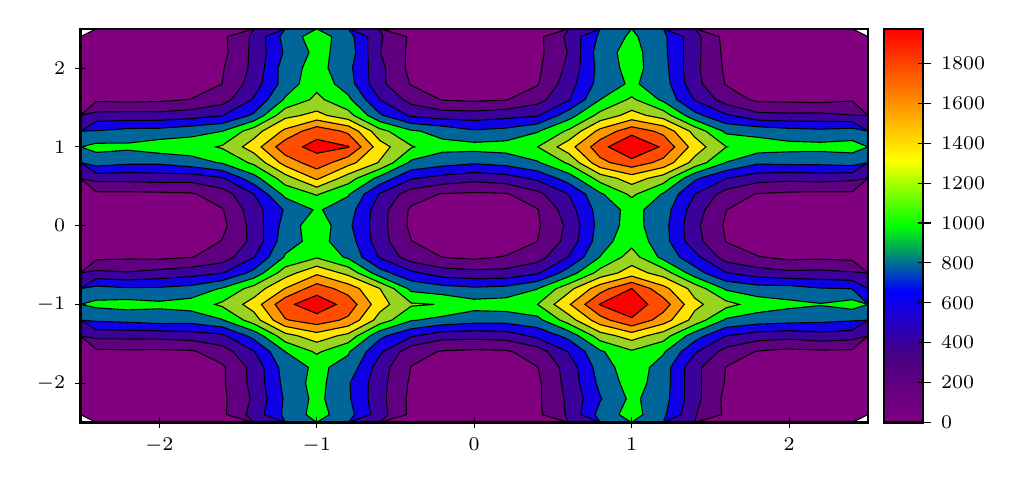
\begin{tikzpicture}
\begin{scope}[]
\pgfpointadd{\pgfpointxy {0.0} {0.0}} {\pgfpoint{0cm}{0cm}}\pgfpathmoveto{ NIL }
\pgfpointadd{\pgfpointxy {0.0} {0.0}} {\pgfpoint{10cm}{0cm}}\pgfpathlineto{ NIL }
\pgfpointadd{\pgfpointxy {0.0} {0.0}} {\pgfpoint{10cm}{5cm}}\pgfpathlineto{ NIL }
\pgfpointadd{\pgfpointxy {0.0} {0.0}} {\pgfpoint{0cm}{5cm}}\pgfpathlineto{ NIL }
\pgfpathclose
\pgfusepath{  clip, }
\begin{scope}[shift={(0.0,0.0)}]
\pgfsetxvec{\pgfpoint{2.0cm}{0cm}}
\pgfsetyvec{\pgfpoint{0cm}{1.0cm}}
\begin{scope}[shift={(2.5,2.5)}]
\begin{scope}[draw=black,fill=Indigo!0!violet]
\pgfpathmoveto{ \pgfpointxy {-2.5} {-2.4}}
\pgfpathlineto{ \pgfpointxy {-2.5} {-2.4}}
\pgfpathlineto{ \pgfpointxy {-2.5} {-2.2}}
\pgfpathlineto{ \pgfpointxy {-2.5} {-2.0}}
\pgfpathlineto{ \pgfpointxy {-2.5} {-1.8}}
\pgfpathlineto{ \pgfpointxy {-2.5} {-1.5999999}}
\pgfpathlineto{ \pgfpointxy {-2.5} {-1.4}}
\pgfpathlineto{ \pgfpointxy {-2.5} {-1.1999999}}
\pgfpathlineto{ \pgfpointxy {-2.5} {-1.0}}
\pgfpathlineto{ \pgfpointxy {-2.5} {-0.79999995}}
\pgfpathlineto{ \pgfpointxy {-2.5} {-0.6}}
\pgfpathlineto{ \pgfpointxy {-2.5} {-0.39999986}}
\pgfpathlineto{ \pgfpointxy {-2.5} {-0.20000005}}
\pgfpathlineto{ \pgfpointxy {-2.5} {0.0}}
\pgfpathlineto{ \pgfpointxy {-2.5} {0.20000005}}
\pgfpathlineto{ \pgfpointxy {-2.5} {0.4000001}}
\pgfpathlineto{ \pgfpointxy {-2.5} {0.60000014}}
\pgfpathlineto{ \pgfpointxy {-2.5} {0.79999995}}
\pgfpathlineto{ \pgfpointxy {-2.5} {1.0}}
\pgfpathlineto{ \pgfpointxy {-2.5} {1.2}}
\pgfpathlineto{ \pgfpointxy {-2.5} {1.4000001}}
\pgfpathlineto{ \pgfpointxy {-2.5} {1.5999999}}
\pgfpathlineto{ \pgfpointxy {-2.5} {1.8000002}}
\pgfpathlineto{ \pgfpointxy {-2.5} {2.0}}
\pgfpathlineto{ \pgfpointxy {-2.5} {2.2000003}}
\pgfpathlineto{ \pgfpointxy {-2.5} {2.4}}
\pgfpathlineto{ \pgfpointxy {-2.4} {2.5}}
\pgfpathlineto{ \pgfpointxy {-2.2} {2.5}}
\pgfpathlineto{ \pgfpointxy {-2.0} {2.5}}
\pgfpathlineto{ \pgfpointxy {-1.8} {2.5}}
\pgfpathlineto{ \pgfpointxy {-1.5999999} {2.5}}
\pgfpathlineto{ \pgfpointxy {-1.4} {2.5}}
\pgfpathlineto{ \pgfpointxy {-1.1999999} {2.5}}
\pgfpathlineto{ \pgfpointxy {-1.0} {2.5}}
\pgfpathlineto{ \pgfpointxy {-0.79999995} {2.5}}
\pgfpathlineto{ \pgfpointxy {-0.6} {2.5}}
\pgfpathlineto{ \pgfpointxy {-0.39999986} {2.5}}
\pgfpathlineto{ \pgfpointxy {-0.20000005} {2.5}}
\pgfpathlineto{ \pgfpointxy {0.0} {2.5}}
\pgfpathlineto{ \pgfpointxy {0.20000005} {2.5}}
\pgfpathlineto{ \pgfpointxy {0.4000001} {2.5}}
\pgfpathlineto{ \pgfpointxy {0.60000014} {2.5}}
\pgfpathlineto{ \pgfpointxy {0.79999995} {2.5}}
\pgfpathlineto{ \pgfpointxy {1.0} {2.5}}
\pgfpathlineto{ \pgfpointxy {1.2} {2.5}}
\pgfpathlineto{ \pgfpointxy {1.4000001} {2.5}}
\pgfpathlineto{ \pgfpointxy {1.5999999} {2.5}}
\pgfpathlineto{ \pgfpointxy {1.8000002} {2.5}}
\pgfpathlineto{ \pgfpointxy {2.0} {2.5}}
\pgfpathlineto{ \pgfpointxy {2.2000003} {2.5}}
\pgfpathlineto{ \pgfpointxy {2.4} {2.5}}
\pgfpathlineto{ \pgfpointxy {2.5} {2.4}}
\pgfpathlineto{ \pgfpointxy {2.5} {2.2000003}}
\pgfpathlineto{ \pgfpointxy {2.5} {2.0}}
\pgfpathlineto{ \pgfpointxy {2.5} {1.8000002}}
\pgfpathlineto{ \pgfpointxy {2.5} {1.5999999}}
\pgfpathlineto{ \pgfpointxy {2.5} {1.4000001}}
\pgfpathlineto{ \pgfpointxy {2.5} {1.2}}
\pgfpathlineto{ \pgfpointxy {2.5} {1.0}}
\pgfpathlineto{ \pgfpointxy {2.5} {0.79999995}}
\pgfpathlineto{ \pgfpointxy {2.5} {0.60000014}}
\pgfpathlineto{ \pgfpointxy {2.5} {0.4000001}}
\pgfpathlineto{ \pgfpointxy {2.5} {0.20000005}}
\pgfpathlineto{ \pgfpointxy {2.5} {0.0}}
\pgfpathlineto{ \pgfpointxy {2.5} {-0.20000005}}
\pgfpathlineto{ \pgfpointxy {2.5} {-0.39999986}}
\pgfpathlineto{ \pgfpointxy {2.5} {-0.6}}
\pgfpathlineto{ \pgfpointxy {2.5} {-0.79999995}}
\pgfpathlineto{ \pgfpointxy {2.5} {-1.0}}
\pgfpathlineto{ \pgfpointxy {2.5} {-1.1999999}}
\pgfpathlineto{ \pgfpointxy {2.5} {-1.4}}
\pgfpathlineto{ \pgfpointxy {2.5} {-1.5999999}}
\pgfpathlineto{ \pgfpointxy {2.5} {-1.8}}
\pgfpathlineto{ \pgfpointxy {2.5} {-2.0}}
\pgfpathlineto{ \pgfpointxy {2.5} {-2.2}}
\pgfpathlineto{ \pgfpointxy {2.5} {-2.4}}
\pgfpathlineto{ \pgfpointxy {2.4} {-2.5}}
\pgfpathlineto{ \pgfpointxy {2.2000003} {-2.5}}
\pgfpathlineto{ \pgfpointxy {2.0} {-2.5}}
\pgfpathlineto{ \pgfpointxy {1.8000002} {-2.5}}
\pgfpathlineto{ \pgfpointxy {1.5999999} {-2.5}}
\pgfpathlineto{ \pgfpointxy {1.4000001} {-2.5}}
\pgfpathlineto{ \pgfpointxy {1.2} {-2.5}}
\pgfpathlineto{ \pgfpointxy {1.0} {-2.5}}
\pgfpathlineto{ \pgfpointxy {0.79999995} {-2.5}}
\pgfpathlineto{ \pgfpointxy {0.60000014} {-2.5}}
\pgfpathlineto{ \pgfpointxy {0.4000001} {-2.5}}
\pgfpathlineto{ \pgfpointxy {0.20000005} {-2.5}}
\pgfpathlineto{ \pgfpointxy {0.0} {-2.5}}
\pgfpathlineto{ \pgfpointxy {-0.20000005} {-2.5}}
\pgfpathlineto{ \pgfpointxy {-0.39999986} {-2.5}}
\pgfpathlineto{ \pgfpointxy {-0.6} {-2.5}}
\pgfpathlineto{ \pgfpointxy {-0.79999995} {-2.5}}
\pgfpathlineto{ \pgfpointxy {-1.0} {-2.5}}
\pgfpathlineto{ \pgfpointxy {-1.1999999} {-2.5}}
\pgfpathlineto{ \pgfpointxy {-1.4} {-2.5}}
\pgfpathlineto{ \pgfpointxy {-1.5999999} {-2.5}}
\pgfpathlineto{ \pgfpointxy {-1.8} {-2.5}}
\pgfpathlineto{ \pgfpointxy {-2.0} {-2.5}}
\pgfpathlineto{ \pgfpointxy {-2.2} {-2.5}}
\pgfpathlineto{ \pgfpointxy {-2.4} {-2.5}}
\pgfpathclose
\pgfusepath{ stroke, fill, }
\end{scope}
\begin{scope}[draw=black,fill=Indigo!60!violet]
\pgfpathmoveto{ \pgfpointxy {-2.5} {-1.4}}
\pgfpathlineto{ \pgfpointxy {-2.5} {-1.4}}
\pgfpathlineto{ \pgfpointxy {-2.5} {-1.1999999}}
\pgfpathlineto{ \pgfpointxy {-2.5} {-1.0}}
\pgfpathlineto{ \pgfpointxy {-2.5} {-0.79999995}}
\pgfpathlineto{ \pgfpointxy {-2.5} {-0.6}}
\pgfpathlineto{ \pgfpointxy {-2.4} {-0.4343150341357678}}
\pgfpathlineto{ \pgfpointxy {-2.2} {-0.4233194667966531}}
\pgfpathlineto{ \pgfpointxy {-2.0} {-0.4267332989583412}}
\pgfpathlineto{ \pgfpointxy {-1.8} {-0.40563464048108067}}
\pgfpathlineto{ \pgfpointxy {-1.7816161614596244} {-0.39999986}}
\pgfpathlineto{ \pgfpointxy {-1.6140157430519269} {-0.20000005}}
\pgfpathlineto{ \pgfpointxy {-1.5999999} {-0.17033328121403812}}
\pgfpathlineto{ \pgfpointxy {-1.5682608589243077} {0.0}}
\pgfpathlineto{ \pgfpointxy {-1.5923174501070902} {0.20000005}}
\pgfpathlineto{ \pgfpointxy {-1.5999999} {0.2218018329519409}}
\pgfpathlineto{ \pgfpointxy {-1.7608130056053644} {0.4000001}}
\pgfpathlineto{ \pgfpointxy {-1.8} {0.41633902296777503}}
\pgfpathlineto{ \pgfpointxy {-2.0} {0.4250625403234731}}
\pgfpathlineto{ \pgfpointxy {-2.2} {0.43048547718131447}}
\pgfpathlineto{ \pgfpointxy {-2.4} {0.4309868823452607}}
\pgfpathlineto{ \pgfpointxy {-2.5} {0.60000014}}
\pgfpathlineto{ \pgfpointxy {-2.5} {0.79999995}}
\pgfpathlineto{ \pgfpointxy {-2.5} {1.0}}
\pgfpathlineto{ \pgfpointxy {-2.5} {1.2}}
\pgfpathlineto{ \pgfpointxy {-2.5} {1.4000001}}
\pgfpathlineto{ \pgfpointxy {-2.4} {1.5759333975503846}}
\pgfpathlineto{ \pgfpointxy {-2.2} {1.5677204285294817}}
\pgfpathlineto{ \pgfpointxy {-2.0} {1.5751792172209056}}
\pgfpathlineto{ \pgfpointxy {-1.8227907118686413} {1.5999999}}
\pgfpathlineto{ \pgfpointxy {-1.8} {1.607424311540795}}
\pgfpathlineto{ \pgfpointxy {-1.6014062447682955} {1.8000002}}
\pgfpathlineto{ \pgfpointxy {-1.5999999} {1.8112501295097179}}
\pgfpathlineto{ \pgfpointxy {-1.5883846058169238} {2.0}}
\pgfpathlineto{ \pgfpointxy {-1.562557366504044} {2.2000003}}
\pgfpathlineto{ \pgfpointxy {-1.569103932523813} {2.4}}
\pgfpathlineto{ \pgfpointxy {-1.4} {2.5}}
\pgfpathlineto{ \pgfpointxy {-1.1999999} {2.5}}
\pgfpathlineto{ \pgfpointxy {-1.0} {2.5}}
\pgfpathlineto{ \pgfpointxy {-0.79999995} {2.5}}
\pgfpathlineto{ \pgfpointxy {-0.6} {2.5}}
\pgfpathlineto{ \pgfpointxy {-0.4279844612010226} {2.4}}
\pgfpathlineto{ \pgfpointxy {-0.4368799650800228} {2.2000003}}
\pgfpathlineto{ \pgfpointxy {-0.4381586961197472} {2.0}}
\pgfpathlineto{ \pgfpointxy {-0.4099619420716971} {1.8000002}}
\pgfpathlineto{ \pgfpointxy {-0.39999986} {1.7814185109206129}}
\pgfpathlineto{ \pgfpointxy {-0.2159711814741434} {1.5999999}}
\pgfpathlineto{ \pgfpointxy {-0.20000005} {1.592768794030242}}
\pgfpathlineto{ \pgfpointxy {0.0} {1.5787539581123546}}
\pgfpathlineto{ \pgfpointxy {0.20000005} {1.5940413620215255}}
\pgfpathlineto{ \pgfpointxy {0.2150746595303512} {1.5999999}}
\pgfpathlineto{ \pgfpointxy {0.4000001} {1.7757447519708185}}
\pgfpathlineto{ \pgfpointxy {0.4104908377124121} {1.8000002}}
\pgfpathlineto{ \pgfpointxy {0.42854170667938885} {2.0}}
\pgfpathlineto{ \pgfpointxy {0.4433582489181367} {2.2000003}}
\pgfpathlineto{ \pgfpointxy {0.4399346809186575} {2.4}}
\pgfpathlineto{ \pgfpointxy {0.60000014} {2.5}}
\pgfpathlineto{ \pgfpointxy {0.79999995} {2.5}}
\pgfpathlineto{ \pgfpointxy {1.0} {2.5}}
\pgfpathlineto{ \pgfpointxy {1.2} {2.5}}
\pgfpathlineto{ \pgfpointxy {1.4000001} {2.5}}
\pgfpathlineto{ \pgfpointxy {1.5570833968965427} {2.4}}
\pgfpathlineto{ \pgfpointxy {1.5656508575488655} {2.2000003}}
\pgfpathlineto{ \pgfpointxy {1.5754676903848601} {2.0}}
\pgfpathlineto{ \pgfpointxy {1.5912636026406544} {1.8000002}}
\pgfpathlineto{ \pgfpointxy {1.5999999} {1.7794915980428962}}
\pgfpathlineto{ \pgfpointxy {1.745068563559693} {1.5999999}}
\pgfpathlineto{ \pgfpointxy {1.8000002} {1.5726280505990813}}
\pgfpathlineto{ \pgfpointxy {2.0} {1.5676491870838296}}
\pgfpathlineto{ \pgfpointxy {2.2000003} {1.5616502289862524}}
\pgfpathlineto{ \pgfpointxy {2.4} {1.5827149976891093}}
\pgfpathlineto{ \pgfpointxy {2.5} {1.4000001}}
\pgfpathlineto{ \pgfpointxy {2.5} {1.2}}
\pgfpathlineto{ \pgfpointxy {2.5} {1.0}}
\pgfpathlineto{ \pgfpointxy {2.5} {0.79999995}}
\pgfpathlineto{ \pgfpointxy {2.5} {0.60000014}}
\pgfpathlineto{ \pgfpointxy {2.4} {0.4306761965378323}}
\pgfpathlineto{ \pgfpointxy {2.2000003} {0.4301567802010662}}
\pgfpathlineto{ \pgfpointxy {2.0} {0.42664339660243566}}
\pgfpathlineto{ \pgfpointxy {1.8000002} {0.4084028174904071}}
\pgfpathlineto{ \pgfpointxy {1.7801640067652604} {0.4000001}}
\pgfpathlineto{ \pgfpointxy {1.60262075799087} {0.20000005}}
\pgfpathlineto{ \pgfpointxy {1.5999999} {0.1881250074226406}}
\pgfpathlineto{ \pgfpointxy {1.5781884703504439} {0.0}}
\pgfpathlineto{ \pgfpointxy {1.5962909739277586} {-0.20000005}}
\pgfpathlineto{ \pgfpointxy {1.5999999} {-0.20953266639018686}}
\pgfpathlineto{ \pgfpointxy {1.8000002} {-0.38279996148943907}}
\pgfpathlineto{ \pgfpointxy {1.8396923884245062} {-0.39999986}}
\pgfpathlineto{ \pgfpointxy {2.0} {-0.4355631056051612}}
\pgfpathlineto{ \pgfpointxy {2.2000003} {-0.42524472067718744}}
\pgfpathlineto{ \pgfpointxy {2.4} {-0.44066417210216446}}
\pgfpathlineto{ \pgfpointxy {2.5} {-0.6}}
\pgfpathlineto{ \pgfpointxy {2.5} {-0.79999995}}
\pgfpathlineto{ \pgfpointxy {2.5} {-1.0}}
\pgfpathlineto{ \pgfpointxy {2.5} {-1.1999999}}
\pgfpathlineto{ \pgfpointxy {2.5} {-1.4}}
\pgfpathlineto{ \pgfpointxy {2.4} {-1.574150932883879}}
\pgfpathlineto{ \pgfpointxy {2.2000003} {-1.5804022881482866}}
\pgfpathlineto{ \pgfpointxy {2.0} {-1.5652365824251144}}
\pgfpathlineto{ \pgfpointxy {1.8000002} {-1.5920914931517411}}
\pgfpathlineto{ \pgfpointxy {1.7819403701064305} {-1.5999999}}
\pgfpathlineto{ \pgfpointxy {1.5999999} {-1.7904687475855463}}
\pgfpathlineto{ \pgfpointxy {1.5953257355242396} {-1.8}}
\pgfpathlineto{ \pgfpointxy {1.5874265353348758} {-2.0}}
\pgfpathlineto{ \pgfpointxy {1.566392468961923} {-2.2}}
\pgfpathlineto{ \pgfpointxy {1.5702008680574382} {-2.4}}
\pgfpathlineto{ \pgfpointxy {1.4000001} {-2.5}}
\pgfpathlineto{ \pgfpointxy {1.2} {-2.5}}
\pgfpathlineto{ \pgfpointxy {1.0} {-2.5}}
\pgfpathlineto{ \pgfpointxy {0.79999995} {-2.5}}
\pgfpathlineto{ \pgfpointxy {0.60000014} {-2.5}}
\pgfpathlineto{ \pgfpointxy {0.4328000399047678} {-2.4}}
\pgfpathlineto{ \pgfpointxy {0.42688409780138636} {-2.2}}
\pgfpathlineto{ \pgfpointxy {0.4260390012498414} {-2.0}}
\pgfpathlineto{ \pgfpointxy {0.40350519431620535} {-1.8}}
\pgfpathlineto{ \pgfpointxy {0.4000001} {-1.7895918368046382}}
\pgfpathlineto{ \pgfpointxy {0.24516669887055942} {-1.5999999}}
\pgfpathlineto{ \pgfpointxy {0.20000005} {-1.5824025871198286}}
\pgfpathlineto{ \pgfpointxy {0.0} {-1.5746843750631294}}
\pgfpathlineto{ \pgfpointxy {-0.20000005} {-1.5894034988671017}}
\pgfpathlineto{ \pgfpointxy {-0.23552936573589545} {-1.5999999}}
\pgfpathlineto{ \pgfpointxy {-0.39999986} {-1.7839473714914762}}
\pgfpathlineto{ \pgfpointxy {-0.4040666319539148} {-1.8}}
\pgfpathlineto{ \pgfpointxy {-0.4212582437121708} {-2.0}}
\pgfpathlineto{ \pgfpointxy {-0.4325477365674866} {-2.2}}
\pgfpathlineto{ \pgfpointxy {-0.43027186932700623} {-2.4}}
\pgfpathlineto{ \pgfpointxy {-0.6} {-2.5}}
\pgfpathlineto{ \pgfpointxy {-0.79999995} {-2.5}}
\pgfpathlineto{ \pgfpointxy {-1.0} {-2.5}}
\pgfpathlineto{ \pgfpointxy {-1.1999999} {-2.5}}
\pgfpathlineto{ \pgfpointxy {-1.4} {-2.5}}
\pgfpathlineto{ \pgfpointxy {-1.5736050051432047} {-2.4}}
\pgfpathlineto{ \pgfpointxy {-1.5693283482374096} {-2.2}}
\pgfpathlineto{ \pgfpointxy {-1.5791695400649701} {-2.0}}
\pgfpathlineto{ \pgfpointxy {-1.5807534145359714} {-1.8}}
\pgfpathlineto{ \pgfpointxy {-1.5999999} {-1.7567692277271014}}
\pgfpathlineto{ \pgfpointxy {-1.7579844931622808} {-1.5999999}}
\pgfpathlineto{ \pgfpointxy {-1.8} {-1.5826836957375463}}
\pgfpathlineto{ \pgfpointxy {-2.0} {-1.5748474473811813}}
\pgfpathlineto{ \pgfpointxy {-2.2} {-1.5763194343064808}}
\pgfpathlineto{ \pgfpointxy {-2.4} {-1.569731533266354}}
\pgfpathclose
\pgfpathmoveto{ \pgfpointxy {-0.22568623038191404} {0.4000001}}
\pgfpathlineto{ \pgfpointxy {-0.22568623038191404} {0.4000001}}
\pgfpathlineto{ \pgfpointxy {-0.39999986} {0.2518333656365672}}
\pgfpathlineto{ \pgfpointxy {-0.4198721701401871} {0.20000005}}
\pgfpathlineto{ \pgfpointxy {-0.4275624658549204} {0.0}}
\pgfpathlineto{ \pgfpointxy {-0.39999986} {-0.17999994411760412}}
\pgfpathlineto{ \pgfpointxy {-0.39147822036950464} {-0.20000005}}
\pgfpathlineto{ \pgfpointxy {-0.20639170763418857} {-0.39999986}}
\pgfpathlineto{ \pgfpointxy {-0.20000005} {-0.40213054934318126}}
\pgfpathlineto{ \pgfpointxy {0.0} {-0.42691271728217206}}
\pgfpathlineto{ \pgfpointxy {0.14851853864612385} {-0.39999986}}
\pgfpathlineto{ \pgfpointxy {0.20000005} {-0.3817104878805968}}
\pgfpathlineto{ \pgfpointxy {0.4000001} {-0.2019468591698499}}
\pgfpathlineto{ \pgfpointxy {0.4008148541726446} {-0.20000005}}
\pgfpathlineto{ \pgfpointxy {0.41962409973032466} {0.0}}
\pgfpathlineto{ \pgfpointxy {0.4081875400720163} {0.20000005}}
\pgfpathlineto{ \pgfpointxy {0.4000001} {0.2172368757250278}}
\pgfpathlineto{ \pgfpointxy {0.2230573587660576} {0.4000001}}
\pgfpathlineto{ \pgfpointxy {0.20000005} {0.41117287966296256}}
\pgfpathlineto{ \pgfpointxy {0.0} {0.42075866061140754}}
\pgfpathlineto{ \pgfpointxy {-0.20000005} {0.40777452094264843}}
\pgfpathclose
\pgfusepath{ stroke, fill, }
\end{scope}
\begin{scope}[draw=black,fill=blue!20!Indigo]
\pgfpathmoveto{ \pgfpointxy {-2.5} {-1.4}}
\pgfpathlineto{ \pgfpointxy {-2.5} {-1.4}}
\pgfpathlineto{ \pgfpointxy {-2.5} {-1.1999999}}
\pgfpathlineto{ \pgfpointxy {-2.5} {-1.0}}
\pgfpathlineto{ \pgfpointxy {-2.5} {-0.79999995}}
\pgfpathlineto{ \pgfpointxy {-2.5} {-0.6}}
\pgfpathlineto{ \pgfpointxy {-2.4} {-0.5693150325711458}}
\pgfpathlineto{ \pgfpointxy {-2.2} {-0.586887929631219}}
\pgfpathlineto{ \pgfpointxy {-2.0} {-0.5581332974354425}}
\pgfpathlineto{ \pgfpointxy {-1.8} {-0.5276779827198745}}
\pgfpathlineto{ \pgfpointxy {-1.5999999} {-0.472677928812423}}
\pgfpathlineto{ \pgfpointxy {-1.5278114403568535} {-0.39999986}}
\pgfpathlineto{ \pgfpointxy {-1.4438174203137146} {-0.20000005}}
\pgfpathlineto{ \pgfpointxy {-1.44583850009471} {0.0}}
\pgfpathlineto{ \pgfpointxy {-1.4671745944146128} {0.20000005}}
\pgfpathlineto{ \pgfpointxy {-1.5327397187666534} {0.4000001}}
\pgfpathlineto{ \pgfpointxy {-1.5999999} {0.4727407773026715}}
\pgfpathlineto{ \pgfpointxy {-1.8} {0.5499661400631322}}
\pgfpathlineto{ \pgfpointxy {-2.0} {0.5482500388957559}}
\pgfpathlineto{ \pgfpointxy {-2.2} {0.5580582912367524}}
\pgfpathlineto{ \pgfpointxy {-2.4} {0.5606579334739794}}
\pgfpathlineto{ \pgfpointxy {-2.5} {0.60000014}}
\pgfpathlineto{ \pgfpointxy {-2.5} {0.79999995}}
\pgfpathlineto{ \pgfpointxy {-2.5} {1.0}}
\pgfpathlineto{ \pgfpointxy {-2.5} {1.2}}
\pgfpathlineto{ \pgfpointxy {-2.5} {1.4000001}}
\pgfpathlineto{ \pgfpointxy {-2.4} {1.4445333990732832}}
\pgfpathlineto{ \pgfpointxy {-2.2} {1.4479028007388117}}
\pgfpathlineto{ \pgfpointxy {-2.0} {1.4467753099142926}}
\pgfpathlineto{ \pgfpointxy {-1.8} {1.4727152979018676}}
\pgfpathlineto{ \pgfpointxy {-1.5999999} {1.5377618005592044}}
\pgfpathlineto{ \pgfpointxy {-1.5431023028650301} {1.5999999}}
\pgfpathlineto{ \pgfpointxy {-1.4656164300952057} {1.8000002}}
\pgfpathlineto{ \pgfpointxy {-1.4367692229587299} {2.0}}
\pgfpathlineto{ \pgfpointxy {-1.433311466362633} {2.2000003}}
\pgfpathlineto{ \pgfpointxy {-1.4278136115806932} {2.4}}
\pgfpathlineto{ \pgfpointxy {-1.4} {2.5}}
\pgfpathlineto{ \pgfpointxy {-1.1999999} {2.5}}
\pgfpathlineto{ \pgfpointxy {-1.0} {2.5}}
\pgfpathlineto{ \pgfpointxy {-0.79999995} {2.5}}
\pgfpathlineto{ \pgfpointxy {-0.6} {2.5}}
\pgfpathlineto{ \pgfpointxy {-0.5807751571046289} {2.4}}
\pgfpathlineto{ \pgfpointxy {-0.5945599632525442} {2.2000003}}
\pgfpathlineto{ \pgfpointxy {-0.5633015518122249} {2.0}}
\pgfpathlineto{ \pgfpointxy {-0.5598478718934856} {1.8000002}}
\pgfpathlineto{ \pgfpointxy {-0.45183516765020304} {1.5999999}}
\pgfpathlineto{ \pgfpointxy {-0.39999986} {1.5408547699935413}}
\pgfpathlineto{ \pgfpointxy {-0.20000005} {1.464364886723629}}
\pgfpathlineto{ \pgfpointxy {0.0} {1.4559502212178672}}
\pgfpathlineto{ \pgfpointxy {0.20000005} {1.4777581775285147}}
\pgfpathlineto{ \pgfpointxy {0.4000001} {1.5416733753194372}}
\pgfpathlineto{ \pgfpointxy {0.45696501648031784} {1.5999999}}
\pgfpathlineto{ \pgfpointxy {0.5314110817097446} {1.8000002}}
\pgfpathlineto{ \pgfpointxy {0.5654167050930359} {2.0}}
\pgfpathlineto{ \pgfpointxy {0.590447799452205} {2.2000003}}
\pgfpathlineto{ \pgfpointxy {0.5687582088373846} {2.4}}
\pgfpathlineto{ \pgfpointxy {0.60000014} {2.5}}
\pgfpathlineto{ \pgfpointxy {0.79999995} {2.5}}
\pgfpathlineto{ \pgfpointxy {1.0} {2.5}}
\pgfpathlineto{ \pgfpointxy {1.2} {2.5}}
\pgfpathlineto{ \pgfpointxy {1.4000001} {2.5}}
\pgfpathlineto{ \pgfpointxy {1.4397619696848452} {2.4}}
\pgfpathlineto{ \pgfpointxy {1.4405080018563878} {2.2000003}}
\pgfpathlineto{ \pgfpointxy {1.4336691308771967} {2.0}}
\pgfpathlineto{ \pgfpointxy {1.4489531349759242} {1.8000002}}
\pgfpathlineto{ \pgfpointxy {1.5339131111554485} {1.5999999}}
\pgfpathlineto{ \pgfpointxy {1.5999999} {1.5413505492515114}}
\pgfpathlineto{ \pgfpointxy {1.8000002} {1.4380888030116061}}
\pgfpathlineto{ \pgfpointxy {2.0} {1.429333399213197}}
\pgfpathlineto{ \pgfpointxy {2.2000003} {1.4315512205930827}}
\pgfpathlineto{ \pgfpointxy {2.4} {1.4043439590324107}}
\pgfpathlineto{ \pgfpointxy {2.5} {1.4000001}}
\pgfpathlineto{ \pgfpointxy {2.5} {1.2}}
\pgfpathlineto{ \pgfpointxy {2.5} {1.0}}
\pgfpathlineto{ \pgfpointxy {2.5} {0.79999995}}
\pgfpathlineto{ \pgfpointxy {2.5} {0.60000014}}
\pgfpathlineto{ \pgfpointxy {2.4} {0.5709608924208589}}
\pgfpathlineto{ \pgfpointxy {2.2000003} {0.5537304464804715}}
\pgfpathlineto{ \pgfpointxy {2.0} {0.5644755628371572}}
\pgfpathlineto{ \pgfpointxy {1.8000002} {0.5452778159040541}}
\pgfpathlineto{ \pgfpointxy {1.5999999} {0.46013796794209005}}
\pgfpathlineto{ \pgfpointxy {1.539021046509693} {0.4000001}}
\pgfpathlineto{ \pgfpointxy {1.4653793766354695} {0.20000005}}
\pgfpathlineto{ \pgfpointxy {1.4353623850492467} {0.0}}
\pgfpathlineto{ \pgfpointxy {1.4529455210436475} {-0.20000005}}
\pgfpathlineto{ \pgfpointxy {1.547257683822818} {-0.39999986}}
\pgfpathlineto{ \pgfpointxy {1.5999999} {-0.46346662935813265}}
\pgfpathlineto{ \pgfpointxy {1.8000002} {-0.5320429739420132}}
\pgfpathlineto{ \pgfpointxy {2.0} {-0.570102353192637}}
\pgfpathlineto{ \pgfpointxy {2.2000003} {-0.5630768869119089}}
\pgfpathlineto{ \pgfpointxy {2.4} {-0.5861254250288448}}
\pgfpathlineto{ \pgfpointxy {2.5} {-0.6}}
\pgfpathlineto{ \pgfpointxy {2.5} {-0.79999995}}
\pgfpathlineto{ \pgfpointxy {2.5} {-1.0}}
\pgfpathlineto{ \pgfpointxy {2.5} {-1.1999999}}
\pgfpathlineto{ \pgfpointxy {2.5} {-1.4}}
\pgfpathlineto{ \pgfpointxy {2.4} {-1.4501886701696325}}
\pgfpathlineto{ \pgfpointxy {2.2000003} {-1.467126427392165}}
\pgfpathlineto{ \pgfpointxy {2.0} {-1.4408832715635045}}
\pgfpathlineto{ \pgfpointxy {1.8000002} {-1.4632679652330145}}
\pgfpathlineto{ \pgfpointxy {1.5999999} {-1.5449084183268058}}
\pgfpathlineto{ \pgfpointxy {1.5495302686935304} {-1.5999999}}
\pgfpathlineto{ \pgfpointxy {1.4442912545160773} {-1.8}}
\pgfpathlineto{ \pgfpointxy {1.4425000664263088} {-2.0}}
\pgfpathlineto{ \pgfpointxy {1.4416456349646745} {-2.2}}
\pgfpathlineto{ \pgfpointxy {1.4118876168802084} {-2.4}}
\pgfpathlineto{ \pgfpointxy {1.4000001} {-2.5}}
\pgfpathlineto{ \pgfpointxy {1.2} {-2.5}}
\pgfpathlineto{ \pgfpointxy {1.0} {-2.5}}
\pgfpathlineto{ \pgfpointxy {0.79999995} {-2.5}}
\pgfpathlineto{ \pgfpointxy {0.60000014} {-2.5}}
\pgfpathlineto{ \pgfpointxy {0.5761454927888785} {-2.4}}
\pgfpathlineto{ \pgfpointxy {0.5697101831025835} {-2.2}}
\pgfpathlineto{ \pgfpointxy {0.5540260127535115} {-2.0}}
\pgfpathlineto{ \pgfpointxy {0.5389691102719798} {-1.8}}
\pgfpathlineto{ \pgfpointxy {0.46636946430251847} {-1.5999999}}
\pgfpathlineto{ \pgfpointxy {0.4000001} {-1.5406267722812812}}
\pgfpathlineto{ \pgfpointxy {0.20000005} {-1.4544155756161585}}
\pgfpathlineto{ \pgfpointxy {0.0} {-1.443720921431467}}
\pgfpathlineto{ \pgfpointxy {-0.20000005} {-1.451087710996469}}
\pgfpathlineto{ \pgfpointxy {-0.39999986} {-1.5266858704778923}}
\pgfpathlineto{ \pgfpointxy {-0.47047087809963584} {-1.5999999}}
\pgfpathlineto{ \pgfpointxy {-0.5354666304310163} {-1.8}}
\pgfpathlineto{ \pgfpointxy {-0.5517880435238611} {-2.0}}
\pgfpathlineto{ \pgfpointxy {-0.5580891363863731} {-2.2}}
\pgfpathlineto{ \pgfpointxy {-0.5493655235358592} {-2.4}}
\pgfpathlineto{ \pgfpointxy {-0.6} {-2.5}}
\pgfpathlineto{ \pgfpointxy {-0.79999995} {-2.5}}
\pgfpathlineto{ \pgfpointxy {-1.0} {-2.5}}
\pgfpathlineto{ \pgfpointxy {-1.1999999} {-2.5}}
\pgfpathlineto{ \pgfpointxy {-1.4} {-2.5}}
\pgfpathlineto{ \pgfpointxy {-1.4500313388637989} {-2.4}}
\pgfpathlineto{ \pgfpointxy {-1.422238797703341} {-2.2}}
\pgfpathlineto{ \pgfpointxy {-1.4427681575627889} {-2.0}}
\pgfpathlineto{ \pgfpointxy {-1.4457534161005934} {-1.8}}
\pgfpathlineto{ \pgfpointxy {-1.532241985894395} {-1.5999999}}
\pgfpathlineto{ \pgfpointxy {-1.5999999} {-1.5238399938082696}}
\pgfpathlineto{ \pgfpointxy {-1.8} {-1.4567412051844142}}
\pgfpathlineto{ \pgfpointxy {-2.0} {-1.441220330285824}}
\pgfpathlineto{ \pgfpointxy {-2.2} {-1.4394444358928338}}
\pgfpathlineto{ \pgfpointxy {-2.4} {-1.4374496556048426}}
\pgfpathclose
\pgfpathmoveto{ \pgfpointxy {-0.39999986} {-0.4601748906288825}}
\pgfpathlineto{ \pgfpointxy {-0.39999986} {-0.4601748906288825}}
\pgfpathlineto{ \pgfpointxy {-0.20000005} {-0.5375944652989557}}
\pgfpathlineto{ \pgfpointxy {0.0} {-0.5591945949436832}}
\pgfpathlineto{ \pgfpointxy {0.20000005} {-0.5471485568900185}}
\pgfpathlineto{ \pgfpointxy {0.4000001} {-0.46761900904632725}}
\pgfpathlineto{ \pgfpointxy {0.45875865757670864} {-0.39999986}}
\pgfpathlineto{ \pgfpointxy {0.546814852480535} {-0.20000005}}
\pgfpathlineto{ \pgfpointxy {0.5678195867345743} {0.0}}
\pgfpathlineto{ \pgfpointxy {0.531375038644299} {0.20000005}}
\pgfpathlineto{ \pgfpointxy {0.44511631486027703} {0.4000001}}
\pgfpathlineto{ \pgfpointxy {0.4000001} {0.4395918734341251}}
\pgfpathlineto{ \pgfpointxy {0.20000005} {0.532839544919538}}
\pgfpathlineto{ \pgfpointxy {0.0} {0.5566896935187535}}
\pgfpathlineto{ \pgfpointxy {-0.20000005} {0.5247478133554981}}
\pgfpathlineto{ \pgfpointxy {-0.39999986} {0.4672050066727289}}
\pgfpathlineto{ \pgfpointxy {-0.47462065227278316} {0.4000001}}
\pgfpathlineto{ \pgfpointxy {-0.5458146606933192} {0.20000005}}
\pgfpathlineto{ \pgfpointxy {-0.5507499644272027} {0.0}}
\pgfpathlineto{ \pgfpointxy {-0.538772526412449} {-0.20000005}}
\pgfpathlineto{ \pgfpointxy {-0.4724210150900636} {-0.39999986}}
\pgfpathclose
\pgfusepath{ stroke, fill, }
\end{scope}
\begin{scope}[draw=black,fill=blue!80!Indigo]
\pgfpathmoveto{ \pgfpointxy {-2.5} {-1.1999999}}
\pgfpathlineto{ \pgfpointxy {-2.5} {-1.1999999}}
\pgfpathlineto{ \pgfpointxy {-2.5} {-1.0}}
\pgfpathlineto{ \pgfpointxy {-2.5} {-0.79999995}}
\pgfpathlineto{ \pgfpointxy {-2.4} {-0.6733975555939846}}
\pgfpathlineto{ \pgfpointxy {-2.2} {-0.6901989702139031}}
\pgfpathlineto{ \pgfpointxy {-2.0} {-0.6741988591668682}}
\pgfpathlineto{ \pgfpointxy {-1.8} {-0.6464161482961535}}
\pgfpathlineto{ \pgfpointxy {-1.5999999} {-0.6044075472681161}}
\pgfpathlineto{ \pgfpointxy {-1.5929277550494265} {-0.6}}
\pgfpathlineto{ \pgfpointxy {-1.4} {-0.4055938265195751}}
\pgfpathlineto{ \pgfpointxy {-1.3965320575067381} {-0.39999986}}
\pgfpathlineto{ \pgfpointxy {-1.3379354732921047} {-0.20000005}}
\pgfpathlineto{ \pgfpointxy {-1.3377272633192216} {0.0}}
\pgfpathlineto{ \pgfpointxy {-1.3407142786110766} {0.20000005}}
\pgfpathlineto{ \pgfpointxy {-1.3985462459941531} {0.4000001}}
\pgfpathlineto{ \pgfpointxy {-1.4} {0.4020625334540382}}
\pgfpathlineto{ \pgfpointxy {-1.5852046738913534} {0.60000014}}
\pgfpathlineto{ \pgfpointxy {-1.5999999} {0.6115789865656356}}
\pgfpathlineto{ \pgfpointxy {-1.8} {0.6569515409618272}}
\pgfpathlineto{ \pgfpointxy {-2.0} {0.666069402285566}}
\pgfpathlineto{ \pgfpointxy {-2.2} {0.6720981313747019}}
\pgfpathlineto{ \pgfpointxy {-2.4} {0.6644601336968057}}
\pgfpathlineto{ \pgfpointxy {-2.5} {0.79999995}}
\pgfpathlineto{ \pgfpointxy {-2.5} {1.0}}
\pgfpathlineto{ \pgfpointxy {-2.5} {1.2}}
\pgfpathlineto{ \pgfpointxy {-2.4} {1.3228994745183624}}
\pgfpathlineto{ \pgfpointxy {-2.2} {1.3372414447995649}}
\pgfpathlineto{ \pgfpointxy {-2.0} {1.336717236799875}}
\pgfpathlineto{ \pgfpointxy {-1.8} {1.35792777587994}}
\pgfpathlineto{ \pgfpointxy {-1.5999999} {1.39684217118231}}
\pgfpathlineto{ \pgfpointxy {-1.5946610167332123} {1.4000001}}
\pgfpathlineto{ \pgfpointxy {-1.4130032944718605} {1.5999999}}
\pgfpathlineto{ \pgfpointxy {-1.4} {1.6325620709421225}}
\pgfpathlineto{ \pgfpointxy {-1.3473766143383918} {1.8000002}}
\pgfpathlineto{ \pgfpointxy {-1.3333482038941502} {2.0}}
\pgfpathlineto{ \pgfpointxy {-1.3209189098163232} {2.2000003}}
\pgfpathlineto{ \pgfpointxy {-1.3260280272093055} {2.4}}
\pgfpathlineto{ \pgfpointxy {-1.1999999} {2.5}}
\pgfpathlineto{ \pgfpointxy {-1.0} {2.5}}
\pgfpathlineto{ \pgfpointxy {-0.79999995} {2.5}}
\pgfpathlineto{ \pgfpointxy {-0.6762389039459218} {2.4}}
\pgfpathlineto{ \pgfpointxy {-0.6750690001578488} {2.2000003}}
\pgfpathlineto{ \pgfpointxy {-0.6716195019765498} {2.0}}
\pgfpathlineto{ \pgfpointxy {-0.666960522261407} {1.8000002}}
\pgfpathlineto{ \pgfpointxy {-0.6} {1.6009655999561838}}
\pgfpathlineto{ \pgfpointxy {-0.5994756153772829} {1.5999999}}
\pgfpathlineto{ \pgfpointxy {-0.42503871662787684} {1.4000001}}
\pgfpathlineto{ \pgfpointxy {-0.39999986} {1.3857395791665348}}
\pgfpathlineto{ \pgfpointxy {-0.20000005} {1.3542791344863039}}
\pgfpathlineto{ \pgfpointxy {0.0} {1.3353615123706772}}
\pgfpathlineto{ \pgfpointxy {0.20000005} {1.359815451770563}}
\pgfpathlineto{ \pgfpointxy {0.4000001} {1.3902525911329673}}
\pgfpathlineto{ \pgfpointxy {0.4118405245774728} {1.4000001}}
\pgfpathlineto{ \pgfpointxy {0.60000014} {1.591687570760958}}
\pgfpathlineto{ \pgfpointxy {0.6065196464554057} {1.5999999}}
\pgfpathlineto{ \pgfpointxy {0.6471271100648526} {1.8000002}}
\pgfpathlineto{ \pgfpointxy {0.6711594599766144} {2.0}}
\pgfpathlineto{ \pgfpointxy {0.6755328277846586} {2.2000003}}
\pgfpathlineto{ \pgfpointxy {0.6773575521835697} {2.4}}
\pgfpathlineto{ \pgfpointxy {0.79999995} {2.5}}
\pgfpathlineto{ \pgfpointxy {1.0} {2.5}}
\pgfpathlineto{ \pgfpointxy {1.2} {2.5}}
\pgfpathlineto{ \pgfpointxy {1.3295676330996526} {2.4}}
\pgfpathlineto{ \pgfpointxy {1.330026312013624} {2.2000003}}
\pgfpathlineto{ \pgfpointxy {1.3279137336178652} {2.0}}
\pgfpathlineto{ \pgfpointxy {1.3385748864933316} {1.8000002}}
\pgfpathlineto{ \pgfpointxy {1.3932787550985815} {1.5999999}}
\pgfpathlineto{ \pgfpointxy {1.4000001} {1.5909225817448096}}
\pgfpathlineto{ \pgfpointxy {1.5999999} {1.4145981391449838}}
\pgfpathlineto{ \pgfpointxy {1.6276830074390993} {1.4000001}}
\pgfpathlineto{ \pgfpointxy {1.8000002} {1.339744200356988}}
\pgfpathlineto{ \pgfpointxy {2.0} {1.3274299708948796}}
\pgfpathlineto{ \pgfpointxy {2.2000003} {1.3245960244980424}}
\pgfpathlineto{ \pgfpointxy {2.4} {1.319371132663211}}
\pgfpathlineto{ \pgfpointxy {2.5} {1.2}}
\pgfpathlineto{ \pgfpointxy {2.5} {1.0}}
\pgfpathlineto{ \pgfpointxy {2.5} {0.79999995}}
\pgfpathlineto{ \pgfpointxy {2.4} {0.6721940354152856}}
\pgfpathlineto{ \pgfpointxy {2.2000003} {0.6664690414352235}}
\pgfpathlineto{ \pgfpointxy {2.0} {0.6750256803043375}}
\pgfpathlineto{ \pgfpointxy {1.8000002} {0.6677937345023142}}
\pgfpathlineto{ \pgfpointxy {1.609193634883531} {0.60000014}}
\pgfpathlineto{ \pgfpointxy {1.5999999} {0.596069000849436}}
\pgfpathlineto{ \pgfpointxy {1.401188880274971} {0.4000001}}
\pgfpathlineto{ \pgfpointxy {1.4000001} {0.3967307822721504}}
\pgfpathlineto{ \pgfpointxy {1.3487218697133816} {0.20000005}}
\pgfpathlineto{ \pgfpointxy {1.3290431267529303} {0.0}}
\pgfpathlineto{ \pgfpointxy {1.3386173488858306} {-0.20000005}}
\pgfpathlineto{ \pgfpointxy {1.4000001} {-0.3288082415699338}}
\pgfpathlineto{ \pgfpointxy {1.4380610091881083} {-0.39999986}}
\pgfpathlineto{ \pgfpointxy {1.5999999} {-0.5948666278352337}}
\pgfpathlineto{ \pgfpointxy {1.614000089783561} {-0.6}}
\pgfpathlineto{ \pgfpointxy {1.8000002} {-0.6530051457086683}}
\pgfpathlineto{ \pgfpointxy {2.0} {-0.6706451268123315}}
\pgfpathlineto{ \pgfpointxy {2.2000003} {-0.6815253877816563}}
\pgfpathlineto{ \pgfpointxy {2.4} {-0.6958601797484261}}
\pgfpathlineto{ \pgfpointxy {2.5} {-0.79999995}}
\pgfpathlineto{ \pgfpointxy {2.5} {-1.0}}
\pgfpathlineto{ \pgfpointxy {2.5} {-1.1999999}}
\pgfpathlineto{ \pgfpointxy {2.4} {-1.329123859086786}}
\pgfpathlineto{ \pgfpointxy {2.2000003} {-1.3508868426102747}}
\pgfpathlineto{ \pgfpointxy {2.0} {-1.3341790948986119}}
\pgfpathlineto{ \pgfpointxy {1.8000002} {-1.3495979806788305}}
\pgfpathlineto{ \pgfpointxy {1.6013862307472992} {-1.4}}
\pgfpathlineto{ \pgfpointxy {1.5999999} {-1.4005128156047166}}
\pgfpathlineto{ \pgfpointxy {1.4172483910320195} {-1.5999999}}
\pgfpathlineto{ \pgfpointxy {1.4000001} {-1.6311515211914527}}
\pgfpathlineto{ \pgfpointxy {1.3365376497265422} {-1.8}}
\pgfpathlineto{ \pgfpointxy {1.3361009817789182} {-2.0}}
\pgfpathlineto{ \pgfpointxy {1.3359512843133472} {-2.2}}
\pgfpathlineto{ \pgfpointxy {1.3129833578508618} {-2.4}}
\pgfpathlineto{ \pgfpointxy {1.2} {-2.5}}
\pgfpathlineto{ \pgfpointxy {1.0} {-2.5}}
\pgfpathlineto{ \pgfpointxy {0.79999995} {-2.5}}
\pgfpathlineto{ \pgfpointxy {0.6760648548899701} {-2.4}}
\pgfpathlineto{ \pgfpointxy {0.6916224571965786} {-2.2}}
\pgfpathlineto{ \pgfpointxy {0.6682703090140949} {-2.0}}
\pgfpathlineto{ \pgfpointxy {0.6546970087944559} {-1.8}}
\pgfpathlineto{ \pgfpointxy {0.60000014} {-1.620991748330022}}
\pgfpathlineto{ \pgfpointxy {0.591910864121405} {-1.5999999}}
\pgfpathlineto{ \pgfpointxy {0.4000001} {-1.428319081275212}}
\pgfpathlineto{ \pgfpointxy {0.3390184279928907} {-1.4}}
\pgfpathlineto{ \pgfpointxy {0.20000005} {-1.341748062773658}}
\pgfpathlineto{ \pgfpointxy {0.0} {-1.3356372452300846}}
\pgfpathlineto{ \pgfpointxy {-0.20000005} {-1.3458387695834009}}
\pgfpathlineto{ \pgfpointxy {-0.36911559319415055} {-1.4}}
\pgfpathlineto{ \pgfpointxy {-0.39999986} {-1.413083566319015}}
\pgfpathlineto{ \pgfpointxy {-0.5796675527343458} {-1.5999999}}
\pgfpathlineto{ \pgfpointxy {-0.6} {-1.6535766525903761}}
\pgfpathlineto{ \pgfpointxy {-0.6466511278880196} {-1.8}}
\pgfpathlineto{ \pgfpointxy {-0.6726900220901995} {-2.0}}
\pgfpathlineto{ \pgfpointxy {-0.6737640089307273} {-2.2}}
\pgfpathlineto{ \pgfpointxy {-0.6587046276588822} {-2.4}}
\pgfpathlineto{ \pgfpointxy {-0.79999995} {-2.5}}
\pgfpathlineto{ \pgfpointxy {-1.0} {-2.5}}
\pgfpathlineto{ \pgfpointxy {-1.1999999} {-2.5}}
\pgfpathlineto{ \pgfpointxy {-1.3342857056906245} {-2.4}}
\pgfpathlineto{ \pgfpointxy {-1.3146428474715475} {-2.2}}
\pgfpathlineto{ \pgfpointxy {-1.3307928294644638} {-2.0}}
\pgfpathlineto{ \pgfpointxy {-1.3369007166462432} {-1.8}}
\pgfpathlineto{ \pgfpointxy {-1.394433488779027} {-1.5999999}}
\pgfpathlineto{ \pgfpointxy {-1.4} {-1.591567162332028}}
\pgfpathlineto{ \pgfpointxy {-1.5717056822637252} {-1.4}}
\pgfpathlineto{ \pgfpointxy {-1.5999999} {-1.3800941083305023}}
\pgfpathlineto{ \pgfpointxy {-1.8} {-1.3441752485831067}}
\pgfpathlineto{ \pgfpointxy {-2.0} {-1.336159240579717}}
\pgfpathlineto{ \pgfpointxy {-2.2} {-1.3280512726207576}}
\pgfpathlineto{ \pgfpointxy {-2.4} {-1.3227868762636772}}
\pgfpathclose
\pgfpathmoveto{ \pgfpointxy {-0.6} {-0.4105154220160747}}
\pgfpathlineto{ \pgfpointxy {-0.6} {-0.4105154220160747}}
\pgfpathlineto{ \pgfpointxy {-0.39999986} {-0.5751020029995251}}
\pgfpathlineto{ \pgfpointxy {-0.3426845105862455} {-0.6}}
\pgfpathlineto{ \pgfpointxy {-0.20000005} {-0.6555091027164581}}
\pgfpathlineto{ \pgfpointxy {0.0} {-0.6742778934136395}}
\pgfpathlineto{ \pgfpointxy {0.20000005} {-0.6673332979915998}}
\pgfpathlineto{ \pgfpointxy {0.4000001} {-0.614497572064542}}
\pgfpathlineto{ \pgfpointxy {0.418937533705495} {-0.6}}
\pgfpathlineto{ \pgfpointxy {0.5946896904840546} {-0.39999986}}
\pgfpathlineto{ \pgfpointxy {0.60000014} {-0.3884209976115618}}
\pgfpathlineto{ \pgfpointxy {0.6582791095438392} {-0.20000005}}
\pgfpathlineto{ \pgfpointxy {0.6719347718976314} {0.0}}
\pgfpathlineto{ \pgfpointxy {0.6469355223424014} {0.20000005}}
\pgfpathlineto{ \pgfpointxy {0.60000014} {0.39400000831484716}}
\pgfpathlineto{ \pgfpointxy {0.5979070107638838} {0.4000001}}
\pgfpathlineto{ \pgfpointxy {0.4000001} {0.573673504533208}}
\pgfpathlineto{ \pgfpointxy {0.3390551357475786} {0.60000014}}
\pgfpathlineto{ \pgfpointxy {0.20000005} {0.6500283666761333}}
\pgfpathlineto{ \pgfpointxy {0.0} {0.6752381337774231}}
\pgfpathlineto{ \pgfpointxy {-0.20000005} {0.6408721307188618}}
\pgfpathlineto{ \pgfpointxy {-0.3616091275283657} {0.60000014}}
\pgfpathlineto{ \pgfpointxy {-0.39999986} {0.5896273655023263}}
\pgfpathlineto{ \pgfpointxy {-0.6} {0.4088695994822875}}
\pgfpathlineto{ \pgfpointxy {-0.6071662408043683} {0.4000001}}
\pgfpathlineto{ \pgfpointxy {-0.6560099397722323} {0.20000005}}
\pgfpathlineto{ \pgfpointxy {-0.6660893493965683} {0.0}}
\pgfpathlineto{ \pgfpointxy {-0.6546471668261391} {-0.20000005}}
\pgfpathlineto{ \pgfpointxy {-0.6081382613494357} {-0.39999986}}
\pgfpathclose
\pgfusepath{ stroke, fill, }
\end{scope}
\begin{scope}[draw=black,fill=green!40!blue]
\pgfpathmoveto{ \pgfpointxy {-2.5} {-1.1999999}}
\pgfpathlineto{ \pgfpointxy {-2.5} {-1.1999999}}
\pgfpathlineto{ \pgfpointxy {-2.5} {-1.0}}
\pgfpathlineto{ \pgfpointxy {-2.5} {-0.79999995}}
\pgfpathlineto{ \pgfpointxy {-2.4} {-0.7683855063003229}}
\pgfpathlineto{ \pgfpointxy {-2.2} {-0.7882586705699488}}
\pgfpathlineto{ \pgfpointxy {-2.0} {-0.783093885529107}}
\pgfpathlineto{ \pgfpointxy {-1.8} {-0.7603467828138715}}
\pgfpathlineto{ \pgfpointxy {-1.5999999} {-0.6978198684603683}}
\pgfpathlineto{ \pgfpointxy {-1.443041825227638} {-0.6}}
\pgfpathlineto{ \pgfpointxy {-1.4} {-0.5566283075277374}}
\pgfpathlineto{ \pgfpointxy {-1.3028978543164047} {-0.39999986}}
\pgfpathlineto{ \pgfpointxy {-1.253161280726233} {-0.20000005}}
\pgfpathlineto{ \pgfpointxy {-1.2381818099274782} {0.0}}
\pgfpathlineto{ \pgfpointxy {-1.2127272671074063} {0.20000005}}
\pgfpathlineto{ \pgfpointxy {-1.3117180531678747} {0.4000001}}
\pgfpathlineto{ \pgfpointxy {-1.4} {0.5252500320263205}}
\pgfpathlineto{ \pgfpointxy {-1.4699415173324928} {0.60000014}}
\pgfpathlineto{ \pgfpointxy {-1.5999999} {0.7017849351769176}}
\pgfpathlineto{ \pgfpointxy {-1.8} {0.7479908008766776}}
\pgfpathlineto{ \pgfpointxy {-2.0} {0.7800000368032842}}
\pgfpathlineto{ \pgfpointxy {-2.2} {0.7795095742715152}}
\pgfpathlineto{ \pgfpointxy {-2.4} {0.7569953438919477}}
\pgfpathlineto{ \pgfpointxy {-2.5} {0.79999995}}
\pgfpathlineto{ \pgfpointxy {-2.5} {1.0}}
\pgfpathlineto{ \pgfpointxy {-2.5} {1.2}}
\pgfpathlineto{ \pgfpointxy {-2.4} {1.206272256935137}}
\pgfpathlineto{ \pgfpointxy {-2.2} {1.2326791117939142}}
\pgfpathlineto{ \pgfpointxy {-2.0} {1.2371717834081313}}
\pgfpathlineto{ \pgfpointxy {-1.8} {1.2629398251736026}}
\pgfpathlineto{ \pgfpointxy {-1.5999999} {1.2980451798461434}}
\pgfpathlineto{ \pgfpointxy {-1.4276271203640156} {1.4000001}}
\pgfpathlineto{ \pgfpointxy {-1.4} {1.4310476975157154}}
\pgfpathlineto{ \pgfpointxy {-1.3112999927297235} {1.5999999}}
\pgfpathlineto{ \pgfpointxy {-1.244987005135456} {1.8000002}}
\pgfpathlineto{ \pgfpointxy {-1.245357133485377} {2.0}}
\pgfpathlineto{ \pgfpointxy {-1.2143783705105655} {2.2000003}}
\pgfpathlineto{ \pgfpointxy {-1.23392522453844} {2.4}}
\pgfpathlineto{ \pgfpointxy {-1.1999999} {2.5}}
\pgfpathlineto{ \pgfpointxy {-1.0} {2.5}}
\pgfpathlineto{ \pgfpointxy {-0.79999995} {2.5}}
\pgfpathlineto{ \pgfpointxy {-0.7634512923156791} {2.4}}
\pgfpathlineto{ \pgfpointxy {-0.7528204785466666} {2.2000003}}
\pgfpathlineto{ \pgfpointxy {-0.7729562617275278} {2.0}}
\pgfpathlineto{ \pgfpointxy {-0.7584222381387395} {1.8000002}}
\pgfpathlineto{ \pgfpointxy {-0.6896803287841957} {1.5999999}}
\pgfpathlineto{ \pgfpointxy {-0.6} {1.4254222992804317}}
\pgfpathlineto{ \pgfpointxy {-0.5778294125314827} {1.4000001}}
\pgfpathlineto{ \pgfpointxy {-0.39999986} {1.2987197126254078}}
\pgfpathlineto{ \pgfpointxy {-0.20000005} {1.2626047169441397}}
\pgfpathlineto{ \pgfpointxy {0.0} {1.216626573987754}}
\pgfpathlineto{ \pgfpointxy {0.20000005} {1.2385231454840073}}
\pgfpathlineto{ \pgfpointxy {0.4000001} {1.290707137741224}}
\pgfpathlineto{ \pgfpointxy {0.5327607685748048} {1.4000001}}
\pgfpathlineto{ \pgfpointxy {0.60000014} {1.4685000721886756}}
\pgfpathlineto{ \pgfpointxy {0.7031372923944508} {1.5999999}}
\pgfpathlineto{ \pgfpointxy {0.7560221364270912} {1.8000002}}
\pgfpathlineto{ \pgfpointxy {0.7663768501774126} {2.0}}
\pgfpathlineto{ \pgfpointxy {0.75631151537304} {2.2000003}}
\pgfpathlineto{ \pgfpointxy {0.7794819033315763} {2.4}}
\pgfpathlineto{ \pgfpointxy {0.79999995} {2.5}}
\pgfpathlineto{ \pgfpointxy {1.0} {2.5}}
\pgfpathlineto{ \pgfpointxy {1.2} {2.5}}
\pgfpathlineto{ \pgfpointxy {1.2230270937938945} {2.4}}
\pgfpathlineto{ \pgfpointxy {1.2265617462836227} {2.2000003}}
\pgfpathlineto{ \pgfpointxy {1.2333813606127562} {2.0}}
\pgfpathlineto{ \pgfpointxy {1.2449406833029983} {1.8000002}}
\pgfpathlineto{ \pgfpointxy {1.2855738383140718} {1.5999999}}
\pgfpathlineto{ \pgfpointxy {1.4000001} {1.44546132881813}}
\pgfpathlineto{ \pgfpointxy {1.4522034664224774} {1.4000001}}
\pgfpathlineto{ \pgfpointxy {1.5999999} {1.2943030995004108}}
\pgfpathlineto{ \pgfpointxy {1.8000002} {1.2556930286232344}}
\pgfpathlineto{ \pgfpointxy {2.0} {1.2353271682240141}}
\pgfpathlineto{ \pgfpointxy {2.2000003} {1.2250505711062996}}
\pgfpathlineto{ \pgfpointxy {2.4} {1.236729624187047}}
\pgfpathlineto{ \pgfpointxy {2.5} {1.2}}
\pgfpathlineto{ \pgfpointxy {2.5} {1.0}}
\pgfpathlineto{ \pgfpointxy {2.5} {0.79999995}}
\pgfpathlineto{ \pgfpointxy {2.4} {0.7632332953301368}}
\pgfpathlineto{ \pgfpointxy {2.2000003} {0.7727224094760063}}
\pgfpathlineto{ \pgfpointxy {2.0} {0.7761026022098001}}
\pgfpathlineto{ \pgfpointxy {1.8000002} {0.7807450225915127}}
\pgfpathlineto{ \pgfpointxy {1.5999999} {0.700209460835806}}
\pgfpathlineto{ \pgfpointxy {1.4291072200531407} {0.60000014}}
\pgfpathlineto{ \pgfpointxy {1.4000001} {0.5714035362188228}}
\pgfpathlineto{ \pgfpointxy {1.2957867343672116} {0.4000001}}
\pgfpathlineto{ \pgfpointxy {1.2499248783772154} {0.20000005}}
\pgfpathlineto{ \pgfpointxy {1.2347369077502255} {0.0}}
\pgfpathlineto{ \pgfpointxy {1.2412840166805705} {-0.20000005}}
\pgfpathlineto{ \pgfpointxy {1.3038202970449846} {-0.39999986}}
\pgfpathlineto{ \pgfpointxy {1.4000001} {-0.5183409650465858}}
\pgfpathlineto{ \pgfpointxy {1.463741081284105} {-0.6}}
\pgfpathlineto{ \pgfpointxy {1.5999999} {-0.7061064041453915}}
\pgfpathlineto{ \pgfpointxy {1.8000002} {-0.7551294968566742}}
\pgfpathlineto{ \pgfpointxy {2.0} {-0.7614746188471941}}
\pgfpathlineto{ \pgfpointxy {2.2000003} {-0.7928813186944537}}
\pgfpathlineto{ \pgfpointxy {2.357500333450739} {-0.79999995}}
\pgfpathlineto{ \pgfpointxy {2.4} {-0.8023943261928119}}
\pgfpathlineto{ \pgfpointxy {2.5} {-1.0}}
\pgfpathlineto{ \pgfpointxy {2.5} {-1.1999999}}
\pgfpathlineto{ \pgfpointxy {2.4} {-1.2100302048779328}}
\pgfpathlineto{ \pgfpointxy {2.2000003} {-1.2303363852918332}}
\pgfpathlineto{ \pgfpointxy {2.0} {-1.2361193945425661}}
\pgfpathlineto{ \pgfpointxy {1.8000002} {-1.250552755696091}}
\pgfpathlineto{ \pgfpointxy {1.5999999} {-1.291491706237938}}
\pgfpathlineto{ \pgfpointxy {1.462175512293975} {-1.4}}
\pgfpathlineto{ \pgfpointxy {1.4000001} {-1.4681538468438846}}
\pgfpathlineto{ \pgfpointxy {1.3129949912776806} {-1.5999999}}
\pgfpathlineto{ \pgfpointxy {1.2467426621567688} {-1.8}}
\pgfpathlineto{ \pgfpointxy {1.2456881387900869} {-2.0}}
\pgfpathlineto{ \pgfpointxy {1.2398049439642493} {-2.2}}
\pgfpathlineto{ \pgfpointxy {1.2189022133565182} {-2.4}}
\pgfpathlineto{ \pgfpointxy {1.2} {-2.5}}
\pgfpathlineto{ \pgfpointxy {1.0} {-2.5}}
\pgfpathlineto{ \pgfpointxy {0.79999995} {-2.5}}
\pgfpathlineto{ \pgfpointxy {0.7673148538324011} {-2.4}}
\pgfpathlineto{ \pgfpointxy {0.79999995} {-2.231904708182527}}
\pgfpathlineto{ \pgfpointxy {0.8105098368712498} {-2.2}}
\pgfpathlineto{ \pgfpointxy {0.79999995} {-2.155333397815626}}
\pgfpathlineto{ \pgfpointxy {0.7748108483198521} {-2.0}}
\pgfpathlineto{ \pgfpointxy {0.7542424621861987} {-1.8}}
\pgfpathlineto{ \pgfpointxy {0.7041808269067666} {-1.5999999}}
\pgfpathlineto{ \pgfpointxy {0.60000014} {-1.448230454191995}}
\pgfpathlineto{ \pgfpointxy {0.5431068211851762} {-1.4}}
\pgfpathlineto{ \pgfpointxy {0.4000001} {-1.2947142826723204}}
\pgfpathlineto{ \pgfpointxy {0.20000005} {-1.2404113030226802}}
\pgfpathlineto{ \pgfpointxy {0.0} {-1.2390195992910396}}
\pgfpathlineto{ \pgfpointxy {-0.20000005} {-1.259956417637583}}
\pgfpathlineto{ \pgfpointxy {-0.39999986} {-1.309870794092808}}
\pgfpathlineto{ \pgfpointxy {-0.5571170693501695} {-1.4}}
\pgfpathlineto{ \pgfpointxy {-0.6} {-1.4457692351421487}}
\pgfpathlineto{ \pgfpointxy {-0.6850928000722387} {-1.5999999}}
\pgfpathlineto{ \pgfpointxy {-0.7383255454301831} {-1.8}}
\pgfpathlineto{ \pgfpointxy {-0.7879531786490601} {-2.0}}
\pgfpathlineto{ \pgfpointxy {-0.7844943447260373} {-2.2}}
\pgfpathlineto{ \pgfpointxy {-0.7608289788068883} {-2.4}}
\pgfpathlineto{ \pgfpointxy {-0.79999995} {-2.5}}
\pgfpathlineto{ \pgfpointxy {-1.0} {-2.5}}
\pgfpathlineto{ \pgfpointxy {-1.1999999} {-2.5}}
\pgfpathlineto{ \pgfpointxy {-1.2238655389031443} {-2.4}}
\pgfpathlineto{ \pgfpointxy {-1.2140816241472352} {-2.2}}
\pgfpathlineto{ \pgfpointxy {-1.2299744163106776} {-2.0}}
\pgfpathlineto{ \pgfpointxy {-1.241452775863845} {-1.8}}
\pgfpathlineto{ \pgfpointxy {-1.2973398938452083} {-1.5999999}}
\pgfpathlineto{ \pgfpointxy {-1.4} {-1.4444776117979592}}
\pgfpathlineto{ \pgfpointxy {-1.4398662189087743} {-1.4}}
\pgfpathlineto{ \pgfpointxy {-1.5999999} {-1.287341168229019}}
\pgfpathlineto{ \pgfpointxy {-1.8} {-1.242577311616276}}
\pgfpathlineto{ \pgfpointxy {-2.0} {-1.243840740478709}}
\pgfpathlineto{ \pgfpointxy {-2.2} {-1.226974350715295}}
\pgfpathlineto{ \pgfpointxy {-2.4} {-1.215081959479168}}
\pgfpathclose
\pgfpathmoveto{ \pgfpointxy {-0.5152715225751026} {0.60000014}}
\pgfpathlineto{ \pgfpointxy {-0.5152715225751026} {0.60000014}}
\pgfpathlineto{ \pgfpointxy {-0.6} {0.5231304677232451}}
\pgfpathlineto{ \pgfpointxy {-0.6994847409053764} {0.4000001}}
\pgfpathlineto{ \pgfpointxy {-0.7543141780344029} {0.20000005}}
\pgfpathlineto{ \pgfpointxy {-0.7762010799639714} {0.0}}
\pgfpathlineto{ \pgfpointxy {-0.7505595744736582} {-0.20000005}}
\pgfpathlineto{ \pgfpointxy {-0.7129786856662716} {-0.39999986}}
\pgfpathlineto{ \pgfpointxy {-0.6} {-0.5459793379718492}}
\pgfpathlineto{ \pgfpointxy {-0.5325321415962065} {-0.6}}
\pgfpathlineto{ \pgfpointxy {-0.39999986} {-0.7022516150091658}}
\pgfpathlineto{ \pgfpointxy {-0.20000005} {-0.7584333835079213}}
\pgfpathlineto{ \pgfpointxy {0.0} {-0.7816893363104527}}
\pgfpathlineto{ \pgfpointxy {0.20000005} {-0.7684102198970624}}
\pgfpathlineto{ \pgfpointxy {0.4000001} {-0.7088037910672464}}
\pgfpathlineto{ \pgfpointxy {0.5421250322777778} {-0.6}}
\pgfpathlineto{ \pgfpointxy {0.60000014} {-0.5343261970315418}}
\pgfpathlineto{ \pgfpointxy {0.696386805448975} {-0.39999986}}
\pgfpathlineto{ \pgfpointxy {0.7499535270860025} {-0.20000005}}
\pgfpathlineto{ \pgfpointxy {0.7638228827207798} {0.0}}
\pgfpathlineto{ \pgfpointxy {0.752903263049741} {0.20000005}}
\pgfpathlineto{ \pgfpointxy {0.7071074742990087} {0.4000001}}
\pgfpathlineto{ \pgfpointxy {0.60000014} {0.5369014389959856}}
\pgfpathlineto{ \pgfpointxy {0.5277419637576224} {0.60000014}}
\pgfpathlineto{ \pgfpointxy {0.4000001} {0.6951351702025343}}
\pgfpathlineto{ \pgfpointxy {0.20000005} {0.7616997534838679}}
\pgfpathlineto{ \pgfpointxy {0.0} {0.7856583005649034}}
\pgfpathlineto{ \pgfpointxy {-0.20000005} {0.7554651526465666}}
\pgfpathlineto{ \pgfpointxy {-0.39999986} {0.7070623499340756}}
\pgfpathclose
\pgfusepath{ stroke, fill, }
\end{scope}
\begin{scope}[draw=black,fill=yellow!0!green]
\pgfpathmoveto{ \pgfpointxy {-2.5} {-1.0}}
\pgfpathlineto{ \pgfpointxy {-2.5} {-1.0}}
\pgfpathlineto{ \pgfpointxy {-2.4} {-0.9469273219894425}}
\pgfpathlineto{ \pgfpointxy {-2.2} {-0.9376983686985947}}
\pgfpathlineto{ \pgfpointxy {-2.0} {-0.9608695170585657}}
\pgfpathlineto{ \pgfpointxy {-1.8} {-0.9223809040089443}}
\pgfpathlineto{ \pgfpointxy {-1.6251700905107322} {-0.79999995}}
\pgfpathlineto{ \pgfpointxy {-1.5999999} {-0.7912321896526202}}
\pgfpathlineto{ \pgfpointxy {-1.4} {-0.6670643993664469}}
\pgfpathlineto{ \pgfpointxy {-1.3369955100720508} {-0.6}}
\pgfpathlineto{ \pgfpointxy {-1.2092636511260713} {-0.39999986}}
\pgfpathlineto{ \pgfpointxy {-1.1999999} {-0.35806442806797545}}
\pgfpathlineto{ \pgfpointxy {-1.0919117821161366} {-0.20000005}}
\pgfpathlineto{ \pgfpointxy {-1.1035714284827316} {0.0}}
\pgfpathlineto{ \pgfpointxy {-1.0233830885507578} {0.20000005}}
\pgfpathlineto{ \pgfpointxy {-1.1999999} {0.35170942188964904}}
\pgfpathlineto{ \pgfpointxy {-1.2248898603415963} {0.4000001}}
\pgfpathlineto{ \pgfpointxy {-1.3589947058055454} {0.60000014}}
\pgfpathlineto{ \pgfpointxy {-1.4} {0.6490506633125905}}
\pgfpathlineto{ \pgfpointxy {-1.5999999} {0.7919908837882002}}
\pgfpathlineto{ \pgfpointxy {-1.6343137637803375} {0.79999995}}
\pgfpathlineto{ \pgfpointxy {-1.8} {0.8857868259782111}}
\pgfpathlineto{ \pgfpointxy {-2.0} {0.919047650869512}}
\pgfpathlineto{ \pgfpointxy {-2.2} {0.9579208177578917}}
\pgfpathlineto{ \pgfpointxy {-2.4} {0.9302469324642488}}
\pgfpathlineto{ \pgfpointxy {-2.5} {1.0}}
\pgfpathlineto{ \pgfpointxy {-2.4} {1.0465021319472743}}
\pgfpathlineto{ \pgfpointxy {-2.2} {1.047752891187923}}
\pgfpathlineto{ \pgfpointxy {-2.0} {1.0944445203193744}}
\pgfpathlineto{ \pgfpointxy {-1.8} {1.125698407219109}}
\pgfpathlineto{ \pgfpointxy {-1.5999999} {1.1986364424838265}}
\pgfpathlineto{ \pgfpointxy {-1.5990163971361568} {1.2}}
\pgfpathlineto{ \pgfpointxy {-1.4} {1.3297009229246117}}
\pgfpathlineto{ \pgfpointxy {-1.3345924383425571} {1.4000001}}
\pgfpathlineto{ \pgfpointxy {-1.2127499938718975} {1.5999999}}
\pgfpathlineto{ \pgfpointxy {-1.1999999} {1.6375001000459584}}
\pgfpathlineto{ \pgfpointxy {-1.1116000001966957} {1.8000002}}
\pgfpathlineto{ \pgfpointxy {-1.0914772814055063} {2.0}}
\pgfpathlineto{ \pgfpointxy {-1.0491150457313108} {2.2000003}}
\pgfpathlineto{ \pgfpointxy {-1.091266377354814} {2.4}}
\pgfpathlineto{ \pgfpointxy {-1.0} {2.5}}
\pgfpathlineto{ \pgfpointxy {-0.9045661624299877} {2.4}}
\pgfpathlineto{ \pgfpointxy {-0.9165412905296879} {2.2000003}}
\pgfpathlineto{ \pgfpointxy {-0.9284443978203663} {2.0}}
\pgfpathlineto{ \pgfpointxy {-0.8870444892389087} {1.8000002}}
\pgfpathlineto{ \pgfpointxy {-0.79999995} {1.658552727897309}}
\pgfpathlineto{ \pgfpointxy {-0.7796803277411144} {1.5999999}}
\pgfpathlineto{ \pgfpointxy {-0.6762443049022782} {1.4000001}}
\pgfpathlineto{ \pgfpointxy {-0.6} {1.3221709697062094}}
\pgfpathlineto{ \pgfpointxy {-0.39999986} {1.2116998460842812}}
\pgfpathlineto{ \pgfpointxy {-0.34044934735539156} {1.2}}
\pgfpathlineto{ \pgfpointxy {-0.20000005} {1.098374079809926}}
\pgfpathlineto{ \pgfpointxy {0.0} {1.058159070683324}}
\pgfpathlineto{ \pgfpointxy {0.20000005} {1.0766055818339555}}
\pgfpathlineto{ \pgfpointxy {0.4000001} {1.1833334130829294}}
\pgfpathlineto{ \pgfpointxy {0.41405624735307445} {1.2}}
\pgfpathlineto{ \pgfpointxy {0.60000014} {1.3451411394957091}}
\pgfpathlineto{ \pgfpointxy {0.6498575819183956} {1.4000001}}
\pgfpathlineto{ \pgfpointxy {0.7997549383334959} {1.5999999}}
\pgfpathlineto{ \pgfpointxy {0.79999995} {1.6008475629833798}}
\pgfpathlineto{ \pgfpointxy {0.9577181372866526} {1.8000002}}
\pgfpathlineto{ \pgfpointxy {0.9243902694597472} {2.0}}
\pgfpathlineto{ \pgfpointxy {0.907100611590069} {2.2000003}}
\pgfpathlineto{ \pgfpointxy {0.9607143106433202} {2.4}}
\pgfpathlineto{ \pgfpointxy {1.0} {2.5}}
\pgfpathlineto{ \pgfpointxy {1.0398964528592756} {2.4}}
\pgfpathlineto{ \pgfpointxy {1.0697778541776874} {2.2000003}}
\pgfpathlineto{ \pgfpointxy {1.0756098348483811} {2.0}}
\pgfpathlineto{ \pgfpointxy {1.0470150171932007} {1.8000002}}
\pgfpathlineto{ \pgfpointxy {1.170438029954251} {1.5999999}}
\pgfpathlineto{ \pgfpointxy {1.2} {1.5765218150097393}}
\pgfpathlineto{ \pgfpointxy {1.3384091599725867} {1.4000001}}
\pgfpathlineto{ \pgfpointxy {1.4000001} {1.3414687510249945}}
\pgfpathlineto{ \pgfpointxy {1.5775068499773823} {1.2}}
\pgfpathlineto{ \pgfpointxy {1.5999999} {1.1655602422616296}}
\pgfpathlineto{ \pgfpointxy {1.8000002} {1.1217647905647756}}
\pgfpathlineto{ \pgfpointxy {2.0} {1.0714286522732843}}
\pgfpathlineto{ \pgfpointxy {2.2000003} {1.058851752654788}}
\pgfpathlineto{ \pgfpointxy {2.4} {1.0803279507355619}}
\pgfpathlineto{ \pgfpointxy {2.5} {1.0}}
\pgfpathlineto{ \pgfpointxy {2.4} {0.9230366728848809}}
\pgfpathlineto{ \pgfpointxy {2.2000003} {0.9408654107855488}}
\pgfpathlineto{ \pgfpointxy {2.0} {0.9380734217754738}}
\pgfpathlineto{ \pgfpointxy {1.8000002} {0.9224719415554836}}
\pgfpathlineto{ \pgfpointxy {1.5999999} {0.8063107035330774}}
\pgfpathlineto{ \pgfpointxy {1.596024541834808} {0.79999995}}
\pgfpathlineto{ \pgfpointxy {1.4000001} {0.6678350879851074}}
\pgfpathlineto{ \pgfpointxy {1.3289417529981544} {0.60000014}}
\pgfpathlineto{ \pgfpointxy {1.2} {0.4110759762221874}}
\pgfpathlineto{ \pgfpointxy {1.1862205479264727} {0.4000001}}
\pgfpathlineto{ \pgfpointxy {1.076582364822868} {0.20000005}}
\pgfpathlineto{ \pgfpointxy {1.0767327524131485} {0.0}}
\pgfpathlineto{ \pgfpointxy {1.10734701384087} {-0.20000005}}
\pgfpathlineto{ \pgfpointxy {1.1659884418988993} {-0.39999986}}
\pgfpathlineto{ \pgfpointxy {1.2} {-0.4322313597625933}}
\pgfpathlineto{ \pgfpointxy {1.3474576970927656} {-0.6}}
\pgfpathlineto{ \pgfpointxy {1.4000001} {-0.6508196323481876}}
\pgfpathlineto{ \pgfpointxy {1.583046052857548} {-0.79999995}}
\pgfpathlineto{ \pgfpointxy {1.5999999} {-0.820274871116651}}
\pgfpathlineto{ \pgfpointxy {1.8000002} {-0.901843270096361}}
\pgfpathlineto{ \pgfpointxy {2.0} {-0.9427672395541227}}
\pgfpathlineto{ \pgfpointxy {2.2000003} {-0.9882652569562194}}
\pgfpathlineto{ \pgfpointxy {2.4} {-0.9411971414855247}}
\pgfpathlineto{ \pgfpointxy {2.5} {-1.0}}
\pgfpathlineto{ \pgfpointxy {2.4} {-1.0632575741263504}}
\pgfpathlineto{ \pgfpointxy {2.2000003} {-1.014465419507627}}
\pgfpathlineto{ \pgfpointxy {2.0} {-1.0535294209245376}}
\pgfpathlineto{ \pgfpointxy {1.8000002} {-1.1049261133071828}}
\pgfpathlineto{ \pgfpointxy {1.5999999} {-1.1784982916438134}}
\pgfpathlineto{ \pgfpointxy {1.582153050124477} {-1.1999999}}
\pgfpathlineto{ \pgfpointxy {1.4000001} {-1.349534878720378}}
\pgfpathlineto{ \pgfpointxy {1.3453401208299232} {-1.4}}
\pgfpathlineto{ \pgfpointxy {1.2129442310159284} {-1.5999999}}
\pgfpathlineto{ \pgfpointxy {1.2} {-1.6425000307336455}}
\pgfpathlineto{ \pgfpointxy {1.1133028300872096} {-1.8}}
\pgfpathlineto{ \pgfpointxy {1.0962766771066064} {-2.0}}
\pgfpathlineto{ \pgfpointxy {1.0556250856164846} {-2.2}}
\pgfpathlineto{ \pgfpointxy {1.0703704450601417} {-2.4}}
\pgfpathlineto{ \pgfpointxy {1.0} {-2.5}}
\pgfpathlineto{ \pgfpointxy {0.9193396489645504} {-2.4}}
\pgfpathlineto{ \pgfpointxy {0.9650980703737222} {-2.2}}
\pgfpathlineto{ \pgfpointxy {0.924896294929674} {-2.0}}
\pgfpathlineto{ \pgfpointxy {0.8926087235043876} {-1.8}}
\pgfpathlineto{ \pgfpointxy {0.827777800994991} {-1.5999999}}
\pgfpathlineto{ \pgfpointxy {0.79999995} {-1.5832317095749628}}
\pgfpathlineto{ \pgfpointxy {0.6630979851261629} {-1.4}}
\pgfpathlineto{ \pgfpointxy {0.60000014} {-1.336613266923608}}
\pgfpathlineto{ \pgfpointxy {0.4355372194416267} {-1.1999999}}
\pgfpathlineto{ \pgfpointxy {0.4000001} {-1.150000000121289}}
\pgfpathlineto{ \pgfpointxy {0.20000005} {-1.090277780944275}}
\pgfpathlineto{ \pgfpointxy {0.0} {-1.0801020462978255}}
\pgfpathlineto{ \pgfpointxy {-0.20000005} {-1.152016129999632}}
\pgfpathlineto{ \pgfpointxy {-0.3586665651400871} {-1.1999999}}
\pgfpathlineto{ \pgfpointxy {-0.39999986} {-1.2080103301570706}}
\pgfpathlineto{ \pgfpointxy {-0.6} {-1.334999993990945}}
\pgfpathlineto{ \pgfpointxy {-0.6619047237047249} {-1.4}}
\pgfpathlineto{ \pgfpointxy {-0.7896551330778894} {-1.5999999}}
\pgfpathlineto{ \pgfpointxy {-0.79999995} {-1.6464286208684964}}
\pgfpathlineto{ \pgfpointxy {-0.9228570696285785} {-1.8}}
\pgfpathlineto{ \pgfpointxy {-0.940079321115026} {-2.0}}
\pgfpathlineto{ \pgfpointxy {-0.9493391609401951} {-2.2}}
\pgfpathlineto{ \pgfpointxy {-0.9208954728806193} {-2.4}}
\pgfpathlineto{ \pgfpointxy {-1.0} {-2.5}}
\pgfpathlineto{ \pgfpointxy {-1.067948718923025} {-2.4}}
\pgfpathlineto{ \pgfpointxy {-1.0506607943563213} {-2.2}}
\pgfpathlineto{ \pgfpointxy {-1.0705607507621577} {-2.0}}
\pgfpathlineto{ \pgfpointxy {-1.053289486477642} {-1.8}}
\pgfpathlineto{ \pgfpointxy {-1.1999999} {-1.6008928903644644}}
\pgfpathlineto{ \pgfpointxy {-1.2002462989113896} {-1.5999999}}
\pgfpathlineto{ \pgfpointxy {-1.3396929766165846} {-1.4}}
\pgfpathlineto{ \pgfpointxy {-1.4} {-1.33678160386524}}
\pgfpathlineto{ \pgfpointxy {-1.592556637679875} {-1.1999999}}
\pgfpathlineto{ \pgfpointxy {-1.5999999} {-1.1905737723788767}}
\pgfpathlineto{ \pgfpointxy {-1.8} {-1.0831632708332373}}
\pgfpathlineto{ \pgfpointxy {-2.0} {-1.0562500147459413}}
\pgfpathlineto{ \pgfpointxy {-2.2} {-1.0704035895555013}}
\pgfpathlineto{ \pgfpointxy {-2.4} {-1.04377880420553}}
\pgfpathclose
\pgfpathmoveto{ \pgfpointxy {-0.7918032410063842} {0.4000001}}
\pgfpathlineto{ \pgfpointxy {-0.7918032410063842} {0.4000001}}
\pgfpathlineto{ \pgfpointxy {-0.79999995} {0.37154471578636716}}
\pgfpathlineto{ \pgfpointxy {-0.963565828102503} {0.20000005}}
\pgfpathlineto{ \pgfpointxy {-0.9084210105946187} {0.0}}
\pgfpathlineto{ \pgfpointxy {-0.9208860193721096} {-0.20000005}}
\pgfpathlineto{ \pgfpointxy {-0.8317535048977454} {-0.39999986}}
\pgfpathlineto{ \pgfpointxy {-0.79999995} {-0.4181571363998944}}
\pgfpathlineto{ \pgfpointxy {-0.6522026041366715} {-0.6}}
\pgfpathlineto{ \pgfpointxy {-0.6} {-0.6459301948114189}}
\pgfpathlineto{ \pgfpointxy {-0.4221476083633884} {-0.79999995}}
\pgfpathlineto{ \pgfpointxy {-0.39999986} {-0.8366666225426724}}
\pgfpathlineto{ \pgfpointxy {-0.20000005} {-0.8767973443700203}}
\pgfpathlineto{ \pgfpointxy {0.0} {-0.9351239220477823}}
\pgfpathlineto{ \pgfpointxy {0.20000005} {-0.9163089668674016}}
\pgfpathlineto{ \pgfpointxy {0.4000001} {-0.8064999486580484}}
\pgfpathlineto{ \pgfpointxy {0.4038461816690022} {-0.79999995}}
\pgfpathlineto{ \pgfpointxy {0.60000014} {-0.6479357402429939}}
\pgfpathlineto{ \pgfpointxy {0.6557333664337794} {-0.6}}
\pgfpathlineto{ \pgfpointxy {0.7966921477979074} {-0.39999986}}
\pgfpathlineto{ \pgfpointxy {0.79999995} {-0.3864582474498688}}
\pgfpathlineto{ \pgfpointxy {0.880995501867786} {-0.20000005}}
\pgfpathlineto{ \pgfpointxy {0.9213198214315517} {0.0}}
\pgfpathlineto{ \pgfpointxy {0.9288235497912933} {0.20000005}}
\pgfpathlineto{ \pgfpointxy {0.82150946375334} {0.4000001}}
\pgfpathlineto{ \pgfpointxy {0.79999995} {0.4186274774080396}}
\pgfpathlineto{ \pgfpointxy {0.6558441893079063} {0.60000014}}
\pgfpathlineto{ \pgfpointxy {0.60000014} {0.6639881268454091}}
\pgfpathlineto{ \pgfpointxy {0.4179283095308506} {0.79999995}}
\pgfpathlineto{ \pgfpointxy {0.4000001} {0.8209302577584285}}
\pgfpathlineto{ \pgfpointxy {0.20000005} {0.9215962706037528}}
\pgfpathlineto{ \pgfpointxy {0.0} {0.9423236810814783}}
\pgfpathlineto{ \pgfpointxy {-0.20000005} {0.9331491935812961}}
\pgfpathlineto{ \pgfpointxy {-0.39999986} {0.831889792871991}}
\pgfpathlineto{ \pgfpointxy {-0.41937794693562935} {0.79999995}}
\pgfpathlineto{ \pgfpointxy {-0.6} {0.6291855551774415}}
\pgfpathlineto{ \pgfpointxy {-0.6362359126171702} {0.60000014}}
\pgfpathclose
\pgfusepath{ stroke, fill, }
\end{scope}
\begin{scope}[draw=black,fill=yellow!60!green]
\pgfpathmoveto{ \pgfpointxy {-1.6468874460004819} {-1.0}}
\pgfpathlineto{ \pgfpointxy {-1.6468874460004819} {-1.0}}
\pgfpathlineto{ \pgfpointxy {-1.5999999} {-0.9669158357270407}}
\pgfpathlineto{ \pgfpointxy {-1.462615393255766} {-0.79999995}}
\pgfpathlineto{ \pgfpointxy {-1.4} {-0.7611455438607917}}
\pgfpathlineto{ \pgfpointxy {-1.248609860872207} {-0.6}}
\pgfpathlineto{ \pgfpointxy {-1.1999999} {-0.524195752846194}}
\pgfpathlineto{ \pgfpointxy {-1.0} {-0.4104812355331555}}
\pgfpathlineto{ \pgfpointxy {-0.79999995} {-0.5249864034544482}}
\pgfpathlineto{ \pgfpointxy {-0.7390307969629502} {-0.6}}
\pgfpathlineto{ \pgfpointxy {-0.6} {-0.7223255427632218}}
\pgfpathlineto{ \pgfpointxy {-0.5103355268043959} {-0.79999995}}
\pgfpathlineto{ \pgfpointxy {-0.39999986} {-0.9826666208505628}}
\pgfpathlineto{ \pgfpointxy {-0.2537497707270058} {-1.0}}
\pgfpathlineto{ \pgfpointxy {-0.39999986} {-1.022829276845223}}
\pgfpathlineto{ \pgfpointxy {-0.52311859337051} {-1.1999999}}
\pgfpathlineto{ \pgfpointxy {-0.6} {-1.2493043428102268}}
\pgfpathlineto{ \pgfpointxy {-0.743519629591123} {-1.4}}
\pgfpathlineto{ \pgfpointxy {-0.79999995} {-1.4868789857493088}}
\pgfpathlineto{ \pgfpointxy {-0.9691428044949255} {-1.5999999}}
\pgfpathlineto{ \pgfpointxy {-1.0} {-1.6342857345371025}}
\pgfpathlineto{ \pgfpointxy {-1.0282969486622315} {-1.5999999}}
\pgfpathlineto{ \pgfpointxy {-1.1999999} {-1.4763522057075924}}
\pgfpathlineto{ \pgfpointxy {-1.253245609197439} {-1.4}}
\pgfpathlineto{ \pgfpointxy {-1.4} {-1.2461609152603426}}
\pgfpathlineto{ \pgfpointxy {-1.4649838236244368} {-1.1999999}}
\pgfpathlineto{ \pgfpointxy {-1.5999999} {-1.029016397202113}}
\pgfpathclose
\pgfpathmoveto{ \pgfpointxy {-1.6403774047910051} {1.0}}
\pgfpathlineto{ \pgfpointxy {-1.6403774047910051} {1.0}}
\pgfpathlineto{ \pgfpointxy {-1.5999999} {1.0194546263786881}}
\pgfpathlineto{ \pgfpointxy {-1.4697704969947458} {1.2}}
\pgfpathlineto{ \pgfpointxy {-1.4} {1.245470154670059}}
\pgfpathlineto{ \pgfpointxy {-1.2562226579387195} {1.4000001}}
\pgfpathlineto{ \pgfpointxy {-1.1999999} {1.490351517178571}}
\pgfpathlineto{ \pgfpointxy {-1.0440000067840927} {1.5999999}}
\pgfpathlineto{ \pgfpointxy {-1.0} {1.691320876282342}}
\pgfpathlineto{ \pgfpointxy {-0.9518407417781907} {1.5999999}}
\pgfpathlineto{ \pgfpointxy {-0.79999995} {1.4667249772993762}}
\pgfpathlineto{ \pgfpointxy {-0.7654298242306274} {1.4000001}}
\pgfpathlineto{ \pgfpointxy {-0.6} {1.231131709791359}}
\pgfpathlineto{ \pgfpointxy {-0.5433612890554071} {1.2}}
\pgfpathlineto{ \pgfpointxy {-0.39999986} {1.017540192873402}}
\pgfpathlineto{ \pgfpointxy {-0.37856201893948205} {1.0}}
\pgfpathlineto{ \pgfpointxy {-0.39999986} {0.9870866414669925}}
\pgfpathlineto{ \pgfpointxy {-0.5136841659383338} {0.79999995}}
\pgfpathlineto{ \pgfpointxy {-0.6} {0.7183710745057903}}
\pgfpathlineto{ \pgfpointxy {-0.7469662484124802} {0.60000014}}
\pgfpathlineto{ \pgfpointxy {-0.79999995} {0.5310949128104818}}
\pgfpathlineto{ \pgfpointxy {-0.9832652515537879} {0.4000001}}
\pgfpathlineto{ \pgfpointxy {-1.0} {0.38273685208433506}}
\pgfpathlineto{ \pgfpointxy {-1.0208917376133293} {0.4000001}}
\pgfpathlineto{ \pgfpointxy {-1.1999999} {0.5152459208911555}}
\pgfpathlineto{ \pgfpointxy {-1.2547089927284807} {0.60000014}}
\pgfpathlineto{ \pgfpointxy {-1.4} {0.7737974973098387}}
\pgfpathlineto{ \pgfpointxy {-1.4374660758667406} {0.79999995}}
\pgfpathlineto{ \pgfpointxy {-1.5999999} {0.9787064883261172}}
\pgfpathclose
\pgfpathmoveto{ \pgfpointxy {0.5441322595053464} {-1.1999999}}
\pgfpathlineto{ \pgfpointxy {0.5441322595053464} {-1.1999999}}
\pgfpathlineto{ \pgfpointxy {0.40192002653360337} {-1.0}}
\pgfpathlineto{ \pgfpointxy {0.5204733992522281} {-0.79999995}}
\pgfpathlineto{ \pgfpointxy {0.60000014} {-0.7383485832318251}}
\pgfpathlineto{ \pgfpointxy {0.7608533652154601} {-0.6}}
\pgfpathlineto{ \pgfpointxy {0.79999995} {-0.544393886519652}}
\pgfpathlineto{ \pgfpointxy {0.9366308531250573} {-0.39999986}}
\pgfpathlineto{ \pgfpointxy {1.0} {-0.28519473150565977}}
\pgfpathlineto{ \pgfpointxy {1.0513954199711946} {-0.39999986}}
\pgfpathlineto{ \pgfpointxy {1.2} {-0.5408263998263136}}
\pgfpathlineto{ \pgfpointxy {1.2520097563103674} {-0.6}}
\pgfpathlineto{ \pgfpointxy {1.4000001} {-0.7431381324491957}}
\pgfpathlineto{ \pgfpointxy {1.4697701921014268} {-0.79999995}}
\pgfpathlineto{ \pgfpointxy {1.5999999} {-0.9557387870724257}}
\pgfpathlineto{ \pgfpointxy {1.6830968769500343} {-1.0}}
\pgfpathlineto{ \pgfpointxy {1.5999999} {-1.0439590440563378}}
\pgfpathlineto{ \pgfpointxy {1.470481663316742} {-1.1999999}}
\pgfpathlineto{ \pgfpointxy {1.4000001} {-1.2578604611782143}}
\pgfpathlineto{ \pgfpointxy {1.2460454116532724} {-1.4}}
\pgfpathlineto{ \pgfpointxy {1.2} {-1.469505711890219}}
\pgfpathlineto{ \pgfpointxy {1.0} {-1.5831111173393237}}
\pgfpathlineto{ \pgfpointxy {0.79999995} {-1.4630487841385895}}
\pgfpathlineto{ \pgfpointxy {0.7528929726959364} {-1.4}}
\pgfpathlineto{ \pgfpointxy {0.60000014} {-1.2464073183123254}}
\pgfpathclose
\pgfpathmoveto{ \pgfpointxy {0.5749801005393382} {0.79999995}}
\pgfpathlineto{ \pgfpointxy {0.5749801005393382} {0.79999995}}
\pgfpathlineto{ \pgfpointxy {0.4028750236760823} {1.0}}
\pgfpathlineto{ \pgfpointxy {0.5723694985303052} {1.2}}
\pgfpathlineto{ \pgfpointxy {0.60000014} {1.2215674732163033}}
\pgfpathlineto{ \pgfpointxy {0.7621652729244652} {1.4000001}}
\pgfpathlineto{ \pgfpointxy {0.79999995} {1.4504943792686267}}
\pgfpathlineto{ \pgfpointxy {0.9687553896041896} {1.5999999}}
\pgfpathlineto{ \pgfpointxy {1.0} {1.6360396966102098}}
\pgfpathlineto{ \pgfpointxy {1.0265694184829721} {1.5999999}}
\pgfpathlineto{ \pgfpointxy {1.2} {1.4622609467687822}}
\pgfpathlineto{ \pgfpointxy {1.2488182519200177} {1.4000001}}
\pgfpathlineto{ \pgfpointxy {1.4000001} {1.2563283632428552}}
\pgfpathlineto{ \pgfpointxy {1.4706775829228285} {1.2}}
\pgfpathlineto{ \pgfpointxy {1.5999999} {1.0019917794270636}}
\pgfpathlineto{ \pgfpointxy {1.6050001264363534} {1.0}}
\pgfpathlineto{ \pgfpointxy {1.5999999} {0.9976699246162344}}
\pgfpathlineto{ \pgfpointxy {1.4754740845163665} {0.79999995}}
\pgfpathlineto{ \pgfpointxy {1.4000001} {0.749113437558572}}
\pgfpathlineto{ \pgfpointxy {1.2438013652160151} {0.60000014}}
\pgfpathlineto{ \pgfpointxy {1.2} {0.5358228102194356}}
\pgfpathlineto{ \pgfpointxy {1.0310236993314716} {0.4000001}}
\pgfpathlineto{ \pgfpointxy {1.0} {0.3552272796732452}}
\pgfpathlineto{ \pgfpointxy {0.9702641790104356} {0.4000001}}
\pgfpathlineto{ \pgfpointxy {0.79999995} {0.5474510053267663}}
\pgfpathlineto{ \pgfpointxy {0.7582337985108425} {0.60000014}}
\pgfpathlineto{ \pgfpointxy {0.60000014} {0.7813095540571067}}
\pgfpathclose
\pgfusepath{ stroke, fill, }
\end{scope}
\begin{scope}[draw=black,fill=orange!20!yellow]
\pgfpathmoveto{ \pgfpointxy {-1.4701204959383933} {-1.0}}
\pgfpathlineto{ \pgfpointxy {-1.4701204959383933} {-1.0}}
\pgfpathlineto{ \pgfpointxy {-1.4} {-0.9139900881404355}}
\pgfpathlineto{ \pgfpointxy {-1.3279127778925262} {-0.79999995}}
\pgfpathlineto{ \pgfpointxy {-1.1999999} {-0.6603400837777016}}
\pgfpathlineto{ \pgfpointxy {-1.1278861881307958} {-0.6}}
\pgfpathlineto{ \pgfpointxy {-1.0} {-0.5158823038302958}}
\pgfpathlineto{ \pgfpointxy {-0.8543517934875902} {-0.6}}
\pgfpathlineto{ \pgfpointxy {-0.79999995} {-0.6323415498283609}}
\pgfpathlineto{ \pgfpointxy {-0.6} {-0.798720890715025}}
\pgfpathlineto{ \pgfpointxy {-0.5985234452454034} {-0.79999995}}
\pgfpathlineto{ \pgfpointxy {-0.536771595509737} {-1.0}}
\pgfpathlineto{ \pgfpointxy {-0.6} {-1.0979268529484192}}
\pgfpathlineto{ \pgfpointxy {-0.6383944509069033} {-1.1999999}}
\pgfpathlineto{ \pgfpointxy {-0.79999995} {-1.3706053277467702}}
\pgfpathlineto{ \pgfpointxy {-0.8705813285691095} {-1.4}}
\pgfpathlineto{ \pgfpointxy {-1.0} {-1.480652185208772}}
\pgfpathlineto{ \pgfpointxy {-1.1190374516675823} {-1.4}}
\pgfpathlineto{ \pgfpointxy {-1.1999999} {-1.3666519815917848}}
\pgfpathlineto{ \pgfpointxy {-1.359284208917618} {-1.1999999}}
\pgfpathlineto{ \pgfpointxy {-1.4} {-1.094891323137867}}
\pgfpathclose
\pgfpathmoveto{ \pgfpointxy {-1.4717518361739437} {1.0}}
\pgfpathlineto{ \pgfpointxy {-1.4717518361739437} {1.0}}
\pgfpathlineto{ \pgfpointxy {-1.4} {1.1040212564020568}}
\pgfpathlineto{ \pgfpointxy {-1.3450303079711672} {1.2}}
\pgfpathlineto{ \pgfpointxy {-1.1999999} {1.362237370466782}}
\pgfpathlineto{ \pgfpointxy {-1.1014159730525153} {1.4000001}}
\pgfpathlineto{ \pgfpointxy {-1.0} {1.4556311623896794}}
\pgfpathlineto{ \pgfpointxy {-0.9356179131500499} {1.4000001}}
\pgfpathlineto{ \pgfpointxy {-0.79999995} {1.348964132005014}}
\pgfpathlineto{ \pgfpointxy {-0.6538173847098321} {1.2}}
\pgfpathlineto{ \pgfpointxy {-0.6} {1.0820909956951041}}
\pgfpathlineto{ \pgfpointxy {-0.5333578773002341} {1.0}}
\pgfpathlineto{ \pgfpointxy {-0.6} {0.8312149345930484}}
\pgfpathlineto{ \pgfpointxy {-0.6117192444592188} {0.79999995}}
\pgfpathlineto{ \pgfpointxy {-0.79999995} {0.6553639087169314}}
\pgfpathlineto{ \pgfpointxy {-0.8622423776866808} {0.60000014}}
\pgfpathlineto{ \pgfpointxy {-1.0} {0.4885784579893828}}
\pgfpathlineto{ \pgfpointxy {-1.1416199402255807} {0.60000014}}
\pgfpathlineto{ \pgfpointxy {-1.1999999} {0.6505121566230714}}
\pgfpathlineto{ \pgfpointxy {-1.3280831402966942} {0.79999995}}
\pgfpathlineto{ \pgfpointxy {-1.4} {0.9225984474183533}}
\pgfpathclose
\pgfpathmoveto{ \pgfpointxy {0.5070400253152845} {-1.0}}
\pgfpathlineto{ \pgfpointxy {0.5070400253152845} {-1.0}}
\pgfpathlineto{ \pgfpointxy {0.60000014} {-0.8529113370180126}}
\pgfpathlineto{ \pgfpointxy {0.6332626267690555} {-0.79999995}}
\pgfpathlineto{ \pgfpointxy {0.79999995} {-0.6564839741050106}}
\pgfpathlineto{ \pgfpointxy {0.9134862558653043} {-0.6}}
\pgfpathlineto{ \pgfpointxy {1.0} {-0.5070935303530666}}
\pgfpathlineto{ \pgfpointxy {1.1025000934092253} {-0.6}}
\pgfpathlineto{ \pgfpointxy {1.2} {-0.6509658607713538}}
\pgfpathlineto{ \pgfpointxy {1.3552071796657423} {-0.79999995}}
\pgfpathlineto{ \pgfpointxy {1.4000001} {-0.9201586486020723}}
\pgfpathlineto{ \pgfpointxy {1.4549727764741975} {-1.0}}
\pgfpathlineto{ \pgfpointxy {1.4000001} {-1.0817886561833756}}
\pgfpathlineto{ \pgfpointxy {1.3605962832994907} {-1.1999999}}
\pgfpathlineto{ \pgfpointxy {1.2} {-1.3474129363323624}}
\pgfpathlineto{ \pgfpointxy {1.0926904459713684} {-1.4}}
\pgfpathlineto{ \pgfpointxy {1.0} {-1.4579682616468463}}
\pgfpathlineto{ \pgfpointxy {0.9012973084675293} {-1.4}}
\pgfpathlineto{ \pgfpointxy {0.79999995} {-1.3541809298939695}}
\pgfpathlineto{ \pgfpointxy {0.6465693721675523} {-1.1999999}}
\pgfpathlineto{ \pgfpointxy {0.60000014} {-1.1291111177570294}}
\pgfpathclose
\pgfpathmoveto{ \pgfpointxy {0.5260625222483646} {1.0}}
\pgfpathlineto{ \pgfpointxy {0.5260625222483646} {1.0}}
\pgfpathlineto{ \pgfpointxy {0.60000014} {1.0841993676788872}}
\pgfpathlineto{ \pgfpointxy {0.6774762204197189} {1.2}}
\pgfpathlineto{ \pgfpointxy {0.79999995} {1.3326289419299857}}
\pgfpathlineto{ \pgfpointxy {0.9268932194631652} {1.4000001}}
\pgfpathlineto{ \pgfpointxy {1.0} {1.4638136493616694}}
\pgfpathlineto{ \pgfpointxy {1.0912728250893684} {1.4000001}}
\pgfpathlineto{ \pgfpointxy {1.2} {1.3582791442600795}}
\pgfpathlineto{ \pgfpointxy {1.367223662810185} {1.2}}
\pgfpathlineto{ \pgfpointxy {1.4000001} {1.1242046409930024}}
\pgfpathlineto{ \pgfpointxy {1.4719079779686504} {1.0}}
\pgfpathlineto{ \pgfpointxy {1.4000001} {0.8805464585166152}}
\pgfpathlineto{ \pgfpointxy {1.3633334090853513} {0.79999995}}
\pgfpathlineto{ \pgfpointxy {1.2} {0.6451415390598605}}
\pgfpathlineto{ \pgfpointxy {1.1008291070757759} {0.60000014}}
\pgfpathlineto{ \pgfpointxy {1.0} {0.5236862908999123}}
\pgfpathlineto{ \pgfpointxy {0.9090654372013054} {0.60000014}}
\pgfpathlineto{ \pgfpointxy {0.79999995} {0.6514097224884883}}
\pgfpathlineto{ \pgfpointxy {0.665884724491633} {0.79999995}}
\pgfpathlineto{ \pgfpointxy {0.60000014} {0.9166901660185878}}
\pgfpathclose
\pgfusepath{ stroke, fill, }
\end{scope}
\begin{scope}[draw=black,fill=orange!80!yellow]
\pgfpathmoveto{ \pgfpointxy {-1.2762947361952384} {-1.1999999}}
\pgfpathlineto{ \pgfpointxy {-1.2762947361952384} {-1.1999999}}
\pgfpathlineto{ \pgfpointxy {-1.351523180136223} {-1.0}}
\pgfpathlineto{ \pgfpointxy {-1.2051090409980387} {-0.79999995}}
\pgfpathlineto{ \pgfpointxy {-1.1999999} {-0.7944217148767845}}
\pgfpathlineto{ \pgfpointxy {-1.0} {-0.6231394826308929}}
\pgfpathlineto{ \pgfpointxy {-0.79999995} {-0.7409365898920812}}
\pgfpathlineto{ \pgfpointxy {-0.7287707099714547} {-0.79999995}}
\pgfpathlineto{ \pgfpointxy {-0.6537011027082626} {-1.0}}
\pgfpathlineto{ \pgfpointxy {-0.7288072938957344} {-1.1999999}}
\pgfpathlineto{ \pgfpointxy {-0.79999995} {-1.2751573869643722}}
\pgfpathlineto{ \pgfpointxy {-1.0} {-1.3564467046708628}}
\pgfpathlineto{ \pgfpointxy {-1.1999999} {-1.2798237887655064}}
\pgfpathclose
\pgfpathmoveto{ \pgfpointxy {-1.2370438803818433} {0.79999995}}
\pgfpathlineto{ \pgfpointxy {-1.2370438803818433} {0.79999995}}
\pgfpathlineto{ \pgfpointxy {-1.3533962290326382} {1.0}}
\pgfpathlineto{ \pgfpointxy {-1.2255757639010751} {1.2}}
\pgfpathlineto{ \pgfpointxy {-1.1999999} {1.2286102533714254}}
\pgfpathlineto{ \pgfpointxy {-1.0} {1.340637017642237}}
\pgfpathlineto{ \pgfpointxy {-0.79999995} {1.265623752421229}}
\pgfpathlineto{ \pgfpointxy {-0.7356016161271146} {1.2}}
\pgfpathlineto{ \pgfpointxy {-0.6418003473513976} {1.0}}
\pgfpathlineto{ \pgfpointxy {-0.7500350323298517} {0.79999995}}
\pgfpathlineto{ \pgfpointxy {-0.79999995} {0.7616172767577138}}
\pgfpathlineto{ \pgfpointxy {-0.9816969217567728} {0.60000014}}
\pgfpathlineto{ \pgfpointxy {-1.0} {0.5851961039284279}}
\pgfpathlineto{ \pgfpointxy {-1.0188162033310935} {0.60000014}}
\pgfpathlineto{ \pgfpointxy {-1.1999999} {0.7567655246638538}}
\pgfpathclose
\pgfpathmoveto{ \pgfpointxy {0.7424817798150718} {-1.1999999}}
\pgfpathlineto{ \pgfpointxy {0.7424817798150718} {-1.1999999}}
\pgfpathlineto{ \pgfpointxy {0.6106293975077306} {-1.0}}
\pgfpathlineto{ \pgfpointxy {0.7378249597747062} {-0.79999995}}
\pgfpathlineto{ \pgfpointxy {0.79999995} {-0.7464839730619293}}
\pgfpathlineto{ \pgfpointxy {1.0} {-0.6412023603695187}}
\pgfpathlineto{ \pgfpointxy {1.2} {-0.7629544958370649}}
\pgfpathlineto{ \pgfpointxy {1.2385799620825164} {-0.79999995}}
\pgfpathlineto{ \pgfpointxy {1.3338739498187833} {-1.0}}
\pgfpathlineto{ \pgfpointxy {1.2537670162449364} {-1.1999999}}
\pgfpathlineto{ \pgfpointxy {1.2} {-1.2493532359763166}}
\pgfpathlineto{ \pgfpointxy {1.0} {-1.356008316329884}}
\pgfpathlineto{ \pgfpointxy {0.79999995} {-1.2577995129181008}}
\pgfpathclose
\pgfpathmoveto{ \pgfpointxy {0.744254504895471} {0.79999995}}
\pgfpathlineto{ \pgfpointxy {0.744254504895471} {0.79999995}}
\pgfpathlineto{ \pgfpointxy {0.6397980054881836} {1.0}}
\pgfpathlineto{ \pgfpointxy {0.7713333621890768} {1.2}}
\pgfpathlineto{ \pgfpointxy {0.79999995} {1.2310310049631545}}
\pgfpathlineto{ \pgfpointxy {1.0} {1.344636439912699}}
\pgfpathlineto{ \pgfpointxy {1.2} {1.2666047267179161}}
\pgfpathlineto{ \pgfpointxy {1.2703686270776786} {1.2}}
\pgfpathlineto{ \pgfpointxy {1.3607159598875107} {1.0}}
\pgfpathlineto{ \pgfpointxy {1.2652737087293051} {0.79999995}}
\pgfpathlineto{ \pgfpointxy {1.2} {0.7381132360955451}}
\pgfpathlineto{ \pgfpointxy {1.0} {0.6476372584686358}}
\pgfpathlineto{ \pgfpointxy {0.79999995} {0.7382379153147669}}
\pgfpathclose
\pgfusepath{ stroke, fill, }
\end{scope}
\begin{scope}[draw=black,fill=red!40!orange]
\pgfpathmoveto{ \pgfpointxy {-1.2645033135950963} {-1.0}}
\pgfpathlineto{ \pgfpointxy {-1.2645033135950963} {-1.0}}
\pgfpathlineto{ \pgfpointxy {-1.1999999} {-0.9127760676964003}}
\pgfpathlineto{ \pgfpointxy {-1.0723648753429993} {-0.79999995}}
\pgfpathlineto{ \pgfpointxy {-1.0} {-0.7377325045585974}}
\pgfpathlineto{ \pgfpointxy {-0.8912689638531139} {-0.79999995}}
\pgfpathlineto{ \pgfpointxy {-0.79999995} {-0.8852132015375158}}
\pgfpathlineto{ \pgfpointxy {-0.7443217913131601} {-1.0}}
\pgfpathlineto{ \pgfpointxy {-0.79999995} {-1.1485889945768881}}
\pgfpathlineto{ \pgfpointxy {-0.8547711558863997} {-1.1999999}}
\pgfpathlineto{ \pgfpointxy {-1.0} {-1.2563959444091106}}
\pgfpathlineto{ \pgfpointxy {-1.1749606841802607} {-1.1999999}}
\pgfpathlineto{ \pgfpointxy {-1.1999999} {-1.180370408721545}}
\pgfpathclose
\pgfpathmoveto{ \pgfpointxy {-1.2604245319969534} {1.0}}
\pgfpathlineto{ \pgfpointxy {-1.2604245319969534} {1.0}}
\pgfpathlineto{ \pgfpointxy {-1.1999999} {1.0905301220488641}}
\pgfpathlineto{ \pgfpointxy {-1.092802779717842} {1.2}}
\pgfpathlineto{ \pgfpointxy {-1.0} {1.2569427510963131}}
\pgfpathlineto{ \pgfpointxy {-0.8476135583408166} {1.2}}
\pgfpathlineto{ \pgfpointxy {-0.79999995} {1.1663454739037293}}
\pgfpathlineto{ \pgfpointxy {-0.7189432036001853} {1.0}}
\pgfpathlineto{ \pgfpointxy {-0.79999995} {0.8756156376926025}}
\pgfpathlineto{ \pgfpointxy {-0.9053555854494095} {0.79999995}}
\pgfpathlineto{ \pgfpointxy {-1.0} {0.7192143001183866}}
\pgfpathlineto{ \pgfpointxy {-1.0983478460635834} {0.79999995}}
\pgfpathlineto{ \pgfpointxy {-1.1999999} {0.8954285836633362}}
\pgfpathclose
\pgfpathmoveto{ \pgfpointxy {0.7025175083308781} {-1.0}}
\pgfpathlineto{ \pgfpointxy {0.7025175083308781} {-1.0}}
\pgfpathlineto{ \pgfpointxy {0.79999995} {-0.8552940606184065}}
\pgfpathlineto{ \pgfpointxy {0.8572760020041548} {-0.79999995}}
\pgfpathlineto{ \pgfpointxy {1.0} {-0.7202003554459322}}
\pgfpathlineto{ \pgfpointxy {1.120302197144471} {-0.79999995}}
\pgfpathlineto{ \pgfpointxy {1.2} {-0.9137068324035091}}
\pgfpathlineto{ \pgfpointxy {1.2450901670639851} {-1.0}}
\pgfpathlineto{ \pgfpointxy {1.2} {-1.1011111377330147}}
\pgfpathlineto{ \pgfpointxy {1.129058059144064} {-1.1999999}}
\pgfpathlineto{ \pgfpointxy {1.0} {-1.274054055325455}}
\pgfpathlineto{ \pgfpointxy {0.8614007917290061} {-1.1999999}}
\pgfpathlineto{ \pgfpointxy {0.79999995} {-1.145208345778908}}
\pgfpathclose
\pgfpathmoveto{ \pgfpointxy {0.7393434588799268} {1.0}}
\pgfpathlineto{ \pgfpointxy {0.7393434588799268} {1.0}}
\pgfpathlineto{ \pgfpointxy {0.79999995} {1.0934631251361124}}
\pgfpathlineto{ \pgfpointxy {0.9061240453348138} {1.2}}
\pgfpathlineto{ \pgfpointxy {1.0} {1.2550455318601297}}
\pgfpathlineto{ \pgfpointxy {1.138400107921874} {1.2}}
\pgfpathlineto{ \pgfpointxy {1.2} {1.1500926904946018}}
\pgfpathlineto{ \pgfpointxy {1.2725280414465026} {1.0}}
\pgfpathlineto{ \pgfpointxy {1.2} {0.8578070263577651}}
\pgfpathlineto{ \pgfpointxy {1.1298937211027176} {0.79999995}}
\pgfpathlineto{ \pgfpointxy {1.0} {0.7417184029629804}}
\pgfpathlineto{ \pgfpointxy {0.8635754166102267} {0.79999995}}
\pgfpathlineto{ \pgfpointxy {0.79999995} {0.8642937823439709}}
\pgfpathclose
\pgfusepath{ stroke, fill, }
\end{scope}
\begin{scope}[draw=black,fill=red]
\pgfpathmoveto{ \pgfpointxy {-1.1417143251470168} {-1.0}}
\pgfpathlineto{ \pgfpointxy {-1.1417143251470168} {-1.0}}
\pgfpathlineto{ \pgfpointxy {-1.0} {-0.8841120766562829}}
\pgfpathlineto{ \pgfpointxy {-0.8759999235868445} {-1.0}}
\pgfpathlineto{ \pgfpointxy {-1.0} {-1.1180952672305569}}
\pgfpathclose
\pgfpathmoveto{ \pgfpointxy {-1.0904762523514897} {1.0}}
\pgfpathlineto{ \pgfpointxy {-1.0904762523514897} {1.0}}
\pgfpathlineto{ \pgfpointxy {-1.0} {1.095000140592457}}
\pgfpathlineto{ \pgfpointxy {-0.79999995} {1.008032222726499}}
\pgfpathlineto{ \pgfpointxy {-0.7960860598489725} {1.0}}
\pgfpathlineto{ \pgfpointxy {-0.79999995} {0.9939940146990005}}
\pgfpathlineto{ \pgfpointxy {-1.0} {0.9191489130575596}}
\pgfpathclose
\pgfpathmoveto{ \pgfpointxy {0.7944056191540256} {-1.0}}
\pgfpathlineto{ \pgfpointxy {0.7944056191540256} {-1.0}}
\pgfpathlineto{ \pgfpointxy {0.79999995} {-0.991695443120588}}
\pgfpathlineto{ \pgfpointxy {0.9985663229472745} {-0.79999995}}
\pgfpathlineto{ \pgfpointxy {1.0} {-0.7991983505223457}}
\pgfpathlineto{ \pgfpointxy {1.0012085429356183} {-0.79999995}}
\pgfpathlineto{ \pgfpointxy {1.1020203084355664} {-1.0}}
\pgfpathlineto{ \pgfpointxy {1.0} {-1.1683334005127364}}
\pgfpathlineto{ \pgfpointxy {0.79999995} {-1.0083333473652607}}
\pgfpathclose
\pgfpathmoveto{ \pgfpointxy {0.8520270416966156} {1.0}}
\pgfpathlineto{ \pgfpointxy {0.8520270416966156} {1.0}}
\pgfpathlineto{ \pgfpointxy {1.0} {1.1484746660367922}}
\pgfpathlineto{ \pgfpointxy {1.1724410407186503} {1.0}}
\pgfpathlineto{ \pgfpointxy {1.0} {0.8510204225778573}}
\pgfpathclose
\pgfusepath{ stroke, fill, }
\end{scope}
\end{scope}
\pgfsetxvec{\pgfpoint{1cm}{0cm}}
\pgfsetyvec{\pgfpoint{0cm}{1cm}}
\end{scope}
\end{scope}
\begin{scope}[shift={(0.0,0.0)}]
\pgfsetxvec{\pgfpoint{2.0cm}{0cm}}
\pgfsetyvec{\pgfpoint{0cm}{1.0cm}}
\begin{scope}[shift={(2.5,2.5)}]
\begin{scope}[thick,black,fill=white]
\pgfpathmoveto{ \pgfpointxy {-2.5} {-2.5}}
\pgfpathlineto{ \pgfpointxy {2.5} {-2.5}}
\pgfpathlineto{ \pgfpointxy {2.5} {2.5}}
\pgfpathlineto{ \pgfpointxy {-2.5} {2.5}}
\pgfpathclose
\pgfusepath{ stroke, }
\end{scope}
\begin{scope}[yshift=0cm]
\draw[] [shift={(-2.0,-2.5)}] (0,2pt) -- (0,-2pt) node[below]{ \scriptsize{\num[round-mode=places,round-precision=0]{-2}}};
\draw[] [shift={(-1.0,-2.5)}] (0,2pt) -- (0,-2pt) node[below]{ \scriptsize{\num[round-mode=places,round-precision=0]{-1}}};
\draw[] [shift={(0.0,-2.5)}] (0,2pt) -- (0,-2pt) node[below]{ \scriptsize{\num[round-mode=places,round-precision=0]{0}}};
\draw[] [shift={(1.0,-2.5)}] (0,2pt) -- (0,-2pt) node[below]{ \scriptsize{\num[round-mode=places,round-precision=0]{1}}};
\draw[] [shift={(2.0,-2.5)}] (0,2pt) -- (0,-2pt) node[below]{ \scriptsize{\num[round-mode=places,round-precision=0]{2}}};
\end{scope}
\begin{scope}[xshift=0cm]
\draw[] [shift={(-2.5,-2.0)}] (2pt,0) -- (-2pt,0) node[left]{ \scriptsize{\num[round-mode=places,round-precision=0]{-2}}};
\draw[] [shift={(-2.5,-1.0)}] (2pt,0) -- (-2pt,0) node[left]{ \scriptsize{\num[round-mode=places,round-precision=0]{-1}}};
\draw[] [shift={(-2.5,0.0)}] (2pt,0) -- (-2pt,0) node[left]{ \scriptsize{\num[round-mode=places,round-precision=0]{0}}};
\draw[] [shift={(-2.5,1.0)}] (2pt,0) -- (-2pt,0) node[left]{ \scriptsize{\num[round-mode=places,round-precision=0]{1}}};
\draw[] [shift={(-2.5,2.0)}] (2pt,0) -- (-2pt,0) node[left]{ \scriptsize{\num[round-mode=places,round-precision=0]{2}}};
\end{scope}
\end{scope}
\pgfsetxvec{\pgfpoint{1cm}{0cm}}
\pgfsetyvec{\pgfpoint{0cm}{1cm}}
\end{scope}
\pgfdeclareverticalshading{myshadingD}
{0.5cm}{color(0.0cm)=(violet); color(0.8333333cm)=(Indigo); color(1.6666666cm)=(blue); color(2.5cm)=(green); color(3.3333333cm)=(yellow); color(4.1666665cm)=(orange); color(5.0cm)=(red)}
\pgftext[at=\pgfpoint{10.45cm}{2.5cm}] {\pgfuseshading{myshadingD}}\begin{scope}[shift={(10.7,0.0)}]
\pgfsetxvec{\pgfpoint{-0.5cm}{0cm}}
\pgfsetyvec{\pgfpoint{0cm}{0.002536783425902978cm}}
\begin{scope}[shift={(0.0,0.0)}]
\begin{scope}[thick,black,fill=white]
\pgfpathmoveto{ \pgfpointxy {0.0} {0.0}}
\pgfpathlineto{ \pgfpointxy {1.0} {0.0}}
\pgfpathlineto{ \pgfpointxy {1.0} {1970.9999477863312}}
\pgfpathlineto{ \pgfpointxy {0.0} {1970.9999477863312}}
\pgfpathclose
\pgfusepath{ stroke, }
\end{scope}
\begin{scope}[yshift=0cm]
\end{scope}
\begin{scope}[xshift=0cm]
\end{scope}
\end{scope}
\pgfsetxvec{\pgfpoint{1cm}{0cm}}
\pgfsetyvec{\pgfpoint{0cm}{1cm}}
\end{scope}
\begin{scope}[shift={(10.7,0.0)}]
\pgfsetxvec{\pgfpoint{-0.5cm}{0cm}}
\pgfsetyvec{\pgfpoint{0cm}{0.002536783425902978cm}}
\begin{scope}[shift={(0.0,0.0)}]
\begin{scope}[xshift=0cm]
\draw[black] [shift={(0.0,0.0)}] (-2pt,0) -- (3pt,0) node[right]{ \scriptsize{\num[round-mode=places,round-precision=0]{0}}};
\draw[black] [shift={(0.0,200.0)}] (-2pt,0) -- (3pt,0) node[right]{ \scriptsize{\num[round-mode=places,round-precision=0]{200}}};
\draw[black] [shift={(0.0,400.0)}] (-2pt,0) -- (3pt,0) node[right]{ \scriptsize{\num[round-mode=places,round-precision=0]{400}}};
\draw[black] [shift={(0.0,600.0)}] (-2pt,0) -- (3pt,0) node[right]{ \scriptsize{\num[round-mode=places,round-precision=0]{600}}};
\draw[black] [shift={(0.0,800.0)}] (-2pt,0) -- (3pt,0) node[right]{ \scriptsize{\num[round-mode=places,round-precision=0]{800}}};
\draw[black] [shift={(0.0,1000.0)}] (-2pt,0) -- (3pt,0) node[right]{ \scriptsize{\num[round-mode=places,round-precision=0]{1000}}};
\draw[black] [shift={(0.0,1200.0)}] (-2pt,0) -- (3pt,0) node[right]{ \scriptsize{\num[round-mode=places,round-precision=0]{1200}}};
\draw[black] [shift={(0.0,1400.0)}] (-2pt,0) -- (3pt,0) node[right]{ \scriptsize{\num[round-mode=places,round-precision=0]{1400}}};
\draw[black] [shift={(0.0,1600.0)}] (-2pt,0) -- (3pt,0) node[right]{ \scriptsize{\num[round-mode=places,round-precision=0]{1600}}};
\draw[black] [shift={(0.0,1800.0)}] (-2pt,0) -- (3pt,0) node[right]{ \scriptsize{\num[round-mode=places,round-precision=0]{1800}}};
\end{scope}
\end{scope}
\pgfsetxvec{\pgfpoint{1cm}{0cm}}
\pgfsetyvec{\pgfpoint{0cm}{1cm}}
\end{scope}
\end{tikzpicture}
\end{document}

\captionsetup{singlelinecheck=off}
\caption[asdf]{2D histogram drawn as filled contour regions. The points making up the contour lines 
are just linear interpolation between neighbors on either side of the contour height.}
\end{figure}
\begin{figure}[H]
\centering
%%% AUTO GENERATED CODE
\documentclass{standalone}
\ifx\HCode\UnDef\else\def\pgfsysdriver{pgfsys-tex4ht.def}\fi
\usepackage[usenames,dvipsnames,svgnames,table]{xcolor}
\usepackage{tikz}
\usepackage{color}
\usepackage{siunitx}
\usetikzlibrary{arrows,shapes}
\begin{document}
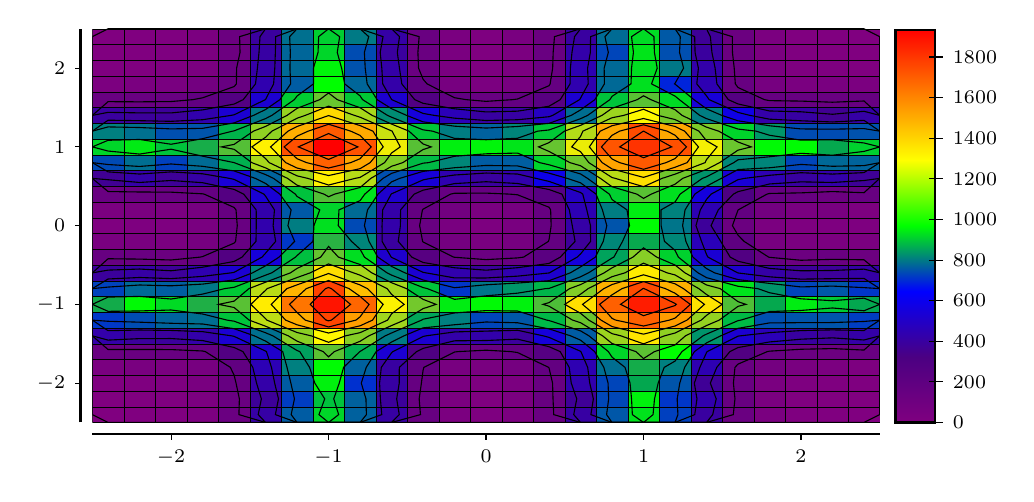
\begin{tikzpicture}
\begin{scope}[]
\pgfpathmoveto{ \pgfpointadd{\pgfpointxy {0.0} {0.0}} {\pgfpoint{0cm}{0cm}} }
\pgfpathlineto{ \pgfpointadd{\pgfpointxy {0.0} {0.0}} {\pgfpoint{10cm}{0cm}} }
\pgfpathlineto{ \pgfpointadd{\pgfpointxy {0.0} {0.0}} {\pgfpoint{10cm}{5cm}} }
\pgfpathlineto{ \pgfpointadd{\pgfpointxy {0.0} {0.0}} {\pgfpoint{0cm}{5cm}} }
\pgfpathclose
\pgfusepath{  clip, }
\begin{scope}[shift={(0.0,0.0)}]
\pgfsetxvec{\pgfpoint{2.0cm}{0cm}}
\pgfsetyvec{\pgfpoint{0cm}{1.0cm}}
\begin{scope}[shift={(2.5,2.5)}]
\begin{scope}[draw=black,ultra thin, fill=Indigo!0!violet]
\pgfpathmoveto{ \pgfpointxy {-2.5} {-2.5}}
\pgfpathlineto{ \pgfpointxy {-2.3} {-2.5}}
\pgfpathlineto{ \pgfpointxy {-2.3} {-2.3}}
\pgfpathlineto{ \pgfpointxy {-2.5} {-2.3}}
\pgfpathclose
\pgfusepath{ stroke, fill, }
\end{scope}
\begin{scope}[draw=black,ultra thin, fill=Indigo!0!violet]
\pgfpathmoveto{ \pgfpointxy {-2.3} {-2.5}}
\pgfpathlineto{ \pgfpointxy {-2.1} {-2.5}}
\pgfpathlineto{ \pgfpointxy {-2.1} {-2.3}}
\pgfpathlineto{ \pgfpointxy {-2.3} {-2.3}}
\pgfpathclose
\pgfusepath{ stroke, fill, }
\end{scope}
\begin{scope}[draw=black,ultra thin, fill=Indigo!1!violet]
\pgfpathmoveto{ \pgfpointxy {-2.1} {-2.5}}
\pgfpathlineto{ \pgfpointxy {-1.8999999} {-2.5}}
\pgfpathlineto{ \pgfpointxy {-1.8999999} {-2.3}}
\pgfpathlineto{ \pgfpointxy {-2.1} {-2.3}}
\pgfpathclose
\pgfusepath{ stroke, fill, }
\end{scope}
\begin{scope}[draw=black,ultra thin, fill=Indigo!6!violet]
\pgfpathmoveto{ \pgfpointxy {-1.9} {-2.5}}
\pgfpathlineto{ \pgfpointxy {-1.6999999} {-2.5}}
\pgfpathlineto{ \pgfpointxy {-1.6999999} {-2.3}}
\pgfpathlineto{ \pgfpointxy {-1.9} {-2.3}}
\pgfpathclose
\pgfusepath{ stroke, fill, }
\end{scope}
\begin{scope}[draw=black,ultra thin, fill=Indigo!40!violet]
\pgfpathmoveto{ \pgfpointxy {-1.7} {-2.5}}
\pgfpathlineto{ \pgfpointxy {-1.5} {-2.5}}
\pgfpathlineto{ \pgfpointxy {-1.5} {-2.3}}
\pgfpathlineto{ \pgfpointxy {-1.7} {-2.3}}
\pgfpathclose
\pgfusepath{ stroke, fill, }
\end{scope}
\begin{scope}[draw=black,ultra thin, fill=blue!28!Indigo]
\pgfpathmoveto{ \pgfpointxy {-1.5} {-2.5}}
\pgfpathlineto{ \pgfpointxy {-1.3} {-2.5}}
\pgfpathlineto{ \pgfpointxy {-1.3} {-2.3}}
\pgfpathlineto{ \pgfpointxy {-1.5} {-2.3}}
\pgfpathclose
\pgfusepath{ stroke, fill, }
\end{scope}
\begin{scope}[draw=black,ultra thin, fill=green!36!blue]
\pgfpathmoveto{ \pgfpointxy {-1.3} {-2.5}}
\pgfpathlineto{ \pgfpointxy {-1.0999999} {-2.5}}
\pgfpathlineto{ \pgfpointxy {-1.0999999} {-2.3}}
\pgfpathlineto{ \pgfpointxy {-1.3} {-2.3}}
\pgfpathclose
\pgfusepath{ stroke, fill, }
\end{scope}
\begin{scope}[draw=black,ultra thin, fill=green!84!blue]
\pgfpathmoveto{ \pgfpointxy {-1.1} {-2.5}}
\pgfpathlineto{ \pgfpointxy {-0.90000004} {-2.5}}
\pgfpathlineto{ \pgfpointxy {-0.90000004} {-2.3}}
\pgfpathlineto{ \pgfpointxy {-1.1} {-2.3}}
\pgfpathclose
\pgfusepath{ stroke, fill, }
\end{scope}
\begin{scope}[draw=black,ultra thin, fill=green!38!blue]
\pgfpathmoveto{ \pgfpointxy {-0.9} {-2.5}}
\pgfpathlineto{ \pgfpointxy {-0.7} {-2.5}}
\pgfpathlineto{ \pgfpointxy {-0.7} {-2.3}}
\pgfpathlineto{ \pgfpointxy {-0.9} {-2.3}}
\pgfpathclose
\pgfusepath{ stroke, fill, }
\end{scope}
\begin{scope}[draw=black,ultra thin, fill=blue!27!Indigo]
\pgfpathmoveto{ \pgfpointxy {-0.6999999} {-2.5}}
\pgfpathlineto{ \pgfpointxy {-0.49999994} {-2.5}}
\pgfpathlineto{ \pgfpointxy {-0.49999994} {-2.3}}
\pgfpathlineto{ \pgfpointxy {-0.6999999} {-2.3}}
\pgfpathclose
\pgfusepath{ stroke, fill, }
\end{scope}
\begin{scope}[draw=black,ultra thin, fill=Indigo!47!violet]
\pgfpathmoveto{ \pgfpointxy {-0.5} {-2.5}}
\pgfpathlineto{ \pgfpointxy {-0.3} {-2.5}}
\pgfpathlineto{ \pgfpointxy {-0.3} {-2.3}}
\pgfpathlineto{ \pgfpointxy {-0.5} {-2.3}}
\pgfpathclose
\pgfusepath{ stroke, fill, }
\end{scope}
\begin{scope}[draw=black,ultra thin, fill=Indigo!8!violet]
\pgfpathmoveto{ \pgfpointxy {-0.29999995} {-2.5}}
\pgfpathlineto{ \pgfpointxy {-0.09999995} {-2.5}}
\pgfpathlineto{ \pgfpointxy {-0.09999995} {-2.3}}
\pgfpathlineto{ \pgfpointxy {-0.29999995} {-2.3}}
\pgfpathclose
\pgfusepath{ stroke, fill, }
\end{scope}
\begin{scope}[draw=black,ultra thin, fill=Indigo!2!violet]
\pgfpathmoveto{ \pgfpointxy {-0.099999905} {-2.5}}
\pgfpathlineto{ \pgfpointxy {0.1000001} {-2.5}}
\pgfpathlineto{ \pgfpointxy {0.1000001} {-2.3}}
\pgfpathlineto{ \pgfpointxy {-0.099999905} {-2.3}}
\pgfpathclose
\pgfusepath{ stroke, fill, }
\end{scope}
\begin{scope}[draw=black,ultra thin, fill=Indigo!9!violet]
\pgfpathmoveto{ \pgfpointxy {0.10000014} {-2.5}}
\pgfpathlineto{ \pgfpointxy {0.30000013} {-2.5}}
\pgfpathlineto{ \pgfpointxy {0.30000013} {-2.3}}
\pgfpathlineto{ \pgfpointxy {0.10000014} {-2.3}}
\pgfpathclose
\pgfusepath{ stroke, fill, }
\end{scope}
\begin{scope}[draw=black,ultra thin, fill=Indigo!41!violet]
\pgfpathmoveto{ \pgfpointxy {0.29999995} {-2.5}}
\pgfpathlineto{ \pgfpointxy {0.49999994} {-2.5}}
\pgfpathlineto{ \pgfpointxy {0.49999994} {-2.3}}
\pgfpathlineto{ \pgfpointxy {0.29999995} {-2.3}}
\pgfpathclose
\pgfusepath{ stroke, fill, }
\end{scope}
\begin{scope}[draw=black,ultra thin, fill=blue!26!Indigo]
\pgfpathmoveto{ \pgfpointxy {0.5} {-2.5}}
\pgfpathlineto{ \pgfpointxy {0.7} {-2.5}}
\pgfpathlineto{ \pgfpointxy {0.7} {-2.3}}
\pgfpathlineto{ \pgfpointxy {0.5} {-2.3}}
\pgfpathclose
\pgfusepath{ stroke, fill, }
\end{scope}
\begin{scope}[draw=black,ultra thin, fill=green!34!blue]
\pgfpathmoveto{ \pgfpointxy {0.70000005} {-2.5}}
\pgfpathlineto{ \pgfpointxy {0.90000004} {-2.5}}
\pgfpathlineto{ \pgfpointxy {0.90000004} {-2.3}}
\pgfpathlineto{ \pgfpointxy {0.70000005} {-2.3}}
\pgfpathclose
\pgfusepath{ stroke, fill, }
\end{scope}
\begin{scope}[draw=black,ultra thin, fill=green!89!blue]
\pgfpathmoveto{ \pgfpointxy {0.9000001} {-2.5}}
\pgfpathlineto{ \pgfpointxy {1.1000001} {-2.5}}
\pgfpathlineto{ \pgfpointxy {1.1000001} {-2.3}}
\pgfpathlineto{ \pgfpointxy {0.9000001} {-2.3}}
\pgfpathclose
\pgfusepath{ stroke, fill, }
\end{scope}
\begin{scope}[draw=black,ultra thin, fill=green!25!blue]
\pgfpathmoveto{ \pgfpointxy {1.1000001} {-2.5}}
\pgfpathlineto{ \pgfpointxy {1.3000002} {-2.5}}
\pgfpathlineto{ \pgfpointxy {1.3000002} {-2.3}}
\pgfpathlineto{ \pgfpointxy {1.1000001} {-2.3}}
\pgfpathclose
\pgfusepath{ stroke, fill, }
\end{scope}
\begin{scope}[draw=black,ultra thin, fill=blue!24!Indigo]
\pgfpathmoveto{ \pgfpointxy {1.3} {-2.5}}
\pgfpathlineto{ \pgfpointxy {1.5} {-2.5}}
\pgfpathlineto{ \pgfpointxy {1.5} {-2.3}}
\pgfpathlineto{ \pgfpointxy {1.3} {-2.3}}
\pgfpathclose
\pgfusepath{ stroke, fill, }
\end{scope}
\begin{scope}[draw=black,ultra thin, fill=Indigo!41!violet]
\pgfpathmoveto{ \pgfpointxy {1.5} {-2.5}}
\pgfpathlineto{ \pgfpointxy {1.7} {-2.5}}
\pgfpathlineto{ \pgfpointxy {1.7} {-2.3}}
\pgfpathlineto{ \pgfpointxy {1.5} {-2.3}}
\pgfpathclose
\pgfusepath{ stroke, fill, }
\end{scope}
\begin{scope}[draw=black,ultra thin, fill=Indigo!10!violet]
\pgfpathmoveto{ \pgfpointxy {1.7000003} {-2.5}}
\pgfpathlineto{ \pgfpointxy {1.9000003} {-2.5}}
\pgfpathlineto{ \pgfpointxy {1.9000003} {-2.3}}
\pgfpathlineto{ \pgfpointxy {1.7000003} {-2.3}}
\pgfpathclose
\pgfusepath{ stroke, fill, }
\end{scope}
\begin{scope}[draw=black,ultra thin, fill=Indigo!1!violet]
\pgfpathmoveto{ \pgfpointxy {1.9000001} {-2.5}}
\pgfpathlineto{ \pgfpointxy {2.1000001} {-2.5}}
\pgfpathlineto{ \pgfpointxy {2.1000001} {-2.3}}
\pgfpathlineto{ \pgfpointxy {1.9000001} {-2.3}}
\pgfpathclose
\pgfusepath{ stroke, fill, }
\end{scope}
\begin{scope}[draw=black,ultra thin, fill=Indigo!0!violet]
\pgfpathmoveto{ \pgfpointxy {2.1} {-2.5}}
\pgfpathlineto{ \pgfpointxy {2.3} {-2.5}}
\pgfpathlineto{ \pgfpointxy {2.3} {-2.3}}
\pgfpathlineto{ \pgfpointxy {2.1} {-2.3}}
\pgfpathclose
\pgfusepath{ stroke, fill, }
\end{scope}
\begin{scope}[draw=black,ultra thin, fill=Indigo!0!violet]
\pgfpathmoveto{ \pgfpointxy {2.3000002} {-2.5}}
\pgfpathlineto{ \pgfpointxy {2.5000002} {-2.5}}
\pgfpathlineto{ \pgfpointxy {2.5000002} {-2.3}}
\pgfpathlineto{ \pgfpointxy {2.3000002} {-2.3}}
\pgfpathclose
\pgfusepath{ stroke, fill, }
\end{scope}
\begin{scope}[draw=black,ultra thin, fill=Indigo!0!violet]
\pgfpathmoveto{ \pgfpointxy {-2.5} {-2.3}}
\pgfpathlineto{ \pgfpointxy {-2.3} {-2.3}}
\pgfpathlineto{ \pgfpointxy {-2.3} {-2.1}}
\pgfpathlineto{ \pgfpointxy {-2.5} {-2.1}}
\pgfpathclose
\pgfusepath{ stroke, fill, }
\end{scope}
\begin{scope}[draw=black,ultra thin, fill=Indigo!0!violet]
\pgfpathmoveto{ \pgfpointxy {-2.3} {-2.3}}
\pgfpathlineto{ \pgfpointxy {-2.1} {-2.3}}
\pgfpathlineto{ \pgfpointxy {-2.1} {-2.1}}
\pgfpathlineto{ \pgfpointxy {-2.3} {-2.1}}
\pgfpathclose
\pgfusepath{ stroke, fill, }
\end{scope}
\begin{scope}[draw=black,ultra thin, fill=Indigo!1!violet]
\pgfpathmoveto{ \pgfpointxy {-2.1} {-2.3}}
\pgfpathlineto{ \pgfpointxy {-1.8999999} {-2.3}}
\pgfpathlineto{ \pgfpointxy {-1.8999999} {-2.1}}
\pgfpathlineto{ \pgfpointxy {-2.1} {-2.1}}
\pgfpathclose
\pgfusepath{ stroke, fill, }
\end{scope}
\begin{scope}[draw=black,ultra thin, fill=Indigo!8!violet]
\pgfpathmoveto{ \pgfpointxy {-1.9} {-2.3}}
\pgfpathlineto{ \pgfpointxy {-1.6999999} {-2.3}}
\pgfpathlineto{ \pgfpointxy {-1.6999999} {-2.1}}
\pgfpathlineto{ \pgfpointxy {-1.9} {-2.1}}
\pgfpathclose
\pgfusepath{ stroke, fill, }
\end{scope}
\begin{scope}[draw=black,ultra thin, fill=Indigo!41!violet]
\pgfpathmoveto{ \pgfpointxy {-1.7} {-2.3}}
\pgfpathlineto{ \pgfpointxy {-1.5} {-2.3}}
\pgfpathlineto{ \pgfpointxy {-1.5} {-2.1}}
\pgfpathlineto{ \pgfpointxy {-1.7} {-2.1}}
\pgfpathclose
\pgfusepath{ stroke, fill, }
\end{scope}
\begin{scope}[draw=black,ultra thin, fill=blue!18!Indigo]
\pgfpathmoveto{ \pgfpointxy {-1.5} {-2.3}}
\pgfpathlineto{ \pgfpointxy {-1.3} {-2.3}}
\pgfpathlineto{ \pgfpointxy {-1.3} {-2.1}}
\pgfpathlineto{ \pgfpointxy {-1.5} {-2.1}}
\pgfpathclose
\pgfusepath{ stroke, fill, }
\end{scope}
\begin{scope}[draw=black,ultra thin, fill=green!24!blue]
\pgfpathmoveto{ \pgfpointxy {-1.3} {-2.3}}
\pgfpathlineto{ \pgfpointxy {-1.0999999} {-2.3}}
\pgfpathlineto{ \pgfpointxy {-1.0999999} {-2.1}}
\pgfpathlineto{ \pgfpointxy {-1.3} {-2.1}}
\pgfpathclose
\pgfusepath{ stroke, fill, }
\end{scope}
\begin{scope}[draw=black,ultra thin, fill=green!76!blue]
\pgfpathmoveto{ \pgfpointxy {-1.1} {-2.3}}
\pgfpathlineto{ \pgfpointxy {-0.90000004} {-2.3}}
\pgfpathlineto{ \pgfpointxy {-0.90000004} {-2.1}}
\pgfpathlineto{ \pgfpointxy {-1.1} {-2.1}}
\pgfpathclose
\pgfusepath{ stroke, fill, }
\end{scope}
\begin{scope}[draw=black,ultra thin, fill=green!38!blue]
\pgfpathmoveto{ \pgfpointxy {-0.9} {-2.3}}
\pgfpathlineto{ \pgfpointxy {-0.7} {-2.3}}
\pgfpathlineto{ \pgfpointxy {-0.7} {-2.1}}
\pgfpathlineto{ \pgfpointxy {-0.9} {-2.1}}
\pgfpathclose
\pgfusepath{ stroke, fill, }
\end{scope}
\begin{scope}[draw=black,ultra thin, fill=blue!20!Indigo]
\pgfpathmoveto{ \pgfpointxy {-0.6999999} {-2.3}}
\pgfpathlineto{ \pgfpointxy {-0.49999994} {-2.3}}
\pgfpathlineto{ \pgfpointxy {-0.49999994} {-2.1}}
\pgfpathlineto{ \pgfpointxy {-0.6999999} {-2.1}}
\pgfpathclose
\pgfusepath{ stroke, fill, }
\end{scope}
\begin{scope}[draw=black,ultra thin, fill=Indigo!44!violet]
\pgfpathmoveto{ \pgfpointxy {-0.5} {-2.3}}
\pgfpathlineto{ \pgfpointxy {-0.3} {-2.3}}
\pgfpathlineto{ \pgfpointxy {-0.3} {-2.1}}
\pgfpathlineto{ \pgfpointxy {-0.5} {-2.1}}
\pgfpathclose
\pgfusepath{ stroke, fill, }
\end{scope}
\begin{scope}[draw=black,ultra thin, fill=Indigo!10!violet]
\pgfpathmoveto{ \pgfpointxy {-0.29999995} {-2.3}}
\pgfpathlineto{ \pgfpointxy {-0.09999995} {-2.3}}
\pgfpathlineto{ \pgfpointxy {-0.09999995} {-2.1}}
\pgfpathlineto{ \pgfpointxy {-0.29999995} {-2.1}}
\pgfpathclose
\pgfusepath{ stroke, fill, }
\end{scope}
\begin{scope}[draw=black,ultra thin, fill=Indigo!1!violet]
\pgfpathmoveto{ \pgfpointxy {-0.099999905} {-2.3}}
\pgfpathlineto{ \pgfpointxy {0.1000001} {-2.3}}
\pgfpathlineto{ \pgfpointxy {0.1000001} {-2.1}}
\pgfpathlineto{ \pgfpointxy {-0.099999905} {-2.1}}
\pgfpathclose
\pgfusepath{ stroke, fill, }
\end{scope}
\begin{scope}[draw=black,ultra thin, fill=Indigo!10!violet]
\pgfpathmoveto{ \pgfpointxy {0.10000014} {-2.3}}
\pgfpathlineto{ \pgfpointxy {0.30000013} {-2.3}}
\pgfpathlineto{ \pgfpointxy {0.30000013} {-2.1}}
\pgfpathlineto{ \pgfpointxy {0.10000014} {-2.1}}
\pgfpathclose
\pgfusepath{ stroke, fill, }
\end{scope}
\begin{scope}[draw=black,ultra thin, fill=Indigo!44!violet]
\pgfpathmoveto{ \pgfpointxy {0.29999995} {-2.3}}
\pgfpathlineto{ \pgfpointxy {0.49999994} {-2.3}}
\pgfpathlineto{ \pgfpointxy {0.49999994} {-2.1}}
\pgfpathlineto{ \pgfpointxy {0.29999995} {-2.1}}
\pgfpathclose
\pgfusepath{ stroke, fill, }
\end{scope}
\begin{scope}[draw=black,ultra thin, fill=blue!16!Indigo]
\pgfpathmoveto{ \pgfpointxy {0.5} {-2.3}}
\pgfpathlineto{ \pgfpointxy {0.7} {-2.3}}
\pgfpathlineto{ \pgfpointxy {0.7} {-2.1}}
\pgfpathlineto{ \pgfpointxy {0.5} {-2.1}}
\pgfpathclose
\pgfusepath{ stroke, fill, }
\end{scope}
\begin{scope}[draw=black,ultra thin, fill=green!28!blue]
\pgfpathmoveto{ \pgfpointxy {0.70000005} {-2.3}}
\pgfpathlineto{ \pgfpointxy {0.90000004} {-2.3}}
\pgfpathlineto{ \pgfpointxy {0.90000004} {-2.1}}
\pgfpathlineto{ \pgfpointxy {0.70000005} {-2.1}}
\pgfpathclose
\pgfusepath{ stroke, fill, }
\end{scope}
\begin{scope}[draw=black,ultra thin, fill=green!95!blue]
\pgfpathmoveto{ \pgfpointxy {0.9000001} {-2.3}}
\pgfpathlineto{ \pgfpointxy {1.1000001} {-2.3}}
\pgfpathlineto{ \pgfpointxy {1.1000001} {-2.1}}
\pgfpathlineto{ \pgfpointxy {0.9000001} {-2.1}}
\pgfpathclose
\pgfusepath{ stroke, fill, }
\end{scope}
\begin{scope}[draw=black,ultra thin, fill=green!21!blue]
\pgfpathmoveto{ \pgfpointxy {1.1000001} {-2.3}}
\pgfpathlineto{ \pgfpointxy {1.3000002} {-2.3}}
\pgfpathlineto{ \pgfpointxy {1.3000002} {-2.1}}
\pgfpathlineto{ \pgfpointxy {1.1000001} {-2.1}}
\pgfpathclose
\pgfusepath{ stroke, fill, }
\end{scope}
\begin{scope}[draw=black,ultra thin, fill=blue!35!Indigo]
\pgfpathmoveto{ \pgfpointxy {1.3} {-2.3}}
\pgfpathlineto{ \pgfpointxy {1.5} {-2.3}}
\pgfpathlineto{ \pgfpointxy {1.5} {-2.1}}
\pgfpathlineto{ \pgfpointxy {1.3} {-2.1}}
\pgfpathclose
\pgfusepath{ stroke, fill, }
\end{scope}
\begin{scope}[draw=black,ultra thin, fill=Indigo!45!violet]
\pgfpathmoveto{ \pgfpointxy {1.5} {-2.3}}
\pgfpathlineto{ \pgfpointxy {1.7} {-2.3}}
\pgfpathlineto{ \pgfpointxy {1.7} {-2.1}}
\pgfpathlineto{ \pgfpointxy {1.5} {-2.1}}
\pgfpathclose
\pgfusepath{ stroke, fill, }
\end{scope}
\begin{scope}[draw=black,ultra thin, fill=Indigo!11!violet]
\pgfpathmoveto{ \pgfpointxy {1.7000003} {-2.3}}
\pgfpathlineto{ \pgfpointxy {1.9000003} {-2.3}}
\pgfpathlineto{ \pgfpointxy {1.9000003} {-2.1}}
\pgfpathlineto{ \pgfpointxy {1.7000003} {-2.1}}
\pgfpathclose
\pgfusepath{ stroke, fill, }
\end{scope}
\begin{scope}[draw=black,ultra thin, fill=Indigo!0!violet]
\pgfpathmoveto{ \pgfpointxy {1.9000001} {-2.3}}
\pgfpathlineto{ \pgfpointxy {2.1000001} {-2.3}}
\pgfpathlineto{ \pgfpointxy {2.1000001} {-2.1}}
\pgfpathlineto{ \pgfpointxy {1.9000001} {-2.1}}
\pgfpathclose
\pgfusepath{ stroke, fill, }
\end{scope}
\begin{scope}[draw=black,ultra thin, fill=Indigo!0!violet]
\pgfpathmoveto{ \pgfpointxy {2.1} {-2.3}}
\pgfpathlineto{ \pgfpointxy {2.3} {-2.3}}
\pgfpathlineto{ \pgfpointxy {2.3} {-2.1}}
\pgfpathlineto{ \pgfpointxy {2.1} {-2.1}}
\pgfpathclose
\pgfusepath{ stroke, fill, }
\end{scope}
\begin{scope}[draw=black,ultra thin, fill=Indigo!0!violet]
\pgfpathmoveto{ \pgfpointxy {2.3000002} {-2.3}}
\pgfpathlineto{ \pgfpointxy {2.5000002} {-2.3}}
\pgfpathlineto{ \pgfpointxy {2.5000002} {-2.1}}
\pgfpathlineto{ \pgfpointxy {2.3000002} {-2.1}}
\pgfpathclose
\pgfusepath{ stroke, fill, }
\end{scope}
\begin{scope}[draw=black,ultra thin, fill=Indigo!1!violet]
\pgfpathmoveto{ \pgfpointxy {-2.5} {-2.1}}
\pgfpathlineto{ \pgfpointxy {-2.3} {-2.1}}
\pgfpathlineto{ \pgfpointxy {-2.3} {-1.8999999}}
\pgfpathlineto{ \pgfpointxy {-2.5} {-1.8999999}}
\pgfpathclose
\pgfusepath{ stroke, fill, }
\end{scope}
\begin{scope}[draw=black,ultra thin, fill=Indigo!1!violet]
\pgfpathmoveto{ \pgfpointxy {-2.3} {-2.1}}
\pgfpathlineto{ \pgfpointxy {-2.1} {-2.1}}
\pgfpathlineto{ \pgfpointxy {-2.1} {-1.8999999}}
\pgfpathlineto{ \pgfpointxy {-2.3} {-1.8999999}}
\pgfpathclose
\pgfusepath{ stroke, fill, }
\end{scope}
\begin{scope}[draw=black,ultra thin, fill=Indigo!2!violet]
\pgfpathmoveto{ \pgfpointxy {-2.1} {-2.1}}
\pgfpathlineto{ \pgfpointxy {-1.8999999} {-2.1}}
\pgfpathlineto{ \pgfpointxy {-1.8999999} {-1.8999999}}
\pgfpathlineto{ \pgfpointxy {-2.1} {-1.8999999}}
\pgfpathclose
\pgfusepath{ stroke, fill, }
\end{scope}
\begin{scope}[draw=black,ultra thin, fill=Indigo!12!violet]
\pgfpathmoveto{ \pgfpointxy {-1.9} {-2.1}}
\pgfpathlineto{ \pgfpointxy {-1.6999999} {-2.1}}
\pgfpathlineto{ \pgfpointxy {-1.6999999} {-1.8999999}}
\pgfpathlineto{ \pgfpointxy {-1.9} {-1.8999999}}
\pgfpathclose
\pgfusepath{ stroke, fill, }
\end{scope}
\begin{scope}[draw=black,ultra thin, fill=Indigo!48!violet]
\pgfpathmoveto{ \pgfpointxy {-1.7} {-2.1}}
\pgfpathlineto{ \pgfpointxy {-1.5} {-2.1}}
\pgfpathlineto{ \pgfpointxy {-1.5} {-1.8999999}}
\pgfpathlineto{ \pgfpointxy {-1.7} {-1.8999999}}
\pgfpathclose
\pgfusepath{ stroke, fill, }
\end{scope}
\begin{scope}[draw=black,ultra thin, fill=blue!31!Indigo]
\pgfpathmoveto{ \pgfpointxy {-1.5} {-2.1}}
\pgfpathlineto{ \pgfpointxy {-1.3} {-2.1}}
\pgfpathlineto{ \pgfpointxy {-1.3} {-1.8999999}}
\pgfpathlineto{ \pgfpointxy {-1.5} {-1.8999999}}
\pgfpathclose
\pgfusepath{ stroke, fill, }
\end{scope}
\begin{scope}[draw=black,ultra thin, fill=green!36!blue]
\pgfpathmoveto{ \pgfpointxy {-1.3} {-2.1}}
\pgfpathlineto{ \pgfpointxy {-1.0999999} {-2.1}}
\pgfpathlineto{ \pgfpointxy {-1.0999999} {-1.8999999}}
\pgfpathlineto{ \pgfpointxy {-1.3} {-1.8999999}}
\pgfpathclose
\pgfusepath{ stroke, fill, }
\end{scope}
\begin{scope}[draw=black,ultra thin, fill=green!95!blue]
\pgfpathmoveto{ \pgfpointxy {-1.1} {-2.1}}
\pgfpathlineto{ \pgfpointxy {-0.90000004} {-2.1}}
\pgfpathlineto{ \pgfpointxy {-0.90000004} {-1.8999999}}
\pgfpathlineto{ \pgfpointxy {-1.1} {-1.8999999}}
\pgfpathclose
\pgfusepath{ stroke, fill, }
\end{scope}
\begin{scope}[draw=black,ultra thin, fill=green!19!blue]
\pgfpathmoveto{ \pgfpointxy {-0.9} {-2.1}}
\pgfpathlineto{ \pgfpointxy {-0.7} {-2.1}}
\pgfpathlineto{ \pgfpointxy {-0.7} {-1.8999999}}
\pgfpathlineto{ \pgfpointxy {-0.9} {-1.8999999}}
\pgfpathclose
\pgfusepath{ stroke, fill, }
\end{scope}
\begin{scope}[draw=black,ultra thin, fill=blue!26!Indigo]
\pgfpathmoveto{ \pgfpointxy {-0.6999999} {-2.1}}
\pgfpathlineto{ \pgfpointxy {-0.49999994} {-2.1}}
\pgfpathlineto{ \pgfpointxy {-0.49999994} {-1.8999999}}
\pgfpathlineto{ \pgfpointxy {-0.6999999} {-1.8999999}}
\pgfpathclose
\pgfusepath{ stroke, fill, }
\end{scope}
\begin{scope}[draw=black,ultra thin, fill=Indigo!49!violet]
\pgfpathmoveto{ \pgfpointxy {-0.5} {-2.1}}
\pgfpathlineto{ \pgfpointxy {-0.3} {-2.1}}
\pgfpathlineto{ \pgfpointxy {-0.3} {-1.8999999}}
\pgfpathlineto{ \pgfpointxy {-0.5} {-1.8999999}}
\pgfpathclose
\pgfusepath{ stroke, fill, }
\end{scope}
\begin{scope}[draw=black,ultra thin, fill=Indigo!9!violet]
\pgfpathmoveto{ \pgfpointxy {-0.29999995} {-2.1}}
\pgfpathlineto{ \pgfpointxy {-0.09999995} {-2.1}}
\pgfpathlineto{ \pgfpointxy {-0.09999995} {-1.8999999}}
\pgfpathlineto{ \pgfpointxy {-0.29999995} {-1.8999999}}
\pgfpathclose
\pgfusepath{ stroke, fill, }
\end{scope}
\begin{scope}[draw=black,ultra thin, fill=Indigo!5!violet]
\pgfpathmoveto{ \pgfpointxy {-0.099999905} {-2.1}}
\pgfpathlineto{ \pgfpointxy {0.1000001} {-2.1}}
\pgfpathlineto{ \pgfpointxy {0.1000001} {-1.8999999}}
\pgfpathlineto{ \pgfpointxy {-0.099999905} {-1.8999999}}
\pgfpathclose
\pgfusepath{ stroke, fill, }
\end{scope}
\begin{scope}[draw=black,ultra thin, fill=Indigo!9!violet]
\pgfpathmoveto{ \pgfpointxy {0.10000014} {-2.1}}
\pgfpathlineto{ \pgfpointxy {0.30000013} {-2.1}}
\pgfpathlineto{ \pgfpointxy {0.30000013} {-1.8999999}}
\pgfpathlineto{ \pgfpointxy {0.10000014} {-1.8999999}}
\pgfpathclose
\pgfusepath{ stroke, fill, }
\end{scope}
\begin{scope}[draw=black,ultra thin, fill=Indigo!43!violet]
\pgfpathmoveto{ \pgfpointxy {0.29999995} {-2.1}}
\pgfpathlineto{ \pgfpointxy {0.49999994} {-2.1}}
\pgfpathlineto{ \pgfpointxy {0.49999994} {-1.8999999}}
\pgfpathlineto{ \pgfpointxy {0.29999995} {-1.8999999}}
\pgfpathclose
\pgfusepath{ stroke, fill, }
\end{scope}
\begin{scope}[draw=black,ultra thin, fill=blue!34!Indigo]
\pgfpathmoveto{ \pgfpointxy {0.5} {-2.1}}
\pgfpathlineto{ \pgfpointxy {0.7} {-2.1}}
\pgfpathlineto{ \pgfpointxy {0.7} {-1.8999999}}
\pgfpathlineto{ \pgfpointxy {0.5} {-1.8999999}}
\pgfpathclose
\pgfusepath{ stroke, fill, }
\end{scope}
\begin{scope}[draw=black,ultra thin, fill=green!27!blue]
\pgfpathmoveto{ \pgfpointxy {0.70000005} {-2.1}}
\pgfpathlineto{ \pgfpointxy {0.90000004} {-2.1}}
\pgfpathlineto{ \pgfpointxy {0.90000004} {-1.8999999}}
\pgfpathlineto{ \pgfpointxy {0.70000005} {-1.8999999}}
\pgfpathclose
\pgfusepath{ stroke, fill, }
\end{scope}
\begin{scope}[draw=black,ultra thin, fill=yellow!1!green]
\pgfpathmoveto{ \pgfpointxy {0.9000001} {-2.1}}
\pgfpathlineto{ \pgfpointxy {1.1000001} {-2.1}}
\pgfpathlineto{ \pgfpointxy {1.1000001} {-1.8999999}}
\pgfpathlineto{ \pgfpointxy {0.9000001} {-1.8999999}}
\pgfpathclose
\pgfusepath{ stroke, fill, }
\end{scope}
\begin{scope}[draw=black,ultra thin, fill=green!33!blue]
\pgfpathmoveto{ \pgfpointxy {1.1000001} {-2.1}}
\pgfpathlineto{ \pgfpointxy {1.3000002} {-2.1}}
\pgfpathlineto{ \pgfpointxy {1.3000002} {-1.8999999}}
\pgfpathlineto{ \pgfpointxy {1.1000001} {-1.8999999}}
\pgfpathclose
\pgfusepath{ stroke, fill, }
\end{scope}
\begin{scope}[draw=black,ultra thin, fill=blue!16!Indigo]
\pgfpathmoveto{ \pgfpointxy {1.3} {-2.1}}
\pgfpathlineto{ \pgfpointxy {1.5} {-2.1}}
\pgfpathlineto{ \pgfpointxy {1.5} {-1.8999999}}
\pgfpathlineto{ \pgfpointxy {1.3} {-1.8999999}}
\pgfpathclose
\pgfusepath{ stroke, fill, }
\end{scope}
\begin{scope}[draw=black,ultra thin, fill=Indigo!43!violet]
\pgfpathmoveto{ \pgfpointxy {1.5} {-2.1}}
\pgfpathlineto{ \pgfpointxy {1.7} {-2.1}}
\pgfpathlineto{ \pgfpointxy {1.7} {-1.8999999}}
\pgfpathlineto{ \pgfpointxy {1.5} {-1.8999999}}
\pgfpathclose
\pgfusepath{ stroke, fill, }
\end{scope}
\begin{scope}[draw=black,ultra thin, fill=Indigo!11!violet]
\pgfpathmoveto{ \pgfpointxy {1.7000003} {-2.1}}
\pgfpathlineto{ \pgfpointxy {1.9000003} {-2.1}}
\pgfpathlineto{ \pgfpointxy {1.9000003} {-1.8999999}}
\pgfpathlineto{ \pgfpointxy {1.7000003} {-1.8999999}}
\pgfpathclose
\pgfusepath{ stroke, fill, }
\end{scope}
\begin{scope}[draw=black,ultra thin, fill=Indigo!2!violet]
\pgfpathmoveto{ \pgfpointxy {1.9000001} {-2.1}}
\pgfpathlineto{ \pgfpointxy {2.1000001} {-2.1}}
\pgfpathlineto{ \pgfpointxy {2.1000001} {-1.8999999}}
\pgfpathlineto{ \pgfpointxy {1.9000001} {-1.8999999}}
\pgfpathclose
\pgfusepath{ stroke, fill, }
\end{scope}
\begin{scope}[draw=black,ultra thin, fill=Indigo!1!violet]
\pgfpathmoveto{ \pgfpointxy {2.1} {-2.1}}
\pgfpathlineto{ \pgfpointxy {2.3} {-2.1}}
\pgfpathlineto{ \pgfpointxy {2.3} {-1.8999999}}
\pgfpathlineto{ \pgfpointxy {2.1} {-1.8999999}}
\pgfpathclose
\pgfusepath{ stroke, fill, }
\end{scope}
\begin{scope}[draw=black,ultra thin, fill=Indigo!1!violet]
\pgfpathmoveto{ \pgfpointxy {2.3000002} {-2.1}}
\pgfpathlineto{ \pgfpointxy {2.5000002} {-2.1}}
\pgfpathlineto{ \pgfpointxy {2.5000002} {-1.8999999}}
\pgfpathlineto{ \pgfpointxy {2.3000002} {-1.8999999}}
\pgfpathclose
\pgfusepath{ stroke, fill, }
\end{scope}
\begin{scope}[draw=black,ultra thin, fill=Indigo!10!violet]
\pgfpathmoveto{ \pgfpointxy {-2.5} {-1.9}}
\pgfpathlineto{ \pgfpointxy {-2.3} {-1.9}}
\pgfpathlineto{ \pgfpointxy {-2.3} {-1.6999999}}
\pgfpathlineto{ \pgfpointxy {-2.5} {-1.6999999}}
\pgfpathclose
\pgfusepath{ stroke, fill, }
\end{scope}
\begin{scope}[draw=black,ultra thin, fill=Indigo!12!violet]
\pgfpathmoveto{ \pgfpointxy {-2.3} {-1.9}}
\pgfpathlineto{ \pgfpointxy {-2.1} {-1.9}}
\pgfpathlineto{ \pgfpointxy {-2.1} {-1.6999999}}
\pgfpathlineto{ \pgfpointxy {-2.3} {-1.6999999}}
\pgfpathclose
\pgfusepath{ stroke, fill, }
\end{scope}
\begin{scope}[draw=black,ultra thin, fill=Indigo!10!violet]
\pgfpathmoveto{ \pgfpointxy {-2.1} {-1.9}}
\pgfpathlineto{ \pgfpointxy {-1.8999999} {-1.9}}
\pgfpathlineto{ \pgfpointxy {-1.8999999} {-1.6999999}}
\pgfpathlineto{ \pgfpointxy {-2.1} {-1.6999999}}
\pgfpathclose
\pgfusepath{ stroke, fill, }
\end{scope}
\begin{scope}[draw=black,ultra thin, fill=Indigo!17!violet]
\pgfpathmoveto{ \pgfpointxy {-1.9} {-1.9}}
\pgfpathlineto{ \pgfpointxy {-1.6999999} {-1.9}}
\pgfpathlineto{ \pgfpointxy {-1.6999999} {-1.6999999}}
\pgfpathlineto{ \pgfpointxy {-1.9} {-1.6999999}}
\pgfpathclose
\pgfusepath{ stroke, fill, }
\end{scope}
\begin{scope}[draw=black,ultra thin, fill=Indigo!58!violet]
\pgfpathmoveto{ \pgfpointxy {-1.7} {-1.9}}
\pgfpathlineto{ \pgfpointxy {-1.5} {-1.9}}
\pgfpathlineto{ \pgfpointxy {-1.5} {-1.6999999}}
\pgfpathlineto{ \pgfpointxy {-1.7} {-1.6999999}}
\pgfpathclose
\pgfusepath{ stroke, fill, }
\end{scope}
\begin{scope}[draw=black,ultra thin, fill=blue!41!Indigo]
\pgfpathmoveto{ \pgfpointxy {-1.5} {-1.9}}
\pgfpathlineto{ \pgfpointxy {-1.3} {-1.9}}
\pgfpathlineto{ \pgfpointxy {-1.3} {-1.6999999}}
\pgfpathlineto{ \pgfpointxy {-1.5} {-1.6999999}}
\pgfpathclose
\pgfusepath{ stroke, fill, }
\end{scope}
\begin{scope}[draw=black,ultra thin, fill=green!50!blue]
\pgfpathmoveto{ \pgfpointxy {-1.3} {-1.9}}
\pgfpathlineto{ \pgfpointxy {-1.0999999} {-1.9}}
\pgfpathlineto{ \pgfpointxy {-1.0999999} {-1.6999999}}
\pgfpathlineto{ \pgfpointxy {-1.3} {-1.6999999}}
\pgfpathclose
\pgfusepath{ stroke, fill, }
\end{scope}
\begin{scope}[draw=black,ultra thin, fill=green!99!blue]
\pgfpathmoveto{ \pgfpointxy {-1.1} {-1.9}}
\pgfpathlineto{ \pgfpointxy {-0.90000004} {-1.9}}
\pgfpathlineto{ \pgfpointxy {-0.90000004} {-1.6999999}}
\pgfpathlineto{ \pgfpointxy {-1.1} {-1.6999999}}
\pgfpathclose
\pgfusepath{ stroke, fill, }
\end{scope}
\begin{scope}[draw=black,ultra thin, fill=green!38!blue]
\pgfpathmoveto{ \pgfpointxy {-0.9} {-1.9}}
\pgfpathlineto{ \pgfpointxy {-0.7} {-1.9}}
\pgfpathlineto{ \pgfpointxy {-0.7} {-1.6999999}}
\pgfpathlineto{ \pgfpointxy {-0.9} {-1.6999999}}
\pgfpathclose
\pgfusepath{ stroke, fill, }
\end{scope}
\begin{scope}[draw=black,ultra thin, fill=blue!25!Indigo]
\pgfpathmoveto{ \pgfpointxy {-0.6999999} {-1.9}}
\pgfpathlineto{ \pgfpointxy {-0.49999994} {-1.9}}
\pgfpathlineto{ \pgfpointxy {-0.49999994} {-1.6999999}}
\pgfpathlineto{ \pgfpointxy {-0.6999999} {-1.6999999}}
\pgfpathclose
\pgfusepath{ stroke, fill, }
\end{scope}
\begin{scope}[draw=black,ultra thin, fill=Indigo!54!violet]
\pgfpathmoveto{ \pgfpointxy {-0.5} {-1.9}}
\pgfpathlineto{ \pgfpointxy {-0.3} {-1.9}}
\pgfpathlineto{ \pgfpointxy {-0.3} {-1.6999999}}
\pgfpathlineto{ \pgfpointxy {-0.5} {-1.6999999}}
\pgfpathclose
\pgfusepath{ stroke, fill, }
\end{scope}
\begin{scope}[draw=black,ultra thin, fill=Indigo!15!violet]
\pgfpathmoveto{ \pgfpointxy {-0.29999995} {-1.9}}
\pgfpathlineto{ \pgfpointxy {-0.09999995} {-1.9}}
\pgfpathlineto{ \pgfpointxy {-0.09999995} {-1.6999999}}
\pgfpathlineto{ \pgfpointxy {-0.29999995} {-1.6999999}}
\pgfpathclose
\pgfusepath{ stroke, fill, }
\end{scope}
\begin{scope}[draw=black,ultra thin, fill=Indigo!12!violet]
\pgfpathmoveto{ \pgfpointxy {-0.099999905} {-1.9}}
\pgfpathlineto{ \pgfpointxy {0.1000001} {-1.9}}
\pgfpathlineto{ \pgfpointxy {0.1000001} {-1.6999999}}
\pgfpathlineto{ \pgfpointxy {-0.099999905} {-1.6999999}}
\pgfpathclose
\pgfusepath{ stroke, fill, }
\end{scope}
\begin{scope}[draw=black,ultra thin, fill=Indigo!20!violet]
\pgfpathmoveto{ \pgfpointxy {0.10000014} {-1.9}}
\pgfpathlineto{ \pgfpointxy {0.30000013} {-1.9}}
\pgfpathlineto{ \pgfpointxy {0.30000013} {-1.6999999}}
\pgfpathlineto{ \pgfpointxy {0.10000014} {-1.6999999}}
\pgfpathclose
\pgfusepath{ stroke, fill, }
\end{scope}
\begin{scope}[draw=black,ultra thin, fill=Indigo!54!violet]
\pgfpathmoveto{ \pgfpointxy {0.29999995} {-1.9}}
\pgfpathlineto{ \pgfpointxy {0.49999994} {-1.9}}
\pgfpathlineto{ \pgfpointxy {0.49999994} {-1.6999999}}
\pgfpathlineto{ \pgfpointxy {0.29999995} {-1.6999999}}
\pgfpathclose
\pgfusepath{ stroke, fill, }
\end{scope}
\begin{scope}[draw=black,ultra thin, fill=blue!38!Indigo]
\pgfpathmoveto{ \pgfpointxy {0.5} {-1.9}}
\pgfpathlineto{ \pgfpointxy {0.7} {-1.9}}
\pgfpathlineto{ \pgfpointxy {0.7} {-1.6999999}}
\pgfpathlineto{ \pgfpointxy {0.5} {-1.6999999}}
\pgfpathclose
\pgfusepath{ stroke, fill, }
\end{scope}
\begin{scope}[draw=black,ultra thin, fill=green!43!blue]
\pgfpathmoveto{ \pgfpointxy {0.70000005} {-1.9}}
\pgfpathlineto{ \pgfpointxy {0.90000004} {-1.9}}
\pgfpathlineto{ \pgfpointxy {0.90000004} {-1.6999999}}
\pgfpathlineto{ \pgfpointxy {0.70000005} {-1.6999999}}
\pgfpathclose
\pgfusepath{ stroke, fill, }
\end{scope}
\begin{scope}[draw=black,ultra thin, fill=yellow!8!green]
\pgfpathmoveto{ \pgfpointxy {0.9000001} {-1.9}}
\pgfpathlineto{ \pgfpointxy {1.1000001} {-1.9}}
\pgfpathlineto{ \pgfpointxy {1.1000001} {-1.6999999}}
\pgfpathlineto{ \pgfpointxy {0.9000001} {-1.6999999}}
\pgfpathclose
\pgfusepath{ stroke, fill, }
\end{scope}
\begin{scope}[draw=black,ultra thin, fill=green!50!blue]
\pgfpathmoveto{ \pgfpointxy {1.1000001} {-1.9}}
\pgfpathlineto{ \pgfpointxy {1.3000002} {-1.9}}
\pgfpathlineto{ \pgfpointxy {1.3000002} {-1.6999999}}
\pgfpathlineto{ \pgfpointxy {1.1000001} {-1.6999999}}
\pgfpathclose
\pgfusepath{ stroke, fill, }
\end{scope}
\begin{scope}[draw=black,ultra thin, fill=blue!38!Indigo]
\pgfpathmoveto{ \pgfpointxy {1.3} {-1.9}}
\pgfpathlineto{ \pgfpointxy {1.5} {-1.9}}
\pgfpathlineto{ \pgfpointxy {1.5} {-1.6999999}}
\pgfpathlineto{ \pgfpointxy {1.3} {-1.6999999}}
\pgfpathclose
\pgfusepath{ stroke, fill, }
\end{scope}
\begin{scope}[draw=black,ultra thin, fill=Indigo!44!violet]
\pgfpathmoveto{ \pgfpointxy {1.5} {-1.9}}
\pgfpathlineto{ \pgfpointxy {1.7} {-1.9}}
\pgfpathlineto{ \pgfpointxy {1.7} {-1.6999999}}
\pgfpathlineto{ \pgfpointxy {1.5} {-1.6999999}}
\pgfpathclose
\pgfusepath{ stroke, fill, }
\end{scope}
\begin{scope}[draw=black,ultra thin, fill=Indigo!21!violet]
\pgfpathmoveto{ \pgfpointxy {1.7000003} {-1.9}}
\pgfpathlineto{ \pgfpointxy {1.9000003} {-1.9}}
\pgfpathlineto{ \pgfpointxy {1.9000003} {-1.6999999}}
\pgfpathlineto{ \pgfpointxy {1.7000003} {-1.6999999}}
\pgfpathclose
\pgfusepath{ stroke, fill, }
\end{scope}
\begin{scope}[draw=black,ultra thin, fill=Indigo!12!violet]
\pgfpathmoveto{ \pgfpointxy {1.9000001} {-1.9}}
\pgfpathlineto{ \pgfpointxy {2.1000001} {-1.9}}
\pgfpathlineto{ \pgfpointxy {2.1000001} {-1.6999999}}
\pgfpathlineto{ \pgfpointxy {1.9000001} {-1.6999999}}
\pgfpathclose
\pgfusepath{ stroke, fill, }
\end{scope}
\begin{scope}[draw=black,ultra thin, fill=Indigo!9!violet]
\pgfpathmoveto{ \pgfpointxy {2.1} {-1.9}}
\pgfpathlineto{ \pgfpointxy {2.3} {-1.9}}
\pgfpathlineto{ \pgfpointxy {2.3} {-1.6999999}}
\pgfpathlineto{ \pgfpointxy {2.1} {-1.6999999}}
\pgfpathclose
\pgfusepath{ stroke, fill, }
\end{scope}
\begin{scope}[draw=black,ultra thin, fill=Indigo!5!violet]
\pgfpathmoveto{ \pgfpointxy {2.3000002} {-1.9}}
\pgfpathlineto{ \pgfpointxy {2.5000002} {-1.9}}
\pgfpathlineto{ \pgfpointxy {2.5000002} {-1.6999999}}
\pgfpathlineto{ \pgfpointxy {2.3000002} {-1.6999999}}
\pgfpathclose
\pgfusepath{ stroke, fill, }
\end{scope}
\begin{scope}[draw=black,ultra thin, fill=Indigo!42!violet]
\pgfpathmoveto{ \pgfpointxy {-2.5} {-1.7}}
\pgfpathlineto{ \pgfpointxy {-2.3} {-1.7}}
\pgfpathlineto{ \pgfpointxy {-2.3} {-1.5}}
\pgfpathlineto{ \pgfpointxy {-2.5} {-1.5}}
\pgfpathclose
\pgfusepath{ stroke, fill, }
\end{scope}
\begin{scope}[draw=black,ultra thin, fill=Indigo!43!violet]
\pgfpathmoveto{ \pgfpointxy {-2.3} {-1.7}}
\pgfpathlineto{ \pgfpointxy {-2.1} {-1.7}}
\pgfpathlineto{ \pgfpointxy {-2.1} {-1.5}}
\pgfpathlineto{ \pgfpointxy {-2.3} {-1.5}}
\pgfpathclose
\pgfusepath{ stroke, fill, }
\end{scope}
\begin{scope}[draw=black,ultra thin, fill=Indigo!44!violet]
\pgfpathmoveto{ \pgfpointxy {-2.1} {-1.7}}
\pgfpathlineto{ \pgfpointxy {-1.8999999} {-1.7}}
\pgfpathlineto{ \pgfpointxy {-1.8999999} {-1.5}}
\pgfpathlineto{ \pgfpointxy {-2.1} {-1.5}}
\pgfpathclose
\pgfusepath{ stroke, fill, }
\end{scope}
\begin{scope}[draw=black,ultra thin, fill=Indigo!50!violet]
\pgfpathmoveto{ \pgfpointxy {-1.9} {-1.7}}
\pgfpathlineto{ \pgfpointxy {-1.6999999} {-1.7}}
\pgfpathlineto{ \pgfpointxy {-1.6999999} {-1.5}}
\pgfpathlineto{ \pgfpointxy {-1.9} {-1.5}}
\pgfpathclose
\pgfusepath{ stroke, fill, }
\end{scope}
\begin{scope}[draw=black,ultra thin, fill=Indigo!87!violet]
\pgfpathmoveto{ \pgfpointxy {-1.7} {-1.7}}
\pgfpathlineto{ \pgfpointxy {-1.5} {-1.7}}
\pgfpathlineto{ \pgfpointxy {-1.5} {-1.5}}
\pgfpathlineto{ \pgfpointxy {-1.7} {-1.5}}
\pgfpathclose
\pgfusepath{ stroke, fill, }
\end{scope}
\begin{scope}[draw=black,ultra thin, fill=blue!59!Indigo]
\pgfpathmoveto{ \pgfpointxy {-1.5} {-1.7}}
\pgfpathlineto{ \pgfpointxy {-1.3} {-1.7}}
\pgfpathlineto{ \pgfpointxy {-1.3} {-1.5}}
\pgfpathlineto{ \pgfpointxy {-1.5} {-1.5}}
\pgfpathclose
\pgfusepath{ stroke, fill, }
\end{scope}
\begin{scope}[draw=black,ultra thin, fill=green!63!blue]
\pgfpathmoveto{ \pgfpointxy {-1.3} {-1.7}}
\pgfpathlineto{ \pgfpointxy {-1.0999999} {-1.7}}
\pgfpathlineto{ \pgfpointxy {-1.0999999} {-1.5}}
\pgfpathlineto{ \pgfpointxy {-1.3} {-1.5}}
\pgfpathclose
\pgfusepath{ stroke, fill, }
\end{scope}
\begin{scope}[draw=black,ultra thin, fill=yellow!36!green]
\pgfpathmoveto{ \pgfpointxy {-1.1} {-1.7}}
\pgfpathlineto{ \pgfpointxy {-0.90000004} {-1.7}}
\pgfpathlineto{ \pgfpointxy {-0.90000004} {-1.5}}
\pgfpathlineto{ \pgfpointxy {-1.1} {-1.5}}
\pgfpathclose
\pgfusepath{ stroke, fill, }
\end{scope}
\begin{scope}[draw=black,ultra thin, fill=green!69!blue]
\pgfpathmoveto{ \pgfpointxy {-0.9} {-1.7}}
\pgfpathlineto{ \pgfpointxy {-0.7} {-1.7}}
\pgfpathlineto{ \pgfpointxy {-0.7} {-1.5}}
\pgfpathlineto{ \pgfpointxy {-0.9} {-1.5}}
\pgfpathclose
\pgfusepath{ stroke, fill, }
\end{scope}
\begin{scope}[draw=black,ultra thin, fill=blue!64!Indigo]
\pgfpathmoveto{ \pgfpointxy {-0.6999999} {-1.7}}
\pgfpathlineto{ \pgfpointxy {-0.49999994} {-1.7}}
\pgfpathlineto{ \pgfpointxy {-0.49999994} {-1.5}}
\pgfpathlineto{ \pgfpointxy {-0.6999999} {-1.5}}
\pgfpathclose
\pgfusepath{ stroke, fill, }
\end{scope}
\begin{scope}[draw=black,ultra thin, fill=Indigo!93!violet]
\pgfpathmoveto{ \pgfpointxy {-0.5} {-1.7}}
\pgfpathlineto{ \pgfpointxy {-0.3} {-1.7}}
\pgfpathlineto{ \pgfpointxy {-0.3} {-1.5}}
\pgfpathlineto{ \pgfpointxy {-0.5} {-1.5}}
\pgfpathclose
\pgfusepath{ stroke, fill, }
\end{scope}
\begin{scope}[draw=black,ultra thin, fill=Indigo!54!violet]
\pgfpathmoveto{ \pgfpointxy {-0.29999995} {-1.7}}
\pgfpathlineto{ \pgfpointxy {-0.09999995} {-1.7}}
\pgfpathlineto{ \pgfpointxy {-0.09999995} {-1.5}}
\pgfpathlineto{ \pgfpointxy {-0.29999995} {-1.5}}
\pgfpathclose
\pgfusepath{ stroke, fill, }
\end{scope}
\begin{scope}[draw=black,ultra thin, fill=Indigo!46!violet]
\pgfpathmoveto{ \pgfpointxy {-0.099999905} {-1.7}}
\pgfpathlineto{ \pgfpointxy {0.1000001} {-1.7}}
\pgfpathlineto{ \pgfpointxy {0.1000001} {-1.5}}
\pgfpathlineto{ \pgfpointxy {-0.099999905} {-1.5}}
\pgfpathclose
\pgfusepath{ stroke, fill, }
\end{scope}
\begin{scope}[draw=black,ultra thin, fill=Indigo!56!violet]
\pgfpathmoveto{ \pgfpointxy {0.10000014} {-1.7}}
\pgfpathlineto{ \pgfpointxy {0.30000013} {-1.7}}
\pgfpathlineto{ \pgfpointxy {0.30000013} {-1.5}}
\pgfpathlineto{ \pgfpointxy {0.10000014} {-1.5}}
\pgfpathclose
\pgfusepath{ stroke, fill, }
\end{scope}
\begin{scope}[draw=black,ultra thin, fill=Indigo!79!violet]
\pgfpathmoveto{ \pgfpointxy {0.29999995} {-1.7}}
\pgfpathlineto{ \pgfpointxy {0.49999994} {-1.7}}
\pgfpathlineto{ \pgfpointxy {0.49999994} {-1.5}}
\pgfpathlineto{ \pgfpointxy {0.29999995} {-1.5}}
\pgfpathclose
\pgfusepath{ stroke, fill, }
\end{scope}
\begin{scope}[draw=black,ultra thin, fill=blue!60!Indigo]
\pgfpathmoveto{ \pgfpointxy {0.5} {-1.7}}
\pgfpathlineto{ \pgfpointxy {0.7} {-1.7}}
\pgfpathlineto{ \pgfpointxy {0.7} {-1.5}}
\pgfpathlineto{ \pgfpointxy {0.5} {-1.5}}
\pgfpathclose
\pgfusepath{ stroke, fill, }
\end{scope}
\begin{scope}[draw=black,ultra thin, fill=green!84!blue]
\pgfpathmoveto{ \pgfpointxy {0.70000005} {-1.7}}
\pgfpathlineto{ \pgfpointxy {0.90000004} {-1.7}}
\pgfpathlineto{ \pgfpointxy {0.90000004} {-1.5}}
\pgfpathlineto{ \pgfpointxy {0.70000005} {-1.5}}
\pgfpathclose
\pgfusepath{ stroke, fill, }
\end{scope}
\begin{scope}[draw=black,ultra thin, fill=yellow!36!green]
\pgfpathmoveto{ \pgfpointxy {0.9000001} {-1.7}}
\pgfpathlineto{ \pgfpointxy {1.1000001} {-1.7}}
\pgfpathlineto{ \pgfpointxy {1.1000001} {-1.5}}
\pgfpathlineto{ \pgfpointxy {0.9000001} {-1.5}}
\pgfpathclose
\pgfusepath{ stroke, fill, }
\end{scope}
\begin{scope}[draw=black,ultra thin, fill=yellow!0!green]
\pgfpathmoveto{ \pgfpointxy {1.1000001} {-1.7}}
\pgfpathlineto{ \pgfpointxy {1.3000002} {-1.7}}
\pgfpathlineto{ \pgfpointxy {1.3000002} {-1.5}}
\pgfpathlineto{ \pgfpointxy {1.1000001} {-1.5}}
\pgfpathclose
\pgfusepath{ stroke, fill, }
\end{scope}
\begin{scope}[draw=black,ultra thin, fill=blue!63!Indigo]
\pgfpathmoveto{ \pgfpointxy {1.3} {-1.7}}
\pgfpathlineto{ \pgfpointxy {1.5} {-1.7}}
\pgfpathlineto{ \pgfpointxy {1.5} {-1.5}}
\pgfpathlineto{ \pgfpointxy {1.3} {-1.5}}
\pgfpathclose
\pgfusepath{ stroke, fill, }
\end{scope}
\begin{scope}[draw=black,ultra thin, fill=Indigo!88!violet]
\pgfpathmoveto{ \pgfpointxy {1.5} {-1.7}}
\pgfpathlineto{ \pgfpointxy {1.7} {-1.7}}
\pgfpathlineto{ \pgfpointxy {1.7} {-1.5}}
\pgfpathlineto{ \pgfpointxy {1.5} {-1.5}}
\pgfpathclose
\pgfusepath{ stroke, fill, }
\end{scope}
\begin{scope}[draw=black,ultra thin, fill=Indigo!51!violet]
\pgfpathmoveto{ \pgfpointxy {1.7000003} {-1.7}}
\pgfpathlineto{ \pgfpointxy {1.9000003} {-1.7}}
\pgfpathlineto{ \pgfpointxy {1.9000003} {-1.5}}
\pgfpathlineto{ \pgfpointxy {1.7000003} {-1.5}}
\pgfpathclose
\pgfusepath{ stroke, fill, }
\end{scope}
\begin{scope}[draw=black,ultra thin, fill=Indigo!41!violet]
\pgfpathmoveto{ \pgfpointxy {1.9000001} {-1.7}}
\pgfpathlineto{ \pgfpointxy {2.1000001} {-1.7}}
\pgfpathlineto{ \pgfpointxy {2.1000001} {-1.5}}
\pgfpathlineto{ \pgfpointxy {1.9000001} {-1.5}}
\pgfpathclose
\pgfusepath{ stroke, fill, }
\end{scope}
\begin{scope}[draw=black,ultra thin, fill=Indigo!38!violet]
\pgfpathmoveto{ \pgfpointxy {2.1} {-1.7}}
\pgfpathlineto{ \pgfpointxy {2.3} {-1.7}}
\pgfpathlineto{ \pgfpointxy {2.3} {-1.5}}
\pgfpathlineto{ \pgfpointxy {2.1} {-1.5}}
\pgfpathclose
\pgfusepath{ stroke, fill, }
\end{scope}
\begin{scope}[draw=black,ultra thin, fill=Indigo!45!violet]
\pgfpathmoveto{ \pgfpointxy {2.3000002} {-1.7}}
\pgfpathlineto{ \pgfpointxy {2.5000002} {-1.7}}
\pgfpathlineto{ \pgfpointxy {2.5000002} {-1.5}}
\pgfpathlineto{ \pgfpointxy {2.3000002} {-1.5}}
\pgfpathclose
\pgfusepath{ stroke, fill, }
\end{scope}
\begin{scope}[draw=black,ultra thin, fill=blue!32!Indigo]
\pgfpathmoveto{ \pgfpointxy {-2.5} {-1.5}}
\pgfpathlineto{ \pgfpointxy {-2.3} {-1.5}}
\pgfpathlineto{ \pgfpointxy {-2.3} {-1.3}}
\pgfpathlineto{ \pgfpointxy {-2.5} {-1.3}}
\pgfpathclose
\pgfusepath{ stroke, fill, }
\end{scope}
\begin{scope}[draw=black,ultra thin, fill=blue!21!Indigo]
\pgfpathmoveto{ \pgfpointxy {-2.3} {-1.5}}
\pgfpathlineto{ \pgfpointxy {-2.1} {-1.5}}
\pgfpathlineto{ \pgfpointxy {-2.1} {-1.3}}
\pgfpathlineto{ \pgfpointxy {-2.3} {-1.3}}
\pgfpathclose
\pgfusepath{ stroke, fill, }
\end{scope}
\begin{scope}[draw=black,ultra thin, fill=blue!21!Indigo]
\pgfpathmoveto{ \pgfpointxy {-2.1} {-1.5}}
\pgfpathlineto{ \pgfpointxy {-1.8999999} {-1.5}}
\pgfpathlineto{ \pgfpointxy {-1.8999999} {-1.3}}
\pgfpathlineto{ \pgfpointxy {-2.1} {-1.3}}
\pgfpathclose
\pgfusepath{ stroke, fill, }
\end{scope}
\begin{scope}[draw=black,ultra thin, fill=blue!32!Indigo]
\pgfpathmoveto{ \pgfpointxy {-1.9} {-1.5}}
\pgfpathlineto{ \pgfpointxy {-1.6999999} {-1.5}}
\pgfpathlineto{ \pgfpointxy {-1.6999999} {-1.3}}
\pgfpathlineto{ \pgfpointxy {-1.9} {-1.3}}
\pgfpathclose
\pgfusepath{ stroke, fill, }
\end{scope}
\begin{scope}[draw=black,ultra thin, fill=blue!64!Indigo]
\pgfpathmoveto{ \pgfpointxy {-1.7} {-1.5}}
\pgfpathlineto{ \pgfpointxy {-1.5} {-1.5}}
\pgfpathlineto{ \pgfpointxy {-1.5} {-1.3}}
\pgfpathlineto{ \pgfpointxy {-1.7} {-1.3}}
\pgfpathclose
\pgfusepath{ stroke, fill, }
\end{scope}
\begin{scope}[draw=black,ultra thin, fill=green!44!blue]
\pgfpathmoveto{ \pgfpointxy {-1.5} {-1.5}}
\pgfpathlineto{ \pgfpointxy {-1.3} {-1.5}}
\pgfpathlineto{ \pgfpointxy {-1.3} {-1.3}}
\pgfpathlineto{ \pgfpointxy {-1.5} {-1.3}}
\pgfpathclose
\pgfusepath{ stroke, fill, }
\end{scope}
\begin{scope}[draw=black,ultra thin, fill=yellow!54!green]
\pgfpathmoveto{ \pgfpointxy {-1.3} {-1.5}}
\pgfpathlineto{ \pgfpointxy {-1.0999999} {-1.5}}
\pgfpathlineto{ \pgfpointxy {-1.0999999} {-1.3}}
\pgfpathlineto{ \pgfpointxy {-1.3} {-1.3}}
\pgfpathclose
\pgfusepath{ stroke, fill, }
\end{scope}
\begin{scope}[draw=black,ultra thin, fill=orange!6!yellow]
\pgfpathmoveto{ \pgfpointxy {-1.1} {-1.5}}
\pgfpathlineto{ \pgfpointxy {-0.90000004} {-1.5}}
\pgfpathlineto{ \pgfpointxy {-0.90000004} {-1.3}}
\pgfpathlineto{ \pgfpointxy {-1.1} {-1.3}}
\pgfpathclose
\pgfusepath{ stroke, fill, }
\end{scope}
\begin{scope}[draw=black,ultra thin, fill=yellow!52!green]
\pgfpathmoveto{ \pgfpointxy {-0.9} {-1.5}}
\pgfpathlineto{ \pgfpointxy {-0.7} {-1.5}}
\pgfpathlineto{ \pgfpointxy {-0.7} {-1.3}}
\pgfpathlineto{ \pgfpointxy {-0.9} {-1.3}}
\pgfpathclose
\pgfusepath{ stroke, fill, }
\end{scope}
\begin{scope}[draw=black,ultra thin, fill=green!48!blue]
\pgfpathmoveto{ \pgfpointxy {-0.6999999} {-1.5}}
\pgfpathlineto{ \pgfpointxy {-0.49999994} {-1.5}}
\pgfpathlineto{ \pgfpointxy {-0.49999994} {-1.3}}
\pgfpathlineto{ \pgfpointxy {-0.6999999} {-1.3}}
\pgfpathclose
\pgfusepath{ stroke, fill, }
\end{scope}
\begin{scope}[draw=black,ultra thin, fill=blue!64!Indigo]
\pgfpathmoveto{ \pgfpointxy {-0.5} {-1.5}}
\pgfpathlineto{ \pgfpointxy {-0.3} {-1.5}}
\pgfpathlineto{ \pgfpointxy {-0.3} {-1.3}}
\pgfpathlineto{ \pgfpointxy {-0.5} {-1.3}}
\pgfpathclose
\pgfusepath{ stroke, fill, }
\end{scope}
\begin{scope}[draw=black,ultra thin, fill=blue!32!Indigo]
\pgfpathmoveto{ \pgfpointxy {-0.29999995} {-1.5}}
\pgfpathlineto{ \pgfpointxy {-0.09999995} {-1.5}}
\pgfpathlineto{ \pgfpointxy {-0.09999995} {-1.3}}
\pgfpathlineto{ \pgfpointxy {-0.29999995} {-1.3}}
\pgfpathclose
\pgfusepath{ stroke, fill, }
\end{scope}
\begin{scope}[draw=black,ultra thin, fill=blue!33!Indigo]
\pgfpathmoveto{ \pgfpointxy {-0.099999905} {-1.5}}
\pgfpathlineto{ \pgfpointxy {0.1000001} {-1.5}}
\pgfpathlineto{ \pgfpointxy {0.1000001} {-1.3}}
\pgfpathlineto{ \pgfpointxy {-0.099999905} {-1.3}}
\pgfpathclose
\pgfusepath{ stroke, fill, }
\end{scope}
\begin{scope}[draw=black,ultra thin, fill=blue!21!Indigo]
\pgfpathmoveto{ \pgfpointxy {0.10000014} {-1.5}}
\pgfpathlineto{ \pgfpointxy {0.30000013} {-1.5}}
\pgfpathlineto{ \pgfpointxy {0.30000013} {-1.3}}
\pgfpathlineto{ \pgfpointxy {0.10000014} {-1.3}}
\pgfpathclose
\pgfusepath{ stroke, fill, }
\end{scope}
\begin{scope}[draw=black,ultra thin, fill=blue!70!Indigo]
\pgfpathmoveto{ \pgfpointxy {0.29999995} {-1.5}}
\pgfpathlineto{ \pgfpointxy {0.49999994} {-1.5}}
\pgfpathlineto{ \pgfpointxy {0.49999994} {-1.3}}
\pgfpathlineto{ \pgfpointxy {0.29999995} {-1.3}}
\pgfpathclose
\pgfusepath{ stroke, fill, }
\end{scope}
\begin{scope}[draw=black,ultra thin, fill=green!36!blue]
\pgfpathmoveto{ \pgfpointxy {0.5} {-1.5}}
\pgfpathlineto{ \pgfpointxy {0.7} {-1.5}}
\pgfpathlineto{ \pgfpointxy {0.7} {-1.3}}
\pgfpathlineto{ \pgfpointxy {0.5} {-1.3}}
\pgfpathclose
\pgfusepath{ stroke, fill, }
\end{scope}
\begin{scope}[draw=black,ultra thin, fill=yellow!61!green]
\pgfpathmoveto{ \pgfpointxy {0.70000005} {-1.5}}
\pgfpathlineto{ \pgfpointxy {0.90000004} {-1.5}}
\pgfpathlineto{ \pgfpointxy {0.90000004} {-1.3}}
\pgfpathlineto{ \pgfpointxy {0.70000005} {-1.3}}
\pgfpathclose
\pgfusepath{ stroke, fill, }
\end{scope}
\begin{scope}[draw=black,ultra thin, fill=orange!20!yellow]
\pgfpathmoveto{ \pgfpointxy {0.9000001} {-1.5}}
\pgfpathlineto{ \pgfpointxy {1.1000001} {-1.5}}
\pgfpathlineto{ \pgfpointxy {1.1000001} {-1.3}}
\pgfpathlineto{ \pgfpointxy {0.9000001} {-1.3}}
\pgfpathclose
\pgfusepath{ stroke, fill, }
\end{scope}
\begin{scope}[draw=black,ultra thin, fill=yellow!56!green]
\pgfpathmoveto{ \pgfpointxy {1.1000001} {-1.5}}
\pgfpathlineto{ \pgfpointxy {1.3000002} {-1.5}}
\pgfpathlineto{ \pgfpointxy {1.3000002} {-1.3}}
\pgfpathlineto{ \pgfpointxy {1.1000001} {-1.3}}
\pgfpathclose
\pgfusepath{ stroke, fill, }
\end{scope}
\begin{scope}[draw=black,ultra thin, fill=green!58!blue]
\pgfpathmoveto{ \pgfpointxy {1.3} {-1.5}}
\pgfpathlineto{ \pgfpointxy {1.5} {-1.5}}
\pgfpathlineto{ \pgfpointxy {1.5} {-1.3}}
\pgfpathlineto{ \pgfpointxy {1.3} {-1.3}}
\pgfpathclose
\pgfusepath{ stroke, fill, }
\end{scope}
\begin{scope}[draw=black,ultra thin, fill=blue!63!Indigo]
\pgfpathmoveto{ \pgfpointxy {1.5} {-1.5}}
\pgfpathlineto{ \pgfpointxy {1.7} {-1.5}}
\pgfpathlineto{ \pgfpointxy {1.7} {-1.3}}
\pgfpathlineto{ \pgfpointxy {1.5} {-1.3}}
\pgfpathclose
\pgfusepath{ stroke, fill, }
\end{scope}
\begin{scope}[draw=black,ultra thin, fill=blue!43!Indigo]
\pgfpathmoveto{ \pgfpointxy {1.7000003} {-1.5}}
\pgfpathlineto{ \pgfpointxy {1.9000003} {-1.5}}
\pgfpathlineto{ \pgfpointxy {1.9000003} {-1.3}}
\pgfpathlineto{ \pgfpointxy {1.7000003} {-1.3}}
\pgfpathclose
\pgfusepath{ stroke, fill, }
\end{scope}
\begin{scope}[draw=black,ultra thin, fill=blue!25!Indigo]
\pgfpathmoveto{ \pgfpointxy {1.9000001} {-1.5}}
\pgfpathlineto{ \pgfpointxy {2.1000001} {-1.5}}
\pgfpathlineto{ \pgfpointxy {2.1000001} {-1.3}}
\pgfpathlineto{ \pgfpointxy {1.9000001} {-1.3}}
\pgfpathclose
\pgfusepath{ stroke, fill, }
\end{scope}
\begin{scope}[draw=black,ultra thin, fill=blue!18!Indigo]
\pgfpathmoveto{ \pgfpointxy {2.1} {-1.5}}
\pgfpathlineto{ \pgfpointxy {2.3} {-1.5}}
\pgfpathlineto{ \pgfpointxy {2.3} {-1.3}}
\pgfpathlineto{ \pgfpointxy {2.1} {-1.3}}
\pgfpathclose
\pgfusepath{ stroke, fill, }
\end{scope}
\begin{scope}[draw=black,ultra thin, fill=blue!30!Indigo]
\pgfpathmoveto{ \pgfpointxy {2.3000002} {-1.5}}
\pgfpathlineto{ \pgfpointxy {2.5000002} {-1.5}}
\pgfpathlineto{ \pgfpointxy {2.5000002} {-1.3}}
\pgfpathlineto{ \pgfpointxy {2.3000002} {-1.3}}
\pgfpathclose
\pgfusepath{ stroke, fill, }
\end{scope}
\begin{scope}[draw=black,ultra thin, fill=green!22!blue]
\pgfpathmoveto{ \pgfpointxy {-2.5} {-1.3}}
\pgfpathlineto{ \pgfpointxy {-2.3} {-1.3}}
\pgfpathlineto{ \pgfpointxy {-2.3} {-1.0999999}}
\pgfpathlineto{ \pgfpointxy {-2.5} {-1.0999999}}
\pgfpathclose
\pgfusepath{ stroke, fill, }
\end{scope}
\begin{scope}[draw=black,ultra thin, fill=green!30!blue]
\pgfpathmoveto{ \pgfpointxy {-2.3} {-1.3}}
\pgfpathlineto{ \pgfpointxy {-2.1} {-1.3}}
\pgfpathlineto{ \pgfpointxy {-2.1} {-1.0999999}}
\pgfpathlineto{ \pgfpointxy {-2.3} {-1.0999999}}
\pgfpathclose
\pgfusepath{ stroke, fill, }
\end{scope}
\begin{scope}[draw=black,ultra thin, fill=green!39!blue]
\pgfpathmoveto{ \pgfpointxy {-2.1} {-1.3}}
\pgfpathlineto{ \pgfpointxy {-1.8999999} {-1.3}}
\pgfpathlineto{ \pgfpointxy {-1.8999999} {-1.0999999}}
\pgfpathlineto{ \pgfpointxy {-2.1} {-1.0999999}}
\pgfpathclose
\pgfusepath{ stroke, fill, }
\end{scope}
\begin{scope}[draw=black,ultra thin, fill=green!43!blue]
\pgfpathmoveto{ \pgfpointxy {-1.9} {-1.3}}
\pgfpathlineto{ \pgfpointxy {-1.6999999} {-1.3}}
\pgfpathlineto{ \pgfpointxy {-1.6999999} {-1.0999999}}
\pgfpathlineto{ \pgfpointxy {-1.9} {-1.0999999}}
\pgfpathclose
\pgfusepath{ stroke, fill, }
\end{scope}
\begin{scope}[draw=black,ultra thin, fill=green!77!blue]
\pgfpathmoveto{ \pgfpointxy {-1.7} {-1.3}}
\pgfpathlineto{ \pgfpointxy {-1.5} {-1.3}}
\pgfpathlineto{ \pgfpointxy {-1.5} {-1.0999999}}
\pgfpathlineto{ \pgfpointxy {-1.7} {-1.0999999}}
\pgfpathclose
\pgfusepath{ stroke, fill, }
\end{scope}
\begin{scope}[draw=black,ultra thin, fill=yellow!74!green]
\pgfpathmoveto{ \pgfpointxy {-1.5} {-1.3}}
\pgfpathlineto{ \pgfpointxy {-1.3} {-1.3}}
\pgfpathlineto{ \pgfpointxy {-1.3} {-1.0999999}}
\pgfpathlineto{ \pgfpointxy {-1.5} {-1.0999999}}
\pgfpathclose
\pgfusepath{ stroke, fill, }
\end{scope}
\begin{scope}[draw=black,ultra thin, fill=orange!64!yellow]
\pgfpathmoveto{ \pgfpointxy {-1.3} {-1.3}}
\pgfpathlineto{ \pgfpointxy {-1.0999999} {-1.3}}
\pgfpathlineto{ \pgfpointxy {-1.0999999} {-1.0999999}}
\pgfpathlineto{ \pgfpointxy {-1.3} {-1.0999999}}
\pgfpathclose
\pgfusepath{ stroke, fill, }
\end{scope}
\begin{scope}[draw=black,ultra thin, fill=red!46!orange]
\pgfpathmoveto{ \pgfpointxy {-1.1} {-1.3}}
\pgfpathlineto{ \pgfpointxy {-0.90000004} {-1.3}}
\pgfpathlineto{ \pgfpointxy {-0.90000004} {-1.0999999}}
\pgfpathlineto{ \pgfpointxy {-1.1} {-1.0999999}}
\pgfpathclose
\pgfusepath{ stroke, fill, }
\end{scope}
\begin{scope}[draw=black,ultra thin, fill=orange!76!yellow]
\pgfpathmoveto{ \pgfpointxy {-0.9} {-1.3}}
\pgfpathlineto{ \pgfpointxy {-0.7} {-1.3}}
\pgfpathlineto{ \pgfpointxy {-0.7} {-1.0999999}}
\pgfpathlineto{ \pgfpointxy {-0.9} {-1.0999999}}
\pgfpathclose
\pgfusepath{ stroke, fill, }
\end{scope}
\begin{scope}[draw=black,ultra thin, fill=yellow!63!green]
\pgfpathmoveto{ \pgfpointxy {-0.6999999} {-1.3}}
\pgfpathlineto{ \pgfpointxy {-0.49999994} {-1.3}}
\pgfpathlineto{ \pgfpointxy {-0.49999994} {-1.0999999}}
\pgfpathlineto{ \pgfpointxy {-0.6999999} {-1.0999999}}
\pgfpathclose
\pgfusepath{ stroke, fill, }
\end{scope}
\begin{scope}[draw=black,ultra thin, fill=green!65!blue]
\pgfpathmoveto{ \pgfpointxy {-0.5} {-1.3}}
\pgfpathlineto{ \pgfpointxy {-0.3} {-1.3}}
\pgfpathlineto{ \pgfpointxy {-0.3} {-1.0999999}}
\pgfpathlineto{ \pgfpointxy {-0.5} {-1.0999999}}
\pgfpathclose
\pgfusepath{ stroke, fill, }
\end{scope}
\begin{scope}[draw=black,ultra thin, fill=green!50!blue]
\pgfpathmoveto{ \pgfpointxy {-0.29999995} {-1.3}}
\pgfpathlineto{ \pgfpointxy {-0.09999995} {-1.3}}
\pgfpathlineto{ \pgfpointxy {-0.09999995} {-1.0999999}}
\pgfpathlineto{ \pgfpointxy {-0.29999995} {-1.0999999}}
\pgfpathclose
\pgfusepath{ stroke, fill, }
\end{scope}
\begin{scope}[draw=black,ultra thin, fill=green!27!blue]
\pgfpathmoveto{ \pgfpointxy {-0.099999905} {-1.3}}
\pgfpathlineto{ \pgfpointxy {0.1000001} {-1.3}}
\pgfpathlineto{ \pgfpointxy {0.1000001} {-1.0999999}}
\pgfpathlineto{ \pgfpointxy {-0.099999905} {-1.0999999}}
\pgfpathclose
\pgfusepath{ stroke, fill, }
\end{scope}
\begin{scope}[draw=black,ultra thin, fill=green!34!blue]
\pgfpathmoveto{ \pgfpointxy {0.10000014} {-1.3}}
\pgfpathlineto{ \pgfpointxy {0.30000013} {-1.3}}
\pgfpathlineto{ \pgfpointxy {0.30000013} {-1.0999999}}
\pgfpathlineto{ \pgfpointxy {0.10000014} {-1.0999999}}
\pgfpathclose
\pgfusepath{ stroke, fill, }
\end{scope}
\begin{scope}[draw=black,ultra thin, fill=green!72!blue]
\pgfpathmoveto{ \pgfpointxy {0.29999995} {-1.3}}
\pgfpathlineto{ \pgfpointxy {0.49999994} {-1.3}}
\pgfpathlineto{ \pgfpointxy {0.49999994} {-1.0999999}}
\pgfpathlineto{ \pgfpointxy {0.29999995} {-1.0999999}}
\pgfpathclose
\pgfusepath{ stroke, fill, }
\end{scope}
\begin{scope}[draw=black,ultra thin, fill=yellow!41!green]
\pgfpathmoveto{ \pgfpointxy {0.5} {-1.3}}
\pgfpathlineto{ \pgfpointxy {0.7} {-1.3}}
\pgfpathlineto{ \pgfpointxy {0.7} {-1.0999999}}
\pgfpathlineto{ \pgfpointxy {0.5} {-1.0999999}}
\pgfpathclose
\pgfusepath{ stroke, fill, }
\end{scope}
\begin{scope}[draw=black,ultra thin, fill=orange!80!yellow]
\pgfpathmoveto{ \pgfpointxy {0.70000005} {-1.3}}
\pgfpathlineto{ \pgfpointxy {0.90000004} {-1.3}}
\pgfpathlineto{ \pgfpointxy {0.90000004} {-1.0999999}}
\pgfpathlineto{ \pgfpointxy {0.70000005} {-1.0999999}}
\pgfpathclose
\pgfusepath{ stroke, fill, }
\end{scope}
\begin{scope}[draw=black,ultra thin, fill=red!24!orange]
\pgfpathmoveto{ \pgfpointxy {0.9000001} {-1.3}}
\pgfpathlineto{ \pgfpointxy {1.1000001} {-1.3}}
\pgfpathlineto{ \pgfpointxy {1.1000001} {-1.0999999}}
\pgfpathlineto{ \pgfpointxy {0.9000001} {-1.0999999}}
\pgfpathclose
\pgfusepath{ stroke, fill, }
\end{scope}
\begin{scope}[draw=black,ultra thin, fill=orange!77!yellow]
\pgfpathmoveto{ \pgfpointxy {1.1000001} {-1.3}}
\pgfpathlineto{ \pgfpointxy {1.3000002} {-1.3}}
\pgfpathlineto{ \pgfpointxy {1.3000002} {-1.0999999}}
\pgfpathlineto{ \pgfpointxy {1.1000001} {-1.0999999}}
\pgfpathclose
\pgfusepath{ stroke, fill, }
\end{scope}
\begin{scope}[draw=black,ultra thin, fill=yellow!58!green]
\pgfpathmoveto{ \pgfpointxy {1.3} {-1.3}}
\pgfpathlineto{ \pgfpointxy {1.5} {-1.3}}
\pgfpathlineto{ \pgfpointxy {1.5} {-1.0999999}}
\pgfpathlineto{ \pgfpointxy {1.3} {-1.0999999}}
\pgfpathclose
\pgfusepath{ stroke, fill, }
\end{scope}
\begin{scope}[draw=black,ultra thin, fill=green!73!blue]
\pgfpathmoveto{ \pgfpointxy {1.5} {-1.3}}
\pgfpathlineto{ \pgfpointxy {1.7} {-1.3}}
\pgfpathlineto{ \pgfpointxy {1.7} {-1.0999999}}
\pgfpathlineto{ \pgfpointxy {1.5} {-1.0999999}}
\pgfpathclose
\pgfusepath{ stroke, fill, }
\end{scope}
\begin{scope}[draw=black,ultra thin, fill=green!31!blue]
\pgfpathmoveto{ \pgfpointxy {1.7000003} {-1.3}}
\pgfpathlineto{ \pgfpointxy {1.9000003} {-1.3}}
\pgfpathlineto{ \pgfpointxy {1.9000003} {-1.0999999}}
\pgfpathlineto{ \pgfpointxy {1.7000003} {-1.0999999}}
\pgfpathclose
\pgfusepath{ stroke, fill, }
\end{scope}
\begin{scope}[draw=black,ultra thin, fill=green!33!blue]
\pgfpathmoveto{ \pgfpointxy {1.9000001} {-1.3}}
\pgfpathlineto{ \pgfpointxy {2.1000001} {-1.3}}
\pgfpathlineto{ \pgfpointxy {2.1000001} {-1.0999999}}
\pgfpathlineto{ \pgfpointxy {1.9000001} {-1.0999999}}
\pgfpathclose
\pgfusepath{ stroke, fill, }
\end{scope}
\begin{scope}[draw=black,ultra thin, fill=green!33!blue]
\pgfpathmoveto{ \pgfpointxy {2.1} {-1.3}}
\pgfpathlineto{ \pgfpointxy {2.3} {-1.3}}
\pgfpathlineto{ \pgfpointxy {2.3} {-1.0999999}}
\pgfpathlineto{ \pgfpointxy {2.1} {-1.0999999}}
\pgfpathclose
\pgfusepath{ stroke, fill, }
\end{scope}
\begin{scope}[draw=black,ultra thin, fill=green!24!blue]
\pgfpathmoveto{ \pgfpointxy {2.3000002} {-1.3}}
\pgfpathlineto{ \pgfpointxy {2.5000002} {-1.3}}
\pgfpathlineto{ \pgfpointxy {2.5000002} {-1.0999999}}
\pgfpathlineto{ \pgfpointxy {2.3000002} {-1.0999999}}
\pgfpathclose
\pgfusepath{ stroke, fill, }
\end{scope}
\begin{scope}[draw=black,ultra thin, fill=yellow!7!green]
\pgfpathmoveto{ \pgfpointxy {-2.5} {-1.1}}
\pgfpathlineto{ \pgfpointxy {-2.3} {-1.1}}
\pgfpathlineto{ \pgfpointxy {-2.3} {-0.90000004}}
\pgfpathlineto{ \pgfpointxy {-2.5} {-0.90000004}}
\pgfpathclose
\pgfusepath{ stroke, fill, }
\end{scope}
\begin{scope}[draw=black,ultra thin, fill=green!98!blue]
\pgfpathmoveto{ \pgfpointxy {-2.3} {-1.1}}
\pgfpathlineto{ \pgfpointxy {-2.1} {-1.1}}
\pgfpathlineto{ \pgfpointxy {-2.1} {-0.90000004}}
\pgfpathlineto{ \pgfpointxy {-2.3} {-0.90000004}}
\pgfpathclose
\pgfusepath{ stroke, fill, }
\end{scope}
\begin{scope}[draw=black,ultra thin, fill=green!86!blue]
\pgfpathmoveto{ \pgfpointxy {-2.1} {-1.1}}
\pgfpathlineto{ \pgfpointxy {-1.8999999} {-1.1}}
\pgfpathlineto{ \pgfpointxy {-1.8999999} {-0.90000004}}
\pgfpathlineto{ \pgfpointxy {-2.1} {-0.90000004}}
\pgfpathclose
\pgfusepath{ stroke, fill, }
\end{scope}
\begin{scope}[draw=black,ultra thin, fill=yellow!12!green]
\pgfpathmoveto{ \pgfpointxy {-1.9} {-1.1}}
\pgfpathlineto{ \pgfpointxy {-1.6999999} {-1.1}}
\pgfpathlineto{ \pgfpointxy {-1.6999999} {-0.90000004}}
\pgfpathlineto{ \pgfpointxy {-1.9} {-0.90000004}}
\pgfpathclose
\pgfusepath{ stroke, fill, }
\end{scope}
\begin{scope}[draw=black,ultra thin, fill=yellow!35!green]
\pgfpathmoveto{ \pgfpointxy {-1.7} {-1.1}}
\pgfpathlineto{ \pgfpointxy {-1.5} {-1.1}}
\pgfpathlineto{ \pgfpointxy {-1.5} {-0.90000004}}
\pgfpathlineto{ \pgfpointxy {-1.7} {-0.90000004}}
\pgfpathclose
\pgfusepath{ stroke, fill, }
\end{scope}
\begin{scope}[draw=black,ultra thin, fill=orange!15!yellow]
\pgfpathmoveto{ \pgfpointxy {-1.5} {-1.1}}
\pgfpathlineto{ \pgfpointxy {-1.3} {-1.1}}
\pgfpathlineto{ \pgfpointxy {-1.3} {-0.90000004}}
\pgfpathlineto{ \pgfpointxy {-1.5} {-0.90000004}}
\pgfpathclose
\pgfusepath{ stroke, fill, }
\end{scope}
\begin{scope}[draw=black,ultra thin, fill=red!8!orange]
\pgfpathmoveto{ \pgfpointxy {-1.3} {-1.1}}
\pgfpathlineto{ \pgfpointxy {-1.0999999} {-1.1}}
\pgfpathlineto{ \pgfpointxy {-1.0999999} {-0.90000004}}
\pgfpathlineto{ \pgfpointxy {-1.3} {-0.90000004}}
\pgfpathclose
\pgfusepath{ stroke, fill, }
\end{scope}
\begin{scope}[draw=black,ultra thin, fill=red!84!orange]
\pgfpathmoveto{ \pgfpointxy {-1.1} {-1.1}}
\pgfpathlineto{ \pgfpointxy {-0.90000004} {-1.1}}
\pgfpathlineto{ \pgfpointxy {-0.90000004} {-0.90000004}}
\pgfpathlineto{ \pgfpointxy {-1.1} {-0.90000004}}
\pgfpathclose
\pgfusepath{ stroke, fill, }
\end{scope}
\begin{scope}[draw=black,ultra thin, fill=red!20!orange]
\pgfpathmoveto{ \pgfpointxy {-0.9} {-1.1}}
\pgfpathlineto{ \pgfpointxy {-0.7} {-1.1}}
\pgfpathlineto{ \pgfpointxy {-0.7} {-0.90000004}}
\pgfpathlineto{ \pgfpointxy {-0.9} {-0.90000004}}
\pgfpathclose
\pgfusepath{ stroke, fill, }
\end{scope}
\begin{scope}[draw=black,ultra thin, fill=yellow!99!green]
\pgfpathmoveto{ \pgfpointxy {-0.6999999} {-1.1}}
\pgfpathlineto{ \pgfpointxy {-0.49999994} {-1.1}}
\pgfpathlineto{ \pgfpointxy {-0.49999994} {-0.90000004}}
\pgfpathlineto{ \pgfpointxy {-0.6999999} {-0.90000004}}
\pgfpathclose
\pgfusepath{ stroke, fill, }
\end{scope}
\begin{scope}[draw=black,ultra thin, fill=yellow!45!green]
\pgfpathmoveto{ \pgfpointxy {-0.5} {-1.1}}
\pgfpathlineto{ \pgfpointxy {-0.3} {-1.1}}
\pgfpathlineto{ \pgfpointxy {-0.3} {-0.90000004}}
\pgfpathlineto{ \pgfpointxy {-0.5} {-0.90000004}}
\pgfpathclose
\pgfusepath{ stroke, fill, }
\end{scope}
\begin{scope}[draw=black,ultra thin, fill=green!93!blue]
\pgfpathmoveto{ \pgfpointxy {-0.29999995} {-1.1}}
\pgfpathlineto{ \pgfpointxy {-0.09999995} {-1.1}}
\pgfpathlineto{ \pgfpointxy {-0.09999995} {-0.90000004}}
\pgfpathlineto{ \pgfpointxy {-0.29999995} {-0.90000004}}
\pgfpathclose
\pgfusepath{ stroke, fill, }
\end{scope}
\begin{scope}[draw=black,ultra thin, fill=green!98!blue]
\pgfpathmoveto{ \pgfpointxy {-0.099999905} {-1.1}}
\pgfpathlineto{ \pgfpointxy {0.1000001} {-1.1}}
\pgfpathlineto{ \pgfpointxy {0.1000001} {-0.90000004}}
\pgfpathlineto{ \pgfpointxy {-0.099999905} {-0.90000004}}
\pgfpathclose
\pgfusepath{ stroke, fill, }
\end{scope}
\begin{scope}[draw=black,ultra thin, fill=green!95!blue]
\pgfpathmoveto{ \pgfpointxy {0.10000014} {-1.1}}
\pgfpathlineto{ \pgfpointxy {0.30000013} {-1.1}}
\pgfpathlineto{ \pgfpointxy {0.30000013} {-0.90000004}}
\pgfpathlineto{ \pgfpointxy {0.10000014} {-0.90000004}}
\pgfpathclose
\pgfusepath{ stroke, fill, }
\end{scope}
\begin{scope}[draw=black,ultra thin, fill=yellow!30!green]
\pgfpathmoveto{ \pgfpointxy {0.29999995} {-1.1}}
\pgfpathlineto{ \pgfpointxy {0.49999994} {-1.1}}
\pgfpathlineto{ \pgfpointxy {0.49999994} {-0.90000004}}
\pgfpathlineto{ \pgfpointxy {0.29999995} {-0.90000004}}
\pgfpathclose
\pgfusepath{ stroke, fill, }
\end{scope}
\begin{scope}[draw=black,ultra thin, fill=orange!25!yellow]
\pgfpathmoveto{ \pgfpointxy {0.5} {-1.1}}
\pgfpathlineto{ \pgfpointxy {0.7} {-1.1}}
\pgfpathlineto{ \pgfpointxy {0.7} {-0.90000004}}
\pgfpathlineto{ \pgfpointxy {0.5} {-0.90000004}}
\pgfpathclose
\pgfusepath{ stroke, fill, }
\end{scope}
\begin{scope}[draw=black,ultra thin, fill=red!25!orange]
\pgfpathmoveto{ \pgfpointxy {0.70000005} {-1.1}}
\pgfpathlineto{ \pgfpointxy {0.90000004} {-1.1}}
\pgfpathlineto{ \pgfpointxy {0.90000004} {-0.90000004}}
\pgfpathlineto{ \pgfpointxy {0.70000005} {-0.90000004}}
\pgfpathclose
\pgfusepath{ stroke, fill, }
\end{scope}
\begin{scope}[draw=black,ultra thin, fill=red!78!orange]
\pgfpathmoveto{ \pgfpointxy {0.9000001} {-1.1}}
\pgfpathlineto{ \pgfpointxy {1.1000001} {-1.1}}
\pgfpathlineto{ \pgfpointxy {1.1000001} {-0.90000004}}
\pgfpathlineto{ \pgfpointxy {0.9000001} {-0.90000004}}
\pgfpathclose
\pgfusepath{ stroke, fill, }
\end{scope}
\begin{scope}[draw=black,ultra thin, fill=red!45!orange]
\pgfpathmoveto{ \pgfpointxy {1.1000001} {-1.1}}
\pgfpathlineto{ \pgfpointxy {1.3000002} {-1.1}}
\pgfpathlineto{ \pgfpointxy {1.3000002} {-0.90000004}}
\pgfpathlineto{ \pgfpointxy {1.1000001} {-0.90000004}}
\pgfpathclose
\pgfusepath{ stroke, fill, }
\end{scope}
\begin{scope}[draw=black,ultra thin, fill=orange!23!yellow]
\pgfpathmoveto{ \pgfpointxy {1.3} {-1.1}}
\pgfpathlineto{ \pgfpointxy {1.5} {-1.1}}
\pgfpathlineto{ \pgfpointxy {1.5} {-0.90000004}}
\pgfpathlineto{ \pgfpointxy {1.3} {-0.90000004}}
\pgfpathclose
\pgfusepath{ stroke, fill, }
\end{scope}
\begin{scope}[draw=black,ultra thin, fill=yellow!31!green]
\pgfpathmoveto{ \pgfpointxy {1.5} {-1.1}}
\pgfpathlineto{ \pgfpointxy {1.7} {-1.1}}
\pgfpathlineto{ \pgfpointxy {1.7} {-0.90000004}}
\pgfpathlineto{ \pgfpointxy {1.5} {-0.90000004}}
\pgfpathclose
\pgfusepath{ stroke, fill, }
\end{scope}
\begin{scope}[draw=black,ultra thin, fill=yellow!2!green]
\pgfpathmoveto{ \pgfpointxy {1.7000003} {-1.1}}
\pgfpathlineto{ \pgfpointxy {1.9000003} {-1.1}}
\pgfpathlineto{ \pgfpointxy {1.9000003} {-0.90000004}}
\pgfpathlineto{ \pgfpointxy {1.7000003} {-0.90000004}}
\pgfpathclose
\pgfusepath{ stroke, fill, }
\end{scope}
\begin{scope}[draw=black,ultra thin, fill=green!93!blue]
\pgfpathmoveto{ \pgfpointxy {1.9000001} {-1.1}}
\pgfpathlineto{ \pgfpointxy {2.1000001} {-1.1}}
\pgfpathlineto{ \pgfpointxy {2.1000001} {-0.90000004}}
\pgfpathlineto{ \pgfpointxy {1.9000001} {-0.90000004}}
\pgfpathclose
\pgfusepath{ stroke, fill, }
\end{scope}
\begin{scope}[draw=black,ultra thin, fill=green!80!blue]
\pgfpathmoveto{ \pgfpointxy {2.1} {-1.1}}
\pgfpathlineto{ \pgfpointxy {2.3} {-1.1}}
\pgfpathlineto{ \pgfpointxy {2.3} {-0.90000004}}
\pgfpathlineto{ \pgfpointxy {2.1} {-0.90000004}}
\pgfpathclose
\pgfusepath{ stroke, fill, }
\end{scope}
\begin{scope}[draw=black,ultra thin, fill=yellow!1!green]
\pgfpathmoveto{ \pgfpointxy {2.3000002} {-1.1}}
\pgfpathlineto{ \pgfpointxy {2.5000002} {-1.1}}
\pgfpathlineto{ \pgfpointxy {2.5000002} {-0.90000004}}
\pgfpathlineto{ \pgfpointxy {2.3000002} {-0.90000004}}
\pgfpathclose
\pgfusepath{ stroke, fill, }
\end{scope}
\begin{scope}[draw=black,ultra thin, fill=green!26!blue]
\pgfpathmoveto{ \pgfpointxy {-2.5} {-0.9}}
\pgfpathlineto{ \pgfpointxy {-2.3} {-0.9}}
\pgfpathlineto{ \pgfpointxy {-2.3} {-0.7}}
\pgfpathlineto{ \pgfpointxy {-2.5} {-0.7}}
\pgfpathclose
\pgfusepath{ stroke, fill, }
\end{scope}
\begin{scope}[draw=black,ultra thin, fill=green!41!blue]
\pgfpathmoveto{ \pgfpointxy {-2.3} {-0.9}}
\pgfpathlineto{ \pgfpointxy {-2.1} {-0.9}}
\pgfpathlineto{ \pgfpointxy {-2.1} {-0.7}}
\pgfpathlineto{ \pgfpointxy {-2.3} {-0.7}}
\pgfpathclose
\pgfusepath{ stroke, fill, }
\end{scope}
\begin{scope}[draw=black,ultra thin, fill=green!37!blue]
\pgfpathmoveto{ \pgfpointxy {-2.1} {-0.9}}
\pgfpathlineto{ \pgfpointxy {-1.8999999} {-0.9}}
\pgfpathlineto{ \pgfpointxy {-1.8999999} {-0.7}}
\pgfpathlineto{ \pgfpointxy {-2.1} {-0.7}}
\pgfpathclose
\pgfusepath{ stroke, fill, }
\end{scope}
\begin{scope}[draw=black,ultra thin, fill=green!47!blue]
\pgfpathmoveto{ \pgfpointxy {-1.9} {-0.9}}
\pgfpathlineto{ \pgfpointxy {-1.6999999} {-0.9}}
\pgfpathlineto{ \pgfpointxy {-1.6999999} {-0.7}}
\pgfpathlineto{ \pgfpointxy {-1.9} {-0.7}}
\pgfpathclose
\pgfusepath{ stroke, fill, }
\end{scope}
\begin{scope}[draw=black,ultra thin, fill=green!79!blue]
\pgfpathmoveto{ \pgfpointxy {-1.7} {-0.9}}
\pgfpathlineto{ \pgfpointxy {-1.5} {-0.9}}
\pgfpathlineto{ \pgfpointxy {-1.5} {-0.7}}
\pgfpathlineto{ \pgfpointxy {-1.7} {-0.7}}
\pgfpathclose
\pgfusepath{ stroke, fill, }
\end{scope}
\begin{scope}[draw=black,ultra thin, fill=yellow!73!green]
\pgfpathmoveto{ \pgfpointxy {-1.5} {-0.9}}
\pgfpathlineto{ \pgfpointxy {-1.3} {-0.9}}
\pgfpathlineto{ \pgfpointxy {-1.3} {-0.7}}
\pgfpathlineto{ \pgfpointxy {-1.5} {-0.7}}
\pgfpathclose
\pgfusepath{ stroke, fill, }
\end{scope}
\begin{scope}[draw=black,ultra thin, fill=orange!59!yellow]
\pgfpathmoveto{ \pgfpointxy {-1.3} {-0.9}}
\pgfpathlineto{ \pgfpointxy {-1.0999999} {-0.9}}
\pgfpathlineto{ \pgfpointxy {-1.0999999} {-0.7}}
\pgfpathlineto{ \pgfpointxy {-1.3} {-0.7}}
\pgfpathclose
\pgfusepath{ stroke, fill, }
\end{scope}
\begin{scope}[draw=black,ultra thin, fill=red!48!orange]
\pgfpathmoveto{ \pgfpointxy {-1.1} {-0.9}}
\pgfpathlineto{ \pgfpointxy {-0.90000004} {-0.9}}
\pgfpathlineto{ \pgfpointxy {-0.90000004} {-0.7}}
\pgfpathlineto{ \pgfpointxy {-1.1} {-0.7}}
\pgfpathclose
\pgfusepath{ stroke, fill, }
\end{scope}
\begin{scope}[draw=black,ultra thin, fill=orange!52!yellow]
\pgfpathmoveto{ \pgfpointxy {-0.9} {-0.9}}
\pgfpathlineto{ \pgfpointxy {-0.7} {-0.9}}
\pgfpathlineto{ \pgfpointxy {-0.7} {-0.7}}
\pgfpathlineto{ \pgfpointxy {-0.9} {-0.7}}
\pgfpathclose
\pgfusepath{ stroke, fill, }
\end{scope}
\begin{scope}[draw=black,ultra thin, fill=yellow!65!green]
\pgfpathmoveto{ \pgfpointxy {-0.6999999} {-0.9}}
\pgfpathlineto{ \pgfpointxy {-0.49999994} {-0.9}}
\pgfpathlineto{ \pgfpointxy {-0.49999994} {-0.7}}
\pgfpathlineto{ \pgfpointxy {-0.6999999} {-0.7}}
\pgfpathclose
\pgfusepath{ stroke, fill, }
\end{scope}
\begin{scope}[draw=black,ultra thin, fill=green!77!blue]
\pgfpathmoveto{ \pgfpointxy {-0.5} {-0.9}}
\pgfpathlineto{ \pgfpointxy {-0.3} {-0.9}}
\pgfpathlineto{ \pgfpointxy {-0.3} {-0.7}}
\pgfpathlineto{ \pgfpointxy {-0.5} {-0.7}}
\pgfpathclose
\pgfusepath{ stroke, fill, }
\end{scope}
\begin{scope}[draw=black,ultra thin, fill=green!21!blue]
\pgfpathmoveto{ \pgfpointxy {-0.29999995} {-0.9}}
\pgfpathlineto{ \pgfpointxy {-0.09999995} {-0.9}}
\pgfpathlineto{ \pgfpointxy {-0.09999995} {-0.7}}
\pgfpathlineto{ \pgfpointxy {-0.29999995} {-0.7}}
\pgfpathclose
\pgfusepath{ stroke, fill, }
\end{scope}
\begin{scope}[draw=black,ultra thin, fill=green!46!blue]
\pgfpathmoveto{ \pgfpointxy {-0.099999905} {-0.9}}
\pgfpathlineto{ \pgfpointxy {0.1000001} {-0.9}}
\pgfpathlineto{ \pgfpointxy {0.1000001} {-0.7}}
\pgfpathlineto{ \pgfpointxy {-0.099999905} {-0.7}}
\pgfpathclose
\pgfusepath{ stroke, fill, }
\end{scope}
\begin{scope}[draw=black,ultra thin, fill=green!59!blue]
\pgfpathmoveto{ \pgfpointxy {0.10000014} {-0.9}}
\pgfpathlineto{ \pgfpointxy {0.30000013} {-0.9}}
\pgfpathlineto{ \pgfpointxy {0.30000013} {-0.7}}
\pgfpathlineto{ \pgfpointxy {0.10000014} {-0.7}}
\pgfpathclose
\pgfusepath{ stroke, fill, }
\end{scope}
\begin{scope}[draw=black,ultra thin, fill=green!71!blue]
\pgfpathmoveto{ \pgfpointxy {0.29999995} {-0.9}}
\pgfpathlineto{ \pgfpointxy {0.49999994} {-0.9}}
\pgfpathlineto{ \pgfpointxy {0.49999994} {-0.7}}
\pgfpathlineto{ \pgfpointxy {0.29999995} {-0.7}}
\pgfpathclose
\pgfusepath{ stroke, fill, }
\end{scope}
\begin{scope}[draw=black,ultra thin, fill=yellow!51!green]
\pgfpathmoveto{ \pgfpointxy {0.5} {-0.9}}
\pgfpathlineto{ \pgfpointxy {0.7} {-0.9}}
\pgfpathlineto{ \pgfpointxy {0.7} {-0.7}}
\pgfpathlineto{ \pgfpointxy {0.5} {-0.7}}
\pgfpathclose
\pgfusepath{ stroke, fill, }
\end{scope}
\begin{scope}[draw=black,ultra thin, fill=orange!60!yellow]
\pgfpathmoveto{ \pgfpointxy {0.70000005} {-0.9}}
\pgfpathlineto{ \pgfpointxy {0.90000004} {-0.9}}
\pgfpathlineto{ \pgfpointxy {0.90000004} {-0.7}}
\pgfpathlineto{ \pgfpointxy {0.70000005} {-0.7}}
\pgfpathclose
\pgfusepath{ stroke, fill, }
\end{scope}
\begin{scope}[draw=black,ultra thin, fill=red!41!orange]
\pgfpathmoveto{ \pgfpointxy {0.9000001} {-0.9}}
\pgfpathlineto{ \pgfpointxy {1.1000001} {-0.9}}
\pgfpathlineto{ \pgfpointxy {1.1000001} {-0.7}}
\pgfpathlineto{ \pgfpointxy {0.9000001} {-0.7}}
\pgfpathclose
\pgfusepath{ stroke, fill, }
\end{scope}
\begin{scope}[draw=black,ultra thin, fill=orange!61!yellow]
\pgfpathmoveto{ \pgfpointxy {1.1000001} {-0.9}}
\pgfpathlineto{ \pgfpointxy {1.3000002} {-0.9}}
\pgfpathlineto{ \pgfpointxy {1.3000002} {-0.7}}
\pgfpathlineto{ \pgfpointxy {1.1000001} {-0.7}}
\pgfpathclose
\pgfusepath{ stroke, fill, }
\end{scope}
\begin{scope}[draw=black,ultra thin, fill=yellow!50!green]
\pgfpathmoveto{ \pgfpointxy {1.3} {-0.9}}
\pgfpathlineto{ \pgfpointxy {1.5} {-0.9}}
\pgfpathlineto{ \pgfpointxy {1.5} {-0.7}}
\pgfpathlineto{ \pgfpointxy {1.3} {-0.7}}
\pgfpathclose
\pgfusepath{ stroke, fill, }
\end{scope}
\begin{scope}[draw=black,ultra thin, fill=green!89!blue]
\pgfpathmoveto{ \pgfpointxy {1.5} {-0.9}}
\pgfpathlineto{ \pgfpointxy {1.7} {-0.9}}
\pgfpathlineto{ \pgfpointxy {1.7} {-0.7}}
\pgfpathlineto{ \pgfpointxy {1.5} {-0.7}}
\pgfpathclose
\pgfusepath{ stroke, fill, }
\end{scope}
\begin{scope}[draw=black,ultra thin, fill=green!58!blue]
\pgfpathmoveto{ \pgfpointxy {1.7000003} {-0.9}}
\pgfpathlineto{ \pgfpointxy {1.9000003} {-0.9}}
\pgfpathlineto{ \pgfpointxy {1.9000003} {-0.7}}
\pgfpathlineto{ \pgfpointxy {1.7000003} {-0.7}}
\pgfpathclose
\pgfusepath{ stroke, fill, }
\end{scope}
\begin{scope}[draw=black,ultra thin, fill=green!27!blue]
\pgfpathmoveto{ \pgfpointxy {1.9000001} {-0.9}}
\pgfpathlineto{ \pgfpointxy {2.1000001} {-0.9}}
\pgfpathlineto{ \pgfpointxy {2.1000001} {-0.7}}
\pgfpathlineto{ \pgfpointxy {1.9000001} {-0.7}}
\pgfpathclose
\pgfusepath{ stroke, fill, }
\end{scope}
\begin{scope}[draw=black,ultra thin, fill=green!34!blue]
\pgfpathmoveto{ \pgfpointxy {2.1} {-0.9}}
\pgfpathlineto{ \pgfpointxy {2.3} {-0.9}}
\pgfpathlineto{ \pgfpointxy {2.3} {-0.7}}
\pgfpathlineto{ \pgfpointxy {2.1} {-0.7}}
\pgfpathclose
\pgfusepath{ stroke, fill, }
\end{scope}
\begin{scope}[draw=black,ultra thin, fill=green!21!blue]
\pgfpathmoveto{ \pgfpointxy {2.3000002} {-0.9}}
\pgfpathlineto{ \pgfpointxy {2.5000002} {-0.9}}
\pgfpathlineto{ \pgfpointxy {2.5000002} {-0.7}}
\pgfpathlineto{ \pgfpointxy {2.3000002} {-0.7}}
\pgfpathclose
\pgfusepath{ stroke, fill, }
\end{scope}
\begin{scope}[draw=black,ultra thin, fill=blue!21!Indigo]
\pgfpathmoveto{ \pgfpointxy {-2.5} {-0.6999999}}
\pgfpathlineto{ \pgfpointxy {-2.3} {-0.6999999}}
\pgfpathlineto{ \pgfpointxy {-2.3} {-0.49999994}}
\pgfpathlineto{ \pgfpointxy {-2.5} {-0.49999994}}
\pgfpathclose
\pgfusepath{ stroke, fill, }
\end{scope}
\begin{scope}[draw=black,ultra thin, fill=blue!28!Indigo]
\pgfpathmoveto{ \pgfpointxy {-2.3} {-0.6999999}}
\pgfpathlineto{ \pgfpointxy {-2.1} {-0.6999999}}
\pgfpathlineto{ \pgfpointxy {-2.1} {-0.49999994}}
\pgfpathlineto{ \pgfpointxy {-2.3} {-0.49999994}}
\pgfpathclose
\pgfusepath{ stroke, fill, }
\end{scope}
\begin{scope}[draw=black,ultra thin, fill=blue!18!Indigo]
\pgfpathmoveto{ \pgfpointxy {-2.1} {-0.6999999}}
\pgfpathlineto{ \pgfpointxy {-1.8999999} {-0.6999999}}
\pgfpathlineto{ \pgfpointxy {-1.8999999} {-0.49999994}}
\pgfpathlineto{ \pgfpointxy {-2.1} {-0.49999994}}
\pgfpathclose
\pgfusepath{ stroke, fill, }
\end{scope}
\begin{scope}[draw=black,ultra thin, fill=blue!37!Indigo]
\pgfpathmoveto{ \pgfpointxy {-1.9} {-0.6999999}}
\pgfpathlineto{ \pgfpointxy {-1.6999999} {-0.6999999}}
\pgfpathlineto{ \pgfpointxy {-1.6999999} {-0.49999994}}
\pgfpathlineto{ \pgfpointxy {-1.9} {-0.49999994}}
\pgfpathclose
\pgfusepath{ stroke, fill, }
\end{scope}
\begin{scope}[draw=black,ultra thin, fill=blue!64!Indigo]
\pgfpathmoveto{ \pgfpointxy {-1.7} {-0.6999999}}
\pgfpathlineto{ \pgfpointxy {-1.5} {-0.6999999}}
\pgfpathlineto{ \pgfpointxy {-1.5} {-0.49999994}}
\pgfpathlineto{ \pgfpointxy {-1.7} {-0.49999994}}
\pgfpathclose
\pgfusepath{ stroke, fill, }
\end{scope}
\begin{scope}[draw=black,ultra thin, fill=green!52!blue]
\pgfpathmoveto{ \pgfpointxy {-1.5} {-0.6999999}}
\pgfpathlineto{ \pgfpointxy {-1.3} {-0.6999999}}
\pgfpathlineto{ \pgfpointxy {-1.3} {-0.49999994}}
\pgfpathlineto{ \pgfpointxy {-1.5} {-0.49999994}}
\pgfpathclose
\pgfusepath{ stroke, fill, }
\end{scope}
\begin{scope}[draw=black,ultra thin, fill=yellow!43!green]
\pgfpathmoveto{ \pgfpointxy {-1.3} {-0.6999999}}
\pgfpathlineto{ \pgfpointxy {-1.0999999} {-0.6999999}}
\pgfpathlineto{ \pgfpointxy {-1.0999999} {-0.49999994}}
\pgfpathlineto{ \pgfpointxy {-1.3} {-0.49999994}}
\pgfpathclose
\pgfusepath{ stroke, fill, }
\end{scope}
\begin{scope}[draw=black,ultra thin, fill=orange!26!yellow]
\pgfpathmoveto{ \pgfpointxy {-1.1} {-0.6999999}}
\pgfpathlineto{ \pgfpointxy {-0.90000004} {-0.6999999}}
\pgfpathlineto{ \pgfpointxy {-0.90000004} {-0.49999994}}
\pgfpathlineto{ \pgfpointxy {-1.1} {-0.49999994}}
\pgfpathclose
\pgfusepath{ stroke, fill, }
\end{scope}
\begin{scope}[draw=black,ultra thin, fill=yellow!65!green]
\pgfpathmoveto{ \pgfpointxy {-0.9} {-0.6999999}}
\pgfpathlineto{ \pgfpointxy {-0.7} {-0.6999999}}
\pgfpathlineto{ \pgfpointxy {-0.7} {-0.49999994}}
\pgfpathlineto{ \pgfpointxy {-0.9} {-0.49999994}}
\pgfpathclose
\pgfusepath{ stroke, fill, }
\end{scope}
\begin{scope}[draw=black,ultra thin, fill=green!54!blue]
\pgfpathmoveto{ \pgfpointxy {-0.6999999} {-0.6999999}}
\pgfpathlineto{ \pgfpointxy {-0.49999994} {-0.6999999}}
\pgfpathlineto{ \pgfpointxy {-0.49999994} {-0.49999994}}
\pgfpathlineto{ \pgfpointxy {-0.6999999} {-0.49999994}}
\pgfpathclose
\pgfusepath{ stroke, fill, }
\end{scope}
\begin{scope}[draw=black,ultra thin, fill=blue!64!Indigo]
\pgfpathmoveto{ \pgfpointxy {-0.5} {-0.6999999}}
\pgfpathlineto{ \pgfpointxy {-0.3} {-0.6999999}}
\pgfpathlineto{ \pgfpointxy {-0.3} {-0.49999994}}
\pgfpathlineto{ \pgfpointxy {-0.5} {-0.49999994}}
\pgfpathclose
\pgfusepath{ stroke, fill, }
\end{scope}
\begin{scope}[draw=black,ultra thin, fill=blue!34!Indigo]
\pgfpathmoveto{ \pgfpointxy {-0.29999995} {-0.6999999}}
\pgfpathlineto{ \pgfpointxy {-0.09999995} {-0.6999999}}
\pgfpathlineto{ \pgfpointxy {-0.09999995} {-0.49999994}}
\pgfpathlineto{ \pgfpointxy {-0.29999995} {-0.49999994}}
\pgfpathclose
\pgfusepath{ stroke, fill, }
\end{scope}
\begin{scope}[draw=black,ultra thin, fill=blue!21!Indigo]
\pgfpathmoveto{ \pgfpointxy {-0.099999905} {-0.6999999}}
\pgfpathlineto{ \pgfpointxy {0.1000001} {-0.6999999}}
\pgfpathlineto{ \pgfpointxy {0.1000001} {-0.49999994}}
\pgfpathlineto{ \pgfpointxy {-0.099999905} {-0.49999994}}
\pgfpathclose
\pgfusepath{ stroke, fill, }
\end{scope}
\begin{scope}[draw=black,ultra thin, fill=blue!36!Indigo]
\pgfpathmoveto{ \pgfpointxy {0.10000014} {-0.6999999}}
\pgfpathlineto{ \pgfpointxy {0.30000013} {-0.6999999}}
\pgfpathlineto{ \pgfpointxy {0.30000013} {-0.49999994}}
\pgfpathlineto{ \pgfpointxy {0.10000014} {-0.49999994}}
\pgfpathclose
\pgfusepath{ stroke, fill, }
\end{scope}
\begin{scope}[draw=black,ultra thin, fill=blue!61!Indigo]
\pgfpathmoveto{ \pgfpointxy {0.29999995} {-0.6999999}}
\pgfpathlineto{ \pgfpointxy {0.49999994} {-0.6999999}}
\pgfpathlineto{ \pgfpointxy {0.49999994} {-0.49999994}}
\pgfpathlineto{ \pgfpointxy {0.29999995} {-0.49999994}}
\pgfpathclose
\pgfusepath{ stroke, fill, }
\end{scope}
\begin{scope}[draw=black,ultra thin, fill=green!42!blue]
\pgfpathmoveto{ \pgfpointxy {0.5} {-0.6999999}}
\pgfpathlineto{ \pgfpointxy {0.7} {-0.6999999}}
\pgfpathlineto{ \pgfpointxy {0.7} {-0.49999994}}
\pgfpathlineto{ \pgfpointxy {0.5} {-0.49999994}}
\pgfpathclose
\pgfusepath{ stroke, fill, }
\end{scope}
\begin{scope}[draw=black,ultra thin, fill=yellow!51!green]
\pgfpathmoveto{ \pgfpointxy {0.70000005} {-0.6999999}}
\pgfpathlineto{ \pgfpointxy {0.90000004} {-0.6999999}}
\pgfpathlineto{ \pgfpointxy {0.90000004} {-0.49999994}}
\pgfpathlineto{ \pgfpointxy {0.70000005} {-0.49999994}}
\pgfpathclose
\pgfusepath{ stroke, fill, }
\end{scope}
\begin{scope}[draw=black,ultra thin, fill=orange!16!yellow]
\pgfpathmoveto{ \pgfpointxy {0.9000001} {-0.6999999}}
\pgfpathlineto{ \pgfpointxy {1.1000001} {-0.6999999}}
\pgfpathlineto{ \pgfpointxy {1.1000001} {-0.49999994}}
\pgfpathlineto{ \pgfpointxy {0.9000001} {-0.49999994}}
\pgfpathclose
\pgfusepath{ stroke, fill, }
\end{scope}
\begin{scope}[draw=black,ultra thin, fill=yellow!65!green]
\pgfpathmoveto{ \pgfpointxy {1.1000001} {-0.6999999}}
\pgfpathlineto{ \pgfpointxy {1.3000002} {-0.6999999}}
\pgfpathlineto{ \pgfpointxy {1.3000002} {-0.49999994}}
\pgfpathlineto{ \pgfpointxy {1.1000001} {-0.49999994}}
\pgfpathclose
\pgfusepath{ stroke, fill, }
\end{scope}
\begin{scope}[draw=black,ultra thin, fill=green!34!blue]
\pgfpathmoveto{ \pgfpointxy {1.3} {-0.6999999}}
\pgfpathlineto{ \pgfpointxy {1.5} {-0.6999999}}
\pgfpathlineto{ \pgfpointxy {1.5} {-0.49999994}}
\pgfpathlineto{ \pgfpointxy {1.3} {-0.49999994}}
\pgfpathclose
\pgfusepath{ stroke, fill, }
\end{scope}
\begin{scope}[draw=black,ultra thin, fill=blue!61!Indigo]
\pgfpathmoveto{ \pgfpointxy {1.5} {-0.6999999}}
\pgfpathlineto{ \pgfpointxy {1.7} {-0.6999999}}
\pgfpathlineto{ \pgfpointxy {1.7} {-0.49999994}}
\pgfpathlineto{ \pgfpointxy {1.5} {-0.49999994}}
\pgfpathclose
\pgfusepath{ stroke, fill, }
\end{scope}
\begin{scope}[draw=black,ultra thin, fill=blue!29!Indigo]
\pgfpathmoveto{ \pgfpointxy {1.7000003} {-0.6999999}}
\pgfpathlineto{ \pgfpointxy {1.9000003} {-0.6999999}}
\pgfpathlineto{ \pgfpointxy {1.9000003} {-0.49999994}}
\pgfpathlineto{ \pgfpointxy {1.7000003} {-0.49999994}}
\pgfpathclose
\pgfusepath{ stroke, fill, }
\end{scope}
\begin{scope}[draw=black,ultra thin, fill=blue!18!Indigo]
\pgfpathmoveto{ \pgfpointxy {1.9000001} {-0.6999999}}
\pgfpathlineto{ \pgfpointxy {2.1000001} {-0.6999999}}
\pgfpathlineto{ \pgfpointxy {2.1000001} {-0.49999994}}
\pgfpathlineto{ \pgfpointxy {1.9000001} {-0.49999994}}
\pgfpathclose
\pgfusepath{ stroke, fill, }
\end{scope}
\begin{scope}[draw=black,ultra thin, fill=blue!19!Indigo]
\pgfpathmoveto{ \pgfpointxy {2.1} {-0.6999999}}
\pgfpathlineto{ \pgfpointxy {2.3} {-0.6999999}}
\pgfpathlineto{ \pgfpointxy {2.3} {-0.49999994}}
\pgfpathlineto{ \pgfpointxy {2.1} {-0.49999994}}
\pgfpathclose
\pgfusepath{ stroke, fill, }
\end{scope}
\begin{scope}[draw=black,ultra thin, fill=blue!29!Indigo]
\pgfpathmoveto{ \pgfpointxy {2.3000002} {-0.6999999}}
\pgfpathlineto{ \pgfpointxy {2.5000002} {-0.6999999}}
\pgfpathlineto{ \pgfpointxy {2.5000002} {-0.49999994}}
\pgfpathlineto{ \pgfpointxy {2.3000002} {-0.49999994}}
\pgfpathclose
\pgfusepath{ stroke, fill, }
\end{scope}
\begin{scope}[draw=black,ultra thin, fill=Indigo!46!violet]
\pgfpathmoveto{ \pgfpointxy {-2.5} {-0.5}}
\pgfpathlineto{ \pgfpointxy {-2.3} {-0.5}}
\pgfpathlineto{ \pgfpointxy {-2.3} {-0.3}}
\pgfpathlineto{ \pgfpointxy {-2.5} {-0.3}}
\pgfpathclose
\pgfusepath{ stroke, fill, }
\end{scope}
\begin{scope}[draw=black,ultra thin, fill=Indigo!43!violet]
\pgfpathmoveto{ \pgfpointxy {-2.3} {-0.5}}
\pgfpathlineto{ \pgfpointxy {-2.1} {-0.5}}
\pgfpathlineto{ \pgfpointxy {-2.1} {-0.3}}
\pgfpathlineto{ \pgfpointxy {-2.3} {-0.3}}
\pgfpathclose
\pgfusepath{ stroke, fill, }
\end{scope}
\begin{scope}[draw=black,ultra thin, fill=Indigo!39!violet]
\pgfpathmoveto{ \pgfpointxy {-2.1} {-0.5}}
\pgfpathlineto{ \pgfpointxy {-1.8999999} {-0.5}}
\pgfpathlineto{ \pgfpointxy {-1.8999999} {-0.3}}
\pgfpathlineto{ \pgfpointxy {-2.1} {-0.3}}
\pgfpathclose
\pgfusepath{ stroke, fill, }
\end{scope}
\begin{scope}[draw=black,ultra thin, fill=Indigo!55!violet]
\pgfpathmoveto{ \pgfpointxy {-1.9} {-0.5}}
\pgfpathlineto{ \pgfpointxy {-1.6999999} {-0.5}}
\pgfpathlineto{ \pgfpointxy {-1.6999999} {-0.3}}
\pgfpathlineto{ \pgfpointxy {-1.9} {-0.3}}
\pgfpathclose
\pgfusepath{ stroke, fill, }
\end{scope}
\begin{scope}[draw=black,ultra thin, fill=Indigo!86!violet]
\pgfpathmoveto{ \pgfpointxy {-1.7} {-0.5}}
\pgfpathlineto{ \pgfpointxy {-1.5} {-0.5}}
\pgfpathlineto{ \pgfpointxy {-1.5} {-0.3}}
\pgfpathlineto{ \pgfpointxy {-1.7} {-0.3}}
\pgfpathclose
\pgfusepath{ stroke, fill, }
\end{scope}
\begin{scope}[draw=black,ultra thin, fill=blue!71!Indigo]
\pgfpathmoveto{ \pgfpointxy {-1.5} {-0.5}}
\pgfpathlineto{ \pgfpointxy {-1.3} {-0.5}}
\pgfpathlineto{ \pgfpointxy {-1.3} {-0.3}}
\pgfpathlineto{ \pgfpointxy {-1.5} {-0.3}}
\pgfpathclose
\pgfusepath{ stroke, fill, }
\end{scope}
\begin{scope}[draw=black,ultra thin, fill=green!75!blue]
\pgfpathmoveto{ \pgfpointxy {-1.3} {-0.5}}
\pgfpathlineto{ \pgfpointxy {-1.0999999} {-0.5}}
\pgfpathlineto{ \pgfpointxy {-1.0999999} {-0.3}}
\pgfpathlineto{ \pgfpointxy {-1.3} {-0.3}}
\pgfpathclose
\pgfusepath{ stroke, fill, }
\end{scope}
\begin{scope}[draw=black,ultra thin, fill=yellow!40!green]
\pgfpathmoveto{ \pgfpointxy {-1.1} {-0.5}}
\pgfpathlineto{ \pgfpointxy {-0.90000004} {-0.5}}
\pgfpathlineto{ \pgfpointxy {-0.90000004} {-0.3}}
\pgfpathlineto{ \pgfpointxy {-1.1} {-0.3}}
\pgfpathclose
\pgfusepath{ stroke, fill, }
\end{scope}
\begin{scope}[draw=black,ultra thin, fill=green!87!blue]
\pgfpathmoveto{ \pgfpointxy {-0.9} {-0.5}}
\pgfpathlineto{ \pgfpointxy {-0.7} {-0.5}}
\pgfpathlineto{ \pgfpointxy {-0.7} {-0.3}}
\pgfpathlineto{ \pgfpointxy {-0.9} {-0.3}}
\pgfpathclose
\pgfusepath{ stroke, fill, }
\end{scope}
\begin{scope}[draw=black,ultra thin, fill=blue!60!Indigo]
\pgfpathmoveto{ \pgfpointxy {-0.6999999} {-0.5}}
\pgfpathlineto{ \pgfpointxy {-0.49999994} {-0.5}}
\pgfpathlineto{ \pgfpointxy {-0.49999994} {-0.3}}
\pgfpathlineto{ \pgfpointxy {-0.6999999} {-0.3}}
\pgfpathclose
\pgfusepath{ stroke, fill, }
\end{scope}
\begin{scope}[draw=black,ultra thin, fill=Indigo!78!violet]
\pgfpathmoveto{ \pgfpointxy {-0.5} {-0.5}}
\pgfpathlineto{ \pgfpointxy {-0.3} {-0.5}}
\pgfpathlineto{ \pgfpointxy {-0.3} {-0.3}}
\pgfpathlineto{ \pgfpointxy {-0.5} {-0.3}}
\pgfpathclose
\pgfusepath{ stroke, fill, }
\end{scope}
\begin{scope}[draw=black,ultra thin, fill=Indigo!53!violet]
\pgfpathmoveto{ \pgfpointxy {-0.29999995} {-0.5}}
\pgfpathlineto{ \pgfpointxy {-0.09999995} {-0.5}}
\pgfpathlineto{ \pgfpointxy {-0.09999995} {-0.3}}
\pgfpathlineto{ \pgfpointxy {-0.29999995} {-0.3}}
\pgfpathclose
\pgfusepath{ stroke, fill, }
\end{scope}
\begin{scope}[draw=black,ultra thin, fill=Indigo!41!violet]
\pgfpathmoveto{ \pgfpointxy {-0.099999905} {-0.5}}
\pgfpathlineto{ \pgfpointxy {0.1000001} {-0.5}}
\pgfpathlineto{ \pgfpointxy {0.1000001} {-0.3}}
\pgfpathlineto{ \pgfpointxy {-0.099999905} {-0.3}}
\pgfpathclose
\pgfusepath{ stroke, fill, }
\end{scope}
\begin{scope}[draw=black,ultra thin, fill=Indigo!49!violet]
\pgfpathmoveto{ \pgfpointxy {0.10000014} {-0.5}}
\pgfpathlineto{ \pgfpointxy {0.30000013} {-0.5}}
\pgfpathlineto{ \pgfpointxy {0.30000013} {-0.3}}
\pgfpathlineto{ \pgfpointxy {0.10000014} {-0.3}}
\pgfpathclose
\pgfusepath{ stroke, fill, }
\end{scope}
\begin{scope}[draw=black,ultra thin, fill=Indigo!72!violet]
\pgfpathmoveto{ \pgfpointxy {0.29999995} {-0.5}}
\pgfpathlineto{ \pgfpointxy {0.49999994} {-0.5}}
\pgfpathlineto{ \pgfpointxy {0.49999994} {-0.3}}
\pgfpathlineto{ \pgfpointxy {0.29999995} {-0.3}}
\pgfpathclose
\pgfusepath{ stroke, fill, }
\end{scope}
\begin{scope}[draw=black,ultra thin, fill=blue!72!Indigo]
\pgfpathmoveto{ \pgfpointxy {0.5} {-0.5}}
\pgfpathlineto{ \pgfpointxy {0.7} {-0.5}}
\pgfpathlineto{ \pgfpointxy {0.7} {-0.3}}
\pgfpathlineto{ \pgfpointxy {0.5} {-0.3}}
\pgfpathclose
\pgfusepath{ stroke, fill, }
\end{scope}
\begin{scope}[draw=black,ultra thin, fill=green!64!blue]
\pgfpathmoveto{ \pgfpointxy {0.70000005} {-0.5}}
\pgfpathlineto{ \pgfpointxy {0.90000004} {-0.5}}
\pgfpathlineto{ \pgfpointxy {0.90000004} {-0.3}}
\pgfpathlineto{ \pgfpointxy {0.70000005} {-0.3}}
\pgfpathclose
\pgfusepath{ stroke, fill, }
\end{scope}
\begin{scope}[draw=black,ultra thin, fill=yellow!53!green]
\pgfpathmoveto{ \pgfpointxy {0.9000001} {-0.5}}
\pgfpathlineto{ \pgfpointxy {1.1000001} {-0.5}}
\pgfpathlineto{ \pgfpointxy {1.1000001} {-0.3}}
\pgfpathlineto{ \pgfpointxy {0.9000001} {-0.3}}
\pgfpathclose
\pgfusepath{ stroke, fill, }
\end{scope}
\begin{scope}[draw=black,ultra thin, fill=green!82!blue]
\pgfpathmoveto{ \pgfpointxy {1.1000001} {-0.5}}
\pgfpathlineto{ \pgfpointxy {1.3000002} {-0.5}}
\pgfpathlineto{ \pgfpointxy {1.3000002} {-0.3}}
\pgfpathlineto{ \pgfpointxy {1.1000001} {-0.3}}
\pgfpathclose
\pgfusepath{ stroke, fill, }
\end{scope}
\begin{scope}[draw=black,ultra thin, fill=blue!65!Indigo]
\pgfpathmoveto{ \pgfpointxy {1.3} {-0.5}}
\pgfpathlineto{ \pgfpointxy {1.5} {-0.5}}
\pgfpathlineto{ \pgfpointxy {1.5} {-0.3}}
\pgfpathlineto{ \pgfpointxy {1.3} {-0.3}}
\pgfpathclose
\pgfusepath{ stroke, fill, }
\end{scope}
\begin{scope}[draw=black,ultra thin, fill=Indigo!89!violet]
\pgfpathmoveto{ \pgfpointxy {1.5} {-0.5}}
\pgfpathlineto{ \pgfpointxy {1.7} {-0.5}}
\pgfpathlineto{ \pgfpointxy {1.7} {-0.3}}
\pgfpathlineto{ \pgfpointxy {1.5} {-0.3}}
\pgfpathclose
\pgfusepath{ stroke, fill, }
\end{scope}
\begin{scope}[draw=black,ultra thin, fill=Indigo!53!violet]
\pgfpathmoveto{ \pgfpointxy {1.7000003} {-0.5}}
\pgfpathlineto{ \pgfpointxy {1.9000003} {-0.5}}
\pgfpathlineto{ \pgfpointxy {1.9000003} {-0.3}}
\pgfpathlineto{ \pgfpointxy {1.7000003} {-0.3}}
\pgfpathclose
\pgfusepath{ stroke, fill, }
\end{scope}
\begin{scope}[draw=black,ultra thin, fill=Indigo!37!violet]
\pgfpathmoveto{ \pgfpointxy {1.9000001} {-0.5}}
\pgfpathlineto{ \pgfpointxy {2.1000001} {-0.5}}
\pgfpathlineto{ \pgfpointxy {2.1000001} {-0.3}}
\pgfpathlineto{ \pgfpointxy {1.9000001} {-0.3}}
\pgfpathclose
\pgfusepath{ stroke, fill, }
\end{scope}
\begin{scope}[draw=black,ultra thin, fill=Indigo!43!violet]
\pgfpathmoveto{ \pgfpointxy {2.1} {-0.5}}
\pgfpathlineto{ \pgfpointxy {2.3} {-0.5}}
\pgfpathlineto{ \pgfpointxy {2.3} {-0.3}}
\pgfpathlineto{ \pgfpointxy {2.1} {-0.3}}
\pgfpathclose
\pgfusepath{ stroke, fill, }
\end{scope}
\begin{scope}[draw=black,ultra thin, fill=Indigo!38!violet]
\pgfpathmoveto{ \pgfpointxy {2.3000002} {-0.5}}
\pgfpathlineto{ \pgfpointxy {2.5000002} {-0.5}}
\pgfpathlineto{ \pgfpointxy {2.5000002} {-0.3}}
\pgfpathlineto{ \pgfpointxy {2.3000002} {-0.3}}
\pgfpathclose
\pgfusepath{ stroke, fill, }
\end{scope}
\begin{scope}[draw=black,ultra thin, fill=Indigo!12!violet]
\pgfpathmoveto{ \pgfpointxy {-2.5} {-0.29999995}}
\pgfpathlineto{ \pgfpointxy {-2.3} {-0.29999995}}
\pgfpathlineto{ \pgfpointxy {-2.3} {-0.09999995}}
\pgfpathlineto{ \pgfpointxy {-2.5} {-0.09999995}}
\pgfpathclose
\pgfusepath{ stroke, fill, }
\end{scope}
\begin{scope}[draw=black,ultra thin, fill=Indigo!12!violet]
\pgfpathmoveto{ \pgfpointxy {-2.3} {-0.29999995}}
\pgfpathlineto{ \pgfpointxy {-2.1} {-0.29999995}}
\pgfpathlineto{ \pgfpointxy {-2.1} {-0.09999995}}
\pgfpathlineto{ \pgfpointxy {-2.3} {-0.09999995}}
\pgfpathclose
\pgfusepath{ stroke, fill, }
\end{scope}
\begin{scope}[draw=black,ultra thin, fill=Indigo!10!violet]
\pgfpathmoveto{ \pgfpointxy {-2.1} {-0.29999995}}
\pgfpathlineto{ \pgfpointxy {-1.8999999} {-0.29999995}}
\pgfpathlineto{ \pgfpointxy {-1.8999999} {-0.09999995}}
\pgfpathlineto{ \pgfpointxy {-2.1} {-0.09999995}}
\pgfpathclose
\pgfusepath{ stroke, fill, }
\end{scope}
\begin{scope}[draw=black,ultra thin, fill=Indigo!18!violet]
\pgfpathmoveto{ \pgfpointxy {-1.9} {-0.29999995}}
\pgfpathlineto{ \pgfpointxy {-1.6999999} {-0.29999995}}
\pgfpathlineto{ \pgfpointxy {-1.6999999} {-0.09999995}}
\pgfpathlineto{ \pgfpointxy {-1.9} {-0.09999995}}
\pgfpathclose
\pgfusepath{ stroke, fill, }
\end{scope}
\begin{scope}[draw=black,ultra thin, fill=Indigo!49!violet]
\pgfpathmoveto{ \pgfpointxy {-1.7} {-0.29999995}}
\pgfpathlineto{ \pgfpointxy {-1.5} {-0.29999995}}
\pgfpathlineto{ \pgfpointxy {-1.5} {-0.09999995}}
\pgfpathlineto{ \pgfpointxy {-1.7} {-0.09999995}}
\pgfpathclose
\pgfusepath{ stroke, fill, }
\end{scope}
\begin{scope}[draw=black,ultra thin, fill=blue!33!Indigo]
\pgfpathmoveto{ \pgfpointxy {-1.5} {-0.29999995}}
\pgfpathlineto{ \pgfpointxy {-1.3} {-0.29999995}}
\pgfpathlineto{ \pgfpointxy {-1.3} {-0.09999995}}
\pgfpathlineto{ \pgfpointxy {-1.5} {-0.09999995}}
\pgfpathclose
\pgfusepath{ stroke, fill, }
\end{scope}
\begin{scope}[draw=black,ultra thin, fill=green!22!blue]
\pgfpathmoveto{ \pgfpointxy {-1.3} {-0.29999995}}
\pgfpathlineto{ \pgfpointxy {-1.0999999} {-0.29999995}}
\pgfpathlineto{ \pgfpointxy {-1.0999999} {-0.09999995}}
\pgfpathlineto{ \pgfpointxy {-1.3} {-0.09999995}}
\pgfpathclose
\pgfusepath{ stroke, fill, }
\end{scope}
\begin{scope}[draw=black,ultra thin, fill=yellow!16!green]
\pgfpathmoveto{ \pgfpointxy {-1.1} {-0.29999995}}
\pgfpathlineto{ \pgfpointxy {-0.90000004} {-0.29999995}}
\pgfpathlineto{ \pgfpointxy {-0.90000004} {-0.09999995}}
\pgfpathlineto{ \pgfpointxy {-1.1} {-0.09999995}}
\pgfpathclose
\pgfusepath{ stroke, fill, }
\end{scope}
\begin{scope}[draw=black,ultra thin, fill=green!52!blue]
\pgfpathmoveto{ \pgfpointxy {-0.9} {-0.29999995}}
\pgfpathlineto{ \pgfpointxy {-0.7} {-0.29999995}}
\pgfpathlineto{ \pgfpointxy {-0.7} {-0.09999995}}
\pgfpathlineto{ \pgfpointxy {-0.9} {-0.09999995}}
\pgfpathclose
\pgfusepath{ stroke, fill, }
\end{scope}
\begin{scope}[draw=black,ultra thin, fill=blue!22!Indigo]
\pgfpathmoveto{ \pgfpointxy {-0.6999999} {-0.29999995}}
\pgfpathlineto{ \pgfpointxy {-0.49999994} {-0.29999995}}
\pgfpathlineto{ \pgfpointxy {-0.49999994} {-0.09999995}}
\pgfpathlineto{ \pgfpointxy {-0.6999999} {-0.09999995}}
\pgfpathclose
\pgfusepath{ stroke, fill, }
\end{scope}
\begin{scope}[draw=black,ultra thin, fill=Indigo!53!violet]
\pgfpathmoveto{ \pgfpointxy {-0.5} {-0.29999995}}
\pgfpathlineto{ \pgfpointxy {-0.3} {-0.29999995}}
\pgfpathlineto{ \pgfpointxy {-0.3} {-0.09999995}}
\pgfpathlineto{ \pgfpointxy {-0.5} {-0.09999995}}
\pgfpathclose
\pgfusepath{ stroke, fill, }
\end{scope}
\begin{scope}[draw=black,ultra thin, fill=Indigo!21!violet]
\pgfpathmoveto{ \pgfpointxy {-0.29999995} {-0.29999995}}
\pgfpathlineto{ \pgfpointxy {-0.09999995} {-0.29999995}}
\pgfpathlineto{ \pgfpointxy {-0.09999995} {-0.09999995}}
\pgfpathlineto{ \pgfpointxy {-0.29999995} {-0.09999995}}
\pgfpathclose
\pgfusepath{ stroke, fill, }
\end{scope}
\begin{scope}[draw=black,ultra thin, fill=Indigo!12!violet]
\pgfpathmoveto{ \pgfpointxy {-0.099999905} {-0.29999995}}
\pgfpathlineto{ \pgfpointxy {0.1000001} {-0.29999995}}
\pgfpathlineto{ \pgfpointxy {0.1000001} {-0.09999995}}
\pgfpathlineto{ \pgfpointxy {-0.099999905} {-0.09999995}}
\pgfpathclose
\pgfusepath{ stroke, fill, }
\end{scope}
\begin{scope}[draw=black,ultra thin, fill=Indigo!18!violet]
\pgfpathmoveto{ \pgfpointxy {0.10000014} {-0.29999995}}
\pgfpathlineto{ \pgfpointxy {0.30000013} {-0.29999995}}
\pgfpathlineto{ \pgfpointxy {0.30000013} {-0.09999995}}
\pgfpathlineto{ \pgfpointxy {0.10000014} {-0.09999995}}
\pgfpathclose
\pgfusepath{ stroke, fill, }
\end{scope}
\begin{scope}[draw=black,ultra thin, fill=Indigo!54!violet]
\pgfpathmoveto{ \pgfpointxy {0.29999995} {-0.29999995}}
\pgfpathlineto{ \pgfpointxy {0.49999994} {-0.29999995}}
\pgfpathlineto{ \pgfpointxy {0.49999994} {-0.09999995}}
\pgfpathlineto{ \pgfpointxy {0.29999995} {-0.09999995}}
\pgfpathclose
\pgfusepath{ stroke, fill, }
\end{scope}
\begin{scope}[draw=black,ultra thin, fill=blue!19!Indigo]
\pgfpathmoveto{ \pgfpointxy {0.5} {-0.29999995}}
\pgfpathlineto{ \pgfpointxy {0.7} {-0.29999995}}
\pgfpathlineto{ \pgfpointxy {0.7} {-0.09999995}}
\pgfpathlineto{ \pgfpointxy {0.5} {-0.09999995}}
\pgfpathclose
\pgfusepath{ stroke, fill, }
\end{scope}
\begin{scope}[draw=black,ultra thin, fill=green!53!blue]
\pgfpathmoveto{ \pgfpointxy {0.70000005} {-0.29999995}}
\pgfpathlineto{ \pgfpointxy {0.90000004} {-0.29999995}}
\pgfpathlineto{ \pgfpointxy {0.90000004} {-0.09999995}}
\pgfpathlineto{ \pgfpointxy {0.70000005} {-0.09999995}}
\pgfpathclose
\pgfusepath{ stroke, fill, }
\end{scope}
\begin{scope}[draw=black,ultra thin, fill=yellow!3!green]
\pgfpathmoveto{ \pgfpointxy {0.9000001} {-0.29999995}}
\pgfpathlineto{ \pgfpointxy {1.1000001} {-0.29999995}}
\pgfpathlineto{ \pgfpointxy {1.1000001} {-0.09999995}}
\pgfpathlineto{ \pgfpointxy {0.9000001} {-0.09999995}}
\pgfpathclose
\pgfusepath{ stroke, fill, }
\end{scope}
\begin{scope}[draw=black,ultra thin, fill=green!53!blue]
\pgfpathmoveto{ \pgfpointxy {1.1000001} {-0.29999995}}
\pgfpathlineto{ \pgfpointxy {1.3000002} {-0.29999995}}
\pgfpathlineto{ \pgfpointxy {1.3000002} {-0.09999995}}
\pgfpathlineto{ \pgfpointxy {1.1000001} {-0.09999995}}
\pgfpathclose
\pgfusepath{ stroke, fill, }
\end{scope}
\begin{scope}[draw=black,ultra thin, fill=blue!44!Indigo]
\pgfpathmoveto{ \pgfpointxy {1.3} {-0.29999995}}
\pgfpathlineto{ \pgfpointxy {1.5} {-0.29999995}}
\pgfpathlineto{ \pgfpointxy {1.5} {-0.09999995}}
\pgfpathlineto{ \pgfpointxy {1.3} {-0.09999995}}
\pgfpathclose
\pgfusepath{ stroke, fill, }
\end{scope}
\begin{scope}[draw=black,ultra thin, fill=Indigo!63!violet]
\pgfpathmoveto{ \pgfpointxy {1.5} {-0.29999995}}
\pgfpathlineto{ \pgfpointxy {1.7} {-0.29999995}}
\pgfpathlineto{ \pgfpointxy {1.7} {-0.09999995}}
\pgfpathlineto{ \pgfpointxy {1.5} {-0.09999995}}
\pgfpathclose
\pgfusepath{ stroke, fill, }
\end{scope}
\begin{scope}[draw=black,ultra thin, fill=Indigo!16!violet]
\pgfpathmoveto{ \pgfpointxy {1.7000003} {-0.29999995}}
\pgfpathlineto{ \pgfpointxy {1.9000003} {-0.29999995}}
\pgfpathlineto{ \pgfpointxy {1.9000003} {-0.09999995}}
\pgfpathlineto{ \pgfpointxy {1.7000003} {-0.09999995}}
\pgfpathclose
\pgfusepath{ stroke, fill, }
\end{scope}
\begin{scope}[draw=black,ultra thin, fill=Indigo!10!violet]
\pgfpathmoveto{ \pgfpointxy {1.9000001} {-0.29999995}}
\pgfpathlineto{ \pgfpointxy {2.1000001} {-0.29999995}}
\pgfpathlineto{ \pgfpointxy {2.1000001} {-0.09999995}}
\pgfpathlineto{ \pgfpointxy {1.9000001} {-0.09999995}}
\pgfpathclose
\pgfusepath{ stroke, fill, }
\end{scope}
\begin{scope}[draw=black,ultra thin, fill=Indigo!9!violet]
\pgfpathmoveto{ \pgfpointxy {2.1} {-0.29999995}}
\pgfpathlineto{ \pgfpointxy {2.3} {-0.29999995}}
\pgfpathlineto{ \pgfpointxy {2.3} {-0.09999995}}
\pgfpathlineto{ \pgfpointxy {2.1} {-0.09999995}}
\pgfpathclose
\pgfusepath{ stroke, fill, }
\end{scope}
\begin{scope}[draw=black,ultra thin, fill=Indigo!11!violet]
\pgfpathmoveto{ \pgfpointxy {2.3000002} {-0.29999995}}
\pgfpathlineto{ \pgfpointxy {2.5000002} {-0.29999995}}
\pgfpathlineto{ \pgfpointxy {2.5000002} {-0.09999995}}
\pgfpathlineto{ \pgfpointxy {2.3000002} {-0.09999995}}
\pgfpathclose
\pgfusepath{ stroke, fill, }
\end{scope}
\begin{scope}[draw=black,ultra thin, fill=Indigo!1!violet]
\pgfpathmoveto{ \pgfpointxy {-2.5} {-0.099999905}}
\pgfpathlineto{ \pgfpointxy {-2.3} {-0.099999905}}
\pgfpathlineto{ \pgfpointxy {-2.3} {0.1000001}}
\pgfpathlineto{ \pgfpointxy {-2.5} {0.1000001}}
\pgfpathclose
\pgfusepath{ stroke, fill, }
\end{scope}
\begin{scope}[draw=black,ultra thin, fill=Indigo!2!violet]
\pgfpathmoveto{ \pgfpointxy {-2.3} {-0.099999905}}
\pgfpathlineto{ \pgfpointxy {-2.1} {-0.099999905}}
\pgfpathlineto{ \pgfpointxy {-2.1} {0.1000001}}
\pgfpathlineto{ \pgfpointxy {-2.3} {0.1000001}}
\pgfpathclose
\pgfusepath{ stroke, fill, }
\end{scope}
\begin{scope}[draw=black,ultra thin, fill=Indigo!3!violet]
\pgfpathmoveto{ \pgfpointxy {-2.1} {-0.099999905}}
\pgfpathlineto{ \pgfpointxy {-1.8999999} {-0.099999905}}
\pgfpathlineto{ \pgfpointxy {-1.8999999} {0.1000001}}
\pgfpathlineto{ \pgfpointxy {-2.1} {0.1000001}}
\pgfpathclose
\pgfusepath{ stroke, fill, }
\end{scope}
\begin{scope}[draw=black,ultra thin, fill=Indigo!12!violet]
\pgfpathmoveto{ \pgfpointxy {-1.9} {-0.099999905}}
\pgfpathlineto{ \pgfpointxy {-1.6999999} {-0.099999905}}
\pgfpathlineto{ \pgfpointxy {-1.6999999} {0.1000001}}
\pgfpathlineto{ \pgfpointxy {-1.9} {0.1000001}}
\pgfpathclose
\pgfusepath{ stroke, fill, }
\end{scope}
\begin{scope}[draw=black,ultra thin, fill=Indigo!44!violet]
\pgfpathmoveto{ \pgfpointxy {-1.7} {-0.099999905}}
\pgfpathlineto{ \pgfpointxy {-1.5} {-0.099999905}}
\pgfpathlineto{ \pgfpointxy {-1.5} {0.1000001}}
\pgfpathlineto{ \pgfpointxy {-1.7} {0.1000001}}
\pgfpathclose
\pgfusepath{ stroke, fill, }
\end{scope}
\begin{scope}[draw=black,ultra thin, fill=blue!34!Indigo]
\pgfpathmoveto{ \pgfpointxy {-1.5} {-0.099999905}}
\pgfpathlineto{ \pgfpointxy {-1.3} {-0.099999905}}
\pgfpathlineto{ \pgfpointxy {-1.3} {0.1000001}}
\pgfpathlineto{ \pgfpointxy {-1.5} {0.1000001}}
\pgfpathclose
\pgfusepath{ stroke, fill, }
\end{scope}
\begin{scope}[draw=black,ultra thin, fill=green!49!blue]
\pgfpathmoveto{ \pgfpointxy {-1.3} {-0.099999905}}
\pgfpathlineto{ \pgfpointxy {-1.0999999} {-0.099999905}}
\pgfpathlineto{ \pgfpointxy {-1.0999999} {0.1000001}}
\pgfpathlineto{ \pgfpointxy {-1.3} {0.1000001}}
\pgfpathclose
\pgfusepath{ stroke, fill, }
\end{scope}
\begin{scope}[draw=black,ultra thin, fill=green!88!blue]
\pgfpathmoveto{ \pgfpointxy {-1.1} {-0.099999905}}
\pgfpathlineto{ \pgfpointxy {-0.90000004} {-0.099999905}}
\pgfpathlineto{ \pgfpointxy {-0.90000004} {0.1000001}}
\pgfpathlineto{ \pgfpointxy {-1.1} {0.1000001}}
\pgfpathclose
\pgfusepath{ stroke, fill, }
\end{scope}
\begin{scope}[draw=black,ultra thin, fill=green!29!blue]
\pgfpathmoveto{ \pgfpointxy {-0.9} {-0.099999905}}
\pgfpathlineto{ \pgfpointxy {-0.7} {-0.099999905}}
\pgfpathlineto{ \pgfpointxy {-0.7} {0.1000001}}
\pgfpathlineto{ \pgfpointxy {-0.9} {0.1000001}}
\pgfpathclose
\pgfusepath{ stroke, fill, }
\end{scope}
\begin{scope}[draw=black,ultra thin, fill=blue!32!Indigo]
\pgfpathmoveto{ \pgfpointxy {-0.6999999} {-0.099999905}}
\pgfpathlineto{ \pgfpointxy {-0.49999994} {-0.099999905}}
\pgfpathlineto{ \pgfpointxy {-0.49999994} {0.1000001}}
\pgfpathlineto{ \pgfpointxy {-0.6999999} {0.1000001}}
\pgfpathclose
\pgfusepath{ stroke, fill, }
\end{scope}
\begin{scope}[draw=black,ultra thin, fill=Indigo!44!violet]
\pgfpathmoveto{ \pgfpointxy {-0.5} {-0.099999905}}
\pgfpathlineto{ \pgfpointxy {-0.3} {-0.099999905}}
\pgfpathlineto{ \pgfpointxy {-0.3} {0.1000001}}
\pgfpathlineto{ \pgfpointxy {-0.5} {0.1000001}}
\pgfpathclose
\pgfusepath{ stroke, fill, }
\end{scope}
\begin{scope}[draw=black,ultra thin, fill=Indigo!13!violet]
\pgfpathmoveto{ \pgfpointxy {-0.29999995} {-0.099999905}}
\pgfpathlineto{ \pgfpointxy {-0.09999995} {-0.099999905}}
\pgfpathlineto{ \pgfpointxy {-0.09999995} {0.1000001}}
\pgfpathlineto{ \pgfpointxy {-0.29999995} {0.1000001}}
\pgfpathclose
\pgfusepath{ stroke, fill, }
\end{scope}
\begin{scope}[draw=black,ultra thin, fill=Indigo!5!violet]
\pgfpathmoveto{ \pgfpointxy {-0.099999905} {-0.099999905}}
\pgfpathlineto{ \pgfpointxy {0.1000001} {-0.099999905}}
\pgfpathlineto{ \pgfpointxy {0.1000001} {0.1000001}}
\pgfpathlineto{ \pgfpointxy {-0.099999905} {0.1000001}}
\pgfpathclose
\pgfusepath{ stroke, fill, }
\end{scope}
\begin{scope}[draw=black,ultra thin, fill=Indigo!13!violet]
\pgfpathmoveto{ \pgfpointxy {0.10000014} {-0.099999905}}
\pgfpathlineto{ \pgfpointxy {0.30000013} {-0.099999905}}
\pgfpathlineto{ \pgfpointxy {0.30000013} {0.1000001}}
\pgfpathlineto{ \pgfpointxy {0.10000014} {0.1000001}}
\pgfpathclose
\pgfusepath{ stroke, fill, }
\end{scope}
\begin{scope}[draw=black,ultra thin, fill=Indigo!48!violet]
\pgfpathmoveto{ \pgfpointxy {0.29999995} {-0.099999905}}
\pgfpathlineto{ \pgfpointxy {0.49999994} {-0.099999905}}
\pgfpathlineto{ \pgfpointxy {0.49999994} {0.1000001}}
\pgfpathlineto{ \pgfpointxy {0.29999995} {0.1000001}}
\pgfpathclose
\pgfusepath{ stroke, fill, }
\end{scope}
\begin{scope}[draw=black,ultra thin, fill=blue!29!Indigo]
\pgfpathmoveto{ \pgfpointxy {0.5} {-0.099999905}}
\pgfpathlineto{ \pgfpointxy {0.7} {-0.099999905}}
\pgfpathlineto{ \pgfpointxy {0.7} {0.1000001}}
\pgfpathlineto{ \pgfpointxy {0.5} {0.1000001}}
\pgfpathclose
\pgfusepath{ stroke, fill, }
\end{scope}
\begin{scope}[draw=black,ultra thin, fill=green!33!blue]
\pgfpathmoveto{ \pgfpointxy {0.70000005} {-0.099999905}}
\pgfpathlineto{ \pgfpointxy {0.90000004} {-0.099999905}}
\pgfpathlineto{ \pgfpointxy {0.90000004} {0.1000001}}
\pgfpathlineto{ \pgfpointxy {0.70000005} {0.1000001}}
\pgfpathclose
\pgfusepath{ stroke, fill, }
\end{scope}
\begin{scope}[draw=black,ultra thin, fill=green!99!blue]
\pgfpathmoveto{ \pgfpointxy {0.9000001} {-0.099999905}}
\pgfpathlineto{ \pgfpointxy {1.1000001} {-0.099999905}}
\pgfpathlineto{ \pgfpointxy {1.1000001} {0.1000001}}
\pgfpathlineto{ \pgfpointxy {0.9000001} {0.1000001}}
\pgfpathclose
\pgfusepath{ stroke, fill, }
\end{scope}
\begin{scope}[draw=black,ultra thin, fill=green!46!blue]
\pgfpathmoveto{ \pgfpointxy {1.1000001} {-0.099999905}}
\pgfpathlineto{ \pgfpointxy {1.3000002} {-0.099999905}}
\pgfpathlineto{ \pgfpointxy {1.3000002} {0.1000001}}
\pgfpathlineto{ \pgfpointxy {1.1000001} {0.1000001}}
\pgfpathclose
\pgfusepath{ stroke, fill, }
\end{scope}
\begin{scope}[draw=black,ultra thin, fill=blue!19!Indigo]
\pgfpathmoveto{ \pgfpointxy {1.3} {-0.099999905}}
\pgfpathlineto{ \pgfpointxy {1.5} {-0.099999905}}
\pgfpathlineto{ \pgfpointxy {1.5} {0.1000001}}
\pgfpathlineto{ \pgfpointxy {1.3} {0.1000001}}
\pgfpathclose
\pgfusepath{ stroke, fill, }
\end{scope}
\begin{scope}[draw=black,ultra thin, fill=Indigo!39!violet]
\pgfpathmoveto{ \pgfpointxy {1.5} {-0.099999905}}
\pgfpathlineto{ \pgfpointxy {1.7} {-0.099999905}}
\pgfpathlineto{ \pgfpointxy {1.7} {0.1000001}}
\pgfpathlineto{ \pgfpointxy {1.5} {0.1000001}}
\pgfpathclose
\pgfusepath{ stroke, fill, }
\end{scope}
\begin{scope}[draw=black,ultra thin, fill=Indigo!8!violet]
\pgfpathmoveto{ \pgfpointxy {1.7000003} {-0.099999905}}
\pgfpathlineto{ \pgfpointxy {1.9000003} {-0.099999905}}
\pgfpathlineto{ \pgfpointxy {1.9000003} {0.1000001}}
\pgfpathlineto{ \pgfpointxy {1.7000003} {0.1000001}}
\pgfpathclose
\pgfusepath{ stroke, fill, }
\end{scope}
\begin{scope}[draw=black,ultra thin, fill=Indigo!3!violet]
\pgfpathmoveto{ \pgfpointxy {1.9000001} {-0.099999905}}
\pgfpathlineto{ \pgfpointxy {2.1000001} {-0.099999905}}
\pgfpathlineto{ \pgfpointxy {2.1000001} {0.1000001}}
\pgfpathlineto{ \pgfpointxy {1.9000001} {0.1000001}}
\pgfpathclose
\pgfusepath{ stroke, fill, }
\end{scope}
\begin{scope}[draw=black,ultra thin, fill=Indigo!3!violet]
\pgfpathmoveto{ \pgfpointxy {2.1} {-0.099999905}}
\pgfpathlineto{ \pgfpointxy {2.3} {-0.099999905}}
\pgfpathlineto{ \pgfpointxy {2.3} {0.1000001}}
\pgfpathlineto{ \pgfpointxy {2.1} {0.1000001}}
\pgfpathclose
\pgfusepath{ stroke, fill, }
\end{scope}
\begin{scope}[draw=black,ultra thin, fill=Indigo!2!violet]
\pgfpathmoveto{ \pgfpointxy {2.3000002} {-0.099999905}}
\pgfpathlineto{ \pgfpointxy {2.5000002} {-0.099999905}}
\pgfpathlineto{ \pgfpointxy {2.5000002} {0.1000001}}
\pgfpathlineto{ \pgfpointxy {2.3000002} {0.1000001}}
\pgfpathclose
\pgfusepath{ stroke, fill, }
\end{scope}
\begin{scope}[draw=black,ultra thin, fill=Indigo!9!violet]
\pgfpathmoveto{ \pgfpointxy {-2.5} {0.10000014}}
\pgfpathlineto{ \pgfpointxy {-2.3} {0.10000014}}
\pgfpathlineto{ \pgfpointxy {-2.3} {0.30000013}}
\pgfpathlineto{ \pgfpointxy {-2.5} {0.30000013}}
\pgfpathclose
\pgfusepath{ stroke, fill, }
\end{scope}
\begin{scope}[draw=black,ultra thin, fill=Indigo!11!violet]
\pgfpathmoveto{ \pgfpointxy {-2.3} {0.10000014}}
\pgfpathlineto{ \pgfpointxy {-2.1} {0.10000014}}
\pgfpathlineto{ \pgfpointxy {-2.1} {0.30000013}}
\pgfpathlineto{ \pgfpointxy {-2.3} {0.30000013}}
\pgfpathclose
\pgfusepath{ stroke, fill, }
\end{scope}
\begin{scope}[draw=black,ultra thin, fill=Indigo!11!violet]
\pgfpathmoveto{ \pgfpointxy {-2.1} {0.10000014}}
\pgfpathlineto{ \pgfpointxy {-1.8999999} {0.10000014}}
\pgfpathlineto{ \pgfpointxy {-1.8999999} {0.30000013}}
\pgfpathlineto{ \pgfpointxy {-2.1} {0.30000013}}
\pgfpathclose
\pgfusepath{ stroke, fill, }
\end{scope}
\begin{scope}[draw=black,ultra thin, fill=Indigo!18!violet]
\pgfpathmoveto{ \pgfpointxy {-1.9} {0.10000014}}
\pgfpathlineto{ \pgfpointxy {-1.6999999} {0.10000014}}
\pgfpathlineto{ \pgfpointxy {-1.6999999} {0.30000013}}
\pgfpathlineto{ \pgfpointxy {-1.9} {0.30000013}}
\pgfpathclose
\pgfusepath{ stroke, fill, }
\end{scope}
\begin{scope}[draw=black,ultra thin, fill=Indigo!48!violet]
\pgfpathmoveto{ \pgfpointxy {-1.7} {0.10000014}}
\pgfpathlineto{ \pgfpointxy {-1.5} {0.10000014}}
\pgfpathlineto{ \pgfpointxy {-1.5} {0.30000013}}
\pgfpathlineto{ \pgfpointxy {-1.7} {0.30000013}}
\pgfpathclose
\pgfusepath{ stroke, fill, }
\end{scope}
\begin{scope}[draw=black,ultra thin, fill=blue!33!Indigo]
\pgfpathmoveto{ \pgfpointxy {-1.5} {0.10000014}}
\pgfpathlineto{ \pgfpointxy {-1.3} {0.10000014}}
\pgfpathlineto{ \pgfpointxy {-1.3} {0.30000013}}
\pgfpathlineto{ \pgfpointxy {-1.5} {0.30000013}}
\pgfpathclose
\pgfusepath{ stroke, fill, }
\end{scope}
\begin{scope}[draw=black,ultra thin, fill=green!35!blue]
\pgfpathmoveto{ \pgfpointxy {-1.3} {0.10000014}}
\pgfpathlineto{ \pgfpointxy {-1.0999999} {0.10000014}}
\pgfpathlineto{ \pgfpointxy {-1.0999999} {0.30000013}}
\pgfpathlineto{ \pgfpointxy {-1.3} {0.30000013}}
\pgfpathclose
\pgfusepath{ stroke, fill, }
\end{scope}
\begin{scope}[draw=black,ultra thin, fill=green!83!blue]
\pgfpathmoveto{ \pgfpointxy {-1.1} {0.10000014}}
\pgfpathlineto{ \pgfpointxy {-0.90000004} {0.10000014}}
\pgfpathlineto{ \pgfpointxy {-0.90000004} {0.30000013}}
\pgfpathlineto{ \pgfpointxy {-1.1} {0.30000013}}
\pgfpathclose
\pgfusepath{ stroke, fill, }
\end{scope}
\begin{scope}[draw=black,ultra thin, fill=green!42!blue]
\pgfpathmoveto{ \pgfpointxy {-0.9} {0.10000014}}
\pgfpathlineto{ \pgfpointxy {-0.7} {0.10000014}}
\pgfpathlineto{ \pgfpointxy {-0.7} {0.30000013}}
\pgfpathlineto{ \pgfpointxy {-0.9} {0.30000013}}
\pgfpathclose
\pgfusepath{ stroke, fill, }
\end{scope}
\begin{scope}[draw=black,ultra thin, fill=blue!30!Indigo]
\pgfpathmoveto{ \pgfpointxy {-0.6999999} {0.10000014}}
\pgfpathlineto{ \pgfpointxy {-0.49999994} {0.10000014}}
\pgfpathlineto{ \pgfpointxy {-0.49999994} {0.30000013}}
\pgfpathlineto{ \pgfpointxy {-0.6999999} {0.30000013}}
\pgfpathclose
\pgfusepath{ stroke, fill, }
\end{scope}
\begin{scope}[draw=black,ultra thin, fill=Indigo!52!violet]
\pgfpathmoveto{ \pgfpointxy {-0.5} {0.10000014}}
\pgfpathlineto{ \pgfpointxy {-0.3} {0.10000014}}
\pgfpathlineto{ \pgfpointxy {-0.3} {0.30000013}}
\pgfpathlineto{ \pgfpointxy {-0.5} {0.30000013}}
\pgfpathclose
\pgfusepath{ stroke, fill, }
\end{scope}
\begin{scope}[draw=black,ultra thin, fill=Indigo!25!violet]
\pgfpathmoveto{ \pgfpointxy {-0.29999995} {0.10000014}}
\pgfpathlineto{ \pgfpointxy {-0.09999995} {0.10000014}}
\pgfpathlineto{ \pgfpointxy {-0.09999995} {0.30000013}}
\pgfpathlineto{ \pgfpointxy {-0.29999995} {0.30000013}}
\pgfpathclose
\pgfusepath{ stroke, fill, }
\end{scope}
\begin{scope}[draw=black,ultra thin, fill=Indigo!10!violet]
\pgfpathmoveto{ \pgfpointxy {-0.099999905} {0.10000014}}
\pgfpathlineto{ \pgfpointxy {0.1000001} {0.10000014}}
\pgfpathlineto{ \pgfpointxy {0.1000001} {0.30000013}}
\pgfpathlineto{ \pgfpointxy {-0.099999905} {0.30000013}}
\pgfpathclose
\pgfusepath{ stroke, fill, }
\end{scope}
\begin{scope}[draw=black,ultra thin, fill=Indigo!18!violet]
\pgfpathmoveto{ \pgfpointxy {0.10000014} {0.10000014}}
\pgfpathlineto{ \pgfpointxy {0.30000013} {0.10000014}}
\pgfpathlineto{ \pgfpointxy {0.30000013} {0.30000013}}
\pgfpathlineto{ \pgfpointxy {0.10000014} {0.30000013}}
\pgfpathclose
\pgfusepath{ stroke, fill, }
\end{scope}
\begin{scope}[draw=black,ultra thin, fill=Indigo!49!violet]
\pgfpathmoveto{ \pgfpointxy {0.29999995} {0.10000014}}
\pgfpathlineto{ \pgfpointxy {0.49999994} {0.10000014}}
\pgfpathlineto{ \pgfpointxy {0.49999994} {0.30000013}}
\pgfpathlineto{ \pgfpointxy {0.29999995} {0.30000013}}
\pgfpathclose
\pgfusepath{ stroke, fill, }
\end{scope}
\begin{scope}[draw=black,ultra thin, fill=blue!40!Indigo]
\pgfpathmoveto{ \pgfpointxy {0.5} {0.10000014}}
\pgfpathlineto{ \pgfpointxy {0.7} {0.10000014}}
\pgfpathlineto{ \pgfpointxy {0.7} {0.30000013}}
\pgfpathlineto{ \pgfpointxy {0.5} {0.30000013}}
\pgfpathclose
\pgfusepath{ stroke, fill, }
\end{scope}
\begin{scope}[draw=black,ultra thin, fill=green!49!blue]
\pgfpathmoveto{ \pgfpointxy {0.70000005} {0.10000014}}
\pgfpathlineto{ \pgfpointxy {0.90000004} {0.10000014}}
\pgfpathlineto{ \pgfpointxy {0.90000004} {0.30000013}}
\pgfpathlineto{ \pgfpointxy {0.70000005} {0.30000013}}
\pgfpathclose
\pgfusepath{ stroke, fill, }
\end{scope}
\begin{scope}[draw=black,ultra thin, fill=green!93!blue]
\pgfpathmoveto{ \pgfpointxy {0.9000001} {0.10000014}}
\pgfpathlineto{ \pgfpointxy {1.1000001} {0.10000014}}
\pgfpathlineto{ \pgfpointxy {1.1000001} {0.30000013}}
\pgfpathlineto{ \pgfpointxy {0.9000001} {0.30000013}}
\pgfpathclose
\pgfusepath{ stroke, fill, }
\end{scope}
\begin{scope}[draw=black,ultra thin, fill=green!51!blue]
\pgfpathmoveto{ \pgfpointxy {1.1000001} {0.10000014}}
\pgfpathlineto{ \pgfpointxy {1.3000002} {0.10000014}}
\pgfpathlineto{ \pgfpointxy {1.3000002} {0.30000013}}
\pgfpathlineto{ \pgfpointxy {1.1000001} {0.30000013}}
\pgfpathclose
\pgfusepath{ stroke, fill, }
\end{scope}
\begin{scope}[draw=black,ultra thin, fill=blue!40!Indigo]
\pgfpathmoveto{ \pgfpointxy {1.3} {0.10000014}}
\pgfpathlineto{ \pgfpointxy {1.5} {0.10000014}}
\pgfpathlineto{ \pgfpointxy {1.5} {0.30000013}}
\pgfpathlineto{ \pgfpointxy {1.3} {0.30000013}}
\pgfpathclose
\pgfusepath{ stroke, fill, }
\end{scope}
\begin{scope}[draw=black,ultra thin, fill=Indigo!54!violet]
\pgfpathmoveto{ \pgfpointxy {1.5} {0.10000014}}
\pgfpathlineto{ \pgfpointxy {1.7} {0.10000014}}
\pgfpathlineto{ \pgfpointxy {1.7} {0.30000013}}
\pgfpathlineto{ \pgfpointxy {1.5} {0.30000013}}
\pgfpathclose
\pgfusepath{ stroke, fill, }
\end{scope}
\begin{scope}[draw=black,ultra thin, fill=Indigo!24!violet]
\pgfpathmoveto{ \pgfpointxy {1.7000003} {0.10000014}}
\pgfpathlineto{ \pgfpointxy {1.9000003} {0.10000014}}
\pgfpathlineto{ \pgfpointxy {1.9000003} {0.30000013}}
\pgfpathlineto{ \pgfpointxy {1.7000003} {0.30000013}}
\pgfpathclose
\pgfusepath{ stroke, fill, }
\end{scope}
\begin{scope}[draw=black,ultra thin, fill=Indigo!12!violet]
\pgfpathmoveto{ \pgfpointxy {1.9000001} {0.10000014}}
\pgfpathlineto{ \pgfpointxy {2.1000001} {0.10000014}}
\pgfpathlineto{ \pgfpointxy {2.1000001} {0.30000013}}
\pgfpathlineto{ \pgfpointxy {1.9000001} {0.30000013}}
\pgfpathclose
\pgfusepath{ stroke, fill, }
\end{scope}
\begin{scope}[draw=black,ultra thin, fill=Indigo!15!violet]
\pgfpathmoveto{ \pgfpointxy {2.1} {0.10000014}}
\pgfpathlineto{ \pgfpointxy {2.3} {0.10000014}}
\pgfpathlineto{ \pgfpointxy {2.3} {0.30000013}}
\pgfpathlineto{ \pgfpointxy {2.1} {0.30000013}}
\pgfpathclose
\pgfusepath{ stroke, fill, }
\end{scope}
\begin{scope}[draw=black,ultra thin, fill=Indigo!5!violet]
\pgfpathmoveto{ \pgfpointxy {2.3000002} {0.10000014}}
\pgfpathlineto{ \pgfpointxy {2.5000002} {0.10000014}}
\pgfpathlineto{ \pgfpointxy {2.5000002} {0.30000013}}
\pgfpathlineto{ \pgfpointxy {2.3000002} {0.30000013}}
\pgfpathclose
\pgfusepath{ stroke, fill, }
\end{scope}
\begin{scope}[draw=black,ultra thin, fill=Indigo!42!violet]
\pgfpathmoveto{ \pgfpointxy {-2.5} {0.29999995}}
\pgfpathlineto{ \pgfpointxy {-2.3} {0.29999995}}
\pgfpathlineto{ \pgfpointxy {-2.3} {0.49999994}}
\pgfpathlineto{ \pgfpointxy {-2.5} {0.49999994}}
\pgfpathclose
\pgfusepath{ stroke, fill, }
\end{scope}
\begin{scope}[draw=black,ultra thin, fill=Indigo!41!violet]
\pgfpathmoveto{ \pgfpointxy {-2.3} {0.29999995}}
\pgfpathlineto{ \pgfpointxy {-2.1} {0.29999995}}
\pgfpathlineto{ \pgfpointxy {-2.1} {0.49999994}}
\pgfpathlineto{ \pgfpointxy {-2.3} {0.49999994}}
\pgfpathclose
\pgfusepath{ stroke, fill, }
\end{scope}
\begin{scope}[draw=black,ultra thin, fill=Indigo!44!violet]
\pgfpathmoveto{ \pgfpointxy {-2.1} {0.29999995}}
\pgfpathlineto{ \pgfpointxy {-1.8999999} {0.29999995}}
\pgfpathlineto{ \pgfpointxy {-1.8999999} {0.49999994}}
\pgfpathlineto{ \pgfpointxy {-2.1} {0.49999994}}
\pgfpathclose
\pgfusepath{ stroke, fill, }
\end{scope}
\begin{scope}[draw=black,ultra thin, fill=Indigo!52!violet]
\pgfpathmoveto{ \pgfpointxy {-1.9} {0.29999995}}
\pgfpathlineto{ \pgfpointxy {-1.6999999} {0.29999995}}
\pgfpathlineto{ \pgfpointxy {-1.6999999} {0.49999994}}
\pgfpathlineto{ \pgfpointxy {-1.9} {0.49999994}}
\pgfpathclose
\pgfusepath{ stroke, fill, }
\end{scope}
\begin{scope}[draw=black,ultra thin, fill=Indigo!82!violet]
\pgfpathmoveto{ \pgfpointxy {-1.7} {0.29999995}}
\pgfpathlineto{ \pgfpointxy {-1.5} {0.29999995}}
\pgfpathlineto{ \pgfpointxy {-1.5} {0.49999994}}
\pgfpathlineto{ \pgfpointxy {-1.7} {0.49999994}}
\pgfpathclose
\pgfusepath{ stroke, fill, }
\end{scope}
\begin{scope}[draw=black,ultra thin, fill=blue!66!Indigo]
\pgfpathmoveto{ \pgfpointxy {-1.5} {0.29999995}}
\pgfpathlineto{ \pgfpointxy {-1.3} {0.29999995}}
\pgfpathlineto{ \pgfpointxy {-1.3} {0.49999994}}
\pgfpathlineto{ \pgfpointxy {-1.5} {0.49999994}}
\pgfpathclose
\pgfusepath{ stroke, fill, }
\end{scope}
\begin{scope}[draw=black,ultra thin, fill=green!76!blue]
\pgfpathmoveto{ \pgfpointxy {-1.3} {0.29999995}}
\pgfpathlineto{ \pgfpointxy {-1.0999999} {0.29999995}}
\pgfpathlineto{ \pgfpointxy {-1.0999999} {0.49999994}}
\pgfpathlineto{ \pgfpointxy {-1.3} {0.49999994}}
\pgfpathclose
\pgfusepath{ stroke, fill, }
\end{scope}
\begin{scope}[draw=black,ultra thin, fill=yellow!32!green]
\pgfpathmoveto{ \pgfpointxy {-1.1} {0.29999995}}
\pgfpathlineto{ \pgfpointxy {-0.90000004} {0.29999995}}
\pgfpathlineto{ \pgfpointxy {-0.90000004} {0.49999994}}
\pgfpathlineto{ \pgfpointxy {-1.1} {0.49999994}}
\pgfpathclose
\pgfusepath{ stroke, fill, }
\end{scope}
\begin{scope}[draw=black,ultra thin, fill=green!89!blue]
\pgfpathmoveto{ \pgfpointxy {-0.9} {0.29999995}}
\pgfpathlineto{ \pgfpointxy {-0.7} {0.29999995}}
\pgfpathlineto{ \pgfpointxy {-0.7} {0.49999994}}
\pgfpathlineto{ \pgfpointxy {-0.9} {0.49999994}}
\pgfpathclose
\pgfusepath{ stroke, fill, }
\end{scope}
\begin{scope}[draw=black,ultra thin, fill=blue!60!Indigo]
\pgfpathmoveto{ \pgfpointxy {-0.6999999} {0.29999995}}
\pgfpathlineto{ \pgfpointxy {-0.49999994} {0.29999995}}
\pgfpathlineto{ \pgfpointxy {-0.49999994} {0.49999994}}
\pgfpathlineto{ \pgfpointxy {-0.6999999} {0.49999994}}
\pgfpathclose
\pgfusepath{ stroke, fill, }
\end{scope}
\begin{scope}[draw=black,ultra thin, fill=Indigo!87!violet]
\pgfpathmoveto{ \pgfpointxy {-0.5} {0.29999995}}
\pgfpathlineto{ \pgfpointxy {-0.3} {0.29999995}}
\pgfpathlineto{ \pgfpointxy {-0.3} {0.49999994}}
\pgfpathlineto{ \pgfpointxy {-0.5} {0.49999994}}
\pgfpathclose
\pgfusepath{ stroke, fill, }
\end{scope}
\begin{scope}[draw=black,ultra thin, fill=Indigo!49!violet]
\pgfpathmoveto{ \pgfpointxy {-0.29999995} {0.29999995}}
\pgfpathlineto{ \pgfpointxy {-0.09999995} {0.29999995}}
\pgfpathlineto{ \pgfpointxy {-0.09999995} {0.49999994}}
\pgfpathlineto{ \pgfpointxy {-0.29999995} {0.49999994}}
\pgfpathclose
\pgfusepath{ stroke, fill, }
\end{scope}
\begin{scope}[draw=black,ultra thin, fill=Indigo!49!violet]
\pgfpathmoveto{ \pgfpointxy {-0.099999905} {0.29999995}}
\pgfpathlineto{ \pgfpointxy {0.1000001} {0.29999995}}
\pgfpathlineto{ \pgfpointxy {0.1000001} {0.49999994}}
\pgfpathlineto{ \pgfpointxy {-0.099999905} {0.49999994}}
\pgfpathclose
\pgfusepath{ stroke, fill, }
\end{scope}
\begin{scope}[draw=black,ultra thin, fill=Indigo!55!violet]
\pgfpathmoveto{ \pgfpointxy {0.10000014} {0.29999995}}
\pgfpathlineto{ \pgfpointxy {0.30000013} {0.29999995}}
\pgfpathlineto{ \pgfpointxy {0.30000013} {0.49999994}}
\pgfpathlineto{ \pgfpointxy {0.10000014} {0.49999994}}
\pgfpathclose
\pgfusepath{ stroke, fill, }
\end{scope}
\begin{scope}[draw=black,ultra thin, fill=Indigo!77!violet]
\pgfpathmoveto{ \pgfpointxy {0.29999995} {0.29999995}}
\pgfpathlineto{ \pgfpointxy {0.49999994} {0.29999995}}
\pgfpathlineto{ \pgfpointxy {0.49999994} {0.49999994}}
\pgfpathlineto{ \pgfpointxy {0.29999995} {0.49999994}}
\pgfpathclose
\pgfusepath{ stroke, fill, }
\end{scope}
\begin{scope}[draw=black,ultra thin, fill=blue!52!Indigo]
\pgfpathmoveto{ \pgfpointxy {0.5} {0.29999995}}
\pgfpathlineto{ \pgfpointxy {0.7} {0.29999995}}
\pgfpathlineto{ \pgfpointxy {0.7} {0.49999994}}
\pgfpathlineto{ \pgfpointxy {0.5} {0.49999994}}
\pgfpathclose
\pgfusepath{ stroke, fill, }
\end{scope}
\begin{scope}[draw=black,ultra thin, fill=green!81!blue]
\pgfpathmoveto{ \pgfpointxy {0.70000005} {0.29999995}}
\pgfpathlineto{ \pgfpointxy {0.90000004} {0.29999995}}
\pgfpathlineto{ \pgfpointxy {0.90000004} {0.49999994}}
\pgfpathlineto{ \pgfpointxy {0.70000005} {0.49999994}}
\pgfpathclose
\pgfusepath{ stroke, fill, }
\end{scope}
\begin{scope}[draw=black,ultra thin, fill=yellow!35!green]
\pgfpathmoveto{ \pgfpointxy {0.9000001} {0.29999995}}
\pgfpathlineto{ \pgfpointxy {1.1000001} {0.29999995}}
\pgfpathlineto{ \pgfpointxy {1.1000001} {0.49999994}}
\pgfpathlineto{ \pgfpointxy {0.9000001} {0.49999994}}
\pgfpathclose
\pgfusepath{ stroke, fill, }
\end{scope}
\begin{scope}[draw=black,ultra thin, fill=green!88!blue]
\pgfpathmoveto{ \pgfpointxy {1.1000001} {0.29999995}}
\pgfpathlineto{ \pgfpointxy {1.3000002} {0.29999995}}
\pgfpathlineto{ \pgfpointxy {1.3000002} {0.49999994}}
\pgfpathlineto{ \pgfpointxy {1.1000001} {0.49999994}}
\pgfpathclose
\pgfusepath{ stroke, fill, }
\end{scope}
\begin{scope}[draw=black,ultra thin, fill=blue!73!Indigo]
\pgfpathmoveto{ \pgfpointxy {1.3} {0.29999995}}
\pgfpathlineto{ \pgfpointxy {1.5} {0.29999995}}
\pgfpathlineto{ \pgfpointxy {1.5} {0.49999994}}
\pgfpathlineto{ \pgfpointxy {1.3} {0.49999994}}
\pgfpathclose
\pgfusepath{ stroke, fill, }
\end{scope}
\begin{scope}[draw=black,ultra thin, fill=Indigo!96!violet]
\pgfpathmoveto{ \pgfpointxy {1.5} {0.29999995}}
\pgfpathlineto{ \pgfpointxy {1.7} {0.29999995}}
\pgfpathlineto{ \pgfpointxy {1.7} {0.49999994}}
\pgfpathlineto{ \pgfpointxy {1.5} {0.49999994}}
\pgfpathclose
\pgfusepath{ stroke, fill, }
\end{scope}
\begin{scope}[draw=black,ultra thin, fill=Indigo!50!violet]
\pgfpathmoveto{ \pgfpointxy {1.7000003} {0.29999995}}
\pgfpathlineto{ \pgfpointxy {1.9000003} {0.29999995}}
\pgfpathlineto{ \pgfpointxy {1.9000003} {0.49999994}}
\pgfpathlineto{ \pgfpointxy {1.7000003} {0.49999994}}
\pgfpathclose
\pgfusepath{ stroke, fill, }
\end{scope}
\begin{scope}[draw=black,ultra thin, fill=Indigo!47!violet]
\pgfpathmoveto{ \pgfpointxy {1.9000001} {0.29999995}}
\pgfpathlineto{ \pgfpointxy {2.1000001} {0.29999995}}
\pgfpathlineto{ \pgfpointxy {2.1000001} {0.49999994}}
\pgfpathlineto{ \pgfpointxy {1.9000001} {0.49999994}}
\pgfpathclose
\pgfusepath{ stroke, fill, }
\end{scope}
\begin{scope}[draw=black,ultra thin, fill=Indigo!38!violet]
\pgfpathmoveto{ \pgfpointxy {2.1} {0.29999995}}
\pgfpathlineto{ \pgfpointxy {2.3} {0.29999995}}
\pgfpathlineto{ \pgfpointxy {2.3} {0.49999994}}
\pgfpathlineto{ \pgfpointxy {2.1} {0.49999994}}
\pgfpathclose
\pgfusepath{ stroke, fill, }
\end{scope}
\begin{scope}[draw=black,ultra thin, fill=Indigo!47!violet]
\pgfpathmoveto{ \pgfpointxy {2.3000002} {0.29999995}}
\pgfpathlineto{ \pgfpointxy {2.5000002} {0.29999995}}
\pgfpathlineto{ \pgfpointxy {2.5000002} {0.49999994}}
\pgfpathlineto{ \pgfpointxy {2.3000002} {0.49999994}}
\pgfpathclose
\pgfusepath{ stroke, fill, }
\end{scope}
\begin{scope}[draw=black,ultra thin, fill=blue!14!Indigo]
\pgfpathmoveto{ \pgfpointxy {-2.5} {0.5}}
\pgfpathlineto{ \pgfpointxy {-2.3} {0.5}}
\pgfpathlineto{ \pgfpointxy {-2.3} {0.7}}
\pgfpathlineto{ \pgfpointxy {-2.5} {0.7}}
\pgfpathclose
\pgfusepath{ stroke, fill, }
\end{scope}
\begin{scope}[draw=black,ultra thin, fill=blue!31!Indigo]
\pgfpathmoveto{ \pgfpointxy {-2.3} {0.5}}
\pgfpathlineto{ \pgfpointxy {-2.1} {0.5}}
\pgfpathlineto{ \pgfpointxy {-2.1} {0.7}}
\pgfpathlineto{ \pgfpointxy {-2.3} {0.7}}
\pgfpathclose
\pgfusepath{ stroke, fill, }
\end{scope}
\begin{scope}[draw=black,ultra thin, fill=blue!17!Indigo]
\pgfpathmoveto{ \pgfpointxy {-2.1} {0.5}}
\pgfpathlineto{ \pgfpointxy {-1.8999999} {0.5}}
\pgfpathlineto{ \pgfpointxy {-1.8999999} {0.7}}
\pgfpathlineto{ \pgfpointxy {-2.1} {0.7}}
\pgfpathclose
\pgfusepath{ stroke, fill, }
\end{scope}
\begin{scope}[draw=black,ultra thin, fill=blue!28!Indigo]
\pgfpathmoveto{ \pgfpointxy {-1.9} {0.5}}
\pgfpathlineto{ \pgfpointxy {-1.6999999} {0.5}}
\pgfpathlineto{ \pgfpointxy {-1.6999999} {0.7}}
\pgfpathlineto{ \pgfpointxy {-1.9} {0.7}}
\pgfpathclose
\pgfusepath{ stroke, fill, }
\end{scope}
\begin{scope}[draw=black,ultra thin, fill=blue!67!Indigo]
\pgfpathmoveto{ \pgfpointxy {-1.7} {0.5}}
\pgfpathlineto{ \pgfpointxy {-1.5} {0.5}}
\pgfpathlineto{ \pgfpointxy {-1.5} {0.7}}
\pgfpathlineto{ \pgfpointxy {-1.7} {0.7}}
\pgfpathclose
\pgfusepath{ stroke, fill, }
\end{scope}
\begin{scope}[draw=black,ultra thin, fill=green!39!blue]
\pgfpathmoveto{ \pgfpointxy {-1.5} {0.5}}
\pgfpathlineto{ \pgfpointxy {-1.3} {0.5}}
\pgfpathlineto{ \pgfpointxy {-1.3} {0.7}}
\pgfpathlineto{ \pgfpointxy {-1.5} {0.7}}
\pgfpathclose
\pgfusepath{ stroke, fill, }
\end{scope}
\begin{scope}[draw=black,ultra thin, fill=yellow!60!green]
\pgfpathmoveto{ \pgfpointxy {-1.3} {0.5}}
\pgfpathlineto{ \pgfpointxy {-1.0999999} {0.5}}
\pgfpathlineto{ \pgfpointxy {-1.0999999} {0.7}}
\pgfpathlineto{ \pgfpointxy {-1.3} {0.7}}
\pgfpathclose
\pgfusepath{ stroke, fill, }
\end{scope}
\begin{scope}[draw=black,ultra thin, fill=orange!11!yellow]
\pgfpathmoveto{ \pgfpointxy {-1.1} {0.5}}
\pgfpathlineto{ \pgfpointxy {-0.90000004} {0.5}}
\pgfpathlineto{ \pgfpointxy {-0.90000004} {0.7}}
\pgfpathlineto{ \pgfpointxy {-1.1} {0.7}}
\pgfpathclose
\pgfusepath{ stroke, fill, }
\end{scope}
\begin{scope}[draw=black,ultra thin, fill=yellow!71!green]
\pgfpathmoveto{ \pgfpointxy {-0.9} {0.5}}
\pgfpathlineto{ \pgfpointxy {-0.7} {0.5}}
\pgfpathlineto{ \pgfpointxy {-0.7} {0.7}}
\pgfpathlineto{ \pgfpointxy {-0.9} {0.7}}
\pgfpathclose
\pgfusepath{ stroke, fill, }
\end{scope}
\begin{scope}[draw=black,ultra thin, fill=green!31!blue]
\pgfpathmoveto{ \pgfpointxy {-0.6999999} {0.5}}
\pgfpathlineto{ \pgfpointxy {-0.49999994} {0.5}}
\pgfpathlineto{ \pgfpointxy {-0.49999994} {0.7}}
\pgfpathlineto{ \pgfpointxy {-0.6999999} {0.7}}
\pgfpathclose
\pgfusepath{ stroke, fill, }
\end{scope}
\begin{scope}[draw=black,ultra thin, fill=blue!69!Indigo]
\pgfpathmoveto{ \pgfpointxy {-0.5} {0.5}}
\pgfpathlineto{ \pgfpointxy {-0.3} {0.5}}
\pgfpathlineto{ \pgfpointxy {-0.3} {0.7}}
\pgfpathlineto{ \pgfpointxy {-0.5} {0.7}}
\pgfpathclose
\pgfusepath{ stroke, fill, }
\end{scope}
\begin{scope}[draw=black,ultra thin, fill=blue!37!Indigo]
\pgfpathmoveto{ \pgfpointxy {-0.29999995} {0.5}}
\pgfpathlineto{ \pgfpointxy {-0.09999995} {0.5}}
\pgfpathlineto{ \pgfpointxy {-0.09999995} {0.7}}
\pgfpathlineto{ \pgfpointxy {-0.29999995} {0.7}}
\pgfpathclose
\pgfusepath{ stroke, fill, }
\end{scope}
\begin{scope}[draw=black,ultra thin, fill=blue!23!Indigo]
\pgfpathmoveto{ \pgfpointxy {-0.099999905} {0.5}}
\pgfpathlineto{ \pgfpointxy {0.1000001} {0.5}}
\pgfpathlineto{ \pgfpointxy {0.1000001} {0.7}}
\pgfpathlineto{ \pgfpointxy {-0.099999905} {0.7}}
\pgfpathclose
\pgfusepath{ stroke, fill, }
\end{scope}
\begin{scope}[draw=black,ultra thin, fill=blue!33!Indigo]
\pgfpathmoveto{ \pgfpointxy {0.10000014} {0.5}}
\pgfpathlineto{ \pgfpointxy {0.30000013} {0.5}}
\pgfpathlineto{ \pgfpointxy {0.30000013} {0.7}}
\pgfpathlineto{ \pgfpointxy {0.10000014} {0.7}}
\pgfpathclose
\pgfusepath{ stroke, fill, }
\end{scope}
\begin{scope}[draw=black,ultra thin, fill=blue!82!Indigo]
\pgfpathmoveto{ \pgfpointxy {0.29999995} {0.5}}
\pgfpathlineto{ \pgfpointxy {0.49999994} {0.5}}
\pgfpathlineto{ \pgfpointxy {0.49999994} {0.7}}
\pgfpathlineto{ \pgfpointxy {0.29999995} {0.7}}
\pgfpathclose
\pgfusepath{ stroke, fill, }
\end{scope}
\begin{scope}[draw=black,ultra thin, fill=green!40!blue]
\pgfpathmoveto{ \pgfpointxy {0.5} {0.5}}
\pgfpathlineto{ \pgfpointxy {0.7} {0.5}}
\pgfpathlineto{ \pgfpointxy {0.7} {0.7}}
\pgfpathlineto{ \pgfpointxy {0.5} {0.7}}
\pgfpathclose
\pgfusepath{ stroke, fill, }
\end{scope}
\begin{scope}[draw=black,ultra thin, fill=yellow!72!green]
\pgfpathmoveto{ \pgfpointxy {0.70000005} {0.5}}
\pgfpathlineto{ \pgfpointxy {0.90000004} {0.5}}
\pgfpathlineto{ \pgfpointxy {0.90000004} {0.7}}
\pgfpathlineto{ \pgfpointxy {0.70000005} {0.7}}
\pgfpathclose
\pgfusepath{ stroke, fill, }
\end{scope}
\begin{scope}[draw=black,ultra thin, fill=orange!25!yellow]
\pgfpathmoveto{ \pgfpointxy {0.9000001} {0.5}}
\pgfpathlineto{ \pgfpointxy {1.1000001} {0.5}}
\pgfpathlineto{ \pgfpointxy {1.1000001} {0.7}}
\pgfpathlineto{ \pgfpointxy {0.9000001} {0.7}}
\pgfpathclose
\pgfusepath{ stroke, fill, }
\end{scope}
\begin{scope}[draw=black,ultra thin, fill=yellow!44!green]
\pgfpathmoveto{ \pgfpointxy {1.1000001} {0.5}}
\pgfpathlineto{ \pgfpointxy {1.3000002} {0.5}}
\pgfpathlineto{ \pgfpointxy {1.3000002} {0.7}}
\pgfpathlineto{ \pgfpointxy {1.1000001} {0.7}}
\pgfpathclose
\pgfusepath{ stroke, fill, }
\end{scope}
\begin{scope}[draw=black,ultra thin, fill=green!58!blue]
\pgfpathmoveto{ \pgfpointxy {1.3} {0.5}}
\pgfpathlineto{ \pgfpointxy {1.5} {0.5}}
\pgfpathlineto{ \pgfpointxy {1.5} {0.7}}
\pgfpathlineto{ \pgfpointxy {1.3} {0.7}}
\pgfpathclose
\pgfusepath{ stroke, fill, }
\end{scope}
\begin{scope}[draw=black,ultra thin, fill=blue!67!Indigo]
\pgfpathmoveto{ \pgfpointxy {1.5} {0.5}}
\pgfpathlineto{ \pgfpointxy {1.7} {0.5}}
\pgfpathlineto{ \pgfpointxy {1.7} {0.7}}
\pgfpathlineto{ \pgfpointxy {1.5} {0.7}}
\pgfpathclose
\pgfusepath{ stroke, fill, }
\end{scope}
\begin{scope}[draw=black,ultra thin, fill=blue!39!Indigo]
\pgfpathmoveto{ \pgfpointxy {1.7000003} {0.5}}
\pgfpathlineto{ \pgfpointxy {1.9000003} {0.5}}
\pgfpathlineto{ \pgfpointxy {1.9000003} {0.7}}
\pgfpathlineto{ \pgfpointxy {1.7000003} {0.7}}
\pgfpathclose
\pgfusepath{ stroke, fill, }
\end{scope}
\begin{scope}[draw=black,ultra thin, fill=blue!25!Indigo]
\pgfpathmoveto{ \pgfpointxy {1.9000001} {0.5}}
\pgfpathlineto{ \pgfpointxy {2.1000001} {0.5}}
\pgfpathlineto{ \pgfpointxy {2.1000001} {0.7}}
\pgfpathlineto{ \pgfpointxy {1.9000001} {0.7}}
\pgfpathclose
\pgfusepath{ stroke, fill, }
\end{scope}
\begin{scope}[draw=black,ultra thin, fill=blue!32!Indigo]
\pgfpathmoveto{ \pgfpointxy {2.1} {0.5}}
\pgfpathlineto{ \pgfpointxy {2.3} {0.5}}
\pgfpathlineto{ \pgfpointxy {2.3} {0.7}}
\pgfpathlineto{ \pgfpointxy {2.1} {0.7}}
\pgfpathclose
\pgfusepath{ stroke, fill, }
\end{scope}
\begin{scope}[draw=black,ultra thin, fill=blue!17!Indigo]
\pgfpathmoveto{ \pgfpointxy {2.3000002} {0.5}}
\pgfpathlineto{ \pgfpointxy {2.5000002} {0.5}}
\pgfpathlineto{ \pgfpointxy {2.5000002} {0.7}}
\pgfpathlineto{ \pgfpointxy {2.3000002} {0.7}}
\pgfpathclose
\pgfusepath{ stroke, fill, }
\end{scope}
\begin{scope}[draw=black,ultra thin, fill=green!29!blue]
\pgfpathmoveto{ \pgfpointxy {-2.5} {0.70000005}}
\pgfpathlineto{ \pgfpointxy {-2.3} {0.70000005}}
\pgfpathlineto{ \pgfpointxy {-2.3} {0.90000004}}
\pgfpathlineto{ \pgfpointxy {-2.5} {0.90000004}}
\pgfpathclose
\pgfusepath{ stroke, fill, }
\end{scope}
\begin{scope}[draw=black,ultra thin, fill=green!43!blue]
\pgfpathmoveto{ \pgfpointxy {-2.3} {0.70000005}}
\pgfpathlineto{ \pgfpointxy {-2.1} {0.70000005}}
\pgfpathlineto{ \pgfpointxy {-2.1} {0.90000004}}
\pgfpathlineto{ \pgfpointxy {-2.3} {0.90000004}}
\pgfpathclose
\pgfusepath{ stroke, fill, }
\end{scope}
\begin{scope}[draw=black,ultra thin, fill=green!25!blue]
\pgfpathmoveto{ \pgfpointxy {-2.1} {0.70000005}}
\pgfpathlineto{ \pgfpointxy {-1.8999999} {0.70000005}}
\pgfpathlineto{ \pgfpointxy {-1.8999999} {0.90000004}}
\pgfpathlineto{ \pgfpointxy {-2.1} {0.90000004}}
\pgfpathclose
\pgfusepath{ stroke, fill, }
\end{scope}
\begin{scope}[draw=black,ultra thin, fill=green!42!blue]
\pgfpathmoveto{ \pgfpointxy {-1.9} {0.70000005}}
\pgfpathlineto{ \pgfpointxy {-1.6999999} {0.70000005}}
\pgfpathlineto{ \pgfpointxy {-1.6999999} {0.90000004}}
\pgfpathlineto{ \pgfpointxy {-1.9} {0.90000004}}
\pgfpathclose
\pgfusepath{ stroke, fill, }
\end{scope}
\begin{scope}[draw=black,ultra thin, fill=green!69!blue]
\pgfpathmoveto{ \pgfpointxy {-1.7} {0.70000005}}
\pgfpathlineto{ \pgfpointxy {-1.5} {0.70000005}}
\pgfpathlineto{ \pgfpointxy {-1.5} {0.90000004}}
\pgfpathlineto{ \pgfpointxy {-1.7} {0.90000004}}
\pgfpathclose
\pgfusepath{ stroke, fill, }
\end{scope}
\begin{scope}[draw=black,ultra thin, fill=yellow!66!green]
\pgfpathmoveto{ \pgfpointxy {-1.5} {0.70000005}}
\pgfpathlineto{ \pgfpointxy {-1.3} {0.70000005}}
\pgfpathlineto{ \pgfpointxy {-1.3} {0.90000004}}
\pgfpathlineto{ \pgfpointxy {-1.5} {0.90000004}}
\pgfpathclose
\pgfusepath{ stroke, fill, }
\end{scope}
\begin{scope}[draw=black,ultra thin, fill=orange!69!yellow]
\pgfpathmoveto{ \pgfpointxy {-1.3} {0.70000005}}
\pgfpathlineto{ \pgfpointxy {-1.0999999} {0.70000005}}
\pgfpathlineto{ \pgfpointxy {-1.0999999} {0.90000004}}
\pgfpathlineto{ \pgfpointxy {-1.3} {0.90000004}}
\pgfpathclose
\pgfusepath{ stroke, fill, }
\end{scope}
\begin{scope}[draw=black,ultra thin, fill=red!24!orange]
\pgfpathmoveto{ \pgfpointxy {-1.1} {0.70000005}}
\pgfpathlineto{ \pgfpointxy {-0.90000004} {0.70000005}}
\pgfpathlineto{ \pgfpointxy {-0.90000004} {0.90000004}}
\pgfpathlineto{ \pgfpointxy {-1.1} {0.90000004}}
\pgfpathclose
\pgfusepath{ stroke, fill, }
\end{scope}
\begin{scope}[draw=black,ultra thin, fill=orange!69!yellow]
\pgfpathmoveto{ \pgfpointxy {-0.9} {0.70000005}}
\pgfpathlineto{ \pgfpointxy {-0.7} {0.70000005}}
\pgfpathlineto{ \pgfpointxy {-0.7} {0.90000004}}
\pgfpathlineto{ \pgfpointxy {-0.9} {0.90000004}}
\pgfpathclose
\pgfusepath{ stroke, fill, }
\end{scope}
\begin{scope}[draw=black,ultra thin, fill=yellow!51!green]
\pgfpathmoveto{ \pgfpointxy {-0.6999999} {0.70000005}}
\pgfpathlineto{ \pgfpointxy {-0.49999994} {0.70000005}}
\pgfpathlineto{ \pgfpointxy {-0.49999994} {0.90000004}}
\pgfpathlineto{ \pgfpointxy {-0.6999999} {0.90000004}}
\pgfpathclose
\pgfusepath{ stroke, fill, }
\end{scope}
\begin{scope}[draw=black,ultra thin, fill=green!73!blue]
\pgfpathmoveto{ \pgfpointxy {-0.5} {0.70000005}}
\pgfpathlineto{ \pgfpointxy {-0.3} {0.70000005}}
\pgfpathlineto{ \pgfpointxy {-0.3} {0.90000004}}
\pgfpathlineto{ \pgfpointxy {-0.5} {0.90000004}}
\pgfpathclose
\pgfusepath{ stroke, fill, }
\end{scope}
\begin{scope}[draw=black,ultra thin, fill=green!53!blue]
\pgfpathmoveto{ \pgfpointxy {-0.29999995} {0.70000005}}
\pgfpathlineto{ \pgfpointxy {-0.09999995} {0.70000005}}
\pgfpathlineto{ \pgfpointxy {-0.09999995} {0.90000004}}
\pgfpathlineto{ \pgfpointxy {-0.29999995} {0.90000004}}
\pgfpathclose
\pgfusepath{ stroke, fill, }
\end{scope}
\begin{scope}[draw=black,ultra thin, fill=green!36!blue]
\pgfpathmoveto{ \pgfpointxy {-0.099999905} {0.70000005}}
\pgfpathlineto{ \pgfpointxy {0.1000001} {0.70000005}}
\pgfpathlineto{ \pgfpointxy {0.1000001} {0.90000004}}
\pgfpathlineto{ \pgfpointxy {-0.099999905} {0.90000004}}
\pgfpathclose
\pgfusepath{ stroke, fill, }
\end{scope}
\begin{scope}[draw=black,ultra thin, fill=green!37!blue]
\pgfpathmoveto{ \pgfpointxy {0.10000014} {0.70000005}}
\pgfpathlineto{ \pgfpointxy {0.30000013} {0.70000005}}
\pgfpathlineto{ \pgfpointxy {0.30000013} {0.90000004}}
\pgfpathlineto{ \pgfpointxy {0.10000014} {0.90000004}}
\pgfpathclose
\pgfusepath{ stroke, fill, }
\end{scope}
\begin{scope}[draw=black,ultra thin, fill=green!83!blue]
\pgfpathmoveto{ \pgfpointxy {0.29999995} {0.70000005}}
\pgfpathlineto{ \pgfpointxy {0.49999994} {0.70000005}}
\pgfpathlineto{ \pgfpointxy {0.49999994} {0.90000004}}
\pgfpathlineto{ \pgfpointxy {0.29999995} {0.90000004}}
\pgfpathclose
\pgfusepath{ stroke, fill, }
\end{scope}
\begin{scope}[draw=black,ultra thin, fill=yellow!44!green]
\pgfpathmoveto{ \pgfpointxy {0.5} {0.70000005}}
\pgfpathlineto{ \pgfpointxy {0.7} {0.70000005}}
\pgfpathlineto{ \pgfpointxy {0.7} {0.90000004}}
\pgfpathlineto{ \pgfpointxy {0.5} {0.90000004}}
\pgfpathclose
\pgfusepath{ stroke, fill, }
\end{scope}
\begin{scope}[draw=black,ultra thin, fill=orange!71!yellow]
\pgfpathmoveto{ \pgfpointxy {0.70000005} {0.70000005}}
\pgfpathlineto{ \pgfpointxy {0.90000004} {0.70000005}}
\pgfpathlineto{ \pgfpointxy {0.90000004} {0.90000004}}
\pgfpathlineto{ \pgfpointxy {0.70000005} {0.90000004}}
\pgfpathclose
\pgfusepath{ stroke, fill, }
\end{scope}
\begin{scope}[draw=black,ultra thin, fill=red!30!orange]
\pgfpathmoveto{ \pgfpointxy {0.9000001} {0.70000005}}
\pgfpathlineto{ \pgfpointxy {1.1000001} {0.70000005}}
\pgfpathlineto{ \pgfpointxy {1.1000001} {0.90000004}}
\pgfpathlineto{ \pgfpointxy {0.9000001} {0.90000004}}
\pgfpathclose
\pgfusepath{ stroke, fill, }
\end{scope}
\begin{scope}[draw=black,ultra thin, fill=orange!68!yellow]
\pgfpathmoveto{ \pgfpointxy {1.1000001} {0.70000005}}
\pgfpathlineto{ \pgfpointxy {1.3000002} {0.70000005}}
\pgfpathlineto{ \pgfpointxy {1.3000002} {0.90000004}}
\pgfpathlineto{ \pgfpointxy {1.1000001} {0.90000004}}
\pgfpathclose
\pgfusepath{ stroke, fill, }
\end{scope}
\begin{scope}[draw=black,ultra thin, fill=yellow!73!green]
\pgfpathmoveto{ \pgfpointxy {1.3} {0.70000005}}
\pgfpathlineto{ \pgfpointxy {1.5} {0.70000005}}
\pgfpathlineto{ \pgfpointxy {1.5} {0.90000004}}
\pgfpathlineto{ \pgfpointxy {1.3} {0.90000004}}
\pgfpathclose
\pgfusepath{ stroke, fill, }
\end{scope}
\begin{scope}[draw=black,ultra thin, fill=green!53!blue]
\pgfpathmoveto{ \pgfpointxy {1.5} {0.70000005}}
\pgfpathlineto{ \pgfpointxy {1.7} {0.70000005}}
\pgfpathlineto{ \pgfpointxy {1.7} {0.90000004}}
\pgfpathlineto{ \pgfpointxy {1.5} {0.90000004}}
\pgfpathclose
\pgfusepath{ stroke, fill, }
\end{scope}
\begin{scope}[draw=black,ultra thin, fill=green!52!blue]
\pgfpathmoveto{ \pgfpointxy {1.7000003} {0.70000005}}
\pgfpathlineto{ \pgfpointxy {1.9000003} {0.70000005}}
\pgfpathlineto{ \pgfpointxy {1.9000003} {0.90000004}}
\pgfpathlineto{ \pgfpointxy {1.7000003} {0.90000004}}
\pgfpathclose
\pgfusepath{ stroke, fill, }
\end{scope}
\begin{scope}[draw=black,ultra thin, fill=green!27!blue]
\pgfpathmoveto{ \pgfpointxy {1.9000001} {0.70000005}}
\pgfpathlineto{ \pgfpointxy {2.1000001} {0.70000005}}
\pgfpathlineto{ \pgfpointxy {2.1000001} {0.90000004}}
\pgfpathlineto{ \pgfpointxy {1.9000001} {0.90000004}}
\pgfpathclose
\pgfusepath{ stroke, fill, }
\end{scope}
\begin{scope}[draw=black,ultra thin, fill=green!41!blue]
\pgfpathmoveto{ \pgfpointxy {2.1} {0.70000005}}
\pgfpathlineto{ \pgfpointxy {2.3} {0.70000005}}
\pgfpathlineto{ \pgfpointxy {2.3} {0.90000004}}
\pgfpathlineto{ \pgfpointxy {2.1} {0.90000004}}
\pgfpathclose
\pgfusepath{ stroke, fill, }
\end{scope}
\begin{scope}[draw=black,ultra thin, fill=green!39!blue]
\pgfpathmoveto{ \pgfpointxy {2.3000002} {0.70000005}}
\pgfpathlineto{ \pgfpointxy {2.5000002} {0.70000005}}
\pgfpathlineto{ \pgfpointxy {2.5000002} {0.90000004}}
\pgfpathlineto{ \pgfpointxy {2.3000002} {0.90000004}}
\pgfpathclose
\pgfusepath{ stroke, fill, }
\end{scope}
\begin{scope}[draw=black,ultra thin, fill=green!84!blue]
\pgfpathmoveto{ \pgfpointxy {-2.5} {0.9000001}}
\pgfpathlineto{ \pgfpointxy {-2.3} {0.9000001}}
\pgfpathlineto{ \pgfpointxy {-2.3} {1.1000001}}
\pgfpathlineto{ \pgfpointxy {-2.5} {1.1000001}}
\pgfpathclose
\pgfusepath{ stroke, fill, }
\end{scope}
\begin{scope}[draw=black,ultra thin, fill=green!92!blue]
\pgfpathmoveto{ \pgfpointxy {-2.3} {0.9000001}}
\pgfpathlineto{ \pgfpointxy {-2.1} {0.9000001}}
\pgfpathlineto{ \pgfpointxy {-2.1} {1.1000001}}
\pgfpathlineto{ \pgfpointxy {-2.3} {1.1000001}}
\pgfpathclose
\pgfusepath{ stroke, fill, }
\end{scope}
\begin{scope}[draw=black,ultra thin, fill=green!77!blue]
\pgfpathmoveto{ \pgfpointxy {-2.1} {0.9000001}}
\pgfpathlineto{ \pgfpointxy {-1.8999999} {0.9000001}}
\pgfpathlineto{ \pgfpointxy {-1.8999999} {1.1000001}}
\pgfpathlineto{ \pgfpointxy {-2.1} {1.1000001}}
\pgfpathclose
\pgfusepath{ stroke, fill, }
\end{scope}
\begin{scope}[draw=black,ultra thin, fill=yellow!9!green]
\pgfpathmoveto{ \pgfpointxy {-1.9} {0.9000001}}
\pgfpathlineto{ \pgfpointxy {-1.6999999} {0.9000001}}
\pgfpathlineto{ \pgfpointxy {-1.6999999} {1.1000001}}
\pgfpathlineto{ \pgfpointxy {-1.9} {1.1000001}}
\pgfpathclose
\pgfusepath{ stroke, fill, }
\end{scope}
\begin{scope}[draw=black,ultra thin, fill=yellow!33!green]
\pgfpathmoveto{ \pgfpointxy {-1.7} {0.9000001}}
\pgfpathlineto{ \pgfpointxy {-1.5} {0.9000001}}
\pgfpathlineto{ \pgfpointxy {-1.5} {1.1000001}}
\pgfpathlineto{ \pgfpointxy {-1.7} {1.1000001}}
\pgfpathclose
\pgfusepath{ stroke, fill, }
\end{scope}
\begin{scope}[draw=black,ultra thin, fill=orange!11!yellow]
\pgfpathmoveto{ \pgfpointxy {-1.5} {0.9000001}}
\pgfpathlineto{ \pgfpointxy {-1.3} {0.9000001}}
\pgfpathlineto{ \pgfpointxy {-1.3} {1.1000001}}
\pgfpathlineto{ \pgfpointxy {-1.5} {1.1000001}}
\pgfpathclose
\pgfusepath{ stroke, fill, }
\end{scope}
\begin{scope}[draw=black,ultra thin, fill=red!37!orange]
\pgfpathmoveto{ \pgfpointxy {-1.3} {0.9000001}}
\pgfpathlineto{ \pgfpointxy {-1.0999999} {0.9000001}}
\pgfpathlineto{ \pgfpointxy {-1.0999999} {1.1000001}}
\pgfpathlineto{ \pgfpointxy {-1.3} {1.1000001}}
\pgfpathclose
\pgfusepath{ stroke, fill, }
\end{scope}
\begin{scope}[draw=black,ultra thin, fill=red]
\pgfpathmoveto{ \pgfpointxy {-1.1} {0.9000001}}
\pgfpathlineto{ \pgfpointxy {-0.90000004} {0.9000001}}
\pgfpathlineto{ \pgfpointxy {-0.90000004} {1.1000001}}
\pgfpathlineto{ \pgfpointxy {-1.1} {1.1000001}}
\pgfpathclose
\pgfusepath{ stroke, fill, }
\end{scope}
\begin{scope}[draw=black,ultra thin, fill=red!35!orange]
\pgfpathmoveto{ \pgfpointxy {-0.9} {0.9000001}}
\pgfpathlineto{ \pgfpointxy {-0.7} {0.9000001}}
\pgfpathlineto{ \pgfpointxy {-0.7} {1.1000001}}
\pgfpathlineto{ \pgfpointxy {-0.9} {1.1000001}}
\pgfpathclose
\pgfusepath{ stroke, fill, }
\end{scope}
\begin{scope}[draw=black,ultra thin, fill=yellow!94!green]
\pgfpathmoveto{ \pgfpointxy {-0.6999999} {0.9000001}}
\pgfpathlineto{ \pgfpointxy {-0.49999994} {0.9000001}}
\pgfpathlineto{ \pgfpointxy {-0.49999994} {1.1000001}}
\pgfpathlineto{ \pgfpointxy {-0.6999999} {1.1000001}}
\pgfpathclose
\pgfusepath{ stroke, fill, }
\end{scope}
\begin{scope}[draw=black,ultra thin, fill=yellow!34!green]
\pgfpathmoveto{ \pgfpointxy {-0.5} {0.9000001}}
\pgfpathlineto{ \pgfpointxy {-0.3} {0.9000001}}
\pgfpathlineto{ \pgfpointxy {-0.3} {1.1000001}}
\pgfpathlineto{ \pgfpointxy {-0.5} {1.1000001}}
\pgfpathclose
\pgfusepath{ stroke, fill, }
\end{scope}
\begin{scope}[draw=black,ultra thin, fill=green!94!blue]
\pgfpathmoveto{ \pgfpointxy {-0.29999995} {0.9000001}}
\pgfpathlineto{ \pgfpointxy {-0.09999995} {0.9000001}}
\pgfpathlineto{ \pgfpointxy {-0.09999995} {1.1000001}}
\pgfpathlineto{ \pgfpointxy {-0.29999995} {1.1000001}}
\pgfpathclose
\pgfusepath{ stroke, fill, }
\end{scope}
\begin{scope}[draw=black,ultra thin, fill=green!96!blue]
\pgfpathmoveto{ \pgfpointxy {-0.099999905} {0.9000001}}
\pgfpathlineto{ \pgfpointxy {0.1000001} {0.9000001}}
\pgfpathlineto{ \pgfpointxy {0.1000001} {1.1000001}}
\pgfpathlineto{ \pgfpointxy {-0.099999905} {1.1000001}}
\pgfpathclose
\pgfusepath{ stroke, fill, }
\end{scope}
\begin{scope}[draw=black,ultra thin, fill=green!90!blue]
\pgfpathmoveto{ \pgfpointxy {0.10000014} {0.9000001}}
\pgfpathlineto{ \pgfpointxy {0.30000013} {0.9000001}}
\pgfpathlineto{ \pgfpointxy {0.30000013} {1.1000001}}
\pgfpathlineto{ \pgfpointxy {0.10000014} {1.1000001}}
\pgfpathclose
\pgfusepath{ stroke, fill, }
\end{scope}
\begin{scope}[draw=black,ultra thin, fill=yellow!40!green]
\pgfpathmoveto{ \pgfpointxy {0.29999995} {0.9000001}}
\pgfpathlineto{ \pgfpointxy {0.49999994} {0.9000001}}
\pgfpathlineto{ \pgfpointxy {0.49999994} {1.1000001}}
\pgfpathlineto{ \pgfpointxy {0.29999995} {1.1000001}}
\pgfpathclose
\pgfusepath{ stroke, fill, }
\end{scope}
\begin{scope}[draw=black,ultra thin, fill=yellow!92!green]
\pgfpathmoveto{ \pgfpointxy {0.5} {0.9000001}}
\pgfpathlineto{ \pgfpointxy {0.7} {0.9000001}}
\pgfpathlineto{ \pgfpointxy {0.7} {1.1000001}}
\pgfpathlineto{ \pgfpointxy {0.5} {1.1000001}}
\pgfpathclose
\pgfusepath{ stroke, fill, }
\end{scope}
\begin{scope}[draw=black,ultra thin, fill=red!33!orange]
\pgfpathmoveto{ \pgfpointxy {0.70000005} {0.9000001}}
\pgfpathlineto{ \pgfpointxy {0.90000004} {0.9000001}}
\pgfpathlineto{ \pgfpointxy {0.90000004} {1.1000001}}
\pgfpathlineto{ \pgfpointxy {0.70000005} {1.1000001}}
\pgfpathclose
\pgfusepath{ stroke, fill, }
\end{scope}
\begin{scope}[draw=black,ultra thin, fill=red!60!orange]
\pgfpathmoveto{ \pgfpointxy {0.9000001} {0.9000001}}
\pgfpathlineto{ \pgfpointxy {1.1000001} {0.9000001}}
\pgfpathlineto{ \pgfpointxy {1.1000001} {1.1000001}}
\pgfpathlineto{ \pgfpointxy {0.9000001} {1.1000001}}
\pgfpathclose
\pgfusepath{ stroke, fill, }
\end{scope}
\begin{scope}[draw=black,ultra thin, fill=red!37!orange]
\pgfpathmoveto{ \pgfpointxy {1.1000001} {0.9000001}}
\pgfpathlineto{ \pgfpointxy {1.3000002} {0.9000001}}
\pgfpathlineto{ \pgfpointxy {1.3000002} {1.1000001}}
\pgfpathlineto{ \pgfpointxy {1.1000001} {1.1000001}}
\pgfpathclose
\pgfusepath{ stroke, fill, }
\end{scope}
\begin{scope}[draw=black,ultra thin, fill=yellow!96!green]
\pgfpathmoveto{ \pgfpointxy {1.3} {0.9000001}}
\pgfpathlineto{ \pgfpointxy {1.5} {0.9000001}}
\pgfpathlineto{ \pgfpointxy {1.5} {1.1000001}}
\pgfpathlineto{ \pgfpointxy {1.3} {1.1000001}}
\pgfpathclose
\pgfusepath{ stroke, fill, }
\end{scope}
\begin{scope}[draw=black,ultra thin, fill=yellow!42!green]
\pgfpathmoveto{ \pgfpointxy {1.5} {0.9000001}}
\pgfpathlineto{ \pgfpointxy {1.7} {0.9000001}}
\pgfpathlineto{ \pgfpointxy {1.7} {1.1000001}}
\pgfpathlineto{ \pgfpointxy {1.5} {1.1000001}}
\pgfpathclose
\pgfusepath{ stroke, fill, }
\end{scope}
\begin{scope}[draw=black,ultra thin, fill=green!98!blue]
\pgfpathmoveto{ \pgfpointxy {1.7000003} {0.9000001}}
\pgfpathlineto{ \pgfpointxy {1.9000003} {0.9000001}}
\pgfpathlineto{ \pgfpointxy {1.9000003} {1.1000001}}
\pgfpathlineto{ \pgfpointxy {1.7000003} {1.1000001}}
\pgfpathclose
\pgfusepath{ stroke, fill, }
\end{scope}
\begin{scope}[draw=black,ultra thin, fill=green!99!blue]
\pgfpathmoveto{ \pgfpointxy {1.9000001} {0.9000001}}
\pgfpathlineto{ \pgfpointxy {2.1000001} {0.9000001}}
\pgfpathlineto{ \pgfpointxy {2.1000001} {1.1000001}}
\pgfpathlineto{ \pgfpointxy {1.9000001} {1.1000001}}
\pgfpathclose
\pgfusepath{ stroke, fill, }
\end{scope}
\begin{scope}[draw=black,ultra thin, fill=yellow!2!green]
\pgfpathmoveto{ \pgfpointxy {2.1} {0.9000001}}
\pgfpathlineto{ \pgfpointxy {2.3} {0.9000001}}
\pgfpathlineto{ \pgfpointxy {2.3} {1.1000001}}
\pgfpathlineto{ \pgfpointxy {2.1} {1.1000001}}
\pgfpathclose
\pgfusepath{ stroke, fill, }
\end{scope}
\begin{scope}[draw=black,ultra thin, fill=green!82!blue]
\pgfpathmoveto{ \pgfpointxy {2.3000002} {0.9000001}}
\pgfpathlineto{ \pgfpointxy {2.5000002} {0.9000001}}
\pgfpathlineto{ \pgfpointxy {2.5000002} {1.1000001}}
\pgfpathlineto{ \pgfpointxy {2.3000002} {1.1000001}}
\pgfpathclose
\pgfusepath{ stroke, fill, }
\end{scope}
\begin{scope}[draw=black,ultra thin, fill=green!50!blue]
\pgfpathmoveto{ \pgfpointxy {-2.5} {1.1000001}}
\pgfpathlineto{ \pgfpointxy {-2.3} {1.1000001}}
\pgfpathlineto{ \pgfpointxy {-2.3} {1.3000002}}
\pgfpathlineto{ \pgfpointxy {-2.5} {1.3000002}}
\pgfpathclose
\pgfusepath{ stroke, fill, }
\end{scope}
\begin{scope}[draw=black,ultra thin, fill=green!44!blue]
\pgfpathmoveto{ \pgfpointxy {-2.3} {1.1000001}}
\pgfpathlineto{ \pgfpointxy {-2.1} {1.1000001}}
\pgfpathlineto{ \pgfpointxy {-2.1} {1.3000002}}
\pgfpathlineto{ \pgfpointxy {-2.3} {1.3000002}}
\pgfpathclose
\pgfusepath{ stroke, fill, }
\end{scope}
\begin{scope}[draw=black,ultra thin, fill=green!31!blue]
\pgfpathmoveto{ \pgfpointxy {-2.1} {1.1000001}}
\pgfpathlineto{ \pgfpointxy {-1.8999999} {1.1000001}}
\pgfpathlineto{ \pgfpointxy {-1.8999999} {1.3000002}}
\pgfpathlineto{ \pgfpointxy {-2.1} {1.3000002}}
\pgfpathclose
\pgfusepath{ stroke, fill, }
\end{scope}
\begin{scope}[draw=black,ultra thin, fill=green!33!blue]
\pgfpathmoveto{ \pgfpointxy {-1.9} {1.1000001}}
\pgfpathlineto{ \pgfpointxy {-1.6999999} {1.1000001}}
\pgfpathlineto{ \pgfpointxy {-1.6999999} {1.3000002}}
\pgfpathlineto{ \pgfpointxy {-1.9} {1.3000002}}
\pgfpathclose
\pgfusepath{ stroke, fill, }
\end{scope}
\begin{scope}[draw=black,ultra thin, fill=green!71!blue]
\pgfpathmoveto{ \pgfpointxy {-1.7} {1.1000001}}
\pgfpathlineto{ \pgfpointxy {-1.5} {1.1000001}}
\pgfpathlineto{ \pgfpointxy {-1.5} {1.3000002}}
\pgfpathlineto{ \pgfpointxy {-1.7} {1.3000002}}
\pgfpathclose
\pgfusepath{ stroke, fill, }
\end{scope}
\begin{scope}[draw=black,ultra thin, fill=yellow!56!green]
\pgfpathmoveto{ \pgfpointxy {-1.5} {1.1000001}}
\pgfpathlineto{ \pgfpointxy {-1.3} {1.1000001}}
\pgfpathlineto{ \pgfpointxy {-1.3} {1.3000002}}
\pgfpathlineto{ \pgfpointxy {-1.5} {1.3000002}}
\pgfpathclose
\pgfusepath{ stroke, fill, }
\end{scope}
\begin{scope}[draw=black,ultra thin, fill=orange!62!yellow]
\pgfpathmoveto{ \pgfpointxy {-1.3} {1.1000001}}
\pgfpathlineto{ \pgfpointxy {-1.0999999} {1.1000001}}
\pgfpathlineto{ \pgfpointxy {-1.0999999} {1.3000002}}
\pgfpathlineto{ \pgfpointxy {-1.3} {1.3000002}}
\pgfpathclose
\pgfusepath{ stroke, fill, }
\end{scope}
\begin{scope}[draw=black,ultra thin, fill=red!29!orange]
\pgfpathmoveto{ \pgfpointxy {-1.1} {1.1000001}}
\pgfpathlineto{ \pgfpointxy {-0.90000004} {1.1000001}}
\pgfpathlineto{ \pgfpointxy {-0.90000004} {1.3000002}}
\pgfpathlineto{ \pgfpointxy {-1.1} {1.3000002}}
\pgfpathclose
\pgfusepath{ stroke, fill, }
\end{scope}
\begin{scope}[draw=black,ultra thin, fill=orange!67!yellow]
\pgfpathmoveto{ \pgfpointxy {-0.9} {1.1000001}}
\pgfpathlineto{ \pgfpointxy {-0.7} {1.1000001}}
\pgfpathlineto{ \pgfpointxy {-0.7} {1.3000002}}
\pgfpathlineto{ \pgfpointxy {-0.9} {1.3000002}}
\pgfpathclose
\pgfusepath{ stroke, fill, }
\end{scope}
\begin{scope}[draw=black,ultra thin, fill=yellow!79!green]
\pgfpathmoveto{ \pgfpointxy {-0.6999999} {1.1000001}}
\pgfpathlineto{ \pgfpointxy {-0.49999994} {1.1000001}}
\pgfpathlineto{ \pgfpointxy {-0.49999994} {1.3000002}}
\pgfpathlineto{ \pgfpointxy {-0.6999999} {1.3000002}}
\pgfpathclose
\pgfusepath{ stroke, fill, }
\end{scope}
\begin{scope}[draw=black,ultra thin, fill=green!78!blue]
\pgfpathmoveto{ \pgfpointxy {-0.5} {1.1000001}}
\pgfpathlineto{ \pgfpointxy {-0.3} {1.1000001}}
\pgfpathlineto{ \pgfpointxy {-0.3} {1.3000002}}
\pgfpathlineto{ \pgfpointxy {-0.5} {1.3000002}}
\pgfpathclose
\pgfusepath{ stroke, fill, }
\end{scope}
\begin{scope}[draw=black,ultra thin, fill=green!49!blue]
\pgfpathmoveto{ \pgfpointxy {-0.29999995} {1.1000001}}
\pgfpathlineto{ \pgfpointxy {-0.09999995} {1.1000001}}
\pgfpathlineto{ \pgfpointxy {-0.09999995} {1.3000002}}
\pgfpathlineto{ \pgfpointxy {-0.29999995} {1.3000002}}
\pgfpathclose
\pgfusepath{ stroke, fill, }
\end{scope}
\begin{scope}[draw=black,ultra thin, fill=green!38!blue]
\pgfpathmoveto{ \pgfpointxy {-0.099999905} {1.1000001}}
\pgfpathlineto{ \pgfpointxy {0.1000001} {1.1000001}}
\pgfpathlineto{ \pgfpointxy {0.1000001} {1.3000002}}
\pgfpathlineto{ \pgfpointxy {-0.099999905} {1.3000002}}
\pgfpathclose
\pgfusepath{ stroke, fill, }
\end{scope}
\begin{scope}[draw=black,ultra thin, fill=green!52!blue]
\pgfpathmoveto{ \pgfpointxy {0.10000014} {1.1000001}}
\pgfpathlineto{ \pgfpointxy {0.30000013} {1.1000001}}
\pgfpathlineto{ \pgfpointxy {0.30000013} {1.3000002}}
\pgfpathlineto{ \pgfpointxy {0.10000014} {1.3000002}}
\pgfpathclose
\pgfusepath{ stroke, fill, }
\end{scope}
\begin{scope}[draw=black,ultra thin, fill=green!79!blue]
\pgfpathmoveto{ \pgfpointxy {0.29999995} {1.1000001}}
\pgfpathlineto{ \pgfpointxy {0.49999994} {1.1000001}}
\pgfpathlineto{ \pgfpointxy {0.49999994} {1.3000002}}
\pgfpathlineto{ \pgfpointxy {0.29999995} {1.3000002}}
\pgfpathclose
\pgfusepath{ stroke, fill, }
\end{scope}
\begin{scope}[draw=black,ultra thin, fill=yellow!70!green]
\pgfpathmoveto{ \pgfpointxy {0.5} {1.1000001}}
\pgfpathlineto{ \pgfpointxy {0.7} {1.1000001}}
\pgfpathlineto{ \pgfpointxy {0.7} {1.3000002}}
\pgfpathlineto{ \pgfpointxy {0.5} {1.3000002}}
\pgfpathclose
\pgfusepath{ stroke, fill, }
\end{scope}
\begin{scope}[draw=black,ultra thin, fill=orange!68!yellow]
\pgfpathmoveto{ \pgfpointxy {0.70000005} {1.1000001}}
\pgfpathlineto{ \pgfpointxy {0.90000004} {1.1000001}}
\pgfpathlineto{ \pgfpointxy {0.90000004} {1.3000002}}
\pgfpathlineto{ \pgfpointxy {0.70000005} {1.3000002}}
\pgfpathclose
\pgfusepath{ stroke, fill, }
\end{scope}
\begin{scope}[draw=black,ultra thin, fill=red!40!orange]
\pgfpathmoveto{ \pgfpointxy {0.9000001} {1.1000001}}
\pgfpathlineto{ \pgfpointxy {1.1000001} {1.1000001}}
\pgfpathlineto{ \pgfpointxy {1.1000001} {1.3000002}}
\pgfpathlineto{ \pgfpointxy {0.9000001} {1.3000002}}
\pgfpathclose
\pgfusepath{ stroke, fill, }
\end{scope}
\begin{scope}[draw=black,ultra thin, fill=orange!68!yellow]
\pgfpathmoveto{ \pgfpointxy {1.1000001} {1.1000001}}
\pgfpathlineto{ \pgfpointxy {1.3000002} {1.1000001}}
\pgfpathlineto{ \pgfpointxy {1.3000002} {1.3000002}}
\pgfpathlineto{ \pgfpointxy {1.1000001} {1.3000002}}
\pgfpathclose
\pgfusepath{ stroke, fill, }
\end{scope}
\begin{scope}[draw=black,ultra thin, fill=yellow!49!green]
\pgfpathmoveto{ \pgfpointxy {1.3} {1.1000001}}
\pgfpathlineto{ \pgfpointxy {1.5} {1.1000001}}
\pgfpathlineto{ \pgfpointxy {1.5} {1.3000002}}
\pgfpathlineto{ \pgfpointxy {1.3} {1.3000002}}
\pgfpathclose
\pgfusepath{ stroke, fill, }
\end{scope}
\begin{scope}[draw=black,ultra thin, fill=green!83!blue]
\pgfpathmoveto{ \pgfpointxy {1.5} {1.1000001}}
\pgfpathlineto{ \pgfpointxy {1.7} {1.1000001}}
\pgfpathlineto{ \pgfpointxy {1.7} {1.3000002}}
\pgfpathlineto{ \pgfpointxy {1.5} {1.3000002}}
\pgfpathclose
\pgfusepath{ stroke, fill, }
\end{scope}
\begin{scope}[draw=black,ultra thin, fill=green!59!blue]
\pgfpathmoveto{ \pgfpointxy {1.7000003} {1.1000001}}
\pgfpathlineto{ \pgfpointxy {1.9000003} {1.1000001}}
\pgfpathlineto{ \pgfpointxy {1.9000003} {1.3000002}}
\pgfpathlineto{ \pgfpointxy {1.7000003} {1.3000002}}
\pgfpathclose
\pgfusepath{ stroke, fill, }
\end{scope}
\begin{scope}[draw=black,ultra thin, fill=green!30!blue]
\pgfpathmoveto{ \pgfpointxy {1.9000001} {1.1000001}}
\pgfpathlineto{ \pgfpointxy {2.1000001} {1.1000001}}
\pgfpathlineto{ \pgfpointxy {2.1000001} {1.3000002}}
\pgfpathlineto{ \pgfpointxy {1.9000001} {1.3000002}}
\pgfpathclose
\pgfusepath{ stroke, fill, }
\end{scope}
\begin{scope}[draw=black,ultra thin, fill=green!30!blue]
\pgfpathmoveto{ \pgfpointxy {2.1} {1.1000001}}
\pgfpathlineto{ \pgfpointxy {2.3} {1.1000001}}
\pgfpathlineto{ \pgfpointxy {2.3} {1.3000002}}
\pgfpathlineto{ \pgfpointxy {2.1} {1.3000002}}
\pgfpathclose
\pgfusepath{ stroke, fill, }
\end{scope}
\begin{scope}[draw=black,ultra thin, fill=green!32!blue]
\pgfpathmoveto{ \pgfpointxy {2.3000002} {1.1000001}}
\pgfpathlineto{ \pgfpointxy {2.5000002} {1.1000001}}
\pgfpathlineto{ \pgfpointxy {2.5000002} {1.3000002}}
\pgfpathlineto{ \pgfpointxy {2.3000002} {1.3000002}}
\pgfpathclose
\pgfusepath{ stroke, fill, }
\end{scope}
\begin{scope}[draw=black,ultra thin, fill=blue!23!Indigo]
\pgfpathmoveto{ \pgfpointxy {-2.5} {1.3}}
\pgfpathlineto{ \pgfpointxy {-2.3} {1.3}}
\pgfpathlineto{ \pgfpointxy {-2.3} {1.5}}
\pgfpathlineto{ \pgfpointxy {-2.5} {1.5}}
\pgfpathclose
\pgfusepath{ stroke, fill, }
\end{scope}
\begin{scope}[draw=black,ultra thin, fill=blue!20!Indigo]
\pgfpathmoveto{ \pgfpointxy {-2.3} {1.3}}
\pgfpathlineto{ \pgfpointxy {-2.1} {1.3}}
\pgfpathlineto{ \pgfpointxy {-2.1} {1.5}}
\pgfpathlineto{ \pgfpointxy {-2.3} {1.5}}
\pgfpathclose
\pgfusepath{ stroke, fill, }
\end{scope}
\begin{scope}[draw=black,ultra thin, fill=blue!19!Indigo]
\pgfpathmoveto{ \pgfpointxy {-2.1} {1.3}}
\pgfpathlineto{ \pgfpointxy {-1.8999999} {1.3}}
\pgfpathlineto{ \pgfpointxy {-1.8999999} {1.5}}
\pgfpathlineto{ \pgfpointxy {-2.1} {1.5}}
\pgfpathclose
\pgfusepath{ stroke, fill, }
\end{scope}
\begin{scope}[draw=black,ultra thin, fill=blue!34!Indigo]
\pgfpathmoveto{ \pgfpointxy {-1.9} {1.3}}
\pgfpathlineto{ \pgfpointxy {-1.6999999} {1.3}}
\pgfpathlineto{ \pgfpointxy {-1.6999999} {1.5}}
\pgfpathlineto{ \pgfpointxy {-1.9} {1.5}}
\pgfpathclose
\pgfusepath{ stroke, fill, }
\end{scope}
\begin{scope}[draw=black,ultra thin, fill=blue!64!Indigo]
\pgfpathmoveto{ \pgfpointxy {-1.7} {1.3}}
\pgfpathlineto{ \pgfpointxy {-1.5} {1.3}}
\pgfpathlineto{ \pgfpointxy {-1.5} {1.5}}
\pgfpathlineto{ \pgfpointxy {-1.7} {1.5}}
\pgfpathclose
\pgfusepath{ stroke, fill, }
\end{scope}
\begin{scope}[draw=black,ultra thin, fill=green!47!blue]
\pgfpathmoveto{ \pgfpointxy {-1.5} {1.3}}
\pgfpathlineto{ \pgfpointxy {-1.3} {1.3}}
\pgfpathlineto{ \pgfpointxy {-1.3} {1.5}}
\pgfpathlineto{ \pgfpointxy {-1.5} {1.5}}
\pgfpathclose
\pgfusepath{ stroke, fill, }
\end{scope}
\begin{scope}[draw=black,ultra thin, fill=yellow!59!green]
\pgfpathmoveto{ \pgfpointxy {-1.3} {1.3}}
\pgfpathlineto{ \pgfpointxy {-1.0999999} {1.3}}
\pgfpathlineto{ \pgfpointxy {-1.0999999} {1.5}}
\pgfpathlineto{ \pgfpointxy {-1.3} {1.5}}
\pgfpathclose
\pgfusepath{ stroke, fill, }
\end{scope}
\begin{scope}[draw=black,ultra thin, fill=orange!30!yellow]
\pgfpathmoveto{ \pgfpointxy {-1.1} {1.3}}
\pgfpathlineto{ \pgfpointxy {-0.90000004} {1.3}}
\pgfpathlineto{ \pgfpointxy {-0.90000004} {1.5}}
\pgfpathlineto{ \pgfpointxy {-1.1} {1.5}}
\pgfpathclose
\pgfusepath{ stroke, fill, }
\end{scope}
\begin{scope}[draw=black,ultra thin, fill=yellow!66!green]
\pgfpathmoveto{ \pgfpointxy {-0.9} {1.3}}
\pgfpathlineto{ \pgfpointxy {-0.7} {1.3}}
\pgfpathlineto{ \pgfpointxy {-0.7} {1.5}}
\pgfpathlineto{ \pgfpointxy {-0.9} {1.5}}
\pgfpathclose
\pgfusepath{ stroke, fill, }
\end{scope}
\begin{scope}[draw=black,ultra thin, fill=green!55!blue]
\pgfpathmoveto{ \pgfpointxy {-0.6999999} {1.3}}
\pgfpathlineto{ \pgfpointxy {-0.49999994} {1.3}}
\pgfpathlineto{ \pgfpointxy {-0.49999994} {1.5}}
\pgfpathlineto{ \pgfpointxy {-0.6999999} {1.5}}
\pgfpathclose
\pgfusepath{ stroke, fill, }
\end{scope}
\begin{scope}[draw=black,ultra thin, fill=blue!72!Indigo]
\pgfpathmoveto{ \pgfpointxy {-0.5} {1.3}}
\pgfpathlineto{ \pgfpointxy {-0.3} {1.3}}
\pgfpathlineto{ \pgfpointxy {-0.3} {1.5}}
\pgfpathlineto{ \pgfpointxy {-0.5} {1.5}}
\pgfpathclose
\pgfusepath{ stroke, fill, }
\end{scope}
\begin{scope}[draw=black,ultra thin, fill=blue!43!Indigo]
\pgfpathmoveto{ \pgfpointxy {-0.29999995} {1.3}}
\pgfpathlineto{ \pgfpointxy {-0.09999995} {1.3}}
\pgfpathlineto{ \pgfpointxy {-0.09999995} {1.5}}
\pgfpathlineto{ \pgfpointxy {-0.29999995} {1.5}}
\pgfpathclose
\pgfusepath{ stroke, fill, }
\end{scope}
\begin{scope}[draw=black,ultra thin, fill=blue!25!Indigo]
\pgfpathmoveto{ \pgfpointxy {-0.099999905} {1.3}}
\pgfpathlineto{ \pgfpointxy {0.1000001} {1.3}}
\pgfpathlineto{ \pgfpointxy {0.1000001} {1.5}}
\pgfpathlineto{ \pgfpointxy {-0.099999905} {1.5}}
\pgfpathclose
\pgfusepath{ stroke, fill, }
\end{scope}
\begin{scope}[draw=black,ultra thin, fill=blue!27!Indigo]
\pgfpathmoveto{ \pgfpointxy {0.10000014} {1.3}}
\pgfpathlineto{ \pgfpointxy {0.30000013} {1.3}}
\pgfpathlineto{ \pgfpointxy {0.30000013} {1.5}}
\pgfpathlineto{ \pgfpointxy {0.10000014} {1.5}}
\pgfpathclose
\pgfusepath{ stroke, fill, }
\end{scope}
\begin{scope}[draw=black,ultra thin, fill=blue!51!Indigo]
\pgfpathmoveto{ \pgfpointxy {0.29999995} {1.3}}
\pgfpathlineto{ \pgfpointxy {0.49999994} {1.3}}
\pgfpathlineto{ \pgfpointxy {0.49999994} {1.5}}
\pgfpathlineto{ \pgfpointxy {0.29999995} {1.5}}
\pgfpathclose
\pgfusepath{ stroke, fill, }
\end{scope}
\begin{scope}[draw=black,ultra thin, fill=green!43!blue]
\pgfpathmoveto{ \pgfpointxy {0.5} {1.3}}
\pgfpathlineto{ \pgfpointxy {0.7} {1.3}}
\pgfpathlineto{ \pgfpointxy {0.7} {1.5}}
\pgfpathlineto{ \pgfpointxy {0.5} {1.5}}
\pgfpathclose
\pgfusepath{ stroke, fill, }
\end{scope}
\begin{scope}[draw=black,ultra thin, fill=yellow!61!green]
\pgfpathmoveto{ \pgfpointxy {0.70000005} {1.3}}
\pgfpathlineto{ \pgfpointxy {0.90000004} {1.3}}
\pgfpathlineto{ \pgfpointxy {0.90000004} {1.5}}
\pgfpathlineto{ \pgfpointxy {0.70000005} {1.5}}
\pgfpathclose
\pgfusepath{ stroke, fill, }
\end{scope}
\begin{scope}[draw=black,ultra thin, fill=orange!5!yellow]
\pgfpathmoveto{ \pgfpointxy {0.9000001} {1.3}}
\pgfpathlineto{ \pgfpointxy {1.1000001} {1.3}}
\pgfpathlineto{ \pgfpointxy {1.1000001} {1.5}}
\pgfpathlineto{ \pgfpointxy {0.9000001} {1.5}}
\pgfpathclose
\pgfusepath{ stroke, fill, }
\end{scope}
\begin{scope}[draw=black,ultra thin, fill=yellow!45!green]
\pgfpathmoveto{ \pgfpointxy {1.1000001} {1.3}}
\pgfpathlineto{ \pgfpointxy {1.3000002} {1.3}}
\pgfpathlineto{ \pgfpointxy {1.3000002} {1.5}}
\pgfpathlineto{ \pgfpointxy {1.1000001} {1.5}}
\pgfpathclose
\pgfusepath{ stroke, fill, }
\end{scope}
\begin{scope}[draw=black,ultra thin, fill=green!49!blue]
\pgfpathmoveto{ \pgfpointxy {1.3} {1.3}}
\pgfpathlineto{ \pgfpointxy {1.5} {1.3}}
\pgfpathlineto{ \pgfpointxy {1.5} {1.5}}
\pgfpathlineto{ \pgfpointxy {1.3} {1.5}}
\pgfpathclose
\pgfusepath{ stroke, fill, }
\end{scope}
\begin{scope}[draw=black,ultra thin, fill=blue!80!Indigo]
\pgfpathmoveto{ \pgfpointxy {1.5} {1.3}}
\pgfpathlineto{ \pgfpointxy {1.7} {1.3}}
\pgfpathlineto{ \pgfpointxy {1.7} {1.5}}
\pgfpathlineto{ \pgfpointxy {1.5} {1.5}}
\pgfpathclose
\pgfusepath{ stroke, fill, }
\end{scope}
\begin{scope}[draw=black,ultra thin, fill=blue!31!Indigo]
\pgfpathmoveto{ \pgfpointxy {1.7000003} {1.3}}
\pgfpathlineto{ \pgfpointxy {1.9000003} {1.3}}
\pgfpathlineto{ \pgfpointxy {1.9000003} {1.5}}
\pgfpathlineto{ \pgfpointxy {1.7000003} {1.5}}
\pgfpathclose
\pgfusepath{ stroke, fill, }
\end{scope}
\begin{scope}[draw=black,ultra thin, fill=blue!26!Indigo]
\pgfpathmoveto{ \pgfpointxy {1.9000001} {1.3}}
\pgfpathlineto{ \pgfpointxy {2.1000001} {1.3}}
\pgfpathlineto{ \pgfpointxy {2.1000001} {1.5}}
\pgfpathlineto{ \pgfpointxy {1.9000001} {1.5}}
\pgfpathclose
\pgfusepath{ stroke, fill, }
\end{scope}
\begin{scope}[draw=black,ultra thin, fill=blue!13!Indigo]
\pgfpathmoveto{ \pgfpointxy {2.1} {1.3}}
\pgfpathlineto{ \pgfpointxy {2.3} {1.3}}
\pgfpathlineto{ \pgfpointxy {2.3} {1.5}}
\pgfpathlineto{ \pgfpointxy {2.1} {1.5}}
\pgfpathclose
\pgfusepath{ stroke, fill, }
\end{scope}
\begin{scope}[draw=black,ultra thin, fill=blue!29!Indigo]
\pgfpathmoveto{ \pgfpointxy {2.3000002} {1.3}}
\pgfpathlineto{ \pgfpointxy {2.5000002} {1.3}}
\pgfpathlineto{ \pgfpointxy {2.5000002} {1.5}}
\pgfpathlineto{ \pgfpointxy {2.3000002} {1.5}}
\pgfpathclose
\pgfusepath{ stroke, fill, }
\end{scope}
\begin{scope}[draw=black,ultra thin, fill=Indigo!43!violet]
\pgfpathmoveto{ \pgfpointxy {-2.5} {1.5}}
\pgfpathlineto{ \pgfpointxy {-2.3} {1.5}}
\pgfpathlineto{ \pgfpointxy {-2.3} {1.7}}
\pgfpathlineto{ \pgfpointxy {-2.5} {1.7}}
\pgfpathclose
\pgfusepath{ stroke, fill, }
\end{scope}
\begin{scope}[draw=black,ultra thin, fill=Indigo!43!violet]
\pgfpathmoveto{ \pgfpointxy {-2.3} {1.5}}
\pgfpathlineto{ \pgfpointxy {-2.1} {1.5}}
\pgfpathlineto{ \pgfpointxy {-2.1} {1.7}}
\pgfpathlineto{ \pgfpointxy {-2.3} {1.7}}
\pgfpathclose
\pgfusepath{ stroke, fill, }
\end{scope}
\begin{scope}[draw=black,ultra thin, fill=Indigo!44!violet]
\pgfpathmoveto{ \pgfpointxy {-2.1} {1.5}}
\pgfpathlineto{ \pgfpointxy {-1.8999999} {1.5}}
\pgfpathlineto{ \pgfpointxy {-1.8999999} {1.7}}
\pgfpathlineto{ \pgfpointxy {-2.1} {1.7}}
\pgfpathclose
\pgfusepath{ stroke, fill, }
\end{scope}
\begin{scope}[draw=black,ultra thin, fill=Indigo!58!violet]
\pgfpathmoveto{ \pgfpointxy {-1.9} {1.5}}
\pgfpathlineto{ \pgfpointxy {-1.6999999} {1.5}}
\pgfpathlineto{ \pgfpointxy {-1.6999999} {1.7}}
\pgfpathlineto{ \pgfpointxy {-1.9} {1.7}}
\pgfpathclose
\pgfusepath{ stroke, fill, }
\end{scope}
\begin{scope}[draw=black,ultra thin, fill=Indigo!85!violet]
\pgfpathmoveto{ \pgfpointxy {-1.7} {1.5}}
\pgfpathlineto{ \pgfpointxy {-1.5} {1.5}}
\pgfpathlineto{ \pgfpointxy {-1.5} {1.7}}
\pgfpathlineto{ \pgfpointxy {-1.7} {1.7}}
\pgfpathclose
\pgfusepath{ stroke, fill, }
\end{scope}
\begin{scope}[draw=black,ultra thin, fill=blue!62!Indigo]
\pgfpathmoveto{ \pgfpointxy {-1.5} {1.5}}
\pgfpathlineto{ \pgfpointxy {-1.3} {1.5}}
\pgfpathlineto{ \pgfpointxy {-1.3} {1.7}}
\pgfpathlineto{ \pgfpointxy {-1.5} {1.7}}
\pgfpathclose
\pgfusepath{ stroke, fill, }
\end{scope}
\begin{scope}[draw=black,ultra thin, fill=green!80!blue]
\pgfpathmoveto{ \pgfpointxy {-1.3} {1.5}}
\pgfpathlineto{ \pgfpointxy {-1.0999999} {1.5}}
\pgfpathlineto{ \pgfpointxy {-1.0999999} {1.7}}
\pgfpathlineto{ \pgfpointxy {-1.3} {1.7}}
\pgfpathclose
\pgfusepath{ stroke, fill, }
\end{scope}
\begin{scope}[draw=black,ultra thin, fill=yellow!41!green]
\pgfpathmoveto{ \pgfpointxy {-1.1} {1.5}}
\pgfpathlineto{ \pgfpointxy {-0.90000004} {1.5}}
\pgfpathlineto{ \pgfpointxy {-0.90000004} {1.7}}
\pgfpathlineto{ \pgfpointxy {-1.1} {1.7}}
\pgfpathclose
\pgfusepath{ stroke, fill, }
\end{scope}
\begin{scope}[draw=black,ultra thin, fill=green!79!blue]
\pgfpathmoveto{ \pgfpointxy {-0.9} {1.5}}
\pgfpathlineto{ \pgfpointxy {-0.7} {1.5}}
\pgfpathlineto{ \pgfpointxy {-0.7} {1.7}}
\pgfpathlineto{ \pgfpointxy {-0.9} {1.7}}
\pgfpathclose
\pgfusepath{ stroke, fill, }
\end{scope}
\begin{scope}[draw=black,ultra thin, fill=blue!62!Indigo]
\pgfpathmoveto{ \pgfpointxy {-0.6999999} {1.5}}
\pgfpathlineto{ \pgfpointxy {-0.49999994} {1.5}}
\pgfpathlineto{ \pgfpointxy {-0.49999994} {1.7}}
\pgfpathlineto{ \pgfpointxy {-0.6999999} {1.7}}
\pgfpathclose
\pgfusepath{ stroke, fill, }
\end{scope}
\begin{scope}[draw=black,ultra thin, fill=Indigo!88!violet]
\pgfpathmoveto{ \pgfpointxy {-0.5} {1.5}}
\pgfpathlineto{ \pgfpointxy {-0.3} {1.5}}
\pgfpathlineto{ \pgfpointxy {-0.3} {1.7}}
\pgfpathlineto{ \pgfpointxy {-0.5} {1.7}}
\pgfpathclose
\pgfusepath{ stroke, fill, }
\end{scope}
\begin{scope}[draw=black,ultra thin, fill=Indigo!59!violet]
\pgfpathmoveto{ \pgfpointxy {-0.29999995} {1.5}}
\pgfpathlineto{ \pgfpointxy {-0.09999995} {1.5}}
\pgfpathlineto{ \pgfpointxy {-0.09999995} {1.7}}
\pgfpathlineto{ \pgfpointxy {-0.29999995} {1.7}}
\pgfpathclose
\pgfusepath{ stroke, fill, }
\end{scope}
\begin{scope}[draw=black,ultra thin, fill=Indigo!45!violet]
\pgfpathmoveto{ \pgfpointxy {-0.099999905} {1.5}}
\pgfpathlineto{ \pgfpointxy {0.1000001} {1.5}}
\pgfpathlineto{ \pgfpointxy {0.1000001} {1.7}}
\pgfpathlineto{ \pgfpointxy {-0.099999905} {1.7}}
\pgfpathclose
\pgfusepath{ stroke, fill, }
\end{scope}
\begin{scope}[draw=black,ultra thin, fill=Indigo!55!violet]
\pgfpathmoveto{ \pgfpointxy {0.10000014} {1.5}}
\pgfpathlineto{ \pgfpointxy {0.30000013} {1.5}}
\pgfpathlineto{ \pgfpointxy {0.30000013} {1.7}}
\pgfpathlineto{ \pgfpointxy {0.10000014} {1.7}}
\pgfpathclose
\pgfusepath{ stroke, fill, }
\end{scope}
\begin{scope}[draw=black,ultra thin, fill=Indigo!76!violet]
\pgfpathmoveto{ \pgfpointxy {0.29999995} {1.5}}
\pgfpathlineto{ \pgfpointxy {0.49999994} {1.5}}
\pgfpathlineto{ \pgfpointxy {0.49999994} {1.7}}
\pgfpathlineto{ \pgfpointxy {0.29999995} {1.7}}
\pgfpathclose
\pgfusepath{ stroke, fill, }
\end{scope}
\begin{scope}[draw=black,ultra thin, fill=blue!64!Indigo]
\pgfpathmoveto{ \pgfpointxy {0.5} {1.5}}
\pgfpathlineto{ \pgfpointxy {0.7} {1.5}}
\pgfpathlineto{ \pgfpointxy {0.7} {1.7}}
\pgfpathlineto{ \pgfpointxy {0.5} {1.7}}
\pgfpathclose
\pgfusepath{ stroke, fill, }
\end{scope}
\begin{scope}[draw=black,ultra thin, fill=green!77!blue]
\pgfpathmoveto{ \pgfpointxy {0.70000005} {1.5}}
\pgfpathlineto{ \pgfpointxy {0.90000004} {1.5}}
\pgfpathlineto{ \pgfpointxy {0.90000004} {1.7}}
\pgfpathlineto{ \pgfpointxy {0.70000005} {1.7}}
\pgfpathclose
\pgfusepath{ stroke, fill, }
\end{scope}
\begin{scope}[draw=black,ultra thin, fill=yellow!35!green]
\pgfpathmoveto{ \pgfpointxy {0.9000001} {1.5}}
\pgfpathlineto{ \pgfpointxy {1.1000001} {1.5}}
\pgfpathlineto{ \pgfpointxy {1.1000001} {1.7}}
\pgfpathlineto{ \pgfpointxy {0.9000001} {1.7}}
\pgfpathclose
\pgfusepath{ stroke, fill, }
\end{scope}
\begin{scope}[draw=black,ultra thin, fill=green!86!blue]
\pgfpathmoveto{ \pgfpointxy {1.1000001} {1.5}}
\pgfpathlineto{ \pgfpointxy {1.3000002} {1.5}}
\pgfpathlineto{ \pgfpointxy {1.3000002} {1.7}}
\pgfpathlineto{ \pgfpointxy {1.1000001} {1.7}}
\pgfpathclose
\pgfusepath{ stroke, fill, }
\end{scope}
\begin{scope}[draw=black,ultra thin, fill=blue!69!Indigo]
\pgfpathmoveto{ \pgfpointxy {1.3} {1.5}}
\pgfpathlineto{ \pgfpointxy {1.5} {1.5}}
\pgfpathlineto{ \pgfpointxy {1.5} {1.7}}
\pgfpathlineto{ \pgfpointxy {1.3} {1.7}}
\pgfpathclose
\pgfusepath{ stroke, fill, }
\end{scope}
\begin{scope}[draw=black,ultra thin, fill=Indigo!80!violet]
\pgfpathmoveto{ \pgfpointxy {1.5} {1.5}}
\pgfpathlineto{ \pgfpointxy {1.7} {1.5}}
\pgfpathlineto{ \pgfpointxy {1.7} {1.7}}
\pgfpathlineto{ \pgfpointxy {1.5} {1.7}}
\pgfpathclose
\pgfusepath{ stroke, fill, }
\end{scope}
\begin{scope}[draw=black,ultra thin, fill=Indigo!48!violet]
\pgfpathmoveto{ \pgfpointxy {1.7000003} {1.5}}
\pgfpathlineto{ \pgfpointxy {1.9000003} {1.5}}
\pgfpathlineto{ \pgfpointxy {1.9000003} {1.7}}
\pgfpathlineto{ \pgfpointxy {1.7000003} {1.7}}
\pgfpathclose
\pgfusepath{ stroke, fill, }
\end{scope}
\begin{scope}[draw=black,ultra thin, fill=Indigo!46!violet]
\pgfpathmoveto{ \pgfpointxy {1.9000001} {1.5}}
\pgfpathlineto{ \pgfpointxy {2.1000001} {1.5}}
\pgfpathlineto{ \pgfpointxy {2.1000001} {1.7}}
\pgfpathlineto{ \pgfpointxy {1.9000001} {1.7}}
\pgfpathclose
\pgfusepath{ stroke, fill, }
\end{scope}
\begin{scope}[draw=black,ultra thin, fill=Indigo!42!violet]
\pgfpathmoveto{ \pgfpointxy {2.1} {1.5}}
\pgfpathlineto{ \pgfpointxy {2.3} {1.5}}
\pgfpathlineto{ \pgfpointxy {2.3} {1.7}}
\pgfpathlineto{ \pgfpointxy {2.1} {1.7}}
\pgfpathclose
\pgfusepath{ stroke, fill, }
\end{scope}
\begin{scope}[draw=black,ultra thin, fill=Indigo!46!violet]
\pgfpathmoveto{ \pgfpointxy {2.3000002} {1.5}}
\pgfpathlineto{ \pgfpointxy {2.5000002} {1.5}}
\pgfpathlineto{ \pgfpointxy {2.5000002} {1.7}}
\pgfpathlineto{ \pgfpointxy {2.3000002} {1.7}}
\pgfpathclose
\pgfusepath{ stroke, fill, }
\end{scope}
\begin{scope}[draw=black,ultra thin, fill=Indigo!7!violet]
\pgfpathmoveto{ \pgfpointxy {-2.5} {1.7000003}}
\pgfpathlineto{ \pgfpointxy {-2.3} {1.7000003}}
\pgfpathlineto{ \pgfpointxy {-2.3} {1.9000003}}
\pgfpathlineto{ \pgfpointxy {-2.5} {1.9000003}}
\pgfpathclose
\pgfusepath{ stroke, fill, }
\end{scope}
\begin{scope}[draw=black,ultra thin, fill=Indigo!10!violet]
\pgfpathmoveto{ \pgfpointxy {-2.3} {1.7000003}}
\pgfpathlineto{ \pgfpointxy {-2.1} {1.7000003}}
\pgfpathlineto{ \pgfpointxy {-2.1} {1.9000003}}
\pgfpathlineto{ \pgfpointxy {-2.3} {1.9000003}}
\pgfpathclose
\pgfusepath{ stroke, fill, }
\end{scope}
\begin{scope}[draw=black,ultra thin, fill=Indigo!13!violet]
\pgfpathmoveto{ \pgfpointxy {-2.1} {1.7000003}}
\pgfpathlineto{ \pgfpointxy {-1.8999999} {1.7000003}}
\pgfpathlineto{ \pgfpointxy {-1.8999999} {1.9000003}}
\pgfpathlineto{ \pgfpointxy {-2.1} {1.9000003}}
\pgfpathclose
\pgfusepath{ stroke, fill, }
\end{scope}
\begin{scope}[draw=black,ultra thin, fill=Indigo!23!violet]
\pgfpathmoveto{ \pgfpointxy {-1.9} {1.7000003}}
\pgfpathlineto{ \pgfpointxy {-1.6999999} {1.7000003}}
\pgfpathlineto{ \pgfpointxy {-1.6999999} {1.9000003}}
\pgfpathlineto{ \pgfpointxy {-1.9} {1.9000003}}
\pgfpathclose
\pgfusepath{ stroke, fill, }
\end{scope}
\begin{scope}[draw=black,ultra thin, fill=Indigo!47!violet]
\pgfpathmoveto{ \pgfpointxy {-1.7} {1.7000003}}
\pgfpathlineto{ \pgfpointxy {-1.5} {1.7000003}}
\pgfpathlineto{ \pgfpointxy {-1.5} {1.9000003}}
\pgfpathlineto{ \pgfpointxy {-1.7} {1.9000003}}
\pgfpathclose
\pgfusepath{ stroke, fill, }
\end{scope}
\begin{scope}[draw=black,ultra thin, fill=blue!36!Indigo]
\pgfpathmoveto{ \pgfpointxy {-1.5} {1.7000003}}
\pgfpathlineto{ \pgfpointxy {-1.3} {1.7000003}}
\pgfpathlineto{ \pgfpointxy {-1.3} {1.9000003}}
\pgfpathlineto{ \pgfpointxy {-1.5} {1.9000003}}
\pgfpathclose
\pgfusepath{ stroke, fill, }
\end{scope}
\begin{scope}[draw=black,ultra thin, fill=green!36!blue]
\pgfpathmoveto{ \pgfpointxy {-1.3} {1.7000003}}
\pgfpathlineto{ \pgfpointxy {-1.0999999} {1.7000003}}
\pgfpathlineto{ \pgfpointxy {-1.0999999} {1.9000003}}
\pgfpathlineto{ \pgfpointxy {-1.3} {1.9000003}}
\pgfpathclose
\pgfusepath{ stroke, fill, }
\end{scope}
\begin{scope}[draw=black,ultra thin, fill=yellow!0!green]
\pgfpathmoveto{ \pgfpointxy {-1.1} {1.7000003}}
\pgfpathlineto{ \pgfpointxy {-0.90000004} {1.7000003}}
\pgfpathlineto{ \pgfpointxy {-0.90000004} {1.9000003}}
\pgfpathlineto{ \pgfpointxy {-1.1} {1.9000003}}
\pgfpathclose
\pgfusepath{ stroke, fill, }
\end{scope}
\begin{scope}[draw=black,ultra thin, fill=green!40!blue]
\pgfpathmoveto{ \pgfpointxy {-0.9} {1.7000003}}
\pgfpathlineto{ \pgfpointxy {-0.7} {1.7000003}}
\pgfpathlineto{ \pgfpointxy {-0.7} {1.9000003}}
\pgfpathlineto{ \pgfpointxy {-0.9} {1.9000003}}
\pgfpathclose
\pgfusepath{ stroke, fill, }
\end{scope}
\begin{scope}[draw=black,ultra thin, fill=blue!31!Indigo]
\pgfpathmoveto{ \pgfpointxy {-0.6999999} {1.7000003}}
\pgfpathlineto{ \pgfpointxy {-0.49999994} {1.7000003}}
\pgfpathlineto{ \pgfpointxy {-0.49999994} {1.9000003}}
\pgfpathlineto{ \pgfpointxy {-0.6999999} {1.9000003}}
\pgfpathclose
\pgfusepath{ stroke, fill, }
\end{scope}
\begin{scope}[draw=black,ultra thin, fill=Indigo!59!violet]
\pgfpathmoveto{ \pgfpointxy {-0.5} {1.7000003}}
\pgfpathlineto{ \pgfpointxy {-0.3} {1.7000003}}
\pgfpathlineto{ \pgfpointxy {-0.3} {1.9000003}}
\pgfpathlineto{ \pgfpointxy {-0.5} {1.9000003}}
\pgfpathclose
\pgfusepath{ stroke, fill, }
\end{scope}
\begin{scope}[draw=black,ultra thin, fill=Indigo!16!violet]
\pgfpathmoveto{ \pgfpointxy {-0.29999995} {1.7000003}}
\pgfpathlineto{ \pgfpointxy {-0.09999995} {1.7000003}}
\pgfpathlineto{ \pgfpointxy {-0.09999995} {1.9000003}}
\pgfpathlineto{ \pgfpointxy {-0.29999995} {1.9000003}}
\pgfpathclose
\pgfusepath{ stroke, fill, }
\end{scope}
\begin{scope}[draw=black,ultra thin, fill=Indigo!8!violet]
\pgfpathmoveto{ \pgfpointxy {-0.099999905} {1.7000003}}
\pgfpathlineto{ \pgfpointxy {0.1000001} {1.7000003}}
\pgfpathlineto{ \pgfpointxy {0.1000001} {1.9000003}}
\pgfpathlineto{ \pgfpointxy {-0.099999905} {1.9000003}}
\pgfpathclose
\pgfusepath{ stroke, fill, }
\end{scope}
\begin{scope}[draw=black,ultra thin, fill=Indigo!17!violet]
\pgfpathmoveto{ \pgfpointxy {0.10000014} {1.7000003}}
\pgfpathlineto{ \pgfpointxy {0.30000013} {1.7000003}}
\pgfpathlineto{ \pgfpointxy {0.30000013} {1.9000003}}
\pgfpathlineto{ \pgfpointxy {0.10000014} {1.9000003}}
\pgfpathclose
\pgfusepath{ stroke, fill, }
\end{scope}
\begin{scope}[draw=black,ultra thin, fill=Indigo!51!violet]
\pgfpathmoveto{ \pgfpointxy {0.29999995} {1.7000003}}
\pgfpathlineto{ \pgfpointxy {0.49999994} {1.7000003}}
\pgfpathlineto{ \pgfpointxy {0.49999994} {1.9000003}}
\pgfpathlineto{ \pgfpointxy {0.29999995} {1.9000003}}
\pgfpathclose
\pgfusepath{ stroke, fill, }
\end{scope}
\begin{scope}[draw=black,ultra thin, fill=blue!36!Indigo]
\pgfpathmoveto{ \pgfpointxy {0.5} {1.7000003}}
\pgfpathlineto{ \pgfpointxy {0.7} {1.7000003}}
\pgfpathlineto{ \pgfpointxy {0.7} {1.9000003}}
\pgfpathlineto{ \pgfpointxy {0.5} {1.9000003}}
\pgfpathclose
\pgfusepath{ stroke, fill, }
\end{scope}
\begin{scope}[draw=black,ultra thin, fill=green!41!blue]
\pgfpathmoveto{ \pgfpointxy {0.70000005} {1.7000003}}
\pgfpathlineto{ \pgfpointxy {0.90000004} {1.7000003}}
\pgfpathlineto{ \pgfpointxy {0.90000004} {1.9000003}}
\pgfpathlineto{ \pgfpointxy {0.70000005} {1.9000003}}
\pgfpathclose
\pgfusepath{ stroke, fill, }
\end{scope}
\begin{scope}[draw=black,ultra thin, fill=green!88!blue]
\pgfpathmoveto{ \pgfpointxy {0.9000001} {1.7000003}}
\pgfpathlineto{ \pgfpointxy {1.1000001} {1.7000003}}
\pgfpathlineto{ \pgfpointxy {1.1000001} {1.9000003}}
\pgfpathlineto{ \pgfpointxy {0.9000001} {1.9000003}}
\pgfpathclose
\pgfusepath{ stroke, fill, }
\end{scope}
\begin{scope}[draw=black,ultra thin, fill=green!14!blue]
\pgfpathmoveto{ \pgfpointxy {1.1000001} {1.7000003}}
\pgfpathlineto{ \pgfpointxy {1.3000002} {1.7000003}}
\pgfpathlineto{ \pgfpointxy {1.3000002} {1.9000003}}
\pgfpathlineto{ \pgfpointxy {1.1000001} {1.9000003}}
\pgfpathclose
\pgfusepath{ stroke, fill, }
\end{scope}
\begin{scope}[draw=black,ultra thin, fill=blue!38!Indigo]
\pgfpathmoveto{ \pgfpointxy {1.3} {1.7000003}}
\pgfpathlineto{ \pgfpointxy {1.5} {1.7000003}}
\pgfpathlineto{ \pgfpointxy {1.5} {1.9000003}}
\pgfpathlineto{ \pgfpointxy {1.3} {1.9000003}}
\pgfpathclose
\pgfusepath{ stroke, fill, }
\end{scope}
\begin{scope}[draw=black,ultra thin, fill=Indigo!46!violet]
\pgfpathmoveto{ \pgfpointxy {1.5} {1.7000003}}
\pgfpathlineto{ \pgfpointxy {1.7} {1.7000003}}
\pgfpathlineto{ \pgfpointxy {1.7} {1.9000003}}
\pgfpathlineto{ \pgfpointxy {1.5} {1.9000003}}
\pgfpathclose
\pgfusepath{ stroke, fill, }
\end{scope}
\begin{scope}[draw=black,ultra thin, fill=Indigo!18!violet]
\pgfpathmoveto{ \pgfpointxy {1.7000003} {1.7000003}}
\pgfpathlineto{ \pgfpointxy {1.9000003} {1.7000003}}
\pgfpathlineto{ \pgfpointxy {1.9000003} {1.9000003}}
\pgfpathlineto{ \pgfpointxy {1.7000003} {1.9000003}}
\pgfpathclose
\pgfusepath{ stroke, fill, }
\end{scope}
\begin{scope}[draw=black,ultra thin, fill=Indigo!10!violet]
\pgfpathmoveto{ \pgfpointxy {1.9000001} {1.7000003}}
\pgfpathlineto{ \pgfpointxy {2.1000001} {1.7000003}}
\pgfpathlineto{ \pgfpointxy {2.1000001} {1.9000003}}
\pgfpathlineto{ \pgfpointxy {1.9000001} {1.9000003}}
\pgfpathclose
\pgfusepath{ stroke, fill, }
\end{scope}
\begin{scope}[draw=black,ultra thin, fill=Indigo!12!violet]
\pgfpathmoveto{ \pgfpointxy {2.1} {1.7000003}}
\pgfpathlineto{ \pgfpointxy {2.3} {1.7000003}}
\pgfpathlineto{ \pgfpointxy {2.3} {1.9000003}}
\pgfpathlineto{ \pgfpointxy {2.1} {1.9000003}}
\pgfpathclose
\pgfusepath{ stroke, fill, }
\end{scope}
\begin{scope}[draw=black,ultra thin, fill=Indigo!9!violet]
\pgfpathmoveto{ \pgfpointxy {2.3000002} {1.7000003}}
\pgfpathlineto{ \pgfpointxy {2.5000002} {1.7000003}}
\pgfpathlineto{ \pgfpointxy {2.5000002} {1.9000003}}
\pgfpathlineto{ \pgfpointxy {2.3000002} {1.9000003}}
\pgfpathclose
\pgfusepath{ stroke, fill, }
\end{scope}
\begin{scope}[draw=black,ultra thin, fill=Indigo!1!violet]
\pgfpathmoveto{ \pgfpointxy {-2.5} {1.9000001}}
\pgfpathlineto{ \pgfpointxy {-2.3} {1.9000001}}
\pgfpathlineto{ \pgfpointxy {-2.3} {2.1000001}}
\pgfpathlineto{ \pgfpointxy {-2.5} {2.1000001}}
\pgfpathclose
\pgfusepath{ stroke, fill, }
\end{scope}
\begin{scope}[draw=black,ultra thin, fill=Indigo!0!violet]
\pgfpathmoveto{ \pgfpointxy {-2.3} {1.9000001}}
\pgfpathlineto{ \pgfpointxy {-2.1} {1.9000001}}
\pgfpathlineto{ \pgfpointxy {-2.1} {2.1000001}}
\pgfpathlineto{ \pgfpointxy {-2.3} {2.1000001}}
\pgfpathclose
\pgfusepath{ stroke, fill, }
\end{scope}
\begin{scope}[draw=black,ultra thin, fill=Indigo!2!violet]
\pgfpathmoveto{ \pgfpointxy {-2.1} {1.9000001}}
\pgfpathlineto{ \pgfpointxy {-1.8999999} {1.9000001}}
\pgfpathlineto{ \pgfpointxy {-1.8999999} {2.1000001}}
\pgfpathlineto{ \pgfpointxy {-2.1} {2.1000001}}
\pgfpathclose
\pgfusepath{ stroke, fill, }
\end{scope}
\begin{scope}[draw=black,ultra thin, fill=Indigo!10!violet]
\pgfpathmoveto{ \pgfpointxy {-1.9} {1.9000001}}
\pgfpathlineto{ \pgfpointxy {-1.6999999} {1.9000001}}
\pgfpathlineto{ \pgfpointxy {-1.6999999} {2.1000001}}
\pgfpathlineto{ \pgfpointxy {-1.9} {2.1000001}}
\pgfpathclose
\pgfusepath{ stroke, fill, }
\end{scope}
\begin{scope}[draw=black,ultra thin, fill=Indigo!47!violet]
\pgfpathmoveto{ \pgfpointxy {-1.7} {1.9000001}}
\pgfpathlineto{ \pgfpointxy {-1.5} {1.9000001}}
\pgfpathlineto{ \pgfpointxy {-1.5} {2.1000001}}
\pgfpathlineto{ \pgfpointxy {-1.7} {2.1000001}}
\pgfpathclose
\pgfusepath{ stroke, fill, }
\end{scope}
\begin{scope}[draw=black,ultra thin, fill=blue!29!Indigo]
\pgfpathmoveto{ \pgfpointxy {-1.5} {1.9000001}}
\pgfpathlineto{ \pgfpointxy {-1.3} {1.9000001}}
\pgfpathlineto{ \pgfpointxy {-1.3} {2.1000001}}
\pgfpathlineto{ \pgfpointxy {-1.5} {2.1000001}}
\pgfpathclose
\pgfusepath{ stroke, fill, }
\end{scope}
\begin{scope}[draw=black,ultra thin, fill=green!41!blue]
\pgfpathmoveto{ \pgfpointxy {-1.3} {1.9000001}}
\pgfpathlineto{ \pgfpointxy {-1.0999999} {1.9000001}}
\pgfpathlineto{ \pgfpointxy {-1.0999999} {2.1000001}}
\pgfpathlineto{ \pgfpointxy {-1.3} {2.1000001}}
\pgfpathclose
\pgfusepath{ stroke, fill, }
\end{scope}
\begin{scope}[draw=black,ultra thin, fill=green!96!blue]
\pgfpathmoveto{ \pgfpointxy {-1.1} {1.9000001}}
\pgfpathlineto{ \pgfpointxy {-0.90000004} {1.9000001}}
\pgfpathlineto{ \pgfpointxy {-0.90000004} {2.1000001}}
\pgfpathlineto{ \pgfpointxy {-1.1} {2.1000001}}
\pgfpathclose
\pgfusepath{ stroke, fill, }
\end{scope}
\begin{scope}[draw=black,ultra thin, fill=green!32!blue]
\pgfpathmoveto{ \pgfpointxy {-0.9} {1.9000001}}
\pgfpathlineto{ \pgfpointxy {-0.7} {1.9000001}}
\pgfpathlineto{ \pgfpointxy {-0.7} {2.1000001}}
\pgfpathlineto{ \pgfpointxy {-0.9} {2.1000001}}
\pgfpathclose
\pgfusepath{ stroke, fill, }
\end{scope}
\begin{scope}[draw=black,ultra thin, fill=blue!30!Indigo]
\pgfpathmoveto{ \pgfpointxy {-0.6999999} {1.9000001}}
\pgfpathlineto{ \pgfpointxy {-0.49999994} {1.9000001}}
\pgfpathlineto{ \pgfpointxy {-0.49999994} {2.1000001}}
\pgfpathlineto{ \pgfpointxy {-0.6999999} {2.1000001}}
\pgfpathclose
\pgfusepath{ stroke, fill, }
\end{scope}
\begin{scope}[draw=black,ultra thin, fill=Indigo!41!violet]
\pgfpathmoveto{ \pgfpointxy {-0.5} {1.9000001}}
\pgfpathlineto{ \pgfpointxy {-0.3} {1.9000001}}
\pgfpathlineto{ \pgfpointxy {-0.3} {2.1000001}}
\pgfpathlineto{ \pgfpointxy {-0.5} {2.1000001}}
\pgfpathclose
\pgfusepath{ stroke, fill, }
\end{scope}
\begin{scope}[draw=black,ultra thin, fill=Indigo!12!violet]
\pgfpathmoveto{ \pgfpointxy {-0.29999995} {1.9000001}}
\pgfpathlineto{ \pgfpointxy {-0.09999995} {1.9000001}}
\pgfpathlineto{ \pgfpointxy {-0.09999995} {2.1000001}}
\pgfpathlineto{ \pgfpointxy {-0.29999995} {2.1000001}}
\pgfpathclose
\pgfusepath{ stroke, fill, }
\end{scope}
\begin{scope}[draw=black,ultra thin, fill=Indigo!5!violet]
\pgfpathmoveto{ \pgfpointxy {-0.099999905} {1.9000001}}
\pgfpathlineto{ \pgfpointxy {0.1000001} {1.9000001}}
\pgfpathlineto{ \pgfpointxy {0.1000001} {2.1000001}}
\pgfpathlineto{ \pgfpointxy {-0.099999905} {2.1000001}}
\pgfpathclose
\pgfusepath{ stroke, fill, }
\end{scope}
\begin{scope}[draw=black,ultra thin, fill=Indigo!9!violet]
\pgfpathmoveto{ \pgfpointxy {0.10000014} {1.9000001}}
\pgfpathlineto{ \pgfpointxy {0.30000013} {1.9000001}}
\pgfpathlineto{ \pgfpointxy {0.30000013} {2.1000001}}
\pgfpathlineto{ \pgfpointxy {0.10000014} {2.1000001}}
\pgfpathclose
\pgfusepath{ stroke, fill, }
\end{scope}
\begin{scope}[draw=black,ultra thin, fill=Indigo!42!violet]
\pgfpathmoveto{ \pgfpointxy {0.29999995} {1.9000001}}
\pgfpathlineto{ \pgfpointxy {0.49999994} {1.9000001}}
\pgfpathlineto{ \pgfpointxy {0.49999994} {2.1000001}}
\pgfpathlineto{ \pgfpointxy {0.29999995} {2.1000001}}
\pgfpathclose
\pgfusepath{ stroke, fill, }
\end{scope}
\begin{scope}[draw=black,ultra thin, fill=blue!38!Indigo]
\pgfpathmoveto{ \pgfpointxy {0.5} {1.9000001}}
\pgfpathlineto{ \pgfpointxy {0.7} {1.9000001}}
\pgfpathlineto{ \pgfpointxy {0.7} {2.1000001}}
\pgfpathlineto{ \pgfpointxy {0.5} {2.1000001}}
\pgfpathclose
\pgfusepath{ stroke, fill, }
\end{scope}
\begin{scope}[draw=black,ultra thin, fill=green!41!blue]
\pgfpathmoveto{ \pgfpointxy {0.70000005} {1.9000001}}
\pgfpathlineto{ \pgfpointxy {0.90000004} {1.9000001}}
\pgfpathlineto{ \pgfpointxy {0.90000004} {2.1000001}}
\pgfpathlineto{ \pgfpointxy {0.70000005} {2.1000001}}
\pgfpathclose
\pgfusepath{ stroke, fill, }
\end{scope}
\begin{scope}[draw=black,ultra thin, fill=green!87!blue]
\pgfpathmoveto{ \pgfpointxy {0.9000001} {1.9000001}}
\pgfpathlineto{ \pgfpointxy {1.1000001} {1.9000001}}
\pgfpathlineto{ \pgfpointxy {1.1000001} {2.1000001}}
\pgfpathlineto{ \pgfpointxy {0.9000001} {2.1000001}}
\pgfpathclose
\pgfusepath{ stroke, fill, }
\end{scope}
\begin{scope}[draw=black,ultra thin, fill=green!47!blue]
\pgfpathmoveto{ \pgfpointxy {1.1000001} {1.9000001}}
\pgfpathlineto{ \pgfpointxy {1.3000002} {1.9000001}}
\pgfpathlineto{ \pgfpointxy {1.3000002} {2.1000001}}
\pgfpathlineto{ \pgfpointxy {1.1000001} {2.1000001}}
\pgfpathclose
\pgfusepath{ stroke, fill, }
\end{scope}
\begin{scope}[draw=black,ultra thin, fill=blue!32!Indigo]
\pgfpathmoveto{ \pgfpointxy {1.3} {1.9000001}}
\pgfpathlineto{ \pgfpointxy {1.5} {1.9000001}}
\pgfpathlineto{ \pgfpointxy {1.5} {2.1000001}}
\pgfpathlineto{ \pgfpointxy {1.3} {2.1000001}}
\pgfpathclose
\pgfusepath{ stroke, fill, }
\end{scope}
\begin{scope}[draw=black,ultra thin, fill=Indigo!43!violet]
\pgfpathmoveto{ \pgfpointxy {1.5} {1.9000001}}
\pgfpathlineto{ \pgfpointxy {1.7} {1.9000001}}
\pgfpathlineto{ \pgfpointxy {1.7} {2.1000001}}
\pgfpathlineto{ \pgfpointxy {1.5} {2.1000001}}
\pgfpathclose
\pgfusepath{ stroke, fill, }
\end{scope}
\begin{scope}[draw=black,ultra thin, fill=Indigo!10!violet]
\pgfpathmoveto{ \pgfpointxy {1.7000003} {1.9000001}}
\pgfpathlineto{ \pgfpointxy {1.9000003} {1.9000001}}
\pgfpathlineto{ \pgfpointxy {1.9000003} {2.1000001}}
\pgfpathlineto{ \pgfpointxy {1.7000003} {2.1000001}}
\pgfpathclose
\pgfusepath{ stroke, fill, }
\end{scope}
\begin{scope}[draw=black,ultra thin, fill=Indigo!3!violet]
\pgfpathmoveto{ \pgfpointxy {1.9000001} {1.9000001}}
\pgfpathlineto{ \pgfpointxy {2.1000001} {1.9000001}}
\pgfpathlineto{ \pgfpointxy {2.1000001} {2.1000001}}
\pgfpathlineto{ \pgfpointxy {1.9000001} {2.1000001}}
\pgfpathclose
\pgfusepath{ stroke, fill, }
\end{scope}
\begin{scope}[draw=black,ultra thin, fill=Indigo!2!violet]
\pgfpathmoveto{ \pgfpointxy {2.1} {1.9000001}}
\pgfpathlineto{ \pgfpointxy {2.3} {1.9000001}}
\pgfpathlineto{ \pgfpointxy {2.3} {2.1000001}}
\pgfpathlineto{ \pgfpointxy {2.1} {2.1000001}}
\pgfpathclose
\pgfusepath{ stroke, fill, }
\end{scope}
\begin{scope}[draw=black,ultra thin, fill=Indigo!1!violet]
\pgfpathmoveto{ \pgfpointxy {2.3000002} {1.9000001}}
\pgfpathlineto{ \pgfpointxy {2.5000002} {1.9000001}}
\pgfpathlineto{ \pgfpointxy {2.5000002} {2.1000001}}
\pgfpathlineto{ \pgfpointxy {2.3000002} {2.1000001}}
\pgfpathclose
\pgfusepath{ stroke, fill, }
\end{scope}
\begin{scope}[draw=black,ultra thin, fill=Indigo!0!violet]
\pgfpathmoveto{ \pgfpointxy {-2.5} {2.1}}
\pgfpathlineto{ \pgfpointxy {-2.3} {2.1}}
\pgfpathlineto{ \pgfpointxy {-2.3} {2.3}}
\pgfpathlineto{ \pgfpointxy {-2.5} {2.3}}
\pgfpathclose
\pgfusepath{ stroke, fill, }
\end{scope}
\begin{scope}[draw=black,ultra thin, fill=Indigo!0!violet]
\pgfpathmoveto{ \pgfpointxy {-2.3} {2.1}}
\pgfpathlineto{ \pgfpointxy {-2.1} {2.1}}
\pgfpathlineto{ \pgfpointxy {-2.1} {2.3}}
\pgfpathlineto{ \pgfpointxy {-2.3} {2.3}}
\pgfpathclose
\pgfusepath{ stroke, fill, }
\end{scope}
\begin{scope}[draw=black,ultra thin, fill=Indigo!3!violet]
\pgfpathmoveto{ \pgfpointxy {-2.1} {2.1}}
\pgfpathlineto{ \pgfpointxy {-1.8999999} {2.1}}
\pgfpathlineto{ \pgfpointxy {-1.8999999} {2.3}}
\pgfpathlineto{ \pgfpointxy {-2.1} {2.3}}
\pgfpathclose
\pgfusepath{ stroke, fill, }
\end{scope}
\begin{scope}[draw=black,ultra thin, fill=Indigo!8!violet]
\pgfpathmoveto{ \pgfpointxy {-1.9} {2.1}}
\pgfpathlineto{ \pgfpointxy {-1.6999999} {2.1}}
\pgfpathlineto{ \pgfpointxy {-1.6999999} {2.3}}
\pgfpathlineto{ \pgfpointxy {-1.9} {2.3}}
\pgfpathclose
\pgfusepath{ stroke, fill, }
\end{scope}
\begin{scope}[draw=black,ultra thin, fill=Indigo!37!violet]
\pgfpathmoveto{ \pgfpointxy {-1.7} {2.1}}
\pgfpathlineto{ \pgfpointxy {-1.5} {2.1}}
\pgfpathlineto{ \pgfpointxy {-1.5} {2.3}}
\pgfpathlineto{ \pgfpointxy {-1.7} {2.3}}
\pgfpathclose
\pgfusepath{ stroke, fill, }
\end{scope}
\begin{scope}[draw=black,ultra thin, fill=blue!26!Indigo]
\pgfpathmoveto{ \pgfpointxy {-1.5} {2.1}}
\pgfpathlineto{ \pgfpointxy {-1.3} {2.1}}
\pgfpathlineto{ \pgfpointxy {-1.3} {2.3}}
\pgfpathlineto{ \pgfpointxy {-1.5} {2.3}}
\pgfpathclose
\pgfusepath{ stroke, fill, }
\end{scope}
\begin{scope}[draw=black,ultra thin, fill=green!40!blue]
\pgfpathmoveto{ \pgfpointxy {-1.3} {2.1}}
\pgfpathlineto{ \pgfpointxy {-1.0999999} {2.1}}
\pgfpathlineto{ \pgfpointxy {-1.0999999} {2.3}}
\pgfpathlineto{ \pgfpointxy {-1.3} {2.3}}
\pgfpathclose
\pgfusepath{ stroke, fill, }
\end{scope}
\begin{scope}[draw=black,ultra thin, fill=green!84!blue]
\pgfpathmoveto{ \pgfpointxy {-1.1} {2.1}}
\pgfpathlineto{ \pgfpointxy {-0.90000004} {2.1}}
\pgfpathlineto{ \pgfpointxy {-0.90000004} {2.3}}
\pgfpathlineto{ \pgfpointxy {-1.1} {2.3}}
\pgfpathclose
\pgfusepath{ stroke, fill, }
\end{scope}
\begin{scope}[draw=black,ultra thin, fill=green!30!blue]
\pgfpathmoveto{ \pgfpointxy {-0.9} {2.1}}
\pgfpathlineto{ \pgfpointxy {-0.7} {2.1}}
\pgfpathlineto{ \pgfpointxy {-0.7} {2.3}}
\pgfpathlineto{ \pgfpointxy {-0.9} {2.3}}
\pgfpathclose
\pgfusepath{ stroke, fill, }
\end{scope}
\begin{scope}[draw=black,ultra thin, fill=blue!23!Indigo]
\pgfpathmoveto{ \pgfpointxy {-0.6999999} {2.1}}
\pgfpathlineto{ \pgfpointxy {-0.49999994} {2.1}}
\pgfpathlineto{ \pgfpointxy {-0.49999994} {2.3}}
\pgfpathlineto{ \pgfpointxy {-0.6999999} {2.3}}
\pgfpathclose
\pgfusepath{ stroke, fill, }
\end{scope}
\begin{scope}[draw=black,ultra thin, fill=Indigo!40!violet]
\pgfpathmoveto{ \pgfpointxy {-0.5} {2.1}}
\pgfpathlineto{ \pgfpointxy {-0.3} {2.1}}
\pgfpathlineto{ \pgfpointxy {-0.3} {2.3}}
\pgfpathlineto{ \pgfpointxy {-0.5} {2.3}}
\pgfpathclose
\pgfusepath{ stroke, fill, }
\end{scope}
\begin{scope}[draw=black,ultra thin, fill=Indigo!10!violet]
\pgfpathmoveto{ \pgfpointxy {-0.29999995} {2.1}}
\pgfpathlineto{ \pgfpointxy {-0.09999995} {2.1}}
\pgfpathlineto{ \pgfpointxy {-0.09999995} {2.3}}
\pgfpathlineto{ \pgfpointxy {-0.29999995} {2.3}}
\pgfpathclose
\pgfusepath{ stroke, fill, }
\end{scope}
\begin{scope}[draw=black,ultra thin, fill=Indigo!1!violet]
\pgfpathmoveto{ \pgfpointxy {-0.099999905} {2.1}}
\pgfpathlineto{ \pgfpointxy {0.1000001} {2.1}}
\pgfpathlineto{ \pgfpointxy {0.1000001} {2.3}}
\pgfpathlineto{ \pgfpointxy {-0.099999905} {2.3}}
\pgfpathclose
\pgfusepath{ stroke, fill, }
\end{scope}
\begin{scope}[draw=black,ultra thin, fill=Indigo!9!violet]
\pgfpathmoveto{ \pgfpointxy {0.10000014} {2.1}}
\pgfpathlineto{ \pgfpointxy {0.30000013} {2.1}}
\pgfpathlineto{ \pgfpointxy {0.30000013} {2.3}}
\pgfpathlineto{ \pgfpointxy {0.10000014} {2.3}}
\pgfpathclose
\pgfusepath{ stroke, fill, }
\end{scope}
\begin{scope}[draw=black,ultra thin, fill=Indigo!42!violet]
\pgfpathmoveto{ \pgfpointxy {0.29999995} {2.1}}
\pgfpathlineto{ \pgfpointxy {0.49999994} {2.1}}
\pgfpathlineto{ \pgfpointxy {0.49999994} {2.3}}
\pgfpathlineto{ \pgfpointxy {0.29999995} {2.3}}
\pgfpathclose
\pgfusepath{ stroke, fill, }
\end{scope}
\begin{scope}[draw=black,ultra thin, fill=blue!32!Indigo]
\pgfpathmoveto{ \pgfpointxy {0.5} {2.1}}
\pgfpathlineto{ \pgfpointxy {0.7} {2.1}}
\pgfpathlineto{ \pgfpointxy {0.7} {2.3}}
\pgfpathlineto{ \pgfpointxy {0.5} {2.3}}
\pgfpathclose
\pgfusepath{ stroke, fill, }
\end{scope}
\begin{scope}[draw=black,ultra thin, fill=green!27!blue]
\pgfpathmoveto{ \pgfpointxy {0.70000005} {2.1}}
\pgfpathlineto{ \pgfpointxy {0.90000004} {2.1}}
\pgfpathlineto{ \pgfpointxy {0.90000004} {2.3}}
\pgfpathlineto{ \pgfpointxy {0.70000005} {2.3}}
\pgfpathclose
\pgfusepath{ stroke, fill, }
\end{scope}
\begin{scope}[draw=black,ultra thin, fill=green!90!blue]
\pgfpathmoveto{ \pgfpointxy {0.9000001} {2.1}}
\pgfpathlineto{ \pgfpointxy {1.1000001} {2.1}}
\pgfpathlineto{ \pgfpointxy {1.1000001} {2.3}}
\pgfpathlineto{ \pgfpointxy {0.9000001} {2.3}}
\pgfpathclose
\pgfusepath{ stroke, fill, }
\end{scope}
\begin{scope}[draw=black,ultra thin, fill=green!31!blue]
\pgfpathmoveto{ \pgfpointxy {1.1000001} {2.1}}
\pgfpathlineto{ \pgfpointxy {1.3000002} {2.1}}
\pgfpathlineto{ \pgfpointxy {1.3000002} {2.3}}
\pgfpathlineto{ \pgfpointxy {1.1000001} {2.3}}
\pgfpathclose
\pgfusepath{ stroke, fill, }
\end{scope}
\begin{scope}[draw=black,ultra thin, fill=blue!22!Indigo]
\pgfpathmoveto{ \pgfpointxy {1.3} {2.1}}
\pgfpathlineto{ \pgfpointxy {1.5} {2.1}}
\pgfpathlineto{ \pgfpointxy {1.5} {2.3}}
\pgfpathlineto{ \pgfpointxy {1.3} {2.3}}
\pgfpathclose
\pgfusepath{ stroke, fill, }
\end{scope}
\begin{scope}[draw=black,ultra thin, fill=Indigo!39!violet]
\pgfpathmoveto{ \pgfpointxy {1.5} {2.1}}
\pgfpathlineto{ \pgfpointxy {1.7} {2.1}}
\pgfpathlineto{ \pgfpointxy {1.7} {2.3}}
\pgfpathlineto{ \pgfpointxy {1.5} {2.3}}
\pgfpathclose
\pgfusepath{ stroke, fill, }
\end{scope}
\begin{scope}[draw=black,ultra thin, fill=Indigo!8!violet]
\pgfpathmoveto{ \pgfpointxy {1.7000003} {2.1}}
\pgfpathlineto{ \pgfpointxy {1.9000003} {2.1}}
\pgfpathlineto{ \pgfpointxy {1.9000003} {2.3}}
\pgfpathlineto{ \pgfpointxy {1.7000003} {2.3}}
\pgfpathclose
\pgfusepath{ stroke, fill, }
\end{scope}
\begin{scope}[draw=black,ultra thin, fill=Indigo!1!violet]
\pgfpathmoveto{ \pgfpointxy {1.9000001} {2.1}}
\pgfpathlineto{ \pgfpointxy {2.1000001} {2.1}}
\pgfpathlineto{ \pgfpointxy {2.1000001} {2.3}}
\pgfpathlineto{ \pgfpointxy {1.9000001} {2.3}}
\pgfpathclose
\pgfusepath{ stroke, fill, }
\end{scope}
\begin{scope}[draw=black,ultra thin, fill=Indigo!0!violet]
\pgfpathmoveto{ \pgfpointxy {2.1} {2.1}}
\pgfpathlineto{ \pgfpointxy {2.3} {2.1}}
\pgfpathlineto{ \pgfpointxy {2.3} {2.3}}
\pgfpathlineto{ \pgfpointxy {2.1} {2.3}}
\pgfpathclose
\pgfusepath{ stroke, fill, }
\end{scope}
\begin{scope}[draw=black,ultra thin, fill=Indigo!0!violet]
\pgfpathmoveto{ \pgfpointxy {2.3000002} {2.1}}
\pgfpathlineto{ \pgfpointxy {2.5000002} {2.1}}
\pgfpathlineto{ \pgfpointxy {2.5000002} {2.3}}
\pgfpathlineto{ \pgfpointxy {2.3000002} {2.3}}
\pgfpathclose
\pgfusepath{ stroke, fill, }
\end{scope}
\begin{scope}[draw=black,ultra thin, fill=Indigo!0!violet]
\pgfpathmoveto{ \pgfpointxy {-2.5} {2.3000002}}
\pgfpathlineto{ \pgfpointxy {-2.3} {2.3000002}}
\pgfpathlineto{ \pgfpointxy {-2.3} {2.5000002}}
\pgfpathlineto{ \pgfpointxy {-2.5} {2.5000002}}
\pgfpathclose
\pgfusepath{ stroke, fill, }
\end{scope}
\begin{scope}[draw=black,ultra thin, fill=Indigo!0!violet]
\pgfpathmoveto{ \pgfpointxy {-2.3} {2.3000002}}
\pgfpathlineto{ \pgfpointxy {-2.1} {2.3000002}}
\pgfpathlineto{ \pgfpointxy {-2.1} {2.5000002}}
\pgfpathlineto{ \pgfpointxy {-2.3} {2.5000002}}
\pgfpathclose
\pgfusepath{ stroke, fill, }
\end{scope}
\begin{scope}[draw=black,ultra thin, fill=Indigo!1!violet]
\pgfpathmoveto{ \pgfpointxy {-2.1} {2.3000002}}
\pgfpathlineto{ \pgfpointxy {-1.8999999} {2.3000002}}
\pgfpathlineto{ \pgfpointxy {-1.8999999} {2.5000002}}
\pgfpathlineto{ \pgfpointxy {-2.1} {2.5000002}}
\pgfpathclose
\pgfusepath{ stroke, fill, }
\end{scope}
\begin{scope}[draw=black,ultra thin, fill=Indigo!8!violet]
\pgfpathmoveto{ \pgfpointxy {-1.9} {2.3000002}}
\pgfpathlineto{ \pgfpointxy {-1.6999999} {2.3000002}}
\pgfpathlineto{ \pgfpointxy {-1.6999999} {2.5000002}}
\pgfpathlineto{ \pgfpointxy {-1.9} {2.5000002}}
\pgfpathclose
\pgfusepath{ stroke, fill, }
\end{scope}
\begin{scope}[draw=black,ultra thin, fill=Indigo!39!violet]
\pgfpathmoveto{ \pgfpointxy {-1.7} {2.3000002}}
\pgfpathlineto{ \pgfpointxy {-1.5} {2.3000002}}
\pgfpathlineto{ \pgfpointxy {-1.5} {2.5000002}}
\pgfpathlineto{ \pgfpointxy {-1.7} {2.5000002}}
\pgfpathclose
\pgfusepath{ stroke, fill, }
\end{scope}
\begin{scope}[draw=black,ultra thin, fill=blue!22!Indigo]
\pgfpathmoveto{ \pgfpointxy {-1.5} {2.3000002}}
\pgfpathlineto{ \pgfpointxy {-1.3} {2.3000002}}
\pgfpathlineto{ \pgfpointxy {-1.3} {2.5000002}}
\pgfpathlineto{ \pgfpointxy {-1.5} {2.5000002}}
\pgfpathclose
\pgfusepath{ stroke, fill, }
\end{scope}
\begin{scope}[draw=black,ultra thin, fill=green!44!blue]
\pgfpathmoveto{ \pgfpointxy {-1.3} {2.3000002}}
\pgfpathlineto{ \pgfpointxy {-1.0999999} {2.3000002}}
\pgfpathlineto{ \pgfpointxy {-1.0999999} {2.5000002}}
\pgfpathlineto{ \pgfpointxy {-1.3} {2.5000002}}
\pgfpathclose
\pgfusepath{ stroke, fill, }
\end{scope}
\begin{scope}[draw=black,ultra thin, fill=green!81!blue]
\pgfpathmoveto{ \pgfpointxy {-1.1} {2.3000002}}
\pgfpathlineto{ \pgfpointxy {-0.90000004} {2.3000002}}
\pgfpathlineto{ \pgfpointxy {-0.90000004} {2.5000002}}
\pgfpathlineto{ \pgfpointxy {-1.1} {2.5000002}}
\pgfpathclose
\pgfusepath{ stroke, fill, }
\end{scope}
\begin{scope}[draw=black,ultra thin, fill=green!48!blue]
\pgfpathmoveto{ \pgfpointxy {-0.9} {2.3000002}}
\pgfpathlineto{ \pgfpointxy {-0.7} {2.3000002}}
\pgfpathlineto{ \pgfpointxy {-0.7} {2.5000002}}
\pgfpathlineto{ \pgfpointxy {-0.9} {2.5000002}}
\pgfpathclose
\pgfusepath{ stroke, fill, }
\end{scope}
\begin{scope}[draw=black,ultra thin, fill=blue!29!Indigo]
\pgfpathmoveto{ \pgfpointxy {-0.6999999} {2.3000002}}
\pgfpathlineto{ \pgfpointxy {-0.49999994} {2.3000002}}
\pgfpathlineto{ \pgfpointxy {-0.49999994} {2.5000002}}
\pgfpathlineto{ \pgfpointxy {-0.6999999} {2.5000002}}
\pgfpathclose
\pgfusepath{ stroke, fill, }
\end{scope}
\begin{scope}[draw=black,ultra thin, fill=Indigo!43!violet]
\pgfpathmoveto{ \pgfpointxy {-0.5} {2.3000002}}
\pgfpathlineto{ \pgfpointxy {-0.3} {2.3000002}}
\pgfpathlineto{ \pgfpointxy {-0.3} {2.5000002}}
\pgfpathlineto{ \pgfpointxy {-0.5} {2.5000002}}
\pgfpathclose
\pgfusepath{ stroke, fill, }
\end{scope}
\begin{scope}[draw=black,ultra thin, fill=Indigo!10!violet]
\pgfpathmoveto{ \pgfpointxy {-0.29999995} {2.3000002}}
\pgfpathlineto{ \pgfpointxy {-0.09999995} {2.3000002}}
\pgfpathlineto{ \pgfpointxy {-0.09999995} {2.5000002}}
\pgfpathlineto{ \pgfpointxy {-0.29999995} {2.5000002}}
\pgfpathclose
\pgfusepath{ stroke, fill, }
\end{scope}
\begin{scope}[draw=black,ultra thin, fill=Indigo!3!violet]
\pgfpathmoveto{ \pgfpointxy {-0.099999905} {2.3000002}}
\pgfpathlineto{ \pgfpointxy {0.1000001} {2.3000002}}
\pgfpathlineto{ \pgfpointxy {0.1000001} {2.5000002}}
\pgfpathlineto{ \pgfpointxy {-0.099999905} {2.5000002}}
\pgfpathclose
\pgfusepath{ stroke, fill, }
\end{scope}
\begin{scope}[draw=black,ultra thin, fill=Indigo!12!violet]
\pgfpathmoveto{ \pgfpointxy {0.10000014} {2.3000002}}
\pgfpathlineto{ \pgfpointxy {0.30000013} {2.3000002}}
\pgfpathlineto{ \pgfpointxy {0.30000013} {2.5000002}}
\pgfpathlineto{ \pgfpointxy {0.10000014} {2.5000002}}
\pgfpathclose
\pgfusepath{ stroke, fill, }
\end{scope}
\begin{scope}[draw=black,ultra thin, fill=Indigo!39!violet]
\pgfpathmoveto{ \pgfpointxy {0.29999995} {2.3000002}}
\pgfpathlineto{ \pgfpointxy {0.49999994} {2.3000002}}
\pgfpathlineto{ \pgfpointxy {0.49999994} {2.5000002}}
\pgfpathlineto{ \pgfpointxy {0.29999995} {2.5000002}}
\pgfpathclose
\pgfusepath{ stroke, fill, }
\end{scope}
\begin{scope}[draw=black,ultra thin, fill=blue!24!Indigo]
\pgfpathmoveto{ \pgfpointxy {0.5} {2.3000002}}
\pgfpathlineto{ \pgfpointxy {0.7} {2.3000002}}
\pgfpathlineto{ \pgfpointxy {0.7} {2.5000002}}
\pgfpathlineto{ \pgfpointxy {0.5} {2.5000002}}
\pgfpathclose
\pgfusepath{ stroke, fill, }
\end{scope}
\begin{scope}[draw=black,ultra thin, fill=green!42!blue]
\pgfpathmoveto{ \pgfpointxy {0.70000005} {2.3000002}}
\pgfpathlineto{ \pgfpointxy {0.90000004} {2.3000002}}
\pgfpathlineto{ \pgfpointxy {0.90000004} {2.5000002}}
\pgfpathlineto{ \pgfpointxy {0.70000005} {2.5000002}}
\pgfpathclose
\pgfusepath{ stroke, fill, }
\end{scope}
\begin{scope}[draw=black,ultra thin, fill=green!86!blue]
\pgfpathmoveto{ \pgfpointxy {0.9000001} {2.3000002}}
\pgfpathlineto{ \pgfpointxy {1.1000001} {2.3000002}}
\pgfpathlineto{ \pgfpointxy {1.1000001} {2.5000002}}
\pgfpathlineto{ \pgfpointxy {0.9000001} {2.5000002}}
\pgfpathclose
\pgfusepath{ stroke, fill, }
\end{scope}
\begin{scope}[draw=black,ultra thin, fill=green!35!blue]
\pgfpathmoveto{ \pgfpointxy {1.1000001} {2.3000002}}
\pgfpathlineto{ \pgfpointxy {1.3000002} {2.3000002}}
\pgfpathlineto{ \pgfpointxy {1.3000002} {2.5000002}}
\pgfpathlineto{ \pgfpointxy {1.1000001} {2.5000002}}
\pgfpathclose
\pgfusepath{ stroke, fill, }
\end{scope}
\begin{scope}[draw=black,ultra thin, fill=blue!17!Indigo]
\pgfpathmoveto{ \pgfpointxy {1.3} {2.3000002}}
\pgfpathlineto{ \pgfpointxy {1.5} {2.3000002}}
\pgfpathlineto{ \pgfpointxy {1.5} {2.5000002}}
\pgfpathlineto{ \pgfpointxy {1.3} {2.5000002}}
\pgfpathclose
\pgfusepath{ stroke, fill, }
\end{scope}
\begin{scope}[draw=black,ultra thin, fill=Indigo!39!violet]
\pgfpathmoveto{ \pgfpointxy {1.5} {2.3000002}}
\pgfpathlineto{ \pgfpointxy {1.7} {2.3000002}}
\pgfpathlineto{ \pgfpointxy {1.7} {2.5000002}}
\pgfpathlineto{ \pgfpointxy {1.5} {2.5000002}}
\pgfpathclose
\pgfusepath{ stroke, fill, }
\end{scope}
\begin{scope}[draw=black,ultra thin, fill=Indigo!8!violet]
\pgfpathmoveto{ \pgfpointxy {1.7000003} {2.3000002}}
\pgfpathlineto{ \pgfpointxy {1.9000003} {2.3000002}}
\pgfpathlineto{ \pgfpointxy {1.9000003} {2.5000002}}
\pgfpathlineto{ \pgfpointxy {1.7000003} {2.5000002}}
\pgfpathclose
\pgfusepath{ stroke, fill, }
\end{scope}
\begin{scope}[draw=black,ultra thin, fill=Indigo!0!violet]
\pgfpathmoveto{ \pgfpointxy {1.9000001} {2.3000002}}
\pgfpathlineto{ \pgfpointxy {2.1000001} {2.3000002}}
\pgfpathlineto{ \pgfpointxy {2.1000001} {2.5000002}}
\pgfpathlineto{ \pgfpointxy {1.9000001} {2.5000002}}
\pgfpathclose
\pgfusepath{ stroke, fill, }
\end{scope}
\begin{scope}[draw=black,ultra thin, fill=Indigo!0!violet]
\pgfpathmoveto{ \pgfpointxy {2.1} {2.3000002}}
\pgfpathlineto{ \pgfpointxy {2.3} {2.3000002}}
\pgfpathlineto{ \pgfpointxy {2.3} {2.5000002}}
\pgfpathlineto{ \pgfpointxy {2.1} {2.5000002}}
\pgfpathclose
\pgfusepath{ stroke, fill, }
\end{scope}
\begin{scope}[draw=black,ultra thin, fill=Indigo!0!violet]
\pgfpathmoveto{ \pgfpointxy {2.3000002} {2.3000002}}
\pgfpathlineto{ \pgfpointxy {2.5000002} {2.3000002}}
\pgfpathlineto{ \pgfpointxy {2.5000002} {2.5000002}}
\pgfpathlineto{ \pgfpointxy {2.3000002} {2.5000002}}
\pgfpathclose
\pgfusepath{ stroke, fill, }
\end{scope}
\end{scope}
\pgfsetxvec{\pgfpoint{1cm}{0cm}}
\pgfsetyvec{\pgfpoint{0cm}{1cm}}
\end{scope}
\end{scope}
\begin{scope}[]
\pgfpathmoveto{ \pgfpointadd{\pgfpointxy {0.0} {0.0}} {\pgfpoint{0cm}{0cm}} }
\pgfpathlineto{ \pgfpointadd{\pgfpointxy {0.0} {0.0}} {\pgfpoint{10cm}{0cm}} }
\pgfpathlineto{ \pgfpointadd{\pgfpointxy {0.0} {0.0}} {\pgfpoint{10cm}{5cm}} }
\pgfpathlineto{ \pgfpointadd{\pgfpointxy {0.0} {0.0}} {\pgfpoint{0cm}{5cm}} }
\pgfpathclose
\pgfusepath{  clip, }
\begin{scope}[shift={(0.0,0.0)}]
\pgfsetxvec{\pgfpoint{2.0cm}{0cm}}
\pgfsetyvec{\pgfpoint{0cm}{1.0cm}}
\begin{scope}[shift={(2.5,2.5)}]
\begin{scope}[draw=black,fill=Indigo!0!violet]
\pgfpathmoveto{ \pgfpointxy {-2.5} {-2.4}}
\pgfpathlineto{ \pgfpointxy {-2.5} {-2.4}}
\pgfpathlineto{ \pgfpointxy {-2.5} {-2.2}}
\pgfpathlineto{ \pgfpointxy {-2.5} {-2.0}}
\pgfpathlineto{ \pgfpointxy {-2.5} {-1.8}}
\pgfpathlineto{ \pgfpointxy {-2.5} {-1.5999999}}
\pgfpathlineto{ \pgfpointxy {-2.5} {-1.4}}
\pgfpathlineto{ \pgfpointxy {-2.5} {-1.1999999}}
\pgfpathlineto{ \pgfpointxy {-2.5} {-1.0}}
\pgfpathlineto{ \pgfpointxy {-2.5} {-0.79999995}}
\pgfpathlineto{ \pgfpointxy {-2.5} {-0.6}}
\pgfpathlineto{ \pgfpointxy {-2.5} {-0.39999986}}
\pgfpathlineto{ \pgfpointxy {-2.5} {-0.20000005}}
\pgfpathlineto{ \pgfpointxy {-2.5} {0.0}}
\pgfpathlineto{ \pgfpointxy {-2.5} {0.20000005}}
\pgfpathlineto{ \pgfpointxy {-2.5} {0.4000001}}
\pgfpathlineto{ \pgfpointxy {-2.5} {0.60000014}}
\pgfpathlineto{ \pgfpointxy {-2.5} {0.79999995}}
\pgfpathlineto{ \pgfpointxy {-2.5} {1.0}}
\pgfpathlineto{ \pgfpointxy {-2.5} {1.2}}
\pgfpathlineto{ \pgfpointxy {-2.5} {1.4000001}}
\pgfpathlineto{ \pgfpointxy {-2.5} {1.5999999}}
\pgfpathlineto{ \pgfpointxy {-2.5} {1.8000002}}
\pgfpathlineto{ \pgfpointxy {-2.5} {2.0}}
\pgfpathlineto{ \pgfpointxy {-2.5} {2.2000003}}
\pgfpathlineto{ \pgfpointxy {-2.5} {2.4}}
\pgfpathlineto{ \pgfpointxy {-2.4} {2.5}}
\pgfpathlineto{ \pgfpointxy {-2.2} {2.5}}
\pgfpathlineto{ \pgfpointxy {-2.0} {2.5}}
\pgfpathlineto{ \pgfpointxy {-1.8} {2.5}}
\pgfpathlineto{ \pgfpointxy {-1.5999999} {2.5}}
\pgfpathlineto{ \pgfpointxy {-1.4} {2.5}}
\pgfpathlineto{ \pgfpointxy {-1.1999999} {2.5}}
\pgfpathlineto{ \pgfpointxy {-1.0} {2.5}}
\pgfpathlineto{ \pgfpointxy {-0.79999995} {2.5}}
\pgfpathlineto{ \pgfpointxy {-0.6} {2.5}}
\pgfpathlineto{ \pgfpointxy {-0.39999986} {2.5}}
\pgfpathlineto{ \pgfpointxy {-0.20000005} {2.5}}
\pgfpathlineto{ \pgfpointxy {0.0} {2.5}}
\pgfpathlineto{ \pgfpointxy {0.20000005} {2.5}}
\pgfpathlineto{ \pgfpointxy {0.4000001} {2.5}}
\pgfpathlineto{ \pgfpointxy {0.60000014} {2.5}}
\pgfpathlineto{ \pgfpointxy {0.79999995} {2.5}}
\pgfpathlineto{ \pgfpointxy {1.0} {2.5}}
\pgfpathlineto{ \pgfpointxy {1.2} {2.5}}
\pgfpathlineto{ \pgfpointxy {1.4000001} {2.5}}
\pgfpathlineto{ \pgfpointxy {1.5999999} {2.5}}
\pgfpathlineto{ \pgfpointxy {1.8000002} {2.5}}
\pgfpathlineto{ \pgfpointxy {2.0} {2.5}}
\pgfpathlineto{ \pgfpointxy {2.2000003} {2.5}}
\pgfpathlineto{ \pgfpointxy {2.4} {2.5}}
\pgfpathlineto{ \pgfpointxy {2.5} {2.4}}
\pgfpathlineto{ \pgfpointxy {2.5} {2.2000003}}
\pgfpathlineto{ \pgfpointxy {2.5} {2.0}}
\pgfpathlineto{ \pgfpointxy {2.5} {1.8000002}}
\pgfpathlineto{ \pgfpointxy {2.5} {1.5999999}}
\pgfpathlineto{ \pgfpointxy {2.5} {1.4000001}}
\pgfpathlineto{ \pgfpointxy {2.5} {1.2}}
\pgfpathlineto{ \pgfpointxy {2.5} {1.0}}
\pgfpathlineto{ \pgfpointxy {2.5} {0.79999995}}
\pgfpathlineto{ \pgfpointxy {2.5} {0.60000014}}
\pgfpathlineto{ \pgfpointxy {2.5} {0.4000001}}
\pgfpathlineto{ \pgfpointxy {2.5} {0.20000005}}
\pgfpathlineto{ \pgfpointxy {2.5} {0.0}}
\pgfpathlineto{ \pgfpointxy {2.5} {-0.20000005}}
\pgfpathlineto{ \pgfpointxy {2.5} {-0.39999986}}
\pgfpathlineto{ \pgfpointxy {2.5} {-0.6}}
\pgfpathlineto{ \pgfpointxy {2.5} {-0.79999995}}
\pgfpathlineto{ \pgfpointxy {2.5} {-1.0}}
\pgfpathlineto{ \pgfpointxy {2.5} {-1.1999999}}
\pgfpathlineto{ \pgfpointxy {2.5} {-1.4}}
\pgfpathlineto{ \pgfpointxy {2.5} {-1.5999999}}
\pgfpathlineto{ \pgfpointxy {2.5} {-1.8}}
\pgfpathlineto{ \pgfpointxy {2.5} {-2.0}}
\pgfpathlineto{ \pgfpointxy {2.5} {-2.2}}
\pgfpathlineto{ \pgfpointxy {2.5} {-2.4}}
\pgfpathlineto{ \pgfpointxy {2.4} {-2.5}}
\pgfpathlineto{ \pgfpointxy {2.2000003} {-2.5}}
\pgfpathlineto{ \pgfpointxy {2.0} {-2.5}}
\pgfpathlineto{ \pgfpointxy {1.8000002} {-2.5}}
\pgfpathlineto{ \pgfpointxy {1.5999999} {-2.5}}
\pgfpathlineto{ \pgfpointxy {1.4000001} {-2.5}}
\pgfpathlineto{ \pgfpointxy {1.2} {-2.5}}
\pgfpathlineto{ \pgfpointxy {1.0} {-2.5}}
\pgfpathlineto{ \pgfpointxy {0.79999995} {-2.5}}
\pgfpathlineto{ \pgfpointxy {0.60000014} {-2.5}}
\pgfpathlineto{ \pgfpointxy {0.4000001} {-2.5}}
\pgfpathlineto{ \pgfpointxy {0.20000005} {-2.5}}
\pgfpathlineto{ \pgfpointxy {0.0} {-2.5}}
\pgfpathlineto{ \pgfpointxy {-0.20000005} {-2.5}}
\pgfpathlineto{ \pgfpointxy {-0.39999986} {-2.5}}
\pgfpathlineto{ \pgfpointxy {-0.6} {-2.5}}
\pgfpathlineto{ \pgfpointxy {-0.79999995} {-2.5}}
\pgfpathlineto{ \pgfpointxy {-1.0} {-2.5}}
\pgfpathlineto{ \pgfpointxy {-1.1999999} {-2.5}}
\pgfpathlineto{ \pgfpointxy {-1.4} {-2.5}}
\pgfpathlineto{ \pgfpointxy {-1.5999999} {-2.5}}
\pgfpathlineto{ \pgfpointxy {-1.8} {-2.5}}
\pgfpathlineto{ \pgfpointxy {-2.0} {-2.5}}
\pgfpathlineto{ \pgfpointxy {-2.2} {-2.5}}
\pgfpathlineto{ \pgfpointxy {-2.4} {-2.5}}
\pgfpathclose
\pgfusepath{ stroke, }
\end{scope}
\begin{scope}[draw=black,fill=Indigo!60!violet]
\pgfpathmoveto{ \pgfpointxy {-2.5} {-1.4}}
\pgfpathlineto{ \pgfpointxy {-2.5} {-1.4}}
\pgfpathlineto{ \pgfpointxy {-2.5} {-1.1999999}}
\pgfpathlineto{ \pgfpointxy {-2.5} {-1.0}}
\pgfpathlineto{ \pgfpointxy {-2.5} {-0.79999995}}
\pgfpathlineto{ \pgfpointxy {-2.5} {-0.6}}
\pgfpathlineto{ \pgfpointxy {-2.4} {-0.4205223532476974}}
\pgfpathlineto{ \pgfpointxy {-2.2} {-0.42508139896664643}}
\pgfpathlineto{ \pgfpointxy {-2.0} {-0.43639572534460047}}
\pgfpathlineto{ \pgfpointxy {-1.81607143668724} {-0.39999986}}
\pgfpathlineto{ \pgfpointxy {-1.8} {-0.3932330436052234}}
\pgfpathlineto{ \pgfpointxy {-1.5999999} {-0.2221373628114014}}
\pgfpathlineto{ \pgfpointxy {-1.5903009932176726} {-0.20000005}}
\pgfpathlineto{ \pgfpointxy {-1.5797507682971865} {0.0}}
\pgfpathlineto{ \pgfpointxy {-1.5877483341719536} {0.20000005}}
\pgfpathlineto{ \pgfpointxy {-1.5999999} {0.2308333654825887}}
\pgfpathlineto{ \pgfpointxy {-1.7897196251655294} {0.4000001}}
\pgfpathlineto{ \pgfpointxy {-1.8} {0.4040146380717302}}
\pgfpathlineto{ \pgfpointxy {-2.0} {0.4249042542158872}}
\pgfpathlineto{ \pgfpointxy {-2.2} {0.42718754041474316}}
\pgfpathlineto{ \pgfpointxy {-2.4} {0.4329457761647624}}
\pgfpathlineto{ \pgfpointxy {-2.5} {0.60000014}}
\pgfpathlineto{ \pgfpointxy {-2.5} {0.79999995}}
\pgfpathlineto{ \pgfpointxy {-2.5} {1.0}}
\pgfpathlineto{ \pgfpointxy {-2.5} {1.2}}
\pgfpathlineto{ \pgfpointxy {-2.5} {1.4000001}}
\pgfpathlineto{ \pgfpointxy {-2.4} {1.5743860292225555}}
\pgfpathlineto{ \pgfpointxy {-2.2} {1.572101513668895}}
\pgfpathlineto{ \pgfpointxy {-2.0} {1.5757463332154416}}
\pgfpathlineto{ \pgfpointxy {-1.861702139960959} {1.5999999}}
\pgfpathlineto{ \pgfpointxy {-1.8} {1.623200069642067}}
\pgfpathlineto{ \pgfpointxy {-1.5999999} {1.7656935017039306}}
\pgfpathlineto{ \pgfpointxy {-1.5852664472634515} {1.8000002}}
\pgfpathlineto{ \pgfpointxy {-1.5839590342175023} {2.0}}
\pgfpathlineto{ \pgfpointxy {-1.562305285171185} {2.2000003}}
\pgfpathlineto{ \pgfpointxy {-1.564882932638245} {2.4}}
\pgfpathlineto{ \pgfpointxy {-1.4} {2.5}}
\pgfpathlineto{ \pgfpointxy {-1.1999999} {2.5}}
\pgfpathlineto{ \pgfpointxy {-1.0} {2.5}}
\pgfpathlineto{ \pgfpointxy {-0.79999995} {2.5}}
\pgfpathlineto{ \pgfpointxy {-0.6} {2.5}}
\pgfpathlineto{ \pgfpointxy {-0.42483867544801024} {2.4}}
\pgfpathlineto{ \pgfpointxy {-0.432770236002634} {2.2000003}}
\pgfpathlineto{ \pgfpointxy {-0.4285266116868742} {2.0}}
\pgfpathlineto{ \pgfpointxy {-0.39999986} {1.8600000807413686}}
\pgfpathlineto{ \pgfpointxy {-0.3745097655486438} {1.8000002}}
\pgfpathlineto{ \pgfpointxy {-0.20000005} {1.6243421734653811}}
\pgfpathlineto{ \pgfpointxy {-0.1259999441206454} {1.5999999}}
\pgfpathlineto{ \pgfpointxy {0.0} {1.5781250643285194}}
\pgfpathlineto{ \pgfpointxy {0.17027028235229258} {1.5999999}}
\pgfpathlineto{ \pgfpointxy {0.20000005} {1.6080883040476373}}
\pgfpathlineto{ \pgfpointxy {0.4000001} {1.7771739879218131}}
\pgfpathlineto{ \pgfpointxy {0.40686278506334306} {1.8000002}}
\pgfpathlineto{ \pgfpointxy {0.42296515685441216} {2.0}}
\pgfpathlineto{ \pgfpointxy {0.4262346083413302} {2.2000003}}
\pgfpathlineto{ \pgfpointxy {0.43453951403988844} {2.4}}
\pgfpathlineto{ \pgfpointxy {0.60000014} {2.5}}
\pgfpathlineto{ \pgfpointxy {0.79999995} {2.5}}
\pgfpathlineto{ \pgfpointxy {1.0} {2.5}}
\pgfpathlineto{ \pgfpointxy {1.2} {2.5}}
\pgfpathlineto{ \pgfpointxy {1.4000001} {2.5}}
\pgfpathlineto{ \pgfpointxy {1.5636691289893587} {2.4}}
\pgfpathlineto{ \pgfpointxy {1.5646465286662679} {2.2000003}}
\pgfpathlineto{ \pgfpointxy {1.5758621329143878} {2.0}}
\pgfpathlineto{ \pgfpointxy {1.5827795201287893} {1.8000002}}
\pgfpathlineto{ \pgfpointxy {1.5999999} {1.7540323297222775}}
\pgfpathlineto{ \pgfpointxy {1.7675439322334636} {1.5999999}}
\pgfpathlineto{ \pgfpointxy {1.8000002} {1.587457691501763}}
\pgfpathlineto{ \pgfpointxy {2.0} {1.5814035731867744}}
\pgfpathlineto{ \pgfpointxy {2.2000003} {1.5671937405474097}}
\pgfpathlineto{ \pgfpointxy {2.4} {1.5827703345718014}}
\pgfpathlineto{ \pgfpointxy {2.5} {1.4000001}}
\pgfpathlineto{ \pgfpointxy {2.5} {1.2}}
\pgfpathlineto{ \pgfpointxy {2.5} {1.0}}
\pgfpathlineto{ \pgfpointxy {2.5} {0.79999995}}
\pgfpathlineto{ \pgfpointxy {2.5} {0.60000014}}
\pgfpathlineto{ \pgfpointxy {2.4} {0.41800003938078856}}
\pgfpathlineto{ \pgfpointxy {2.2000003} {0.43253735407074867}}
\pgfpathlineto{ \pgfpointxy {2.0} {0.4162455271189822}}
\pgfpathlineto{ \pgfpointxy {1.8000002} {0.4084112550982062}}
\pgfpathlineto{ \pgfpointxy {1.7838324053023387} {0.4000001}}
\pgfpathlineto{ \pgfpointxy {1.600934650129247} {0.20000005}}
\pgfpathlineto{ \pgfpointxy {1.5999999} {0.19803923578823301}}
\pgfpathlineto{ \pgfpointxy {1.5645614676726494} {0.0}}
\pgfpathlineto{ \pgfpointxy {1.5999999} {-0.1216866991965162}}
\pgfpathlineto{ \pgfpointxy {1.6386905439641506} {-0.20000005}}
\pgfpathlineto{ \pgfpointxy {1.7945737153522732} {-0.39999986}}
\pgfpathlineto{ \pgfpointxy {1.8000002} {-0.40254541956294654}}
\pgfpathlineto{ \pgfpointxy {2.0} {-0.4397923532963621}}
\pgfpathlineto{ \pgfpointxy {2.2000003} {-0.42810215516573313}}
\pgfpathlineto{ \pgfpointxy {2.4} {-0.4340490458247488}}
\pgfpathlineto{ \pgfpointxy {2.5} {-0.6}}
\pgfpathlineto{ \pgfpointxy {2.5} {-0.79999995}}
\pgfpathlineto{ \pgfpointxy {2.5} {-1.0}}
\pgfpathlineto{ \pgfpointxy {2.5} {-1.1999999}}
\pgfpathlineto{ \pgfpointxy {2.5} {-1.4}}
\pgfpathlineto{ \pgfpointxy {2.4} {-1.5804635658514816}}
\pgfpathlineto{ \pgfpointxy {2.2000003} {-1.561619707936762}}
\pgfpathlineto{ \pgfpointxy {2.0} {-1.5699669862245962}}
\pgfpathlineto{ \pgfpointxy {1.8000002} {-1.594259808331818}}
\pgfpathlineto{ \pgfpointxy {1.785820967036842} {-1.5999999}}
\pgfpathlineto{ \pgfpointxy {1.5999999} {-1.7585987215968455}}
\pgfpathlineto{ \pgfpointxy {1.580597078791305} {-1.8}}
\pgfpathlineto{ \pgfpointxy {1.57083339787681} {-2.0}}
\pgfpathlineto{ \pgfpointxy {1.5806154485757533} {-2.2}}
\pgfpathlineto{ \pgfpointxy {1.5699324965426653} {-2.4}}
\pgfpathlineto{ \pgfpointxy {1.4000001} {-2.5}}
\pgfpathlineto{ \pgfpointxy {1.2} {-2.5}}
\pgfpathlineto{ \pgfpointxy {1.0} {-2.5}}
\pgfpathlineto{ \pgfpointxy {0.79999995} {-2.5}}
\pgfpathlineto{ \pgfpointxy {0.60000014} {-2.5}}
\pgfpathlineto{ \pgfpointxy {0.429836105870419} {-2.4}}
\pgfpathlineto{ \pgfpointxy {0.42529186839491473} {-2.2}}
\pgfpathlineto{ \pgfpointxy {0.42239267843906836} {-2.0}}
\pgfpathlineto{ \pgfpointxy {0.4000001} {-1.807894753507878}}
\pgfpathlineto{ \pgfpointxy {0.3975206958607207} {-1.8}}
\pgfpathlineto{ \pgfpointxy {0.20000005} {-1.6118110184594405}}
\pgfpathlineto{ \pgfpointxy {0.1583333444678119} {-1.5999999}}
\pgfpathlineto{ \pgfpointxy {0.0} {-1.5819047514786797}}
\pgfpathlineto{ \pgfpointxy {-0.17812493336386925} {-1.5999999}}
\pgfpathlineto{ \pgfpointxy {-0.20000005} {-1.6049645329409459}}
\pgfpathlineto{ \pgfpointxy {-0.39503542235557054} {-1.8}}
\pgfpathlineto{ \pgfpointxy {-0.39999986} {-1.838888935993116}}
\pgfpathlineto{ \pgfpointxy {-0.4105454196821561} {-2.0}}
\pgfpathlineto{ \pgfpointxy {-0.42472321252541345} {-2.2}}
\pgfpathlineto{ \pgfpointxy {-0.4163762719996713} {-2.4}}
\pgfpathlineto{ \pgfpointxy {-0.6} {-2.5}}
\pgfpathlineto{ \pgfpointxy {-0.79999995} {-2.5}}
\pgfpathlineto{ \pgfpointxy {-1.0} {-2.5}}
\pgfpathlineto{ \pgfpointxy {-1.1999999} {-2.5}}
\pgfpathlineto{ \pgfpointxy {-1.4} {-2.5}}
\pgfpathlineto{ \pgfpointxy {-1.5693037868442037} {-2.4}}
\pgfpathlineto{ \pgfpointxy {-1.5664259825695295} {-2.2}}
\pgfpathlineto{ \pgfpointxy {-1.5875420773972566} {-2.0}}
\pgfpathlineto{ \pgfpointxy {-1.5999999} {-1.8972222417179085}}
\pgfpathlineto{ \pgfpointxy {-1.6238095177274172} {-1.8}}
\pgfpathlineto{ \pgfpointxy {-1.7827067639370613} {-1.5999999}}
\pgfpathlineto{ \pgfpointxy {-1.8} {-1.5921232776537741}}
\pgfpathlineto{ \pgfpointxy {-2.0} {-1.574275352238961}}
\pgfpathlineto{ \pgfpointxy {-2.2} {-1.5725978545977126}}
\pgfpathlineto{ \pgfpointxy {-2.4} {-1.5736841998971283}}
\pgfpathclose
\pgfpathmoveto{ \pgfpointxy {-0.22554740388027916} {0.4000001}}
\pgfpathlineto{ \pgfpointxy {-0.22554740388027916} {0.4000001}}
\pgfpathlineto{ \pgfpointxy {-0.39999986} {0.20880003216266596}}
\pgfpathlineto{ \pgfpointxy {-0.40394261742150883} {0.20000005}}
\pgfpathlineto{ \pgfpointxy {-0.42176652731203523} {0.0}}
\pgfpathlineto{ \pgfpointxy {-0.402799964648485} {-0.20000005}}
\pgfpathlineto{ \pgfpointxy {-0.39999986} {-0.20760865034940457}}
\pgfpathlineto{ \pgfpointxy {-0.20549446003777616} {-0.39999986}}
\pgfpathlineto{ \pgfpointxy {-0.20000005} {-0.40172410312911566}}
\pgfpathlineto{ \pgfpointxy {0.0} {-0.43159718784089707}}
\pgfpathlineto{ \pgfpointxy {0.20000005} {-0.4099678112187952}}
\pgfpathlineto{ \pgfpointxy {0.23827163308490906} {-0.39999986}}
\pgfpathlineto{ \pgfpointxy {0.396124066216077} {-0.20000005}}
\pgfpathlineto{ \pgfpointxy {0.4000001} {-0.17727264606139803}}
\pgfpathlineto{ \pgfpointxy {0.41349484955563254} {0.0}}
\pgfpathlineto{ \pgfpointxy {0.4101227396059257} {0.20000005}}
\pgfpathlineto{ \pgfpointxy {0.4000001} {0.2333333637076196}}
\pgfpathlineto{ \pgfpointxy {0.20000005} {0.39166670198919196}}
\pgfpathlineto{ \pgfpointxy {0.15217390799004038} {0.4000001}}
\pgfpathlineto{ \pgfpointxy {0.0} {0.4130597410751369}}
\pgfpathlineto{ \pgfpointxy {-0.20000005} {0.41111115123544417}}
\pgfpathclose
\pgfusepath{ stroke, }
\end{scope}
\begin{scope}[draw=black,fill=blue!20!Indigo]
\pgfpathmoveto{ \pgfpointxy {-2.5} {-1.4}}
\pgfpathlineto{ \pgfpointxy {-2.5} {-1.4}}
\pgfpathlineto{ \pgfpointxy {-2.5} {-1.1999999}}
\pgfpathlineto{ \pgfpointxy {-2.5} {-1.0}}
\pgfpathlineto{ \pgfpointxy {-2.5} {-0.79999995}}
\pgfpathlineto{ \pgfpointxy {-2.5} {-0.6}}
\pgfpathlineto{ \pgfpointxy {-2.4} {-0.5649253366487237}}
\pgfpathlineto{ \pgfpointxy {-2.2} {-0.5511400294274771}}
\pgfpathlineto{ \pgfpointxy {-2.0} {-0.5731448403674804}}
\pgfpathlineto{ \pgfpointxy {-1.8} {-0.5281355568867618}}
\pgfpathlineto{ \pgfpointxy {-1.5999999} {-0.45499996220426864}}
\pgfpathlineto{ \pgfpointxy {-1.5495081892805023} {-0.39999986}}
\pgfpathlineto{ \pgfpointxy {-1.4608695565906658} {-0.20000005}}
\pgfpathlineto{ \pgfpointxy {-1.4591900220309093} {0.0}}
\pgfpathlineto{ \pgfpointxy {-1.4596026402928972} {0.20000005}}
\pgfpathlineto{ \pgfpointxy {-1.5388704243837006} {0.4000001}}
\pgfpathlineto{ \pgfpointxy {-1.5999999} {0.46032790624215947}}
\pgfpathlineto{ \pgfpointxy {-1.8} {0.5452555123471865}}
\pgfpathlineto{ \pgfpointxy {-2.0} {0.573180114566366}}
\pgfpathlineto{ \pgfpointxy {-2.2} {0.5481250390131027}}
\pgfpathlineto{ \pgfpointxy {-2.4} {0.5829457744262938}}
\pgfpathlineto{ \pgfpointxy {-2.5} {0.60000014}}
\pgfpathlineto{ \pgfpointxy {-2.5} {0.79999995}}
\pgfpathlineto{ \pgfpointxy {-2.5} {1.0}}
\pgfpathlineto{ \pgfpointxy {-2.5} {1.2}}
\pgfpathlineto{ \pgfpointxy {-2.5} {1.4000001}}
\pgfpathlineto{ \pgfpointxy {-2.4} {1.4385965571121164}}
\pgfpathlineto{ \pgfpointxy {-2.2} {1.4318841239896374}}
\pgfpathlineto{ \pgfpointxy {-2.0} {1.4313433498144152}}
\pgfpathlineto{ \pgfpointxy {-1.8} {1.4698182484290814}}
\pgfpathlineto{ \pgfpointxy {-1.5999999} {1.5436620393059624}}
\pgfpathlineto{ \pgfpointxy {-1.5418181749961595} {1.5999999}}
\pgfpathlineto{ \pgfpointxy {-1.4639498342494233} {1.8000002}}
\pgfpathlineto{ \pgfpointxy {-1.4518771244855058} {2.0}}
\pgfpathlineto{ \pgfpointxy {-1.4417445389049077} {2.2000003}}
\pgfpathlineto{ \pgfpointxy {-1.4354514960112381} {2.4}}
\pgfpathlineto{ \pgfpointxy {-1.4} {2.5}}
\pgfpathlineto{ \pgfpointxy {-1.1999999} {2.5}}
\pgfpathlineto{ \pgfpointxy {-1.0} {2.5}}
\pgfpathlineto{ \pgfpointxy {-0.79999995} {2.5}}
\pgfpathlineto{ \pgfpointxy {-0.6} {2.5}}
\pgfpathlineto{ \pgfpointxy {-0.5496773836785744} {2.4}}
\pgfpathlineto{ \pgfpointxy {-0.5635134777305899} {2.2000003}}
\pgfpathlineto{ \pgfpointxy {-0.5498432247009022} {2.0}}
\pgfpathlineto{ \pgfpointxy {-0.534883683700432} {1.8000002}}
\pgfpathlineto{ \pgfpointxy {-0.4528301504366805} {1.5999999}}
\pgfpathlineto{ \pgfpointxy {-0.39999986} {1.5534884393066664}}
\pgfpathlineto{ \pgfpointxy {-0.20000005} {1.4837209964065852}}
\pgfpathlineto{ \pgfpointxy {0.0} {1.4437500658858982}}
\pgfpathlineto{ \pgfpointxy {0.20000005} {1.4536965649473532}}
\pgfpathlineto{ \pgfpointxy {0.4000001} {1.516104936437884}}
\pgfpathlineto{ \pgfpointxy {0.4711111488749111} {1.5999999}}
\pgfpathlineto{ \pgfpointxy {0.5333333718328692} {1.8000002}}
\pgfpathlineto{ \pgfpointxy {0.5354651555505603} {2.0}}
\pgfpathlineto{ \pgfpointxy {0.5456790514014385} {2.2000003}}
\pgfpathlineto{ \pgfpointxy {0.5618421441434247} {2.4}}
\pgfpathlineto{ \pgfpointxy {0.60000014} {2.5}}
\pgfpathlineto{ \pgfpointxy {0.79999995} {2.5}}
\pgfpathlineto{ \pgfpointxy {1.0} {2.5}}
\pgfpathlineto{ \pgfpointxy {1.2} {2.5}}
\pgfpathlineto{ \pgfpointxy {1.4000001} {2.5}}
\pgfpathlineto{ \pgfpointxy {1.4244604975092328} {2.4}}
\pgfpathlineto{ \pgfpointxy {1.4343434998734232} {2.2000003}}
\pgfpathlineto{ \pgfpointxy {1.4545455199003592} {2.0}}
\pgfpathlineto{ \pgfpointxy {1.4658610924808277} {1.8000002}}
\pgfpathlineto{ \pgfpointxy {1.5383648464983368} {1.5999999}}
\pgfpathlineto{ \pgfpointxy {1.5999999} {1.5454039657140841}}
\pgfpathlineto{ \pgfpointxy {1.8000002} {1.4562712523442203}}
\pgfpathlineto{ \pgfpointxy {2.0} {1.4456141010763353}}
\pgfpathlineto{ \pgfpointxy {2.2000003} {1.4142293154427654}}
\pgfpathlineto{ \pgfpointxy {2.4} {1.4520270928438448}}
\pgfpathlineto{ \pgfpointxy {2.5} {1.4000001}}
\pgfpathlineto{ \pgfpointxy {2.5} {1.2}}
\pgfpathlineto{ \pgfpointxy {2.5} {1.0}}
\pgfpathlineto{ \pgfpointxy {2.5} {0.79999995}}
\pgfpathlineto{ \pgfpointxy {2.5} {0.60000014}}
\pgfpathlineto{ \pgfpointxy {2.4} {0.5728000375866888}}
\pgfpathlineto{ \pgfpointxy {2.2000003} {0.5480597407915697}}
\pgfpathlineto{ \pgfpointxy {2.0} {0.5559567168354986}}
\pgfpathlineto{ \pgfpointxy {1.8000002} {0.5289720013644836}}
\pgfpathlineto{ \pgfpointxy {1.5999999} {0.43149609860238103}}
\pgfpathlineto{ \pgfpointxy {1.5706960388646891} {0.4000001}}
\pgfpathlineto{ \pgfpointxy {1.4746753905597445} {0.20000005}}
\pgfpathlineto{ \pgfpointxy {1.4287719955622102} {0.0}}
\pgfpathlineto{ \pgfpointxy {1.4901024555336089} {-0.20000005}}
\pgfpathlineto{ \pgfpointxy {1.550365031342002} {-0.39999986}}
\pgfpathlineto{ \pgfpointxy {1.5999999} {-0.4525096140830671}}
\pgfpathlineto{ \pgfpointxy {1.8000002} {-0.5432726906592196}}
\pgfpathlineto{ \pgfpointxy {2.0} {-0.5737023863464492}}
\pgfpathlineto{ \pgfpointxy {2.2000003} {-0.5693430294411896}}
\pgfpathlineto{ \pgfpointxy {2.4} {-0.5527607008906228}}
\pgfpathlineto{ \pgfpointxy {2.5} {-0.6}}
\pgfpathlineto{ \pgfpointxy {2.5} {-0.79999995}}
\pgfpathlineto{ \pgfpointxy {2.5} {-1.0}}
\pgfpathlineto{ \pgfpointxy {2.5} {-1.1999999}}
\pgfpathlineto{ \pgfpointxy {2.5} {-1.4}}
\pgfpathlineto{ \pgfpointxy {2.4} {-1.4523178719724252}}
\pgfpathlineto{ \pgfpointxy {2.2000003} {-1.4253521038822725}}
\pgfpathlineto{ \pgfpointxy {2.0} {-1.4422442154276491}}
\pgfpathlineto{ \pgfpointxy {1.8000002} {-1.4773413806838571}}
\pgfpathlineto{ \pgfpointxy {1.5999999} {-1.5483146002397556}}
\pgfpathlineto{ \pgfpointxy {1.548507530664775} {-1.5999999}}
\pgfpathlineto{ \pgfpointxy {1.465074692070484} {-1.8}}
\pgfpathlineto{ \pgfpointxy {1.424242490484859} {-2.0}}
\pgfpathlineto{ \pgfpointxy {1.4615385268789072} {-2.2}}
\pgfpathlineto{ \pgfpointxy {1.4391892548147083} {-2.4}}
\pgfpathlineto{ \pgfpointxy {1.4000001} {-2.5}}
\pgfpathlineto{ \pgfpointxy {1.2} {-2.5}}
\pgfpathlineto{ \pgfpointxy {1.0} {-2.5}}
\pgfpathlineto{ \pgfpointxy {0.79999995} {-2.5}}
\pgfpathlineto{ \pgfpointxy {0.60000014} {-2.5}}
\pgfpathlineto{ \pgfpointxy {0.5567213503014843} {-2.4}}
\pgfpathlineto{ \pgfpointxy {0.57587552423723} {-2.2}}
\pgfpathlineto{ \pgfpointxy {0.541104333504943} {-2.0}}
\pgfpathlineto{ \pgfpointxy {0.5280000382860499} {-1.8}}
\pgfpathlineto{ \pgfpointxy {0.47079041522905163} {-1.5999999}}
\pgfpathlineto{ \pgfpointxy {0.4000001} {-1.5371951138555278}}
\pgfpathlineto{ \pgfpointxy {0.20000005} {-1.4417021206148128}}
\pgfpathlineto{ \pgfpointxy {0.0} {-1.4590476100454255}}
\pgfpathlineto{ \pgfpointxy {-0.20000005} {-1.462815876423452}}
\pgfpathlineto{ \pgfpointxy {-0.39999986} {-1.5587548577657935}}
\pgfpathlineto{ \pgfpointxy {-0.44124509753072294} {-1.5999999}}
\pgfpathlineto{ \pgfpointxy {-0.5507936136117055} {-1.8}}
\pgfpathlineto{ \pgfpointxy {-0.5512726907784287} {-2.0}}
\pgfpathlineto{ \pgfpointxy {-0.56752763891462} {-2.2}}
\pgfpathlineto{ \pgfpointxy {-0.5512194760117797} {-2.4}}
\pgfpathlineto{ \pgfpointxy {-0.6} {-2.5}}
\pgfpathlineto{ \pgfpointxy {-0.79999995} {-2.5}}
\pgfpathlineto{ \pgfpointxy {-1.0} {-2.5}}
\pgfpathlineto{ \pgfpointxy {-1.1999999} {-2.5}}
\pgfpathlineto{ \pgfpointxy {-1.4} {-2.5}}
\pgfpathlineto{ \pgfpointxy {-1.4468354338332068} {-2.4}}
\pgfpathlineto{ \pgfpointxy {-1.426714792853013} {-2.2}}
\pgfpathlineto{ \pgfpointxy {-1.4572390486044116} {-2.0}}
\pgfpathlineto{ \pgfpointxy {-1.4810810728250323} {-1.8}}
\pgfpathlineto{ \pgfpointxy {-1.5435294055529671} {-1.5999999}}
\pgfpathlineto{ \pgfpointxy {-1.5999999} {-1.5474452487634918}}
\pgfpathlineto{ \pgfpointxy {-1.8} {-1.459589032614476}}
\pgfpathlineto{ \pgfpointxy {-2.0} {-1.4340579625597036}}
\pgfpathlineto{ \pgfpointxy {-2.2} {-1.4348754362650615}}
\pgfpathlineto{ \pgfpointxy {-2.4} {-1.4538699597996825}}
\pgfpathclose
\pgfpathmoveto{ \pgfpointxy {-0.39999986} {-0.46796112813320745}}
\pgfpathlineto{ \pgfpointxy {-0.39999986} {-0.46796112813320745}}
\pgfpathlineto{ \pgfpointxy {-0.20000005} {-0.5351723774445467}}
\pgfpathlineto{ \pgfpointxy {0.0} {-0.5659721862835188}}
\pgfpathlineto{ \pgfpointxy {0.20000005} {-0.5344051088119623}}
\pgfpathlineto{ \pgfpointxy {0.4000001} {-0.4802507471748654}}
\pgfpathlineto{ \pgfpointxy {0.4711111496885616} {-0.39999986}}
\pgfpathlineto{ \pgfpointxy {0.5653680021693179} {-0.20000005}}
\pgfpathlineto{ \pgfpointxy {0.5474048826057194} {0.0}}
\pgfpathlineto{ \pgfpointxy {0.5288343946717999} {0.20000005}}
\pgfpathlineto{ \pgfpointxy {0.48161768395015425} {0.4000001}}
\pgfpathlineto{ \pgfpointxy {0.4000001} {0.45888598029667227}}
\pgfpathlineto{ \pgfpointxy {0.20000005} {0.5352518364143886}}
\pgfpathlineto{ \pgfpointxy {0.0} {0.5574627244761632}}
\pgfpathlineto{ \pgfpointxy {-0.20000005} {0.5339682926686979}}
\pgfpathlineto{ \pgfpointxy {-0.39999986} {0.450000037031399}}
\pgfpathlineto{ \pgfpointxy {-0.4564885113416737} {0.4000001}}
\pgfpathlineto{ \pgfpointxy {-0.5426522932332476} {0.20000005}}
\pgfpathlineto{ \pgfpointxy {-0.5438485448245745} {0.0}}
\pgfpathlineto{ \pgfpointxy {-0.5575999628543853} {-0.20000005}}
\pgfpathlineto{ \pgfpointxy {-0.4714285342263529} {-0.39999986}}
\pgfpathclose
\pgfusepath{ stroke, }
\end{scope}
\begin{scope}[draw=black,fill=blue!80!Indigo]
\pgfpathmoveto{ \pgfpointxy {-2.5} {-1.1999999}}
\pgfpathlineto{ \pgfpointxy {-2.5} {-1.1999999}}
\pgfpathlineto{ \pgfpointxy {-2.5} {-1.0}}
\pgfpathlineto{ \pgfpointxy {-2.5} {-0.79999995}}
\pgfpathlineto{ \pgfpointxy {-2.4} {-0.6777187975790517}}
\pgfpathlineto{ \pgfpointxy {-2.2} {-0.6585184834842328}}
\pgfpathlineto{ \pgfpointxy {-2.0} {-0.6731764361297381}}
\pgfpathlineto{ \pgfpointxy {-1.8} {-0.6444162081983791}}
\pgfpathlineto{ \pgfpointxy {-1.6195876474540263} {-0.6}}
\pgfpathlineto{ \pgfpointxy {-1.5999999} {-0.5932142463166798}}
\pgfpathlineto{ \pgfpointxy {-1.4226229448494365} {-0.39999986}}
\pgfpathlineto{ \pgfpointxy {-1.4} {-0.34963498200378273}}
\pgfpathlineto{ \pgfpointxy {-1.3361370638894887} {-0.20000005}}
\pgfpathlineto{ \pgfpointxy {-1.3520681168983744} {0.0}}
\pgfpathlineto{ \pgfpointxy {-1.3434426141200497} {0.20000005}}
\pgfpathlineto{ \pgfpointxy {-1.4} {0.3739495968117428}}
\pgfpathlineto{ \pgfpointxy {-1.4102989973023883} {0.4000001}}
\pgfpathlineto{ \pgfpointxy {-1.5999999} {0.5872131506732252}}
\pgfpathlineto{ \pgfpointxy {-1.6282608788622466} {0.60000014}}
\pgfpathlineto{ \pgfpointxy {-1.8} {0.6582309977355107}}
\pgfpathlineto{ \pgfpointxy {-2.0} {0.6823377017696179}}
\pgfpathlineto{ \pgfpointxy {-2.2} {0.6551122587963829}}
\pgfpathlineto{ \pgfpointxy {-2.4} {0.6826506424237446}}
\pgfpathlineto{ \pgfpointxy {-2.5} {0.79999995}}
\pgfpathlineto{ \pgfpointxy {-2.5} {1.0}}
\pgfpathlineto{ \pgfpointxy {-2.5} {1.2}}
\pgfpathlineto{ \pgfpointxy {-2.4} {1.3389868481207787}}
\pgfpathlineto{ \pgfpointxy {-2.2} {1.33280905278881}}
\pgfpathlineto{ \pgfpointxy {-2.0} {1.3246269303137685}}
\pgfpathlineto{ \pgfpointxy {-1.8} {1.3449153202191249}}
\pgfpathlineto{ \pgfpointxy {-1.6194444598009192} {1.4000001}}
\pgfpathlineto{ \pgfpointxy {-1.5999999} {1.4073944352514731}}
\pgfpathlineto{ \pgfpointxy {-1.4010909038998867} {1.5999999}}
\pgfpathlineto{ \pgfpointxy {-1.4} {1.6032259006654073}}
\pgfpathlineto{ \pgfpointxy {-1.3488826730023218} {1.8000002}}
\pgfpathlineto{ \pgfpointxy {-1.3415422789455944} {2.0}}
\pgfpathlineto{ \pgfpointxy {-1.3378378280770282} {2.2000003}}
\pgfpathlineto{ \pgfpointxy {-1.3356979301919654} {2.4}}
\pgfpathlineto{ \pgfpointxy {-1.1999999} {2.5}}
\pgfpathlineto{ \pgfpointxy {-1.0} {2.5}}
\pgfpathlineto{ \pgfpointxy {-0.79999995} {2.5}}
\pgfpathlineto{ \pgfpointxy {-0.6542253173887729} {2.4}}
\pgfpathlineto{ \pgfpointxy {-0.6722797575430857} {2.2000003}}
\pgfpathlineto{ \pgfpointxy {-0.6618528252645148} {2.0}}
\pgfpathlineto{ \pgfpointxy {-0.6560101948354553} {1.8000002}}
\pgfpathlineto{ \pgfpointxy {-0.6} {1.602702791545843}}
\pgfpathlineto{ \pgfpointxy {-0.5988678845931896} {1.5999999}}
\pgfpathlineto{ \pgfpointxy {-0.39999986} {1.4249170122253543}}
\pgfpathlineto{ \pgfpointxy {-0.32857136692319555} {1.4000001}}
\pgfpathlineto{ \pgfpointxy {-0.20000005} {1.3645669947928334}}
\pgfpathlineto{ \pgfpointxy {0.0} {1.3352357967911521}}
\pgfpathlineto{ \pgfpointxy {0.20000005} {1.3446667307913303}}
\pgfpathlineto{ \pgfpointxy {0.4000001} {1.3832609341163997}}
\pgfpathlineto{ \pgfpointxy {0.4233333675743953} {1.4000001}}
\pgfpathlineto{ \pgfpointxy {0.5939682903081649} {1.5999999}}
\pgfpathlineto{ \pgfpointxy {0.60000014} {1.6188119730146813}}
\pgfpathlineto{ \pgfpointxy {0.6486702515050133} {1.8000002}}
\pgfpathlineto{ \pgfpointxy {0.6448369950258539} {2.0}}
\pgfpathlineto{ \pgfpointxy {0.662241925954115} {2.2000003}}
\pgfpathlineto{ \pgfpointxy {0.6639151342318583} {2.4}}
\pgfpathlineto{ \pgfpointxy {0.79999995} {2.5}}
\pgfpathlineto{ \pgfpointxy {1.0} {2.5}}
\pgfpathlineto{ \pgfpointxy {1.2} {2.5}}
\pgfpathlineto{ \pgfpointxy {1.3247642151905965} {2.4}}
\pgfpathlineto{ \pgfpointxy {1.3272959832444178} {2.2000003}}
\pgfpathlineto{ \pgfpointxy {1.348301035682987} {2.0}}
\pgfpathlineto{ \pgfpointxy {1.3383212363034702} {1.8000002}}
\pgfpathlineto{ \pgfpointxy {1.4000001} {1.647747837262111}}
\pgfpathlineto{ \pgfpointxy {1.4166667347012454} {1.5999999}}
\pgfpathlineto{ \pgfpointxy {1.5999999} {1.4376045240665212}}
\pgfpathlineto{ \pgfpointxy {1.675842776132769} {1.4000001}}
\pgfpathlineto{ \pgfpointxy {1.8000002} {1.3520608015988755}}
\pgfpathlineto{ \pgfpointxy {2.0} {1.331466731961568}}
\pgfpathlineto{ \pgfpointxy {2.2000003} {1.316627142562436}}
\pgfpathlineto{ \pgfpointxy {2.4} {1.3370270925156174}}
\pgfpathlineto{ \pgfpointxy {2.5} {1.2}}
\pgfpathlineto{ \pgfpointxy {2.5} {1.0}}
\pgfpathlineto{ \pgfpointxy {2.5} {0.79999995}}
\pgfpathlineto{ \pgfpointxy {2.4} {0.6731651778443966}}
\pgfpathlineto{ \pgfpointxy {2.2000003} {0.6546154237366641}}
\pgfpathlineto{ \pgfpointxy {2.0} {0.6720109084742547}}
\pgfpathlineto{ \pgfpointxy {1.8000002} {0.6392592984437941}}
\pgfpathlineto{ \pgfpointxy {1.6410000924617059} {0.60000014}}
\pgfpathlineto{ \pgfpointxy {1.5999999} {0.583858301560944}}
\pgfpathlineto{ \pgfpointxy {1.4289377987493967} {0.4000001}}
\pgfpathlineto{ \pgfpointxy {1.4000001} {0.3330508636089702}}
\pgfpathlineto{ \pgfpointxy {1.3606516943091442} {0.20000005}}
\pgfpathlineto{ \pgfpointxy {1.3331140989503054} {0.0}}
\pgfpathlineto{ \pgfpointxy {1.3683805282747223} {-0.20000005}}
\pgfpathlineto{ \pgfpointxy {1.4000001} {-0.3662161428582018}}
\pgfpathlineto{ \pgfpointxy {1.4091241570665454} {-0.39999986}}
\pgfpathlineto{ \pgfpointxy {1.5981061333225988} {-0.6}}
\pgfpathlineto{ \pgfpointxy {1.5999999} {-0.6010916680455467}}
\pgfpathlineto{ \pgfpointxy {1.8000002} {-0.6499999657757096}}
\pgfpathlineto{ \pgfpointxy {2.0} {-0.6795396069507766}}
\pgfpathlineto{ \pgfpointxy {2.2000003} {-0.6737225930403616}}
\pgfpathlineto{ \pgfpointxy {2.4} {-0.6703927126895981}}
\pgfpathlineto{ \pgfpointxy {2.5} {-0.79999995}}
\pgfpathlineto{ \pgfpointxy {2.5} {-1.0}}
\pgfpathlineto{ \pgfpointxy {2.5} {-1.1999999}}
\pgfpathlineto{ \pgfpointxy {2.4} {-1.332047469467367}}
\pgfpathlineto{ \pgfpointxy {2.2000003} {-1.3240963754309232}}
\pgfpathlineto{ \pgfpointxy {2.0} {-1.3327272633221243}}
\pgfpathlineto{ \pgfpointxy {1.8000002} {-1.3584126911655305}}
\pgfpathlineto{ \pgfpointxy {1.612857248080629} {-1.4}}
\pgfpathlineto{ \pgfpointxy {1.5999999} {-1.4033707816949053}}
\pgfpathlineto{ \pgfpointxy {1.4041045472637488} {-1.5999999}}
\pgfpathlineto{ \pgfpointxy {1.4000001} {-1.6122222431666327}}
\pgfpathlineto{ \pgfpointxy {1.3577500651739536} {-1.8}}
\pgfpathlineto{ \pgfpointxy {1.3227273370482417} {-2.0}}
\pgfpathlineto{ \pgfpointxy {1.339285781481243} {-2.2}}
\pgfpathlineto{ \pgfpointxy {1.3251381870420929} {-2.4}}
\pgfpathlineto{ \pgfpointxy {1.2} {-2.5}}
\pgfpathlineto{ \pgfpointxy {1.0} {-2.5}}
\pgfpathlineto{ \pgfpointxy {0.79999995} {-2.5}}
\pgfpathlineto{ \pgfpointxy {0.6657216887306614} {-2.4}}
\pgfpathlineto{ \pgfpointxy {0.6814536737842967} {-2.2}}
\pgfpathlineto{ \pgfpointxy {0.6585585963887137} {-2.0}}
\pgfpathlineto{ \pgfpointxy {0.6453581288970747} {-1.8}}
\pgfpathlineto{ \pgfpointxy {0.6024775167809682} {-1.5999999}}
\pgfpathlineto{ \pgfpointxy {0.60000014} {-1.5959706937655427}}
\pgfpathlineto{ \pgfpointxy {0.4000001} {-1.4192073103449332}}
\pgfpathlineto{ \pgfpointxy {0.3642045706595205} {-1.4}}
\pgfpathlineto{ \pgfpointxy {0.20000005} {-1.3288177241135408}}
\pgfpathlineto{ \pgfpointxy {0.0} {-1.3398203512017957}}
\pgfpathlineto{ \pgfpointxy {-0.20000005} {-1.3498823430397933}}
\pgfpathlineto{ \pgfpointxy {-0.38205122420420956} {-1.4}}
\pgfpathlineto{ \pgfpointxy {-0.39999986} {-1.4081712019234782}}
\pgfpathlineto{ \pgfpointxy {-0.5918287533730382} {-1.5999999}}
\pgfpathlineto{ \pgfpointxy {-0.6} {-1.6147887408628434}}
\pgfpathlineto{ \pgfpointxy {-0.6650989749459639} {-1.8}}
\pgfpathlineto{ \pgfpointxy {-0.6759759395598646} {-2.0}}
\pgfpathlineto{ \pgfpointxy {-0.6708530460241562} {-2.2}}
\pgfpathlineto{ \pgfpointxy {-0.6622165895529295} {-2.4}}
\pgfpathlineto{ \pgfpointxy {-0.79999995} {-2.5}}
\pgfpathlineto{ \pgfpointxy {-1.0} {-2.5}}
\pgfpathlineto{ \pgfpointxy {-1.1999999} {-2.5}}
\pgfpathlineto{ \pgfpointxy {-1.3379220685943383} {-2.4}}
\pgfpathlineto{ \pgfpointxy {-1.3180628176642026} {-2.2}}
\pgfpathlineto{ \pgfpointxy {-1.342287224971075} {-2.0}}
\pgfpathlineto{ \pgfpointxy {-1.3624999908958468} {-1.8}}
\pgfpathlineto{ \pgfpointxy {-1.3943999917268755} {-1.5999999}}
\pgfpathlineto{ \pgfpointxy {-1.4} {-1.5931372514396323}}
\pgfpathlineto{ \pgfpointxy {-1.5999999} {-1.4062043744880355}}
\pgfpathlineto{ \pgfpointxy {-1.6147826222492303} {-1.4}}
\pgfpathlineto{ \pgfpointxy {-1.8} {-1.3464824025991875}}
\pgfpathlineto{ \pgfpointxy {-2.0} {-1.331058813347536}}
\pgfpathlineto{ \pgfpointxy {-2.2} {-1.325706931282132}}
\pgfpathlineto{ \pgfpointxy {-2.4} {-1.3342592513809601}}
\pgfpathclose
\pgfpathmoveto{ \pgfpointxy {-0.6} {-0.40268652673087857}}
\pgfpathlineto{ \pgfpointxy {-0.6} {-0.40268652673087857}}
\pgfpathlineto{ \pgfpointxy {-0.39999986} {-0.5932038451282722}}
\pgfpathlineto{ \pgfpointxy {-0.38090903137217813} {-0.6}}
\pgfpathlineto{ \pgfpointxy {-0.20000005} {-0.6639871010155536}}
\pgfpathlineto{ \pgfpointxy {0.0} {-0.6646532096185405}}
\pgfpathlineto{ \pgfpointxy {0.20000005} {-0.6414965639714478}}
\pgfpathlineto{ \pgfpointxy {0.4000001} {-0.6012689994336082}}
\pgfpathlineto{ \pgfpointxy {0.4017182457283188} {-0.6}}
\pgfpathlineto{ \pgfpointxy {0.578611148442659} {-0.39999986}}
\pgfpathlineto{ \pgfpointxy {0.60000014} {-0.3598957854245475}}
\pgfpathlineto{ \pgfpointxy {0.6638254045758574} {-0.20000005}}
\pgfpathlineto{ \pgfpointxy {0.6630027198519848} {0.0}}
\pgfpathlineto{ \pgfpointxy {0.6397436286432621} {0.20000005}}
\pgfpathlineto{ \pgfpointxy {0.6141612597475383} {0.4000001}}
\pgfpathlineto{ \pgfpointxy {0.60000014} {0.42063495439196386}}
\pgfpathlineto{ \pgfpointxy {0.4000001} {0.5615384990008505}}
\pgfpathlineto{ \pgfpointxy {0.3176136608743527} {0.60000014}}
\pgfpathlineto{ \pgfpointxy {0.20000005} {0.6552000388145447}}
\pgfpathlineto{ \pgfpointxy {0.0} {0.6679104873159925}}
\pgfpathlineto{ \pgfpointxy {-0.20000005} {0.6428230059809943}}
\pgfpathlineto{ \pgfpointxy {-0.35169485717759263} {0.60000014}}
\pgfpathlineto{ \pgfpointxy {-0.39999986} {0.5807432787593556}}
\pgfpathlineto{ \pgfpointxy {-0.6} {0.4042969062633346}}
\pgfpathlineto{ \pgfpointxy {-0.6023809174470827} {0.4000001}}
\pgfpathlineto{ \pgfpointxy {-0.6564676265700242} {0.20000005}}
\pgfpathlineto{ \pgfpointxy {-0.6604045879763332} {0.0}}
\pgfpathlineto{ \pgfpointxy {-0.6603003951708903} {-0.20000005}}
\pgfpathlineto{ \pgfpointxy {-0.6019779869357307} {-0.39999986}}
\pgfpathclose
\pgfusepath{ stroke, }
\end{scope}
\begin{scope}[draw=black,fill=green!40!blue]
\pgfpathmoveto{ \pgfpointxy {-2.5} {-1.1999999}}
\pgfpathlineto{ \pgfpointxy {-2.5} {-1.1999999}}
\pgfpathlineto{ \pgfpointxy {-2.5} {-1.0}}
\pgfpathlineto{ \pgfpointxy {-2.5} {-0.79999995}}
\pgfpathlineto{ \pgfpointxy {-2.4} {-0.7803713162832298}}
\pgfpathlineto{ \pgfpointxy {-2.2} {-0.7540740379323192}}
\pgfpathlineto{ \pgfpointxy {-2.0} {-0.764235258603797}}
\pgfpathlineto{ \pgfpointxy {-1.8} {-0.742639557313798}}
\pgfpathlineto{ \pgfpointxy {-1.5999999} {-0.6893203514148887}}
\pgfpathlineto{ \pgfpointxy {-1.4828025456731488} {-0.6}}
\pgfpathlineto{ \pgfpointxy {-1.4} {-0.5100345582337114}}
\pgfpathlineto{ \pgfpointxy {-1.314285707670563} {-0.39999986}}
\pgfpathlineto{ \pgfpointxy {-1.2155763176232113} {-0.20000005}}
\pgfpathlineto{ \pgfpointxy {-1.25790753404807} {0.0}}
\pgfpathlineto{ \pgfpointxy {-1.237704910427495} {0.20000005}}
\pgfpathlineto{ \pgfpointxy {-1.3094147509632221} {0.4000001}}
\pgfpathlineto{ \pgfpointxy {-1.4} {0.5358778921816181}}
\pgfpathlineto{ \pgfpointxy {-1.4651162795433705} {0.60000014}}
\pgfpathlineto{ \pgfpointxy {-1.5999999} {0.6948229247161088}}
\pgfpathlineto{ \pgfpointxy {-1.8} {0.7533169917194784}}
\pgfpathlineto{ \pgfpointxy {-2.0} {0.7828571811240983}}
\pgfpathlineto{ \pgfpointxy {-2.2} {0.7516209858574174}}
\pgfpathlineto{ \pgfpointxy {-2.4} {0.7759036533911541}}
\pgfpathlineto{ \pgfpointxy {-2.5} {0.79999995}}
\pgfpathlineto{ \pgfpointxy {-2.5} {1.0}}
\pgfpathlineto{ \pgfpointxy {-2.5} {1.2}}
\pgfpathlineto{ \pgfpointxy {-2.4} {1.2537445583598203}}
\pgfpathlineto{ \pgfpointxy {-2.2} {1.2458427616618994}}
\pgfpathlineto{ \pgfpointxy {-2.0} {1.2283582747130843}}
\pgfpathlineto{ \pgfpointxy {-1.8} {1.2355932875878395}}
\pgfpathlineto{ \pgfpointxy {-1.5999999} {1.304438709695252}}
\pgfpathlineto{ \pgfpointxy {-1.4767676753277332} {1.4000001}}
\pgfpathlineto{ \pgfpointxy {-1.4} {1.4745098765476854}}
\pgfpathlineto{ \pgfpointxy {-1.3090047313068152} {1.5999999}}
\pgfpathlineto{ \pgfpointxy {-1.2407821155959669} {1.8000002}}
\pgfpathlineto{ \pgfpointxy {-1.2452736233449102} {2.0}}
\pgfpathlineto{ \pgfpointxy {-1.2427518340930601} {2.2000003}}
\pgfpathlineto{ \pgfpointxy {-1.2471395788155923} {2.4}}
\pgfpathlineto{ \pgfpointxy {-1.1999999} {2.5}}
\pgfpathlineto{ \pgfpointxy {-1.0} {2.5}}
\pgfpathlineto{ \pgfpointxy {-0.79999995} {2.5}}
\pgfpathlineto{ \pgfpointxy {-0.7450703867584323} {2.4}}
\pgfpathlineto{ \pgfpointxy {-0.772538823738617} {2.2000003}}
\pgfpathlineto{ \pgfpointxy {-0.7673024153230297} {2.0}}
\pgfpathlineto{ \pgfpointxy {-0.7549871757855195} {1.8000002}}
\pgfpathlineto{ \pgfpointxy {-0.6916467413092853} {1.5999999}}
\pgfpathlineto{ \pgfpointxy {-0.6} {1.4850300117791773}}
\pgfpathlineto{ \pgfpointxy {-0.5046979430837917} {1.4000001}}
\pgfpathlineto{ \pgfpointxy {-0.39999986} {1.3181103038780018}}
\pgfpathlineto{ \pgfpointxy {-0.20000005} {1.262992192820458}}
\pgfpathlineto{ \pgfpointxy {0.0} {1.23920602122918}}
\pgfpathlineto{ \pgfpointxy {0.20000005} {1.2586667317880527}}
\pgfpathlineto{ \pgfpointxy {0.4000001} {1.2991305003088458}}
\pgfpathlineto{ \pgfpointxy {0.5406060934879564} {1.4000001}}
\pgfpathlineto{ \pgfpointxy {0.60000014} {1.4695036197913454}}
\pgfpathlineto{ \pgfpointxy {0.6908642349530147} {1.5999999}}
\pgfpathlineto{ \pgfpointxy {0.7515957822270218} {1.8000002}}
\pgfpathlineto{ \pgfpointxy {0.7500000372852966} {2.0}}
\pgfpathlineto{ \pgfpointxy {0.7764012166664314} {2.2000003}}
\pgfpathlineto{ \pgfpointxy {0.755188718079677} {2.4}}
\pgfpathlineto{ \pgfpointxy {0.79999995} {2.5}}
\pgfpathlineto{ \pgfpointxy {1.0} {2.5}}
\pgfpathlineto{ \pgfpointxy {1.2} {2.5}}
\pgfpathlineto{ \pgfpointxy {1.2334906313427774} {2.4}}
\pgfpathlineto{ \pgfpointxy {1.2285714945926958} {2.2000003}}
\pgfpathlineto{ \pgfpointxy {1.2543689979366883} {2.0}}
\pgfpathlineto{ \pgfpointxy {1.2} {1.8068965805501769}}
\pgfpathlineto{ \pgfpointxy {1.196981202639499} {1.8000002}}
\pgfpathlineto{ \pgfpointxy {1.2} {1.7968628252078505}}
\pgfpathlineto{ \pgfpointxy {1.3200957605142913} {1.5999999}}
\pgfpathlineto{ \pgfpointxy {1.4000001} {1.4832168569097988}}
\pgfpathlineto{ \pgfpointxy {1.4971429334428845} {1.4000001}}
\pgfpathlineto{ \pgfpointxy {1.5999999} {1.331521807368035}}
\pgfpathlineto{ \pgfpointxy {1.8000002} {1.2681128633093421}}
\pgfpathlineto{ \pgfpointxy {2.0} {1.2282667331576351}}
\pgfpathlineto{ \pgfpointxy {2.2000003} {1.2247031531290036}}
\pgfpathlineto{ \pgfpointxy {2.4} {1.2324324991332523}}
\pgfpathlineto{ \pgfpointxy {2.5} {1.2}}
\pgfpathlineto{ \pgfpointxy {2.5} {1.0}}
\pgfpathlineto{ \pgfpointxy {2.5} {0.79999995}}
\pgfpathlineto{ \pgfpointxy {2.4} {0.7619266447055777}}
\pgfpathlineto{ \pgfpointxy {2.2000003} {0.7538461918173693}}
\pgfpathlineto{ \pgfpointxy {2.0} {0.7771739507336974}}
\pgfpathlineto{ \pgfpointxy {1.8000002} {0.7348148528918808}}
\pgfpathlineto{ \pgfpointxy {1.5999999} {0.7119741446233099}}
\pgfpathlineto{ \pgfpointxy {1.4935385336646667} {0.60000014}}
\pgfpathlineto{ \pgfpointxy {1.4000001} {0.5006536260831589}}
\pgfpathlineto{ \pgfpointxy {1.3256039316455523} {0.4000001}}
\pgfpathlineto{ \pgfpointxy {1.263659214230259} {0.20000005}}
\pgfpathlineto{ \pgfpointxy {1.2482456788812812} {0.0}}
\pgfpathlineto{ \pgfpointxy {1.268894668245224} {-0.20000005}}
\pgfpathlineto{ \pgfpointxy {1.3136038852299885} {-0.39999986}}
\pgfpathlineto{ \pgfpointxy {1.4000001} {-0.5453814805092578}}
\pgfpathlineto{ \pgfpointxy {1.4515152259306476} {-0.6}}
\pgfpathlineto{ \pgfpointxy {1.5999999} {-0.6855894836601211}}
\pgfpathlineto{ \pgfpointxy {1.8000002} {-0.7337661985711101}}
\pgfpathlineto{ \pgfpointxy {2.0} {-0.7785165879008409}}
\pgfpathlineto{ \pgfpointxy {2.2000003} {-0.7678831758906661}}
\pgfpathlineto{ \pgfpointxy {2.4} {-0.7873111403375592}}
\pgfpathlineto{ \pgfpointxy {2.5} {-0.79999995}}
\pgfpathlineto{ \pgfpointxy {2.5} {-1.0}}
\pgfpathlineto{ \pgfpointxy {2.5} {-1.1999999}}
\pgfpathlineto{ \pgfpointxy {2.4} {-1.217210675546076}}
\pgfpathlineto{ \pgfpointxy {2.2000003} {-1.2308433644635133}}
\pgfpathlineto{ \pgfpointxy {2.0} {-1.2322077839676437}}
\pgfpathlineto{ \pgfpointxy {1.8000002} {-1.2355555497322765}}
\pgfpathlineto{ \pgfpointxy {1.5999999} {-1.3045454470873483}}
\pgfpathlineto{ \pgfpointxy {1.4897959897756232} {-1.4}}
\pgfpathlineto{ \pgfpointxy {1.4000001} {-1.4900584764735045}}
\pgfpathlineto{ \pgfpointxy {1.3232653714625209} {-1.5999999}}
\pgfpathlineto{ \pgfpointxy {1.2610000662952663} {-1.8}}
\pgfpathlineto{ \pgfpointxy {1.2301436060638524} {-2.0}}
\pgfpathlineto{ \pgfpointxy {1.2136364322881423} {-2.2}}
\pgfpathlineto{ \pgfpointxy {1.2182321109330458} {-2.4}}
\pgfpathlineto{ \pgfpointxy {1.2} {-2.5}}
\pgfpathlineto{ \pgfpointxy {1.0} {-2.5}}
\pgfpathlineto{ \pgfpointxy {0.79999995} {-2.5}}
\pgfpathlineto{ \pgfpointxy {0.765463955615906} {-2.4}}
\pgfpathlineto{ \pgfpointxy {0.7784461538631811} {-2.2}}
\pgfpathlineto{ \pgfpointxy {0.7747748112580077} {-2.0}}
\pgfpathlineto{ \pgfpointxy {0.7480106476012525} {-1.8}}
\pgfpathlineto{ \pgfpointxy {0.6896396779329388} {-1.5999999}}
\pgfpathlineto{ \pgfpointxy {0.60000014} {-1.4542124536502494}}
\pgfpathlineto{ \pgfpointxy {0.5372881634760711} {-1.4}}
\pgfpathlineto{ \pgfpointxy {0.4000001} {-1.3112328702333857}}
\pgfpathlineto{ \pgfpointxy {0.20000005} {-1.233497528173947}}
\pgfpathlineto{ \pgfpointxy {0.0} {-1.2239520890716309}}
\pgfpathlineto{ \pgfpointxy {-0.20000005} {-1.2588235205657343}}
\pgfpathlineto{ \pgfpointxy {-0.39999986} {-1.2983333268182147}}
\pgfpathlineto{ \pgfpointxy {-0.5215946412809267} {-1.4}}
\pgfpathlineto{ \pgfpointxy {-0.6} {-1.47840531401559}}
\pgfpathlineto{ \pgfpointxy {-0.6978609247481755} {-1.5999999}}
\pgfpathlineto{ \pgfpointxy {-0.7608910530436745} {-1.8}}
\pgfpathlineto{ \pgfpointxy {-0.7921921544291592} {-2.0}}
\pgfpathlineto{ \pgfpointxy {-0.7625592060987416} {-2.2}}
\pgfpathlineto{ \pgfpointxy {-0.7596976967354863} {-2.4}}
\pgfpathlineto{ \pgfpointxy {-0.79999995} {-2.5}}
\pgfpathlineto{ \pgfpointxy {-1.0} {-2.5}}
\pgfpathlineto{ \pgfpointxy {-1.1999999} {-2.5}}
\pgfpathlineto{ \pgfpointxy {-1.2374025892398577} {-2.4}}
\pgfpathlineto{ \pgfpointxy {-1.2167539183147917} {-2.2}}
\pgfpathlineto{ \pgfpointxy {-1.239361694249067} {-2.0}}
\pgfpathlineto{ \pgfpointxy {-1.2637755022441248} {-1.8}}
\pgfpathlineto{ \pgfpointxy {-1.2911999929229419} {-1.5999999}}
\pgfpathlineto{ \pgfpointxy {-1.4} {-1.466666664670106}}
\pgfpathlineto{ \pgfpointxy {-1.471080138329222} {-1.4}}
\pgfpathlineto{ \pgfpointxy {-1.5999999} {-1.3088669874251184}}
\pgfpathlineto{ \pgfpointxy {-1.8} {-1.249246222821612}}
\pgfpathlineto{ \pgfpointxy {-2.0} {-1.2399999908734771}}
\pgfpathlineto{ \pgfpointxy {-2.2} {-1.226221071252633}}
\pgfpathlineto{ \pgfpointxy {-2.4} {-1.214814808320852}}
\pgfpathclose
\pgfpathmoveto{ \pgfpointxy {-0.5486486010991773} {0.60000014}}
\pgfpathlineto{ \pgfpointxy {-0.5486486010991773} {0.60000014}}
\pgfpathlineto{ \pgfpointxy {-0.6} {0.5554687795112838}}
\pgfpathlineto{ \pgfpointxy {-0.6861471502424832} {0.4000001}}
\pgfpathlineto{ \pgfpointxy {-0.7527362821707084} {0.20000005}}
\pgfpathlineto{ \pgfpointxy {-0.772254297662677} {0.0}}
\pgfpathlineto{ \pgfpointxy {-0.7433476045088192} {-0.20000005}}
\pgfpathlineto{ \pgfpointxy {-0.6870329310049066} {-0.39999986}}
\pgfpathlineto{ \pgfpointxy {-0.6} {-0.5182089134516998}}
\pgfpathlineto{ \pgfpointxy {-0.5143749575968828} {-0.6}}
\pgfpathlineto{ \pgfpointxy {-0.39999986} {-0.690594022293197}}
\pgfpathlineto{ \pgfpointxy {-0.20000005} {-0.7884243986087209}}
\pgfpathlineto{ \pgfpointxy {0.0} {-0.7512303898231825}}
\pgfpathlineto{ \pgfpointxy {0.20000005} {-0.729251664995201}}
\pgfpathlineto{ \pgfpointxy {0.4000001} {-0.699492348549027}}
\pgfpathlineto{ \pgfpointxy {0.5347079349086457} {-0.6}}
\pgfpathlineto{ \pgfpointxy {0.60000014} {-0.523999954152107}}
\pgfpathlineto{ \pgfpointxy {0.693939429106134} {-0.39999986}}
\pgfpathlineto{ \pgfpointxy {0.7442827841007538} {-0.20000005}}
\pgfpathlineto{ \pgfpointxy {0.7667560698559392} {0.0}}
\pgfpathlineto{ \pgfpointxy {0.7389743967239668} {0.20000005}}
\pgfpathlineto{ \pgfpointxy {0.6984749842605562} {0.4000001}}
\pgfpathlineto{ \pgfpointxy {0.60000014} {0.5434920958252176}}
\pgfpathlineto{ \pgfpointxy {0.515238120641027} {0.60000014}}
\pgfpathlineto{ \pgfpointxy {0.4000001} {0.6664835524018646}}
\pgfpathlineto{ \pgfpointxy {0.20000005} {0.7584000376184781}}
\pgfpathlineto{ \pgfpointxy {0.0} {0.7641791429166767}}
\pgfpathlineto{ \pgfpointxy {-0.20000005} {0.7354067369653849}}
\pgfpathlineto{ \pgfpointxy {-0.39999986} {0.6889488235276664}}
\pgfpathclose
\pgfusepath{ stroke, }
\end{scope}
\begin{scope}[draw=black,fill=yellow!0!green]
\pgfpathmoveto{ \pgfpointxy {-2.5} {-1.0}}
\pgfpathlineto{ \pgfpointxy {-2.5} {-1.0}}
\pgfpathlineto{ \pgfpointxy {-2.4} {-0.9075600961127228}}
\pgfpathlineto{ \pgfpointxy {-2.2} {-0.8990147292173551}}
\pgfpathlineto{ \pgfpointxy {-2.0} {-0.9320224197476763}}
\pgfpathlineto{ \pgfpointxy {-1.8} {-0.8696969232130876}}
\pgfpathlineto{ \pgfpointxy {-1.6600000320569335} {-0.79999995}}
\pgfpathlineto{ \pgfpointxy {-1.5999999} {-0.7832523891611871}}
\pgfpathlineto{ \pgfpointxy {-1.4} {-0.6291953626377826}}
\pgfpathlineto{ \pgfpointxy {-1.3610429435374185} {-0.6}}
\pgfpathlineto{ \pgfpointxy {-1.2099730404159132} {-0.39999986}}
\pgfpathlineto{ \pgfpointxy {-1.1999999} {-0.3802138447442789}}
\pgfpathlineto{ \pgfpointxy {-1.0991017908794796} {-0.20000005}}
\pgfpathlineto{ \pgfpointxy {-1.0928057713045496} {0.0}}
\pgfpathlineto{ \pgfpointxy {-1.0560693722756618} {0.20000005}}
\pgfpathlineto{ \pgfpointxy {-1.1999999} {0.3705479528703912}}
\pgfpathlineto{ \pgfpointxy {-1.2109414696617589} {0.4000001}}
\pgfpathlineto{ \pgfpointxy {-1.349539165174769} {0.60000014}}
\pgfpathlineto{ \pgfpointxy {-1.4} {0.6482379210842071}}
\pgfpathlineto{ \pgfpointxy {-1.5997101463701418} {0.79999995}}
\pgfpathlineto{ \pgfpointxy {-1.5999999} {0.8004367080187689}}
\pgfpathlineto{ \pgfpointxy {-1.8} {0.8820833623719708}}
\pgfpathlineto{ \pgfpointxy {-2.0} {0.9707447053032348}}
\pgfpathlineto{ \pgfpointxy {-2.2} {0.9084269882839044}}
\pgfpathlineto{ \pgfpointxy {-2.4} {0.9471795122592872}}
\pgfpathlineto{ \pgfpointxy {-2.5} {1.0}}
\pgfpathlineto{ \pgfpointxy {-2.4} {1.0837399324750518}}
\pgfpathlineto{ \pgfpointxy {-2.2} {1.0942197363672923}}
\pgfpathlineto{ \pgfpointxy {-2.0} {1.0335366692757466}}
\pgfpathlineto{ \pgfpointxy {-1.8} {1.1040441901970879}}
\pgfpathlineto{ \pgfpointxy {-1.6094890752412983} {1.2}}
\pgfpathlineto{ \pgfpointxy {-1.5999999} {1.2033943244433596}}
\pgfpathlineto{ \pgfpointxy {-1.4} {1.3592308398813775}}
\pgfpathlineto{ \pgfpointxy {-1.3602499958314003} {1.4000001}}
\pgfpathlineto{ \pgfpointxy {-1.2172985712322297} {1.5999999}}
\pgfpathlineto{ \pgfpointxy {-1.1999999} {1.6464969097239202}}
\pgfpathlineto{ \pgfpointxy {-1.095670996935337} {1.8000002}}
\pgfpathlineto{ \pgfpointxy {-1.0959390913925804} {2.0}}
\pgfpathlineto{ \pgfpointxy {-1.0668750106822704} {2.2000003}}
\pgfpathlineto{ \pgfpointxy {-1.0628788052973428} {2.4}}
\pgfpathlineto{ \pgfpointxy {-1.0} {2.5}}
\pgfpathlineto{ \pgfpointxy {-0.9296609501086044} {2.4}}
\pgfpathlineto{ \pgfpointxy {-0.9448453112284543} {2.2000003}}
\pgfpathlineto{ \pgfpointxy {-0.917105217088471} {2.0}}
\pgfpathlineto{ \pgfpointxy {-0.8976851375773545} {1.8000002}}
\pgfpathlineto{ \pgfpointxy {-0.79999995} {1.6482015375396335}}
\pgfpathlineto{ \pgfpointxy {-0.7840095087352399} {1.5999999}}
\pgfpathlineto{ \pgfpointxy {-0.6259445435454323} {1.4000001}}
\pgfpathlineto{ \pgfpointxy {-0.6} {1.376854001872995}}
\pgfpathlineto{ \pgfpointxy {-0.39999986} {1.2165355019056268}}
\pgfpathlineto{ \pgfpointxy {-0.3399999189944487} {1.2}}
\pgfpathlineto{ \pgfpointxy {-0.20000005} {1.1081250858027492}}
\pgfpathlineto{ \pgfpointxy {0.0} {1.090952458871263}}
\pgfpathlineto{ \pgfpointxy {0.20000005} {1.1095589150072027}}
\pgfpathlineto{ \pgfpointxy {0.3281249887465183} {1.2}}
\pgfpathlineto{ \pgfpointxy {0.4000001} {1.215000066501291}}
\pgfpathlineto{ \pgfpointxy {0.60000014} {1.3581141038193252}}
\pgfpathlineto{ \pgfpointxy {0.6449412112726884} {1.4000001}}
\pgfpathlineto{ \pgfpointxy {0.7864197894011018} {1.5999999}}
\pgfpathlineto{ \pgfpointxy {0.79999995} {1.6423077934636527}}
\pgfpathlineto{ \pgfpointxy {0.9205882561119161} {1.8000002}}
\pgfpathlineto{ \pgfpointxy {0.9237805075670882} {2.0}}
\pgfpathlineto{ \pgfpointxy {0.9358407364812042} {2.2000003}}
\pgfpathlineto{ \pgfpointxy {0.9238993898502681} {2.4}}
\pgfpathlineto{ \pgfpointxy {1.0} {2.5}}
\pgfpathlineto{ \pgfpointxy {1.0661202997294938} {2.4}}
\pgfpathlineto{ \pgfpointxy {1.0690476966400944} {2.2000003}}
\pgfpathlineto{ \pgfpointxy {1.0868056446003425} {2.0}}
\pgfpathlineto{ \pgfpointxy {1.05094346848299} {1.8000002}}
\pgfpathlineto{ \pgfpointxy {1.2} {1.6450981210844189}}
\pgfpathlineto{ \pgfpointxy {1.2275120295299011} {1.5999999}}
\pgfpathlineto{ \pgfpointxy {1.3569364884728299} {1.4000001}}
\pgfpathlineto{ \pgfpointxy {1.4000001} {1.358495893501638}}
\pgfpathlineto{ \pgfpointxy {1.5999999} {1.2263587651085923}}
\pgfpathlineto{ \pgfpointxy {1.7141177701599464} {1.2}}
\pgfpathlineto{ \pgfpointxy {1.8000002} {1.1478572338287325}}
\pgfpathlineto{ \pgfpointxy {2.0} {1.0853061967966515}}
\pgfpathlineto{ \pgfpointxy {2.2000003} {1.0903101508873845}}
\pgfpathlineto{ \pgfpointxy {2.4} {1.0500000816968726}}
\pgfpathlineto{ \pgfpointxy {2.5} {1.0}}
\pgfpathlineto{ \pgfpointxy {2.4} {0.9425806633887746}}
\pgfpathlineto{ \pgfpointxy {2.2000003} {0.894090936366807}}
\pgfpathlineto{ \pgfpointxy {2.0} {0.9183594059140883}}
\pgfpathlineto{ \pgfpointxy {1.8000002} {0.8745454737634368}}
\pgfpathlineto{ \pgfpointxy {1.5999999} {0.8363924385578945}}
\pgfpathlineto{ \pgfpointxy {1.5731935458375021} {0.79999995}}
\pgfpathlineto{ \pgfpointxy {1.4000001} {0.6200968863816869}}
\pgfpathlineto{ \pgfpointxy {1.3732258807026572} {0.60000014}}
\pgfpathlineto{ \pgfpointxy {1.232125671859381} {0.4000001}}
\pgfpathlineto{ \pgfpointxy {1.2} {0.3000000031819017}}
\pgfpathlineto{ \pgfpointxy {1.1107383432404312} {0.20000005}}
\pgfpathlineto{ \pgfpointxy {1.1116402925795352} {0.0}}
\pgfpathlineto{ \pgfpointxy {1.1331461503515756} {-0.20000005}}
\pgfpathlineto{ \pgfpointxy {1.2} {-0.3144229950669857}}
\pgfpathlineto{ \pgfpointxy {1.2212411178040337} {-0.39999986}}
\pgfpathlineto{ \pgfpointxy {1.3462527449496045} {-0.6}}
\pgfpathlineto{ \pgfpointxy {1.4000001} {-0.6604818879480818}}
\pgfpathlineto{ \pgfpointxy {1.5999999} {-0.7700872992746954}}
\pgfpathlineto{ \pgfpointxy {1.7256881833896731} {-0.79999995}}
\pgfpathlineto{ \pgfpointxy {1.8000002} {-0.8519230195058456}}
\pgfpathlineto{ \pgfpointxy {2.0} {-0.9294871341787339}}
\pgfpathlineto{ \pgfpointxy {2.2000003} {-0.9536144039088699}}
\pgfpathlineto{ \pgfpointxy {2.4} {-0.9210525900648348}}
\pgfpathlineto{ \pgfpointxy {2.5} {-1.0}}
\pgfpathlineto{ \pgfpointxy {2.4} {-1.0812274341871595}}
\pgfpathlineto{ \pgfpointxy {2.2000003} {-1.0458333421764634}}
\pgfpathlineto{ \pgfpointxy {2.0} {-1.077102806488766}}
\pgfpathlineto{ \pgfpointxy {1.8000002} {-1.0913043470957537}}
\pgfpathlineto{ \pgfpointxy {1.617880890010209} {-1.1999999}}
\pgfpathlineto{ \pgfpointxy {1.5999999} {-1.2068181754927143}}
\pgfpathlineto{ \pgfpointxy {1.4000001} {-1.3777464765897942}}
\pgfpathlineto{ \pgfpointxy {1.377298923080852} {-1.4}}
\pgfpathlineto{ \pgfpointxy {1.244285780541143} {-1.5999999}}
\pgfpathlineto{ \pgfpointxy {1.2} {-1.7205555724187034}}
\pgfpathlineto{ \pgfpointxy {1.1312500787540705} {-1.8}}
\pgfpathlineto{ \pgfpointxy {1.0930328614338012} {-2.0}}
\pgfpathlineto{ \pgfpointxy {1.0698113932924458} {-2.2}}
\pgfpathlineto{ \pgfpointxy {1.0604348579502627} {-2.4}}
\pgfpathlineto{ \pgfpointxy {1.0} {-2.5}}
\pgfpathlineto{ \pgfpointxy {0.9290816575973007} {-2.4}}
\pgfpathlineto{ \pgfpointxy {0.9238683426821668} {-2.2}}
\pgfpathlineto{ \pgfpointxy {0.9143396541757398} {-2.0}}
\pgfpathlineto{ \pgfpointxy {0.8823276145126799} {-1.8}}
\pgfpathlineto{ \pgfpointxy {0.79999995} {-1.6700680497146794}}
\pgfpathlineto{ \pgfpointxy {0.7768018390849094} {-1.5999999}}
\pgfpathlineto{ \pgfpointxy {0.6535874794450307} {-1.4}}
\pgfpathlineto{ \pgfpointxy {0.60000014} {-1.3362666629950208}}
\pgfpathlineto{ \pgfpointxy {0.4000001} {-1.2052054742019473}}
\pgfpathlineto{ \pgfpointxy {0.38592593095920646} {-1.1999999}}
\pgfpathlineto{ \pgfpointxy {0.20000005} {-1.0848623877476664}}
\pgfpathlineto{ \pgfpointxy {0.0} {-1.0791338572762617}}
\pgfpathlineto{ \pgfpointxy {-0.20000005} {-1.1092715364023555}}
\pgfpathlineto{ \pgfpointxy {-0.39999986} {-1.1885416649230243}}
\pgfpathlineto{ \pgfpointxy {-0.4093749542847611} {-1.1999999}}
\pgfpathlineto{ \pgfpointxy {-0.6} {-1.3632603361658808}}
\pgfpathlineto{ \pgfpointxy {-0.6405913563625465} {-1.4}}
\pgfpathlineto{ \pgfpointxy {-0.79999995} {-1.5983277629051722}}
\pgfpathlineto{ \pgfpointxy {-0.8020832866740721} {-1.5999999}}
\pgfpathlineto{ \pgfpointxy {-0.9045661628654553} {-1.8}}
\pgfpathlineto{ \pgfpointxy {-0.9322343900963497} {-2.0}}
\pgfpathlineto{ \pgfpointxy {-0.9671532244142818} {-2.2}}
\pgfpathlineto{ \pgfpointxy {-0.9359280897114801} {-2.4}}
\pgfpathlineto{ \pgfpointxy {-1.0} {-2.5}}
\pgfpathlineto{ \pgfpointxy {-1.061142864993641} {-2.4}}
\pgfpathlineto{ \pgfpointxy {-1.0244565276105122} {-2.2}}
\pgfpathlineto{ \pgfpointxy {-1.0872641540712347} {-2.0}}
\pgfpathlineto{ \pgfpointxy {-1.1208092576334245} {-1.8}}
\pgfpathlineto{ \pgfpointxy {-1.1826923077782763} {-1.5999999}}
\pgfpathlineto{ \pgfpointxy {-1.1999999} {-1.5861538483087836}}
\pgfpathlineto{ \pgfpointxy {-1.3535532954191498} {-1.4}}
\pgfpathlineto{ \pgfpointxy {-1.4} {-1.3606451553362675}}
\pgfpathlineto{ \pgfpointxy {-1.5999999} {-1.2135467914855247}}
\pgfpathlineto{ \pgfpointxy {-1.6447154760845315} {-1.1999999}}
\pgfpathlineto{ \pgfpointxy {-1.8} {-1.1223577238861626}}
\pgfpathlineto{ \pgfpointxy {-2.0} {-1.071597642182599}}
\pgfpathlineto{ \pgfpointxy {-2.2} {-1.083673469205292}}
\pgfpathlineto{ \pgfpointxy {-2.4} {-1.0884868379339185}}
\pgfpathclose
\pgfpathmoveto{ \pgfpointxy {-0.7699133830378837} {0.4000001}}
\pgfpathlineto{ \pgfpointxy {-0.7699133830378837} {0.4000001}}
\pgfpathlineto{ \pgfpointxy {-0.79999995} {0.3172619162304766}}
\pgfpathlineto{ \pgfpointxy {-0.9340135472364159} {0.20000005}}
\pgfpathlineto{ \pgfpointxy {-0.9385713808948082} {0.0}}
\pgfpathlineto{ \pgfpointxy {-0.8541849749203818} {-0.20000005}}
\pgfpathlineto{ \pgfpointxy {-0.79999995} {-0.2983999261856076}}
\pgfpathlineto{ \pgfpointxy {-0.7720878750740825} {-0.39999986}}
\pgfpathlineto{ \pgfpointxy {-0.6283919190304661} {-0.6}}
\pgfpathlineto{ \pgfpointxy {-0.6} {-0.6282499592937527}}
\pgfpathlineto{ \pgfpointxy {-0.39999986} {-0.7863861003909074}}
\pgfpathlineto{ \pgfpointxy {-0.372906346993493} {-0.79999995}}
\pgfpathlineto{ \pgfpointxy {-0.20000005} {-0.9360464684549687}}
\pgfpathlineto{ \pgfpointxy {0.0} {-0.8913512996725128}}
\pgfpathlineto{ \pgfpointxy {0.20000005} {-0.8576922437892502}}
\pgfpathlineto{ \pgfpointxy {0.37857134941787773} {-0.79999995}}
\pgfpathlineto{ \pgfpointxy {0.4000001} {-0.7977156976644459}}
\pgfpathlineto{ \pgfpointxy {0.60000014} {-0.6502550614009401}}
\pgfpathlineto{ \pgfpointxy {0.650383665547956} {-0.6}}
\pgfpathlineto{ \pgfpointxy {0.79999995} {-0.4118970585118533}}
\pgfpathlineto{ \pgfpointxy {0.8115987793592074} {-0.39999986}}
\pgfpathlineto{ \pgfpointxy {0.8668539539565527} {-0.20000005}}
\pgfpathlineto{ \pgfpointxy {0.9109704933337519} {0.0}}
\pgfpathlineto{ \pgfpointxy {0.8949044765370657} {0.20000005}}
\pgfpathlineto{ \pgfpointxy {0.79999995} {0.3307017516017998}}
\pgfpathlineto{ \pgfpointxy {0.7827887087735732} {0.4000001}}
\pgfpathlineto{ \pgfpointxy {0.6442796970101989} {0.60000014}}
\pgfpathlineto{ \pgfpointxy {0.60000014} {0.6563342650222648}}
\pgfpathlineto{ \pgfpointxy {0.4000001} {0.7728022324883344}}
\pgfpathlineto{ \pgfpointxy {0.3400000112526338} {0.79999995}}
\pgfpathlineto{ \pgfpointxy {0.20000005} {0.9215789713749754}}
\pgfpathlineto{ \pgfpointxy {0.0} {0.9119815940406464}}
\pgfpathlineto{ \pgfpointxy {-0.20000005} {0.8806896701968947}}
\pgfpathlineto{ \pgfpointxy {-0.36478862838006254} {0.79999995}}
\pgfpathlineto{ \pgfpointxy {-0.39999986} {0.7932614907823159}}
\pgfpathlineto{ \pgfpointxy {-0.6} {0.6634884073117444}}
\pgfpathlineto{ \pgfpointxy {-0.6544909802323091} {0.60000014}}
\pgfpathclose
\pgfusepath{ stroke, }
\end{scope}
\begin{scope}[draw=black,fill=yellow!60!green]
\pgfpathmoveto{ \pgfpointxy {-1.6976191088912045} {-1.0}}
\pgfpathlineto{ \pgfpointxy {-1.6976191088912045} {-1.0}}
\pgfpathlineto{ \pgfpointxy {-1.5999999} {-0.9589999462813135}}
\pgfpathlineto{ \pgfpointxy {-1.5056379856315143} {-0.79999995}}
\pgfpathlineto{ \pgfpointxy {-1.4} {-0.71816087884807}}
\pgfpathlineto{ \pgfpointxy {-1.242331288471544} {-0.6}}
\pgfpathlineto{ \pgfpointxy {-1.1999999} {-0.5434425685860089}}
\pgfpathlineto{ \pgfpointxy {-1.0504273551142118} {-0.39999986}}
\pgfpathlineto{ \pgfpointxy {-1.0} {-0.26436771207499676}}
\pgfpathlineto{ \pgfpointxy {-0.9375660817380298} {-0.39999986}}
\pgfpathlineto{ \pgfpointxy {-0.79999995} {-0.4935251278306936}}
\pgfpathlineto{ \pgfpointxy {-0.7256280988080415} {-0.6}}
\pgfpathlineto{ \pgfpointxy {-0.6} {-0.7249999581724405}}
\pgfpathlineto{ \pgfpointxy {-0.5050632419465462} {-0.79999995}}
\pgfpathlineto{ \pgfpointxy {-0.39999986} {-0.9360655252562191}}
\pgfpathlineto{ \pgfpointxy {-0.3174602523919132} {-1.0}}
\pgfpathlineto{ \pgfpointxy {-0.39999986} {-1.0541666664804024}}
\pgfpathlineto{ \pgfpointxy {-0.5193181348287246} {-1.1999999}}
\pgfpathlineto{ \pgfpointxy {-0.6} {-1.2690997533155766}}
\pgfpathlineto{ \pgfpointxy {-0.7446236132213504} {-1.4}}
\pgfpathlineto{ \pgfpointxy {-0.79999995} {-1.4688963262781654}}
\pgfpathlineto{ \pgfpointxy {-0.9633332848052181} {-1.5999999}}
\pgfpathlineto{ \pgfpointxy {-1.0} {-1.666165447358351}}
\pgfpathlineto{ \pgfpointxy {-1.0338461556572185} {-1.5999999}}
\pgfpathlineto{ \pgfpointxy {-1.1999999} {-1.4670769266119372}}
\pgfpathlineto{ \pgfpointxy {-1.2553299463037308} {-1.4}}
\pgfpathlineto{ \pgfpointxy {-1.4} {-1.2774193498492241}}
\pgfpathlineto{ \pgfpointxy {-1.504046245711732} {-1.1999999}}
\pgfpathlineto{ \pgfpointxy {-1.5999999} {-1.0396135345245334}}
\pgfpathclose
\pgfpathmoveto{ \pgfpointxy {-1.680459828606283} {1.0}}
\pgfpathlineto{ \pgfpointxy {-1.680459828606283} {1.0}}
\pgfpathlineto{ \pgfpointxy {-1.5999999} {1.0315316118635578}}
\pgfpathlineto{ \pgfpointxy {-1.4769736892004548} {1.2}}
\pgfpathlineto{ \pgfpointxy {-1.4} {1.2600000718006723}}
\pgfpathlineto{ \pgfpointxy {-1.2634999969527128} {1.4000001}}
\pgfpathlineto{ \pgfpointxy {-1.1999999} {1.4894367008247014}}
\pgfpathlineto{ \pgfpointxy {-1.0559633094509813} {1.5999999}}
\pgfpathlineto{ \pgfpointxy {-1.0} {1.6847223272961047}}
\pgfpathlineto{ \pgfpointxy {-0.9447963290826764} {1.5999999}}
\pgfpathlineto{ \pgfpointxy {-0.79999995} {1.4974359767177172}}
\pgfpathlineto{ \pgfpointxy {-0.7234256507279888} {1.4000001}}
\pgfpathlineto{ \pgfpointxy {-0.6} {1.2898877107460844}}
\pgfpathlineto{ \pgfpointxy {-0.4895027154799325} {1.2}}
\pgfpathlineto{ \pgfpointxy {-0.39999986} {1.037186013266969}}
\pgfpathlineto{ \pgfpointxy {-0.3486110363362558} {1.0}}
\pgfpathlineto{ \pgfpointxy {-0.39999986} {0.9660550693032932}}
\pgfpathlineto{ \pgfpointxy {-0.5288255715126242} {0.79999995}}
\pgfpathlineto{ \pgfpointxy {-0.6} {0.7534884062686631}}
\pgfpathlineto{ \pgfpointxy {-0.7317364883190856} {0.60000014}}
\pgfpathlineto{ \pgfpointxy {-0.79999995} {0.48406782022472106}}
\pgfpathlineto{ \pgfpointxy {-0.9620914401474336} {0.4000001}}
\pgfpathlineto{ \pgfpointxy {-1.0} {0.3666666740316078}}
\pgfpathlineto{ \pgfpointxy {-1.0288557300742591} {0.4000001}}
\pgfpathlineto{ \pgfpointxy {-1.1999999} {0.5135313777394415}}
\pgfpathlineto{ \pgfpointxy {-1.2603686592957943} {0.60000014}}
\pgfpathlineto{ \pgfpointxy {-1.4} {0.7334802108451655}}
\pgfpathlineto{ \pgfpointxy {-1.4875362346267356} {0.79999995}}
\pgfpathlineto{ \pgfpointxy {-1.5999999} {0.9694323392479176}}
\pgfpathclose
\pgfpathmoveto{ \pgfpointxy {0.3615999934315677} {-1.0}}
\pgfpathlineto{ \pgfpointxy {0.3615999934315677} {-1.0}}
\pgfpathlineto{ \pgfpointxy {0.4000001} {-0.9774647371659813}}
\pgfpathlineto{ \pgfpointxy {0.5307958716288153} {-0.79999995}}
\pgfpathlineto{ \pgfpointxy {0.60000014} {-0.7489795500526619}}
\pgfpathlineto{ \pgfpointxy {0.7493606464980203} {-0.6}}
\pgfpathlineto{ \pgfpointxy {0.79999995} {-0.5363343561050207}}
\pgfpathlineto{ \pgfpointxy {0.9329153923732356} {-0.39999986}}
\pgfpathlineto{ \pgfpointxy {1.0} {-0.2824175155752302}}
\pgfpathlineto{ \pgfpointxy {1.0835938274278307} {-0.39999986}}
\pgfpathlineto{ \pgfpointxy {1.2} {-0.500336649828286}}
\pgfpathlineto{ \pgfpointxy {1.263383366895054} {-0.6}}
\pgfpathlineto{ \pgfpointxy {1.4000001} {-0.7537348989154917}}
\pgfpathlineto{ \pgfpointxy {1.4868779152968896} {-0.79999995}}
\pgfpathlineto{ \pgfpointxy {1.5999999} {-0.9655628503059703}}
\pgfpathlineto{ \pgfpointxy {1.6500001209859674} {-1.0}}
\pgfpathlineto{ \pgfpointxy {1.5999999} {-1.0252427263311974}}
\pgfpathlineto{ \pgfpointxy {1.4807947816734286} {-1.1999999}}
\pgfpathlineto{ \pgfpointxy {1.4000001} {-1.2687323933462025}}
\pgfpathlineto{ \pgfpointxy {1.2660920278179923} {-1.4}}
\pgfpathlineto{ \pgfpointxy {1.2} {-1.5150000160783534}}
\pgfpathlineto{ \pgfpointxy {1.0692308697333712} {-1.5999999}}
\pgfpathlineto{ \pgfpointxy {1.0} {-1.6882353423272871}}
\pgfpathlineto{ \pgfpointxy {0.951871676296792} {-1.5999999}}
\pgfpathlineto{ \pgfpointxy {0.79999995} {-1.496727280145342}}
\pgfpathlineto{ \pgfpointxy {0.7403587788877997} {-1.4}}
\pgfpathlineto{ \pgfpointxy {0.60000014} {-1.2330666641910872}}
\pgfpathlineto{ \pgfpointxy {0.549593516372568} {-1.1999999}}
\pgfpathlineto{ \pgfpointxy {0.4000001} {-1.0230769306421283}}
\pgfpathclose
\pgfpathmoveto{ \pgfpointxy {0.3337078728367766} {1.0}}
\pgfpathlineto{ \pgfpointxy {0.3337078728367766} {1.0}}
\pgfpathlineto{ \pgfpointxy {0.4000001} {1.0541285215441243}}
\pgfpathlineto{ \pgfpointxy {0.4975460380681449} {1.2}}
\pgfpathlineto{ \pgfpointxy {0.60000014} {1.273245683750301}}
\pgfpathlineto{ \pgfpointxy {0.7360000337467469} {1.4000001}}
\pgfpathlineto{ \pgfpointxy {0.79999995} {1.4900663049903926}}
\pgfpathlineto{ \pgfpointxy {0.9603864952777892} {1.5999999}}
\pgfpathlineto{ \pgfpointxy {1.0} {1.6491018950671492}}
\pgfpathlineto{ \pgfpointxy {1.0463277712127588} {1.5999999}}
\pgfpathlineto{ \pgfpointxy {1.2} {1.4728972842063865}}
\pgfpathlineto{ \pgfpointxy {1.245086778786486} {1.4000001}}
\pgfpathlineto{ \pgfpointxy {1.4000001} {1.250696451854075}}
\pgfpathlineto{ \pgfpointxy {1.4771187293958872} {1.2}}
\pgfpathlineto{ \pgfpointxy {1.5999999} {1.0619048442727048}}
\pgfpathlineto{ \pgfpointxy {1.6838710697716293} {1.0}}
\pgfpathlineto{ \pgfpointxy {1.5999999} {0.9588607915688918}}
\pgfpathlineto{ \pgfpointxy {1.4829837566732254} {0.79999995}}
\pgfpathlineto{ \pgfpointxy {1.4000001} {0.713801485779932}}
\pgfpathlineto{ \pgfpointxy {1.2483871724720932} {0.60000014}}
\pgfpathlineto{ \pgfpointxy {1.2} {0.5257425888930212}}
\pgfpathlineto{ \pgfpointxy {1.0488096133051887} {0.4000001}}
\pgfpathlineto{ \pgfpointxy {1.0} {0.34605263352001936}}
\pgfpathlineto{ \pgfpointxy {0.9579487379315568} {0.4000001}}
\pgfpathlineto{ \pgfpointxy {0.79999995} {0.4939024648833561}}
\pgfpathlineto{ \pgfpointxy {0.7262712214836631} {0.60000014}}
\pgfpathlineto{ \pgfpointxy {0.60000014} {0.7606469322769147}}
\pgfpathlineto{ \pgfpointxy {0.5327189108537085} {0.79999995}}
\pgfpathlineto{ \pgfpointxy {0.4000001} {0.941871942168679}}
\pgfpathclose
\pgfusepath{ stroke, }
\end{scope}
\begin{scope}[draw=black,fill=orange!20!yellow]
\pgfpathmoveto{ \pgfpointxy {-1.4937282330067736} {-1.0}}
\pgfpathlineto{ \pgfpointxy {-1.4937282330067736} {-1.0}}
\pgfpathlineto{ \pgfpointxy {-1.4} {-0.8206665937999875}}
\pgfpathlineto{ \pgfpointxy {-1.3899676442242752} {-0.79999995}}
\pgfpathlineto{ \pgfpointxy {-1.1999999} {-0.6595693333974577}}
\pgfpathlineto{ \pgfpointxy {-1.1170000033130252} {-0.6}}
\pgfpathlineto{ \pgfpointxy {-1.0} {-0.48677414039930955}}
\pgfpathlineto{ \pgfpointxy {-0.8411764133974433} {-0.6}}
\pgfpathlineto{ \pgfpointxy {-0.79999995} {-0.6291666157877975}}
\pgfpathlineto{ \pgfpointxy {-0.6280644650853446} {-0.79999995}}
\pgfpathlineto{ \pgfpointxy {-0.6} {-0.8724999159450324}}
\pgfpathlineto{ \pgfpointxy {-0.5203124331232776} {-1.0}}
\pgfpathlineto{ \pgfpointxy {-0.6} {-1.1195312854950326}}
\pgfpathlineto{ \pgfpointxy {-0.6253694125180465} {-1.1999999}}
\pgfpathlineto{ \pgfpointxy {-0.79999995} {-1.3593258418259997}}
\pgfpathlineto{ \pgfpointxy {-0.8932989081387048} {-1.4}}
\pgfpathlineto{ \pgfpointxy {-1.0} {-1.4818181950113052}}
\pgfpathlineto{ \pgfpointxy {-1.1101064004400314} {-1.4}}
\pgfpathlineto{ \pgfpointxy {-1.1999999} {-1.3573232334182423}}
\pgfpathlineto{ \pgfpointxy {-1.3916923132584649} {-1.1999999}}
\pgfpathlineto{ \pgfpointxy {-1.4} {-1.1817567856025863}}
\pgfpathclose
\pgfpathmoveto{ \pgfpointxy {-1.4867857248176426} {1.0}}
\pgfpathlineto{ \pgfpointxy {-1.4867857248176426} {1.0}}
\pgfpathlineto{ \pgfpointxy {-1.4} {1.1227273629545564}}
\pgfpathlineto{ \pgfpointxy {-1.3596306088024208} {1.2}}
\pgfpathlineto{ \pgfpointxy {-1.1999999} {1.3639567165920732}}
\pgfpathlineto{ \pgfpointxy {-1.1480468828871384} {1.4000001}}
\pgfpathlineto{ \pgfpointxy {-1.0} {1.5177019455094154}}
\pgfpathlineto{ \pgfpointxy {-0.8359306800675079} {1.4000001}}
\pgfpathlineto{ \pgfpointxy {-0.79999995} {1.3771350637694035}}
\pgfpathlineto{ \pgfpointxy {-0.6} {1.2029214196191749}}
\pgfpathlineto{ \pgfpointxy {-0.5964087915889791} {1.2}}
\pgfpathlineto{ \pgfpointxy {-0.5449073450501867} {1.0}}
\pgfpathlineto{ \pgfpointxy {-0.6} {0.9222222263127362}}
\pgfpathlineto{ \pgfpointxy {-0.6443127515509512} {0.79999995}}
\pgfpathlineto{ \pgfpointxy {-0.79999995} {0.6128205387595709}}
\pgfpathlineto{ \pgfpointxy {-0.8314684564208643} {0.60000014}}
\pgfpathlineto{ \pgfpointxy {-1.0} {0.515438616244416}}
\pgfpathlineto{ \pgfpointxy {-1.1316940078969868} {0.60000014}}
\pgfpathlineto{ \pgfpointxy {-1.1999999} {0.6321337043166464}}
\pgfpathlineto{ \pgfpointxy {-1.3769647723614042} {0.79999995}}
\pgfpathlineto{ \pgfpointxy {-1.4} {0.8518292744802989}}
\pgfpathclose
\pgfpathmoveto{ \pgfpointxy {0.4997059059449853} {-1.0}}
\pgfpathlineto{ \pgfpointxy {0.4997059059449853} {-1.0}}
\pgfpathlineto{ \pgfpointxy {0.60000014} {-0.8708332818735274}}
\pgfpathlineto{ \pgfpointxy {0.6481959047045596} {-0.79999995}}
\pgfpathlineto{ \pgfpointxy {0.79999995} {-0.648586072215384}}
\pgfpathlineto{ \pgfpointxy {0.8811158994108821} {-0.6}}
\pgfpathlineto{ \pgfpointxy {1.0} {-0.4768888268470759}}
\pgfpathlineto{ \pgfpointxy {1.1505435716603767} {-0.6}}
\pgfpathlineto{ \pgfpointxy {1.2} {-0.6263767628738843}}
\pgfpathlineto{ \pgfpointxy {1.3508816875498604} {-0.79999995}}
\pgfpathlineto{ \pgfpointxy {1.4000001} {-0.8744274293022753}}
\pgfpathlineto{ \pgfpointxy {1.499096466749009} {-1.0}}
\pgfpathlineto{ \pgfpointxy {1.4000001} {-1.1394067897950697}}
\pgfpathlineto{ \pgfpointxy {1.3665888594306796} {-1.1999999}}
\pgfpathlineto{ \pgfpointxy {1.2} {-1.363908045545392}}
\pgfpathlineto{ \pgfpointxy {1.1323276712655517} {-1.4}}
\pgfpathlineto{ \pgfpointxy {1.0} {-1.5016556380254942}}
\pgfpathlineto{ \pgfpointxy {0.8565420725565644} {-1.4}}
\pgfpathlineto{ \pgfpointxy {0.79999995} {-1.371794871711509}}
\pgfpathlineto{ \pgfpointxy {0.6526000326246022} {-1.1999999}}
\pgfpathlineto{ \pgfpointxy {0.60000014} {-1.1129139103784864}}
\pgfpathclose
\pgfpathmoveto{ \pgfpointxy {0.5438502743601155} {1.0}}
\pgfpathlineto{ \pgfpointxy {0.5438502743601155} {1.0}}
\pgfpathlineto{ \pgfpointxy {0.60000014} {1.13291153738016}}
\pgfpathlineto{ \pgfpointxy {0.6150568442122837} {1.2}}
\pgfpathlineto{ \pgfpointxy {0.79999995} {1.3699739667438657}}
\pgfpathlineto{ \pgfpointxy {0.8741935523671485} {1.4000001}}
\pgfpathlineto{ \pgfpointxy {1.0} {1.4780000879824167}}
\pgfpathlineto{ \pgfpointxy {1.0915493829849185} {1.4000001}}
\pgfpathlineto{ \pgfpointxy {1.2} {1.347260347685722}}
\pgfpathlineto{ \pgfpointxy {1.351764780163765} {1.2}}
\pgfpathlineto{ \pgfpointxy {1.4000001} {1.077245605259599}}
\pgfpathlineto{ \pgfpointxy {1.4668394745322715} {1.0}}
\pgfpathlineto{ \pgfpointxy {1.4000001} {0.8387499600462602}}
\pgfpathlineto{ \pgfpointxy {1.3908555363747221} {0.79999995}}
\pgfpathlineto{ \pgfpointxy {1.2} {0.6536199402586633}}
\pgfpathlineto{ \pgfpointxy {1.1177084121594412} {0.60000014}}
\pgfpathlineto{ \pgfpointxy {1.0} {0.49472051923226834}}
\pgfpathlineto{ \pgfpointxy {0.8206349321458704} {0.60000014}}
\pgfpathlineto{ \pgfpointxy {0.79999995} {0.6109550823781928}}
\pgfpathlineto{ \pgfpointxy {0.6527352610354349} {0.79999995}}
\pgfpathlineto{ \pgfpointxy {0.60000014} {0.9393063681490847}}
\pgfpathclose
\pgfusepath{ stroke, }
\end{scope}
\begin{scope}[draw=black,fill=orange!80!yellow]
\pgfpathmoveto{ \pgfpointxy {-1.2726153915616185} {-1.1999999}}
\pgfpathlineto{ \pgfpointxy {-1.2726153915616185} {-1.1999999}}
\pgfpathlineto{ \pgfpointxy {-1.3644578391080164} {-1.0}}
\pgfpathlineto{ \pgfpointxy {-1.2647249272292105} {-0.79999995}}
\pgfpathlineto{ \pgfpointxy {-1.1999999} {-0.7521530643818477}}
\pgfpathlineto{ \pgfpointxy {-1.0} {-0.6082568337337684}}
\pgfpathlineto{ \pgfpointxy {-0.79999995} {-0.7532050758886792}}
\pgfpathlineto{ \pgfpointxy {-0.7529031733159091} {-0.79999995}}
\pgfpathlineto{ \pgfpointxy {-0.6537930570833981} {-1.0}}
\pgfpathlineto{ \pgfpointxy {-0.72068960845764} {-1.1999999}}
\pgfpathlineto{ \pgfpointxy {-0.79999995} {-1.2723595506990897}}
\pgfpathlineto{ \pgfpointxy {-1.0} {-1.3639999994754792}}
\pgfpathlineto{ \pgfpointxy {-1.1999999} {-1.2595959618236081}}
\pgfpathclose
\pgfpathmoveto{ \pgfpointxy {-1.2720867247964311} {0.79999995}}
\pgfpathlineto{ \pgfpointxy {-1.2720867247964311} {0.79999995}}
\pgfpathlineto{ \pgfpointxy {-1.3680000013576616} {1.0}}
\pgfpathlineto{ \pgfpointxy {-1.2575197920439116} {1.2}}
\pgfpathlineto{ \pgfpointxy {-1.1999999} {1.2590786690270996}}
\pgfpathlineto{ \pgfpointxy {-1.0} {1.397727354107933}}
\pgfpathlineto{ \pgfpointxy {-0.79999995} {1.2705234947570756}}
\pgfpathlineto{ \pgfpointxy {-0.7187301061503468} {1.2}}
\pgfpathlineto{ \pgfpointxy {-0.6530692631684905} {1.0}}
\pgfpathlineto{ \pgfpointxy {-0.7360189116255365} {0.79999995}}
\pgfpathlineto{ \pgfpointxy {-0.79999995} {0.7230769477381318}}
\pgfpathlineto{ \pgfpointxy {-1.0} {0.6360494091959645}}
\pgfpathlineto{ \pgfpointxy {-1.1999999} {0.7316195643461452}}
\pgfpathclose
\pgfpathmoveto{ \pgfpointxy {0.7300000317275521} {-1.1999999}}
\pgfpathlineto{ \pgfpointxy {0.7300000317275521} {-1.1999999}}
\pgfpathlineto{ \pgfpointxy {0.6128133940123912} {-1.0}}
\pgfpathlineto{ \pgfpointxy {0.7479381715898046} {-0.79999995}}
\pgfpathlineto{ \pgfpointxy {0.79999995} {-0.7480719322448828}}
\pgfpathlineto{ \pgfpointxy {1.0} {-0.6245535251751007}}
\pgfpathlineto{ \pgfpointxy {1.2} {-0.7385506746172903}}
\pgfpathlineto{ \pgfpointxy {1.2534005803673032} {-0.79999995}}
\pgfpathlineto{ \pgfpointxy {1.3866360215135436} {-1.0}}
\pgfpathlineto{ \pgfpointxy {1.2761682997309718} {-1.1999999}}
\pgfpathlineto{ \pgfpointxy {1.2} {-1.2749425293351044}}
\pgfpathlineto{ \pgfpointxy {1.0} {-1.3785522840977038}}
\pgfpathlineto{ \pgfpointxy {0.79999995} {-1.2815850825472315}}
\pgfpathclose
\pgfpathmoveto{ \pgfpointxy {0.7374179734019006} {0.79999995}}
\pgfpathlineto{ \pgfpointxy {0.7374179734019006} {0.79999995}}
\pgfpathlineto{ \pgfpointxy {0.6559524117067217} {1.0}}
\pgfpathlineto{ \pgfpointxy {0.7250000247562474} {1.2}}
\pgfpathlineto{ \pgfpointxy {0.79999995} {1.2689295814919723}}
\pgfpathlineto{ \pgfpointxy {1.0} {1.3603306529812578}}
\pgfpathlineto{ \pgfpointxy {1.2} {1.2589041843261897}}
\pgfpathlineto{ \pgfpointxy {1.2607059576897064} {1.2}}
\pgfpathlineto{ \pgfpointxy {1.3491124995684718} {1.0}}
\pgfpathlineto{ \pgfpointxy {1.2766962456624067} {0.79999995}}
\pgfpathlineto{ \pgfpointxy {1.2} {0.7411765003298738}}
\pgfpathlineto{ \pgfpointxy {1.0} {0.612732120119134}}
\pgfpathlineto{ \pgfpointxy {0.79999995} {0.7196629462868307}}
\pgfpathclose
\pgfusepath{ stroke, }
\end{scope}
\begin{scope}[draw=black,fill=red!40!orange]
\pgfpathmoveto{ \pgfpointxy {-1.2478915753987543} {-1.0}}
\pgfpathlineto{ \pgfpointxy {-1.2478915753987543} {-1.0}}
\pgfpathlineto{ \pgfpointxy {-1.1999999} {-0.9080924084937634}}
\pgfpathlineto{ \pgfpointxy {-1.141194977320778} {-0.79999995}}
\pgfpathlineto{ \pgfpointxy {-1.0} {-0.6970183005949495}}
\pgfpathlineto{ \pgfpointxy {-0.8698550214283702} {-0.79999995}}
\pgfpathlineto{ \pgfpointxy {-0.79999995} {-0.8983672854121845}}
\pgfpathlineto{ \pgfpointxy {-0.7427585732936857} {-1.0}}
\pgfpathlineto{ \pgfpointxy {-0.79999995} {-1.1585987648956344}}
\pgfpathlineto{ \pgfpointxy {-0.8261043556722765} {-1.1999999}}
\pgfpathlineto{ \pgfpointxy {-1.0} {-1.2866000003725293}}
\pgfpathlineto{ \pgfpointxy {-1.1482876826894206} {-1.1999999}}
\pgfpathlineto{ \pgfpointxy {-1.1999999} {-1.1025806838658558}}
\pgfpathclose
\pgfpathmoveto{ \pgfpointxy {-1.2820000023543838} {1.0}}
\pgfpathlineto{ \pgfpointxy {-1.2820000023543838} {1.0}}
\pgfpathlineto{ \pgfpointxy {-1.1999999} {1.1371748096880867}}
\pgfpathlineto{ \pgfpointxy {-1.1292887211095346} {1.2}}
\pgfpathlineto{ \pgfpointxy {-1.0} {1.2877841735639701}}
\pgfpathlineto{ \pgfpointxy {-0.8595453881607809} {1.2}}
\pgfpathlineto{ \pgfpointxy {-0.79999995} {1.1460906272807736}}
\pgfpathlineto{ \pgfpointxy {-0.7297029256466587} {1.0}}
\pgfpathlineto{ \pgfpointxy {-0.79999995} {0.8495762820024106}}
\pgfpathlineto{ \pgfpointxy {-0.8593907916606374} {0.79999995}}
\pgfpathlineto{ \pgfpointxy {-1.0} {0.7316049636440511}}
\pgfpathlineto{ \pgfpointxy {-1.1391960059877624} {0.79999995}}
\pgfpathlineto{ \pgfpointxy {-1.1999999} {0.849387767351403}}
\pgfpathclose
\pgfpathmoveto{ \pgfpointxy {0.7206128356599537} {-1.0}}
\pgfpathlineto{ \pgfpointxy {0.7206128356599537} {-1.0}}
\pgfpathlineto{ \pgfpointxy {0.79999995} {-0.8787233408334403}}
\pgfpathlineto{ \pgfpointxy {0.8633561829028467} {-0.79999995}}
\pgfpathlineto{ \pgfpointxy {1.0} {-0.7109374527453576}}
\pgfpathlineto{ \pgfpointxy {1.1390244766187179} {-0.79999995}}
\pgfpathlineto{ \pgfpointxy {1.2} {-0.8585283727749531}}
\pgfpathlineto{ \pgfpointxy {1.2974655156345691} {-1.0}}
\pgfpathlineto{ \pgfpointxy {1.2} {-1.174793406809904}}
\pgfpathlineto{ \pgfpointxy {1.1641177559337206} {-1.1999999}}
\pgfpathlineto{ \pgfpointxy {1.0} {-1.2747989340937491}}
\pgfpathlineto{ \pgfpointxy {0.8234177126443081} {-1.1999999}}
\pgfpathlineto{ \pgfpointxy {0.79999995} {-1.1770186711357256}}
\pgfpathclose
\pgfpathmoveto{ \pgfpointxy {0.7327381251025056} {1.0}}
\pgfpathlineto{ \pgfpointxy {0.7327381251025056} {1.0}}
\pgfpathlineto{ \pgfpointxy {0.79999995} {1.1467533410369581}}
\pgfpathlineto{ \pgfpointxy {0.8480468888476018} {1.2}}
\pgfpathlineto{ \pgfpointxy {1.0} {1.2803719762220123}}
\pgfpathlineto{ \pgfpointxy {1.150193140209872} {1.2}}
\pgfpathlineto{ \pgfpointxy {1.2} {1.1481928625020639}}
\pgfpathlineto{ \pgfpointxy {1.272781139506391} {1.0}}
\pgfpathlineto{ \pgfpointxy {1.2} {0.8512096901514354}}
\pgfpathlineto{ \pgfpointxy {1.1430494230157064} {0.79999995}}
\pgfpathlineto{ \pgfpointxy {1.0} {0.7153846388233114}}
\pgfpathlineto{ \pgfpointxy {0.848095244048606} {0.79999995}}
\pgfpathlineto{ \pgfpointxy {0.79999995} {0.845909098827025}}
\pgfpathclose
\pgfusepath{ stroke, }
\end{scope}
\begin{scope}[draw=black,fill=red]
\pgfpathmoveto{ \pgfpointxy {-1.0157534376501225} {-1.1999999}}
\pgfpathlineto{ \pgfpointxy {-1.0157534376501225} {-1.1999999}}
\pgfpathlineto{ \pgfpointxy {-1.1167883379724781} {-1.0}}
\pgfpathlineto{ \pgfpointxy {-1.0194968655236867} {-0.79999995}}
\pgfpathlineto{ \pgfpointxy {-1.0} {-0.7857797674561309}}
\pgfpathlineto{ \pgfpointxy {-0.9820289331717762} {-0.79999995}}
\pgfpathlineto{ \pgfpointxy {-0.8602619395310698} {-1.0}}
\pgfpathlineto{ \pgfpointxy {-0.9815260406179596} {-1.1999999}}
\pgfpathlineto{ \pgfpointxy {-1.0} {-1.2092000012695794}}
\pgfpathclose
\pgfpathmoveto{ \pgfpointxy {-1.1919643119908876} {1.0}}
\pgfpathlineto{ \pgfpointxy {-1.1919643119908876} {1.0}}
\pgfpathlineto{ \pgfpointxy {-1.0} {1.1692914336215798}}
\pgfpathlineto{ \pgfpointxy {-0.8138527443463144} {1.0}}
\pgfpathlineto{ \pgfpointxy {-1.0} {0.8407407525512904}}
\pgfpathclose
\pgfpathmoveto{ \pgfpointxy {0.8539682497028944} {-1.0}}
\pgfpathlineto{ \pgfpointxy {0.8539682497028944} {-1.0}}
\pgfpathlineto{ \pgfpointxy {0.9958904279421446} {-0.79999995}}
\pgfpathlineto{ \pgfpointxy {1.0} {-0.7973213803156145}}
\pgfpathlineto{ \pgfpointxy {1.0041812726066093} {-0.79999995}}
\pgfpathlineto{ \pgfpointxy {1.2} {-0.9879598094019597}}
\pgfpathlineto{ \pgfpointxy {1.2082950097555942} {-1.0}}
\pgfpathlineto{ \pgfpointxy {1.2} {-1.014876053291412}}
\pgfpathlineto{ \pgfpointxy {1.0} {-1.1437500331861286}}
\pgfpathclose
\pgfpathmoveto{ \pgfpointxy {0.8484847948256151} {1.0}}
\pgfpathlineto{ \pgfpointxy {0.8484847948256151} {1.0}}
\pgfpathlineto{ \pgfpointxy {0.9992187620955515} {1.2}}
\pgfpathlineto{ \pgfpointxy {1.0} {1.2004132994627663}}
\pgfpathlineto{ \pgfpointxy {1.0007722925207796} {1.2}}
\pgfpathlineto{ \pgfpointxy {1.1785716054340218} {1.0}}
\pgfpathlineto{ \pgfpointxy {1.0} {0.8623852771493263}}
\pgfpathclose
\pgfusepath{ stroke, }
\end{scope}
\end{scope}
\pgfsetxvec{\pgfpoint{1cm}{0cm}}
\pgfsetyvec{\pgfpoint{0cm}{1cm}}
\end{scope}
\end{scope}
\pgfdeclareverticalshading{myshadingD}
{0.5cm}{color(0.0cm)=(violet); color(0.8333333cm)=(Indigo); color(1.6666666cm)=(blue); color(2.5cm)=(green); color(3.3333333cm)=(yellow); color(4.1666665cm)=(orange); color(5.0cm)=(red)}
\pgftext[at=\pgfpoint{10.45cm}{2.5cm}] {\pgfuseshading{myshadingD}}\begin{scope}[shift={(10.7,0.0)}]
\pgfsetxvec{\pgfpoint{-0.5cm}{0cm}}
\pgfsetyvec{\pgfpoint{0cm}{0.002583979396617452cm}}
\begin{scope}[shift={(0.0,0.0)}]
\begin{scope}[thick,black,fill=white]
\pgfpathmoveto{ \pgfpointxy {0.0} {0.0}}
\pgfpathlineto{ \pgfpointxy {1.0} {0.0}}
\pgfpathlineto{ \pgfpointxy {1.0} {1934.9999487400055}}
\pgfpathlineto{ \pgfpointxy {0.0} {1934.9999487400055}}
\pgfpathclose
\pgfusepath{ stroke, }
\end{scope}
\begin{scope}[yshift=0cm]
\end{scope}
\begin{scope}[xshift=0cm]
\end{scope}
\end{scope}
\pgfsetxvec{\pgfpoint{1cm}{0cm}}
\pgfsetyvec{\pgfpoint{0cm}{1cm}}
\end{scope}
\begin{scope}[shift={(10.7,0.0)}]
\pgfsetxvec{\pgfpoint{-0.5cm}{0cm}}
\pgfsetyvec{\pgfpoint{0cm}{0.002583979396617452cm}}
\begin{scope}[shift={(0.0,0.0)}]
\begin{scope}[xshift=0cm]
\draw[black] [shift={(0.0,0.0)}] (-2pt,0) -- (3pt,0) node[right]{ \scriptsize{\num[round-mode=places,round-precision=0]{0}}};
\draw[black] [shift={(0.0,200.0)}] (-2pt,0) -- (3pt,0) node[right]{ \scriptsize{\num[round-mode=places,round-precision=0]{200}}};
\draw[black] [shift={(0.0,400.0)}] (-2pt,0) -- (3pt,0) node[right]{ \scriptsize{\num[round-mode=places,round-precision=0]{400}}};
\draw[black] [shift={(0.0,600.0)}] (-2pt,0) -- (3pt,0) node[right]{ \scriptsize{\num[round-mode=places,round-precision=0]{600}}};
\draw[black] [shift={(0.0,800.0)}] (-2pt,0) -- (3pt,0) node[right]{ \scriptsize{\num[round-mode=places,round-precision=0]{800}}};
\draw[black] [shift={(0.0,1000.0)}] (-2pt,0) -- (3pt,0) node[right]{ \scriptsize{\num[round-mode=places,round-precision=0]{1000}}};
\draw[black] [shift={(0.0,1200.0)}] (-2pt,0) -- (3pt,0) node[right]{ \scriptsize{\num[round-mode=places,round-precision=0]{1200}}};
\draw[black] [shift={(0.0,1400.0)}] (-2pt,0) -- (3pt,0) node[right]{ \scriptsize{\num[round-mode=places,round-precision=0]{1400}}};
\draw[black] [shift={(0.0,1600.0)}] (-2pt,0) -- (3pt,0) node[right]{ \scriptsize{\num[round-mode=places,round-precision=0]{1600}}};
\draw[black] [shift={(0.0,1800.0)}] (-2pt,0) -- (3pt,0) node[right]{ \scriptsize{\num[round-mode=places,round-precision=0]{1800}}};
\end{scope}
\end{scope}
\pgfsetxvec{\pgfpoint{1cm}{0cm}}
\pgfsetyvec{\pgfpoint{0cm}{1cm}}
\end{scope}
\begin{scope}[shift={(0.0,0.0)}]
\pgfsetxvec{\pgfpoint{2.0cm}{0cm}}
\pgfsetyvec{\pgfpoint{0cm}{1.0cm}}
\begin{scope}[shift={(2.5,2.5)}]
\begin{scope}[thick,black,fill=white]
\pgfpathmoveto{ \pgfpointadd{\pgfpointxy {-2.5} {-2.5}} {\pgfpoint{0}{-0.15cm}} }
\pgfpathlineto{ \pgfpointadd{\pgfpointxy {2.5} {-2.5}} {\pgfpoint{0}{-0.15cm}} }
\pgfpathmoveto{ \pgfpointadd{\pgfpointxy {-2.5} {-2.5}} {\pgfpoint{-0.15cm}{0}} }
\pgfpathlineto{ \pgfpointadd{\pgfpointxy {-2.5} {2.5}} {\pgfpoint{-0.15cm}{0}} }
\pgfusepath{ stroke, }
\end{scope}
\begin{scope}[yshift=-0.15cm]
\draw[] [shift={(-2.0,-2.5)}] (0,0) -- (0,-2pt) node[below]{ \scriptsize{\num[round-mode=places,round-precision=0]{-2}}};
\draw[] [shift={(-1.0,-2.5)}] (0,0) -- (0,-2pt) node[below]{ \scriptsize{\num[round-mode=places,round-precision=0]{-1}}};
\draw[] [shift={(0.0,-2.5)}] (0,0) -- (0,-2pt) node[below]{ \scriptsize{\num[round-mode=places,round-precision=0]{0}}};
\draw[] [shift={(1.0,-2.5)}] (0,0) -- (0,-2pt) node[below]{ \scriptsize{\num[round-mode=places,round-precision=0]{1}}};
\draw[] [shift={(2.0,-2.5)}] (0,0) -- (0,-2pt) node[below]{ \scriptsize{\num[round-mode=places,round-precision=0]{2}}};
\end{scope}
\begin{scope}[xshift=-0.15cm]
\draw[] [shift={(-2.5,-2.0)}] (0,0) -- (-2pt,0) node[left]{ \scriptsize{\num[round-mode=places,round-precision=0]{-2}}};
\draw[] [shift={(-2.5,-1.0)}] (0,0) -- (-2pt,0) node[left]{ \scriptsize{\num[round-mode=places,round-precision=0]{-1}}};
\draw[] [shift={(-2.5,0.0)}] (0,0) -- (-2pt,0) node[left]{ \scriptsize{\num[round-mode=places,round-precision=0]{0}}};
\draw[] [shift={(-2.5,1.0)}] (0,0) -- (-2pt,0) node[left]{ \scriptsize{\num[round-mode=places,round-precision=0]{1}}};
\draw[] [shift={(-2.5,2.0)}] (0,0) -- (-2pt,0) node[left]{ \scriptsize{\num[round-mode=places,round-precision=0]{2}}};
\end{scope}
\end{scope}
\pgfsetxvec{\pgfpoint{1cm}{0cm}}
\pgfsetyvec{\pgfpoint{0cm}{1cm}}
\end{scope}
\end{tikzpicture}
\end{document}

\captionsetup{singlelinecheck=off}
\caption[asdf]{2D histogram drawn as filled rectangles with contour lines.}
\end{figure}
\begin{figure}[H]
\centering
\input{/home/haavagj/src/tikz-helper/example/histo-cont2.tex}
\captionsetup{singlelinecheck=off}
\caption[asdf]{2D histogram drawn as filled contour regions, not using rainbow colors, and using
non uniformly distributed tick marks.}
\end{figure}
\end{document}
